%---------------------------------------------
% YaRrr! The Pirate's Guide to R
% Written by Nathaniel Phillips
% nathaniel.d.phillips.is@gmail.com
%---------------------------------------------

%----------------------------------------------------------------------------------------
%	Load packages and define custom functions
%----------------------------------------------------------------------------------------

\documentclass{tufte-book}\usepackage[]{graphicx}\usepackage[]{color}
%% maxwidth is the original width if it is less than linewidth
%% otherwise use linewidth (to make sure the graphics do not exceed the margin)
\makeatletter
\def\maxwidth{ %
  \ifdim\Gin@nat@width>\linewidth
    \linewidth
  \else
    \Gin@nat@width
  \fi
}
\makeatother

\definecolor{fgcolor}{rgb}{0.345, 0.345, 0.345}
\newcommand{\hlnum}[1]{\textcolor[rgb]{0.686,0.059,0.569}{#1}}%
\newcommand{\hlstr}[1]{\textcolor[rgb]{0.192,0.494,0.8}{#1}}%
\newcommand{\hlcom}[1]{\textcolor[rgb]{0.678,0.584,0.686}{\textit{#1}}}%
\newcommand{\hlopt}[1]{\textcolor[rgb]{0,0,0}{#1}}%
\newcommand{\hlstd}[1]{\textcolor[rgb]{0.345,0.345,0.345}{#1}}%
\newcommand{\hlkwa}[1]{\textcolor[rgb]{0.161,0.373,0.58}{\textbf{#1}}}%
\newcommand{\hlkwb}[1]{\textcolor[rgb]{0.69,0.353,0.396}{#1}}%
\newcommand{\hlkwc}[1]{\textcolor[rgb]{0.333,0.667,0.333}{#1}}%
\newcommand{\hlkwd}[1]{\textcolor[rgb]{0.737,0.353,0.396}{\textbf{#1}}}%

\usepackage{framed}
\makeatletter
\newenvironment{kframe}{%
 \def\at@end@of@kframe{}%
 \ifinner\ifhmode%
  \def\at@end@of@kframe{\end{minipage}}%
  \begin{minipage}{\columnwidth}%
 \fi\fi%
 \def\FrameCommand##1{\hskip\@totalleftmargin \hskip-\fboxsep
 \colorbox{shadecolor}{##1}\hskip-\fboxsep
     % There is no \\@totalrightmargin, so:
     \hskip-\linewidth \hskip-\@totalleftmargin \hskip\columnwidth}%
 \MakeFramed {\advance\hsize-\width
   \@totalleftmargin\z@ \linewidth\hsize
   \@setminipage}}%
 {\par\unskip\endMakeFramed%
 \at@end@of@kframe}
\makeatother

\definecolor{shadecolor}{rgb}{.97, .97, .97}
\definecolor{messagecolor}{rgb}{0, 0, 0}
\definecolor{warningcolor}{rgb}{1, 0, 1}
\definecolor{errorcolor}{rgb}{1, 0, 0}
\newenvironment{knitrout}{}{} % an empty environment to be redefined in TeX

\usepackage{alltt} % Use the tufte-book class which in turn uses the tufte-common class

\usepackage{microtype} % Improves character and word spacing
\usepackage{amsmath}
\usepackage{datetime}
\usepackage{hyperref}
\usepackage{booktabs} % Better horizontal rules in tables
\usepackage[tikz]{bclogo}
\usepackage{listings}
%\usepackage{Sweave}
%\usepackage[demo]{graphicx}
\usepackage{caption}
\usepackage{subcaption}
\usepackage{listings}
\usepackage{color}
\usepackage{inconsolata}
\usepackage{float}
\usepackage{makeidx} % Used to generate the index

\usepackage{graphicx} % Needed to insert images into the document

\graphicspath{{media/}} % Sets the default location of pictures
\setkeys{Gin}{width=\linewidth,totalheight=\textheight,keepaspectratio} % Improves figure scaling
\usepackage{fancyvrb} % Allows customization of verbatim environments
\fvset{fontsize=\normalsize} % The font size of all verbatim text can be changed here

\newcommand{\hangp}[1]{\makebox[0pt][r]{(}#1\makebox[0pt][l]{)}} % New command to create parentheses around text in tables which take up no horizontal space - this improves column spacing
\newcommand{\hangstar}{\makebox[0pt][l]{*}} % New command to create asterisks in tables which take up no horizontal space - this improves column spacing

\usepackage{xspace} % Used for printing a trailing space better than using a tilde (~) using the \xspace command
\newcommand{\blankpage}{\newpage\hbox{}\thispagestyle{empty}\newpage} % Command to insert a blank page

\newcommand{\newfun}[1]{\begin{LARGE} \begin{center} \texttt{#1} \end{center} \end{LARGE}}
\setcounter{tocdepth}{1}
\makeindex % Generate the index which is printed at the end of the document



%----------------------------------------------------------------------------------------
%	BOOK META-INFORMATION
%----------------------------------------------------------------------------------------

\title{YaRrr! The Pirate's Guide to R}

\author{Dr. Nathaniel D. Phillips}

%\publisher{Publisher Name}

%----------------------------------------------------------------------------------------
\IfFileExists{upquote.sty}{\usepackage{upquote}}{}
\begin{document}

\begin{center}

\includegraphics[width=40cm]{/Users/Nathaniel/Dropbox/Git/YaRrr_Book/media/YaRrr_Cover.pdf}
\end{center}



\frontmatter

\maketitle

%----------------------------------------------------------------------------------------
%	COPYRIGHT PAGE
%----------------------------------------------------------------------------------------

\newpage
\begin{fullwidth}
~\vfill
\thispagestyle{empty}
\setlength{\parindent}{0pt}
\setlength{\parskip}{\baselineskip}
Copyright \copyright\ \the\year\ \thanklessauthor

\par\smallcaps{Published by \thanklesspublisher}

\par\smallcaps{\url{http://www.thepiratesguidetor.com}}

\par This document may not be used for any commercial purposes. All rights are reserved by Nathaniel Phillips.\index{license}

\par\textit{First printing, \monthyear}
\end{fullwidth}

%----------------------------------------------------------------------------------------

\tableofcontents % Print the table of contents

%----------------------------------------------------------------------------------------

%\listoffigures % Print a list of figures

%----------------------------------------------------------------------------------------

%\listoftables % Print a list of tables

%----------------------------------------------------------------------------------------
%	DEDICATION PAGE
%----------------------------------------------------------------------------------------

\cleardoublepage
~\vfill
\begin{doublespace}
\noindent\fontsize{18}{22}\selectfont\itshape
\nohyphenation
This book is dedicated to Dr. Thomas Moore and Dr. Wei Lin who taught me everything I know about statistics, Dr. Dirk Wulff who taught me everything I know about R, and Dr. Hans\-j\"{o}rg Neth who did the same with LaTeX.
\end{doublespace}
\vfill






%----------------------------------------------------------------------------------------
%	INTRODUCTION
%----------------------------------------------------------------------------------------

%\cleardoublepage

\chapter{Introduction}

\subsection{Who am I?}

My name is Nathaniel. I am a psychologist with a background in statistics and judgment and decision making. You can find my R (and non-R) related musings at www.nathanieldphillips.com. As you will learn in a minute, I didn't write this book, but I did translate it from pirate-speak to English.

\subsection{Buy me a mug of beer!}

This book is totally free. You are welcome to share it with your friends, family, hairdresser, and loved ones. If you like it, and want to support me in improving the book, consider buying me a mug of beer with a donation. You can find a donation link at \textcolor{blue}{\href{<http://www.thepiratesguidetor.com>}{http://www.thepiratesguidetor.com}}. \marginnote{Like a pirate, I work best with a mug of beer within arms' reach.}

\subsection{Where did this book come from?}

This whole story started in the Summer of 2015. I was taking a late night swim on the Bodensee in Konstanz and saw a rusty object sticking out of the water. Upon digging it out, I realized it was an ancient usb-stick with the word YaRrr inscribed on the side. Intrigued, I brought it home and plugged it into my laptop. Inside the stick, I found a single pdf file written entirely in pirate-speak. After watching several pirate movies, I learned enough pirate-speak to begin translating the text to English. Sure enough, the book turned out to be an introduction to R called The Pirate's Guide to R.

This book clearly has both massive historical and pedagogical significance. Most importantly, it turns out that pirates were programming in R well before the earliest known advent of computers. Of slightly less significance is that the book has turned out to be a surprisingly up-to-date and approachable introductory text to R. For both of these reasons, I felt it was my duty to share the book with the world.

\subsection{This book is in progress..}

This book is very much a work in progress and was last updated on \date{\displaydate{date}}. As I am still improving the pirate-English translations, there are likely many typos, errors and omissions in the document. I'm constantly experimenting with the material and the layout. If you have any recommendations for changes or spot any errors, please write me at YaRrr.Book@gmail.com or tweet me @YaRrrBook.

\marginnote{Email me with comments, recommendations or typos at: YaRrr.Book@gmail.com or tweet me at @YaRrrBook}

\subsection{Who is this book for?}

While this book was originally written for pirates, I think that anyone who wants to learn R can benefit from this book. If you haven't had an introductory course in statistics, some of the later statistical concepts may be difficult, but I'll try my best to add brief descriptions of new topics when necessary. Likewise, if R is your first programming language, you'll likely find the first few chapters quite challenging as you learn the basics of programming. However, if R is your first programming language, that's totally fine as what you learn here will help you in learning other languages as well (if you choose to). Finally,while the techniques in this book apply to most data analysis problems, because my background is in experimental psychology I will cater the course to solving analysis problems commonly faced in psychological research.

\subsection{What this book \textbf{is}}

This book is meant to introduce you to the basic analytical tools in R, from basic coding and analyses, to data wrangling, plotting, and statistical inference.

\subsection{What this book is \textbf{not}}

This book does not cover any one topic in extensive detail. If you are interested in conducting analyses or creating plots not covered in the book, I'm sure you'll find the answer with a quick Google search!

\subsection{Why is R so great?}

As you've already gotten this book, you probably already have some idea why R is so great. However, in order to help prevent you from giving up the first time you run into a programming wall, let me give you a few more reasons:

\begin{enumerate}

\item R is 100\% free and as a result, has a huge support community. Unlike SPSS, Matlab, Excel and JMP, R is, and always will be completely free. This doesn't just help your wallet - it means that a huge community of R programmers will constantly develop an distribute new R functionality and packages at a speed that leaves all those other packages in the dust! Unlike Fight Club, the first rule of R is "Do talk about R!" The size of the R programming community is staggering. If you ever have a question about how to implement something in R, a quick Poogle\footnote{I am in the process of creating Poogle - Google for Pirates. Kickstarter page coming soon...} search will lead you to your answer virtually every single time.

\item R is incredibly versatile. You can use R to do everything from calculating simple summary statistics, to performing complex simulations to creating gorgeous plots like the chord diagram in Figure~\ref{fig:chorddiagram}. If you can imagine an analytical task, you can almost certainly implement it in R.

\begin{marginfigure}
\begin{tiny}
\begin{knitrout}
\definecolor{shadecolor}{rgb}{0.969, 0.969, 0.969}\color{fgcolor}\begin{kframe}
\begin{alltt}
\hlkwd{require}\hlstd{(}\hlstr{"circlize"}\hlstd{)}
\end{alltt}


{\ttfamily\noindent\itshape\color{messagecolor}{\#\# Loading required package: circlize}}

{\ttfamily\noindent\color{warningcolor}{\#\# Warning: package 'circlize' was built under R version 3.2.3}}\begin{alltt}
\hlstd{mat} \hlkwb{=} \hlkwd{matrix}\hlstd{(}\hlkwd{sample}\hlstd{(}\hlnum{1}\hlopt{:}\hlnum{100}\hlstd{,} \hlnum{18}\hlstd{,} \hlkwc{replace} \hlstd{=} \hlnum{TRUE}\hlstd{),} \hlnum{3}\hlstd{,} \hlnum{6}\hlstd{)}
\hlkwd{rownames}\hlstd{(mat)} \hlkwb{=} \hlstd{letters[}\hlnum{1}\hlopt{:}\hlnum{3}\hlstd{]}
\hlkwd{colnames}\hlstd{(mat)} \hlkwb{=} \hlstd{LETTERS[}\hlnum{1}\hlopt{:}\hlnum{6}\hlstd{]}
\hlkwd{chordDiagram}\hlstd{(mat)}
\end{alltt}
\end{kframe}
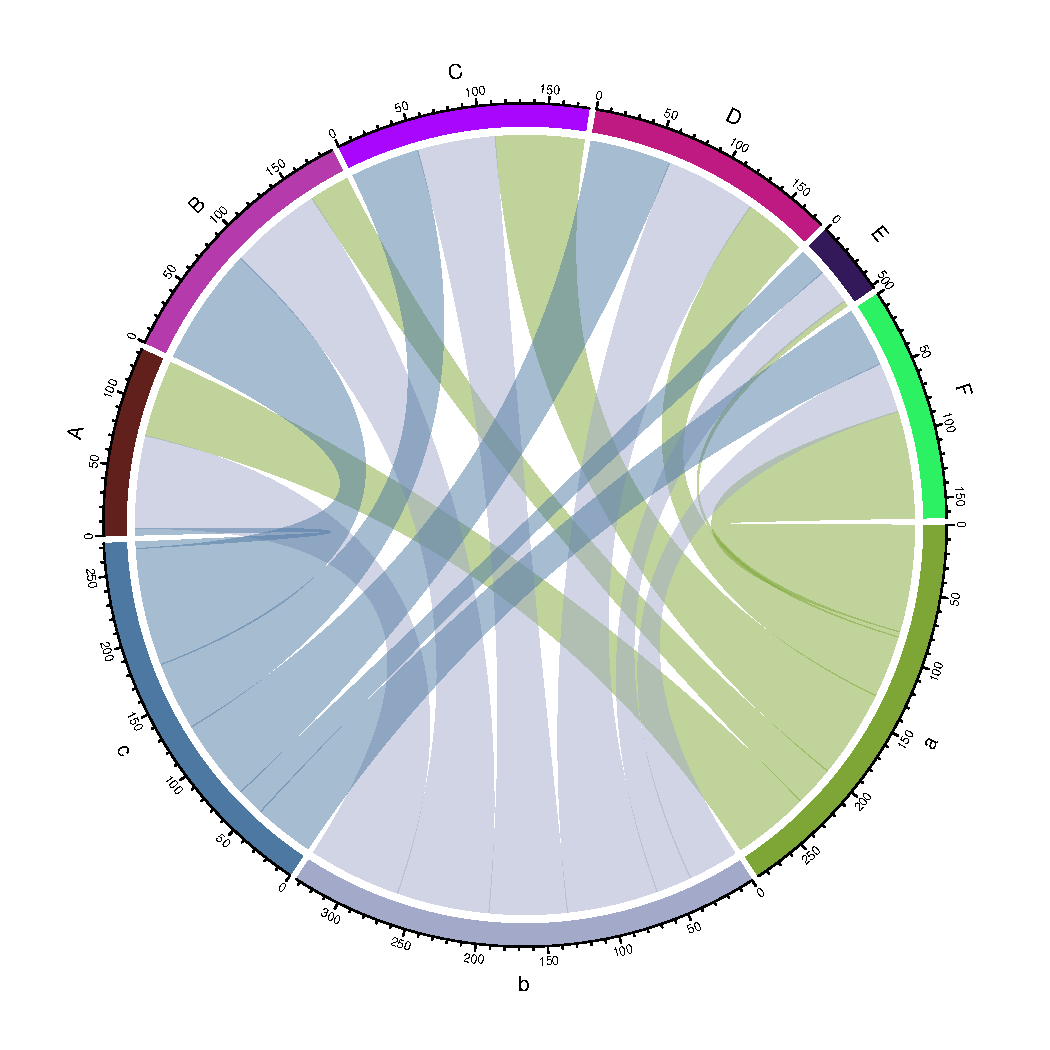
\includegraphics[width=\maxwidth]{figure/unnamed-chunk-1-1} 

\end{knitrout}
\end{tiny}
\caption{This is a \texttt{chordDiagram} plot that comes with the R package \texttt{circlize}. How fucking cool is this?! Have fun trying to make this with SPSS.}
\label{fig:chorddiagram}
\end{marginfigure}

\item Using RStudio, You can easily and seamlessly combine R code, analyses, plots, and written text into elegant documents all in one place using Sweave (R and Latex) or RMarkdown. In fact, I wrote this entire book (the text, formatting, plots, code...yes, everything) in RStudio using Sweave. With RStudio and Sweave, instead of trying to manage two or three programs, say Excel, Word and (sigh) SPSS, where you find yourself spending half your time copying, pasting and formatting data, images and test, you can do everything in one place so nothing gets misread, mistyped, or forgotten.

\item Analyses conducted in R are transparent, easily shareable, and reproducible. If you ask an SPSS user how they conducted a specific analyses, they will either A) Not remember,  B) Try (nervously) to construct an analysis procedure on the spot that makes sense - which may or may not correspond to what they actually did months or years ago, or C) Ask you what you are doing in their kitchen\footnote{Get used to the bad jokes people. Lots more where that came from.}. I used to primarily use SPSS, so I speak from experience on this. If you ask an R user (who uses good programming techniques!) how they conducted an analysis, they should always be able to show you the exact code they used. Of course, this doesn't mean that they used the appropriate analysis or interpreted it correctly, but with all the original code, any problems should be completely transparent!

\item And most importantly of all, R is the programming language of choice for pirates.

\end{enumerate}

\subsection{Code Chunks}

In this book, R code is (almost) always presented in a separate gray box like this one:


\begin{knitrout}
\definecolor{shadecolor}{rgb}{0.969, 0.969, 0.969}\color{fgcolor}\begin{kframe}
\begin{alltt}
\hlstd{a} \hlkwb{<-} \hlnum{1} \hlopt{+} \hlnum{2} \hlopt{+} \hlnum{3} \hlopt{+} \hlnum{4} \hlopt{+} \hlnum{5}
\hlstd{a}
\end{alltt}
\begin{verbatim}
## [1] 15
\end{verbatim}
\end{kframe}
\end{knitrout}

This is called a \textit{code chunk}. You should always be able to directly copy and paste code chunks directly into R. If you copy a chunk and it does not work for you, it is most likely because the code refers to a package, function, or object that I defined in a previous chunk. If so, read back and look for a previous chunk that contains the missing definition. As you'll soon learn, lines that begin with \texttt{\#} are either comments or output from prior code that R will ignore.

As you'll notice, I'll include code chunks before all plots in the book. In early chapters, the code might not make sense just yet. However, I elected to always include plotting code so you have the option of re-creating (and tweaking) any plot in the book.

\subsection{Additional Tips}

Because this is a beginner's book, I try to avoid bombarding you with too many details and tips when I first introduce a function. For this reason, at the end of every chapter, I present several tips and tricks that I think most R users should know once they get comfortable with the basics. I highly encourage you to read these additional tips as I expect you'll find at least some of them very useful if not invaluable.


\mainmatter


%----------------------------------------------------------------------------------------
%	CHAPTER 1
%----------------------------------------------------------------------------------------
\chapter{1: Getting Started (and why R is like a relationship)}
\label{ch:1}


\section{R is like a relationship...}

Yes, R is very much like a relationship. Like relationships, there are two major truths to R programming:


\begin{marginfigure}
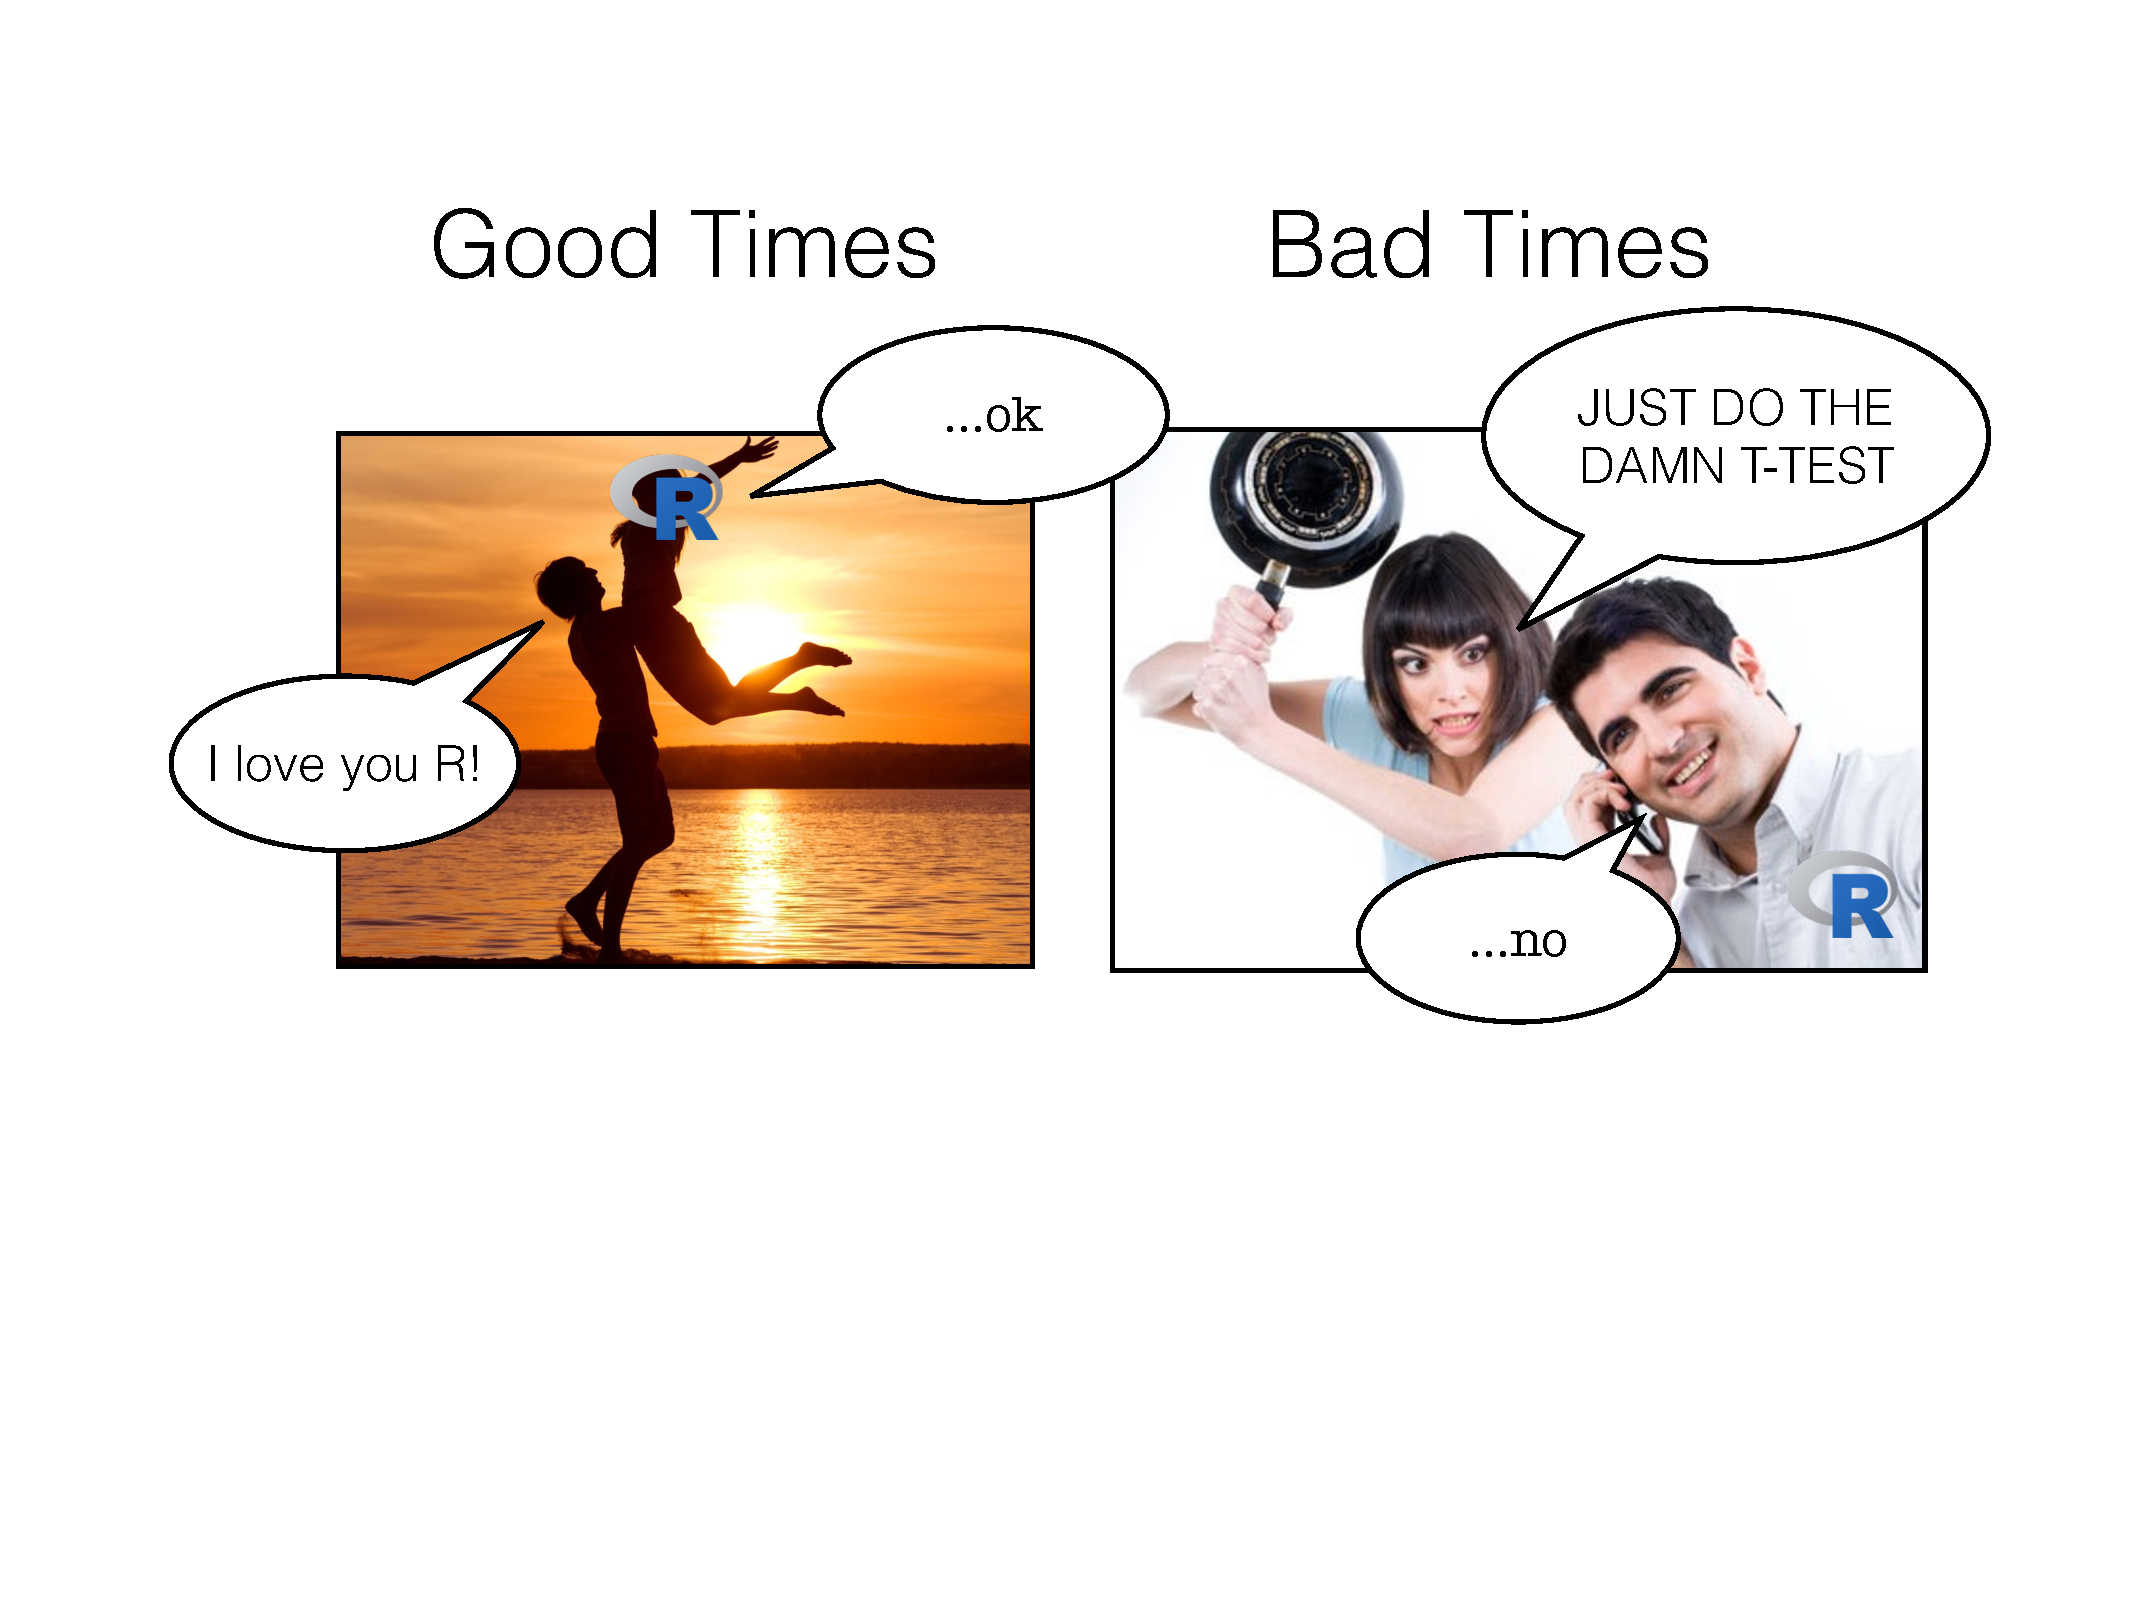
\includegraphics[width=5cm,keepaspectration]{rrelationship.pdf}
\caption{Yep, R will become both your best friend and your worst nightmare. The bad times will make the good times oh so much sweeter.}
\end{marginfigure}

\begin{large}
\begin{enumerate}

  \item There is nothing more \textit{frustrating} than when your code does \textit{not} work

  \item There is nothing more \textit{satisfying} than when your code \textit{does} work!

\end{enumerate}
\end{large}


So by now you've installed R and you're ready to get started. But first, let me give you a brief word of warning: Especially if this is your first experience programming, you are going to experience a \textit{lot} of headaches when you get started. You will run into error after error and pound your fists against the table screaming: "WHY ISN'T MY CODE WORKING?!?!? There must be something wrong with this stupid software!!!" You will spend hours trying to find a bug in your code, only to find that - frustratingly enough, you had had an extra space or missed a comma somewhere. You'll then wonder why you ever decided to learn R when (::sigh::) SPSS was so "nice and easy."

\begin{marginfigure}
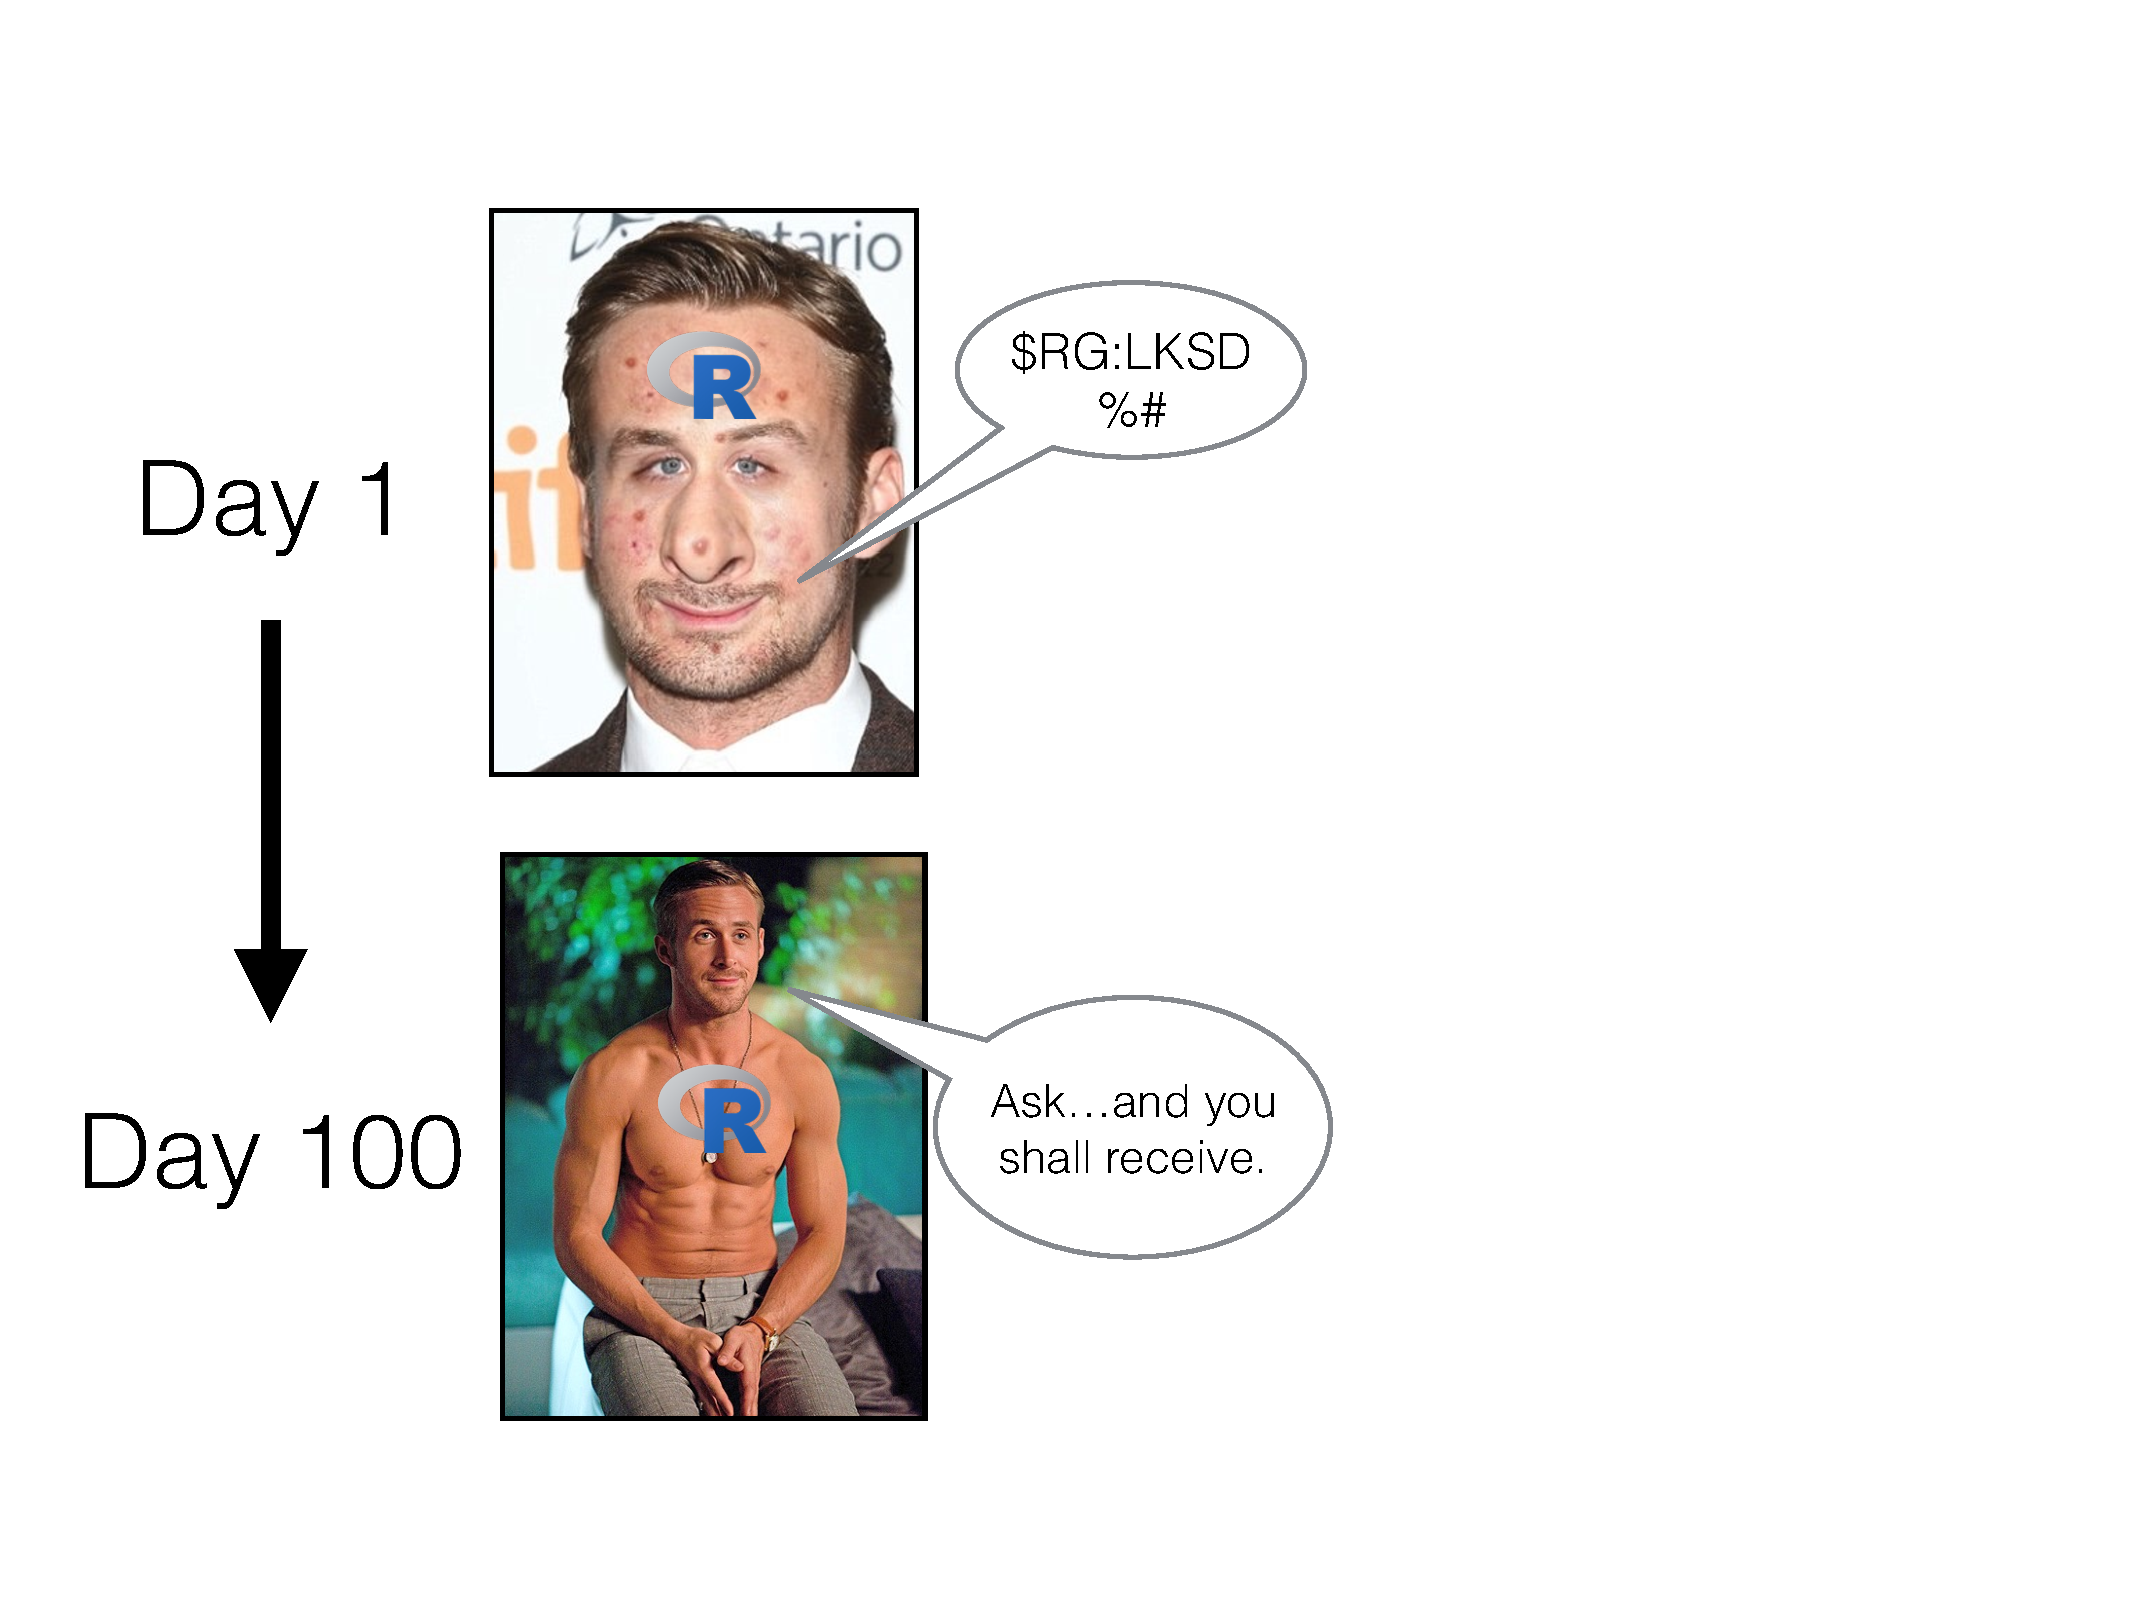
\includegraphics[width=5cm,keepaspectration]{gosling.pdf}
\caption{When you first meet R, it will look so fugly that you'll wonder if this is all some kind of sick joke. But trust me, once you learn how to talk to it, and clean it up a bit, all your friends will be crazy jealous.}
\end{marginfigure}



\marginnote{Fun fact: SPSS stands for "Shitty Piece of Shitty Shit". True story.}

This is perfectly normal! Don't get discouraged and DON'T GO BACK TO SPSS! Trust me, as you gain more programming experience, you'll experience fewer and fewer bugs (though they'll never go away completely). Once you get over the initial barriers, you'll find yourself conducting analyses much, much faster than you ever did before.

\break
\section{Installing R and RStudio}
%------------------------------------------------

First things first, let's download both Base R and Rstudio. Of course, they are totally free and open source.

\begin{table}[h!]

  \begin{tabular}{  c  c }

    \begin{minipage}{.3\textwidth}
      
\includegraphics[width=\linewidth, height=20mm]{/Users/Nathaniel/Dropbox/Git/YaRrr_Book/media/rlogo.png}
    \end{minipage} &
    \textbf{\LARGE{Download Base R}}


  \end{tabular}

\end{table}




\begin{itemize}

\item Windows: \textcolor{blue}{\href{<http://cran.r-project.org/bin/windows/base/>}{http://cran.r-project.org/bin/windows/base/}}
\item Mac: \textcolor{blue}{\href{<http://cran.r-project.org/bin/macosx/>}{http://cran.r-project.org/bin/macosx/}}

\end{itemize}

Once you've installed base R on your computer, try opening it. When you do you should see a screen like the one in Figure~\ref{fig:rscreenshot} (this is the Mac version). As you can see, base R is very much bare-bones software. It's kind of the equivalent of a simple text editor that comes with your computer.

\begin{marginfigure}
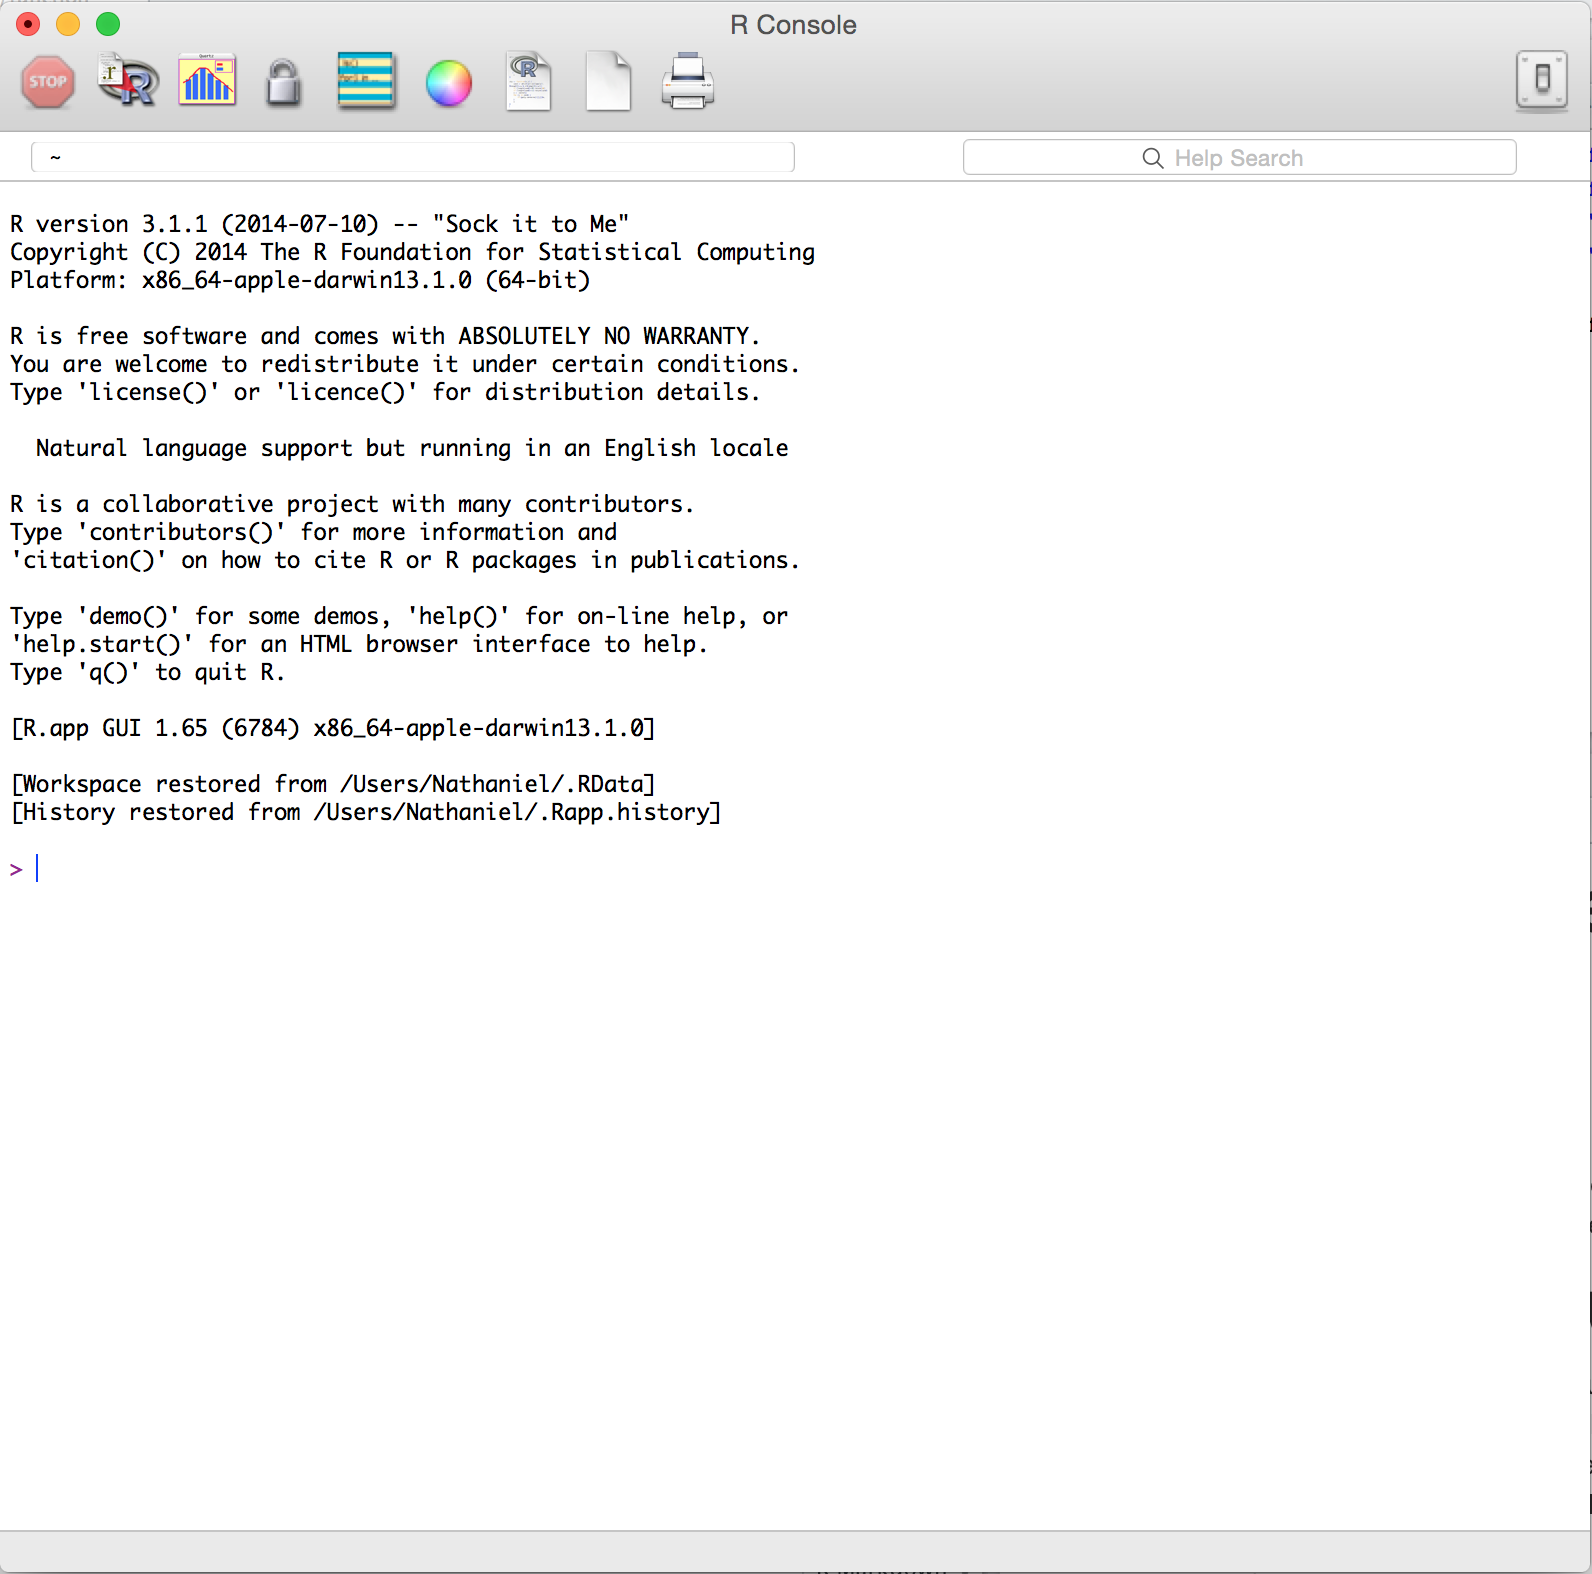
\includegraphics[width=\linewidth]{/Users/Nathaniel/Dropbox/Git/YaRrr_Book/media/RScreenshot.png}
\caption{Here is how the standard R application looks. Not too exciting - just how we like it!}
\label{fig:rscreenshot}
\end{marginfigure}



\bigskip


\begin{table}[h!]

  \begin{tabular}{  c  c }

    \begin{minipage}{.3\textwidth}
      
\includegraphics[width=\linewidth, height=20mm]{/Users/Nathaniel/Dropbox/Git/YaRrr_Book/media/rstudiologo.png}
    \end{minipage} &
    \textbf{\LARGE{Download RStudio}}


  \end{tabular}

\end{table}

\begin{itemize}

\item Windows and Mac: \textcolor{blue}{\href{<http://www.rstudio.com/products/rstudio/download/>}{http://www.rstudio.com/products/rstudio/download/}}

\end{itemize}

While you can do pretty much everything you want within base R, you'll find that most people these days do their R programming in an application called RStudio. RStudio is a graphical user interface (GUI)-like interface for R that makes programming in R a bit easier. In fact, once you've installed RStudio, you'll likely never need to open the base R application again. To download and install RStudio (around 40mb), go to one of the links above and follow the instructions.


Let's go ahead and boot up RStudio and see how she looks!

\subsection{The four RStudio windows}

When you open RStudio, you'll see the following four windows (also called panes) shown in in Figure~\ref{fig:rstudioscreen}. However, your windows might be in a different order that those in Figure~\ref{fig:rstudioscreen}. If you'd like, you can change the order of the windows under RStudio preferences. You can also change their shape by either clicking the minimize or maximize buttons on the top right of each panel, or by clicking and dragging the middle of the borders of the windows.

\begin{figure*}[h]
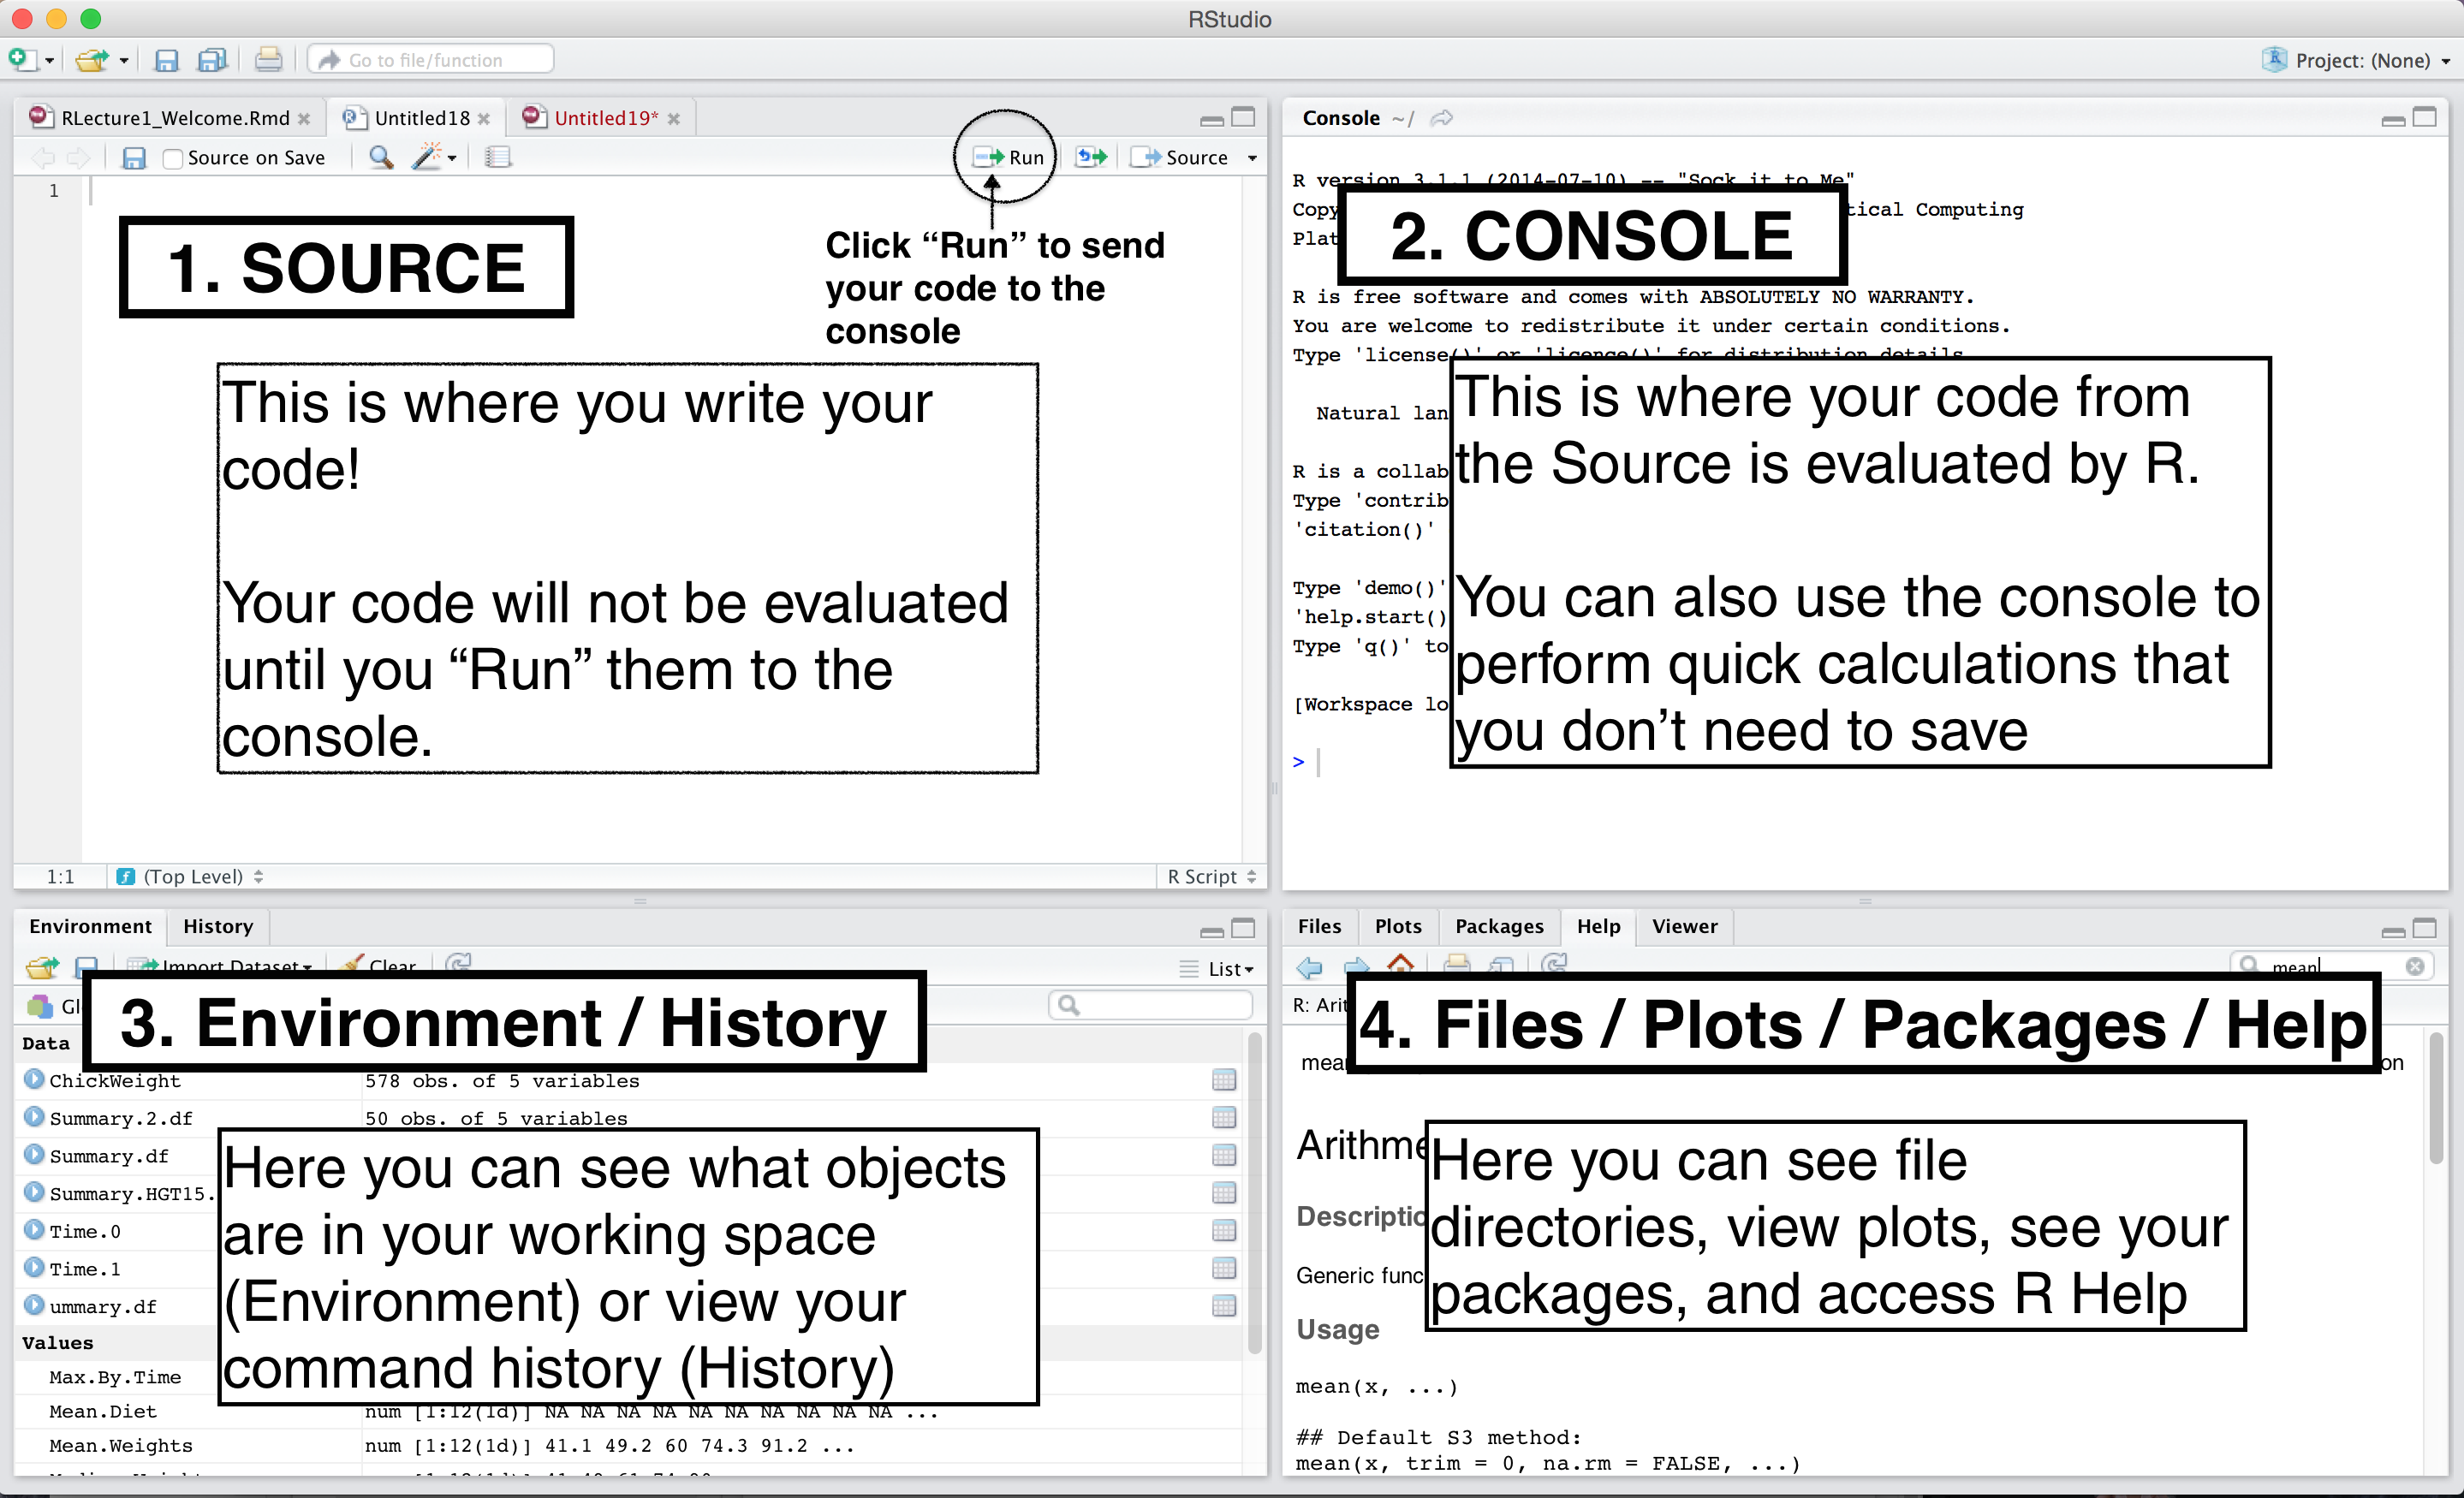
\includegraphics[width=\linewidth]{/Users/Nathaniel/Dropbox/Git/YaRrr_Book/media/RStudio_Screenshot_Labels.png}
\caption{The four panes of RStudio.}
\label{fig:rstudioscreen}
\end{figure*}


Now, let's see what each window does in detail.

\subsection{Source - Your notepad for code}

The source pane is where you create and edit ``R Scripts" - your collections of code. Don't worry, R scripts are just text files with the ".R" extension. When you open RStudio, it will automatically start a new Untitled script. Before you start typing in an untitled R script, you should always save the file under a new file name (like, "2015PirateSurvey.R"). That way, if something on your computer crashes while you're working, R will have your code waiting for you when you re-open RStudio.

You'll notice that when you're typing code in a script in the Source panel, R won't actually evaluate the code as you type. To have R actually evaluate your code, you need to first 'send' the code to the Console (we'll talk about this in the next section).

There are many ways to send your code from the Source to the console. The slowest way is to copy and paste. A faster way is to highlight the code you wish to evaluate and clicking on the "Run" button on the top right of the Source. Alternatively, you can use the hot-key "Command + Return" on Mac, or "Control + Enter" on PC to send all highlighted code to the console.

\subsection{Console: The calculator}

The console is where R actually evaluates code. At the beginning of the console you'll see the character \texttt{>}. This is a prompt that tells you that R is ready for new code. You can type code directly into the console after the \texttt{>} prompt and get an immediate response. For example, if you type 1+1 into the console and press enter, you'll see that R immediately gives an output of 2.


\begin{knitrout}
\definecolor{shadecolor}{rgb}{0.969, 0.969, 0.969}\color{fgcolor}\begin{kframe}
\begin{alltt}
\hlnum{1}\hlopt{+}\hlnum{1}
\end{alltt}
\begin{verbatim}
## [1] 2
\end{verbatim}
\end{kframe}
\end{knitrout}


Try calculating 1+1 by typing the code directly into the console - then press Enter. You should see the result [1] 2. Don't worry about the [1] for now, we'll get to that later. For now, we're happy if we just see the 2. Then, type the same code into the Source, and then send the code to the Console by highlighting the code and clicking the ``Run" button on the top right hand corner of the Source window. Alternatively, you can use the hot-key "Command + Return" on Mac or "Control + Enter" on Windows.

\marginnote{Tip: Try to write most of your code in a document in the Source. Only type directly into the Console to de-bug or do quick analyses.}

So as you can see, you can execute code either by running it from the Source or by typing it directly into the Console. However, 99\% most of the time, you should be using the Source rather than the Console. The reason for this is straightforward: If you type code into the console, it won't be saved (though you can look back on your command History). And if you make a mistake in typing code into the console, you'd have to re-type everything all over again. Instead, it's better to write all your code in the Source. When you are ready to execute some code, you can then send "Run" it to the console.

\subsection{Environment / History}

The Environment tab of this panel shows you the names of all the data objects (like vectors, matrices, and dataframes) that you've defined in your current R session. You can also see information like the number of observations and rows in data objects. The tab also has a few clickable actions like ``Import Dataset" which will open a graphical user interface (GUI) for important data into R. However, I almost never look at this menu.

The History tab of this panel simply shows you a history of all the code you've previously evaluated in the Console. To be honest, I never look at this. In fact, I didn't realize it was even there until I started writing this tutorial.

As you get more comfortable with R, you might find the Environment / History panel useful. But for now you can just ignore it. If you want to declutter your screen, you can even just minimize the window by clicking the minimize button on the top right of the panel.

\subsection{Files / Plots / Packages / Help}

The Files / Plots / Packages / Help panel shows you lots of helpful information. Let's go through each tab in detail:

\begin{enumerate}

\item Files - The files panel gives you access to the file directory on your harddrive. One nice feature of the "Files" panel is that you can use it to set your working directory - once you navigate to a folder you want to read and save files to, click "More" and then "Set As Working Directory." We'll talk about working directories in more detail soon.

\item Plots - The Plots panel (no big surprise), shows all your plots. There are buttons for opening the plot in a separate window and exporting the plot as a pdf or jpeg (though you can also do this with code using the \texttt{pdf()} or \texttt{jpeg()} functions.)\marginnote{Most - if not all - of the time when you perform actions using your mouse by pointing and clicking in RStudio, RStudio will perform the function by sending the appropriate R Code to the console. You can then copy and paste this code into your documents to automate the process later.}

Let's see how plots are displayed in the Plots panel. Run the following code to display a histogram of 100 values randomly drawn from a standard normal distribution. When you do, you should see a plot similar to this one show up in the Plots panel. Don't worry if your plot looks slightly different from this one: as you'll learn later, the rnorm() function generates different data each time you evaluate it!


\begin{knitrout}
\definecolor{shadecolor}{rgb}{0.969, 0.969, 0.969}\color{fgcolor}\begin{kframe}
\begin{alltt}
\hlkwd{hist}\hlstd{(}\hlkwc{x} \hlstd{=} \hlkwd{rnorm}\hlstd{(}\hlkwc{n} \hlstd{=} \hlnum{100}\hlstd{,} \hlkwc{mean} \hlstd{=} \hlnum{1000}\hlstd{,} \hlkwc{sd} \hlstd{=} \hlnum{100}\hlstd{),}
     \hlkwc{main} \hlstd{=} \hlstr{"Plunder in 2015"}\hlstd{,}
     \hlkwc{xlab} \hlstd{=} \hlstr{"Amount"}
     \hlstd{)}
\end{alltt}
\end{kframe}
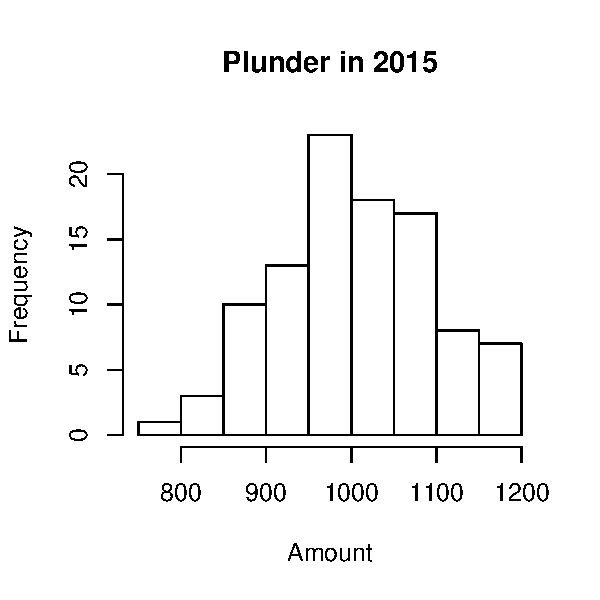
\includegraphics[width=\maxwidth]{figure/unnamed-chunk-4-1} 

\end{knitrout}



\item Packages - Shows a list of all the R packages installed on your harddrive and indicates whether or not they are currently loaded. Packages that are loaded in the current session are checked while those that are installed but not yet loaded are unchecked. We'll discuss packages in more detail in the next section.

\item Help - Help menu for R functions. You can either type the name of a function in the search window, or use the code \texttt{?function.name} to search for a function with the name \texttt{function.name}

To get help and see documentation for a function, type \texttt{?fun}, where \texttt{fun} is the name of the function. For example, to get additional information on the histogram function, run the following code:

\marginnote{Tip: If you ever need to learn more about an R function: type \texttt{?functionname}, where \texttt{functionname} is the name of the function.}

\begin{footnotesize}
\begin{knitrout}
\definecolor{shadecolor}{rgb}{0.969, 0.969, 0.969}\color{fgcolor}\begin{kframe}
\begin{alltt}
\hlopt{?}\hlstd{hist}
\end{alltt}
\end{kframe}
\end{knitrout}
\end{footnotesize}

\end{enumerate}


\section{Installing and loading packages}

When you download and install R for the first time, you are installing the Base R software. Base R will will contain most if not all the functions you need. However, one of the great things about R is that people are constantly writing and sharing new functions that you can use. When people share a new function, they usually do so in the form of an \textit{R package} which contains anything from functions, to help menus, to vignettes (examples), to data.

Most R packages are hosted at the Comprehensive R Archive Network (CRAN) \textcolor{blue}{\href{<https://cran.r-project.org/>}{https://cran.r-project.org/}}. To install a new R package from CRAN, you can simply run the code \texttt{install.packages("package")}, where "package" is the name of the package. After you've installed the package, you need to \textit{load} it into R by running the code \texttt{library("package")}. This will load the package into your current R session and allow you to use its contents.\marginnote{Once you've installed a package on your computer, you never need to install it again. However, you do need to load the package every time you start a new R session.}

To see how this works in action, let's install and load the \texttt{wordcloud} package. This package contains the \texttt{wordcloud} function which allows you to easily create those really cool wordcloud plots you've seen on the Internets.

We'll start by installing the package. When you run the following code, R will download the package from CRAN. If everything works, you should see some information about where the package is being downloaded from, in addition to a progress bar.

\begin{knitrout}
\definecolor{shadecolor}{rgb}{0.969, 0.969, 0.969}\color{fgcolor}\begin{kframe}
\begin{alltt}
\hlkwd{install.packages}\hlstd{(}\hlstr{"wordcloud"}\hlstd{)}
\end{alltt}
\end{kframe}
\end{knitrout}

Now that the package is installed on your computer, you can use it anytime you want by loading the package:

\begin{knitrout}
\definecolor{shadecolor}{rgb}{0.969, 0.969, 0.969}\color{fgcolor}\begin{kframe}
\begin{alltt}
\hlkwd{library}\hlstd{(}\hlstr{"wordcloud"}\hlstd{)}
\end{alltt}


{\ttfamily\noindent\itshape\color{messagecolor}{\#\# Loading required package: RColorBrewer}}\end{kframe}
\end{knitrout}

Now, let's create a wordcloud of pirate words! Don't worry about the specifics of the code below, you'll learn more about how all this works later. For now, just run the code and marvel at your wordcloud!

\begin{knitrout}
\definecolor{shadecolor}{rgb}{0.969, 0.969, 0.969}\color{fgcolor}\begin{kframe}
\begin{alltt}
\hlkwd{wordcloud}\hlstd{(}\hlkwc{words} \hlstd{=} \hlkwd{c}\hlstd{(}\hlstr{"Blackbeard"}\hlstd{,} \hlstr{"Jolly.Roger"}\hlstd{,} \hlstr{"Grogg"}\hlstd{,} \hlstr{"Monkey.Island"}\hlstd{,} \hlstr{"Treasure"}\hlstd{,} \hlstr{"cutlass"}\hlstd{),}
              \hlkwc{freq} \hlstd{=} \hlkwd{c}\hlstd{(}\hlnum{100}\hlstd{,} \hlnum{20}\hlstd{,} \hlnum{50}\hlstd{,} \hlnum{40}\hlstd{,} \hlnum{200}\hlstd{,} \hlnum{100}\hlstd{))}
\end{alltt}
\end{kframe}
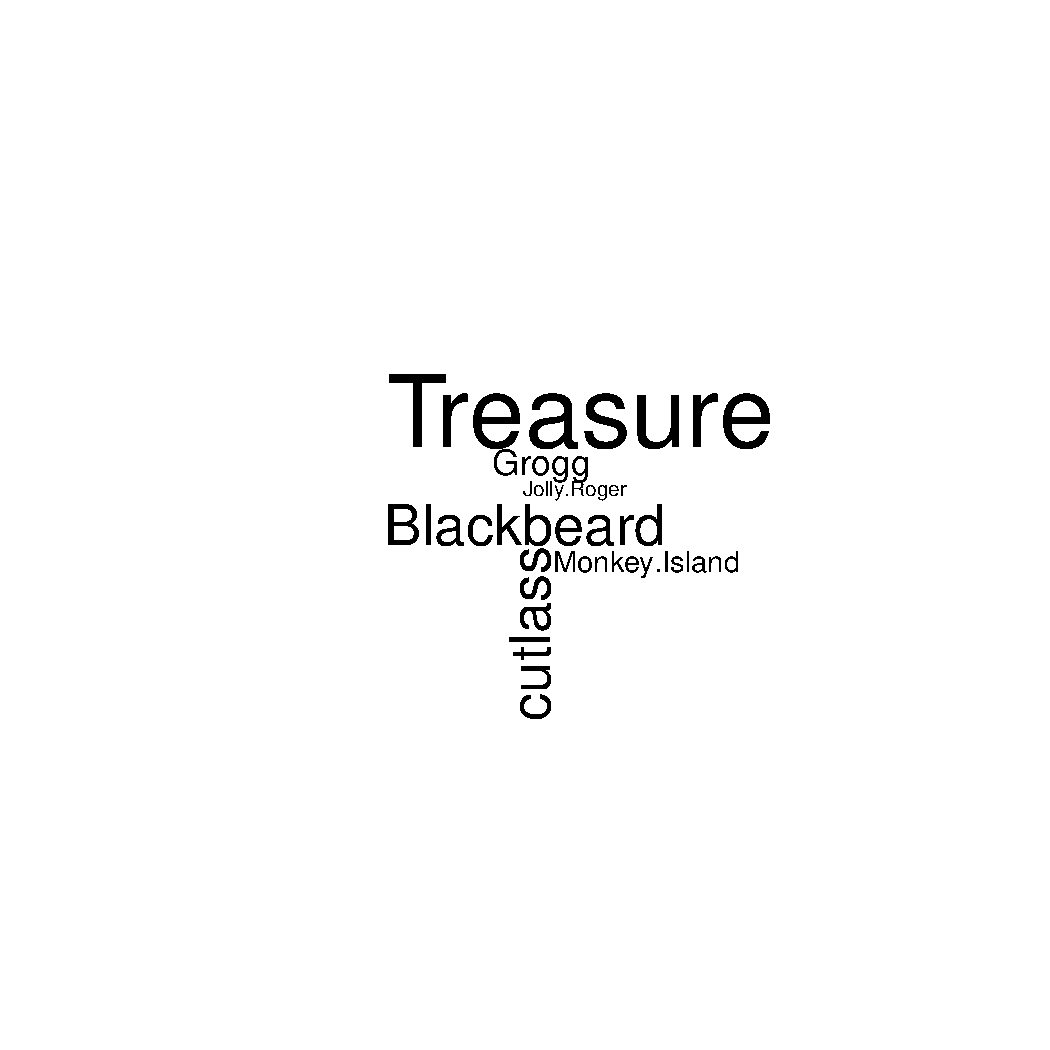
\includegraphics[width=\maxwidth]{figure/unnamed-chunk-8-1} 

\end{knitrout}


\section{The yarrr package}

For much of this book, you will need the \texttt{yarrr} package. This package contains every dataset, function, and plotting code from this book. Unlike most packages that you'll be using, the \texttt{yarrr} package is not hosted at CRAN. Instead, all the code is on github\footnote{For those of you unfamiliar with github, it's basically Facebook for programmers.} at \textcolor{blue}{\href{<www.github.com/ndphillips/yarrr>}{www.github.com/ndphillips/yarrr}}. To install the \texttt{yarrr} package on your machine, you'll first need to install the \texttt{devtools} package which will then allow you to directly install packages from github:

\begin{knitrout}
\definecolor{shadecolor}{rgb}{0.969, 0.969, 0.969}\color{fgcolor}\begin{kframe}
\begin{alltt}
\hlkwd{install.packages}\hlstd{(}\hlstr{"devtools"}\hlstd{)} \hlcom{# Install the devtools package}
\end{alltt}
\end{kframe}
\end{knitrout}

Now that you've installed and loaded the \textt{devtools} package, you can install and load the \texttt{yarrr} package from github with the following code:


\begin{knitrout}
\definecolor{shadecolor}{rgb}{0.969, 0.969, 0.969}\color{fgcolor}\begin{kframe}
\begin{alltt}
\hlstd{devtools}\hlopt{::}\hlkwd{install_github}\hlstd{(}\hlstr{"ndphillips/yarrr"}\hlstd{)} \hlcom{# Install the yarrr package}
\end{alltt}
\end{kframe}
\end{knitrout}



If everything went correctly, you should have access to all the datasets mentioned in this book in addition to many functions like \texttt{apa()} and \texttt{pirateplot()}.

\marginnote{Don't worry if you are unable to install the yarrr package. I'll also provide direct html links that you can use the download the datasets when necessary.}

To see the dataset, you can execute the the \texttt{View()} function:

\begin{knitrout}
\definecolor{shadecolor}{rgb}{0.969, 0.969, 0.969}\color{fgcolor}\begin{kframe}
\begin{alltt}
\hlkwd{View}\hlstd{(pirates)}
\end{alltt}
\end{kframe}
\end{knitrout}

When you run this command, you should see the first several rows and columns of the dataset (like this:)

\begin{figure*}
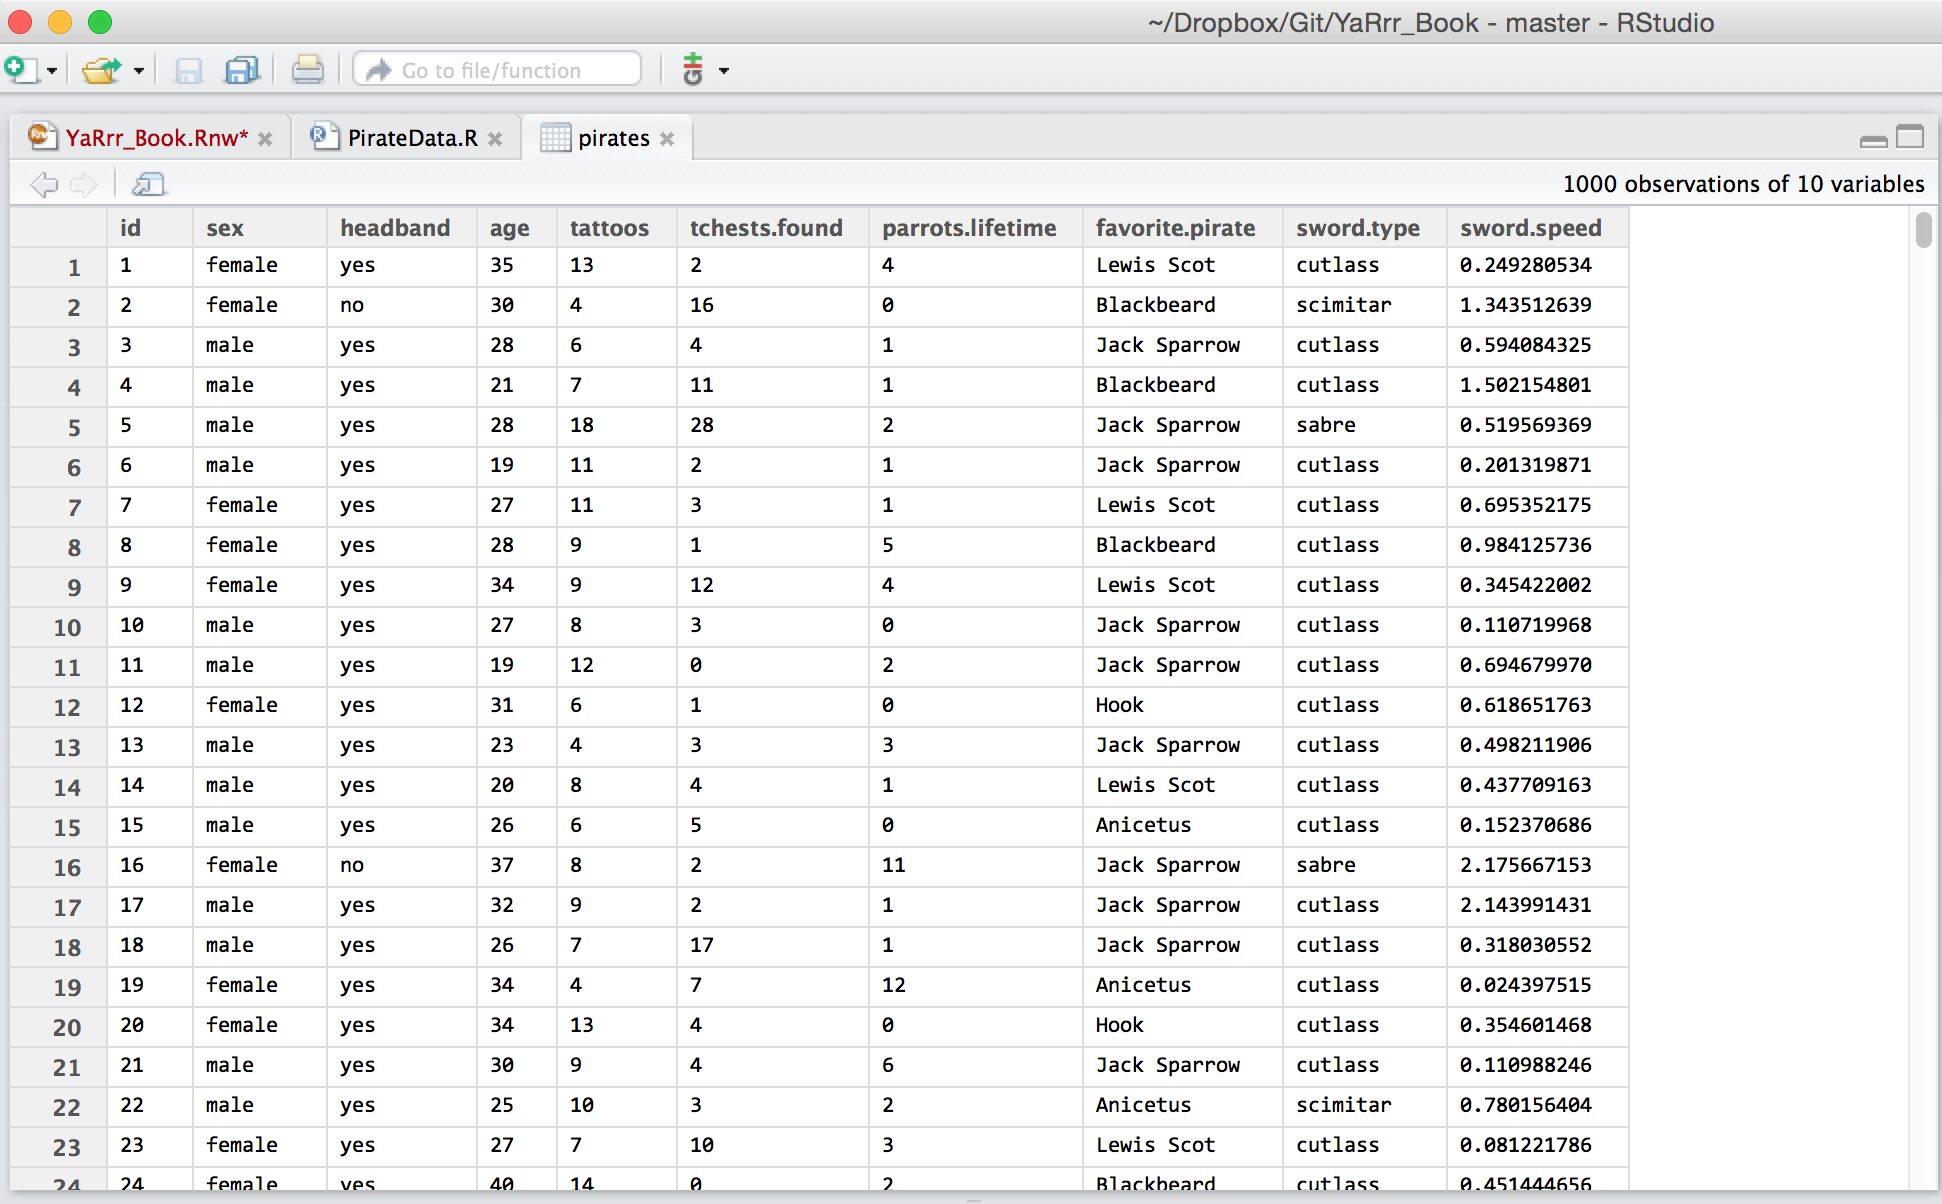
\includegraphics[width=\linewidth]{/Users/Nathaniel/Dropbox/Git/YaRrr_Book/media/pirates_data_screenshot.png}
\caption{The pirates dataset included in the yarrr package.}
\label{fig:piratesdata}
\end{figure*}


If you were unable to download the yarrr package and access the pirates dataset (this can happen on some computers depending on many possible issues), you can also use the following code to download the dataset directly from the web:

\begin{footnotesize}
\begin{knitrout}
\definecolor{shadecolor}{rgb}{0.969, 0.969, 0.969}\color{fgcolor}\begin{kframe}
\begin{alltt}
\hlstd{pirates} \hlkwb{<-} \hlkwd{read.table}\hlstd{(}\hlkwc{file} \hlstd{=} \hlstr{"http://nathanieldphillips.com/wp-content/uploads/2015/11/pirates1.txt"}\hlstd{,}
                      \hlkwc{header} \hlstd{= T,}
                      \hlkwc{sep} \hlstd{=} \hlstr{"\textbackslash{}t"}\hlstd{,} \hlcom{# tab-delimited}
                      \hlkwc{stringsAsFactors} \hlstd{= F}
                      \hlstd{)}
\end{alltt}
\end{kframe}
\end{knitrout}
\end{footnotesize}




\section{The R Reference Card}

Over the course of this book, you will be learning \textit{lots} of new functions. Wouldn't it be nice if someone created a Cheatsheet / Notecard of many common R functions? Yes it would, and thankfully Tom Short has done this in his creation of the R Reference Card. I highly encourage you to print this out and start highlighting functions as you learn them!
.

You can access the pdf of this card in two ways. You can get it on the web at \textcolor{blue}{\href{<http://nathanieldphillips.com/wp-content/uploads/2015/09/R-Reference-Card.pdf>}{http://nathanieldphillips.com/wp-content/uploads/2015/09/R-Reference-Card.pdf}}. Alternatively, you can get it from the yarrr package. To find where the file is located on your computer, run the following code (the output after the code is the file location on my computer):

\begin{knitrout}
\definecolor{shadecolor}{rgb}{0.969, 0.969, 0.969}\color{fgcolor}\begin{kframe}
\begin{alltt}
\hlkwd{system.file}\hlstd{(}\hlstr{"RReferenceCard.pdf"}\hlstd{,} \hlkwc{package}\hlstd{=}\hlstr{"yarrr"}\hlstd{)}
\end{alltt}
\begin{verbatim}
## [1] "/Library/Frameworks/R.framework/Versions/3.2/Resources/library/yarrr/RReferenceCard.pdf"
\end{verbatim}
\end{kframe}
\end{knitrout}


\subsection{Finished!}

That's it for this lecture! All you did was install the most powerful statistical package on the planet used by top universities and companies like Google. No big deal.

%----------------------------------------------------------------------------------------
%	CHAPTER 2
%----------------------------------------------------------------------------------------

\chapter{2: Coding Basics}
\label{ch:2}


\subsection{Chapter Goals}

\begin{enumerate}
  \item Accept that learning R will take time (and promise you'll never go back to SPSS!)
  \item Know how to use comments and spaces in R code.
  \item Be able to define and manipulate scalars and vectors
  \item Generate vectors using c(), :, rep(), and seq()
\end{enumerate}



\subsection{The basics of R programming}

Ok, let's write some code! Again, we will write all our code in a script file in the Source pane of RStudio. When we want to execute it, we'll send it to the Console.

\subsection{R as a calculator}


\begin{marginfigure}
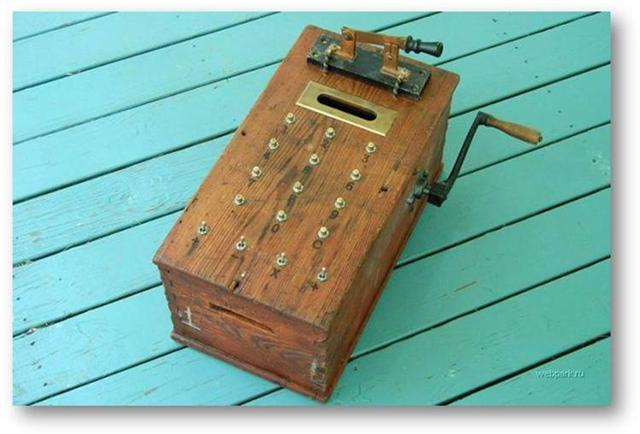
\includegraphics[width=\linewidth]{woodcalc.jpg}
\caption{Yep. R is really just a fancy calculator. This R programming device was found on a shipwreck on the Bodensee in Germany. I stole it from a museum and made a pretty sweet plot with it. But I don't want to show it to you.}
\end{marginfigure}

At its heart, R is just a fancy calculator. Let's do some basic algebra, type the following command into the source, then highlight the text and click "Run" to execute it in the console:

\marginnote{Tip: To execute code from the source to the console, highlight it and use the hot-keys "Command-Return" on Mac or "Control-Enter" on PC.}


\begin{knitrout}
\definecolor{shadecolor}{rgb}{0.969, 0.969, 0.969}\color{fgcolor}\begin{kframe}
\begin{alltt}
\hlnum{1}\hlopt{+}\hlnum{1}
\end{alltt}
\begin{verbatim}
## [1] 2
\end{verbatim}
\end{kframe}
\end{knitrout}



As you can see, R returns the (thankfully correct) value of 2. You'll notice that the console also returns the text [1]. This is just telling you you the index of the value next to it. Don't worry about this for now, it will make more sense later.

\subsection{Commenting code with the # (pound) sign}

Additionally, you'll notice that I included a comment in the code using the \# sign. R will ignore everything on a line after the \# sign. So why do we use comments? Mainly to explain to others, including your future self, what you are trying to do with your code.\marginnote{Do your future self a favor and use comments to explain what you're doing with your code. Also, maybe go for a run once in a while.}

\begin{knitrout}
\definecolor{shadecolor}{rgb}{0.969, 0.969, 0.969}\color{fgcolor}\begin{kframe}
\begin{alltt}
\hlcom{# This is a comment, R will ignore everything on this line}

\hlnum{1} \hlopt{+} \hlnum{1} \hlcom{# You can put comments on the same line after code}
\end{alltt}
\begin{verbatim}
## [1] 2
\end{verbatim}
\begin{alltt}
\hlcom{# Note to self: Put on an Evil Dead marathon with Bloody Mary's}
\end{alltt}
\end{kframe}
\end{knitrout}

\subsection{Code formatting guidelines}

\begin{marginfigure}

\includegraphics[width=\linewidth]{futureself.jpg}
\caption{As Stan discovered in season six of South Park, your future self is a lazy, possibly intoxicated moron. So do your future self a favor and make your code look nice.}
\end{marginfigure}

While it's important that R understands your code, it's equally as important that other humans (including your future self) understand your code. For this reason, it's important to make appropriate use of spaces, line breaks, and comments. For example, I include spaces between arithmetic operators (like =, + and -) and after commas (which we'll get to later). Personally, this makes code much easier for me to follow. For a list of recommendations on how to make your code easier to follow, check out Google's own company R Style guide at \textcolor{blue}{\href{<https://google-styleguide.googlecode.com/svn/trunk/Rguide.xml>}{https://google-styleguide.googlecode.com/svn/trunk/Rguide.xml}}

\section{Assigning objects with the <- assignment}

\marginnote{Good object names strike a balance between being easy to type (i.e.; short names) and interpret. If you have several datasets, it's probably not a good idea to name them \texttt{a}, \texttt{b}, \texttt{c} because you'll forget which is which. However, using long names like \texttt{March2015Group1OnlyFemales} and \texttt{March2015Group1OnlyMales} will give you carpel tunnel syndrome.}

So far so good, you can use R as a simple calculator. Now, let's do our first \textit{object assignment}.

Object assignment is our way of storing information, such as a number or a statistical test, into something we can easily refer to later. This is a pretty big deal. Object assignment allows us to store data objects under relevant names which we can then use to slice and dice specific data objects anytime we'd like to.

To do an assignment, we use the almighty <- operator.

\newfun{new.object <- something}\index{assignment}

\marginnote{
\center{
\Huge{a <- b}
}

}

To assign something to a new object (or to update an existing object), use the notation \texttt{new.object <- something}, where \texttt{new.object} is the new (or updated) object, and \texttt{something} is whatever you want to store in \texttt{new.object}.

Let's start by creating a very simple object called \texttt{a} and assigning the value of 100 to it:

\begin{knitrout}
\definecolor{shadecolor}{rgb}{0.969, 0.969, 0.969}\color{fgcolor}\begin{kframe}
\begin{alltt}
\hlstd{a} \hlkwb{<-} \hlnum{100} \hlcom{# Assign the value of 100 to a new object called a}
\end{alltt}
\end{kframe}
\end{knitrout}

Now, anytime we want to refer to the content of the object \texttt{a}, we can just type it. You may have noticed that when you run the code above, R won't actually show you the value of \texttt{a}. If you want to see the value, you need to call the object by just executing its name:

\begin{knitrout}
\definecolor{shadecolor}{rgb}{0.969, 0.969, 0.969}\color{fgcolor}\begin{kframe}
\begin{alltt}
\hlstd{a}
\end{alltt}
\begin{verbatim}
## [1] 100
\end{verbatim}
\end{kframe}
\end{knitrout}

Now, R will print the value of \texttt{a} (in this case 100) to the console.

\marginnote{You can use \texttt{=} instead of \texttt{<-} for object assignment but I recommend you stick with \textt{<-} because the direction of the assignment is clear.}

\subsection{How to name objects}

You can create object names using any combination of letters and a few special characters (like \texttt{.}). However, you can't start the name of an object with a number, or use spaces in an object name. Let's create some new objects with meaningful names:

\begin{knitrout}
\definecolor{shadecolor}{rgb}{0.969, 0.969, 0.969}\color{fgcolor}\begin{kframe}
\begin{alltt}
\hlstd{group.mean} \hlkwb{<-} \hlnum{10.21}
\hlstd{my.age} \hlkwb{<-} \hlnum{32}
\hlstd{FavoritePirate} \hlkwb{<-} \hlstr{"Jack Sparrow"}
\hlstd{sum.1.to.5} \hlkwb{<-} \hlnum{1} \hlopt{+} \hlnum{2} \hlopt{+} \hlnum{3} \hlopt{+} \hlnum{4} \hlopt{+} \hlnum{5}
\end{alltt}
\end{kframe}
\end{knitrout}

All the object names above are perfectly valid. Now, let's look at some examples of \textit{invalid} object names which contain either spaces, start with numbers, or have invalid characters:

\begin{knitrout}
\definecolor{shadecolor}{rgb}{0.969, 0.969, 0.969}\color{fgcolor}\begin{kframe}
\begin{alltt}
a b <- 50 \hlcom{# Can't have spaces}
5a <- 50 \hlcom{# Can't start a name with a number}
a! <- 5 0# Can't have an \hlstr{"!"} in the object name
\end{alltt}
\end{kframe}
\end{knitrout}

If you try running the code above in R, you will receive a warning message starting with \texttt{Error: unexpected symbol}. Anytime you see this warning in R, it almost always means that you have a syntax error of some kind.

\subsection{R is case-sensitive!}

Like English, R is case-sensitive. This means that R treats capital letters differently from lower-case letters. For example, the four following objects \texttt{Plunder}, \texttt{plunder} and \texttt{PLUNDER} are totally different objects in R:


\begin{marginfigure}
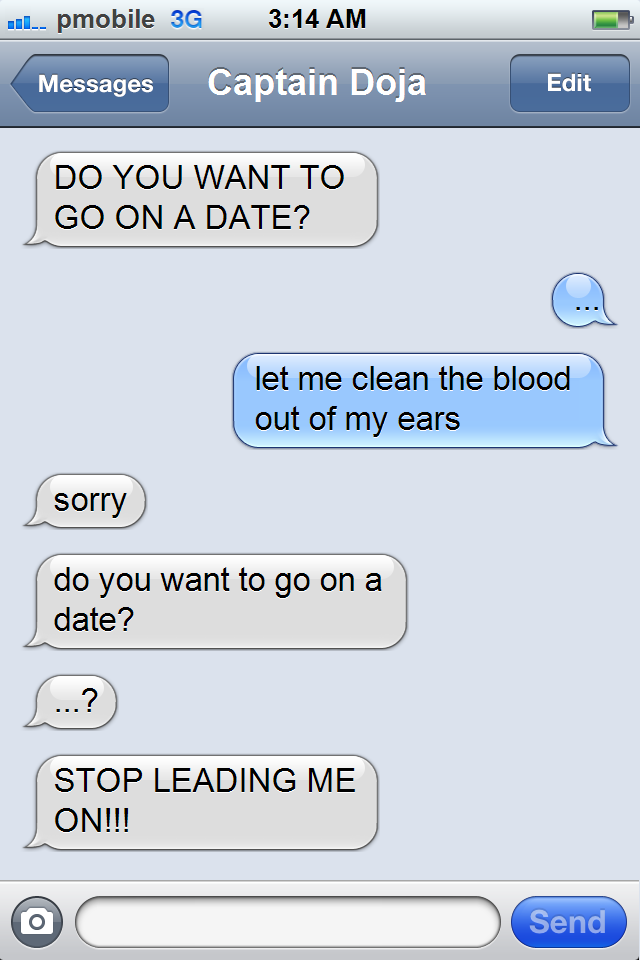
\includegraphics[width=\linewidth]{datetext.png}
\caption{Like a text message, you should probably watch your use of capitalization in R.}
\end{marginfigure}


\begin{knitrout}
\definecolor{shadecolor}{rgb}{0.969, 0.969, 0.969}\color{fgcolor}\begin{kframe}
\begin{alltt}
\hlstd{Plunder} \hlkwb{<-} \hlnum{1}
\hlstd{plunder} \hlkwb{<-} \hlnum{100}
\hlstd{PLUNDER} \hlkwb{<-} \hlnum{5}

\hlstd{Plunder}
\end{alltt}
\begin{verbatim}
## [1] 1
\end{verbatim}
\begin{alltt}
\hlstd{plunder}
\end{alltt}
\begin{verbatim}
## [1] 100
\end{verbatim}
\begin{alltt}
\hlstd{PLUNDER}
\end{alltt}
\begin{verbatim}
## [1] 5
\end{verbatim}
\end{kframe}
\end{knitrout}

Avoid using too many capital letters in object names because they require you to hold the shift key. This may sound silly, but you'd be surprised how much easier it is to type \texttt{mydata} than \texttt{MyData} 100 times.

\subsection{Changing and combining objects}

Once you've defined an object, you can change it by reassigning it, or combine it with other objects using basic arithmetic.

\begin{knitrout}
\definecolor{shadecolor}{rgb}{0.969, 0.969, 0.969}\color{fgcolor}\begin{kframe}
\begin{alltt}
\hlcom{# Set a to 100, then add 100 to it}
\hlstd{a} \hlkwb{<-} \hlnum{100}
\hlstd{a} \hlkwb{<-} \hlstd{a} \hlopt{+} \hlnum{100}
\hlstd{a}
\end{alltt}
\begin{verbatim}
## [1] 200
\end{verbatim}
\begin{alltt}
\hlcom{# Set b to a times 5}
\hlstd{b} \hlkwb{<-} \hlstd{a} \hlopt{*} \hlnum{5}
\hlstd{b}
\end{alltt}
\begin{verbatim}
## [1] 1000
\end{verbatim}
\begin{alltt}
\hlcom{# Now let's set a to 1}
\hlstd{a} \hlkwb{<-} \hlnum{1}
\hlstd{a}
\end{alltt}
\begin{verbatim}
## [1] 1
\end{verbatim}
\end{kframe}
\end{knitrout}


\marginnote{Tip: To change (reassign) an object, you have to use the <- operator - If you don't, the object won't change. In the following example, the object a does not change because we did not reassign it with <- :}

\begin{marginfigure}
\begin{knitrout}
\definecolor{shadecolor}{rgb}{0.969, 0.969, 0.969}\color{fgcolor}\begin{kframe}
\begin{alltt}
\hlstd{a} \hlkwb{<-} \hlnum{1}
\hlstd{a} \hlopt{+} \hlnum{99} \hlcom{# this will just print a + 99}
\end{alltt}
\begin{verbatim}
## [1] 100
\end{verbatim}
\begin{alltt}
\hlstd{a} \hlcom{# a is still just 1}
\end{alltt}
\begin{verbatim}
## [1] 1
\end{verbatim}
\end{kframe}
\end{knitrout}
\end{marginfigure}


\marginnote{Now, let's fix the code by reassigning a to a + 99}

\begin{marginfigure}
\begin{knitrout}
\definecolor{shadecolor}{rgb}{0.969, 0.969, 0.969}\color{fgcolor}\begin{kframe}
\begin{alltt}
\hlstd{a} \hlkwb{<-} \hlnum{1}
\hlstd{a} \hlkwb{<-} \hlstd{a} \hlopt{+} \hlnum{99}
\hlstd{a} \hlcom{# Now a is 100}
\end{alltt}
\begin{verbatim}
## [1] 100
\end{verbatim}
\end{kframe}
\end{knitrout}
\end{marginfigure}


Let's define an object called \texttt{blackpearl.usd} which has the global revenue of Pirates of the Caribbean 1 "Curse of the Black Pearl" in U.S. dollars. A quick Google search showed me that the revenue was \$634,954,103:

\begin{knitrout}
\definecolor{shadecolor}{rgb}{0.969, 0.969, 0.969}\color{fgcolor}\begin{kframe}
\begin{alltt}
\hlstd{blackpearl.usd} \hlkwb{<-} \hlnum{634954103}
\end{alltt}
\end{kframe}
\end{knitrout}

Now, my German friends might want to know how much this is in Euros. Let's create a new object called \texttt{blackpearl.eur} which converts our original value to Euros by multiplying the original amount by 0.88 (assuming 1 USD = 0.88 EUR)

\begin{knitrout}
\definecolor{shadecolor}{rgb}{0.969, 0.969, 0.969}\color{fgcolor}\begin{kframe}
\begin{alltt}
\hlstd{blackpearl.eur} \hlkwb{<-} \hlstd{blackpearl.usd} \hlopt{*} \hlnum{0.88}
\end{alltt}
\end{kframe}
\end{knitrout}


Now, let's see how much more Pirates of the Caribbean 2 "Dead Man's Chest" made compared to "Curse of the Black Pearl" which made \$1,066,215,812 (that wasn't a mistype, the freaking movie made over a billion dollars). First I'll create a new object called "deadman.usd" with the revenue of "Dead Man's Chest". Then, I'll divide deadman.usd by blackpearl.usd

\begin{knitrout}
\definecolor{shadecolor}{rgb}{0.969, 0.969, 0.969}\color{fgcolor}\begin{kframe}
\begin{alltt}
\hlstd{deadman.usd} \hlkwb{<-} \hlnum{1066215812}
\hlstd{deadman.usd} \hlopt{/} \hlstd{blackpearl.usd}
\end{alltt}
\begin{verbatim}
## [1] 1.679201
\end{verbatim}
\end{kframe}
\end{knitrout}

It looks like "Dead Man's Chest" made 68\% more than "Curse of the Black Pearl" - not bad for two movies based off of a ride from Disneyland.

\subsection{Numbers versus characters}

There are two classes of objects in R, numeric and character (also known as strings). So far, we've been dealing mostly with numeric objects. To define a character object, use quotation marks.

Here are some examples of character objects:

\begin{knitrout}
\definecolor{shadecolor}{rgb}{0.969, 0.969, 0.969}\color{fgcolor}\begin{kframe}
\begin{alltt}
\hlstd{actor} \hlkwb{<-} \hlstr{"Johnney Depp"}
\hlstd{movie} \hlkwb{<-} \hlstr{"Black Pearl"}
\end{alltt}
\end{kframe}
\end{knitrout}


\marginnote{
Note that even when you are defining a character object, the actual name of the object should \textit{not} have quotation marks. For example, don't write \textit{"actor" <- "Johnny Depp"}.

To refer to an object, make sure you don't use quotation marks, even if the object is a character. Otherwise, R will think you're referring to a new string:}

\begin{marginfigure}

\begin{knitrout}
\definecolor{shadecolor}{rgb}{0.969, 0.969, 0.969}\color{fgcolor}\begin{kframe}
\begin{alltt}
\hlstd{actor} \hlkwb{<-} \hlstr{"Johnney Depp"}
\hlstr{"actor"} \hlcom{# Just a string, not the object}
\end{alltt}
\begin{verbatim}
## [1] "actor"
\end{verbatim}
\begin{alltt}
\hlstd{actor}
\end{alltt}
\begin{verbatim}
## [1] "Johnney Depp"
\end{verbatim}
\end{kframe}
\end{knitrout}

\end{marginfigure}

As you can probably guess, R treats numeric and character objects very differently. For example, you can't do arithmetic operations on characters. R also has many special functions for dealing with characters that don't apply to numbers. We'll get to these functions in a later chapter. For now, just know that numeric and character objects are treated very differently.

\section{Scalers and vectors}

So far, we've been dealing with singular objects. That is, single numbers, or single strings. These are called \textit{scalers} in R. But how does R store lists of numbers - like the revenues of all the Pirates of the Caribbean movies)? These are stored in objects called \textit{vectors}.

\subsection{scalars}

Actually you're used to scalers by now. A \textbf{scalar} is just a single value. As you know, a scalar can either be \textit{numeric} or \textit{character}.

Here are examples of numeric scalers:

\begin{knitrout}
\definecolor{shadecolor}{rgb}{0.969, 0.969, 0.969}\color{fgcolor}\begin{kframe}
\begin{alltt}
\hlstd{a} \hlkwb{<-} \hlnum{100}
\hlstd{b} \hlkwb{<-} \hlnum{3.14}
\hlstd{c} \hlkwb{<-} \hlnum{3} \hlopt{/} \hlnum{100}
\end{alltt}
\end{kframe}
\end{knitrout}

Here are examples of character scalers:

\begin{knitrout}
\definecolor{shadecolor}{rgb}{0.969, 0.969, 0.969}\color{fgcolor}\begin{kframe}
\begin{alltt}
\hlstd{d} \hlkwb{<-} \hlstr{"ship"}
\hlstd{e} \hlkwb{<-} \hlstr{"cannon"}
\hlstd{f} \hlkwb{<-} \hlstr{"Do any modern armies still use cannons?"}
\end{alltt}
\end{kframe}
\end{knitrout}

\begin{marginfigure}
\begin{tiny}
\begin{knitrout}
\definecolor{shadecolor}{rgb}{0.969, 0.969, 0.969}\color{fgcolor}\begin{kframe}
\begin{alltt}
\hlcom{# scalar v vector v matrix}

\hlkwd{par}\hlstd{(}\hlkwc{mar} \hlstd{=} \hlkwd{rep}\hlstd{(}\hlnum{1}\hlstd{,} \hlnum{4}\hlstd{))}
\hlkwd{plot}\hlstd{(}\hlnum{1}\hlstd{,} \hlkwc{xlim} \hlstd{=} \hlkwd{c}\hlstd{(}\hlnum{0}\hlstd{,} \hlnum{4}\hlstd{),} \hlkwc{ylim} \hlstd{=} \hlkwd{c}\hlstd{(}\hlopt{-}\hlnum{.5}\hlstd{,} \hlnum{5}\hlstd{),}
     \hlkwc{xlab} \hlstd{=} \hlstr{""}\hlstd{,} \hlkwc{ylab} \hlstd{=} \hlstr{""}\hlstd{,}
     \hlkwc{xaxt} \hlstd{=} \hlstr{"n"}\hlstd{,} \hlkwc{yaxt} \hlstd{=} \hlstr{"n"}\hlstd{,}
     \hlkwc{bty} \hlstd{=} \hlstr{"n"}\hlstd{,} \hlkwc{type} \hlstd{=} \hlstr{"n"}\hlstd{)}

\hlcom{# scalar}
\hlkwd{rect}\hlstd{(}\hlkwd{rep}\hlstd{(}\hlnum{0}\hlstd{,} \hlnum{1}\hlstd{),} \hlkwd{rep}\hlstd{(}\hlnum{0}\hlstd{,} \hlnum{1}\hlstd{),} \hlkwd{rep}\hlstd{(}\hlnum{1}\hlstd{,} \hlnum{1}\hlstd{),} \hlkwd{rep}\hlstd{(}\hlnum{1}\hlstd{,} \hlnum{1}\hlstd{))}
\hlkwd{text}\hlstd{(}\hlnum{.5}\hlstd{,} \hlopt{-}\hlnum{.5}\hlstd{,} \hlstr{"scalar"}\hlstd{)}

\hlcom{# Vector}
\hlkwd{rect}\hlstd{(}\hlkwd{rep}\hlstd{(}\hlnum{2}\hlstd{,} \hlnum{5}\hlstd{),} \hlnum{0}\hlopt{:}\hlnum{4}\hlstd{,} \hlkwd{rep}\hlstd{(}\hlnum{3}\hlstd{,} \hlnum{5}\hlstd{),} \hlnum{1}\hlopt{:}\hlnum{5}\hlstd{)}
\hlkwd{text}\hlstd{(}\hlnum{2.5}\hlstd{,} \hlopt{-}\hlnum{.5}\hlstd{,} \hlstr{"Vector"}\hlstd{)}
\end{alltt}
\end{kframe}
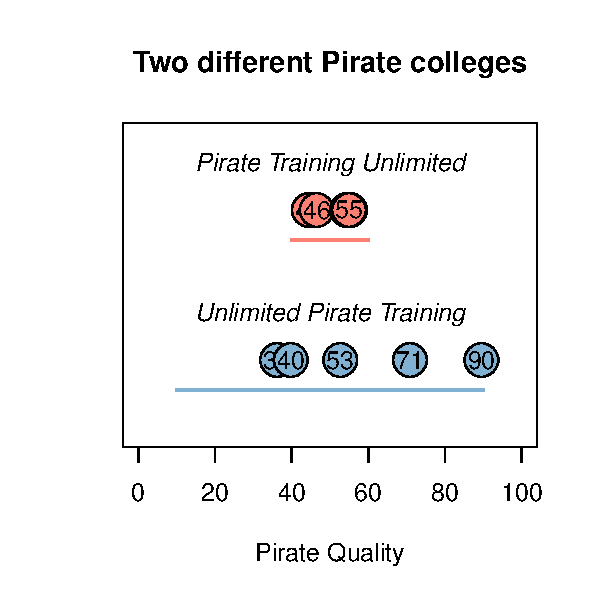
\includegraphics[width=\maxwidth]{figure/unnamed-chunk-32-1} 

\end{knitrout}
\caption{Visual depiction of a scalar and vector. Deep shit. Wait until we get to matrices - you're going to lose it.}
\label{fig:scalarvector}
\end{tiny}
\end{marginfigure}

\subsection{Vectors}

Now let's move onto \textit{vectors}. A \textbf{vector} is just a combination of several scalars stored as a single object. For example, the numbers from one to ten could be a vector of length 10. The characters in the English alphabet could be a vector of length 26. Like scalars, vectors can be either numeric or character (but not both!).

There are many ways to create vectors in R. Here is a table of the most common ones:


\begin{center}
\begin{tabular}{ |l|l|l| }
 \hline
 \multicolumn{1}{|c|}{\textbf{Function}} & \multicolumn{1}{|c|}{\textbf{Example}} & \multicolumn{1}{|c|}{\textbf{Result}} \\ \hline
\texttt{c(a, b)} & \texttt{c(1, 5, 9)} & [1, 5, 9] \\
\texttt{a:b} & \texttt{5:10} & [5, 6, 7, 8, 9, 10]\\
\texttt{seq(from, to, by, length.out)} &  \texttt{seq(from = 0, to = 6, by = 2)} & [0, 2, 4, 6] \\
\texttt{rep(x, times, each, length.out)} & \texttt{rep(c(1, 5), times = 2, each = 2)} & [1, 1, 5, 5, 1, 1, 5, 5]

\\
 \hline
\end{tabular}
\end{center}

Let's go through each function in detail:



\vspace{5mm} %5mm vertical space
\noindent
\setlength{\fboxrule}{1.5pt}
\fbox{
\parbox{\textwidth}{

\newfun{c(a, b, c, ...)}\index{c()}

\hline

\begin{description}

  \item[\tt{a, b, c, ...}] \hfill \\
      One or more objects to be combined into a vector
\end{description}

}
}
\vspace{5mm} %5mm vertical space

The simplest way to create a vector is with the \texttt{c()} function. The c here stands for concatenate, which means "bring them together". When using c(), place a comma in between the objects (scalers or vectors) you want to combine:

Let's use the \texttt{c()} function to create a vector called \texttt{my.vec} containing the integers from 1 to 5.

\begin{knitrout}
\definecolor{shadecolor}{rgb}{0.969, 0.969, 0.969}\color{fgcolor}\begin{kframe}
\begin{alltt}
\hlstd{my.vec} \hlkwb{<-} \hlkwd{c}\hlstd{(}\hlnum{1}\hlstd{,} \hlnum{2}\hlstd{,} \hlnum{3}\hlstd{,} \hlnum{4}\hlstd{,} \hlnum{5}\hlstd{)}
\end{alltt}
\end{kframe}
\end{knitrout}

Let's look at the object by evaluating it in the console:

\begin{knitrout}
\definecolor{shadecolor}{rgb}{0.969, 0.969, 0.969}\color{fgcolor}\begin{kframe}
\begin{alltt}
\hlstd{my.vec}
\end{alltt}
\begin{verbatim}
## [1] 1 2 3 4 5
\end{verbatim}
\end{kframe}
\end{knitrout}

As you can see, R has stored all 5 numbers in the object \texttt{my.vec}. Thanks R!


\marginnote{You can also create longer vectors by combining vectors you have already defined. Let's create a vector of the numbers from 1 to 10 by first generating a vector \texttt{a} from 1 to 5, and a vector \texttt{b} from 6 to 10 then combine them into a single vector \texttt{c}:}

\begin{marginfigure}

\begin{knitrout}
\definecolor{shadecolor}{rgb}{0.969, 0.969, 0.969}\color{fgcolor}\begin{kframe}
\begin{alltt}
\hlstd{one.to.five} \hlkwb{<-} \hlkwd{c}\hlstd{(}\hlnum{1}\hlstd{,} \hlnum{2}\hlstd{,} \hlnum{3}\hlstd{,} \hlnum{4}\hlstd{,} \hlnum{5}\hlstd{)}
\hlstd{six.to.ten} \hlkwb{<-} \hlkwd{c}\hlstd{(}\hlnum{6}\hlstd{,} \hlnum{7}\hlstd{,} \hlnum{8}\hlstd{,} \hlnum{9}\hlstd{,} \hlnum{10}\hlstd{)}
\hlstd{one.to.ten} \hlkwb{<-} \hlkwd{c}\hlstd{(a, b)}
\hlstd{one.to.ten}
\end{alltt}
\begin{verbatim}
## [1] 100.00   3.14
\end{verbatim}
\end{kframe}
\end{knitrout}

\end{marginfigure}

You can also create character vectors by using the \texttt{c()} function to combine character scalers. Here are some examples of character vectors:

\begin{knitrout}
\definecolor{shadecolor}{rgb}{0.969, 0.969, 0.969}\color{fgcolor}\begin{kframe}
\begin{alltt}
\hlstd{str.vec1} \hlkwb{<-} \hlkwd{c}\hlstd{(}\hlstr{"I"}\hlstd{,} \hlstr{"don't"}\hlstd{,} \hlstr{"like"}\hlstd{,} \hlstr{"Android"}\hlstd{,} \hlstr{"swords"}\hlstd{)}
\hlstd{str.vec2} \hlkwb{<-} \hlkwd{c}\hlstd{(}\hlstr{"this"}\hlstd{,} \hlstr{"is"}\hlstd{,} \hlstr{"not"}\hlstd{,} \hlstr{"a"}\hlstd{,} \hlstr{"pipe"}\hlstd{)}
\end{alltt}
\end{kframe}
\end{knitrout}

\subsection{Vectors contain either numbers or characters, not both!}

A vector can only contain one type of scalar: either numeric or character. If you try to create a vector with numeric and character scalars, then R will convert \textit{all} of the numeric scalars to characters.

\begin{knitrout}
\definecolor{shadecolor}{rgb}{0.969, 0.969, 0.969}\color{fgcolor}\begin{kframe}
\begin{alltt}
\hlstd{movie} \hlkwb{<-} \hlstr{"Pirates of the Carribean"}
\hlstd{revenue} \hlkwb{<-} \hlnum{634954111}
\hlkwd{c}\hlstd{(movie, revenue)} \hlcom{# Result is a string vector}
\end{alltt}
\begin{verbatim}
## [1] "Pirates of the Carribean" "634954111"
\end{verbatim}
\end{kframe}
\end{knitrout}

\section{Generating numeric vectors}

While the c() operator is the most straightforward way to create a vector, it's also one of the most tedious. Let's say you wanted to create a vector of all integers from 1 to 100. You definitely don't want to have to type all the numbers into a c() operator. Instead, R has many simple built-in functions for generating numeric vectors. Let's start with three of them: \texttt{a:b}, \texttt{seq()}, and \texttt{rep()}:

\subsection{a:b}

The \texttt{a:b} function creates a vector of numbers from the starting point a to the ending point b in steps of 1. You can go forwards or backwards depending on which number is larger.

\marginnote{\center{\Huge{a:b}}}

\vspace{5mm} %5mm vertical space
\noindent
\setlength{\fboxrule}{1.5pt}
\fbox{
\parbox{\textwidth}{

\newfun{a:b}\index{a:b}

\hline

\begin{description}

  \item[\tt{a}] \hfill \\
      The start of the sequence
  \item[\tt{b}] \hfill \\
      The end of the sequence
\end{description}

}
}
\vspace{5mm} %5mm vertical space

Here are some examples of the \texttt{a:b} function in action:


\begin{knitrout}
\definecolor{shadecolor}{rgb}{0.969, 0.969, 0.969}\color{fgcolor}\begin{kframe}
\begin{alltt}
\hlnum{1}\hlopt{:}\hlnum{10} \hlcom{# 1 to 10}
\end{alltt}
\begin{verbatim}
##  [1]  1  2  3  4  5  6  7  8  9 10
\end{verbatim}
\begin{alltt}
\hlnum{10}\hlopt{:}\hlnum{1} \hlcom{# 10 to 1}
\end{alltt}
\begin{verbatim}
##  [1] 10  9  8  7  6  5  4  3  2  1
\end{verbatim}
\begin{alltt}
\hlnum{20.1}\hlopt{:}\hlnum{30.1} \hlcom{# From 20.1 to 30.1}
\end{alltt}
\begin{verbatim}
##  [1] 20.1 21.1 22.1 23.1 24.1 25.1 26.1 27.1 28.1 29.1 30.1
\end{verbatim}
\end{kframe}
\end{knitrout}


\subsection{seq(from, to, by, length.out)}

The \texttt{seq()} function is a more flexible version of \texttt{a:b}. Like \texttt{a:b}, \texttt{seq()} allows you to create a sequence from a starting number to an ending number. However, with \texttt{seq()}, you can specify either the size of the steps between numbers, or the total length of the sequence:

\marginnote{\center{\Large{seq(from, to, by, length.out)}}}

\vspace{5mm} %5mm vertical space
\noindent
\setlength{\fboxrule}{1.5pt}
\fbox{
\parbox{\textwidth}{

\newfun{seq(from, to, by)}\index{seq()}

\hline

\begin{description}

  \item[\tt{from}] \hfill \\
      The start of the sequence
  \item[\tt{to}] \hfill \\
      The end of the sequence
  \item[\tt{by}] \hfill \\
      The step-size of the sequence \\
  \item[\tt{length.out}] \hfill \\
      The desired length of the final sequence (only use if you don't specify \texttt{by})
\end{description}

}
}
\vspace{5mm} %5mm vertical space

\marginnote{\textbf{seq(from, to, by)} - Creates a sequence between two numbers in steps that you specify. \\ \texttt{from}: The starting value \\ \texttt{to}: The ending value \\ \texttt{by}: The step size between \texttt{begin} and \texttt{end}}

The \texttt{seq()} function has two new arguments \textt{by} and \texttt{length.out}.

If you use the \texttt{by} argument, the sequence will be in steps of the input to the \texttt{by} argument:


\begin{knitrout}
\definecolor{shadecolor}{rgb}{0.969, 0.969, 0.969}\color{fgcolor}\begin{kframe}
\begin{alltt}
\hlkwd{seq}\hlstd{(}\hlkwc{from} \hlstd{=} \hlnum{1}\hlstd{,} \hlkwc{to} \hlstd{=} \hlnum{10}\hlstd{,} \hlkwc{by} \hlstd{=} \hlnum{1}\hlstd{)}
\end{alltt}
\begin{verbatim}
##  [1]  1  2  3  4  5  6  7  8  9 10
\end{verbatim}
\begin{alltt}
\hlkwd{seq}\hlstd{(}\hlkwc{from} \hlstd{=} \hlnum{0}\hlstd{,} \hlkwc{to} \hlstd{=} \hlnum{100}\hlstd{,} \hlkwc{by} \hlstd{=} \hlnum{10}\hlstd{)}
\end{alltt}
\begin{verbatim}
##  [1]   0  10  20  30  40  50  60  70  80  90 100
\end{verbatim}
\begin{alltt}
\hlkwd{seq}\hlstd{(}\hlkwc{from} \hlstd{=} \hlnum{20}\hlstd{,} \hlkwc{to} \hlstd{=} \hlnum{0}\hlstd{,} \hlkwc{by} \hlstd{=} \hlopt{-}\hlnum{2}\hlstd{)}
\end{alltt}
\begin{verbatim}
##  [1] 20 18 16 14 12 10  8  6  4  2  0
\end{verbatim}
\end{kframe}
\end{knitrout}


If you use the \texttt{length.out} argument, the sequence will have length equal to the input of \texttt{length.out}.

\begin{knitrout}
\definecolor{shadecolor}{rgb}{0.969, 0.969, 0.969}\color{fgcolor}\begin{kframe}
\begin{alltt}
\hlkwd{seq}\hlstd{(}\hlkwc{from} \hlstd{=} \hlnum{0}\hlstd{,} \hlkwc{to} \hlstd{=} \hlnum{100}\hlstd{,} \hlkwc{length.out} \hlstd{=} \hlnum{11}\hlstd{)}
\end{alltt}
\begin{verbatim}
##  [1]   0  10  20  30  40  50  60  70  80  90 100
\end{verbatim}
\begin{alltt}
\hlkwd{seq}\hlstd{(}\hlkwc{from} \hlstd{=} \hlnum{0}\hlstd{,} \hlkwc{to} \hlstd{=} \hlnum{100}\hlstd{,} \hlkwc{length.out} \hlstd{=} \hlnum{5}\hlstd{)}
\end{alltt}
\begin{verbatim}
## [1]   0  25  50  75 100
\end{verbatim}
\begin{alltt}
\hlkwd{seq}\hlstd{(}\hlkwc{from} \hlstd{=} \hlnum{0}\hlstd{,} \hlkwc{to} \hlstd{=} \hlnum{100}\hlstd{,} \hlkwc{length.out} \hlstd{=} \hlnum{2}\hlstd{)}
\end{alltt}
\begin{verbatim}
## [1]   0 100
\end{verbatim}
\end{kframe}
\end{knitrout}

\subsection{rep(x, times, each)}

The \texttt{rep()} function rep allows you to repeat a number (or vector) a specified number of times.

\vspace{5mm} %5mm vertical space
\noindent
\setlength{\fboxrule}{1.5pt}
\fbox{
\parbox{\textwidth}{

\newfun{rep(x, times, each)}\index{rep()}

\hline

\begin{description}

  \item[\tt{x}] \hfill \\
      A scaler or vector of values to repeat
  \item[\tt{times}] \hfill \\
      The number of times to repeat the sequence
  \item[\tt{each}] \hfill \\
      The number of times to repeat each value within the sequence \\
  \item[\tt{length.out} (optional)] \hfill \\
      The desired length of the final sequence \\
\end{description}

}
}
\vspace{5mm} %5mm vertical space

\marginnote{\textbf{rep(x, times, each)} - Repeats the numbers in x in a manner you specify \\ \texttt{times}: The number of times the vector should be repeated \\ \texttt{each}: The number of times you want to repeat each element in the vector.}

For example, let's say you are are getting a batch of 10 new pirates on your ship, and you need to assign each of them to one of three jobs. To help you, you could use a vector with the numbers 1, 2, 3, 1, 2, 3, etc.. Let's create this vector using \texttt{rep()}


\begin{knitrout}
\definecolor{shadecolor}{rgb}{0.969, 0.969, 0.969}\color{fgcolor}\begin{kframe}
\begin{alltt}
\hlstd{pirate.jobs.num} \hlkwb{<-} \hlkwd{rep}\hlstd{(}\hlkwc{x} \hlstd{=} \hlnum{1}\hlopt{:}\hlnum{3}\hlstd{,} \hlkwc{length.out} \hlstd{=} \hlnum{10}\hlstd{)}
\end{alltt}
\end{kframe}
\end{knitrout}


You can also use \texttt{rep()} to repeat vectors of character vectors. Let's repeat the previous example, but instead of using the numbers 1, 2, 3, we'll use the names of the actual jobs

\begin{knitrout}
\definecolor{shadecolor}{rgb}{0.969, 0.969, 0.969}\color{fgcolor}\begin{kframe}
\begin{alltt}
\hlstd{pirate.jobs.char} \hlkwb{<-} \hlkwd{rep}\hlstd{(}\hlkwc{x} \hlstd{=} \hlkwd{c}\hlstd{(}\hlstr{"Deck Swabber"}\hlstd{,} \hlstr{"Parrot Groomer"}\hlstd{,} \hlstr{"App Developer"}\hlstd{),}
                        \hlkwc{length.out} \hlstd{=} \hlnum{10}\hlstd{)}
\hlstd{pirate.jobs.char}
\end{alltt}
\begin{verbatim}
##  [1] "Deck Swabber"   "Parrot Groomer" "App Developer"  "Deck Swabber"  
##  [5] "Parrot Groomer" "App Developer"  "Deck Swabber"   "Parrot Groomer"
##  [9] "App Developer"  "Deck Swabber"
\end{verbatim}
\end{kframe}
\end{knitrout}

The each argument allows you to repeat each element in the original vector within each repetition. Wow, that was a confusing sentence. Let me just show you:

\begin{knitrout}
\definecolor{shadecolor}{rgb}{0.969, 0.969, 0.969}\color{fgcolor}\begin{kframe}
\begin{alltt}
\hlkwd{rep}\hlstd{(}\hlkwc{x} \hlstd{=} \hlnum{1}\hlopt{:}\hlnum{4}\hlstd{,} \hlkwc{each} \hlstd{=} \hlnum{2}\hlstd{)}
\end{alltt}
\begin{verbatim}
## [1] 1 1 2 2 3 3 4 4
\end{verbatim}
\begin{alltt}
\hlkwd{rep}\hlstd{(}\hlkwc{x} \hlstd{=} \hlkwd{c}\hlstd{(}\hlstr{"a"}\hlstd{,} \hlstr{"b"}\hlstd{),} \hlkwc{each} \hlstd{=} \hlnum{3}\hlstd{,} \hlkwc{times} \hlstd{=} \hlnum{2}\hlstd{)}
\end{alltt}
\begin{verbatim}
##  [1] "a" "a" "a" "b" "b" "b" "a" "a" "a" "b" "b" "b"
\end{verbatim}
\end{kframe}
\end{knitrout}

\subsection{length()}

\marginnote{\center{\Huge{length(x)}}}

Once you have a vector, you may want to know how long it is. Don't stare at your computer screen and count the elements one by one! Instead, use \texttt{length()} function:

\begin{knitrout}
\definecolor{shadecolor}{rgb}{0.969, 0.969, 0.969}\color{fgcolor}\begin{kframe}
\begin{alltt}
\hlkwd{length}\hlstd{(}\hlnum{1}\hlopt{:}\hlnum{10}\hlstd{)}
\end{alltt}
\begin{verbatim}
## [1] 10
\end{verbatim}
\begin{alltt}
\hlkwd{length}\hlstd{(}\hlkwd{seq}\hlstd{(}\hlkwc{from} \hlstd{=} \hlnum{1}\hlstd{,} \hlkwc{to} \hlstd{=} \hlnum{100}\hlstd{,} \hlkwc{length.out} \hlstd{=} \hlnum{20}\hlstd{))}
\end{alltt}
\begin{verbatim}
## [1] 20
\end{verbatim}
\begin{alltt}
\hlkwd{length}\hlstd{(}\hlkwd{c}\hlstd{(}\hlstr{"This"}\hlstd{,} \hlstr{"character"}\hlstd{,} \hlstr{"vector"}\hlstd{,} \hlstr{"has"}\hlstd{,} \hlstr{"six"}\hlstd{,} \hlstr{"elements."}\hlstd{))}
\end{alltt}
\begin{verbatim}
## [1] 6
\end{verbatim}
\begin{alltt}
\hlkwd{length}\hlstd{(}\hlstr{"This character scaler has just one element."}\hlstd{)}
\end{alltt}
\begin{verbatim}
## [1] 1
\end{verbatim}
\end{kframe}
\end{knitrout}



\section{Test your R might!}


\begin{enumerate}

\item 2015 was a good year for pirate booty - your ship collected 100,800 gold coins. Create an object called \texttt{gold.in.2015} and assign the correct value to it.

\item Oops, during the last inspection we discovered that one of your pirates ``Skippy McGee" hid 800 gold coins in his underwear. Go ahead and add those gold coins to the object \texttt{gold.in.2015}. Next, create a character object called \texttt{plank.list} with the name of the pirate thief.

\item Look at the code below. What will R return after the third line? Make a prediction, then test the code yourself.

\begin{knitrout}
\definecolor{shadecolor}{rgb}{0.969, 0.969, 0.969}\color{fgcolor}\begin{kframe}
\begin{alltt}
\hlstd{a} \hlkwb{<-} \hlnum{10}
\hlstd{a} \hlopt{+} \hlnum{10}
\hlstd{a}
\end{alltt}
\end{kframe}
\end{knitrout}

\item Create the vector [1, 2, 3, 4, 5, 6, 7, 8, 9, 10] in three ways: once using \texttt{c()}, once using \texttt{a:b}, and once using \texttt{seq()}.

\item Create the vector [2.1, 4.1, 6.1, 8.1] in two ways, once using \texttt{c()} and once using \texttt{seq()}

\item Create the vector [0, 5, 10, 15] in 3 ways: using \texttt{c()}, \texttt{seq()} with a \texttt{by} argument, and \texttt{seq()} with a \texttt{length.out} argument.

\item Create the vector [101, 102, 103, 200, 205, 210, 1000, 1100, 1200] using a combination of the \texttt{c()} and \texttt{seq()} functions

\item A new batch of 100 pirates are boarding your ship and need new swords. You have 10 scimitars, 40 broadswords, and 50 cutlasses that you need to distribute evenly to the 100 pirates as they board. Create a vector of length 100 where there is 1 scimitar, 4 broadswords, and 5 cutlasses in each group of 10. That is, in the first 10 elements there should be exactly 1 scimitar, 4 broadswords and 5 cutlasses. The next 10 elements should also have the same number of each sword (and so on).

\item Create an object called \texttt{overboard} containing the text ``NNNNNNOOOOOOoooooo!!!!!!'' as a vector of length 24 using the \texttt{rep()} function.


\end{enumerate}


\section{Additional Tips}


\begin{enumerate}

  \item If you want to run a single line of code, you don't need to highlight anything. Instead, click on the line you want to run and use the "Run" hot-key (\texttt{command + enter} on Mac), or click the ``Run" button. R will execute just that line - and automatically move the cursor to the next line. To run the next line, just hit the hot-key again. This is a great way to test your code line-by-line.

  \item To get more tips on how good coding techniques, check out the R style guide at http://adv-r.had.co.nz/Style.html. For great blog articles on R, check out http://www.r-bloggers.com/

  \item If you need to enter a lot of numeric data into R by hand you might want to use the \texttt{scan()} function. This function allows you to easily enter data using 10-key typing on a number pad. To do this, run the code \texttt{scan()} and then enter the data number by number. When you are finished, R will then print the appropriate code to store the data into a vector.

  \item You can run several lines of code in one line by separating the code with the ; key. For example, the following two chunks of code are the same:

\begin{knitrout}
\definecolor{shadecolor}{rgb}{0.969, 0.969, 0.969}\color{fgcolor}\begin{kframe}
\begin{alltt}
\hlstd{a} \hlkwb{<-} \hlnum{1}
\hlstd{b} \hlkwb{<-} \hlnum{14}
\hlstd{c} \hlkwb{<-} \hlnum{67}
\end{alltt}
\end{kframe}
\end{knitrout}

\begin{knitrout}
\definecolor{shadecolor}{rgb}{0.969, 0.969, 0.969}\color{fgcolor}\begin{kframe}
\begin{alltt}
\hlstd{a} \hlkwb{<-} \hlnum{1} \hlstd{; b} \hlkwb{<-} \hlnum{14} \hlstd{; c} \hlkwb{<-} \hlnum{67}
\end{alltt}
\end{kframe}
\end{knitrout}


  However, I recommend you use the ; key sparingly (if at all). If you get in the habit of trying to cram several lines of code in one line, your code will get cluttered and difficult to understand.

\end{enumerate}



%----------------------------------------------------------------------------------------
%	CHAPTER 3
%----------------------------------------------------------------------------------------

\chapter{3: Vector arithmetic and descriptive statistics}
\label{ch:3}

\textit{Chapter Goals}

\begin{enumerate}
  \item Do simple math operations on vectors
  \item Learn functions for basic descriptive statistics: mean(), median(), sd(), var(), min(), max()
\end{enumerate}


\section{Arithmetic operations on vectors}

So far, you know how to do You can do basic arithmetic operations like + (addition), - (subtraction), and * (multiplication) on scalars. Thankfully, R makes it just as easy to do arithmetic operations on numeric vectors.

\subsection{Basic math with vectors and scalers}

If you do an operation on a vector with a scalar, R will apply the scalar to each element in the vector. For example, if you want to add 100 to every element in a vector, you can just treat them both like scalers. Let's create a vector with the integers from 1 to 10 and add 100 to each element:


\begin{knitrout}
\definecolor{shadecolor}{rgb}{0.969, 0.969, 0.969}\color{fgcolor}\begin{kframe}
\begin{alltt}
\hlstd{a} \hlkwb{<-} \hlnum{1}\hlopt{:}\hlnum{10}
\hlstd{a} \hlopt{+} \hlnum{100}
\end{alltt}
\begin{verbatim}
##  [1] 101 102 103 104 105 106 107 108 109 110
\end{verbatim}
\end{kframe}
\end{knitrout}


The result is a vector where the first element is 1 + 100, the second element is 2 + 100 (etc.). Of course, this doesn't only work with addition...oh no. Let's try division, multiplication, and exponents:

\begin{knitrout}
\definecolor{shadecolor}{rgb}{0.969, 0.969, 0.969}\color{fgcolor}\begin{kframe}
\begin{alltt}
\hlstd{a} \hlkwb{<-} \hlnum{1}\hlopt{:}\hlnum{10}
\hlstd{a} \hlopt{/} \hlnum{100}
\end{alltt}
\begin{verbatim}
##  [1] 0.01 0.02 0.03 0.04 0.05 0.06 0.07 0.08 0.09 0.10
\end{verbatim}
\begin{alltt}
\hlstd{a} \hlopt{^} \hlnum{2}
\end{alltt}
\begin{verbatim}
##  [1]   1   4   9  16  25  36  49  64  81 100
\end{verbatim}
\end{kframe}
\end{knitrout}

Again, if you perform an algebraic operation on a vector with a scaler, R will just apply the operation to every element in the vector.

\subsection{Basic math with multiple vectors}

What if you want to do some operation on two vectors? For example, let's say you had a bake sale on your ship where 5 pirates sold both pies and cookies. You could record the total number of pies and cookies sold in two vectors:

\begin{knitrout}
\definecolor{shadecolor}{rgb}{0.969, 0.969, 0.969}\color{fgcolor}\begin{kframe}
\begin{alltt}
\hlstd{pies} \hlkwb{<-} \hlkwd{c}\hlstd{(}\hlnum{3}\hlstd{,} \hlnum{6}\hlstd{,} \hlnum{2}\hlstd{,} \hlnum{10}\hlstd{,} \hlnum{4}\hlstd{)}
\hlstd{cookies} \hlkwb{<-} \hlkwd{c}\hlstd{(}\hlnum{70}\hlstd{,} \hlnum{40}\hlstd{,} \hlnum{40}\hlstd{,} \hlnum{200}\hlstd{,} \hlnum{60}\hlstd{)}
\end{alltt}
\end{kframe}
\end{knitrout}

Now, let's say you want to know how many total items each pirate sold. You can do this by just adding the two vectors:

\begin{knitrout}
\definecolor{shadecolor}{rgb}{0.969, 0.969, 0.969}\color{fgcolor}\begin{kframe}
\begin{alltt}
\hlstd{total} \hlkwb{<-} \hlstd{pies} \hlopt{+} \hlstd{cookies}
\hlstd{total}
\end{alltt}
\begin{verbatim}
## [1]  73  46  42 210  64
\end{verbatim}
\end{kframe}
\end{knitrout}


\marginnote{If you try to do basic operations on two vectors of unequal length, R will try to increase the length of the shorter vector by repeating it. For example, if you try to add [1, 2] with [1, 2, 3, 4, 5, 6], you get the following result}

\begin{marginfigure}

\begin{knitrout}
\definecolor{shadecolor}{rgb}{0.969, 0.969, 0.969}\color{fgcolor}\begin{kframe}
\begin{alltt}
\hlstd{a} \hlkwb{<-} \hlkwd{c}\hlstd{(}\hlnum{0}\hlstd{,} \hlnum{100}\hlstd{)}
\hlstd{b} \hlkwb{<-} \hlkwd{c}\hlstd{(}\hlnum{1}\hlstd{,} \hlnum{2}\hlstd{,} \hlnum{3}\hlstd{,} \hlnum{4}\hlstd{,} \hlnum{5}\hlstd{,} \hlnum{6}\hlstd{)}
\hlstd{a} \hlopt{+} \hlstd{b}
\end{alltt}
\begin{verbatim}
## [1]   1 102   3 104   5 106
\end{verbatim}
\end{kframe}
\end{knitrout}

\end{marginfigure}

As this example shows, if you do an operation on two vectors, R will try to apply the operation between the vectors by each item. For example, if you add two vectors of equal length (like we did above), R will create a new vector of the same length where each element is the sum of the elements in the previous vector.

Let's create two vectors a and b where each vector contains the integers from 1 to 5. We'll then create two new vectors \texttt{ab.sum}, the sum of the two vectors and \texttt{ab.diff}, the difference of the two vectors, and \texttt{ab.prod}, the product of the two vectors:


\begin{knitrout}
\definecolor{shadecolor}{rgb}{0.969, 0.969, 0.969}\color{fgcolor}\begin{kframe}
\begin{alltt}
\hlstd{a} \hlkwb{<-} \hlnum{1}\hlopt{:}\hlnum{5}
\hlstd{b} \hlkwb{<-} \hlnum{1}\hlopt{:}\hlnum{5}

\hlstd{ab.sum} \hlkwb{<-} \hlstd{a} \hlopt{+} \hlstd{b}
\hlstd{ab.diff} \hlkwb{<-} \hlstd{a} \hlopt{-} \hlstd{b}
\hlstd{ab.prod} \hlkwb{<-} \hlstd{a} \hlopt{*} \hlstd{b}

\hlstd{ab.sum}
\end{alltt}
\begin{verbatim}
## [1]  2  4  6  8 10
\end{verbatim}
\begin{alltt}
\hlstd{ab.diff}
\end{alltt}
\begin{verbatim}
## [1] 0 0 0 0 0
\end{verbatim}
\begin{alltt}
\hlstd{ab.prod}
\end{alltt}
\begin{verbatim}
## [1]  1  4  9 16 25
\end{verbatim}
\end{kframe}
\end{knitrout}

\section{Summary statistics for Continuous data}

Ok, now that we can generate some data, let's learn the basic descriptive statistics functions. We'll focus on the most common ones for numerical analyses. Each of the following functions takes a vector as an argument, and returns a scalar as a result.


\vspace{5mm} %5mm vertical space
\noindent
\setlength{\fboxrule}{1.5pt}
\fbox{
\parbox{\textwidth}{

\newfun{Common Descriptive Statistics}

\hline

\begin{description}

\item[\tt{mean(x)}] \hfill \\
    The arithmetic mean of a vector x
\item[\tt{median(x)}] \hfill \\
    The median of a vector x. 50\% of the data should be less than \texttt{median(x)} and 50\% should be greater than \texttt{median(x)}.
\item[\tt{sd(x), var(x)}] \hfill \\
    The standard deviation and variance of a vector x.
\item[\tt{min(x), max(x)}] \hfill \\
    The minimum and maximum values of a vector x
\item[\tt{quantile(x, p)}] \hfill \\
    The pth sample quantile of a vector x. For example, \texttt{quantile(x, .2)} will tell you the value at which 20\% of cases are less than x. The function \texttt{quantile(x, .5)} is identical to \texttt{median(x)}
\item[\tt{summary(x)}] \hfill \\
  Shows you several descriptive statistics of a vector x, including \texttt{min(x)}, \texttt{max(x)}, \texttt{median(x)}, \texttt{mean(x)}

\end{description}

}
}
\vspace{5mm} %5mm vertical space


Let's calculate some descriptive statistics from some pirate related data. I'll create a vector called \texttt{data} that contains the number of tattoos from 10 random pirates.

\begin{knitrout}
\definecolor{shadecolor}{rgb}{0.969, 0.969, 0.969}\color{fgcolor}\begin{kframe}
\begin{alltt}
\hlstd{tattoos} \hlkwb{<-} \hlkwd{c}\hlstd{(}\hlnum{4}\hlstd{,} \hlnum{50}\hlstd{,} \hlnum{2}\hlstd{,} \hlnum{39}\hlstd{,} \hlnum{4}\hlstd{,} \hlnum{20}\hlstd{,} \hlnum{4}\hlstd{,} \hlnum{8}\hlstd{,} \hlnum{10}\hlstd{,} \hlnum{100}\hlstd{)}
\end{alltt}
\end{kframe}
\end{knitrout}

Now, we can calculate several descriptive statistics on this vector by using the summary statistics functions:

\begin{knitrout}
\definecolor{shadecolor}{rgb}{0.969, 0.969, 0.969}\color{fgcolor}\begin{kframe}
\begin{alltt}
\hlkwd{mean}\hlstd{(tattoos)}
\end{alltt}
\begin{verbatim}
## [1] 24.1
\end{verbatim}
\begin{alltt}
\hlkwd{median}\hlstd{(tattoos)}
\end{alltt}
\begin{verbatim}
## [1] 9
\end{verbatim}
\begin{alltt}
\hlkwd{sd}\hlstd{(tattoos)}
\end{alltt}
\begin{verbatim}
## [1] 31.32074
\end{verbatim}
\begin{alltt}
\hlkwd{min}\hlstd{(tattoos)}
\end{alltt}
\begin{verbatim}
## [1] 2
\end{verbatim}
\begin{alltt}
\hlkwd{max}\hlstd{(tattoos)}
\end{alltt}
\begin{verbatim}
## [1] 100
\end{verbatim}
\end{kframe}
\end{knitrout}

\subsection{Watch out for NA values!}

One important point about the descriptive statistics functions is that most (if not all) of them as a default will freak out if there is a missing (NA) value in the data. For example, the following code will return NA as a result because there is an NA value in the data vector:

\marginnote{Include the argument \textt{na.rm = T} to ignore missing (NA) values when calculating a descriptive statistic.}

\begin{knitrout}
\definecolor{shadecolor}{rgb}{0.969, 0.969, 0.969}\color{fgcolor}\begin{kframe}
\begin{alltt}
\hlkwd{mean}\hlstd{(}\hlkwd{c}\hlstd{(}\hlnum{1}\hlstd{,} \hlnum{5}\hlstd{,} \hlnum{NA}\hlstd{,} \hlnum{2}\hlstd{))}
\end{alltt}
\begin{verbatim}
## [1] NA
\end{verbatim}
\end{kframe}
\end{knitrout}

To tell a descriptive statistic function to ignore missing (NA) values, include the argument \texttt{na.rm = T} in the function:

\begin{knitrout}
\definecolor{shadecolor}{rgb}{0.969, 0.969, 0.969}\color{fgcolor}\begin{kframe}
\begin{alltt}
\hlkwd{mean}\hlstd{(}\hlkwd{c}\hlstd{(}\hlnum{1}\hlstd{,} \hlnum{5}\hlstd{,} \hlnum{NA}\hlstd{,} \hlnum{2}\hlstd{),} \hlkwc{na.rm} \hlstd{= T)}
\end{alltt}
\begin{verbatim}
## [1] 2.666667
\end{verbatim}
\end{kframe}
\end{knitrout}

Now, the function will ignore NA and calculate the mean of the non-missing values. While this may seem trivial now (why did we include an NA value in the vector if we wanted to ignore it?!), it will be become very important when we apply the function to large existing datasets that may contain missing values.


If you want to get many summary statistics from a vector, you can use the \textbf{summary()} function which gives you several key statistics:

\begin{footnotesize}
\begin{knitrout}
\definecolor{shadecolor}{rgb}{0.969, 0.969, 0.969}\color{fgcolor}\begin{kframe}
\begin{alltt}
\hlkwd{summary}\hlstd{(tattoos)}
\end{alltt}
\begin{verbatim}
##    Min. 1st Qu.  Median    Mean 3rd Qu.    Max. 
##    2.00    4.00    9.00   24.10   34.25  100.00
\end{verbatim}
\end{kframe}
\end{knitrout}
\end{footnotesize}



\subsection{Other helpful vector functions}

Here are some other functions that you will find useful when managing numeric vectors:


\vspace{5mm} %5mm vertical space
\noindent
\setlength{\fboxrule}{1.5pt}
\fbox{
\parbox{\textwidth}{

\newfun{Other helpful numeric functions}

\hline

\begin{description}

\item[\tt{round(x, digits)}] \hfill \\
    Round values in a vector (or scaler) x to a certain number of digits.
\item[\tt{ceiling(x), floor(x)}] \hfill \\
   Round a number to the next largest integer with \texttt{ceiling(x)} or down to the next lowest integer with \texttt{floor(x)}.
\item[\tt{x \%\% y}] \hfill \\
    Modular arithmetic (i.e.; x mod y). You can interpret \texttt{x \%\% y} as ``What is the remainder after dividing x by y?" For example, \texttt{10 \%\% 3} equals 1 because 3 times 3 is 9 (which leaves a remainder of 1).
\end{description}

}
}
\vspace{5mm} %5mm vertical space

\subsection{Standardizing (z-score) variables}

During one of your morning strolls on your ship's deck, you see two pieces of paper with the titles: ``Mugs of Grogg'' and ``Climbing'' respectively. On each piece, you see the following numbers:

\begin{knitrout}
\definecolor{shadecolor}{rgb}{0.969, 0.969, 0.969}\color{fgcolor}\begin{kframe}
\begin{alltt}
\hlstd{grogg} \hlkwb{<-} \hlkwd{c}\hlstd{(}\hlnum{12}\hlstd{,} \hlnum{8}\hlstd{,} \hlnum{1}\hlstd{,} \hlnum{6}\hlstd{,} \hlnum{2}\hlstd{)}
\hlstd{climbing} \hlkwb{<-} \hlkwd{c}\hlstd{(}\hlnum{100}\hlstd{,} \hlnum{520}\hlstd{,} \hlnum{430}\hlstd{,} \hlnum{200}\hlstd{,} \hlnum{700}\hlstd{)}
\end{alltt}
\end{kframe}
\end{knitrout}

Now you know what was keeping you up last night: it turns out your crew of 5 pirates had two contests last night. In one, the pirates drank as many mugs of grogg as they could in 5 minutes. In the second, they saw how many feet of rope the pirate could climb in an hour. Now you're curious how well each pirate did and which performances were the most spectacular. But there's a problem: the scales of the numbers are very different. While the grogg numbers range from 1 to 12, the climbing numbers have a much larger range from 100 to 700. This makes it difficult to compare the two sets of numbers directly.

To solve this problem, we can use \textit{standardization}. Put simply, standardizing is a common method to put all vectors of numbers on a similar scale. Specifically, it requires subtracting the mean from a set of numbers, and then dividing the numbers by their standard deviation. Once you've standardized a set of numbers, you can interpret a value of x as being `x standard deviations away from the mean.'

Let's use standardization to create new vectors called \texttt{grogg.z} and \texttt{climbing.z}

\begin{knitrout}
\definecolor{shadecolor}{rgb}{0.969, 0.969, 0.969}\color{fgcolor}\begin{kframe}
\begin{alltt}
\hlstd{grogg.z} \hlkwb{<-} \hlstd{(grogg} \hlopt{-} \hlkwd{mean}\hlstd{(grogg))} \hlopt{/} \hlkwd{sd}\hlstd{(grogg)}
\hlstd{climbing.z} \hlkwb{<-} \hlstd{(climbing} \hlopt{-} \hlkwd{mean}\hlstd{(climbing))} \hlopt{/} \hlkwd{sd}\hlstd{(climbing)}
\end{alltt}
\end{kframe}
\end{knitrout}

Now let's look at the final results. To make them easier to read, I'll round them to 2 digits:

\begin{knitrout}
\definecolor{shadecolor}{rgb}{0.969, 0.969, 0.969}\color{fgcolor}\begin{kframe}
\begin{alltt}
\hlkwd{round}\hlstd{(grogg.z,} \hlnum{1}\hlstd{)}
\end{alltt}
\begin{verbatim}
## [1]  1.4  0.5 -1.1  0.0 -0.8
\end{verbatim}
\begin{alltt}
\hlkwd{round}\hlstd{(climbing.z,} \hlnum{1}\hlstd{)}
\end{alltt}
\begin{verbatim}
## [1] -1.2  0.5  0.2 -0.8  1.3
\end{verbatim}
\end{kframe}
\end{knitrout}

It looks like we we have two outstanding performances in particular. In the grogg drinking competition, the first pirate had a z-score of 1.4. We can interpret this by saying that this pirate drank 1.4 more standard deviations of mugs of grogg than the average pirate. In the climbing competition, the fifth pirate had a z-score of 1.3. Here, we would conclude that this pirate climbed 1.3 standard deviations more than the average pirate.


\begin{marginfigure}

Here's an easy function for standardization:

\begin{knitrout}
\definecolor{shadecolor}{rgb}{0.969, 0.969, 0.969}\color{fgcolor}\begin{kframe}
\begin{alltt}
\hlstd{standardize} \hlkwb{<-} \hlkwa{function}\hlstd{(}\hlkwc{x}\hlstd{) \{}

  \hlkwd{return}\hlstd{((x} \hlopt{-} \hlkwd{mean}\hlstd{(x))} \hlopt{/} \hlkwd{sd}\hlstd{(x))}

\hlstd{\}}
\end{alltt}
\end{kframe}
\end{knitrout}

\end{marginfigure}

But which pirate was the best on average across both events? To answer this, let's create a combined z-score for each pirate which calculates the average z-scores for each pirate by adding two performances and dividing by two. This will tell us, how good, on average, each pirate did relative to her fellow pirates.

\begin{knitrout}
\definecolor{shadecolor}{rgb}{0.969, 0.969, 0.969}\color{fgcolor}\begin{kframe}
\begin{alltt}
\hlstd{average.z} \hlkwb{<-} \hlstd{(grogg.z} \hlopt{+} \hlstd{(climbing.z))} \hlopt{/} \hlnum{2}
\end{alltt}
\end{kframe}
\end{knitrout}

Let's look at the result

\begin{knitrout}
\definecolor{shadecolor}{rgb}{0.969, 0.969, 0.969}\color{fgcolor}\begin{kframe}
\begin{alltt}
\hlkwd{round}\hlstd{(average.z,} \hlnum{1}\hlstd{)}
\end{alltt}
\begin{verbatim}
## [1]  0.1  0.5 -0.5 -0.4  0.2
\end{verbatim}
\end{kframe}
\end{knitrout}

The highest average z-score belongs to the second pirate who had an average z-score value of 0.5. The first and last pirates, who did well in one event, seemed to have done poorly in the other event.

Moral of the story: promote the pirate who can drink \textit{and} climb.


\section{Summary Statistics for Discrete data}

Next, we'll move on to common summary statistics for discrete data. Discrete data are those like gender, occupation, or favorite pirate movie that only allow for a finite (or at least, plausibly finite) set of responses.



\vspace{5mm} %5mm vertical space
\noindent
\setlength{\fboxrule}{1.5pt}
\fbox{
\parbox{\textwidth}{

\newfun{Discrete data summary statistics}

\hline

\begin{description}

\item[\tt{unique(x)}] \hfill \\
    Returns a vector of all unique values in the vector x.

\item[\tt{table(x)}] \hfill \\
  Returns a table showing all the unique values in the vector x as well as a count of each occurrence. By default, the \texttt{table()} function does NOT count NA values. To include a count of NA values, include the argument \texttt{exclude = NULL}


\end{description}

}
}
\vspace{5mm} %5mm vertical space

Let's start with two vectors of discrete data:

\begin{knitrout}
\definecolor{shadecolor}{rgb}{0.969, 0.969, 0.969}\color{fgcolor}\begin{kframe}
\begin{alltt}
\hlstd{vec} \hlkwb{<-} \hlkwd{c}\hlstd{(}\hlnum{1}\hlstd{,} \hlnum{1}\hlstd{,} \hlnum{1}\hlstd{,} \hlnum{5}\hlstd{,} \hlnum{1}\hlstd{,} \hlnum{1}\hlstd{,} \hlnum{10}\hlstd{,} \hlnum{10}\hlstd{,} \hlnum{10}\hlstd{)}
\hlstd{gender} \hlkwb{<-} \hlkwd{c}\hlstd{(}\hlstr{"M"}\hlstd{,} \hlstr{"M"}\hlstd{,} \hlstr{"F"}\hlstd{,} \hlstr{"F"}\hlstd{,} \hlstr{"F"}\hlstd{,} \hlstr{"M"}\hlstd{,} \hlstr{"F"}\hlstd{,} \hlstr{"M"}\hlstd{,} \hlstr{"F"}\hlstd{)}
\end{alltt}
\end{kframe}
\end{knitrout}


The function \texttt{unique(x)} will tell you all the unique values in the vector, but won't tell you anything about how often each value occurs.

\marginnote{\textbf{unique(x)}: Gives you all unique values in a vector, ignoring the number of times each value occurs.}

\begin{knitrout}
\definecolor{shadecolor}{rgb}{0.969, 0.969, 0.969}\color{fgcolor}\begin{kframe}
\begin{alltt}
\hlkwd{unique}\hlstd{(vec)}
\end{alltt}
\begin{verbatim}
## [1]  1  5 10
\end{verbatim}
\begin{alltt}
\hlkwd{unique}\hlstd{(gender)}
\end{alltt}
\begin{verbatim}
## [1] "M" "F"
\end{verbatim}
\end{kframe}
\end{knitrout}


The function \texttt{table()} does the same thing as \texttt{unique()}, but goes a step further in telling you how often each of the unique values occurs:

\marginnote{\textbf{table(x)}: Gives you all unique values in a vector and tells you how often each value occurs.}

\begin{knitrout}
\definecolor{shadecolor}{rgb}{0.969, 0.969, 0.969}\color{fgcolor}\begin{kframe}
\begin{alltt}
\hlkwd{table}\hlstd{(vec)}
\end{alltt}
\begin{verbatim}
## vec
##  1  5 10 
##  5  1  3
\end{verbatim}
\begin{alltt}
\hlkwd{table}\hlstd{(gender)}
\end{alltt}
\begin{verbatim}
## gender
## F M 
## 5 4
\end{verbatim}
\end{kframe}
\end{knitrout}

If you want to get percentages instead of counts, you can just divide the result of the \texttt{table()} function by the sum of the result:

\begin{knitrout}
\definecolor{shadecolor}{rgb}{0.969, 0.969, 0.969}\color{fgcolor}\begin{kframe}
\begin{alltt}
\hlkwd{table}\hlstd{(vec)} \hlopt{/} \hlkwd{sum}\hlstd{(}\hlkwd{table}\hlstd{(vec))}
\end{alltt}
\begin{verbatim}
## vec
##         1         5        10 
## 0.5555556 0.1111111 0.3333333
\end{verbatim}
\begin{alltt}
\hlkwd{table}\hlstd{(gender)} \hlopt{/} \hlkwd{sum}\hlstd{(}\hlkwd{table}\hlstd{(gender))}
\end{alltt}
\begin{verbatim}
## gender
##         F         M 
## 0.5555556 0.4444444
\end{verbatim}
\end{kframe}
\end{knitrout}




\subsection{Additional Tips}

\section{Test your R Might!}

\begin{enumerate}

\item Create a vector that shows the square root of the integers from 1 to 10.

\item Create a vector that shows the powers of 2 from 1 to 10. That is, the first element should be 2^1, the second element should be 2^2 (etc.)

Renata thinks that she finds more treasure when she's had a mug of grogg than when she doesn't. To test this, she recorded how much treasure she found over 7 days without drinking any grogg, and then did the same over 7 days while drinking grogg. Here are her results:

\begin{knitrout}
\definecolor{shadecolor}{rgb}{0.969, 0.969, 0.969}\color{fgcolor}\begin{kframe}
\begin{alltt}
\hlstd{grogg} \hlkwb{<-} \hlkwd{c}\hlstd{(}\hlnum{2}\hlstd{,} \hlnum{0}\hlstd{,} \hlnum{3}\hlstd{,} \hlnum{1}\hlstd{,} \hlnum{0}\hlstd{,} \hlnum{3}\hlstd{,} \hlnum{5}\hlstd{)}
\hlstd{nogrogg} \hlkwb{<-} \hlkwd{c}\hlstd{(}\hlnum{0}\hlstd{,} \hlnum{0}\hlstd{,} \hlnum{1}\hlstd{,} \hlnum{0}\hlstd{,} \hlnum{1}\hlstd{,} \hlnum{2}\hlstd{,} \hlnum{2}\hlstd{)}
\end{alltt}
\end{kframe}
\end{knitrout}

\item How much treasure did Renata find on average when drinking grogg? What about when she did not drink grogg?

\item Create a new vector called \texttt{difference} that shows how much more treasure Renata found while drinking grogg than when she didn't drink grogg.

\item What was the mean, median, and standard deviation of the difference?

\end{enumerate}





%----------------------------------------------------------------------------------------
%	CHAPTER 4
%----------------------------------------------------------------------------------------

\chapter{4: Indexing and comparing vectors}
\label{ch:4}


Chapter Goals:

\begin{enumerate}
  \item Use brackets [] and logical vectors to index vectors
  \item Combine indexing with descriptive statistics
  \item Learn indexing functions which(), sort()
  \item Vector discrete summary functions table() and unique()
  \item Set functions: intersect(), union(), setdiff(), %in%
\end{enumerate}


\section{Indexing vectors with brackets}

\marginnote{\textbf{Indexing with brackets [ ]} \\ To get the ith value of a vector called \texttt{vec}, use the bracket notation \textt{vec[i]}}

When we have a vector of data, we will frequently want to access specific values of a vector. These might be values in a specific location in the vector (i.e.; the fifth element) or based on some criteria (i.e.; all values greater than 0). For example, let's say we did a survey of  pirates and asked each pirate two questions: ``What is your favorite board game?'' and ``How long is your beard (in cm)?''. We can represent these data in two vectors:

\begin{footnotesize}
\begin{knitrout}
\definecolor{shadecolor}{rgb}{0.969, 0.969, 0.969}\color{fgcolor}\begin{kframe}
\begin{alltt}
\hlstd{fav.game} \hlkwb{<-} \hlkwd{c}\hlstd{(}\hlstr{"Pir of Catan"}\hlstd{,} \hlstr{"Pir of Catan"}\hlstd{,} \hlstr{"Piratopoly"}\hlstd{,}
              \hlstr{"Piratopoly"}\hlstd{,} \hlstr{"Pir of Catan"}\hlstd{)}

\hlstd{beard.length} \hlkwb{<-} \hlkwd{c}\hlstd{(}\hlnum{30}\hlstd{,} \hlnum{24}\hlstd{,} \hlnum{0}\hlstd{,} \hlnum{40}\hlstd{,} \hlnum{15}\hlstd{)}
\end{alltt}
\end{kframe}
\end{knitrout}
\end{footnotesize}


As you can see, we have two dominant board games here: Pirates of Catan and Piratopoly. Now, what if we wanted to calculate summary statistics, on beard length (like the mean, median, or standard deviation) separately for pirates whose favorite board game is Pirates of Catan and for those whose favorite game is Piratopoly? Unfortunately we can't simply do this by applying the summary statistic function to the \texttt{beard.length} vector. We need to find some way of telling R to \textit{index} the \texttt{beard.length} vector based on the different values of the \texttt{fav.game} vector.

In this chapter we'll cover different ways of indexing vectors. Before we start with the basics (and because I'm sure you're dying to know if a pirate's beard length depends on his favorite board game), here's how we can use indexing to answer our previous question:

\begin{knitrout}
\definecolor{shadecolor}{rgb}{0.969, 0.969, 0.969}\color{fgcolor}\begin{kframe}
\begin{alltt}
\hlstd{a} \hlkwb{<-} \hlstd{beard.length[fav.game} \hlopt{==} \hlstr{"Pir of Catan"}\hlstd{]}
\hlstd{b} \hlkwb{<-} \hlstd{beard.length[fav.game} \hlopt{==} \hlstr{"Piratopoly"}\hlstd{]}

\hlkwd{mean}\hlstd{(a)}
\end{alltt}
\begin{verbatim}
## [1] 23
\end{verbatim}
\begin{alltt}
\hlkwd{mean}\hlstd{(b)}
\end{alltt}
\begin{verbatim}
## [1] 20
\end{verbatim}
\end{kframe}
\end{knitrout}

Looks like the mean beard length of pirates whose favorite game is Pirates of Catan is 23, compared to 20 for those who prefer Piratopoly. Who would have guessed.


\newfun{vector[index]}\index{[]}

There are two main ways that you can use indexing to access subsets of data in a vector: numerical and logical indexing.

\subsection{Numerical Indexing}

With numerical indexing, you enter the integers corresponding to the values in the vector you want to access in the form \textt{data[num.index]}, where \texttt{data} is the data vector, and \texttt{num.index} is a vector of index values. For example, to get the first value in a vector, you'd write \texttt{data[1]}. To get the first, second, and third value, you can either type \texttt{data[c(1, 2, 3)} or \texttt{data[1:3]}.

Let's do a few more examples. We'll use the \texttt{tattoos} vector again and use indexing to extract specific values:


\begin{knitrout}
\definecolor{shadecolor}{rgb}{0.969, 0.969, 0.969}\color{fgcolor}\begin{kframe}
\begin{alltt}
\hlstd{tattoos} \hlkwb{<-} \hlkwd{c}\hlstd{(}\hlnum{0}\hlstd{,} \hlnum{50}\hlstd{,} \hlnum{2}\hlstd{,} \hlnum{39}\hlstd{,} \hlnum{9}\hlstd{,} \hlnum{20}\hlstd{,} \hlnum{17}\hlstd{,} \hlnum{8}\hlstd{,} \hlnum{10}\hlstd{,} \hlnum{100}\hlstd{)}
\hlstd{tattoos[}\hlnum{1}\hlstd{]} \hlcom{# First element of tattoos}
\end{alltt}
\begin{verbatim}
## [1] 0
\end{verbatim}
\begin{alltt}
\hlstd{tattoos[}\hlnum{1}\hlopt{:}\hlnum{5}\hlstd{]} \hlcom{# 1-5 elements of tattoos}
\end{alltt}
\begin{verbatim}
## [1]  0 50  2 39  9
\end{verbatim}
\end{kframe}
\end{knitrout}

If you have defined an object that is a vector of integers, you can then index a variable using that vector. For example, let's define an object called \texttt{index} and use this object to index our data vector:


\begin{knitrout}
\definecolor{shadecolor}{rgb}{0.969, 0.969, 0.969}\color{fgcolor}\begin{kframe}
\begin{alltt}
\hlstd{get.these.values} \hlkwb{<-} \hlnum{6}\hlopt{:}\hlnum{10}
\hlstd{tattoos[get.these.values]} \hlcom{# Indexing with a named object}
\end{alltt}
\begin{verbatim}
## [1]  20  17   8  10 100
\end{verbatim}
\end{kframe}
\end{knitrout}

\begin{marginfigure}
You can also get random values from a vector by indexing a vector with the \texttt{sample()} function. Let's get 3 random values from the \texttt{tattoo} vector in 2 steps. First, we'll create 3 random indexing values using \texttt{sample()}. Second, we'll index the \texttt{tattoo} object with the indexing values we generated in the first step.


\begin{knitrout}
\definecolor{shadecolor}{rgb}{0.969, 0.969, 0.969}\color{fgcolor}\begin{kframe}
\begin{alltt}
\hlstd{rand.values} \hlkwb{<-} \hlkwd{sample}\hlstd{(}\hlkwc{x} \hlstd{=} \hlnum{1}\hlopt{:}\hlkwd{length}\hlstd{(tattoos),}  \hlcom{# Step 1: Determine indexing values}
                      \hlkwc{size} \hlstd{=} \hlnum{3}\hlstd{,}
                      \hlkwc{replace} \hlstd{= F)}

\hlstd{tattoos[rand.values]} \hlcom{# Step 2: Index tattoo with rand.values}
\end{alltt}
\begin{verbatim}
## [1] 17 50  2
\end{verbatim}
\end{kframe}
\end{knitrout}


The result of our indexing is 3 randomly selected values from the \texttt{tattoos} vector. Of course, we also could have done the same thing in one step by just entering \texttt{tattoos} as an argument to \texttt{sample()} like this:


\begin{knitrout}
\definecolor{shadecolor}{rgb}{0.969, 0.969, 0.969}\color{fgcolor}\begin{kframe}
\begin{alltt}
\hlkwd{sample}\hlstd{(}\hlkwc{x} \hlstd{= tattoos,} \hlkwc{size} \hlstd{=} \hlnum{3}\hlstd{,} \hlkwc{replace} \hlstd{= F)}
\end{alltt}
\begin{verbatim}
## [1]  8 10 50
\end{verbatim}
\end{kframe}
\end{knitrout}

\end{marginfigure}

As you gain more experience with R, you'll realize that there are many ways to program the same result. The choice of which code you use comes down to a delicate balance of readability (How easily can your future self, and other people, understand what the code is doing?), simplicity (How many lines of code are necessary?), and processing speed (How quickly will R complete the task?).

\section{Creating logical vectors}


\begin{marginfigure}
\begin{tiny}
\begin{knitrout}
\definecolor{shadecolor}{rgb}{0.969, 0.969, 0.969}\color{fgcolor}\begin{kframe}
\begin{alltt}
\hlkwd{par}\hlstd{(}\hlkwc{mar} \hlstd{=} \hlkwd{rep}\hlstd{(}\hlnum{.1}\hlstd{,} \hlnum{4}\hlstd{))}
\hlkwd{plot}\hlstd{(}\hlnum{1}\hlstd{,} \hlkwc{xlim} \hlstd{=} \hlkwd{c}\hlstd{(}\hlnum{0}\hlstd{,} \hlnum{1.1}\hlstd{),} \hlkwc{ylim} \hlstd{=} \hlkwd{c}\hlstd{(}\hlnum{0}\hlstd{,} \hlnum{9}\hlstd{),}
     \hlkwc{xlab} \hlstd{=} \hlstr{""}\hlstd{,} \hlkwc{ylab} \hlstd{=} \hlstr{""}\hlstd{,} \hlkwc{xaxt} \hlstd{=} \hlstr{"n"}\hlstd{,} \hlkwc{yaxt} \hlstd{=} \hlstr{"n"}\hlstd{,}
     \hlkwc{type} \hlstd{=} \hlstr{"n"}\hlstd{)}


\hlkwd{text}\hlstd{(}\hlkwd{rep}\hlstd{(}\hlnum{0}\hlstd{,} \hlnum{8}\hlstd{),} \hlnum{8}\hlopt{:}\hlnum{1}\hlstd{,}
     \hlkwc{labels} \hlstd{=} \hlkwd{c}\hlstd{(}\hlstr{"=="}\hlstd{,} \hlstr{"!="}\hlstd{,} \hlstr{"<"}\hlstd{,} \hlstr{"<="}\hlstd{,}
                \hlstr{">"}\hlstd{,} \hlstr{">="}\hlstd{,} \hlstr{"|"}\hlstd{,} \hlstr{"!"}\hlstd{),}
     \hlkwc{adj} \hlstd{=} \hlnum{0}\hlstd{,} \hlkwc{cex} \hlstd{=} \hlnum{3}\hlstd{)}

\hlkwd{text}\hlstd{(}\hlkwd{rep}\hlstd{(}\hlnum{.2}\hlstd{,} \hlnum{8}\hlstd{),} \hlnum{8}\hlopt{:}\hlnum{1}\hlstd{,}
     \hlkwc{labels} \hlstd{=} \hlkwd{c}\hlstd{(}\hlstr{"equal"}\hlstd{,} \hlstr{"not equal"}\hlstd{,} \hlstr{"less than"}\hlstd{,}
                \hlstr{"less than or equal"}\hlstd{,}\hlstr{"greater than"}\hlstd{,}
                \hlstr{"greater than or equal"}\hlstd{,} \hlstr{"or"}\hlstd{,} \hlstr{"not"}\hlstd{),}
        \hlkwc{adj} \hlstd{=} \hlnum{0}\hlstd{,} \hlkwc{cex} \hlstd{=} \hlnum{3}\hlstd{)}
\end{alltt}
\end{kframe}
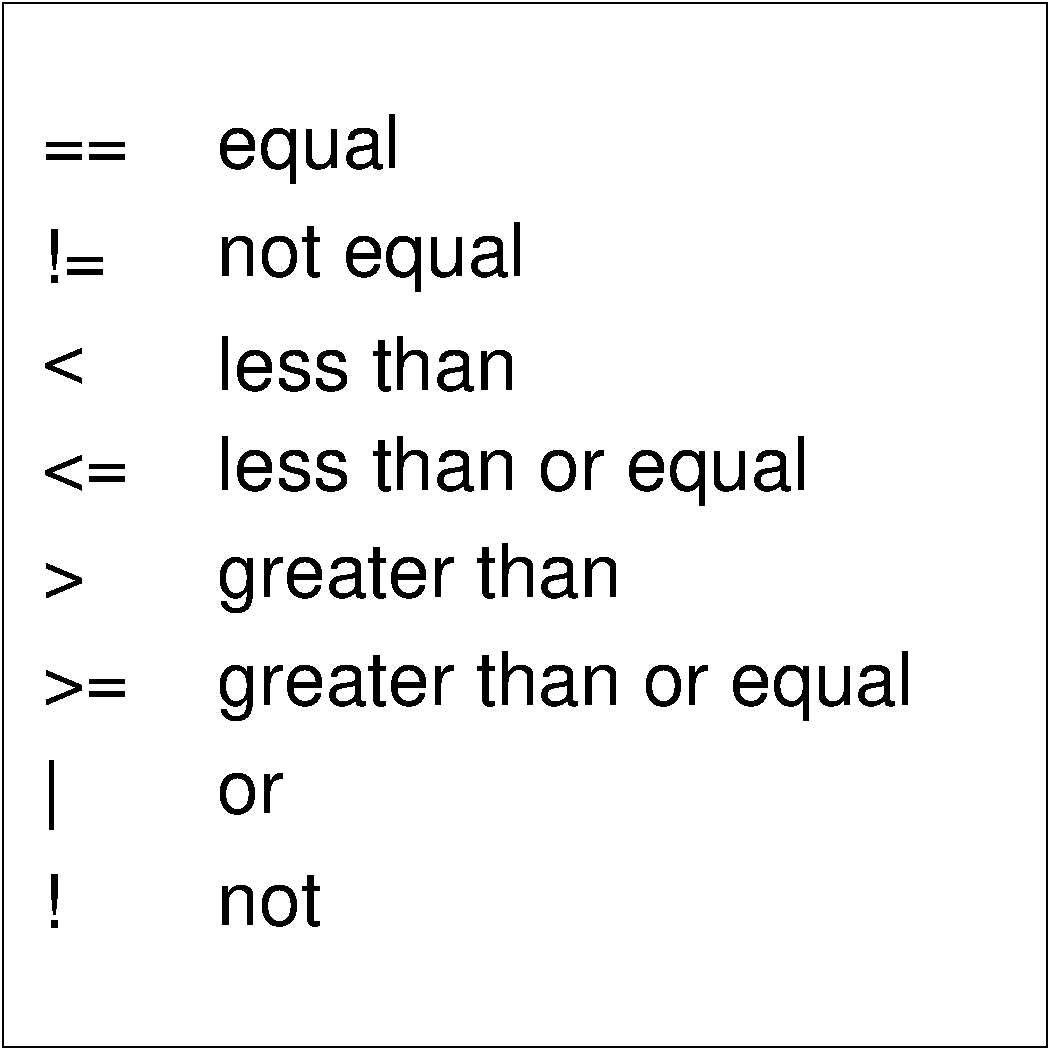
\includegraphics[width=\maxwidth]{figure/unnamed-chunk-76-1} 

\end{knitrout}
\caption{Comparison operators in R}
\label{fig:comparison}
\end{tiny}
\end{marginfigure}



\begin{marginfigure}
\begin{tiny}
\begin{knitrout}
\definecolor{shadecolor}{rgb}{0.969, 0.969, 0.969}\color{fgcolor}\begin{kframe}
\begin{alltt}
\hlcom{# Create blank plot with no margins}
\hlkwd{par}\hlstd{(}\hlkwc{mar} \hlstd{=} \hlkwd{rep}\hlstd{(}\hlnum{0}\hlstd{,} \hlnum{4}\hlstd{))}
\hlkwd{plot}\hlstd{(}\hlnum{1}\hlstd{,} \hlkwc{xlim} \hlstd{=} \hlkwd{c}\hlstd{(}\hlnum{0}\hlstd{,} \hlnum{1}\hlstd{),} \hlkwc{ylim} \hlstd{=} \hlkwd{c}\hlstd{(}\hlnum{0}\hlstd{,} \hlnum{13}\hlstd{),}
     \hlkwc{bty} \hlstd{=} \hlstr{"n"}\hlstd{,} \hlkwc{xlab} \hlstd{=} \hlstr{""}\hlstd{,} \hlkwc{ylab} \hlstd{=} \hlstr{""}\hlstd{,} \hlkwc{main} \hlstd{=} \hlstr{""}\hlstd{,}
     \hlkwc{type} \hlstd{=} \hlstr{"n"}\hlstd{,} \hlkwc{xaxt} \hlstd{=} \hlstr{"n"}\hlstd{,} \hlkwc{yaxt} \hlstd{=} \hlstr{"n"}\hlstd{)}

\hlcom{# Add Main title}
\hlkwd{text}\hlstd{(}\hlnum{.5}\hlstd{,} \hlnum{12.5}\hlstd{,} \hlstr{"log.vec <- data.vec > 0"}\hlstd{,} \hlkwc{cex} \hlstd{=} \hlnum{2}\hlstd{)}

\hlcom{# Data vector}
\hlkwd{text}\hlstd{(}\hlnum{.3}\hlstd{,} \hlnum{11.1}\hlstd{,} \hlstr{"data.vec"}\hlstd{,} \hlkwc{font} \hlstd{=} \hlnum{2}\hlstd{,} \hlkwc{cex} \hlstd{=} \hlnum{1.6}\hlstd{)}
\hlstd{data.vec} \hlkwb{<-} \hlkwd{c}\hlstd{(}\hlnum{2}\hlstd{,} \hlnum{7}\hlstd{,} \hlopt{-}\hlnum{1}\hlstd{,} \hlnum{5}\hlstd{,} \hlopt{-}\hlnum{9}\hlstd{,} \hlopt{-}\hlnum{2}\hlstd{,} \hlnum{3}\hlstd{,} \hlnum{0}\hlstd{,} \hlnum{2}\hlstd{,} \hlopt{-}\hlnum{2}\hlstd{)}
\hlkwd{text}\hlstd{(}\hlkwd{rep}\hlstd{(}\hlnum{.3}\hlstd{,} \hlnum{10}\hlstd{),} \hlnum{10}\hlopt{:}\hlnum{1}\hlstd{, data.vec,} \hlkwc{cex} \hlstd{=} \hlnum{1.6}\hlstd{)}
\hlkwd{rect}\hlstd{(}\hlnum{.25}\hlstd{,} \hlnum{.5}\hlstd{,} \hlnum{.35}\hlstd{,} \hlnum{10.5}\hlstd{)}
\hlkwd{segments}\hlstd{(}\hlkwd{rep}\hlstd{(}\hlnum{.25}\hlstd{,} \hlnum{9}\hlstd{),} \hlkwd{seq}\hlstd{(}\hlnum{1.5}\hlstd{,} \hlnum{9.5}\hlstd{,} \hlnum{1}\hlstd{),}
         \hlkwd{rep}\hlstd{(}\hlnum{.35}\hlstd{,} \hlnum{9}\hlstd{),} \hlkwd{seq}\hlstd{(}\hlnum{1.5}\hlstd{,} \hlnum{9.5}\hlstd{,} \hlnum{1}\hlstd{),} \hlkwc{lty} \hlstd{=} \hlnum{2}\hlstd{)}


\hlcom{# Comparisons}
\hlkwd{text}\hlstd{(}\hlnum{.5}\hlstd{,} \hlnum{11.1}\hlstd{,} \hlstr{"test"}\hlstd{,} \hlkwc{cex} \hlstd{=} \hlnum{1.6}\hlstd{,} \hlkwc{col} \hlstd{=} \hlkwd{gray}\hlstd{(}\hlnum{.5}\hlstd{))}
\hlkwd{text}\hlstd{(}\hlkwd{rep}\hlstd{(}\hlnum{.5}\hlstd{,} \hlnum{10}\hlstd{),} \hlnum{1}\hlopt{:}\hlnum{10}\hlstd{,} \hlstr{"> 0"}\hlstd{,} \hlkwc{col} \hlstd{=} \hlkwd{gray}\hlstd{(}\hlnum{.5}\hlstd{))}

\hlcom{# Logical vector}
\hlkwd{text}\hlstd{(}\hlnum{.7}\hlstd{,} \hlnum{11.1}\hlstd{,} \hlstr{"log.vec"}\hlstd{,} \hlkwc{font} \hlstd{=} \hlnum{2}\hlstd{,} \hlkwc{cex} \hlstd{=} \hlnum{1.6}\hlstd{)}
\hlstd{index.text} \hlkwb{<-} \hlkwd{rep}\hlstd{(}\hlstr{"FALSE"}\hlstd{,} \hlnum{10}\hlstd{)}
\hlstd{index.text[data.vec} \hlopt{>} \hlnum{0}\hlstd{]} \hlkwb{<-} \hlstr{"TRUE"}
\hlstd{col.vec} \hlkwb{<-} \hlkwd{rep}\hlstd{(}\hlstr{"red"}\hlstd{,} \hlnum{10}\hlstd{)}
\hlstd{col.vec[data.vec} \hlopt{>} \hlnum{0}\hlstd{]} \hlkwb{<-} \hlstr{"blue"}
\hlkwd{text}\hlstd{(}\hlkwd{rep}\hlstd{(}\hlnum{.7}\hlstd{,} \hlnum{10}\hlstd{),} \hlnum{10}\hlopt{:}\hlnum{1}\hlstd{,}
     \hlstd{index.text,}
     \hlkwc{col} \hlstd{= col.vec,} \hlkwc{cex} \hlstd{=} \hlnum{1.6}
     \hlstd{)}
\hlkwd{rect}\hlstd{(}\hlnum{.6}\hlstd{,} \hlnum{.7}\hlstd{,} \hlnum{.8}\hlstd{,} \hlnum{10.5}\hlstd{)}
\hlkwd{segments}\hlstd{(}\hlkwd{rep}\hlstd{(}\hlnum{.6}\hlstd{,} \hlnum{9}\hlstd{),} \hlkwd{seq}\hlstd{(}\hlnum{1.5}\hlstd{,} \hlnum{9.5}\hlstd{,} \hlnum{1}\hlstd{),}
         \hlkwd{rep}\hlstd{(}\hlnum{.8}\hlstd{,} \hlnum{9}\hlstd{),} \hlkwd{seq}\hlstd{(}\hlnum{1.5}\hlstd{,} \hlnum{9.5}\hlstd{,} \hlnum{1}\hlstd{),} \hlkwc{lty} \hlstd{=} \hlnum{2}\hlstd{)}
\end{alltt}
\end{kframe}
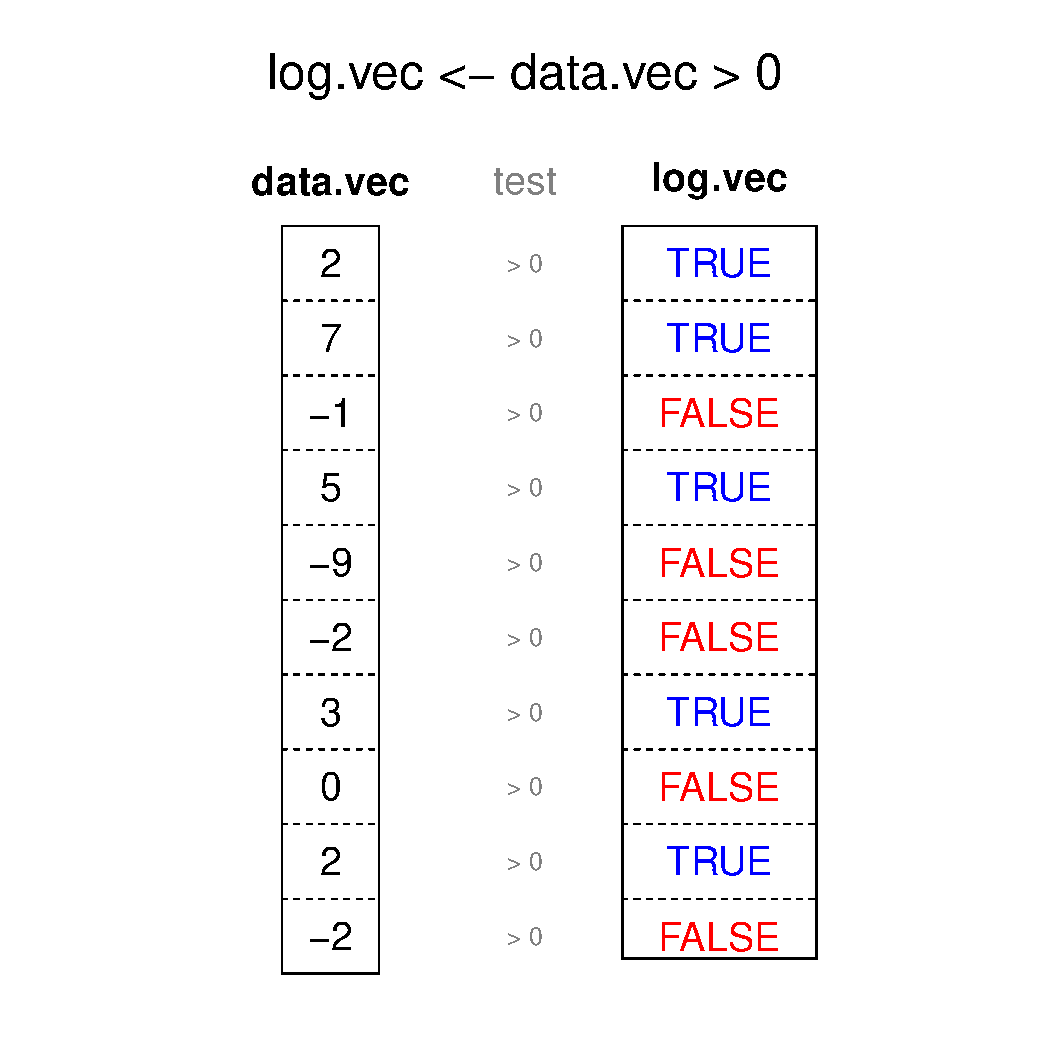
\includegraphics[width=\maxwidth]{figure/unnamed-chunk-77-1} 

\end{knitrout}
\end{tiny}
\label{fig:logvec1}
\caption{Creating a logical vector from a data vector with a comparison operator. In this case, the logical comparison is "> 0" and each element of the data vector is compared to 0.}
\end{marginfigure}

Another way to index data vectors is with logical vectors. A logical vector is a vector that only contains TRUE and FALSE values. If you index a vector with a logical vector (of the same length), you will only receive the values for which the index is TRUE.

You can create a logical vector by using the comparison operators in Figure~\ref{fig:comparison}.

Let's start by creating single scalar logical values so you can see how they work. If you apply a comparison operator to a scalar, R will return a single logical value of TRUE or FALSE. Let's see if 3 truly equals 3 and if 3 is really not greater than 5.


\begin{knitrout}
\definecolor{shadecolor}{rgb}{0.969, 0.969, 0.969}\color{fgcolor}\begin{kframe}
\begin{alltt}
\hlnum{3} \hlopt{==} \hlnum{3}
\end{alltt}
\begin{verbatim}
## [1] TRUE
\end{verbatim}
\begin{alltt}
\hlnum{3} \hlopt{>} \hlnum{5}
\end{alltt}
\begin{verbatim}
## [1] FALSE
\end{verbatim}
\end{kframe}
\end{knitrout}


The negation operator \texttt{!} meaning NOT. To use it, place the statement you are testing in parentheses, and place the \texttt{!} operator before it:


\begin{knitrout}
\definecolor{shadecolor}{rgb}{0.969, 0.969, 0.969}\color{fgcolor}\begin{kframe}
\begin{alltt}
\hlstd{pirate} \hlkwb{<-} \hlstr{"david"}
\hlstd{pirate} \hlopt{==} \hlstr{"jack"}
\end{alltt}
\begin{verbatim}
## [1] FALSE
\end{verbatim}
\begin{alltt}
\hlopt{!}\hlstd{(pirate} \hlopt{==} \hlstr{"jack"}\hlstd{)}
\end{alltt}
\begin{verbatim}
## [1] TRUE
\end{verbatim}
\begin{alltt}
\hlopt{!}\hlstd{(}\hlnum{2} \hlopt{==} \hlnum{4}\hlstd{)}
\end{alltt}
\begin{verbatim}
## [1] TRUE
\end{verbatim}
\end{kframe}
\end{knitrout}





In addition to using single comparison operators, you can combine multiple logical comparisons using the OR \texttt{|} and AND \texttt{\&} commands. The OR command will return TRUE if any of the values in the set is TRUE, while the AND command will only return TRUE if all of the values in the set are TRUE.


\begin{knitrout}
\definecolor{shadecolor}{rgb}{0.969, 0.969, 0.969}\color{fgcolor}\begin{kframe}
\begin{alltt}
\hlstd{(}\hlnum{1} \hlopt{<} \hlnum{3}\hlstd{)} \hlcom{# Is 1 less than 3?}
\end{alltt}
\begin{verbatim}
## [1] TRUE
\end{verbatim}
\begin{alltt}
\hlstd{(}\hlnum{4} \hlopt{<} \hlnum{2}\hlstd{)} \hlcom{# Is 4 less than 2?}
\end{alltt}
\begin{verbatim}
## [1] FALSE
\end{verbatim}
\begin{alltt}
\hlstd{(}\hlnum{1} \hlopt{<} \hlnum{3}\hlstd{)} \hlopt{&} \hlstd{(}\hlnum{4} \hlopt{<} \hlnum{2}\hlstd{)} \hlcom{# Is 1 less than 3 and is 4 less than 2?}
\end{alltt}
\begin{verbatim}
## [1] FALSE
\end{verbatim}
\begin{alltt}
\hlstd{(}\hlnum{1} \hlopt{<} \hlnum{3}\hlstd{)} \hlopt{|} \hlstd{(}\hlnum{4} \hlopt{<} \hlnum{2}\hlstd{)} \hlcom{# Is 1 less than 3 OR is 4 less than 2?}
\end{alltt}
\begin{verbatim}
## [1] TRUE
\end{verbatim}
\end{kframe}
\end{knitrout}


If you apply a comparison operator between a scalar and a vector, R will return a logical vector of length equal to the length of the vector. For example, let's compare a vector of integers from 1 to 10 to a scalar value of three and look at the output:


\begin{knitrout}
\definecolor{shadecolor}{rgb}{0.969, 0.969, 0.969}\color{fgcolor}\begin{kframe}
\begin{alltt}
\hlnum{1}\hlopt{:}\hlnum{10} \hlopt{==} \hlnum{3} \hlcom{# Are the values equal to 3?}
\end{alltt}
\begin{verbatim}
##  [1] FALSE FALSE  TRUE FALSE FALSE FALSE FALSE FALSE FALSE FALSE
\end{verbatim}
\end{kframe}
\end{knitrout}

Let's look at the outputs above: for each value of the object \texttt{vec}, R performs the comparison \texttt{== 3}. Because only the third element of the vector is equal to 3, R returns the value \texttt{FALSE} for all values except the third one.

You can also compare two vectors of equal length and obtain a single logical vector as a result. For example, let's say we have two data vectors (data.1 and data.2) and we want a logical vector telling us which values of the two data vectors are equal. We can do this by just executing \texttt{data.1 == data.2}

\begin{footnotesize}
\begin{knitrout}
\definecolor{shadecolor}{rgb}{0.969, 0.969, 0.969}\color{fgcolor}\begin{kframe}
\begin{alltt}
\hlstd{data.1} \hlkwb{<-} \hlkwd{c}\hlstd{(}\hlnum{1}\hlstd{,} \hlnum{4}\hlstd{,} \hlnum{2}\hlstd{,} \hlnum{3}\hlstd{,} \hlnum{3}\hlstd{)}
\hlstd{data.2} \hlkwb{<-} \hlkwd{c}\hlstd{(}\hlnum{1}\hlstd{,} \hlnum{2}\hlstd{,} \hlnum{4}\hlstd{,} \hlnum{3}\hlstd{,} \hlnum{3}\hlstd{)}
\hlstd{data.1} \hlopt{==} \hlstd{data.2}
\end{alltt}
\begin{verbatim}
## [1]  TRUE FALSE FALSE  TRUE  TRUE
\end{verbatim}
\end{kframe}
\end{knitrout}
\end{footnotesize}

\newfun{x \%in\% y}\index{\%in\%}

One very important function for creating logical indices is \texttt{\%in\%}. This function looks a bit different from other functions because it doesn't follow the typical format of function(x, y). Instead, you place the function \%in\% between its arguments. When you execute x \%in\% y, R will evaluate, for each element in the vector x, if it is in the vector y. For example. Let's create several vectors x and y and use the \%in\% function to text whether or not the elements of x are in y:


\begin{knitrout}
\definecolor{shadecolor}{rgb}{0.969, 0.969, 0.969}\color{fgcolor}\begin{kframe}
\begin{alltt}
\hlnum{1} \hlopt \hlkwd{c}\hlstd{(}\hlnum{1}\hlstd{,} \hlnum{2}\hlstd{,} \hlnum{3}\hlstd{,} \hlnum{4}\hlstd{,} \hlnum{5}\hlstd{)}
\end{alltt}
\begin{verbatim}
## [1] TRUE
\end{verbatim}
\end{kframe}
\end{knitrout}


In this example, R returns a single value of TRUE because it found the value of 1 in the second vector. However, you can also apply the \%in\% function to a vector x that is longer than 1. When you do this, the \%in\% function will return a vector equal to the length of x. Now, let's try an example where we test whether each of several values are in a second set:


\begin{knitrout}
\definecolor{shadecolor}{rgb}{0.969, 0.969, 0.969}\color{fgcolor}\begin{kframe}
\begin{alltt}
\hlkwd{c}\hlstd{(}\hlnum{1}\hlstd{,} \hlnum{2}\hlstd{,} \hlnum{3}\hlstd{,} \hlnum{77}\hlstd{,} \hlnum{88}\hlstd{,} \hlnum{99}\hlstd{)} \hlopt \hlkwd{c}\hlstd{(}\hlnum{1}\hlstd{,} \hlnum{2}\hlstd{,} \hlnum{3}\hlstd{,} \hlnum{4}\hlstd{,} \hlnum{5}\hlstd{)}
\end{alltt}
\begin{verbatim}
## [1]  TRUE  TRUE  TRUE FALSE FALSE FALSE
\end{verbatim}
\end{kframe}
\end{knitrout}


In this example R checked, for each of the values in the first vector if it was in the second vector (\texttt{c(1, 2, 3, 4, 5)}). Because only the first three values (1, 2 and 3) were in the second vector, R returns a vector with 3 TRUE values and 3 FALSE values.

The \%in\% function is very handy for seeing which values in a vector are valid according to a criteria you specify. For example, imagine you conducted a survey where you asked 10 different pirates how many siblings they had and received the following responses:

\begin{knitrout}
\definecolor{shadecolor}{rgb}{0.969, 0.969, 0.969}\color{fgcolor}\begin{kframe}
\begin{alltt}
\hlstd{siblings} \hlkwb{<-} \hlkwd{c}\hlstd{(}\hlnum{3}\hlstd{,} \hlnum{2}\hlstd{,} \hlnum{0}\hlstd{,} \hlopt{-}\hlnum{5}\hlstd{,} \hlnum{0}\hlstd{,} \hlopt{-}\hlnum{20}\hlstd{,} \hlnum{2}\hlstd{,} \hlnum{3}\hlstd{,} \hlnum{1}\hlstd{,} \hlopt{-}\hlnum{200}\hlstd{)}
\end{alltt}
\end{kframe}
\end{knitrout}

Of course, the only valid answers to this question should be 0, 1, 2, ... up to a maximum of say 20; but some of these values appear to be invalid (that is, negative). Let's use the \%in\% function to see which values in the survey are valid. We'll create a vector called \texttt{valid.responses} that represents all possible valid answers to the question (we'll limit the number of siblings to 20). We'll then use \%in\% to create a logical vector indicating which responses were valid.


\begin{knitrout}
\definecolor{shadecolor}{rgb}{0.969, 0.969, 0.969}\color{fgcolor}\begin{kframe}
\begin{alltt}
\hlstd{siblings} \hlkwb{<-} \hlkwd{c}\hlstd{(}\hlnum{3}\hlstd{,} \hlnum{2}\hlstd{,} \hlnum{0}\hlstd{,} \hlopt{-}\hlnum{5}\hlstd{,} \hlnum{0}\hlstd{,} \hlopt{-}\hlnum{20}\hlstd{,} \hlnum{2}\hlstd{,} \hlnum{3}\hlstd{,} \hlnum{1}\hlstd{,} \hlopt{-}\hlnum{200}\hlstd{)}
\hlstd{valid.responses} \hlkwb{<-} \hlkwd{seq}\hlstd{(}\hlnum{0}\hlstd{,} \hlnum{20}\hlstd{,} \hlnum{1}\hlstd{)}
\hlstd{siblings} \hlopt \hlstd{valid.responses}
\end{alltt}
\begin{verbatim}
##  [1]  TRUE  TRUE  TRUE FALSE  TRUE FALSE  TRUE  TRUE  TRUE FALSE
\end{verbatim}
\end{kframe}
\end{knitrout}


Because the fourth, sixth, and tenth values were not valid (they were negative), the final logical vector gives us FALSE values at those index values, and TRUE values for all others.

\section{Indexing data with logical vectors}

\begin{marginfigure}
\begin{tiny}
\begin{knitrout}
\definecolor{shadecolor}{rgb}{0.969, 0.969, 0.969}\color{fgcolor}\begin{kframe}
\begin{alltt}
\hlcom{# Create blank plot with no margins}
\hlkwd{par}\hlstd{(}\hlkwc{mar} \hlstd{=} \hlkwd{rep}\hlstd{(}\hlnum{0}\hlstd{,} \hlnum{4}\hlstd{))}
\hlkwd{plot}\hlstd{(}\hlnum{1}\hlstd{,} \hlkwc{xlim} \hlstd{=} \hlkwd{c}\hlstd{(}\hlnum{0}\hlstd{,} \hlnum{1}\hlstd{),} \hlkwc{ylim} \hlstd{=} \hlkwd{c}\hlstd{(}\hlnum{0}\hlstd{,} \hlnum{13}\hlstd{),}
     \hlkwc{bty} \hlstd{=} \hlstr{"n"}\hlstd{,} \hlkwc{xlab} \hlstd{=} \hlstr{""}\hlstd{,} \hlkwc{ylab} \hlstd{=} \hlstr{""}\hlstd{,} \hlkwc{main} \hlstd{=} \hlstr{""}\hlstd{,}
     \hlkwc{type} \hlstd{=} \hlstr{"n"}\hlstd{,} \hlkwc{xaxt} \hlstd{=} \hlstr{"n"}\hlstd{,} \hlkwc{yaxt} \hlstd{=} \hlstr{"n"}\hlstd{)}

\hlcom{# Add Main title}
\hlkwd{text}\hlstd{(}\hlnum{.5}\hlstd{,} \hlnum{12.5}\hlstd{,} \hlstr{"output.vec <- data.vec[log.vec]"}\hlstd{,} \hlkwc{cex} \hlstd{=} \hlnum{2}\hlstd{)}

\hlcom{# Data vector}
\hlkwd{text}\hlstd{(}\hlnum{.2}\hlstd{,} \hlnum{11.1}\hlstd{,} \hlstr{"data.vec"}\hlstd{,} \hlkwc{font} \hlstd{=} \hlnum{2}\hlstd{,} \hlkwc{cex} \hlstd{=} \hlnum{1.6}\hlstd{)}
\hlstd{data.vec} \hlkwb{<-} \hlkwd{c}\hlstd{(}\hlnum{2}\hlstd{,} \hlnum{7}\hlstd{,} \hlopt{-}\hlnum{1}\hlstd{,} \hlnum{5}\hlstd{,} \hlopt{-}\hlnum{9}\hlstd{,} \hlopt{-}\hlnum{2}\hlstd{,} \hlnum{3}\hlstd{,} \hlnum{0}\hlstd{,} \hlnum{2}\hlstd{,} \hlopt{-}\hlnum{2}\hlstd{)}
\hlkwd{text}\hlstd{(}\hlkwd{rep}\hlstd{(}\hlnum{.2}\hlstd{,} \hlnum{10}\hlstd{),} \hlnum{10}\hlopt{:}\hlnum{1}\hlstd{, data.vec,} \hlkwc{cex} \hlstd{=} \hlnum{1.6}\hlstd{)}
\hlkwd{rect}\hlstd{(}\hlnum{.15}\hlstd{,} \hlnum{.5}\hlstd{,} \hlnum{.25}\hlstd{,} \hlnum{10.5}\hlstd{)}
\hlkwd{segments}\hlstd{(}\hlkwd{rep}\hlstd{(}\hlnum{.15}\hlstd{,} \hlnum{9}\hlstd{),} \hlkwd{seq}\hlstd{(}\hlnum{1.5}\hlstd{,} \hlnum{9.5}\hlstd{,} \hlnum{1}\hlstd{),}
         \hlkwd{rep}\hlstd{(}\hlnum{.25}\hlstd{,} \hlnum{9}\hlstd{),} \hlkwd{seq}\hlstd{(}\hlnum{1.5}\hlstd{,} \hlnum{9.5}\hlstd{,} \hlnum{1}\hlstd{),} \hlkwc{lty} \hlstd{=} \hlnum{2}\hlstd{)}
\hlkwd{text}\hlstd{(}\hlkwd{rep}\hlstd{(}\hlnum{.12}\hlstd{,} \hlnum{10}\hlstd{),} \hlnum{10}\hlopt{:}\hlnum{1}\hlstd{,} \hlnum{1}\hlopt{:}\hlnum{10}\hlstd{,} \hlkwc{cex} \hlstd{=} \hlnum{.8}\hlstd{)}

\hlcom{# Comparisons}
\hlkwd{text}\hlstd{(}\hlkwd{rep}\hlstd{(}\hlnum{.32}\hlstd{,} \hlnum{10}\hlstd{),} \hlnum{1}\hlopt{:}\hlnum{10}\hlstd{,} \hlstr{"> 0"}\hlstd{,} \hlkwc{col} \hlstd{=} \hlkwd{gray}\hlstd{(}\hlnum{.5}\hlstd{))}

\hlcom{# Logical vector}
\hlkwd{text}\hlstd{(}\hlnum{.5}\hlstd{,} \hlnum{11.1}\hlstd{,} \hlstr{"log.vec"}\hlstd{,} \hlkwc{font} \hlstd{=} \hlnum{2}\hlstd{,} \hlkwc{cex} \hlstd{=} \hlnum{1.6}\hlstd{)}
\hlstd{index.text} \hlkwb{<-} \hlkwd{rep}\hlstd{(}\hlstr{"FALSE"}\hlstd{,} \hlnum{10}\hlstd{)}
\hlstd{index.text[data.vec} \hlopt{>} \hlnum{0}\hlstd{]} \hlkwb{<-} \hlstr{"TRUE"}
\hlstd{col.vec} \hlkwb{<-} \hlkwd{rep}\hlstd{(}\hlstr{"red"}\hlstd{,} \hlnum{10}\hlstd{)}
\hlstd{col.vec[data.vec} \hlopt{>} \hlnum{0}\hlstd{]} \hlkwb{<-} \hlstr{"blue"}
\hlkwd{text}\hlstd{(}\hlkwd{rep}\hlstd{(}\hlnum{.5}\hlstd{,} \hlnum{10}\hlstd{),} \hlnum{10}\hlopt{:}\hlnum{1}\hlstd{,}
     \hlstd{index.text,}
     \hlkwc{col} \hlstd{= col.vec,} \hlkwc{cex} \hlstd{=} \hlnum{1.6}
     \hlstd{)}
\hlkwd{rect}\hlstd{(}\hlnum{.4}\hlstd{,} \hlnum{.5}\hlstd{,} \hlnum{.6}\hlstd{,} \hlnum{10.5}\hlstd{)}
\hlkwd{segments}\hlstd{(}\hlkwd{rep}\hlstd{(}\hlnum{.4}\hlstd{,} \hlnum{9}\hlstd{),} \hlkwd{seq}\hlstd{(}\hlnum{1.5}\hlstd{,} \hlnum{9.5}\hlstd{,} \hlnum{1}\hlstd{),}
         \hlkwd{rep}\hlstd{(}\hlnum{.6}\hlstd{,} \hlnum{9}\hlstd{),} \hlkwd{seq}\hlstd{(}\hlnum{1.5}\hlstd{,} \hlnum{9.5}\hlstd{,} \hlnum{1}\hlstd{),} \hlkwc{lty} \hlstd{=} \hlnum{2}\hlstd{)}

\hlcom{# Output vector}
\hlkwd{text}\hlstd{(}\hlnum{.8}\hlstd{,} \hlnum{11.1}\hlstd{,} \hlstr{"output.vec"}\hlstd{,} \hlkwc{font} \hlstd{=} \hlnum{2}\hlstd{,} \hlkwc{cex} \hlstd{=} \hlnum{1.6}\hlstd{)}
\hlstd{output.text} \hlkwb{<-} \hlstd{data.vec[data.vec} \hlopt{>} \hlnum{0}\hlstd{]}
\hlkwd{text}\hlstd{(}\hlkwd{rep}\hlstd{(}\hlnum{.8}\hlstd{,} \hlnum{5}\hlstd{),} \hlnum{7}\hlopt{:}\hlnum{3}\hlstd{, output.text,} \hlkwc{cex} \hlstd{=} \hlnum{1.6}\hlstd{)}
\hlkwd{rect}\hlstd{(}\hlnum{.75}\hlstd{,} \hlnum{2.5}\hlstd{,} \hlnum{.85}\hlstd{,} \hlnum{7.5}\hlstd{)}
\hlkwd{segments}\hlstd{(}\hlkwd{rep}\hlstd{(}\hlnum{.75}\hlstd{,} \hlnum{9}\hlstd{),} \hlkwd{seq}\hlstd{(}\hlnum{3.5}\hlstd{,} \hlnum{6.5}\hlstd{,} \hlnum{1}\hlstd{),}
         \hlkwd{rep}\hlstd{(}\hlnum{.85}\hlstd{,} \hlnum{9}\hlstd{),} \hlkwd{seq}\hlstd{(}\hlnum{3.5}\hlstd{,} \hlnum{6.5}\hlstd{,} \hlnum{1}\hlstd{),} \hlkwc{lty} \hlstd{=} \hlnum{2}\hlstd{)}
\hlkwd{text}\hlstd{(}\hlkwd{rep}\hlstd{(}\hlnum{.88}\hlstd{,} \hlnum{5}\hlstd{),} \hlnum{7}\hlopt{:}\hlnum{3}\hlstd{,} \hlkwd{which}\hlstd{(data.vec} \hlopt{>} \hlnum{0}\hlstd{),} \hlkwc{cex} \hlstd{=} \hlnum{.8}\hlstd{)}

\hlcom{# Arrows connecting log.vec to output.vec}
\hlkwd{arrows}\hlstd{(}\hlkwd{rep}\hlstd{(}\hlnum{.6}\hlstd{,} \hlnum{5}\hlstd{),}
       \hlnum{11} \hlopt{-} \hlkwd{which}\hlstd{(data.vec} \hlopt{>} \hlnum{0}\hlstd{),}
       \hlkwd{rep}\hlstd{(}\hlnum{.73}\hlstd{,} \hlnum{5}\hlstd{),}
       \hlnum{7}\hlopt{:}\hlnum{3}\hlstd{,} \hlkwc{lwd} \hlstd{=} \hlnum{.5}\hlstd{,} \hlkwc{length} \hlstd{=} \hlnum{.15}
       \hlstd{)}
\end{alltt}
\end{kframe}
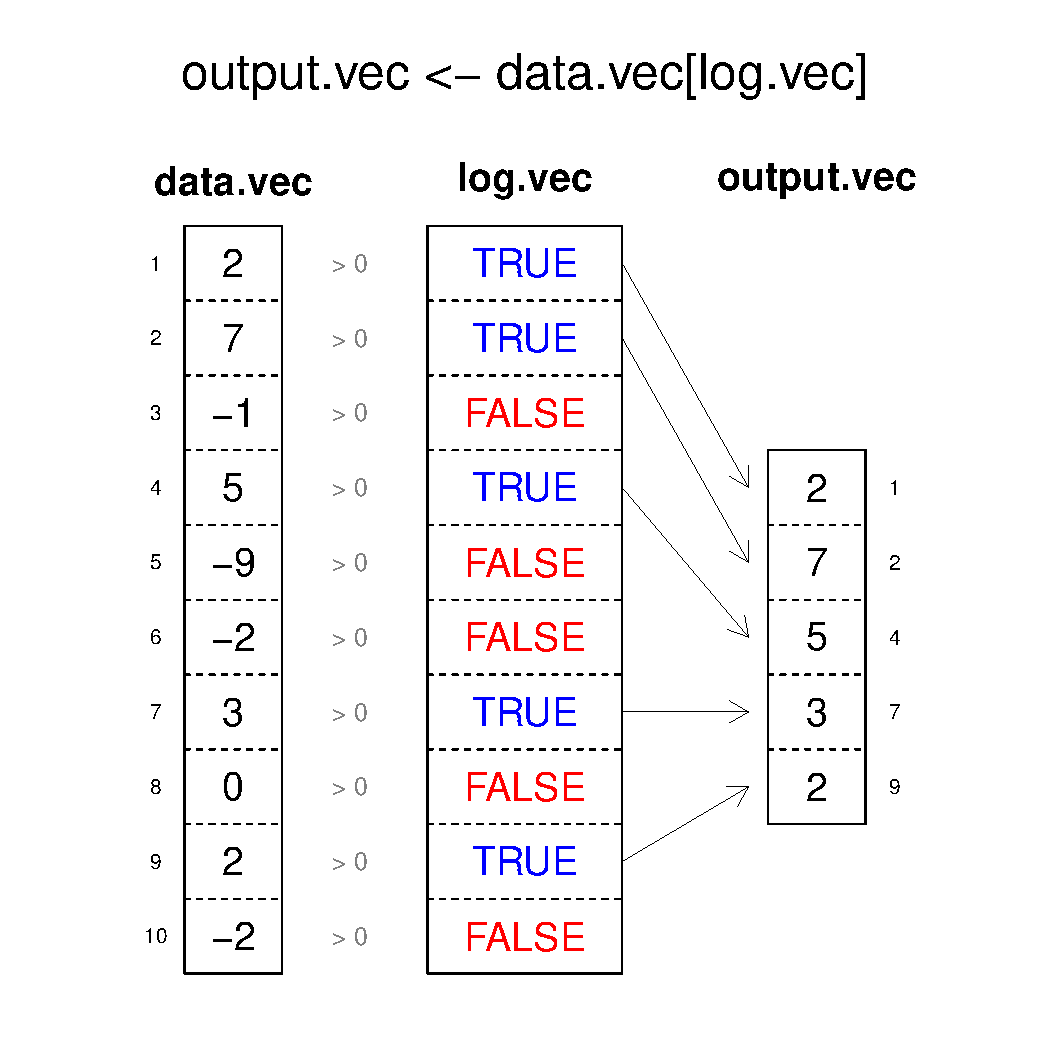
\includegraphics[width=\maxwidth]{figure/unnamed-chunk-87-1} 

\end{knitrout}
\end{tiny}
\label{fig:logvec2}
\caption{A visual representation of how indexing with logical vectors works in R. When you apply a logical vector (a vector containing only TRUE and FALSE values) to a data vector, R will return the the values in the data vector where the logical vector is TRUE.}
\end{marginfigure}

Once we have a logical vector, we can use that vector as an indexing vector. That is, you can use it to select values of a vector that satisfy some criteria you specify. To do this, you create a logical vector containing TRUE and FALSE values. If you then index a data vector (with the same length as the logical vector), R will return the values of the data vector for all TRUE values of the logical vector. See Figure~\ref{fig:logvec2} to see visually how this works.


For example, let's say that we have the following set of data


\begin{knitrout}
\definecolor{shadecolor}{rgb}{0.969, 0.969, 0.969}\color{fgcolor}\begin{kframe}
\begin{alltt}
\hlstd{tattoos} \hlkwb{<-} \hlkwd{c}\hlstd{(}\hlnum{4}\hlstd{,} \hlnum{50}\hlstd{,} \hlnum{2}\hlstd{,} \hlnum{39}\hlstd{,} \hlnum{4}\hlstd{,} \hlnum{20}\hlstd{,} \hlnum{4}\hlstd{,} \hlnum{8}\hlstd{,} \hlnum{10}\hlstd{,} \hlnum{100}\hlstd{)}
\end{alltt}
\end{kframe}
\end{knitrout}


Now, let's say that we want to access just the data points that are less than 10. We'll start by first creating a logical indexing vector that tells us whether each value is less than 1. Then, we'll index the original data vector using this logical vector:


\begin{knitrout}
\definecolor{shadecolor}{rgb}{0.969, 0.969, 0.969}\color{fgcolor}\begin{kframe}
\begin{alltt}
\hlstd{log.vec} \hlkwb{<-} \hlstd{tattoos} \hlopt{<} \hlnum{10} \hlcom{# Step 1: Create logical vector}
\hlstd{tattoos[log.vec]} \hlcom{# Step 2: Index the original data by the logical vector}
\end{alltt}
\begin{verbatim}
## [1] 4 2 4 4 8
\end{verbatim}
\end{kframe}
\end{knitrout}



Logical vectors aren't just good for indexing, you can also use them to figure out which values in a vector satisfy some criteria. To do this, use the function \textt{which()}

\newfun{which(log.vec)}%\marginnote{\texttt{\textbf{which(logical.vector)}}: Tells you the index value of all \texttt{TRUE} values in the logical vector. \\ For example, the command \texttt{which(c(T, T, F))} will return the vector \texttt{[1, 2]}, telling you that the first and second values are true.}

If you apply the function \texttt{which()} to a logical vector, R will tell you which values of the index are TRUE. For example, let's create a logical vector and then see which index values are TRUE

\begin{knitrout}
\definecolor{shadecolor}{rgb}{0.969, 0.969, 0.969}\color{fgcolor}\begin{kframe}
\begin{alltt}
\hlstd{log.vec} \hlkwb{<-} \hlkwd{c}\hlstd{(}\hlnum{TRUE}\hlstd{,} \hlnum{TRUE}\hlstd{,} \hlnum{FALSE}\hlstd{,} \hlnum{TRUE}\hlstd{,} \hlnum{FALSE}\hlstd{)}
\hlkwd{which}\hlstd{(log.vec)}
\end{alltt}
\begin{verbatim}
## [1] 1 2 4
\end{verbatim}
\end{kframe}
\end{knitrout}

By using the \texttt{which()} function, we know that the first, second, and fourth elements of the logical vector are TRUE.

Let's take the example of comparing the treasure chest finding ability of 10 pirates. In each of two years - 2014 and 2015 - I measured how many chests 10 pirates found over the entire year. I recorded these values in two vectors, where the first value of each vector corresponds to the first pirate, and the last value corresponds to the last pirate:


\begin{knitrout}
\definecolor{shadecolor}{rgb}{0.969, 0.969, 0.969}\color{fgcolor}\begin{kframe}
\begin{alltt}
\hlstd{pirate.names} \hlkwb{<-} \hlkwd{c}\hlstd{(}\hlstr{"Andrew"}\hlstd{,} \hlstr{"Heidi"}\hlstd{,} \hlstr{"Madisen"}\hlstd{,} \hlstr{"Becki"}\hlstd{,} \hlstr{"Jack Dyanamite"}\hlstd{)}
\hlstd{chests.2014} \hlkwb{<-} \hlkwd{c}\hlstd{(}\hlnum{0}\hlstd{,} \hlnum{10}\hlstd{,} \hlnum{1}\hlstd{,} \hlnum{2}\hlstd{,} \hlnum{5}\hlstd{)}
\hlstd{chests.2015} \hlkwb{<-} \hlkwd{c}\hlstd{(}\hlnum{0}\hlstd{,} \hlnum{6}\hlstd{,} \hlnum{3}\hlstd{,} \hlnum{0}\hlstd{,} \hlnum{20}\hlstd{)}
\end{alltt}
\end{kframe}
\end{knitrout}


Ok, so let's see which pirates improved their chest finding ability. I'll start by finding the index values where the number of chests found increased between the two years


\begin{knitrout}
\definecolor{shadecolor}{rgb}{0.969, 0.969, 0.969}\color{fgcolor}\begin{kframe}
\begin{alltt}
\hlstd{improve.log} \hlkwb{<-} \hlstd{chests.2015} \hlopt{>} \hlstd{chests.2014} \hlcom{# create logical vector}
\hlstd{improve.log} \hlcom{# print values}
\end{alltt}
\begin{verbatim}
## [1] FALSE FALSE  TRUE FALSE  TRUE
\end{verbatim}
\end{kframe}
\end{knitrout}


If I want to know the index values of the pirates who improved, I can use the \texttt{which()} function. The which function will tell me the index of each TRUE value in a logical vector:


\begin{knitrout}
\definecolor{shadecolor}{rgb}{0.969, 0.969, 0.969}\color{fgcolor}\begin{kframe}
\begin{alltt}
\hlkwd{which}\hlstd{(improve.log)}
\end{alltt}
\begin{verbatim}
## [1] 3 5
\end{verbatim}
\end{kframe}
\end{knitrout}


This vector tells us that the 3rd and 5th pirates found more chests in 2015 than 2014. Now I can use this index value to figure out the names of those pirates:


\begin{knitrout}
\definecolor{shadecolor}{rgb}{0.969, 0.969, 0.969}\color{fgcolor}\begin{kframe}
\begin{alltt}
\hlstd{pirate.names[}\hlkwd{which}\hlstd{(improve.log)]}
\end{alltt}
\begin{verbatim}
## [1] "Madisen"        "Jack Dyanamite"
\end{verbatim}
\end{kframe}
\end{knitrout}



Because you can index vectors with logical vectors, I could get the same results by just indexing \texttt{pirate.names} with \texttt{improve.log}.


\begin{knitrout}
\definecolor{shadecolor}{rgb}{0.969, 0.969, 0.969}\color{fgcolor}\begin{kframe}
\begin{alltt}
\hlstd{pirate.names[improve.log]}
\end{alltt}
\begin{verbatim}
## [1] "Madisen"        "Jack Dyanamite"
\end{verbatim}
\end{kframe}
\end{knitrout}

For this example, the \texttt{which()} command was unnecessary, but it's important to understand the logic of both methods.

\section{Additional helpful vector functions}

Here are some other functions you might find useful when dealing with vectors:


\vspace{5mm} %5mm vertical space
\noindent
\setlength{\fboxrule}{1.5pt}
\fbox{
\parbox{\textwidth}{

\newfun{Other Helpful Vector Functions}

\hline

\begin{description}

\item[\tt{length(x)}] \hfill \\
    The length of a vector

\item[\tt{sort(x)}] \hfill \\
    Sort a vector x. Add the argument \texttt{decreasing = T} to sort in decreasing order.

\item[\tt{rev(x)}] \hfill \\
    Reverse the order of a vector x

\item[\tt{rank(x)}] \hfill \\
    Returns the sample ranks of the values in a vector. Ties (i.e.; equal values) and missing values can be handled in several ways using the \texttt{ties.method} argument.

\end{description}

}
}
\vspace{5mm} %5mm vertical space

Once you have a vector of data, you may want to sort it in order to see, for example, the largest and smallest values. You can do this using the \texttt{sort()} function. Let's look back on my summer joke data and sort the results:


\begin{knitrout}
\definecolor{shadecolor}{rgb}{0.969, 0.969, 0.969}\color{fgcolor}\begin{kframe}
\begin{alltt}
\hlstd{tattoos} \hlkwb{<-} \hlkwd{c}\hlstd{(}\hlnum{4}\hlstd{,} \hlnum{50}\hlstd{,} \hlnum{2}\hlstd{,} \hlnum{39}\hlstd{,} \hlnum{4}\hlstd{,} \hlnum{20}\hlstd{,} \hlnum{4}\hlstd{,} \hlnum{8}\hlstd{,} \hlnum{10}\hlstd{,} \hlnum{100}\hlstd{)}
\hlkwd{sort}\hlstd{(tattoos,} \hlkwc{decreasing} \hlstd{= T)} \hlcom{# Sort decreasing}
\end{alltt}
\begin{verbatim}
##  [1] 100  50  39  20  10   8   4   4   4   2
\end{verbatim}
\begin{alltt}
\hlkwd{sort}\hlstd{(tattoos,} \hlkwc{decreasing} \hlstd{= F)} \hlcom{# Sort increasing}
\end{alltt}
\begin{verbatim}
##  [1]   2   4   4   4   8  10  20  39  50 100
\end{verbatim}
\end{kframe}
\end{knitrout}


You'll notice that the sort function has an argument \texttt{decreasing} which you can set to TRUE or FALSE.


\section{Set Functions}

R contains many functions that allow you to compare two sets (vectors) of data. See margin Figure~\ref{fig:setfunctions} for a visual depiction. Here are the most common ones:



\vspace{5mm} %5mm vertical space
\noindent
\setlength{\fboxrule}{1.5pt}
\fbox{
\parbox{\textwidth}{

\newfun{Set Functions}

\hline

\begin{description}

\item[\tt{union(x, y)}] \hfill \\
Tells you all unique values included in \textit{either} the vector x or y.
\item[\tt{intersect(x, y)}] \hfill \\
   Tells you all values common in \textit{both} the vectors x and y.
\item[\tt{setdiff(x)}] \hfill \\
    Tells you which values are in the vector x but \textit{not} in the vector y. Keep in mind that \texttt{setdiff(x, y)} is \textit{not} the same as \texttt{setdiff{y, x}}!
\item[\tt{setequal(x)}] \hfill \\
Returns TRUE of the two vectors x and y are identical (ignoring order) and FALSE if they are not identical.

\end{description}

}
}
\vspace{5mm} %5mm vertical space



\begin{marginfigure}
\begin{tiny}
\begin{knitrout}
\definecolor{shadecolor}{rgb}{0.969, 0.969, 0.969}\color{fgcolor}\begin{kframe}
\begin{alltt}
\hlkwd{require}\hlstd{(}\hlstr{"plotrix"}\hlstd{)}
\end{alltt}


{\ttfamily\noindent\itshape\color{messagecolor}{\#\# Loading required package: plotrix}}

{\ttfamily\noindent\color{warningcolor}{\#\# Warning: package 'plotrix' was built under R version 3.2.3}}\begin{alltt}
\hlkwd{require}\hlstd{(}\hlstr{"RColorBrewer"}\hlstd{)}

\hlcom{# Transparent() is a function that makes transparent colors}
\hlstd{Transparent} \hlkwb{<-} \hlkwa{function}\hlstd{(}\hlkwc{orig.col} \hlstd{=} \hlstr{"red"}\hlstd{,}
                        \hlkwc{trans.val} \hlstd{=} \hlnum{1}\hlstd{,}
                        \hlkwc{maxColorValue} \hlstd{=} \hlnum{255}\hlstd{) \{}

  \hlstd{orig.col} \hlkwb{<-} \hlkwd{col2rgb}\hlstd{(orig.col)}

  \hlstd{final.col} \hlkwb{<-} \hlkwd{rgb}\hlstd{(orig.col[}\hlnum{1}\hlstd{],}
                   \hlstd{orig.col[}\hlnum{2}\hlstd{],}
                   \hlstd{orig.col[}\hlnum{3}\hlstd{],}
                   \hlkwc{alpha} \hlstd{= trans.val} \hlopt{*} \hlnum{255}\hlstd{,}
                   \hlkwc{maxColorValue} \hlstd{= maxColorValue)}

  \hlkwd{return}\hlstd{(final.col)}
\hlstd{\}}


\hlstd{color.vec} \hlkwb{<-} \hlkwd{brewer.pal}\hlstd{(}\hlnum{12}\hlstd{,} \hlstr{"Set3"}\hlstd{)}
\hlkwd{par}\hlstd{(}\hlkwc{mar} \hlstd{=} \hlkwd{rep}\hlstd{(}\hlnum{0}\hlstd{,} \hlnum{4}\hlstd{))}
\hlkwd{plot}\hlstd{(}\hlnum{1}\hlstd{,} \hlkwc{xlim} \hlstd{=} \hlkwd{c}\hlstd{(}\hlnum{0}\hlstd{,} \hlnum{1}\hlstd{),} \hlkwc{ylim} \hlstd{=} \hlkwd{c}\hlstd{(}\hlnum{0}\hlstd{,} \hlnum{1}\hlstd{),}
     \hlkwc{bty} \hlstd{=} \hlstr{"n"}\hlstd{,} \hlkwc{xlab} \hlstd{=} \hlstr{""}\hlstd{,} \hlkwc{ylab} \hlstd{=} \hlstr{""}\hlstd{,} \hlkwc{main} \hlstd{=} \hlstr{""}\hlstd{,}
     \hlkwc{type} \hlstd{=} \hlstr{"n"}\hlstd{,} \hlkwc{xaxt} \hlstd{=} \hlstr{"n"}\hlstd{,} \hlkwc{yaxt} \hlstd{=} \hlstr{"n"}\hlstd{)}

\hlkwd{draw.circle}\hlstd{(}\hlkwc{x} \hlstd{=} \hlnum{.35}\hlstd{,} \hlkwc{y} \hlstd{=} \hlnum{.5}\hlstd{,}
            \hlkwc{radius} \hlstd{=} \hlnum{.35}\hlstd{,}
            \hlkwc{col} \hlstd{=} \hlkwd{Transparent}\hlstd{(color.vec[}\hlnum{4}\hlstd{],} \hlnum{.3}\hlstd{),} \hlkwc{lwd} \hlstd{=} \hlnum{2}\hlstd{)}

\hlkwd{draw.circle}\hlstd{(}\hlkwc{x} \hlstd{=} \hlnum{.65}\hlstd{,} \hlkwc{y} \hlstd{=} \hlnum{.5}\hlstd{,}
            \hlkwc{radius} \hlstd{=} \hlnum{.35}\hlstd{,} \hlkwc{col} \hlstd{=} \hlkwd{Transparent}\hlstd{(color.vec[}\hlnum{5}\hlstd{],} \hlnum{.3}\hlstd{),}
            \hlkwc{lty} \hlstd{=} \hlnum{2}\hlstd{,} \hlkwc{lwd} \hlstd{=} \hlnum{2}\hlstd{)}

\hlkwd{text}\hlstd{(}\hlnum{.35}\hlstd{,} \hlnum{.1}\hlstd{,} \hlstr{"Set X"}\hlstd{,} \hlkwc{cex} \hlstd{=} \hlnum{1.5}\hlstd{)}
\hlkwd{text}\hlstd{(}\hlnum{.65}\hlstd{,} \hlnum{.1}\hlstd{,} \hlstr{"Set Y"}\hlstd{,} \hlkwc{cex} \hlstd{=} \hlnum{1.5}\hlstd{)}

\hlkwd{text}\hlstd{(}\hlnum{.5}\hlstd{,} \hlnum{.5}\hlstd{,} \hlstr{"intersect(x, y)"}\hlstd{)}
\hlkwd{text}\hlstd{(}\hlnum{.15}\hlstd{,} \hlnum{.5}\hlstd{,} \hlstr{"setdiff(x, y)"}\hlstd{)}
\hlkwd{text}\hlstd{(}\hlnum{.85}\hlstd{,} \hlnum{.5}\hlstd{,} \hlstr{"setdiff(y, x)"}\hlstd{)}
\hlkwd{text}\hlstd{(}\hlnum{.5}\hlstd{,} \hlnum{.9}\hlstd{,} \hlstr{"union(x, y)"}\hlstd{)}
\end{alltt}
\end{kframe}
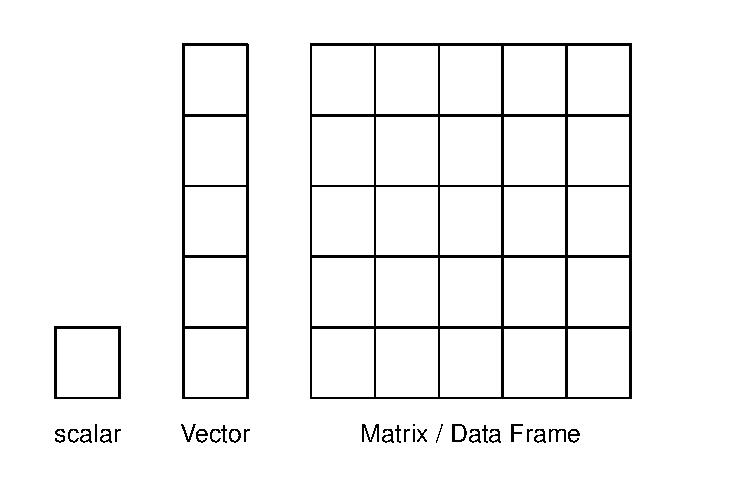
\includegraphics[width=\maxwidth]{figure/unnamed-chunk-97-1} 

\end{knitrout}
\end{tiny}
\label{fig:setfunctions}
\caption{Common set functions in R.}
\end{marginfigure}

\section{Using indexing to remove specific values of a vector}

Sometimes you might want to remove values of a vector before performing some analyses. This might be because some of the values are invalid or just not values that you want to include in your analyses. For example, let's say you asked 7 people how happy they were on a scale of 1 to 5 and received the following responses:

\begin{knitrout}
\definecolor{shadecolor}{rgb}{0.969, 0.969, 0.969}\color{fgcolor}\begin{kframe}
\begin{alltt}
\hlstd{happy} \hlkwb{<-} \hlkwd{c}\hlstd{(}\hlnum{1}\hlstd{,} \hlnum{4}\hlstd{,} \hlnum{2}\hlstd{,} \hlnum{999}\hlstd{,} \hlnum{2}\hlstd{,} \hlnum{3}\hlstd{,} \hlopt{-}\hlnum{2}\hlstd{)}
\end{alltt}
\end{kframe}
\end{knitrout}

As you can see, we have some invalid values (999 and -2) in this vector. We can use logical indexing to create a new vector called \texttt{happy.valid} that only contains values 1 through 5.

\begin{knitrout}
\definecolor{shadecolor}{rgb}{0.969, 0.969, 0.969}\color{fgcolor}\begin{kframe}
\begin{alltt}
\hlstd{valid.log} \hlkwb{<-} \hlstd{happy} \hlopt \hlkwd{c}\hlstd{(}\hlnum{1}\hlstd{,} \hlnum{2}\hlstd{,} \hlnum{3}\hlstd{,} \hlnum{4}\hlstd{,} \hlnum{5}\hlstd{)}
\hlstd{happy.valid} \hlkwb{<-} \hlstd{happy[valid.log]}
\hlstd{happy.valid}
\end{alltt}
\begin{verbatim}
## [1] 1 4 2 2 3
\end{verbatim}
\end{kframe}
\end{knitrout}

As you can see, the new vector \texttt{happy.valid} only contains values from the original vector that are integers from 1 to 5.

R has special functions for testing whether or not values in a dataset are either missing (or infinite). Here are some you can use:



  \vspace{5mm} %5mm vertical space
\noindent
\setlength{\fboxrule}{1.5pt}
\fbox{
\parbox{\textwidth}{

\newfun{Logical testing functions}

\hline

\begin{description}

\item[\tt{is.integer(x)}] \hfill \\
Tests if values in a vector are integers
\item[\tt{is.na(x), is.null(x)}] \hfill \\
Tests if values in a vector are \texttt{NA} or \texttt{NULL}
\item[\tt{is.finite(x)}] \hfill \\
 Tests if a value is a finite numerical value. If a value is NA, NULL, Inf, or -Inf, \texttt{is.finite()} will return \texttt{FALSE}.
\item[\tt{duplicated(x))}] \hfill \\
Returns \texttt{FALSE} at the first location of each unique value in x, and \texttt{TRUE} for all future locations of unique values. For example, \texttt{duplicated(c(1, 2, 1, 2, 3))} returns \texttt(FALSE, FALSE, TRUE, TRUE, FALSE). If you want to remove duplicated values from a vector, just run \texttt{x <- x[!duplicated(x)]}

\end{description}

}
}
\vspace{5mm} %5mm vertical space



  You can use these functions to generate logical indices for indexing. For example, let's say you had a vector of data with several missing values. To create a new vector of data that does not contain the original NA values, we can index the original \texttt{data} vector with \texttt{is.finite(data)}:

\begin{knitrout}
\definecolor{shadecolor}{rgb}{0.969, 0.969, 0.969}\color{fgcolor}\begin{kframe}
\begin{alltt}
\hlstd{data} \hlkwb{<-} \hlkwd{c}\hlstd{(}\hlnum{5}\hlstd{,} \hlnum{2}\hlstd{,} \hlnum{NA}\hlstd{,} \hlnum{3}\hlstd{,} \hlnum{NA}\hlstd{,} \hlnum{10}\hlstd{,} \hlnum{NA}\hlstd{)}
\hlstd{data.finite} \hlkwb{<-} \hlstd{data[}\hlkwd{is.finite}\hlstd{(data)]}
\hlstd{data.finite}
\end{alltt}
\begin{verbatim}
## [1]  5  2  3 10
\end{verbatim}
\end{kframe}
\end{knitrout}


\section{Taking the sum and mean of logical vectors to get counts and percentages}

Many (if not all) R functions that take numeric data as inputs will interpret TRUE values as 1 and FALSE values as 0. This allows us to easily answer questions like "How many values in a data vector are greater than 0?" or "What percentage of values are equal to 5?" by applying the \texttt{sum()} or \texttt{mean()} function to a logical vector.

Let's use this logic to see how many of the integers from 1 to 100 are greater than 0, 50, and 100:

\begin{knitrout}
\definecolor{shadecolor}{rgb}{0.969, 0.969, 0.969}\color{fgcolor}\begin{kframe}
\begin{alltt}
\hlkwd{sum}\hlstd{(}\hlnum{1}\hlopt{:}\hlnum{100} \hlopt{>} \hlnum{0}\hlstd{)} \hlcom{# How many values in 1:100 are greater than 0?}
\end{alltt}
\begin{verbatim}
## [1] 100
\end{verbatim}
\begin{alltt}
\hlkwd{sum}\hlstd{(}\hlnum{1}\hlopt{:}\hlnum{100} \hlopt{>} \hlnum{50}\hlstd{)} \hlcom{# How many values in 1:100 are greater than 50?}
\end{alltt}
\begin{verbatim}
## [1] 50
\end{verbatim}
\begin{alltt}
\hlkwd{sum}\hlstd{(}\hlnum{1}\hlopt{:}\hlnum{100} \hlopt{>} \hlnum{100}\hlstd{)} \hlcom{# How many values in 1:100 are greater than 50?}
\end{alltt}
\begin{verbatim}
## [1] 0
\end{verbatim}
\end{kframe}
\end{knitrout}

These results should make sense: every value from 1:100 is greater than 0, 50 are greater than 50, and non are greater than 100. Now, let's do the same thing but calculate percentages instead of counts using \texttt{mean()} instead of \texttt{sum()}:

\begin{knitrout}
\definecolor{shadecolor}{rgb}{0.969, 0.969, 0.969}\color{fgcolor}\begin{kframe}
\begin{alltt}
\hlkwd{mean}\hlstd{(}\hlnum{1}\hlopt{:}\hlnum{100} \hlopt{>} \hlnum{0}\hlstd{)} \hlcom{# How many values in 1:100 are greater than 0?}
\end{alltt}
\begin{verbatim}
## [1] 1
\end{verbatim}
\begin{alltt}
\hlkwd{mean}\hlstd{(}\hlnum{1}\hlopt{:}\hlnum{100} \hlopt{>} \hlnum{50}\hlstd{)} \hlcom{# How many values in 1:100 are greater than 50?}
\end{alltt}
\begin{verbatim}
## [1] 0.5
\end{verbatim}
\begin{alltt}
\hlkwd{mean}\hlstd{(}\hlnum{1}\hlopt{:}\hlnum{100} \hlopt{>} \hlnum{100}\hlstd{)} \hlcom{# How many values in 1:100 are greater than 50?}
\end{alltt}
\begin{verbatim}
## [1] 0
\end{verbatim}
\end{kframe}
\end{knitrout}

So far so good, now let's try this on our tattoo data:

\begin{knitrout}
\definecolor{shadecolor}{rgb}{0.969, 0.969, 0.969}\color{fgcolor}\begin{kframe}
\begin{alltt}
\hlstd{tattoos} \hlkwb{<-} \hlkwd{c}\hlstd{(}\hlnum{4}\hlstd{,} \hlnum{50}\hlstd{,} \hlnum{2}\hlstd{,} \hlnum{39}\hlstd{,} \hlnum{4}\hlstd{,} \hlnum{20}\hlstd{,} \hlnum{4}\hlstd{,} \hlnum{8}\hlstd{,} \hlnum{10}\hlstd{,} \hlnum{100}\hlstd{)}
\end{alltt}
\end{kframe}
\end{knitrout}

Let's see see how many of these 10 pirates have more than 10 tattoos. We'll do this in two steps; First, we'll create a logical vector indicating which values are greater than 10. Second, we'll take the sum of this logical vector. This will tell us how many \texttt{TRUE} values there are in the logical vector:

\begin{knitrout}
\definecolor{shadecolor}{rgb}{0.969, 0.969, 0.969}\color{fgcolor}\begin{kframe}
\begin{alltt}
\hlstd{log.vec} \hlkwb{<-} \hlstd{tattoos} \hlopt{>} \hlnum{10} \hlcom{# Step 1: Which values are > 10?}
\hlkwd{sum}\hlstd{(log.vec)} \hlcom{# Step 2: How many TRUE values are there?}
\end{alltt}
\begin{verbatim}
## [1] 4
\end{verbatim}
\end{kframe}
\end{knitrout}

Looks like 4 pirates have more than 10 tattoos. Now, let's test what percent of pirates have 5 tattoos or less. We'll do this by first creating the logical vector, and then calculating the \texttt{mean()} of this vector. We can do this because the mean of a vector of 0s and 1s is identical to the percentage of 1s:

\begin{knitrout}
\definecolor{shadecolor}{rgb}{0.969, 0.969, 0.969}\color{fgcolor}\begin{kframe}
\begin{alltt}
\hlstd{log.vec} \hlkwb{<-} \hlstd{tattoos} \hlopt{<=} \hlnum{5} \hlcom{# Step 1: Which values are <= 5?}
\hlkwd{mean}\hlstd{(log.vec)} \hlcom{# Step 2: What percent of values are TRUE?}
\end{alltt}
\begin{verbatim}
## [1] 0.4
\end{verbatim}
\end{kframe}
\end{knitrout}

Looks like 40\% of pirates have 5 tattoos or less.


\marginnote{To see what percentage of values are TRUE in a logical vector, just take the mean of the vector. For example, the command \texttt{mean(c(-1, -2, 1, 1) > 0)} will return \texttt{0.50}, telling you that half of the values are positive.}


\subsection{Additional Tips}

\begin{itemize}

  \item If you have a vector of values and you want to know which values are duplicates of previous values, you can use the \texttt{duplicated} function. This function will go through the vector from beginning to end and tag the first unique instance of a value as TRUE and all repeated instances of a value as FALSE:

\begin{knitrout}
\definecolor{shadecolor}{rgb}{0.969, 0.969, 0.969}\color{fgcolor}\begin{kframe}
\begin{alltt}
\hlstd{vec} \hlkwb{<-} \hlkwd{c}\hlstd{(}\hlstr{"a"}\hlstd{,} \hlstr{"b"}\hlstd{,} \hlstr{"a"}\hlstd{,} \hlstr{"a"}\hlstd{,} \hlstr{"c"}\hlstd{)}
\hlkwd{duplicated}\hlstd{(}\hlkwd{c}\hlstd{(}\hlstr{"a"}\hlstd{,} \hlstr{"b"}\hlstd{,} \hlstr{"a"}\hlstd{,} \hlstr{"a"}\hlstd{,} \hlstr{"c"}\hlstd{))}
\end{alltt}
\begin{verbatim}
## [1] FALSE FALSE  TRUE  TRUE FALSE
\end{verbatim}
\end{kframe}
\end{knitrout}

If you want to remove duplicated values from a vector, you can just index the vector by \texttt{!duplicated}:

\begin{knitrout}
\definecolor{shadecolor}{rgb}{0.969, 0.969, 0.969}\color{fgcolor}\begin{kframe}
\begin{alltt}
\hlstd{vec[}\hlopt{!}\hlkwd{duplicated}\hlstd{(vec)]}
\end{alltt}
\begin{verbatim}
## [1] "a" "b" "c"
\end{verbatim}
\end{kframe}
\end{knitrout}

However, you can do the same thing with \texttt{unique()}!


\end{itemize}


\section{A worked example - Chicken Weights}

A farmer is testing the effectiveness of three different diets on the weight gain of chickens. When they are born, 50 chicks are randomly assigned to one of 4 diets. Over several time periods, the farmer weighs each chicken. These data are contained in the dataset \texttt{ChickWeight}. Because the data are stored in a dataframe, which we haven't learned yet, we'll convert the four columns in the dataset to vectors as follows:

\begin{knitrout}
\definecolor{shadecolor}{rgb}{0.969, 0.969, 0.969}\color{fgcolor}\begin{kframe}
\begin{alltt}
\hlstd{weights} \hlkwb{<-} \hlstd{ChickWeight}\hlopt{$}\hlstd{weight}
\hlstd{time} \hlkwb{<-} \hlstd{ChickWeight}\hlopt{$}\hlstd{Time}
\hlstd{chick} \hlkwb{<-} \hlkwd{as.numeric}\hlstd{(}\hlkwd{paste}\hlstd{(ChickWeight}\hlopt{$}\hlstd{Chick))}
\hlstd{diet} \hlkwb{<-} \hlkwd{as.numeric}\hlstd{(ChickWeight}\hlopt{$}\hlstd{Diet)}
\end{alltt}
\end{kframe}
\end{knitrout}

Let's answer 5 questions with these vectors:

\begin{enumerate}

  \item What are the first 10 elements of the \texttt{weights} vector and the last 10 elements of the \texttt{weights} vector?\marginnote{To answer the second question, I used the \texttt{length()} function to index index \texttt{weights} to go from 9 elements \textit{before} the end of the vector, to the end of the vector.}

\begin{knitrout}
\definecolor{shadecolor}{rgb}{0.969, 0.969, 0.969}\color{fgcolor}\begin{kframe}
\begin{alltt}
\hlstd{weights[}\hlnum{1}\hlopt{:}\hlnum{10}\hlstd{]}
\end{alltt}
\begin{verbatim}
##  [1]  42  51  59  64  76  93 106 125 149 171
\end{verbatim}
\begin{alltt}
\hlstd{weights[(}\hlkwd{length}\hlstd{(weights)} \hlopt{-} \hlnum{9}\hlstd{)}\hlopt{:}\hlkwd{length}\hlstd{(weights)]}
\end{alltt}
\begin{verbatim}
##  [1]  67  84 105 122 155 175 205 234 264 264
\end{verbatim}
\end{kframe}
\end{knitrout}

  \item Which chicks were given diets 1 and 2?

\begin{knitrout}
\definecolor{shadecolor}{rgb}{0.969, 0.969, 0.969}\color{fgcolor}\begin{kframe}
\begin{alltt}
\hlkwd{unique}\hlstd{(chick[diet} \hlopt{==} \hlnum{1}\hlstd{])}
\end{alltt}
\begin{verbatim}
##  [1]  1  2  3  4  5  6  7  8  9 10 11 12 13 14 15 16 17 18 19 20
\end{verbatim}
\begin{alltt}
\hlkwd{unique}\hlstd{(chick[diet} \hlopt{==} \hlnum{2}\hlstd{])}
\end{alltt}
\begin{verbatim}
##  [1] 21 22 23 24 25 26 27 28 29 30
\end{verbatim}
\end{kframe}
\end{knitrout}

  \item What was the mean weight across all time periods separately for diets 3 and 4?\marginnote{First, I indexed the \texttt{weights} vector with a logical vector created from from \texttt{diet}. I then calculated the mean of this indexed vector.}

\begin{knitrout}
\definecolor{shadecolor}{rgb}{0.969, 0.969, 0.969}\color{fgcolor}\begin{kframe}
\begin{alltt}
\hlkwd{mean}\hlstd{(weights[diet} \hlopt{==} \hlnum{3}\hlstd{])}
\end{alltt}
\begin{verbatim}
## [1] 142.95
\end{verbatim}
\begin{alltt}
\hlkwd{mean}\hlstd{(weights[diet} \hlopt{==} \hlnum{4}\hlstd{])}
\end{alltt}
\begin{verbatim}
## [1] 135.2627
\end{verbatim}
\end{kframe}
\end{knitrout}

  \item What was the standard deviation of weights for diets 1 and 2 at time < 10?

\begin{knitrout}
\definecolor{shadecolor}{rgb}{0.969, 0.969, 0.969}\color{fgcolor}\begin{kframe}
\begin{alltt}
\hlkwd{sd}\hlstd{(weights[diet} \hlopt{<=} \hlnum{2} \hlopt{&} \hlstd{time} \hlopt{<} \hlnum{10}\hlstd{])}
\end{alltt}
\begin{verbatim}
## [1] 17.2321
\end{verbatim}
\end{kframe}
\end{knitrout}

  \item What was the median weight for chicks 10, 20, and 30 for time periods greater than 10?

\begin{knitrout}
\definecolor{shadecolor}{rgb}{0.969, 0.969, 0.969}\color{fgcolor}\begin{kframe}
\begin{alltt}
\hlkwd{median}\hlstd{(weights[chick} \hlopt \hlkwd{c}\hlstd{(}\hlnum{10}\hlstd{,} \hlnum{20}\hlstd{,} \hlnum{30}\hlstd{)} \hlopt{&} \hlstd{time} \hlopt{>} \hlnum{10}\hlstd{])}
\end{alltt}
\begin{verbatim}
## [1] 115
\end{verbatim}
\end{kframe}
\end{knitrout}

  \item Which chicks did not make it until the final time period?\marginnote{This one is a bit tricky. First, I need a vector of all chicks in the study (\texttt{all.chicks}). Next, I need a vector of all chicks that survived to the last time point (\texttt{surviving.chicks}). Third, I need to test, for each chick, whether they are present in the vector of surviving chicks (\texttt{survived.log}). Finally, I index the vector of all chicks where the logical index is FALSE (because we want chicks that did not survive).}

\begin{knitrout}
\definecolor{shadecolor}{rgb}{0.969, 0.969, 0.969}\color{fgcolor}\begin{kframe}
\begin{alltt}
\hlcom{# Step 1: Create a vector of all chicks (all.chicks)}
\hlstd{all.chicks} \hlkwb{<-} \hlkwd{sort}\hlstd{(}\hlkwd{unique}\hlstd{(chick))}

\hlcom{#Step 2: Create a vector of all chicks that survive until the end (surviving.chicks)}
\hlstd{surviving.chicks} \hlkwb{<-} \hlkwd{sort}\hlstd{(}\hlkwd{unique}\hlstd{(chick[time} \hlopt{==} \hlkwd{max}\hlstd{(time)]))}

\hlcom{# Step 3: For each chick, see if it is present in the vector of surviving chicks}
\hlstd{survived.log} \hlkwb{<-} \hlstd{all.chicks} \hlopt \hlstd{surviving.chicks}

\hlcom{# Step 4: Index the vector of all chicks by the logical vector}
\hlstd{all.chicks[survived.log} \hlopt{==} \hlnum{FALSE}\hlstd{]}
\end{alltt}
\begin{verbatim}
## [1]  8 15 16 18 44
\end{verbatim}
\end{kframe}
\end{knitrout}

\end{enumerate}


\section{Test your R might!}

The following vour vectors give data about 10 movies.

\begin{knitrout}
\definecolor{shadecolor}{rgb}{0.969, 0.969, 0.969}\color{fgcolor}\begin{kframe}
\begin{alltt}
\hlstd{m.names} \hlkwb{<-} \hlkwd{c}\hlstd{(}\hlstr{"Baramgwa hamjje sarajida"}\hlstd{,} \hlstr{"Sleepless in Seattle"}\hlstd{,} \hlstr{"The Water Diviner"}\hlstd{,}
\hlstr{"Fly Away Home"}\hlstd{,} \hlstr{"The Three Musketeers"}\hlstd{,} \hlstr{"Candyman: Farewell to Flesh"}\hlstd{,}
\hlstr{"Honey I Threw our Kid off the Plank"}\hlstd{,} \hlstr{"Kingsman: The Secret Service"}\hlstd{,} \hlstr{"Ajab Prem Ki Ghazab Kahani"}\hlstd{,}
\hlstr{"A Bug's Life"}\hlstd{)}

\hlstd{boxoffice} \hlkwb{<-} \hlkwd{c}\hlstd{(}\hlnum{28686545}\hlstd{,} \hlnum{218076024}\hlstd{,} \hlnum{30864649}\hlstd{,} \hlnum{35870837}\hlstd{,} \hlnum{50375628}\hlstd{,} \hlnum{13899536}\hlstd{,}
\hlnum{58662452}\hlstd{,} \hlnum{404561724}\hlstd{,} \hlnum{15906411}\hlstd{,} \hlnum{363089431}\hlstd{)}

\hlstd{genre} \hlkwb{<-} \hlkwd{c}\hlstd{(}\hlstr{"Action"}\hlstd{,} \hlstr{"Romantic Comedy"}\hlstd{,} \hlstr{"Drama"}\hlstd{,} \hlstr{"Drama"}\hlstd{,} \hlstr{"Adventure"}\hlstd{,}
\hlstr{"Horror"}\hlstd{,} \hlstr{"Comedy"}\hlstd{,} \hlstr{"Action"}\hlstd{,} \hlstr{"Comedy"}\hlstd{,} \hlstr{"Adventure"}\hlstd{)}

\hlstd{time} \hlkwb{<-} \hlkwd{c}\hlstd{(}\hlnum{121}\hlstd{,} \hlnum{100}\hlstd{,} \hlnum{112}\hlstd{,} \hlnum{NA}\hlstd{,} \hlnum{NA}\hlstd{,} \hlnum{NA}\hlstd{,} \hlnum{NA}\hlstd{,} \hlnum{129}\hlstd{,} \hlnum{NA}\hlstd{,} \hlnum{96}\hlstd{)}

\hlstd{rating} \hlkwb{<-} \hlkwd{c}\hlstd{(}\hlnum{NA}\hlstd{,} \hlstr{"PG"}\hlstd{,} \hlstr{"R"}\hlstd{,} \hlstr{"PG"}\hlstd{,} \hlstr{"PG"}\hlstd{,} \hlstr{"R"}\hlstd{,} \hlstr{"PG"}\hlstd{,} \hlstr{"R"}\hlstd{,} \hlnum{NA}\hlstd{,} \hlstr{"G"}\hlstd{)}
\end{alltt}
\end{kframe}
\end{knitrout}

\begin{enumerate}

  \item What is the name of the 10th movie?
  
  \item What are the genres of the first 4 movies?
  
  \item What are the names of every second movie? (that is, the 2nd, 4th, 6th, 8th, and 10th).
  
  \item Some joker changed the name of the Pixar film "A Bug's Life" to "A Pirate's Life." Please correct the name of this movie.
  
  \item Create a new vector called “boxoffice.millions” that has the box-office values in millions of dollars. For example, a value of 1000000 in the original boxoffice vector should be 1 in boxoffice.millions
  
  \item What is the mean, median, and standard deviation of the box-office totals of all movies?
  
  \item What where the different movie genres and how many movies are there of each genre? (hint: use table())
  
  \item How many movies were Dramas? (hint: don't use table(), use sum())
  
  \item What was the box-office total, genre, running time, and rating of "A Bug's Life"?. Do this once using numerical indexing and once using logical indexing.
  
  \item What were the names of the movies that made less than \$30 Million dollars AND were Comedies?


\end{enumerate}


%----------------------------------------------------------------------------------------
%	CHAPTER 5
%----------------------------------------------------------------------------------------

\chapter{5: Matrices and Data Frames}}
\label{ch:5}


Chapter Goals


\begin{enumerate}
  \item Learn about the matrix and dataframe data objects
  \item Create matrices with matrix(), cbind(), and data.frame()
  \item Index matrices/dataframes with brackets [], and \$
  \item Use matrix/dataframe functions dim(), nrow(), ncol(), head(), tail()
  \item Import datasets
\end{enumerate}


\section{Creating matrices and dataframes}

By now, you should be comfortable with scalars and vectors. Next, we'll cover the next two most common data objects in R, \textbf{matrices} and \textbf{dataframes}

Matrices and dataframes are both two dimensional objects that contain rows and columns. Really, they're just like spreadsheets in Excel. Each matrix or dataframe contains a certain number of rows (call that number m) and columns (n). You can think of a matrix as a combination of n vectors, where each vector has a length of m. See Figure \ref{fig:scalarvectormatrix} to see the difference.


\begin{marginfigure}
\begin{tiny}
\begin{knitrout}
\definecolor{shadecolor}{rgb}{0.969, 0.969, 0.969}\color{fgcolor}\begin{kframe}
\begin{alltt}
\hlcom{# scalar v vector v matrix}

\hlkwd{par}\hlstd{(}\hlkwc{mar} \hlstd{=} \hlkwd{rep}\hlstd{(}\hlnum{1}\hlstd{,} \hlnum{4}\hlstd{))}
\hlkwd{plot}\hlstd{(}\hlnum{1}\hlstd{,} \hlkwc{xlim} \hlstd{=} \hlkwd{c}\hlstd{(}\hlnum{0}\hlstd{,} \hlnum{10}\hlstd{),} \hlkwc{ylim} \hlstd{=} \hlkwd{c}\hlstd{(}\hlopt{-}\hlnum{.5}\hlstd{,} \hlnum{5}\hlstd{),}
     \hlkwc{xlab} \hlstd{=} \hlstr{""}\hlstd{,} \hlkwc{ylab} \hlstd{=} \hlstr{""}\hlstd{,}
     \hlkwc{xaxt} \hlstd{=} \hlstr{"n"}\hlstd{,} \hlkwc{yaxt} \hlstd{=} \hlstr{"n"}\hlstd{,}
     \hlkwc{bty} \hlstd{=} \hlstr{"n"}\hlstd{,} \hlkwc{type} \hlstd{=} \hlstr{"n"}\hlstd{)}

\hlcom{# scalar}
\hlkwd{rect}\hlstd{(}\hlkwd{rep}\hlstd{(}\hlnum{0}\hlstd{,} \hlnum{1}\hlstd{),} \hlkwd{rep}\hlstd{(}\hlnum{0}\hlstd{,} \hlnum{1}\hlstd{),} \hlkwd{rep}\hlstd{(}\hlnum{1}\hlstd{,} \hlnum{1}\hlstd{),} \hlkwd{rep}\hlstd{(}\hlnum{1}\hlstd{,} \hlnum{1}\hlstd{))}
\hlkwd{text}\hlstd{(}\hlnum{.5}\hlstd{,} \hlopt{-}\hlnum{.5}\hlstd{,} \hlstr{"scalar"}\hlstd{)}

\hlcom{# Vector}
\hlkwd{rect}\hlstd{(}\hlkwd{rep}\hlstd{(}\hlnum{2}\hlstd{,} \hlnum{5}\hlstd{),} \hlnum{0}\hlopt{:}\hlnum{4}\hlstd{,} \hlkwd{rep}\hlstd{(}\hlnum{3}\hlstd{,} \hlnum{5}\hlstd{),} \hlnum{1}\hlopt{:}\hlnum{5}\hlstd{)}
\hlkwd{text}\hlstd{(}\hlnum{2.5}\hlstd{,} \hlopt{-}\hlnum{.5}\hlstd{,} \hlstr{"Vector"}\hlstd{)}

\hlcom{# Matrix}
\hlkwd{rect}\hlstd{(}\hlkwd{rep}\hlstd{(}\hlnum{4}\hlopt{:}\hlnum{8}\hlstd{,} \hlkwc{each} \hlstd{=} \hlnum{5}\hlstd{),}
     \hlkwd{rep}\hlstd{(}\hlnum{0}\hlopt{:}\hlnum{4}\hlstd{,} \hlkwc{times} \hlstd{=} \hlnum{5}\hlstd{),}
     \hlkwd{rep}\hlstd{(}\hlnum{5}\hlopt{:}\hlnum{9}\hlstd{,} \hlkwc{each} \hlstd{=} \hlnum{5}\hlstd{),}
     \hlkwd{rep}\hlstd{(}\hlnum{1}\hlopt{:}\hlnum{5}\hlstd{,} \hlkwc{times} \hlstd{=} \hlnum{5}\hlstd{))}
\hlkwd{text}\hlstd{(}\hlnum{6.5}\hlstd{,} \hlopt{-}\hlnum{.5}\hlstd{,} \hlstr{"Matrix / Data Frame"}
     \hlstd{)}
\end{alltt}
\end{kframe}
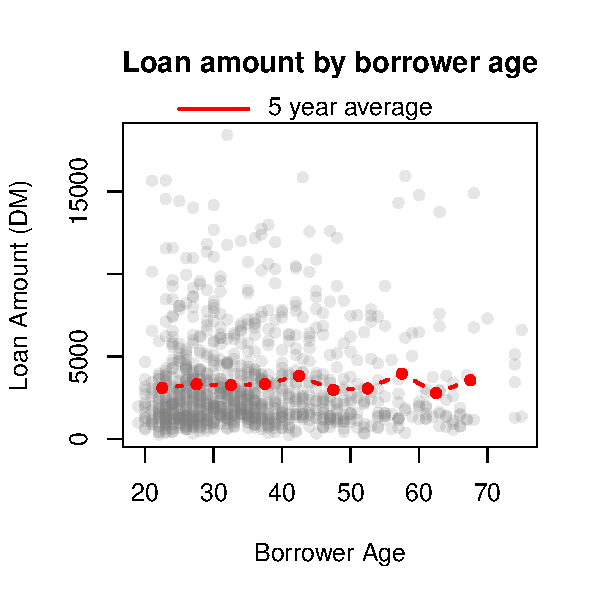
\includegraphics[width=\maxwidth]{figure/unnamed-chunk-116-1} 

\end{knitrout}
\caption{scalar, Vector, Matrix... ::drops mike::}
\label{fig:scalarvectormatrix}
\end{tiny}
\end{marginfigure}

You can use several functions in R to create matrices and dataframes. In the next sections we'll cover the most common ones.

\subsection{cbind() and rbind()}

\texttt{cbind()} and \texttt{rbind()} both create matrices by combining several vectors together into a single matrix. cbind() combines vectors as columns in the matrix, while rbind() combines them as rows.



\vspace{5mm} %5mm vertical space
\noindent
\setlength{\fboxrule}{1.5pt}
\fbox{
\parbox{\textwidth}{

\newfun{cbind(), rbind()}\index{cbind()}\index{rbind()}

\hline

\begin{description}

  \item[\tt{x, y, ...}] \hfill \\
      One or more vectors to be combined into a matrix
\end{description}

}
}
\vspace{5mm} %5mm vertical space

Let's use these functions to create a matrix with the numbers 1 through 30. First, we'll create three vectors of length 10, then we'll combine them into one matrix.

\begin{footnotesize}
\begin{knitrout}
\definecolor{shadecolor}{rgb}{0.969, 0.969, 0.969}\color{fgcolor}\begin{kframe}
\begin{alltt}
\hlstd{x} \hlkwb{<-} \hlnum{1}\hlopt{:}\hlnum{10}
\hlstd{y} \hlkwb{<-} \hlnum{11}\hlopt{:}\hlnum{20}
\hlstd{z} \hlkwb{<-} \hlnum{21}\hlopt{:}\hlnum{30}

\hlstd{matrix.1} \hlkwb{<-} \hlkwd{rbind}\hlstd{(x, y, z)}
\hlstd{matrix.1}
\end{alltt}
\begin{verbatim}
##   [,1] [,2] [,3] [,4] [,5] [,6] [,7] [,8] [,9] [,10]
## x    1    2    3    4    5    6    7    8    9    10
## y   11   12   13   14   15   16   17   18   19    20
## z   21   22   23   24   25   26   27   28   29    30
\end{verbatim}
\begin{alltt}
\hlstd{matrix.2} \hlkwb{<-} \hlkwd{cbind}\hlstd{(x, y, z)}
\hlstd{matrix.2}
\end{alltt}
\begin{verbatim}
##        x  y  z
##  [1,]  1 11 21
##  [2,]  2 12 22
##  [3,]  3 13 23
##  [4,]  4 14 24
##  [5,]  5 15 25
##  [6,]  6 16 26
##  [7,]  7 17 27
##  [8,]  8 18 28
##  [9,]  9 19 29
## [10,] 10 20 30
\end{verbatim}
\end{kframe}
\end{knitrout}
\end{footnotesize}

As you can see, the \texttt{rbind()} function combined the vectors as rows in the final matrix, while the \texttt{cbind()} function combined them as columns.

If you want to create a matrix from a single vector of data, you can do this using the \texttt{matrix()} function.


\vspace{5mm} %5mm vertical space
\noindent
\setlength{\fboxrule}{1.5pt}
\fbox{
\parbox{\textwidth}{

\newfun{matrix()}\index{matrix()}

\hline

\begin{description}

  \item[\tt{data}] \hfill \\
      A vector of data
        \item[\tt{nrow}] \hfill \\
      The number of rows in the final matrix
        \item[\tt{ncol}] \hfill \\
      The number of columns in the final matrix
        \item[\tt{byrow}] \hfill \\
      A logical value indicating whether to fill the matrix by row or column
\end{description}

}
}
\vspace{5mm} %5mm vertical space


Let's use the \texttt{matrix()} function to re-create a matrix containing the values from 1 to 30.

\begin{footnotesize}
\begin{knitrout}
\definecolor{shadecolor}{rgb}{0.969, 0.969, 0.969}\color{fgcolor}\begin{kframe}
\begin{alltt}
\hlstd{matrix.1} \hlkwb{<-} \hlkwd{matrix}\hlstd{(}\hlkwc{data} \hlstd{=} \hlnum{1}\hlopt{:}\hlnum{30}\hlstd{,}
                   \hlkwc{nrow} \hlstd{=} \hlnum{10}\hlstd{,}
                   \hlkwc{ncol} \hlstd{=} \hlnum{3}\hlstd{)}
\hlstd{matrix.1}
\end{alltt}
\begin{verbatim}
##       [,1] [,2] [,3]
##  [1,]    1   11   21
##  [2,]    2   12   22
##  [3,]    3   13   23
##  [4,]    4   14   24
##  [5,]    5   15   25
##  [6,]    6   16   26
##  [7,]    7   17   27
##  [8,]    8   18   28
##  [9,]    9   19   29
## [10,]   10   20   30
\end{verbatim}
\begin{alltt}
\hlstd{matrix.2} \hlkwb{<-} \hlkwd{matrix}\hlstd{(}\hlkwc{data} \hlstd{=} \hlnum{1}\hlopt{:}\hlnum{30}\hlstd{,}
                   \hlkwc{nrow} \hlstd{=} \hlnum{3}\hlstd{,}
                   \hlkwc{ncol} \hlstd{=} \hlnum{10}\hlstd{)}
\hlstd{matrix.2}
\end{alltt}
\begin{verbatim}
##      [,1] [,2] [,3] [,4] [,5] [,6] [,7] [,8] [,9] [,10]
## [1,]    1    4    7   10   13   16   19   22   25    28
## [2,]    2    5    8   11   14   17   20   23   26    29
## [3,]    3    6    9   12   15   18   21   24   27    30
\end{verbatim}
\end{kframe}
\end{knitrout}
\end{footnotesize}

Keep in mind that matrices can either contain numbers or characters. If you try to create a matrix with both numbers and characters, it will turn all the numbers into characters:

\begin{footnotesize}
\begin{knitrout}
\definecolor{shadecolor}{rgb}{0.969, 0.969, 0.969}\color{fgcolor}\begin{kframe}
\begin{alltt}
\hlkwd{cbind}\hlstd{(}\hlnum{1}\hlopt{:}\hlnum{5}\hlstd{,} \hlkwd{c}\hlstd{(}\hlstr{"a"}\hlstd{,} \hlstr{"b"}\hlstd{,} \hlstr{"c"}\hlstd{,} \hlstr{"d"}\hlstd{,} \hlstr{"e"}\hlstd{))}
\end{alltt}
\begin{verbatim}
##      [,1] [,2]
## [1,] "1"  "a" 
## [2,] "2"  "b" 
## [3,] "3"  "c" 
## [4,] "4"  "d" 
## [5,] "5"  "e"
\end{verbatim}
\end{kframe}
\end{knitrout}
\end{footnotesize}

\subsection{Dataframe: An m x n object containing numbers, strings and factors}

A dataframe looks a lot like a matrix at first: it is also rectangular and has m rows and n columns. However, unlike matrices, dataframes can contain *both* string vectors and numeric vectors within the same object. For this reason, most large datasets in R, for example, a survey including numeric data and text data, will be stored as dataframes.

\marginnote{A dataframe is just a more flexible matrix that allows you to combine both character and numeric vectors into the same data object. Because dataframes are more flexible than matrices, Most datafiles you use will be stored as dataframes.}

\newfun{data.frame()}\index{data.frame()}

To create a dataframe, you can use the \texttt{data.frame()} function.To use the \texttt{data.frame()} function, start by defining the name of a column as a string (for example, \texttt{"gender"}), then indicate the contents of the column as a vector. You can add as many columns as you would like.

Let's create a dataframe of fictional survey data. I'll add a column called \texttt{initials} with a string vector indicating the person's first and last initials. I'll then add a \texttt{gender} column with 5 string values. I'll then add a column called \texttt{"height"} with five height values, and a column called \texttt{"siblings"} with 5 integer values indicating how many siblings each person has. Finally, I'll add the argument \texttt{stringsAsFactors = F}. This tells R to interpret strings as strings, and not as Factors, which are a different datatype that we don't want to deal with just yet.

\begin{footnotesize}
\begin{knitrout}
\definecolor{shadecolor}{rgb}{0.969, 0.969, 0.969}\color{fgcolor}\begin{kframe}
\begin{alltt}
\hlstd{survey} \hlkwb{<-} \hlkwd{data.frame}\hlstd{(}
          \hlstr{"initials"} \hlstd{=} \hlkwd{c}\hlstd{(}\hlstr{"MP"}\hlstd{,} \hlstr{"HT"}\hlstd{,} \hlstr{"RH"}\hlstd{,} \hlstr{"AP"}\hlstd{,} \hlstr{"NP"}\hlstd{),}
           \hlstr{"gender"} \hlstd{=} \hlkwd{c}\hlstd{(}\hlstr{"F"}\hlstd{,} \hlstr{"F"}\hlstd{,} \hlstr{"F"}\hlstd{,} \hlstr{"M"}\hlstd{,} \hlstr{"M"}\hlstd{),}
           \hlstr{"height"} \hlstd{=} \hlkwd{c}\hlstd{(}\hlnum{132}\hlstd{,} \hlnum{150}\hlstd{,} \hlnum{167}\hlstd{,} \hlnum{148}\hlstd{,} \hlnum{172}\hlstd{),}
           \hlstr{"siblings"} \hlstd{=} \hlkwd{c}\hlstd{(}\hlnum{0}\hlstd{,} \hlnum{2}\hlstd{,} \hlnum{0}\hlstd{,} \hlnum{1}\hlstd{,} \hlnum{2}\hlstd{),}
           \hlkwc{stringsAsFactors} \hlstd{= F} \hlcom{# don't convert strings to factors}
          \hlstd{)}

\hlstd{survey} \hlcom{# Print the dataframe}
\end{alltt}
\begin{verbatim}
##   initials gender height siblings
## 1       MP      F    132        0
## 2       HT      F    150        2
## 3       RH      F    167        0
## 4       AP      M    148        1
## 5       NP      M    172        2
\end{verbatim}
\end{kframe}
\end{knitrout}
\end{footnotesize}


\section{Data sets pre-loaded in R}

Until now, we've used the functions \texttt{matrix()} and \texttt{dataframe()} to manually create our own datasets within R. However, for demonstration purposes, it's frequently easier to use existing datasets. Thankfully, R has us covered: R has several datasets that come pre-installed in a package called \texttt{datasets}. While you probably won't make any major scientific discoveries with these datasets, they allow all R users to test and compare code on the same sets of data.\marginnote{To see a complete list of all the datasets included in the \texttt{datasets} package, run the code: \texttt{library(help = "datasets")}} Here are a few datasets that we will be using in future examples:

\begin{itemize}
  \item \texttt{ChickWeight}: Weight versus age of chicks on four different diets
  \item \texttt{InsectSprays}: Effectiveness of six different types of insect sprays
  \item \texttt{ToothGrowth}: The effects of different levels of vitamin C on the tooth growth of guinea pigs.
\end{itemize}

Since these datasets are preloaded in R, you can always access them by by name. We'll use them in the following examples.


\section{Getting information about matrices and dataframes}

When you are working with dataframes, you will frequently want to know its general attributes, such as the number of rows and columns it has. Here are some common functions to get basic information about a dataframe. For each of these functions, I'll use the label df to refer to the dataframe object:


\vspace{5mm} %5mm vertical space
\noindent
\setlength{\fboxrule}{1.5pt}
\fbox{
\parbox{\textwidth}{

\newfun{Helpful Dataframe Functions}

\hline

\begin{description}

\item[\tt{head(df), tail(df)}] \hfill \\
Look at the first few rows (head()) or the last few rows (tail()) of a dataframe in the console.

\item[\tt{View(df)}] \hfill \\
View the entire dataframe in a spreadsheet-like object. Make sure to use a capital V or the function won't work!

\item[\tt{dim(df), nrow(df), ncol(df)}] \hfill \\
Return information about the dimensions of the dataframe. dim() returns the number of rows and columns, while nrow() and ncol() return just the number of rows or columns.

\item[\tt{names(df)}] \hfill \\
Returns a string vector showing the names in the dataframe.

\item[\tt{summary(df)}] \hfill \\
Returns summary information about all columns in the dataframe. For numeric columns, you'll see basic summary statistics like the minimum, mean, maximum etc.

\item[\tt{str(df)}] \hfill \\
Tells you the structure of the dataframe - with information about the column names, the data class of each column (e.g.; numeric or string), and the first few cases in each column


\end{description}

}
}
\vspace{5mm} %5mm vertical space

Let's use some of these functions on the \texttt{ChickWeight} dataframe:

\newfun{names(df)}\index{names()}

The \texttt{names()} function will tell you the names of the columns in a dataframe. Let's use the function to see the columns in \texttt{ChickWeight}:

\begin{knitrout}
\definecolor{shadecolor}{rgb}{0.969, 0.969, 0.969}\color{fgcolor}\begin{kframe}
\begin{alltt}
\hlkwd{names}\hlstd{(ChickWeight)}
\end{alltt}
\begin{verbatim}
## [1] "weight" "Time"   "Chick"  "Diet"
\end{verbatim}
\end{kframe}
\end{knitrout}


\newfun{head(df)}\index{head()}

The function \texttt{head(x)} will show you the first few rows of a matrix / dataframe. Personally, I am constantly using this function to make sure that I didn't screw up a dataset when I'm working on it. Let's look at the first few rows of the dataframe \texttt{ChickWeight}, which contains data on the growth of chickens on several different diets.

\begin{knitrout}
\definecolor{shadecolor}{rgb}{0.969, 0.969, 0.969}\color{fgcolor}\begin{kframe}
\begin{alltt}
\hlkwd{head}\hlstd{(ChickWeight)}
\end{alltt}
\begin{verbatim}
##   weight Time Chick Diet
## 1     42    0     1    1
## 2     51    2     1    1
## 3     59    4     1    1
## 4     64    6     1    1
## 5     76    8     1    1
## 6     93   10     1    1
\end{verbatim}
\end{kframe}
\end{knitrout}

The \texttt{head()} function only shows you the first few rows of a dataframe, but usually this is enough to get a visual sense of the names of the dataframe, the number of columns, and the type of data in each column. But what if you want to see all values? You could print the entire dataframe into the console, but the console isn't a very friendly environment to view data. Instead, you can use the \texttt{View()} function, which will print the entire dataframe into a spreadsheet-like window:

\newfun{View(df)}\index{View()}

Let's use the \texttt{View()} function to look at the entire \texttt{ToothGrowth} dataframe:

\begin{knitrout}
\definecolor{shadecolor}{rgb}{0.969, 0.969, 0.969}\color{fgcolor}\begin{kframe}
\begin{alltt}
\hlkwd{View}\hlstd{(ToothGrowth)}
\end{alltt}
\end{kframe}
\end{knitrout}

When you run this code, you should see a separate window open (see Figure~\ref{fig:toothgrowthscreenshot}). You can use this window to scroll through the data, sort it via column values (by clicking on the column name), and even apply filters using the filter button on the top left of the screen. However, keep in mind that anything you do in the \texttt{View()} window will \textit{not} change the actual dataframe in any way. You cannot add or remove data using the window, and any sorting or filtering you apply won't be replicated in the actual data.

\begin{figure}[h]
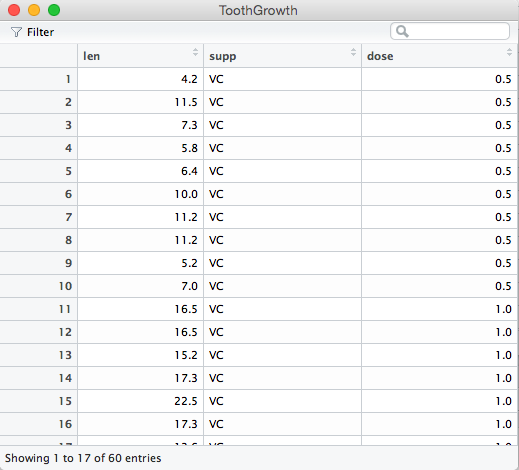
\includegraphics[width=10cm,keepaspectration]{/Users/Nathaniel/Dropbox/Git/YaRrr_Book/media/toothgrowthscreenshot.png}
\label{fig:toothgrowthscreenshot}
\caption{Screenshot of the window from \texttt{View(ToothGrowth)}. You can use this window to visually sort and filter the data to get an idea of how it looks, but you can't add or remove data and nothing you do will actually change the dataframe.}
\end{figure}


\newfun{dim(df), nrow(df), ncol(df)}

The \texttt{dim(), nrow()} and \texttt{ncol()} functions will give you information about the dimensions of the dataframe:
\begin{knitrout}
\definecolor{shadecolor}{rgb}{0.969, 0.969, 0.969}\color{fgcolor}\begin{kframe}
\begin{alltt}
\hlkwd{dim}\hlstd{(ChickWeight)}
\end{alltt}
\begin{verbatim}
## [1] 578   4
\end{verbatim}
\begin{alltt}
\hlkwd{nrow}\hlstd{(ChickWeight)}
\end{alltt}
\begin{verbatim}
## [1] 578
\end{verbatim}
\begin{alltt}
\hlkwd{ncol}\hlstd{(ChickWeight)}
\end{alltt}
\begin{verbatim}
## [1] 4
\end{verbatim}
\end{kframe}
\end{knitrout}



\section{Loading data into R with read.table()}

So far we've used either randomly generated data, or datasets pre-loaded in R. But how do you get an existing dataset into R? For the most part, getting datasets into R isn't that tricky - but only if your data is already in a 'nice' format. By 'nice,' I mean a text file with tab (or comma) separated columns. If your data is in another format (like Excel or Shitty Piece of Shitty Shit), I strongly recommend first exporting the data to a tab-delimited text file, and only then loading the data into R. That said, if for some reason you absolutely have to load a non-text file into R, look at the \textit{Additional Tips} sections for instructions.\marginnote{Import data into R as comma or tab-delimited text files whenever possible. If you need to load data in another format (e.g.; Excel), save it as a text file from the original program first.}

Once you have a text file, you can load it into R using the \texttt{read.table()} function. To use the \texttt{read.table()} function, you need to know where the text file is located on your computer. To do this, find the file on your harddrive then right-click it and view its properties. You should be able to see its file-path there. For example, the file path of a text file called \texttt{mydata} on my desktop is \texttt{"Users/Nathaniel/Desktop/mydata.txt"}.

Here are the main arguments to \texttt{read.table()} (to see all of them, run \texttt{?read.table})



\vspace{5mm} %5mm vertical space
\noindent
\setlength{\fboxrule}{1.5pt}
\fbox{
\parbox{\textwidth}{

\newfun{read.table()}\index{read.table()}

\hline

\begin{description}

  \item[\tt{file}] \hfill \\
      The document's file path (make sure to enter as a string with quotation marks!) OR an html link to a file.
        \item[\tt{header}] \hfill \\
      A logical value indicating whether the data has a header row or not.
        \item[\tt{ncol}] \hfill \\
      The number of columns in the final matrix
        \item[\tt{sep}] \hfill \\
      A string indicating how the columns are separated. For comma separated files, use \texttt{","}, for tab-delimited files, use \texttt{"\textbackslash t"}
      \item[\tt{stringsAsFactors}] \hfill \\
     A logical value indicating whether or not to convert strings to factors. I always set this to FALSE (because I don't like using factors)
\end{description}

}
}
\vspace{5mm} %5mm vertical space


To test this function, let's read in the datafile called \texttt{pirates.txt}. This datafile contains data from a survey of 1,000 pirates at the 2015 annual pirate meeting at the Bodensee in Konstanz, Germany. You can access this data in one of two ways: First, you can download this file from: http://nathanieldphillips.com/wp-content/uploads/2015/11/pirates1.txt) and a note of its directory on your computer (on my computer, the path is \texttt{/Users/Nathaniel/Dropbox/Public/pirates.txt}). You can then load the data into R by using \texttt{read.table}:

\vspace{5mm}
\begin{minipage}{16cm}
\begin{footnotesize}
\begin{knitrout}
\definecolor{shadecolor}{rgb}{0.969, 0.969, 0.969}\color{fgcolor}\begin{kframe}
\begin{alltt}
\hlstd{pirate.survey} \hlkwb{<-} \hlkwd{read.table}\hlstd{(}\hlkwc{file} \hlstd{=} \hlstr{"/Users/Nathaniel/Dropbox/Public/pirates.txt"}\hlstd{,}
                      \hlkwc{header} \hlstd{= T,}
                      \hlkwc{sep} \hlstd{=} \hlstr{"\textbackslash{}t"}\hlstd{,} \hlcom{# tab-delimited}
                      \hlkwc{stringsAsFactors} \hlstd{= F}
                      \hlstd{)}
\end{alltt}
\end{kframe}
\end{knitrout}
\end{footnotesize}
\caption{Loading a dataset from a text file.}
\end{minipage}
\vspace{5mm}

If you receive an error, it's probably because you entered the file path incorrectly. One trick to get the file path easily is by using RStudio's \textbf{Import Dataset} menu (see \textit{Additional Tips}). If you got the directory location correct, and the file exists, then you should not receive any error warning after executing \texttt{read.table()}.

Alternatively, you can load the dataset directly into R by entering the HTML link as the \texttt{file} argument to \texttt{read.table}



\vspace{5mm}
\begin{minipage}{16cm}
\begin{footnotesize}
\begin{knitrout}
\definecolor{shadecolor}{rgb}{0.969, 0.969, 0.969}\color{fgcolor}\begin{kframe}
\begin{alltt}
\hlstd{pirate.survey} \hlkwb{<-} \hlkwd{read.table}\hlstd{(}\hlkwc{file} \hlstd{=} \hlstr{"http://nathanieldphillips.com/wp-content/uploads/2015/11/pirates1.txt"}\hlstd{,}
                      \hlkwc{header} \hlstd{= T,}
                      \hlkwc{sep} \hlstd{=} \hlstr{"\textbackslash{}t"}\hlstd{,} \hlcom{# tab-delimited}
                      \hlkwc{stringsAsFactors} \hlstd{= F}
                      \hlstd{)}
\end{alltt}
\end{kframe}
\end{knitrout}
\end{footnotesize}
\caption{Loading a data set from a URL link}
\end{minipage}
\vspace{5mm}

The data is now stored as a dataframe and you can now access it via the object name you assigned it to (in my case, I called it \texttt{Flights}). To make sure it loaded correctly, try seeing the first few rows with \texttt{head()}

\vspace{5mm}
\begin{minipage}{18cm}
\begin{footnotesize}
\begin{knitrout}
\definecolor{shadecolor}{rgb}{0.969, 0.969, 0.969}\color{fgcolor}\begin{kframe}
\begin{alltt}
\hlkwd{head}\hlstd{(pirate.survey)}
\end{alltt}
\begin{verbatim}
##   id    sex headband age college tattoos tchests parrots favorite.pirate
## 1  1 female      yes  30   JSSFP      11      20       7      Blackbeard
## 2  2   male      yes  25    CCCC      15       6       3        Anicetus
## 3  3   male      yes  25    CCCC      12       5       2    Jack Sparrow
## 4  4   male      yes  29   JSSFP      12       0       1      Edward Low
## 5  5 female      yes  31    CCCC      17      11      10        Anicetus
## 6  6   male      yes  30   JSSFP      12       2       2    Jack Sparrow
##   sword.type sword.time eyepatch beard.length       fav.pixar
## 1    cutlass       0.83        1            0              Up
## 2    cutlass       0.03        1           16     Toy Story 2
## 3    cutlass       1.44        0           21            Cars
## 4    cutlass       0.18        1           21 The Incredibles
## 5    cutlass       0.64        1            0      Inside Out
## 6      sabre      13.90        1           22      Inside Out
\end{verbatim}
\end{kframe}
\end{knitrout}
\end{footnotesize}
\end{minipage}

\subsection{Additional tips}

\begin{itemize}

  \item If you're like me, and you hate figuring out (and typing) the directory of a file, you can use RStudio's menu to help you. If you click on the Environment window and click the button \texttt{Import Dataset}, you'll activate a menu that will allow you to select the file using your computer's finder. You'll then be greeted with a graphical interface for setting the import parameters. When you are finished, RStudio not only import the dataset, but it will paste the R code needed to import the data into the console. You can then copy the code (which includes the file path) and paste it into your R document so the next time you use the document you can just run the code to import the data.

  \item There are many functions other than \texttt{read.table()} for importing data. For example, the functions \texttt{read.csv} and \texttt{read.delim} are specific for importing comma-separated and tab-separated text files. In practice, these functions do the same thing as \texttt{read.table}, but they don't require you to specify a \texttt{sep} argument. Personally, I always use \texttt{read.table()} because it always works and I don't like trying to remember unnecessary functions.

  \item If you absolutely have to read a non-text file into R, check out the package called \texttt{foreign}. This package has functions for importing Stata, SAS and Shitty Piece of Shitty Shit files directly into R. To read Excel files, try the package \texttt{xlsx}

\end{itemize}

\section{Test your R might!}

Here are four vectors with information about 10 pirates

\begin{knitrout}
\definecolor{shadecolor}{rgb}{0.969, 0.969, 0.969}\color{fgcolor}\begin{kframe}
\begin{alltt}
\hlstd{id} \hlkwb{<-} \hlnum{1}\hlopt{:}\hlnum{10}
\hlstd{sex} \hlkwb{<-} \hlkwd{c}\hlstd{(}\hlstr{"female"}\hlstd{,} \hlstr{"male"}\hlstd{,} \hlstr{"male"}\hlstd{,} \hlstr{"male"}\hlstd{,} \hlstr{"female"}\hlstd{,} \hlstr{"male"}\hlstd{,} \hlstr{"female"}\hlstd{,}
\hlstr{"female"}\hlstd{,} \hlstr{"male"}\hlstd{,} \hlstr{"female"}\hlstd{)}
\hlstd{age} \hlkwb{<-} \hlkwd{c}\hlstd{(}\hlnum{30}\hlstd{,} \hlnum{25}\hlstd{,} \hlnum{25}\hlstd{,} \hlnum{29}\hlstd{,} \hlnum{31}\hlstd{,} \hlnum{30}\hlstd{,} \hlnum{33}\hlstd{,} \hlnum{35}\hlstd{,} \hlnum{25}\hlstd{,} \hlnum{34}\hlstd{)}
\hlstd{tattoos} \hlkwb{<-} \hlkwd{c}\hlstd{(}\hlnum{11}\hlstd{,} \hlnum{15}\hlstd{,} \hlnum{12}\hlstd{,} \hlnum{12}\hlstd{,} \hlnum{17}\hlstd{,} \hlnum{12}\hlstd{,} \hlnum{9}\hlstd{,} \hlnum{13}\hlstd{,} \hlnum{9}\hlstd{,} \hlnum{9}\hlstd{)}
\end{alltt}
\end{kframe}
\end{knitrout}

\begin{enumerate}

  \item Combine the vectors id, sex, age, and tattoos above into a single dataframe called \texttt{pirates.sample}
  
  \item What is the median age of the 10 pirates?
  
For the next questions, we'll use the \texttt{movies} dataset in the yarrr package.

  \item How many rows and columns are in the movies dataset? What are the column names?

  \item Show me all the data for Harry Potter and the Chamber of Secrets
  
  \item What was the boxoffice total of Harry Potter and the Deathly Hallows?
  
  \item What percent of the movies were sequels? (Hint: Use logical indexing and mean())
  
  \item How many movies were there of each genre?

  \item What were the names of the movies that were made before 1950? What was the mean running time of those movies in minutes?
  
  \item Create a new column called revenue.d.budget which shows a movie’s boxoffice total divided by its budget. Which movie had the highest box office total relative to its budget? Which comedy movie had the highest box office total relative to its budget?
  
  \item How many movies made less than \$30 Million dollars AND were Comedies? (hint: Use subset() and nrow()). What were the names of these movies?

\end{enumerate}



%----------------------------------------------------------------------------------------
%	CHAPTER 6
%----------------------------------------------------------------------------------------

\chapter{6: Basic Dataframe Manipulation}
\label{ch:6}


Chapter Goals

\begin{enumerate}
  \item Indexing dataframes with brackets [,], and \$
  \item Subsettting dataframes with logical indexing and subset()
  \item Recoding values in a dataframe with indexing
\end{enumerate}

In this chapter we'll cover how to do some basic analyses on dataframes. We'll focus on dataframes, and not on matrices, because most datasets you use will be stored as dataframes. However, if you do find yourself working with matrices, many of the techniques you'll learn in this chapter will also apply to them.

\section{Get the pirates dataframe}

First thing's first - let's get access to the pirates dataframe. If you've already installed and loaded the yarrr package (see Chapter 1), you should already have access to it. If you are unable to install the yarrr package, you can also download the dataset directly from the web using the following code:

\begin{footnotesize}
\begin{knitrout}
\definecolor{shadecolor}{rgb}{0.969, 0.969, 0.969}\color{fgcolor}\begin{kframe}
\begin{alltt}
\hlstd{pirates} \hlkwb{<-} \hlkwd{read.table}\hlstd{(}\hlkwc{file} \hlstd{=} \hlstr{"http://nathanieldphillips.com/wp-content/uploads/2015/11/pirates1.txt"}\hlstd{,}
                      \hlkwc{header} \hlstd{= T,}
                      \hlkwc{sep} \hlstd{=} \hlstr{"\textbackslash{}t"}\hlstd{,} \hlcom{# tab-delimited}
                      \hlkwc{stringsAsFactors} \hlstd{= F}
                      \hlstd{)}
\end{alltt}
\end{kframe}
\end{knitrout}
\end{footnotesize}

To make sure it worked, try running the following code which should show you the first few rows of the dataset

\begin{knitrout}
\definecolor{shadecolor}{rgb}{0.969, 0.969, 0.969}\color{fgcolor}\begin{kframe}
\begin{alltt}
\hlkwd{head}\hlstd{(pirates)}
\end{alltt}
\end{kframe}
\end{knitrout}


\section{Indexing dataframes with brackets [rows, columns]}

Just like vectors, you can access specific data in dataframes using brackets. But now, instead of just using one indexing vector, we use two indexing vectors: one for the rows and one for the columns. To do this, use the notation \texttt{data[rows, columns]}, where \texttt{rows} and \texttt{columns} are scalars or vectors of the row and column numbers you want to get.

Let's try this on the \texttt{pirates} dataframe. First, let's look at the entry in row 1, and column 1. Since the first column is the pirate's id, this will be the id of the first pirate (it should be 1):

\begin{knitrout}
\definecolor{shadecolor}{rgb}{0.969, 0.969, 0.969}\color{fgcolor}\begin{kframe}
\begin{alltt}
\hlstd{pirates[}\hlnum{1}\hlstd{,} \hlnum{1}\hlstd{]}
\end{alltt}
\begin{verbatim}
## [1] 1
\end{verbatim}
\end{kframe}
\end{knitrout}

Now, let's look at the first 5 rows in columns 8 through 10:

\begin{knitrout}
\definecolor{shadecolor}{rgb}{0.969, 0.969, 0.969}\color{fgcolor}\begin{kframe}
\begin{alltt}
\hlstd{pirates[}\hlnum{1}\hlopt{:}\hlnum{5}\hlstd{,} \hlnum{8}\hlopt{:}\hlnum{10}\hlstd{]}
\end{alltt}
\begin{verbatim}
##   parrots favorite.pirate sword.type
## 1       7      Blackbeard    cutlass
## 2       3        Anicetus    cutlass
## 3       2    Jack Sparrow    cutlass
## 4       1      Edward Low    cutlass
## 5      10        Anicetus    cutlass
\end{verbatim}
\end{kframe}
\end{knitrout}

If you want to look at an entire row or an entire column, you can leave that index blank. For example, to see the entire first row of the pirates dataframe, we can leave the column index blank (but make sure to still use a comma):

\begin{knitrout}
\definecolor{shadecolor}{rgb}{0.969, 0.969, 0.969}\color{fgcolor}\begin{kframe}
\begin{alltt}
\hlstd{pirates[}\hlnum{1}\hlstd{,]}
\end{alltt}
\begin{verbatim}
##   id    sex headband age college tattoos tchests parrots favorite.pirate
## 1  1 female      yes  30   JSSFP      11      20       7      Blackbeard
##   sword.type sword.time eyepatch beard.length fav.pixar
## 1    cutlass       0.83        1            0        Up
\end{verbatim}
\end{kframe}
\end{knitrout}

You can use the same logic to get an entire column of a dataframe by leaving the index for rows blank. If you leave both index values blank, you'll get the entire dataframe back (which is the same thing as not using any indexing at all).

Of course, you can use any vector index you'd like (as long as the values are integers). For example, if I wanted every 100th entry in the 14th column (this column is the pirate's favorite pixar movie), I could set the row index to be the sequence of numbers from 1 to the number of rows in the dataframe in steps of 100.



\begin{knitrout}
\definecolor{shadecolor}{rgb}{0.969, 0.969, 0.969}\color{fgcolor}\begin{kframe}
\begin{alltt}
\hlstd{row.index} \hlkwb{<-} \hlkwd{seq}\hlstd{(}\hlkwc{from} \hlstd{=} \hlnum{1}\hlstd{,} \hlkwc{to} \hlstd{=} \hlkwd{nrow}\hlstd{(pirates),} \hlkwc{by} \hlstd{=} \hlnum{100}\hlstd{)} \hlcom{# Create the row index}
\hlstd{pirates[row.index,} \hlnum{14}\hlstd{]} \hlcom{# Give me every 100th entry in the 3rd column}
\end{alltt}
\begin{verbatim}
##  [1] "Up"             "Inside Out"     "Up"             "Monsters, Inc."
##  [5] "Inside Out"     "Finding Nemo"   "Toy Story"      "Inside Out"    
##  [9] "Toy Story"      "Finding Nemo"
\end{verbatim}
\end{kframe}
\end{knitrout}

\marginnote{Here you can see the benefits of using \texttt{nrow()} - I used it to make sure I gave valid index values to \texttt{pirates}}



\subsection{Accessing dataframe columns by column name and \$}

One of the nice things about dataframes is that each column will have a name. You can then use this name to access specific columns without having to index columns by numbers. To access the names of a dataframe, use the function \texttt{names()}. This will return a string vector with the names of the dataframe.

Let's use \texttt{names()} to get the names of the \texttt{pirates} dataframe:


\begin{knitrout}
\definecolor{shadecolor}{rgb}{0.969, 0.969, 0.969}\color{fgcolor}\begin{kframe}
\begin{alltt}
\hlkwd{names}\hlstd{(pirates)}
\end{alltt}
\begin{verbatim}
##  [1] "id"              "sex"             "headband"       
##  [4] "age"             "college"         "tattoos"        
##  [7] "tchests"         "parrots"         "favorite.pirate"
## [10] "sword.type"      "sword.time"      "eyepatch"       
## [13] "beard.length"    "fav.pixar"
\end{verbatim}
\end{kframe}
\end{knitrout}


To access a specific column in a dataframe by name, you use the the \texttt{\$} operator:

\newfun{dataframe\$colname}

where \texttt{dataframe} is the name of the dataframe, and \texttt{colname} is the name of the column you are interested in. When you apply the \texttt{\$} operator to a dataframe, it will return a vector. Let's access some of the vectors in the dataframe \texttt{pirates}:


\begin{knitrout}
\definecolor{shadecolor}{rgb}{0.969, 0.969, 0.969}\color{fgcolor}\begin{kframe}
\begin{alltt}
\hlstd{pirates}\hlopt{$}\hlstd{age}
\hlstd{pirates}\hlopt{$}\hlstd{sex}
\end{alltt}
\end{kframe}
\end{knitrout}

The commands above will print the two columns into the console.

Because the \$ operator returns a vector, you can easily calculate descriptive statistics on columns of a dataframe using \$. Let's calculate the mean age of all pirates, and then create a table showing how many pirates there are of each sex:

\begin{knitrout}
\definecolor{shadecolor}{rgb}{0.969, 0.969, 0.969}\color{fgcolor}\begin{kframe}
\begin{alltt}
\hlkwd{mean}\hlstd{(pirates}\hlopt{$}\hlstd{age)}
\end{alltt}
\begin{verbatim}
## [1] 27.395
\end{verbatim}
\begin{alltt}
\hlkwd{table}\hlstd{(pirates}\hlopt{$}\hlstd{sex)}
\end{alltt}
\begin{verbatim}
## 
## female   male  other 
##    491    480     29
\end{verbatim}
\end{kframe}
\end{knitrout}

It looks like the average age of the pirates is 27.39. There are also 491 female pirates, 480 pirates, and 29 pirates who indicated that they were neither male nor female.

\section{Adding new columns to a dataframe}

You can easily add columns to a dataframe using the \texttt{\$} and assignment \texttt{<-} operators. To do this, just use the \texttt{dataframe\$colname} notation and assign a new vector to it. Let's test this by adding a new column to \texttt{pirates} called \texttt{tattoos.per.year} which indicates the number of tattoos a pirate has divided by his/her age:


\begin{knitrout}
\definecolor{shadecolor}{rgb}{0.969, 0.969, 0.969}\color{fgcolor}\begin{kframe}
\begin{alltt}
\hlstd{pirates}\hlopt{$}\hlstd{tatoos.per.year} \hlkwb{<-} \hlstd{pirates}\hlopt{$}\hlstd{tattoos} \hlopt{/} \hlstd{pirates}\hlopt{$}\hlstd{age}
\end{alltt}
\end{kframe}
\end{knitrout}


You can add new columns with any information that you want to a dataframe - even basic numerical vectors. For example, let's say that I needed to assign all 1,000 to work detail on one of two ships: the Kantine and the Blechnerei. I'll add a new column to the dataframe called ``assigned.ship'' which is a vector repeating the strings ``Kantine'' and ``Blechnerei'' over and over 1,000 times

\begin{knitrout}
\definecolor{shadecolor}{rgb}{0.969, 0.969, 0.969}\color{fgcolor}\begin{kframe}
\begin{alltt}
\hlstd{pirates}\hlopt{$}\hlstd{assigned.ship} \hlkwb{<-} \hlkwd{rep}\hlstd{(}\hlkwd{c}\hlstd{(}\hlstr{"Kantine"}\hlstd{,} \hlstr{"Blechnerei"}\hlstd{),} \hlkwc{length.out} \hlstd{=} \hlnum{1000}\hlstd{)}
\end{alltt}
\end{kframe}
\end{knitrout}

\subsection{Warning: Always repeat the name of the dataframe when referring to it!}

When you are conducting analyses on dataframes, it's important that you always repeat the name of the dataframe when accessing its columns. If you don't, R will assume the column name is a totally different object.

For example, let's say I wanted to add a column to the pirates dataframe called ``tchests.per.year'' that shows how many treasure chests the pirate found on average in every year of his/her life. To do this, I simply need to divide the tchests column by the age column.

Now, the following code \textit{won't} work because we didn't specify the pirates dataframe before each column name

\begin{knitrout}
\definecolor{shadecolor}{rgb}{0.969, 0.969, 0.969}\color{fgcolor}\begin{kframe}
\begin{alltt}
\hlcom{# This won't work because we didn't specify the pirates dataframe !!}
\hlstd{tchests.per.year} \hlkwb{<-} \hlstd{tchests} \hlopt{/} \hlstd{age}
\end{alltt}
\end{kframe}
\end{knitrout}

Here is the proper code where we specify the pirates dataframe and the $ operator before each column name:


\begin{knitrout}
\definecolor{shadecolor}{rgb}{0.969, 0.969, 0.969}\color{fgcolor}\begin{kframe}
\begin{alltt}
\hlstd{pirates}\hlopt{$}\hlstd{tchests.per.year} \hlkwb{<-} \hlstd{pirates}\hlopt{$}\hlstd{tchests} \hlopt{/} \hlstd{pirates}\hlopt{$}\hlstd{age}
\end{alltt}
\end{kframe}
\end{knitrout}

\section{Changing dataframe column names}

To change the name of a column in a dataframe, just use a combination of the \texttt{names()} function, indexing, and reassignment. For example, the name of the first column in the \texttt{pirates} dataset is \texttt{id}. Let's change it to \texttt{pirate.id}.

\begin{knitrout}
\definecolor{shadecolor}{rgb}{0.969, 0.969, 0.969}\color{fgcolor}\begin{kframe}
\begin{alltt}
\hlkwd{names}\hlstd{(pirates)[}\hlnum{1}\hlstd{]} \hlkwb{<-} \hlstr{"pirate.id"}
\end{alltt}
\end{kframe}
\end{knitrout}

Now let's look at the new list of names to make sure it worked. The first name should now be \texttt{pirate.id}

\begin{knitrout}
\definecolor{shadecolor}{rgb}{0.969, 0.969, 0.969}\color{fgcolor}\begin{kframe}
\begin{alltt}
\hlkwd{names}\hlstd{(pirates)}
\end{alltt}
\begin{verbatim}
##  [1] "pirate.id"       "sex"             "headband"       
##  [4] "age"             "college"         "tattoos"        
##  [7] "tchests"         "parrots"         "favorite.pirate"
## [10] "sword.type"      "sword.time"      "eyepatch"       
## [13] "beard.length"    "fav.pixar"       "tatoos.per.year"
## [16] "assigned.ship"
\end{verbatim}
\end{kframe}
\end{knitrout}

To use indexing like we did above, I had to know that the \texttt{id} column was the first column in the dataframe. But what if you don't know exactly where the name occurs? For example, let's say we want to change the column \texttt{college} to \texttt{pirate.college}, but we don't know the index of the name. We can do this by adding logical indexing to the names vector. First, let's figure out where the \texttt{college} column is:

\begin{knitrout}
\definecolor{shadecolor}{rgb}{0.969, 0.969, 0.969}\color{fgcolor}\begin{kframe}
\begin{alltt}
\hlstd{log.vec} \hlkwb{<-} \hlkwd{names}\hlstd{(pirates)} \hlopt{==} \hlstr{"college"}
\hlkwd{which}\hlstd{(log.vec)}
\end{alltt}
\begin{verbatim}
## [1] 5
\end{verbatim}
\end{kframe}
\end{knitrout}

It looks like the \texttt{college} column is the 5 column. Now let's update the name using \texttt{log.vec} as the index to \texttt{names}

\begin{knitrout}
\definecolor{shadecolor}{rgb}{0.969, 0.969, 0.969}\color{fgcolor}\begin{kframe}
\begin{alltt}
\hlkwd{names}\hlstd{(pirates)[log.vec]} \hlkwb{<-} \hlstr{"pirate.college"}
\hlkwd{names}\hlstd{(pirates)} \hlcom{# Make sure it worked}
\end{alltt}
\begin{verbatim}
##  [1] "pirate.id"       "sex"             "headband"       
##  [4] "age"             "pirate.college"  "tattoos"        
##  [7] "tchests"         "parrots"         "favorite.pirate"
## [10] "sword.type"      "sword.time"      "eyepatch"       
## [13] "beard.length"    "fav.pixar"       "tatoos.per.year"
## [16] "assigned.ship"
\end{verbatim}
\end{kframe}
\end{knitrout}

Now that we're done with the example, I'm going to change the names back to their original values

\begin{knitrout}
\definecolor{shadecolor}{rgb}{0.969, 0.969, 0.969}\color{fgcolor}\begin{kframe}
\begin{alltt}
\hlkwd{names}\hlstd{(pirates)[}\hlkwd{names}\hlstd{(pirates)} \hlopt{==} \hlstr{"pirate.id"}\hlstd{]} \hlkwb{<-} \hlstr{"id"}
\hlkwd{names}\hlstd{(pirates)[}\hlkwd{names}\hlstd{(pirates)} \hlopt{==} \hlstr{"pirate.college"}\hlstd{]} \hlkwb{<-} \hlstr{"college"}
\end{alltt}
\end{kframe}
\end{knitrout}

It can get annoying sometimes to constantly have to type the name of the dataframe every time you are referring to it. To help you reduce typing, there is a function \texttt{with()} that can help prevent you from having to repeat the name of a dataframe over and over again.

\newfun{with(x, ...)}\index{with()}

\marginnote{\texttt{with(x, ...)}: Simplifies your code for dataframe manipulation by allowing you to just enter the name of the dataframe once.}

The function \texttt{with()} allows you to specify a dataframe (or any other object in R) once. Then, for every object you refer to in the code in that line, R will assume you're referring to that object in an expression.

For example, let's repeat the \texttt{pirates\$tchests.per.year} calculation using \texttt{with()}. We'll set the name of the dataframe as the first argument, then do our regular calculations on the column names.


\begin{knitrout}
\definecolor{shadecolor}{rgb}{0.969, 0.969, 0.969}\color{fgcolor}\begin{kframe}
\begin{alltt}
\hlstd{pirates}\hlopt{$}\hlstd{tchests.per.year} \hlkwb{<-} \hlkwd{with}\hlstd{(pirates, tchests} \hlopt{/} \hlstd{age)}
\end{alltt}
\end{kframe}
\end{knitrout}


%
% \section{Centering and standardizing (z-score) data}
%
% Centering and standardizing are two common methods of transforming data. Centering data simply means transforming the data so that the mean is 0, while standardizing data means centering the data and dividing all data points by the standard deviation of the data. Here's how to do each:
%
% \subsubsection{Centering}
%
% Centering data is quite easy. All you need to do is calculate the mean of a vector, then subtract that mean from all data in the vector.
%
% Generally, if we have a dataframe called \texttt{df}, and we want to center a column called \texttt{x}, we'd run the following code:
%
% <<eval = F>>=
% df$x.centered <- with(df, x - mean(x))
% @
%
% Let's use this method to center the age data from \texttt{pirates} - we'll call the new column \texttt{age.c}
%
% \begin{footnotesize}
% <<>>=
% pirates$age.c <- with(pirates, age - mean(age))
% @
% \end{footnotesize}
%
% To see if this worked, let's compare the mean of \texttt{age} and \texttt{age.c}
%
% \begin{footnotesize}
% <<>>=
% mean(pirates$age)
% mean(pirates$age.c)
% @
% \end{footnotesize}
%
% I know what you're thinking...``But wait!!! The mean of \texttt{pirates\$age.c} isn't exactly 0!!!'' Don't worry, mean(pirates$age.c) is so close to 0 that, for all intents and purposes, it is equal to 0 - the reason it's not \textit{exactly} 0 is due to peculiarities about how computers represent numbers. Don't ask me why, I'm just a pirate.
%
% \subsubsection{Standardizing}
%
% Standardizing data is almost as easy as centering. The only difference is that, in addition to subtracting the mean from the data, we need to divide the data by its standard deviation. If you have a dataframe \texttt{df} and you want to standardize a column \texttt{x} into a new column called \texttt{x.z}, we use the following code:
%
% <<eval = F>>=
% # Create a standardized version of column x in a dataframe df
% df$x.z <- with(df, (x - mean(x)) / sd(x))
% @
%
% Let's use this method to standardize the weight data from \texttt{pirates} - we'll call the new column \texttt{age.z}
%
% \begin{footnotesize}
% <<>>=
% pirates$age.z <- with(pirates, (age - mean(age)) / sd(age))
% @
% \end{footnotesize}
%
% To see if this worked, let's compare the mean of \texttt{age}, \texttt{age.c}, and \texttt{age.z}. The mean of \texttt{age.z} should be 0 and its standard deviation should be 1:
%
% \begin{footnotesize}
% <<>>=
% c(mean(pirates$age), sd(pirates$age))
% c(mean(pirates$age.c), sd(pirates$age.c))
% c(mean(pirates$age.z), sd(pirates$age.z))
% @
% \end{footnotesize}


\section{Subsetting dataframes with logical indexing and subset()}

Many, if not all, of the analyses you will be doing will be on subsets of data, rather than entire datasets. For example, we might want to calculate the mean age of female pirates separately from male pirates. Or, we might want to calculate the median beard length of pirates who wear headbands and compare that to the median length of those who don't wear headbands (hey why not??)

Subsetting - selecting subsets of data based on some criteria - is very easy in R. To do this, we can use one of two methods: indexing with logical vectors, or the \texttt{subset()} function. We'll start with indexing first.

Indexing dataframes with logical vectors is very similar to indexing data vectors. First, we create a logical vector. Next, we index the dataframe using that logical vector.

Let's use indexing to access just the data for pirates who never had a parrot in \texttt{pirates}. We'll assign this subset of the data to a new dataframe called pirates.s1 indicating that it's our first subset (s1) of the pirates data:


\begin{knitrout}
\definecolor{shadecolor}{rgb}{0.969, 0.969, 0.969}\color{fgcolor}\begin{kframe}
\begin{alltt}
  \hlcom{# Step 1: Create a logical vector}
\hlstd{noparrots.log} \hlkwb{<-} \hlstd{pirates}\hlopt{$}\hlstd{parrots} \hlopt{==} \hlnum{0}
  \hlcom{# Step 2: Index dataframe by logical vector}
\hlstd{pirates.s1} \hlkwb{<-} \hlstd{pirates[noparrots.log ,]}
\end{alltt}
\end{kframe}
\end{knitrout}


If you'd like, you can also combine the two steps in one line. For example, the following code gives the same result as the previous:


\begin{knitrout}
\definecolor{shadecolor}{rgb}{0.969, 0.969, 0.969}\color{fgcolor}\begin{kframe}
\begin{alltt}
  \hlcom{# Two steps in 1}
\hlstd{pirates.s1} \hlkwb{<-} \hlstd{pirates[pirates}\hlopt{$}\hlstd{parrots} \hlopt{==} \hlnum{0}\hlstd{, ]}
\end{alltt}
\end{kframe}
\end{knitrout}


Now, let's try indexing the \texttt{pirates} data using a slightly more complicated index. For example, let's access just the data for pirates where \texttt{age} is less than 25 \textit{and} the college is \texttt{"CCCC"}. We'll assign this data to a new dataframe called pirates.s2


\begin{knitrout}
\definecolor{shadecolor}{rgb}{0.969, 0.969, 0.969}\color{fgcolor}\begin{kframe}
\begin{alltt}
\hlstd{pirates.s2} \hlkwb{<-} \hlstd{pirates[pirates}\hlopt{$}\hlstd{age} \hlopt{<} \hlnum{20} \hlopt{&} \hlstd{pirates}\hlopt{$}\hlstd{college} \hlopt{==} \hlstr{"CCCC"}\hlstd{,]}
\hlkwd{nrow}\hlstd{(pirates.s2)}
\end{alltt}
\begin{verbatim}
## [1] 79
\end{verbatim}
\end{kframe}
\end{knitrout}


Looks like we have 79 pirates who are younger than 25 and who went to Captain Chunk's Canon Crew.

Indexing with brackets is the standard way to slice and dice dataframes. However, if you are working on data that is all in the same dataframe, it can get a bit tiresome to have to constantly repeat the name of the dataframe. For example, let's say we wanted to get data from \texttt{pirates} where \texttt{age < 30} and \texttt{college == "CCCC"} and \texttt{tchests.found >= 35}. We could do this with indexing but it would take a lot of code. A way to get around having to repeat the name of the dataframe over and over is to use the \texttt{subset()} function.


\vspace{5mm} %5mm vertical space
\noindent
\setlength{\fboxrule}{1.5pt}
\fbox{
\parbox{\textwidth}{

\newfun{subset()}\index{subset()}

\hline

\begin{description}

  \item[\tt{x}] \hfill \\
      The data (usually a dataframe)
        \item[\tt{subset}] \hfill \\
      A logical vector indicating which rows you want to select
        \item[\tt{select}] \hfill \\
      An optional vector of the columns you want to select

\end{description}

}
}
\vspace{5mm} %5mm vertical space

Let's use the subset() command to create a new dataframe called pirates.s3 which contains the data of pirates who are female (sex == ``female'') and who use a cutlass sword (sword.type == ``cutlass'') and who have less than 10 tattoos (tattoos < 10). We'll call this new object pirates.s3


\begin{knitrout}
\definecolor{shadecolor}{rgb}{0.969, 0.969, 0.969}\color{fgcolor}\begin{kframe}
\begin{alltt}
\hlstd{pirates.s3} \hlkwb{<-} \hlkwd{subset}\hlstd{(}\hlkwc{x} \hlstd{= pirates,}
               \hlkwc{subset} \hlstd{= (sex} \hlopt{==} \hlstr{"female"} \hlopt{&}
                         \hlstd{sword.type} \hlopt{==} \hlstr{"cutlass"} \hlopt{&}
                         \hlstd{tattoos} \hlopt{<} \hlnum{10}\hlstd{)}
               \hlstd{)}
\end{alltt}
\end{kframe}
\end{knitrout}


In the example above, I didn't specify an input to the \texttt{select} argument because I wanted all columns. However, if you just want certain columns, you can just name the columns you want. For example, let's say I just want the \texttt{id} and \texttt{age} columns from the previous analysis. To do this, I'll just add the column names as inputs to the \textt{select} argument:


\begin{knitrout}
\definecolor{shadecolor}{rgb}{0.969, 0.969, 0.969}\color{fgcolor}\begin{kframe}
\begin{alltt}
\hlstd{pirates.s4} \hlkwb{<-} \hlkwd{subset}\hlstd{(}\hlkwc{x} \hlstd{= pirates,}
               \hlkwc{subset} \hlstd{= (age} \hlopt{<} \hlnum{30} \hlopt{&}
                         \hlstd{college} \hlopt{==} \hlstr{"CCCC"} \hlopt{&}
                         \hlstd{tchests} \hlopt{>=} \hlnum{35}\hlstd{),}
               \hlkwc{select} \hlstd{=} \hlkwd{c}\hlstd{(}\hlstr{"id"}\hlstd{,} \hlstr{"age"}\hlstd{))}

\hlkwd{head}\hlstd{(pirates.s4)}
\end{alltt}
\begin{verbatim}
##      id age
## 120 120  27
## 255 255  25
## 415 415  23
## 428 428  29
## 526 526  27
## 856 856  20
\end{verbatim}
\end{kframe}
\end{knitrout}


\section{Combining indexing and functions}

Once you know how to index a dataframe to get the data vectors you want, you can then easily apply functions like descriptive statistics based on specific criteria. For example, let's calculate the mean age of the pirates who went to Captain Chunk's Canon Crew (\texttt{college == "CCCC"}). To show you that there are many ways to do this, I'll write the code in three different ways.

First, let's use logical indexing


\begin{knitrout}
\definecolor{shadecolor}{rgb}{0.969, 0.969, 0.969}\color{fgcolor}\begin{kframe}
\begin{alltt}
\hlkwd{mean}\hlstd{(pirates}\hlopt{$}\hlstd{age[pirates}\hlopt{$}\hlstd{college} \hlopt{==} \hlstr{"CCCC"}\hlstd{])}
\end{alltt}
\begin{verbatim}
## [1] 24.48126
\end{verbatim}
\begin{alltt}
\hlcom{# OR using the with() function}
\hlkwd{with}\hlstd{(pirates,} \hlkwd{mean}\hlstd{(age[college} \hlopt{==} \hlstr{"CCCC"}\hlstd{]))}
\end{alltt}
\begin{verbatim}
## [1] 24.48126
\end{verbatim}
\end{kframe}
\end{knitrout}


Now let's do it using the subset() command. First we'll create a new dataframe called pirates.s5 only containing data for pirates that went to Captain Chunk's Cannon Crew (\texttt{college == "CCCC"}). Then we'll calculate the mean of the \texttt{age} column in the new dataframe:

\begin{knitrout}
\definecolor{shadecolor}{rgb}{0.969, 0.969, 0.969}\color{fgcolor}\begin{kframe}
\begin{alltt}
\hlstd{pirates.s5} \hlkwb{<-} \hlkwd{subset}\hlstd{(pirates,}
                    \hlkwc{subset} \hlstd{= college} \hlopt{==} \hlstr{"CCCC"}\hlstd{)}

\hlkwd{mean}\hlstd{(pirates.s5}\hlopt{$}\hlstd{age)}
\end{alltt}
\begin{verbatim}
## [1] 24.48126
\end{verbatim}
\end{kframe}
\end{knitrout}

In fact, we can make the previous code even simpler by combining the \texttt{with()} function and the \texttt{subset()} function:

\begin{knitrout}
\definecolor{shadecolor}{rgb}{0.969, 0.969, 0.969}\color{fgcolor}\begin{kframe}
\begin{alltt}
\hlkwd{with}\hlstd{(}\hlkwd{subset}\hlstd{(pirates, college} \hlopt{==} \hlstr{"CCCC"}\hlstd{),}
     \hlkwd{mean}\hlstd{(age)}
     \hlstd{)}
\end{alltt}
\begin{verbatim}
## [1] 24.48126
\end{verbatim}
\end{kframe}
\end{knitrout}

As you can see, there are many ways to do the same thing in R. Ultimately, the choice of which specific code and functions you use is up to you.

\section{Recoding values in a dataframe column}

Let's say you have a dataframe with some messed up values - for example, a survey where someone gave an invalid response. How can you convert the messed up values to reasonable ones? We've done this before with vectors, and it's just as easy with columns in a dataframe. Just create a logical vector indicating which values you want to change, and reassign them to the values you want.

Let's start by creating a copy of the pirates dataframe (just so we don't permanently mess up the original). We'll call this dataframe \texttt{pirates.copy}:

\begin{knitrout}
\definecolor{shadecolor}{rgb}{0.969, 0.969, 0.969}\color{fgcolor}\begin{kframe}
\begin{alltt}
\hlstd{pirates.copy} \hlkwb{<-} \hlstd{pirates}
\end{alltt}
\end{kframe}
\end{knitrout}

Now, let's look at the responses to the column \texttt{sword.type}

\begin{knitrout}
\definecolor{shadecolor}{rgb}{0.969, 0.969, 0.969}\color{fgcolor}\begin{kframe}
\begin{alltt}
\hlkwd{table}\hlstd{(pirates.copy}\hlopt{$}\hlstd{sword.type)}
\end{alltt}
\begin{verbatim}
## 
##   banana  cutlass    sabre scimitar 
##       44      830       60       66
\end{verbatim}
\end{kframe}
\end{knitrout}

As you can see, 44 pirates said they used a banana as a sword. Assuming this is an invalid response, we might want to recode all the \texttt{"banana"} responses to NA.

\begin{knitrout}
\definecolor{shadecolor}{rgb}{0.969, 0.969, 0.969}\color{fgcolor}\begin{kframe}
\begin{alltt}
\hlstd{log.vec} \hlkwb{<-} \hlstd{pirates.copy}\hlopt{$}\hlstd{sword.type} \hlopt{==} \hlstr{"banana"}
\hlstd{pirates.copy}\hlopt{$}\hlstd{sword.type[log.vec]} \hlkwb{<-} \hlnum{NA}
\end{alltt}
\end{kframe}
\end{knitrout}


\begin{marginfigure}

If you want to include totals of NA values in the \texttt{table()} function, you need to include the argument \texttt{useNA = "always"}

\begin{knitrout}
\definecolor{shadecolor}{rgb}{0.969, 0.969, 0.969}\color{fgcolor}\begin{kframe}
\begin{alltt}
\hlstd{vec} \hlkwb{<-} \hlkwd{c}\hlstd{(}\hlnum{1}\hlstd{,} \hlnum{1}\hlstd{,} \hlnum{1}\hlstd{,} \hlnum{NA}\hlstd{,} \hlnum{NA}\hlstd{,} \hlnum{NA}\hlstd{)}

\hlkwd{table}\hlstd{(vec)}
\end{alltt}
\begin{verbatim}
## vec
## 1 
## 3
\end{verbatim}
\begin{alltt}
\hlcom{# Now include NA totals}
\hlkwd{table}\hlstd{(vec,} \hlkwc{useNA} \hlstd{=} \hlstr{"always"}\hlstd{)}
\end{alltt}
\begin{verbatim}
## vec
##    1 <NA> 
##    3    3
\end{verbatim}
\end{kframe}
\end{knitrout}


\end{marginfigure}

Now let's check the table of responses again

\begin{knitrout}
\definecolor{shadecolor}{rgb}{0.969, 0.969, 0.969}\color{fgcolor}\begin{kframe}
\begin{alltt}
\hlkwd{table}\hlstd{(pirates.copy}\hlopt{$}\hlstd{sword.type)}
\end{alltt}
\begin{verbatim}
## 
##  cutlass    sabre scimitar 
##      830       60       66
\end{verbatim}
\end{kframe}
\end{knitrout}

As you can see, all the \texttt{"banana"} responses are gone!


\section{A worked example: movies}

For this example, we'll work with a new dataset called \texttt{movies}. This dataset contains information about the top 5,000 grossing movies of all time.If you've downloaded the yarrr package, the dataset is already on your computer (you can look at documentation for the data by running \texttt{?movies}. If you don't have the yarrr package, you can download the data and assign it to an object called \texttt{movies} using the following code:

\begin{knitrout}
\definecolor{shadecolor}{rgb}{0.969, 0.969, 0.969}\color{fgcolor}\begin{kframe}
\begin{alltt}
\hlstd{movies} \hlkwb{<-} \hlkwd{read.table}\hlstd{(}\hlstr{"http://nathanieldphillips.com/wp-content/uploads/2015/11/movies.txt"}\hlstd{,}
                     \hlkwc{sep} \hlstd{=} \hlstr{"\textbackslash{}t"}\hlstd{,}
                     \hlkwc{header} \hlstd{= T,}
                     \hlkwc{stringsAsFactors} \hlstd{= F)}
\end{alltt}
\end{kframe}
\end{knitrout}



Here is a screenshot of the dataset:

\begin{footnotesize}
\begin{knitrout}
\definecolor{shadecolor}{rgb}{0.969, 0.969, 0.969}\color{fgcolor}\begin{kframe}
\begin{alltt}
\hlkwd{View}\hlstd{(movies)}
\end{alltt}
\end{kframe}
\end{knitrout}
\end{footnotesize}

\begin{figure}
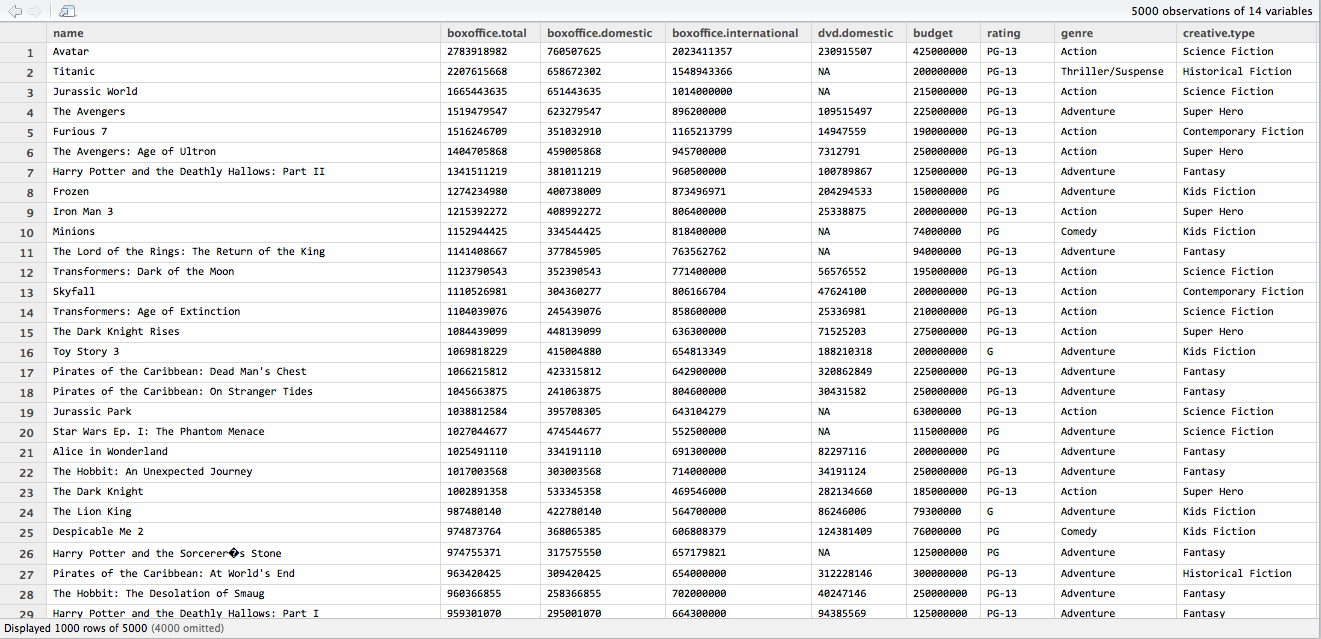
\includegraphics[width=\linewidth]{/Users/Nathaniel/Dropbox/Git/YaRrr_Book/media/moviesscreenshot.png}
\caption{Screenshot of the movies dataset.}
\label{fig:moviesscreen}
\end{figure}

Let's start by looking at the names of the dataset using the \texttt{names()} function:

\begin{knitrout}
\definecolor{shadecolor}{rgb}{0.969, 0.969, 0.969}\color{fgcolor}\begin{kframe}
\begin{alltt}
\hlkwd{names}\hlstd{(movies)}
\end{alltt}
\begin{verbatim}
##  [1] "name"                            "boxoffice.total"                
##  [3] "boxoffice.domestic"              "boxoffice.international"        
##  [5] "dvd.domestic"                    "budget"                         
##  [7] "rating"                          "genre"                          
##  [9] "creative.type"                   "time"                           
## [11] "year"                            "production.method"              
## [13] "sequel"                          "boxoffice.domestic.inflationadj"
## [15] "budget.millions"                 "boxoffice.total.millions"       
## [17] "revenue.d.budget"
\end{verbatim}
\end{kframe}
\end{knitrout}


Let's answer 5 questions with this dataset:

\subsection{Q1: What was the mean box-office total of Action movies and Adventure movies separately?}

\marginnote{In this example (and in future examples), I'm combining the \texttt{with()} and \texttt{subset()} functions. This means that I'm first telling R to use the particular subset of the data that I want, and only then do the main calculation (like the \texttt{mean}).}

% \vspace{5mm}
% \begin{minipage}{16cm}
\begin{knitrout}
\definecolor{shadecolor}{rgb}{0.969, 0.969, 0.969}\color{fgcolor}\begin{kframe}
\begin{alltt}
\hlstd{action.mean} \hlkwb{<-} \hlkwd{with}\hlstd{(}\hlkwd{subset}\hlstd{(movies, genre} \hlopt{==} \hlstr{"Action"}\hlstd{),}
                    \hlkwd{mean}\hlstd{(boxoffice.total,} \hlkwc{na.rm} \hlstd{= T))}

\hlstd{action.mean} \hlcom{# Print result}
\end{alltt}
\begin{verbatim}
## [1] 148745191
\end{verbatim}
\begin{alltt}
\hlstd{adventure.mean} \hlkwb{<-} \hlkwd{with}\hlstd{(}\hlkwd{subset}\hlstd{(movies, genre} \hlopt{==} \hlstr{"Adventure"}\hlstd{),}
                    \hlkwd{mean}\hlstd{(boxoffice.total,} \hlkwc{na.rm} \hlstd{= T))}

\hlstd{adventure.mean} \hlcom{# Print result}
\end{alltt}
\begin{verbatim}
## [1] 234682919
\end{verbatim}
\end{kframe}
\end{knitrout}
% \end{minipage}

\textbf{Answer}: The mean box office total of action movies was 149 Million. For adventure movies, the mean was  235 Million.


\subsection{Q2: Was there a difference in the production budget of Super Hero versus Science Fiction movies?}

\begin{knitrout}
\definecolor{shadecolor}{rgb}{0.969, 0.969, 0.969}\color{fgcolor}\begin{kframe}
\begin{alltt}
\hlcom{# First let's convert the budget to millions}
\hlstd{movies}\hlopt{$}\hlstd{budget.millions} \hlkwb{<-} \hlstd{movies}\hlopt{$}\hlstd{budget} \hlopt{/} \hlnum{1000000}

\hlstd{sh.budget.summary} \hlkwb{<-} \hlkwd{with}\hlstd{(}\hlkwd{subset}\hlstd{(movies, creative.type} \hlopt{==} \hlstr{"Super Hero"}\hlstd{),}
     \hlkwd{summary}\hlstd{(budget.millions))}
\hlstd{sh.budget.summary}
\end{alltt}
\begin{verbatim}
##    Min. 1st Qu.  Median    Mean 3rd Qu.    Max. 
##     0.0    60.0   120.0   117.0   152.5   275.0
\end{verbatim}
\begin{alltt}
\hlstd{sf.budget.summary} \hlkwb{<-} \hlkwd{with}\hlstd{(}\hlkwd{subset}\hlstd{(movies, creative.type} \hlopt{==} \hlstr{"Science Fiction"}\hlstd{),}
     \hlkwd{summary}\hlstd{(budget.millions))}
\hlstd{sf.budget.summary}
\end{alltt}
\begin{verbatim}
##    Min. 1st Qu.  Median    Mean 3rd Qu.    Max. 
##    0.00   10.00   38.00   55.71   80.00  425.00
\end{verbatim}
\end{kframe}
\end{knitrout}

\textbf{Answer}: Super Hero movies had higher budgets on average than Science Fiction movies. For example, the median budget of Super Hero movies was 120 Million, while median budget of Science Fiction movies was just 38.

\subsection{Q3: Were are higher percentage of R rated movies in the Action genre than the Thriller/Suspense genre?}
\marginnote{Any time you need to answer a percentage question, it's almost always a good idea to first convert the data to a logical vector, where target cases are TRUE, and then take the mean. In this example, I'm calculating the mean of the logical vector \texttt{rating == "R"}.}
\begin{knitrout}
\definecolor{shadecolor}{rgb}{0.969, 0.969, 0.969}\color{fgcolor}\begin{kframe}
\begin{alltt}
\hlstd{action.r.percentage} \hlkwb{<-} \hlkwd{with}\hlstd{(}\hlkwd{subset}\hlstd{(movies, genre} \hlopt{==} \hlstr{"Action"}\hlstd{),}
                            \hlkwd{mean}\hlstd{(rating} \hlopt{==} \hlstr{"R"}\hlstd{,} \hlkwc{na.rm} \hlstd{= T))}
\hlstd{action.r.percentage}
\end{alltt}
\begin{verbatim}
## [1] 0.4894737
\end{verbatim}
\begin{alltt}
\hlstd{thriller.r.percentage} \hlkwb{<-} \hlkwd{with}\hlstd{(}\hlkwd{subset}\hlstd{(movies, genre} \hlopt{==} \hlstr{"Thriller/Suspense"}\hlstd{),}
                              \hlkwd{mean}\hlstd{(rating} \hlopt{==} \hlstr{"R"}\hlstd{,} \hlkwc{na.rm} \hlstd{= T))}
\hlstd{thriller.r.percentage}
\end{alltt}
\begin{verbatim}
## [1] 0.6216216
\end{verbatim}
\end{kframe}
\end{knitrout}

\textbf{Answer}: Of the action movies, 49\% were rated R. Of the Thriller / Suspense movies, the percentage was 62\%

\subsection{Q4: Did movies with a running time longer than 100 minutes make more money than those with a running time less than 100 minutes??}

\begin{knitrout}
\definecolor{shadecolor}{rgb}{0.969, 0.969, 0.969}\color{fgcolor}\begin{kframe}
\begin{alltt}
\hlcom{# First let's create a new column giving boxoffice total in}
\hlcom{#  millions}

\hlstd{movies}\hlopt{$}\hlstd{boxoffice.total.millions} \hlkwb{<-} \hlstd{movies}\hlopt{$}\hlstd{boxoffice.total} \hlopt{/} \hlnum{1000000}

\hlcom{# Now we'll calculate the averages}

\hlstd{earnings.gt100} \hlkwb{<-} \hlkwd{with}\hlstd{(}\hlkwd{subset}\hlstd{(movies, time} \hlopt{>} \hlnum{100}\hlstd{),}
                       \hlkwd{mean}\hlstd{(boxoffice.total.millions))}
\hlstd{earnings.gt100}
\end{alltt}
\begin{verbatim}
## [1] 180.5893
\end{verbatim}
\begin{alltt}
\hlstd{earnings.lt100} \hlkwb{<-} \hlkwd{with}\hlstd{(}\hlkwd{subset}\hlstd{(movies, time} \hlopt{<} \hlnum{100}\hlstd{),}
                       \hlkwd{mean}\hlstd{(boxoffice.total.millions))}
\hlstd{earnings.lt100}
\end{alltt}
\begin{verbatim}
## [1] 125.5432
\end{verbatim}
\end{kframe}
\end{knitrout}

\textbf{Answer}: Longer movies tended to make more money. Movies with a running time greater than 100 minutes made 180.59 Million on average, while those with a running time less than 100 made 125.54 Million on average.

\subsection{Q5: What was the name of the movie that earned the highest box-office relative to its production budget?}


\begin{knitrout}
\definecolor{shadecolor}{rgb}{0.969, 0.969, 0.969}\color{fgcolor}\begin{kframe}
\begin{alltt}
\hlstd{movies}\hlopt{$}\hlstd{revenue.d.budget} \hlkwb{<-} \hlkwd{with}\hlstd{(movies, boxoffice.total.millions} \hlopt{/} \hlstd{budget.millions)}
\hlstd{max.val} \hlkwb{<-} \hlkwd{with}\hlstd{(}\hlkwd{subset}\hlstd{(movies, budget.millions} \hlopt{>} \hlnum{0}\hlstd{),} \hlkwd{max}\hlstd{(revenue.d.budget))}
\hlstd{max.val} \hlcom{# Print the maximum percentage increase (not necessary)}
\end{alltt}
\begin{verbatim}
## [1] 4138.333
\end{verbatim}
\begin{alltt}
\hlstd{movies}\hlopt{$}\hlstd{name[movies}\hlopt{$}\hlstd{revenue.d.budget} \hlopt{==} \hlstd{max.val]}
\end{alltt}
\begin{verbatim}
## [1] "The Blair Witch Project"
\end{verbatim}
\end{kframe}
\end{knitrout}

\marginnote{Question 5 is a bit tricky. First, I calculated a new column that divided a movie's box-office revenue by it budget called \texttt{revenue.d.budget}. Next, I calculated the maximum \texttt{revenue.d.budget} value in the dataset but \textit{only} for those movies with a budget greater than 0. Finally, I indexed the names of the movies by only looking at the rows where the \texttt{revenue.d.budget} was equal to the maximum \texttt{revenue.d.budget} value.}
\textbf{Answer}: The Blair Witch Project made 4138 times its production budget!



\section{Test your R Might!}

\begin{enumerate}

\item What was the box-office total of \texttt{"Life of Pi"}? What was its budget?

\item What was the median budget of movies made in the year 2009? What percent of these movies were sequels?

\item What percent of Science Fiction movies (look in the \texttt{creative.type} column) were rated PG-13? Of these movies, what was the median budget?

\item How many Action movies had a budget less than 150 million? Of these movies, what was the name of the movie with the highest box-office total and how much did it earn?

\item Which movie had the worst box-office total relative to its budget? What was the genre of this movie?

\end{enumerate}



%----------------------------------------------------------------------------------------
%	CHAPTER 10
%----------------------------------------------------------------------------------------

\chapter{7: Grouped aggregation with dataframes}
\label{ch:7}


Chapter Goals

\begin{enumerate}
  \item Grouped aggregation with aggregate() and dplyr
\end{enumerate}

\section{Grouped aggregation with aggregate()}

Many of the questions we might want to answer with a dataset have to do with comparisons between groups. For example, in our pirates dataset we could ask ``What is the average age of pirates from each college?" or "Do older pirates tend to have faster sword speeds?" In each of these questions, we want to know a descriptive statistic of a numeric variable (age and sword speed) as a function of one or more independent variables (college and age). By now, your R skills are good enough that you \textit{could} answer these questions already. You could use \texttt{subset()} or logical indexing to slice and dice the data set for each level of the independent variable. However, it would be a pain to have to manually create new subsets or indexes for each level of the independent variable. Thankfully, R contains many functions that will help you do this in a snap.

The first function we'll cover is \texttt{aggregate()}. The function \texttt{aggregate()} takes three arguments, a formula in the form  \texttt{y {\raise.17ex\hbox{$\scriptstyle\sim$}} x1 + x2} defining the dependent (Y) and one or more independent variables (x1, x2, ...), a function (FUN), and a dataframe (data). When you execute \texttt{aggregate(\texttt{y {\raise.17ex\hbox{$\scriptstyle\sim$}} x1 + x2 + ...}, data, FUN)}, R will apply the input function (FUN) to the dependent variable (Y) \textit{separately} for each level(s) of the independent variable(s) (x1, x2, ...). Let's see how it works:


\vspace{5mm} %5mm vertical space
\noindent
\setlength{\fboxrule}{1.5pt}
\fbox{
\parbox{\textwidth}{

\newfun{aggregate()}\index{aggregate()}

\hline

\begin{description}

  \item[\tt{formula}] \hfill \\
     A formula in the form \texttt{y {\raise.17ex\hbox{$\scriptstyle\sim$}} x1 + x2 + ...} where y is the dependent variable, and x1, x2... are the index (independent) variables. For example, \texttt{salary {\raise.17ex\hbox{$\scriptstyle\sim$}} sex + age} will aggregate a \texttt{salary} column at every unique combination of \texttt{age} and \texttt{age}
        \item[\tt{FUN}] \hfill \\
   A function that you want to apply to x at every level of the independent variables. For example, \texttt{FUN = mean} will calculate the mean for each level of the independent variables.
         \item[\tt{data}] \hfill \\
The dataset containing the variables in \texttt{formula}
        \item[\tt{...}] \hfill \\
Optional arguments passed on to FUN (like \tt{na.rm = T} to ignore NA values in x)

\end{description}

}
}
\vspace{5mm} %5mm vertical space


Let's give \texttt{aggregate()} a whirl. No...not a whirl...we'll give it a spin. Definitely a spin. We'll use the function to answer the question ``What is the average (mean) age of pirates from each college?" For this question, we'll set the value of the dependent variable Y to \texttt{age}, x1 to \texttt{college}, and FUN to \texttt{mean}

\begin{footnotesize}
\begin{knitrout}
\definecolor{shadecolor}{rgb}{0.969, 0.969, 0.969}\color{fgcolor}\begin{kframe}
\begin{alltt}
\hlkwd{aggregate}\hlstd{(}\hlkwc{formula} \hlstd{= age} \hlopt{~} \hlstd{college,}  \hlcom{# DV is cancelled, IV is carrier}
          \hlkwc{FUN} \hlstd{= mean,} \hlcom{# Calculate the mean of the DV for each IV level}
          \hlkwc{na.rm} \hlstd{= T,} \hlcom{# Ignore NA values when calculating the mean}
          \hlkwc{data} \hlstd{= pirates} \hlcom{# IV and DV are located in the Flights dataframe}
          \hlstd{)}
\end{alltt}
\begin{verbatim}
##   college      age
## 1    CCCC 24.48126
## 2   JSSFP 33.23123
\end{verbatim}
\end{kframe}
\end{knitrout}
\end{footnotesize}

As you can see, the \texttt{aggregate()} function has returned a dataframe with a column for the independent variable (\texttt{college}), and a column for the results of the function \texttt{mean} applied to each level of the independent variable. We can easily plot these data using the \texttt{barplot()} function, which plots a numeric variable as a function of a nominal variable (see margin Figure~\ref{fig:barplot})

\begin{marginfigure}
\begin{tiny}
\begin{knitrout}
\definecolor{shadecolor}{rgb}{0.969, 0.969, 0.969}\color{fgcolor}\begin{kframe}
\begin{alltt}
\hlstd{aggregated.data} \hlkwb{<-} \hlkwd{aggregate}\hlstd{(}\hlkwc{formula} \hlstd{= age} \hlopt{~} \hlstd{college,}
                             \hlkwc{FUN} \hlstd{= mean,} \hlkwc{na.rm} \hlstd{= T,} \hlkwc{data} \hlstd{= pirates)}

\hlkwd{barplot}\hlstd{(}\hlkwc{height} \hlstd{= aggregated.data}\hlopt{$}\hlstd{age,}
        \hlkwc{names.arg} \hlstd{= aggregated.data}\hlopt{$}\hlstd{college)}
\end{alltt}
\end{kframe}
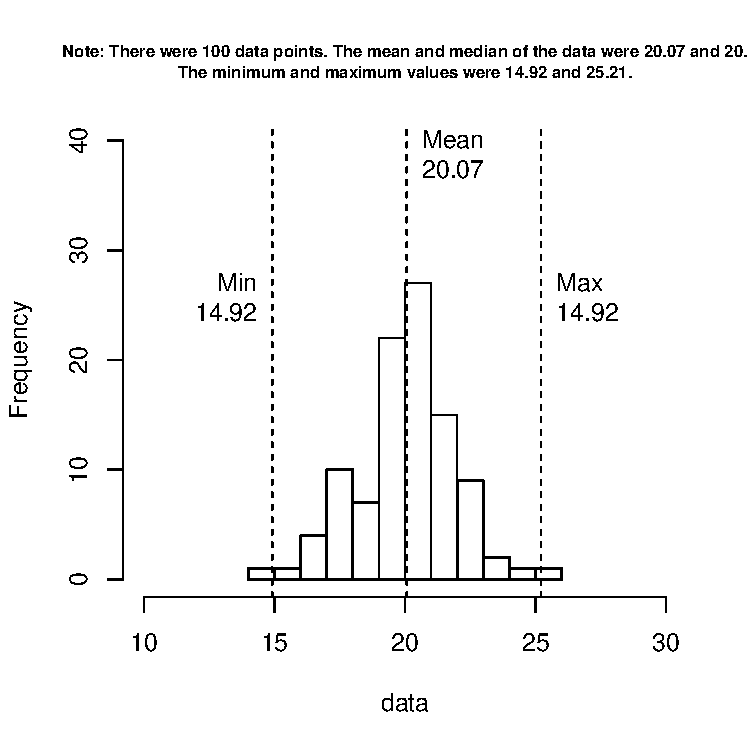
\includegraphics[width=\maxwidth]{figure/unnamed-chunk-170-1} 

\end{knitrout}
\end{tiny}
\caption{Barplot showing the mean age for each pirate college}
\label{fig:barplot}
\end{marginfigure}

You can include any function as the argument to \texttt{FUN} as long as the function takes a single numeric argument and returns a single scalar. You can also include multiple independent variables. For example, let's use \texttt{aggregate()} to now get the maximum age (i.e.; the oldest pirate) for all combinations of college and headband:

\begin{footnotesize}
\begin{knitrout}
\definecolor{shadecolor}{rgb}{0.969, 0.969, 0.969}\color{fgcolor}\begin{kframe}
\begin{alltt}
\hlcom{# Calculate median departure delay by carrier}
\hlstd{agg.data} \hlkwb{<-} \hlkwd{aggregate}\hlstd{(}
            \hlkwc{formula} \hlstd{= age} \hlopt{~} \hlstd{college} \hlopt{+} \hlstd{headband,} \hlcom{# DV is age, IV is college and headband}
            \hlkwc{FUN} \hlstd{= max,} \hlcom{# Calculate the median age}
            \hlkwc{data} \hlstd{= pirates,} \hlcom{# Columns are in the pirates dataframe}
            \hlkwc{na.rm} \hlstd{= T)} \hlcom{# Ignore NA values when calculating the median}

\hlstd{agg.data} \hlcom{# print the result!}
\end{alltt}
\begin{verbatim}
##   college headband age
## 1    CCCC       no  32
## 2   JSSFP       no  45
## 3    CCCC      yes  34
## 4   JSSFP      yes  43
\end{verbatim}
\end{kframe}
\end{knitrout}
\end{footnotesize}


While \texttt{aggregate()} is good for calculating summary statistics for a single dependent variable, it can't handle multiple dependent variables. For example, if you wanted to calculate summary statistics for multiple dependent variables (like age, sword speed, height, etc.), you'd need to execute an \texttt{aggregate()} command for each dependent variable, and then combine the results into a single dataframe. Thankfully, a recently released R package called \texttt{dplyr} makes this process very simple!

\section{Aggregation with dplyr}

The \texttt{dplyr} package is a relatively new R package that allows you to do all kinds of analyses quickly and easily. In this section, we'll go over a very brief overview of how you can use dplyr to easily do grouped aggregation. Just to be clear - you can use dplyr to do everything the \texttt{aggregate()} function does and much more! However, this will be a very brief overview and I strongly recommend you look at the help menu for dplyr for additional descriptions and examples.

Programming with dplyr looks a lot different than programming in standard R. dplyr works by combining objects (dataframes and columns in dataframes), functions (mean, median, etc.), and \textit{verbs} (special commands in \texttt{dplyr}). In between these commands is a new operator called the \textit{pipe} which looks like this: \texttt{\%>\%}. The pipe simply tells R that you want to continue executing some functions or verbs on the object you are working on. You can think about this pipe as meaning 'and then...'

\begin{marginfigure}

The pipe operator \%>\% in dplyr is used to link multiple arguments sequentially. You can think of \%>\% as meaning ``and then...''

\end{marginfigure}

To aggregate data with \texttt{dplyr}, your code will look something like the following code. In this example, assume that the original (raw) dataframe is called
\texttt{my.df}, the variable you want to collapse the data over is called \texttt{grouping.column}, and the columns you want to aggregate are called \texttt{col.a}, \texttt{col.b} and \texttt{col.c}

\begin{knitrout}
\definecolor{shadecolor}{rgb}{0.969, 0.969, 0.969}\color{fgcolor}\begin{kframe}
\begin{alltt}
\hlstd{my.df} \hlopt  \hlcom{# Specify original dataframe}
    \hlkwd{group_by}\hlstd{(grouping.column)} \hlopt \hlcom{# Grouping variable}
    \hlkwd{summarise}\hlstd{(}
      \hlkwc{a.mean} \hlstd{=} \hlkwd{mean}\hlstd{(col.a),}  \hlcom{# calculate mean of column col.a in my.df}
      \hlkwc{b.sd} \hlstd{=} \hlkwd{sd}\hlstd{(col.b),}      \hlcom{# calculate sd of column col.b in my.df}
      \hlkwc{c.max} \hlstd{=} \hlkwd{max}\hlstd{(col.c)}     \hlcom{# calculate max on column col.c in my.df, ...}
      \hlstd{)}
\end{alltt}
\end{kframe}
\end{knitrout}

Here's how you should think about the code above:

\begin{displayquote}
Start with the dataframe \texttt{my.df}. \textit{Then}, group \texttt{my.df} by the grouping variable \texttt{grouping.variable}. \textit{Then}, calculate the following summary columns in the dataset: \texttt{a.mean} should be the mean of \texttt{col.a} in my.df, \texttt{b.sd} should be the standard deviation of \texttt{col.b} in my.df, and \texttt{c.max} should be the maximum value of \texttt{col.c} in my.df.
\end{displayquote}

When you use dplyr, you write code that sounds like: "The original dataframe is XXX, now filter the dataframe to only include rows that satisfy the conditions YYY, now group the data at each level of the variable(s) ZZZ, now summarize the data and calculate summary functions XXX..."

Let's start with an example: Let's create a dataframe of aggregated data from the \texttt{pirates} dataset. I'm going to group the data according to the columns college and headband. where each row is a unique combination of college and headband. I'll then create several columns is a different summary statistic of some data across all pirates within each grouping of college and headband. Specifically, let's create 5 columns: \texttt{age.med}, The median age of pirates, \texttt{age.min}: The minimum age of pirates, \texttt{sword.time.med}: The median sword swing time of pirates, and \texttt{tchests.mean}: The average number of treasure chests found of pirates. Finally, I will calculate how many pirates were in each group using the n() function - a function specific to dplyr that counts cases.

To create this aggregated data frame, I will use the new function \textt{group\_by} and the verb \texttt{summarise}. I will assign the result to a new dataframe called \texttt{college.agg}:

\begin{footnotesize}
\begin{knitrout}
\definecolor{shadecolor}{rgb}{0.969, 0.969, 0.969}\color{fgcolor}\begin{kframe}
\begin{alltt}
\hlkwd{library}\hlstd{(dplyr)}
\hlstd{college.agg} \hlkwb{<-} \hlstd{pirates} \hlopt \hlcom{# Define dataframe, THEN...}
                \hlkwd{group_by}\hlstd{(college, headband)} \hlopt \hlcom{# Define the grouping variable, THEN...}
  \hlkwd{summarise}\hlstd{(} \hlcom{# Tell R you are going to calculate summaries}
    \hlkwc{age.med} \hlstd{=} \hlkwd{median}\hlstd{(age),} \hlcom{# Define first summary...}
    \hlkwc{age.min} \hlstd{=} \hlkwd{min}\hlstd{(age),}  \hlcom{# Define second summary...}
    \hlkwc{sword.time.med} \hlstd{=} \hlkwd{median}\hlstd{(sword.time),}
   \hlkwc{tchests.mean} \hlstd{=} \hlkwd{mean}\hlstd{(tchests),}
   \hlkwc{n} \hlstd{=} \hlkwd{n}\hlstd{()} \hlcom{# How many are in each group?}
  \hlstd{)} \hlcom{# End}

\hlstd{college.agg} \hlcom{# Print result!}
\end{alltt}
\begin{verbatim}
## Source: local data frame [4 x 7]
## Groups: college [?]
## 
##   college headband age.med age.min sword.time.med tchests.mean     n
##     (chr)    (chr)   (dbl)   (dbl)          (dbl)        (dbl) (int)
## 1    CCCC       no      25      17           4.10     6.031250    64
## 2    CCCC      yes      25      12           0.58     6.875622   603
## 3   JSSFP       no      34      29           4.90     7.676471    34
## 4   JSSFP      yes      33      25           0.58     7.949833   299
\end{verbatim}
\end{kframe}
\end{knitrout}
\end{footnotesize}

As you can see, our final object \texttt{college.agg} is the aggregated dataframe we want which aggregates all the columns we wanted for each college and headband use. Let's walk through the code

\marginnote{When you use dplyr, the output will always be an object called a \textit{local data frame}. A local dataframe is identical to a regular dataframe, except that it looks a bit nicer if you print the entire dataframe into the console. This means you don't have to use the \texttt{head()} function when looking at a local dataframe.}

\begin{itemize}
  \item First, we define the original dataframe that we are basing our summary statistics on. In this case, the original dataframe is \texttt{pirates}. We then include the pipe \texttt{\%>\%} to tell R we are still working.
  \item Second, we define the grouping variable using the \texttt{group\_by} function. This tells R to group the results at the level of college and headband. We then use the \texttt{\%>\%} pipe.
  \item Next, we call the \texttt{summarise} function, which tells R that the following functions will be summaries of the grouping variable. Because all the arguments to the \texttt{summarise} function are within the parentheses, we don't need to use a pipe.
  \item Finally, we define the summary columns in our final dataframe. For each column, we give it a name (e.g.; \texttt{age.med}), and then write the calculation as a function of the appropriate columns in the original dataframe. For example, to define \texttt{age.med}, we write \texttt{median(age)}. The new function at the end is n(), which counts the number of cases in each group.

\end{itemize}

Hopefully you can see that this \texttt{dplyr} code is \textit{much} simpler than the code we'd have to use if we wanted to create all these summary columns using \texttt{aggregate}.

\subsection{The 5 verbs in dplyr}

In the example above, we used the \texttt{dplyr} verb \texttt{summarise}. However, dplyr has other verbs that are just as useful:

\vspace{5mm} %5mm vertical space
\noindent
\setlength{\fboxrule}{1.5pt}
\fbox{
\parbox{\textwidth}{

\newfun{dplyr verbs}\index{dplyr()}

\hline

\begin{description}

\item[\tt{filter}] \hfill \\
Select a subset of rows in a dataframe. For example, filter(sex == "male") will only include data where the column sex is male. Filter works identically to the subset() function in base-R.

\item[\tt{arrange}] \hfill \\
  Reorders rows of a dataframe according to a column. For example, arrange(age) will sort the dataframe according to an age column.

  \item[\tt{select}] \hfill \\
Select specific columns of a dataframe. There are many ways to use select, for some examples, check out http://www.r-bloggers.com/the-complete-catalog-of-argument-variations-of-select-in-dplyr/.

\item[\tt{mutate}] \hfill \\
Add a column to a dataframe. For example, \texttt{mutate(bmi = weight / height)} will create a new column called bmi that divides a column weight by height

\item[\tt{summarise}] \hfill \\
 Creates summary columns as a function of columns in the original dataframe. Note: Only use after specifying \texttt{group\_by} variables.

\end{description}

}
}
\vspace{5mm} %5mm vertical space

Let's do an example where we combine multiple verbs into one chunk of code. We'll create a new dataframe called \texttt{college.favpir.agg} that gives us aggregated data at the level of the both the college the pirate went to, and their favorite pirate. However, let's add some additional data filters this time. We'll filter the data to only include pirates who are older than 30 (\texttt{age > 40)}) and who wear a headband (\texttt{headband == "yes"}):

\begin{footnotesize}
\begin{knitrout}
\definecolor{shadecolor}{rgb}{0.969, 0.969, 0.969}\color{fgcolor}\begin{kframe}
\begin{alltt}
\hlkwd{require}\hlstd{(dplyr)}
\hlstd{college.favpir.agg} \hlkwb{<-} \hlstd{pirates} \hlopt \hlcom{# First, define the original df}
            \hlkwd{filter}\hlstd{(age} \hlopt{>} \hlnum{30} \hlopt{&} \hlstd{headband} \hlopt{==} \hlstr{"yes"}\hlstd{)} \hlopt \hlcom{# Filter by age and headband}
            \hlkwd{group_by}\hlstd{(college, favorite.pirate)} \hlopt \hlcom{# Define the grouping variable}
            \hlkwd{summarise}\hlstd{(} \hlcom{#}
              \hlkwc{frequency} \hlstd{=} \hlkwd{n}\hlstd{(),} \hlcom{# How many pirates in each group?}
              \hlkwc{sword.time.med} \hlstd{=} \hlkwd{median}\hlstd{(sword.time),}  \hlcom{# Median sword speed?}
              \hlkwc{parrots.mean} \hlstd{=} \hlkwd{mean}\hlstd{(parrots)} \hlcom{# # mean parrots?}
            \hlstd{)} \hlopt
            \hlkwd{arrange}\hlstd{(frequency)} \hlcom{# Step 7}

\hlstd{college.favpir.agg} \hlcom{# Print the result!}
\end{alltt}
\begin{verbatim}
## Source: local data frame [12 x 5]
## Groups: college [2]
## 
##    college favorite.pirate frequency sword.time.med parrots.mean
##      (chr)           (chr)     (int)          (dbl)        (dbl)
## 1     CCCC      Blackbeard         1          6.360     4.000000
## 2     CCCC      Lewis Scot         2          0.285     4.500000
## 3     CCCC        Anicetus         3          0.430     5.333333
## 4     CCCC      Edward Low         3          0.560     3.333333
## 5     CCCC            Hook         4          0.300     3.250000
## 6     CCCC    Jack Sparrow         8          0.350     4.500000
## 7    JSSFP      Blackbeard        23          0.590     3.086957
## 8    JSSFP        Anicetus        25          0.570     3.280000
## 9    JSSFP            Hook        31          0.580     3.419355
## 10   JSSFP      Lewis Scot        34          0.675     3.029412
## 11   JSSFP      Edward Low        47          0.550     4.340426
## 12   JSSFP    Jack Sparrow        72          0.510     3.041667
\end{verbatim}
\end{kframe}
\end{knitrout}
\end{footnotesize}

As you can see, our result is a dataframe with 12 rows and 5 columns. Let's walk through the code line by line:

\begin{enumerate}

  \item First, we define the original dataframe as \texttt{pirates}, (\%>\% then...)
  \item Next we filter the \texttt{pirates} dataframe by only including rows where age is greater than 30 and headband is yes (\%>\% then...)
  \item We group the data according to \texttt{college} and \texttt{favorite.pirate} (\%>\% then...)
  \item We call the \texttt{summarise} verb, telling dplyr that the next commands are summary functions of \texttt{pirates}. These will be the columns in our new aggregated dataframe. (\%>\% then...)
  \item The first column in our new aggregated dataset is called \texttt{frequency} and is defined as the number of pirates in the group (the function \texttt{n()} is special to \texttt{dplyr} and simply returns the number of rows in a group)
  \item The second column is called \texttt{sword.time.med} and is the median sword time of pirates in the group
  \item The third column is called \texttt{parrots.mean} and is the mean number of parrots owned by pirates in the group.
  \item After closing the \texttt{summary()} function, we arrange the final dataframe by the new column \texttt{frequency}

\end{enumerate}


\section{Test your R might!}

\begin{enumerate}

\item Using the movies dataset, create a dataframe called \texttt{genre.agg} that shows the median budget of movies for each genre. Do this once using \texttt{aggregate()} function and once using dplyr.

\item Create a dataframe called \texttt{rating.agg} that groups the movies dataset by movie ratings and provides the following summary statistics: budget.mean, the mean movie budget -- sequel.p, the proportion of movie sequels -- and n, the number of movies with that rating.

\end{enumerate}


\section{Additional Tips}

\begin{itemize}

  \item There is an entire class of functions in R that apply functions to groups of data. One common one is \texttt{tapply(), sapply() and lapply()} which work very similarly to \texttt{aggregate()}. For example, you can calculate the average length of movies by genre with \texttt{tapply()} as follows:

\begin{knitrout}
\definecolor{shadecolor}{rgb}{0.969, 0.969, 0.969}\color{fgcolor}\begin{kframe}
\begin{alltt}
\hlkwd{with}\hlstd{(movies,} \hlkwd{tapply}\hlstd{(}\hlkwc{X} \hlstd{= time,}
                    \hlkwc{INDEX} \hlstd{= genre,}
                    \hlkwc{FUN} \hlstd{= mean,}
                    \hlkwc{na.rm} \hlstd{= T))}
\end{alltt}
\end{kframe}
\end{knitrout}

  \item We have only scratched the surface of everything you can do with \texttt{dplyr}. For more \texttt{dplyr} tips, check out https://cran.rstudio.com/web/packages/dplyr/vignettes/introduction.html

\end{itemize}





%----------------------------------------------------------------------------------------
%  CHAPTER 8
%----------------------------------------------------------------------------------------

\chapter{7: Sampling and Probability Distributions}
\label{ch:8}



\section{Sampling data from probability distributions}

\begin{marginfigure}
\begin{tiny}
\begin{knitrout}
\definecolor{shadecolor}{rgb}{0.969, 0.969, 0.969}\color{fgcolor}\begin{kframe}
\begin{alltt}
\hlcom{# Create blank plot}
\hlkwd{plot}\hlstd{(}\hlnum{1}\hlstd{,} \hlkwc{xlim} \hlstd{=} \hlkwd{c}\hlstd{(}\hlnum{0}\hlstd{,} \hlnum{100}\hlstd{),} \hlkwc{ylim} \hlstd{=} \hlkwd{c}\hlstd{(}\hlnum{0}\hlstd{,} \hlnum{100}\hlstd{),}
     \hlkwc{xlab} \hlstd{=} \hlstr{"Pirate Quality"}\hlstd{,} \hlkwc{ylab} \hlstd{=} \hlstr{""}\hlstd{,} \hlkwc{type} \hlstd{=} \hlstr{"n"}\hlstd{,}
     \hlkwc{main} \hlstd{=} \hlstr{"Two different Pirate colleges"}\hlstd{,} \hlkwc{yaxt} \hlstd{=} \hlstr{"n"}
     \hlstd{)}

\hlcom{# Set colors}
\hlkwd{require}\hlstd{(}\hlstr{"RColorBrewer"}\hlstd{)}
\hlstd{col.vec} \hlkwb{<-} \hlkwd{brewer.pal}\hlstd{(}\hlnum{10}\hlstd{,} \hlkwc{name} \hlstd{=} \hlstr{"Set3"}\hlstd{)[}\hlnum{4}\hlopt{:}\hlnum{6}\hlstd{]}

\hlcom{# Draw Samples}
\hlstd{samples.1} \hlkwb{<-} \hlkwd{runif}\hlstd{(}\hlkwc{n} \hlstd{=} \hlnum{5}\hlstd{,} \hlnum{40}\hlstd{,} \hlnum{60}\hlstd{)}
\hlstd{samples.2} \hlkwb{<-} \hlkwd{runif}\hlstd{(}\hlkwc{n} \hlstd{=} \hlnum{5}\hlstd{,} \hlnum{10}\hlstd{,} \hlnum{90}\hlstd{)}

\hlkwd{text}\hlstd{(}\hlnum{50}\hlstd{,} \hlnum{90}\hlstd{,} \hlstr{"Pirate Training Unlimited"}\hlstd{,} \hlkwc{font} \hlstd{=} \hlnum{3}\hlstd{)}

\hlkwa{for}\hlstd{(i} \hlkwa{in} \hlnum{1}\hlopt{:}\hlkwd{length}\hlstd{(samples.1)) \{}

  \hlkwd{points}\hlstd{(samples.1[i],} \hlnum{75}\hlstd{,} \hlkwc{pch} \hlstd{=} \hlnum{21}\hlstd{,} \hlkwc{bg} \hlstd{= col.vec[}\hlnum{1}\hlstd{],} \hlkwc{cex} \hlstd{=} \hlnum{3}\hlstd{)}
  \hlkwd{text}\hlstd{(samples.1[i],} \hlnum{75}\hlstd{,} \hlkwd{round}\hlstd{(samples.1[i],} \hlnum{0}\hlstd{))}

\hlstd{\}}

\hlkwd{segments}\hlstd{(}\hlnum{40}\hlstd{,} \hlnum{65}\hlstd{,} \hlnum{60}\hlstd{,} \hlnum{65}\hlstd{,} \hlkwc{col} \hlstd{= col.vec[}\hlnum{1}\hlstd{],} \hlkwc{lty} \hlstd{=} \hlnum{1}\hlstd{,} \hlkwc{lwd} \hlstd{=} \hlnum{2}\hlstd{)}

\hlkwd{text}\hlstd{(}\hlnum{50}\hlstd{,} \hlnum{40}\hlstd{,} \hlstr{"Unlimited Pirate Training"}\hlstd{,} \hlkwc{font} \hlstd{=} \hlnum{3}\hlstd{)}

\hlkwa{for}\hlstd{(i} \hlkwa{in} \hlnum{1}\hlopt{:}\hlkwd{length}\hlstd{(samples.2)) \{}

  \hlkwd{points}\hlstd{(samples.2[i],} \hlnum{25}\hlstd{,} \hlkwc{pch} \hlstd{=} \hlnum{21}\hlstd{,} \hlkwc{bg} \hlstd{= col.vec[}\hlnum{2}\hlstd{],} \hlkwc{cex} \hlstd{=} \hlnum{3}\hlstd{)}
  \hlkwd{text}\hlstd{(samples.2[i],} \hlnum{25}\hlstd{,} \hlkwd{round}\hlstd{(samples.2[i],} \hlnum{0}\hlstd{))}

\hlstd{\}}

\hlkwd{segments}\hlstd{(}\hlnum{10}\hlstd{,} \hlnum{15}\hlstd{,} \hlnum{90}\hlstd{,} \hlnum{15}\hlstd{,} \hlkwc{col} \hlstd{= col.vec[}\hlnum{2}\hlstd{],} \hlkwc{lty} \hlstd{=} \hlnum{1}\hlstd{,} \hlkwc{lwd} \hlstd{=} \hlnum{2}\hlstd{)}
\end{alltt}
\end{kframe}
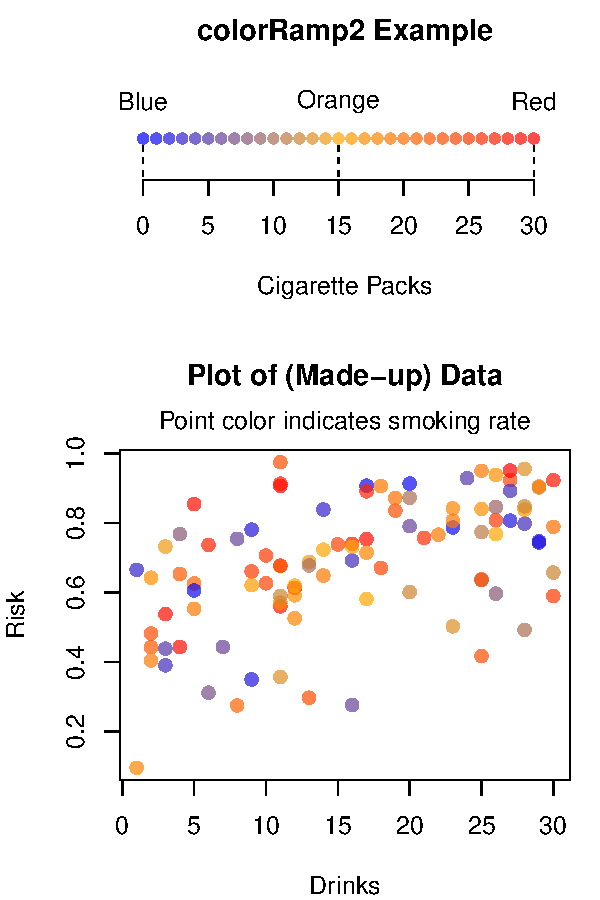
\includegraphics[width=\maxwidth]{figure/unnamed-chunk-176-1} 

\end{knitrout}
\end{tiny}
\caption{Sampling 5 potential pirates from two different pirate colleges. Pirate Training Unlimited (PTU) consistently produces average pirates (with scores between 40 and 60), while Unlimited Pirate Training (UPT), produces a wide range of pirates from 0 to 100.}
\label{fig:piratecollege}
\end{marginfigure}


By now you know how to generate sequences of numbers with the functions :, \texttt{seq()}, and \texttt{rep()}. However, these functions don't generate very interesting data. Instead, we can use R to generate randomly sampled data from specified \textit{probability distributions}. A probability distribution is simply an equation -- also called a likelihood function -- that indicates how likely certain numerical values are to be drawn.


For example, imagine you need to hire a new group of pirates for your crew. You have the option of hiring people form one of two different pirate training colleges that produce pirates of varying quality. One college ``Pirate Training Unlimited" might tend to pirates that are generally ok - never great but never terrible. While another college ``Unlimited Pirate Training" might produce pirates with a wide variety of quality, from very low to very high. In Figure~\ref{fig:piratecollege} I plotted 5 example pirates from each college, where each pirate is shown as a ball with a number written on it. As you can see, pirates from PTU all tend to be clustered between 40 and 60 (not terrible but not great), while pirates from UPT are all over the map, from 0 to 100. We can use probability distributions (in this case, the uniform distribution) to mathematically define how likely any possible value is to be drawn at random from a distribution.

%\marginnote{Mathematically, a probability distribution must satisfy two criteria: 1) All likelihoods must be positive, 2) The sum (or integral) of all likelihoods must equal 1.}

In the next section we'll go over some of the most commonly used sampling distributions: the Normal and Uniform distributions.

\pagebreak
\subsection{The Normal (Gaussian) distribution}

\begin{marginfigure}
\begin{tiny}
\begin{knitrout}
\definecolor{shadecolor}{rgb}{0.969, 0.969, 0.969}\color{fgcolor}\begin{kframe}
\begin{alltt}
\hlkwd{require}\hlstd{(}\hlstr{"RColorBrewer"}\hlstd{)}

\hlcom{# Create blank plot}
\hlkwd{plot}\hlstd{(}\hlnum{1}\hlstd{,} \hlkwc{xlim} \hlstd{=} \hlkwd{c}\hlstd{(}\hlopt{-}\hlnum{5}\hlstd{,} \hlnum{5}\hlstd{),} \hlkwc{ylim} \hlstd{=} \hlkwd{c}\hlstd{(}\hlnum{0}\hlstd{,} \hlnum{1}\hlstd{),}
     \hlkwc{xlab} \hlstd{=} \hlstr{"x"}\hlstd{,} \hlkwc{ylab} \hlstd{=} \hlstr{"dnorm(x)"}\hlstd{,} \hlkwc{type} \hlstd{=} \hlstr{"n"}\hlstd{,}
     \hlkwc{main} \hlstd{=} \hlstr{"Three Normal Distributions"}
     \hlstd{)}

\hlcom{# Set up design matrix for loop}
\hlstd{design.matrix} \hlkwb{<-} \hlkwd{data.frame}\hlstd{(}\hlstr{"mean"} \hlstd{=} \hlkwd{c}\hlstd{(}\hlnum{0}\hlstd{,} \hlopt{-}\hlnum{2}\hlstd{,} \hlnum{1}\hlstd{),}
                            \hlstr{"sd"} \hlstd{=} \hlkwd{c}\hlstd{(}\hlnum{1}\hlstd{,} \hlnum{.5}\hlstd{,} \hlnum{2}\hlstd{)}
                            \hlstd{)}
\hlcom{# Set colors}
\hlstd{col.vec} \hlkwb{<-} \hlkwd{brewer.pal}\hlstd{(}\hlnum{10}\hlstd{,} \hlkwc{name} \hlstd{=} \hlstr{"Set3"}\hlstd{)[}\hlnum{4}\hlopt{:}\hlnum{6}\hlstd{]}

\hlcom{# Start loop over distributions}
\hlkwa{for} \hlstd{(i} \hlkwa{in} \hlnum{1}\hlopt{:}\hlkwd{nrow}\hlstd{(design.matrix)) \{}

\hlstd{mean.i} \hlkwb{<-} \hlstd{design.matrix}\hlopt{$}\hlstd{mean[i]}
\hlstd{sd.i} \hlkwb{<-} \hlstd{design.matrix}\hlopt{$}\hlstd{sd[i]}

\hlstd{fun} \hlkwb{<-} \hlkwa{function}\hlstd{(}\hlkwc{x}\hlstd{) \{}
  \hlkwd{dnorm}\hlstd{(x,} \hlkwc{mean} \hlstd{= mean.i,} \hlkwc{sd} \hlstd{= sd.i)\}}

\hlkwd{curve}\hlstd{(}\hlkwc{expr} \hlstd{= fun,}
      \hlkwc{from} \hlstd{=} \hlopt{-}\hlnum{5}\hlstd{,}\hlkwc{to} \hlstd{=} \hlnum{5}\hlstd{,}
      \hlkwc{xlab} \hlstd{=} \hlstr{"x"}\hlstd{,} \hlkwc{lwd} \hlstd{=} \hlnum{3}\hlstd{,}
      \hlkwc{add} \hlstd{= T,} \hlkwc{col} \hlstd{= col.vec[i])}

\hlstd{samples} \hlkwb{<-} \hlkwd{rnorm}\hlstd{(}\hlkwc{n} \hlstd{=} \hlnum{10}\hlstd{,} \hlkwc{mean} \hlstd{= mean.i,} \hlkwc{sd} \hlstd{= sd.i)}

\hlkwd{segments}\hlstd{(}\hlkwc{x0} \hlstd{= samples,} \hlkwc{y0} \hlstd{=} \hlkwd{rep}\hlstd{(}\hlnum{0}\hlstd{,} \hlnum{10}\hlstd{),}
         \hlkwc{x1} \hlstd{= samples,} \hlkwc{y1} \hlstd{=} \hlkwd{fun}\hlstd{(samples),}
         \hlkwc{col} \hlstd{= col.vec[i],} \hlkwc{lwd} \hlstd{=} \hlnum{1}\hlstd{,} \hlkwc{lty} \hlstd{=} \hlnum{2}
         \hlstd{)}
\hlstd{\}}

\hlstd{legend.fun} \hlkwb{<-} \hlkwa{function}\hlstd{(}\hlkwc{i}\hlstd{) \{}
  \hlkwd{paste}\hlstd{(}\hlstr{"mean = "}\hlstd{, design.matrix}\hlopt{$}\hlstd{mean[i],}
        \hlstr{", sd = "}\hlstd{, design.matrix}\hlopt{$}\hlstd{sd[i],} \hlkwc{sep} \hlstd{=} \hlstr{""}\hlstd{)\}}

\hlkwd{legend}\hlstd{(}\hlstr{"topright"}\hlstd{,}
       \hlkwc{legend} \hlstd{=} \hlkwd{c}\hlstd{(}\hlkwd{legend.fun}\hlstd{(}\hlnum{1}\hlstd{),}
                  \hlkwd{legend.fun}\hlstd{(}\hlnum{2}\hlstd{),}
                  \hlkwd{legend.fun}\hlstd{(}\hlnum{3}\hlstd{)}
                  \hlstd{),}
       \hlkwc{lwd} \hlstd{=} \hlkwd{rep}\hlstd{(}\hlnum{3}\hlstd{,} \hlnum{3}\hlstd{),}
       \hlkwc{col} \hlstd{= col.vec[}\hlnum{1}\hlopt{:}\hlnum{3}\hlstd{]}
       \hlstd{)}
\end{alltt}
\end{kframe}
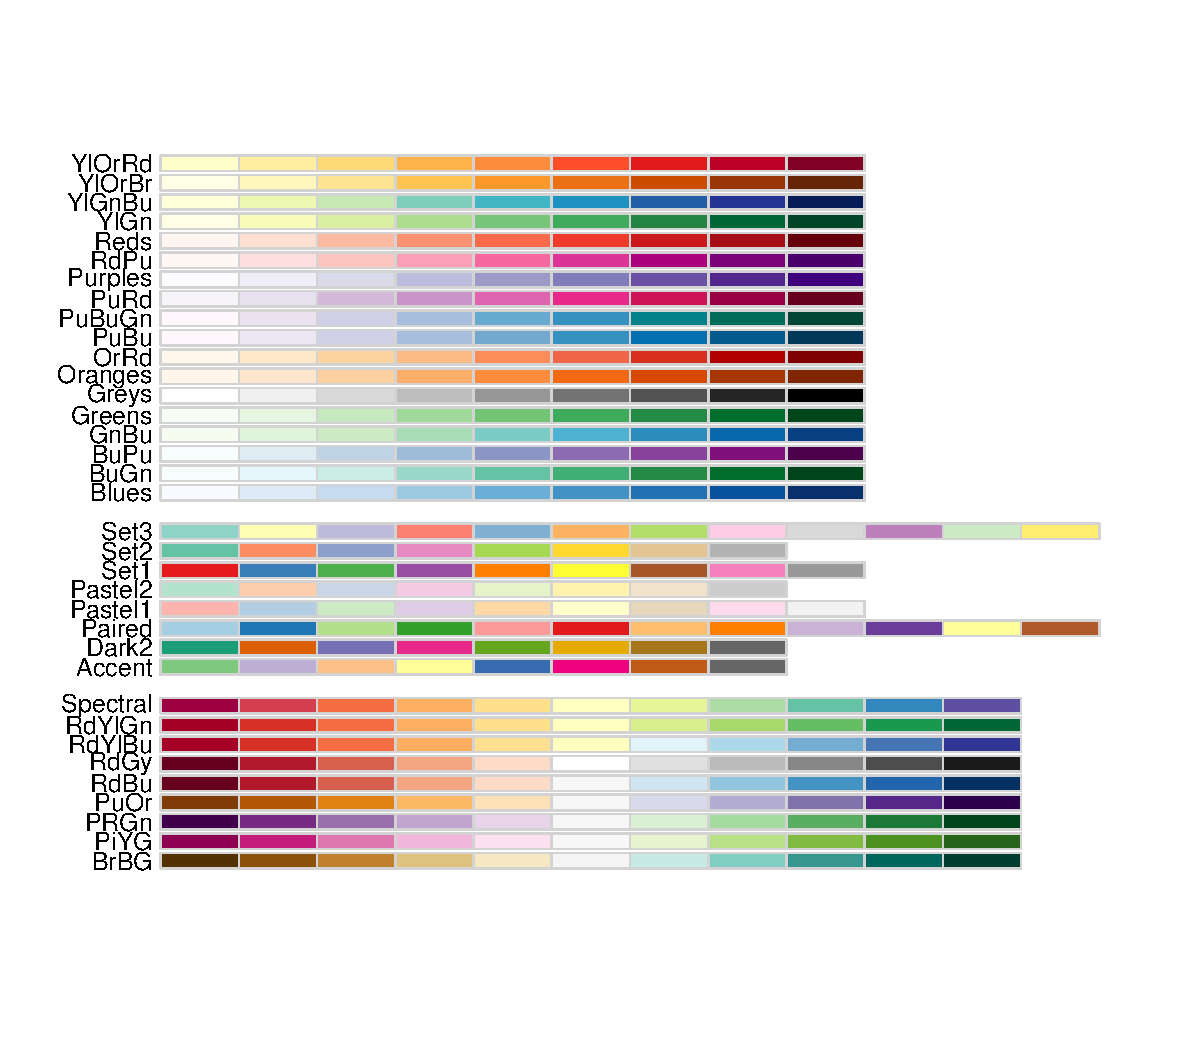
\includegraphics[width=\maxwidth]{figure/unnamed-chunk-177-1} 

\end{knitrout}
\caption{Three different normal distributions with different means and standard deviations.}
\label{fig:normaldist}
\end{tiny}
\end{marginfigure}
Let's start with the most famous distribution in statistics: the Normal (or if you want to sound pretentious, the Gaussian) distribution. The Normal distribution is bell-shaped, and has two parameters: a mean and a standard deviation. See the margin figure~\ref{fig:normaldist} for plots of three different Normal distributions with different means and standard deviations.



To generate samples from a normal distribution in R, we use the function \texttt{rnorm()} this function has three arguments:




\vspace{5mm} %5mm vertical space
\noindent
\setlength{\fboxrule}{1.5pt}
\fbox{
\parbox{\textwidth}{

\newfun{rnorm()}\index{rnorm()}

\hline

\begin{description}

\item[\tt{n}] \hfill \\
    The number of observations
\item[\tt{mean}] \hfill \\
    The mean of the Normal distribution from which samples are drawn (not the sample mean!!)
\item[\tt{sd}] \hfill \\
  The standard deviation of the Normal distribution from which samples are drawn

\end{description}

}
}
\vspace{5mm} %5mm vertical space


For example, let's draw 5 samples (\texttt{n = 5}) from a normal distribution with mean 0 (\texttt{mean = 0}) and standard deviation 1 (\texttt{sd = 1})

\begin{knitrout}
\definecolor{shadecolor}{rgb}{0.969, 0.969, 0.969}\color{fgcolor}\begin{kframe}
\begin{alltt}
\hlkwd{rnorm}\hlstd{(}\hlkwc{n} \hlstd{=} \hlnum{5}\hlstd{,} \hlkwc{mean} \hlstd{=} \hlnum{0}\hlstd{,} \hlkwc{sd} \hlstd{=} \hlnum{1}\hlstd{)}
\end{alltt}
\begin{verbatim}
## [1] 1.6184811 0.6021107 0.7290129 1.6754286 0.6640214
\end{verbatim}
\end{kframe}
\end{knitrout}

This code returns a vector of 5 values, where each value is a new random sample drawn from a Normal distribution with mean = 0 and standard deviation = 1.

Because the sampling is done randomly, you'll get different values each time you run the \texttt{rnorm()} (or any other random sampling) function. To see this, let's create two different sets of samples from a normal distribution with mean 10 and standard deviation 5 and see how they compare:

\begin{knitrout}
\definecolor{shadecolor}{rgb}{0.969, 0.969, 0.969}\color{fgcolor}\begin{kframe}
\begin{alltt}
\hlkwd{rnorm}\hlstd{(}\hlnum{5}\hlstd{,} \hlkwc{mean} \hlstd{=} \hlnum{10}\hlstd{,} \hlkwc{sd} \hlstd{=} \hlnum{5}\hlstd{)}
\end{alltt}
\begin{verbatim}
## [1]  9.109339 10.427758  9.553366  6.413901 10.697239
\end{verbatim}
\begin{alltt}
\hlkwd{rnorm}\hlstd{(}\hlnum{5}\hlstd{,} \hlkwc{mean} \hlstd{=} \hlnum{10}\hlstd{,} \hlkwc{sd} \hlstd{=} \hlnum{5}\hlstd{)}
\end{alltt}
\begin{verbatim}
## [1]  8.024336 14.333532  4.704237  4.201031 13.658394
\end{verbatim}
\end{kframe}
\end{knitrout}


As you can see, even though I used the exact same code to generate the vectors \texttt{a} and \texttt{b}, the numbers in each sample are different. That's because the samples are each drawn randomly and independently from the normal distribution. To visualize the sampling process, run the code in the margin Figure~\ref{fig:normaldist} on your machine several times. You should see the sampling lines dance around the distribution.

\subsection{The Uniform distribution}

Next, let's move on to the \textit{uniform} distribution. The uniform distribution gives equal probability to all values between the minimum and maximum values.

\begin{marginfigure}
\begin{tiny}
\begin{knitrout}
\definecolor{shadecolor}{rgb}{0.969, 0.969, 0.969}\color{fgcolor}\begin{kframe}
\begin{alltt}
\hlcom{# uniform distribution}
\hlkwd{curve}\hlstd{(dunif,}
      \hlkwc{from} \hlstd{=} \hlnum{0}\hlstd{,} \hlkwc{to} \hlstd{=} \hlnum{1}\hlstd{,}
      \hlkwc{xlim} \hlstd{=} \hlkwd{c}\hlstd{(}\hlopt{-}\hlnum{.5}\hlstd{,} \hlnum{1.5}\hlstd{),}
      \hlkwc{xlab} \hlstd{=} \hlstr{"x"}\hlstd{,}
      \hlkwc{lwd} \hlstd{=} \hlnum{2}\hlstd{,}
      \hlkwc{main} \hlstd{=} \hlstr{"Uniform\textbackslash{}nmin = 0, max = 1"}\hlstd{)}
\end{alltt}
\end{kframe}
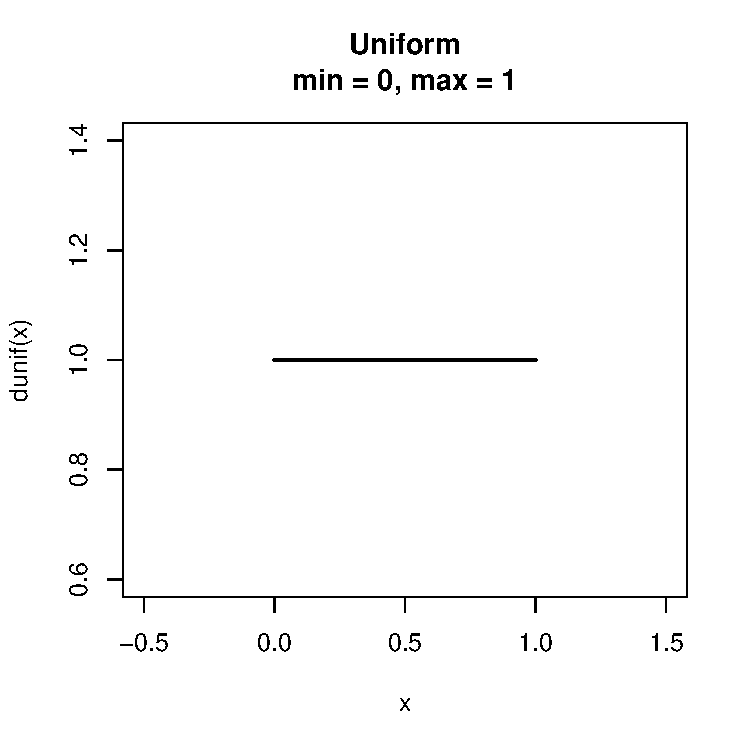
\includegraphics[width=\maxwidth]{figure/unnamed-chunk-180-1} 

\end{knitrout}
\caption{The Uniform distribution - known colloquially as the Anthony Davis distribution.}
\label{fig:unif_dist}
\end{tiny}
\end{marginfigure}


To generate samples from a uniform distribution, we use the function \texttt{runif()}, the function has 3 arguments:

\vspace{5mm} %5mm vertical space
\noindent
\setlength{\fboxrule}{1.5pt}
\fbox{
\parbox{\textwidth}{

\newfun{runif()}\index{runif()}

\hline

\begin{description}

\item[\tt{n}] \hfill \\
    The number of observations (i.e.; samples)
\item[\tt{min}] \hfill \\
    The lower bound of the Uniform distribution from which samples are drawn
\item[\tt{max}] \hfill \\
    The upper bound of the Uniform distribution from which samples are drawn
\end{description}

}
}
\vspace{5mm} %5mm vertical space

Let's draw 5 samples from two uniform distributions, one with bounds at 0 and 1, and one with bounds at -100 and 100:

\begin{footnotesize}
\begin{knitrout}
\definecolor{shadecolor}{rgb}{0.969, 0.969, 0.969}\color{fgcolor}\begin{kframe}
\begin{alltt}
\hlkwd{runif}\hlstd{(}\hlnum{5}\hlstd{,} \hlkwc{min} \hlstd{=} \hlnum{0}\hlstd{,} \hlkwc{max} \hlstd{=} \hlnum{1}\hlstd{)} \hlcom{# 5 samples from U[0, 1]}
\end{alltt}
\begin{verbatim}
## [1] 0.64137201 0.57755064 0.96007265 0.05210931 0.08823298
\end{verbatim}
\begin{alltt}
\hlkwd{runif}\hlstd{(}\hlnum{5}\hlstd{,} \hlkwc{min} \hlstd{=} \hlopt{-}\hlnum{100}\hlstd{,} \hlkwc{max} \hlstd{=} \hlnum{100}\hlstd{)} \hlcom{# 5 samples from U[-100, 100]}
\end{alltt}
\begin{verbatim}
## [1]  98.68427  26.83085 -24.17919  85.17760 -64.09378
\end{verbatim}
\end{kframe}
\end{knitrout}
\end{footnotesize}

\subsection{Sampling from a set of values: sample()}

The next function we'll use is \textbf{sample()}. The sample function works a bit differently from \texttt{runif()} and \texttt{rnorm()} because it allows to you to define which values you want to sample and the probability associated with each value. For example, if you want to simulate the flip of a fair coin, you can tell the sample function to draw the value "Heads" with probability .50, and the value "Tails" with probability .50.


\vspace{5mm} %5mm vertical space
\noindent
\setlength{\fboxrule}{1.5pt}
\fbox{
\parbox{\textwidth}{

\newfun{sample()}\index{sample()}

\hline

\begin{description}

\item[\tt{x}] \hfill \\
    A vector of outcomes you want to sample from. For example, to simulate coin flips, you'd enter \texttt{x = c("Heads", "Tails")}
\item[\tt{size}] \hfill \\
    The number of samples you want to draw.
\item[\tt{replace}] \hfill \\
    Should sampling be done with replacement? If T, then each individual sample will be replaced in the data vector. If F, then the same outcome will never be drawn more than once. Think about replacement like drawing different balls from a bag. Sampling with replacement (\texttt{replace = T}) means that each time you draw a ball, you return the ball back into the bag before drawing another ball. Sampling without replacement (\texttt{replace = F}) means that after you draw a ball, you remove that ball from the bag before drawing again.
\item[\tt{prob}] \hfill \\
    A vector of probabilities of the same length as \texttt{x} indicating how likely each outcome in "x" is. For example, to sample equally from two outcomes, you'd enter \texttt{prob = c(.5, .5)}. The first value corresponds to the first value of x and the second corresponds to the second value (etc.). The vector of probabilities you give as an argument should add up to one. However, if they don't, R will just rescale them so that they will sum to 1.

\end{description}

}
}
\vspace{5mm} %5mm vertical space


As a simple example, let's simulate 10 flips of a fair coin, were the probably of getting either a Head or Tail is .50:

\begin{footnotesize}
\begin{knitrout}
\definecolor{shadecolor}{rgb}{0.969, 0.969, 0.969}\color{fgcolor}\begin{kframe}
\begin{alltt}
\hlkwd{sample}\hlstd{(}\hlkwc{x} \hlstd{=} \hlkwd{c}\hlstd{(}\hlstr{"Heads"}\hlstd{,} \hlstr{"Tails"}\hlstd{),} \hlcom{# The values you want to sample from}
       \hlkwc{size} \hlstd{=} \hlnum{10}\hlstd{,}  \hlcom{# The number of samples}
       \hlkwc{prob} \hlstd{=} \hlkwd{c}\hlstd{(}\hlnum{.5}\hlstd{,} \hlnum{.5}\hlstd{),} \hlcom{# The probability of each value}
       \hlkwc{replace} \hlstd{= T} \hlcom{# Sampling with replacement}
       \hlstd{)}
\end{alltt}
\begin{verbatim}
##  [1] "Heads" "Tails" "Tails" "Heads" "Tails" "Tails" "Heads" "Tails"
##  [9] "Heads" "Heads"
\end{verbatim}
\end{kframe}
\end{knitrout}
\end{footnotesize}

As you can see, our function returned a vector of 10 values corresponding to our sample size of 10. Keep in mind that, just like using \texttt{rnorm()} and \texttt{runif()}, the \texttt{sample()} function can give you different outcomes every time you run it.


\begin{marginfigure}
\begin{tiny}
\begin{knitrout}
\definecolor{shadecolor}{rgb}{0.969, 0.969, 0.969}\color{fgcolor}\begin{kframe}
\begin{alltt}
\hlkwd{par}\hlstd{(}\hlkwc{mar} \hlstd{=} \hlkwd{c}\hlstd{(}\hlnum{3}\hlstd{,} \hlnum{3}\hlstd{,} \hlnum{3}\hlstd{,} \hlnum{3}\hlstd{))}
\hlkwd{plot}\hlstd{(}\hlnum{1}\hlstd{,} \hlkwc{xlim} \hlstd{=} \hlkwd{c}\hlstd{(}\hlnum{0}\hlstd{,} \hlnum{1}\hlstd{),} \hlkwc{ylim} \hlstd{=} \hlkwd{c}\hlstd{(}\hlnum{0}\hlstd{,} \hlnum{1}\hlstd{),}
     \hlkwc{xlab} \hlstd{=} \hlstr{""}\hlstd{,} \hlkwc{ylab} \hlstd{=} \hlstr{""}\hlstd{,} \hlkwc{xaxt} \hlstd{=} \hlstr{"n"}\hlstd{,}
     \hlkwc{yaxt} \hlstd{=} \hlstr{"n"}\hlstd{,} \hlkwc{type} \hlstd{=} \hlstr{"n"}\hlstd{,}
     \hlkwc{main} \hlstd{=} \hlstr{"Chest of 20 Gold, 30 Silver,\textbackslash{}nand 50 Bronze Coins"}\hlstd{)}

\hlkwd{points}\hlstd{(}\hlkwd{runif}\hlstd{(}\hlnum{100}\hlstd{,} \hlnum{.1}\hlstd{,} \hlnum{.9}\hlstd{),}
       \hlkwd{runif}\hlstd{(}\hlnum{100}\hlstd{,} \hlnum{.1}\hlstd{,} \hlnum{.9}\hlstd{),}
       \hlkwc{pch} \hlstd{=} \hlnum{21}\hlstd{,} \hlkwc{cex} \hlstd{=} \hlnum{3}\hlstd{,}
       \hlkwc{bg} \hlstd{=} \hlkwd{c}\hlstd{(}\hlkwd{rep}\hlstd{(}\hlstr{"gold"}\hlstd{,} \hlnum{20}\hlstd{),}
              \hlkwd{rep}\hlstd{(}\hlstr{"gray94"}\hlstd{,} \hlnum{30}\hlstd{),}
              \hlkwd{rep}\hlstd{(}\hlstr{"chocolate"}\hlstd{,} \hlnum{50}\hlstd{))}
       \hlstd{)}
\end{alltt}
\end{kframe}
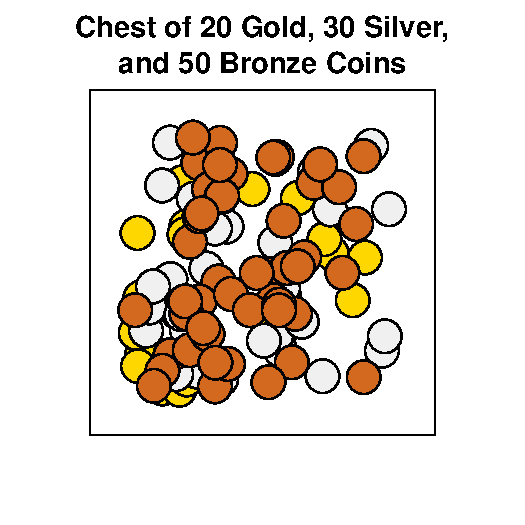
\includegraphics[width=\maxwidth]{figure/unnamed-chunk-183-1} 

\end{knitrout}
\end{tiny}
\end{marginfigure}

\subsection{Drawing coins from a treasure chest}

Now, let's sample drawing coins from a treasure chest Let's say the chest has 100 coins: 20 gold, 30 silver, and 50 bronze. Let's draw 10 random coins from this chest. Because we remove coins when we draw them, we'll set \texttt{replace = F}.

\begin{knitrout}
\definecolor{shadecolor}{rgb}{0.969, 0.969, 0.969}\color{fgcolor}\begin{kframe}
\begin{alltt}
\hlcom{# Create chest with the 100 coins}

\hlstd{chest} \hlkwb{<-} \hlkwd{c}\hlstd{(}\hlkwd{rep}\hlstd{(}\hlstr{"gold"}\hlstd{,} \hlnum{20}\hlstd{),}
         \hlkwd{rep}\hlstd{(}\hlstr{"silver"}\hlstd{,} \hlnum{30}\hlstd{),}
         \hlkwd{rep}\hlstd{(}\hlstr{"bronze"}\hlstd{,} \hlnum{50}\hlstd{)}
         \hlstd{)}

\hlcom{# Draw 10 coins from the chest without replacement}

\hlkwd{sample}\hlstd{(}\hlkwc{x} \hlstd{= chest,}
       \hlkwc{size} \hlstd{=} \hlnum{10}\hlstd{,}
       \hlkwc{prob} \hlstd{=} \hlkwd{rep}\hlstd{(}\hlnum{1} \hlopt{/} \hlnum{100}\hlstd{,} \hlkwc{times} \hlstd{=} \hlnum{100}\hlstd{),}
       \hlkwc{replace} \hlstd{= F}
       \hlstd{)}
\end{alltt}
\begin{verbatim}
##  [1] "bronze" "gold"   "bronze" "bronze" "bronze" "gold"   "bronze"
##  [8] "bronze" "bronze" "bronze"
\end{verbatim}
\end{kframe}
\end{knitrout}

The output of the \texttt{sample()} function above is a vector of 10 strings indicating the type of coin we drew on each sample. The order of these strings matter: the first one is the first coin we drew, and the last one is the 10th coin we drew. And like any random sampling function, this code will likely give you different results every time you run it! See how long it takes you to get 10 gold coins...

\subsection{Simulating Pinder Outcomes}

Let's simulate some Pinder outcomes. For those who don't know, Pinder is an app that allows Pirates to view profiles of potential dates. For each potential date, you can see their picture and either "like" them by swiping right, or "dislike" them by swiping left. If a pirate that you "liked" also "likes" you, then you've had a successful match and will be able to start chatting. let's say you "swipe right" on 20 Pinder profiles and the probability you get a match is 20\%. We can simulate this using the sample function

\begin{marginfigure}
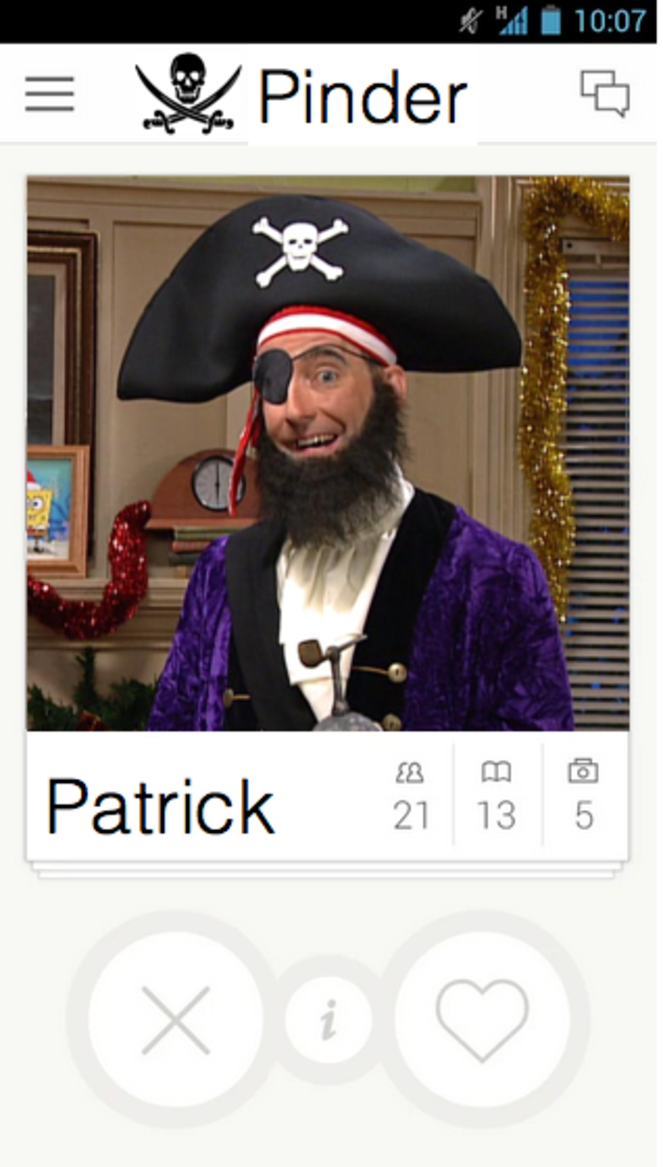
\includegraphics[width=\linewidth]{/Users/Nathaniel/Dropbox/Git/YaRrr_Book/media/pinder.pdf}
\caption{A typical Pinder profile.}
\label{fig:pinder}
\end{marginfigure}

\begin{footnotesize}
\begin{knitrout}
\definecolor{shadecolor}{rgb}{0.969, 0.969, 0.969}\color{fgcolor}\begin{kframe}
\begin{alltt}
\hlkwd{sample}\hlstd{(}\hlkwc{x} \hlstd{=} \hlkwd{c}\hlstd{(}\hlstr{"Match!!!"}\hlstd{,} \hlstr{"No Match"}\hlstd{),}
       \hlkwc{size} \hlstd{=} \hlnum{20}\hlstd{,}
       \hlkwc{replace} \hlstd{= T,} \hlcom{# Replace each sample back to the set}
       \hlkwc{prob} \hlstd{=} \hlkwd{c}\hlstd{(}\hlnum{.2}\hlstd{,} \hlnum{.8}\hlstd{)}  \hlcom{# Probability of Match! is .2, and No Match :( is .8)}
       \hlstd{)}
\end{alltt}
\begin{verbatim}
##  [1] "No Match" "No Match" "No Match" "Match!!!" "No Match" "No Match"
##  [7] "No Match" "No Match" "No Match" "Match!!!" "No Match" "No Match"
## [13] "No Match" "Match!!!" "No Match" "No Match" "No Match" "Match!!!"
## [19] "No Match" "Match!!!"
\end{verbatim}
\end{kframe}
\end{knitrout}
\end{footnotesize}

The output of this function is a simulated response from 10 pirates that you liked.

%In the example above I set \texttt{replace = T}. If I didn't do this, then on the third sample R would run out of objects to draw from. However, there are cases where we would not want sampling with replacement: for example, when deciding where to go clubbing in Berlin...

%' \subsection{Where should I go clubbing in Berlin...?}
%'
%'
%' \begin{marginfigure}
%' \begin{tiny}
%' <<fig.width = 4, fig.height = 4>>=
%' par(mar = c(4, 4, 4, 4))
%'
%' plot(1, xlim = c(0, 1), ylim = c(0, 1),
%'      xlab = "", ylab = "", xaxt = "n",
%'      yaxt = "n", type = "n", main = "Bag of clubs")
%'
%' x.vals <- runif(5, .1, .9)
%' y.vals <- runif(5, .1, .7)
%' clubs <- c("Berghain", "Club der\nVisionare",
%'              "Goldengate", "Watergate", "Keller")
%' for (i in 1:5) {
%'
%' points(x.vals[i],
%'        y.vals[i],
%'        pch = 21, cex = 13, bg = "white", lwd = 2
%'        )
%'
%'
%' text(x.vals[i], y.vals[i],
%'      labels = clubs[i], cex = .8)
%'   }
%' @
%' \end{tiny}
%' \end{marginfigure}
%'
%' Let's say you planning a weekend of clubbing in Berlin and need to decide on just 2 out of 5 clubs to visit. Since we don't want to visit the same club twice, we'll set \texttt{replace = F}. Additionally, because we want each of the clubs to be equally likely to be selected, we'll set the \texttt{prob} argument as a vector of five 1/5 values.
%'
%' \begin{footnotesize}
%' <<>>=
%' clubs <- sample(x = c("Berghain", "Club der Visionare",
%'              "Goldengate", "Watergate", "Keller"),
%'        size = 2,
%'        replace = F,
%'        prob = c(1/5, 1/5, 1/5, 1/5, 1/5) # Set the probability of each to 1/5
%'        )
%' clubs
%' @
%' \end{footnotesize}
%'
%' Looks like R has selected clubs[1] and clubs[2]. Let's see if we even make it to clubs[2]...







\section{A worked example: A quick test of the law of large numbers}

According to the law of large numbers, the larger our sample size, the closer our sample mean should be to the population mean. In other words, the more data (samples) you have, the more accurate your estimate should be. Let's test this by drawing either a small (N = 10) or a large (N = 1,000,000) number of observations from a Normal distribution with mean = 100 and sd = 20:

\marginnote{Tip: You can easily write large powers of 10 by using the notation \texttt{1eN}, where N is the power of 10. For example: \texttt{1e6} is the same as 1,000,000}

\begin{footnotesize}
\begin{knitrout}
\definecolor{shadecolor}{rgb}{0.969, 0.969, 0.969}\color{fgcolor}\begin{kframe}
\begin{alltt}
\hlstd{small} \hlkwb{<-} \hlkwd{rnorm}\hlstd{(}\hlnum{10}\hlstd{,} \hlkwc{mean} \hlstd{=} \hlnum{100}\hlstd{,} \hlkwc{sd} \hlstd{=} \hlnum{20}\hlstd{)} \hlcom{# 10 observations}
\hlstd{large} \hlkwb{<-} \hlkwd{rnorm}\hlstd{(}\hlnum{1e6}\hlstd{,} \hlkwc{mean} \hlstd{=} \hlnum{100}\hlstd{,} \hlkwc{sd} \hlstd{=} \hlnum{20}\hlstd{)} \hlcom{# One million observations}
\end{alltt}
\end{kframe}
\end{knitrout}
\end{footnotesize}

If our test worked, then the difference for the small sample should be larger than the large sample. Let's test this by calculating the mean of each sample and see how close they are to the true population mean of 100:

\begin{footnotesize}
\begin{knitrout}
\definecolor{shadecolor}{rgb}{0.969, 0.969, 0.969}\color{fgcolor}\begin{kframe}
\begin{alltt}
\hlkwd{mean}\hlstd{(small)} \hlcom{# What is the mean of the small sample?}
\end{alltt}
\begin{verbatim}
## [1] 103.6144
\end{verbatim}
\begin{alltt}
\hlkwd{mean}\hlstd{(large)} \hlcom{# What is the mean of the large sample?}
\end{alltt}
\begin{verbatim}
## [1] 99.98045
\end{verbatim}
\begin{alltt}
\hlkwd{mean}\hlstd{(small)} \hlopt{-} \hlnum{100} \hlcom{# How far is the mean of Small from 100?}
\end{alltt}
\begin{verbatim}
## [1] 3.614376
\end{verbatim}
\begin{alltt}
\hlkwd{mean}\hlstd{(large)} \hlopt{-} \hlnum{100} \hlcom{# How far is the mean of Large from 100?}
\end{alltt}
\begin{verbatim}
## [1] -0.01954734
\end{verbatim}
\end{kframe}
\end{knitrout}
\end{footnotesize}

Looks like the law of large numbers holds up!


\section{Test your R might!}

\begin{enumerate}

\item Create a vector \texttt{samp1} with 100 values drawn from a Normal distribution with a mean of 100 and a standard deviation of 20. What is the mean and median of the samples? What percent of the samples are greater than 100?

\item Create a vector called \texttt{samp2} with 50 values drawn from a Uniform distribution with a minimum of -100 and a maximum of +100. What is the What is the mean and median of the samples? What percent of the samples are greater than 50?


\begin{marginfigure}
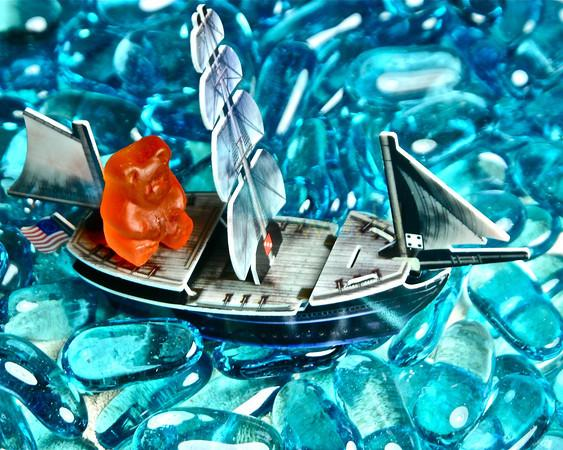
\includegraphics[width=\linewidth]{/Users/Nathaniel/Dropbox/Git/YaRrr_Book/media/gummybear.jpg}
\caption{A gummy captain.}
\label{fig:gummy}
\end{marginfigure}


\item Above all else, pirates love two things: treasure and gummy bears. There are few things a pirate likes more than reaching into a bag of fresh gummy bears and pulling out a handful of those gifts from the pirate gods. Imagine that you have a bag filled with 100 gummy bears: 30 Green, 40 Red, 10 Blue, and 20 Puce. Draw a random sample of 10 gummy bears from this bag. How many of each kind did you get in the sample? What percent of the sample are the terrible vomit-flavored puce color?


\end{enumerate}


\section{Additional Tips}

\begin{itemize}

\marginnote{Use \texttt{set.seed()} to control what your random sampling functions return}

\item Sometimes you may want sampling functions like \texttt{rnorm()} and \texttt{runif} to return consistent values for demonstration purposes. For example, let's say you are showing someone how to use the \texttt{rnorm()} function, and you want them get the same values you get. You can accomplish this by using the \texttt{set.seed()} function. To use the function, enter an integer as the main argument - it doesn't matter what integer you pick. When you do, you will fix R's random number generator to a certain state associated with the specific integer you use. After you run \texttt{set.seed()}, the next random number generation function you use will always give the same result. Let's try generating 5 values from a Normal distribution with mean = 10 and sd = 1. But first, I'll set the seed to 10.

\begin{knitrout}
\definecolor{shadecolor}{rgb}{0.969, 0.969, 0.969}\color{fgcolor}\begin{kframe}
\begin{alltt}
\hlkwd{set.seed}\hlstd{(}\hlnum{10}\hlstd{)}
\hlkwd{rnorm}\hlstd{(}\hlkwc{n} \hlstd{=} \hlnum{5}\hlstd{,} \hlkwc{mean} \hlstd{=} \hlnum{10}\hlstd{,} \hlkwc{sd} \hlstd{=} \hlnum{1}\hlstd{)}
\end{alltt}
\begin{verbatim}
## [1] 10.018746  9.815747  8.628669  9.400832 10.294545
\end{verbatim}
\end{kframe}
\end{knitrout}

The result doesn't look so interesting, but watch me get the same result again by running the same code:

\begin{knitrout}
\definecolor{shadecolor}{rgb}{0.969, 0.969, 0.969}\color{fgcolor}\begin{kframe}
\begin{alltt}
\hlkwd{set.seed}\hlstd{(}\hlnum{10}\hlstd{)}
\hlkwd{rnorm}\hlstd{(}\hlkwc{n} \hlstd{=} \hlnum{5}\hlstd{,} \hlkwc{mean} \hlstd{=} \hlnum{10}\hlstd{,} \hlkwc{sd} \hlstd{=} \hlnum{1}\hlstd{)}
\end{alltt}
\begin{verbatim}
## [1] 10.018746  9.815747  8.628669  9.400832 10.294545
\end{verbatim}
\end{kframe}
\end{knitrout}

Thankfully the change isn't permanent. If you run a sampling function twice after setting the seed once, the next run will be a new random sample.


\end{itemize}





%----------------------------------------------------------------------------------------
%	CHAPTER 9
%----------------------------------------------------------------------------------------

\chapter{9: Plotting: Part 1}
\label{ch:9}

Chapter Goals

\begin{enumerate}
  \item High-level plotting commands: plot(), hist(), boxplot, barplot()
  \item Main plotting parameters: main, xlab, ylab, xlim, ylim
  \item Low-level plotting functions: abline(), points(), text(), legend()
  \item Saving plots with pdf() and jpg()
\end{enumerate}

Sammy Davis Jr.\index{Sammy Davis Jr.} was one of the greatest performers of all time. If you don't know him already, Sammy was an American entertainer who lived from 1925 to 1990. The range of his talents was just incredible. He could sing, dance, act, and play multiple instruments with ease. So how is R like Sammy Davis Jr? Like Sammy Davis Jr., R is incredibly good at doing many different things. R does data analysis like Sammy dances, and creates plot like Sammy sings. If Sammy and R did just one of these things, they'd be great. The fact that they can do both is pretty amazing.

\begin{marginfigure}
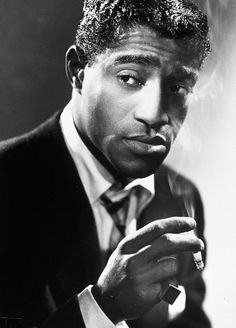
\includegraphics[width=\linewidth]{/Users/Nathaniel/Dropbox/Git/YaRrr_Book/media/sammy.jpg}
\caption{The great Sammy Davis Jr. Do yourself a favor and spend an evening watching videos of him performing on YouTube. Image used entirely without permission.}
\label{fig:sammy}
\end{marginfigure}

But before we get to making some plots, let's go over some basics on specifying colors in R:

\section{Color basics}

There are many ways to specify colors in R -- in the next chapter, I'll show you how to get really fancy with colors. But for now, let's cover two easy ways.

\begin{marginfigure}
\begin{footnotesize}
\begin{knitrout}
\definecolor{shadecolor}{rgb}{0.969, 0.969, 0.969}\color{fgcolor}\begin{kframe}
\begin{alltt}
\hlkwd{par}\hlstd{(}\hlkwc{mar} \hlstd{=} \hlkwd{c}\hlstd{(}\hlnum{0}\hlstd{,} \hlnum{0}\hlstd{,} \hlnum{0}\hlstd{,} \hlnum{0}\hlstd{))}

\hlkwd{plot}\hlstd{(}\hlkwc{x} \hlstd{=} \hlnum{1}\hlopt{:}\hlnum{11}\hlstd{,}
     \hlkwc{y} \hlstd{=} \hlkwd{rep}\hlstd{(}\hlnum{.5}\hlstd{,} \hlnum{11}\hlstd{),}
     \hlkwc{xlim} \hlstd{=} \hlkwd{c}\hlstd{(}\hlnum{1}\hlstd{,} \hlnum{11}\hlstd{),}
     \hlkwc{ylim} \hlstd{=} \hlkwd{c}\hlstd{(}\hlnum{0}\hlstd{,} \hlnum{1}\hlstd{),}
     \hlkwc{pch} \hlstd{=} \hlnum{21}\hlstd{,}
     \hlkwc{bg} \hlstd{=} \hlkwd{gray}\hlstd{(}\hlkwd{seq}\hlstd{(}\hlnum{0}\hlstd{,} \hlnum{1}\hlstd{,} \hlnum{.1}\hlstd{)),}
     \hlkwc{bty} \hlstd{=} \hlstr{"n"}\hlstd{,}
     \hlkwc{cex} \hlstd{=} \hlnum{1.6}\hlstd{,}
     \hlkwc{ylab} \hlstd{=} \hlstr{""}\hlstd{,}
     \hlkwc{xlab} \hlstd{=} \hlstr{""}\hlstd{,}
     \hlkwc{xaxt} \hlstd{=} \hlstr{"n"}\hlstd{,}
     \hlkwc{yaxt} \hlstd{=} \hlstr{"n"}
     \hlstd{)}

\hlkwd{text}\hlstd{(}\hlkwc{x} \hlstd{=} \hlnum{5.5}\hlstd{,}
     \hlkwc{y} \hlstd{=} \hlnum{.8}\hlstd{,}
     \hlkwc{labels} \hlstd{=} \hlstr{"gray(x)"}\hlstd{,}
     \hlkwc{cex} \hlstd{=} \hlnum{1.4}
     \hlstd{)}

\hlkwd{text}\hlstd{(}\hlkwc{x} \hlstd{=} \hlnum{1}\hlopt{:}\hlnum{11}\hlstd{,}
     \hlkwc{y} \hlstd{=} \hlkwd{rep}\hlstd{(}\hlnum{.5}\hlstd{,} \hlnum{11}\hlstd{),}
     \hlkwc{labels} \hlstd{=} \hlkwd{seq}\hlstd{(}\hlnum{0}\hlstd{,} \hlnum{1}\hlstd{,} \hlnum{.1}\hlstd{),}
     \hlkwc{pos} \hlstd{=} \hlnum{1}\hlstd{,}
     \hlkwc{cex} \hlstd{=} \hlnum{.8}
     \hlstd{)}
\end{alltt}
\end{kframe}
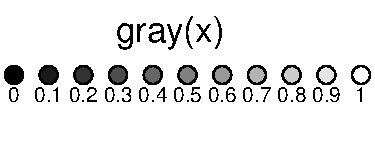
\includegraphics[width=\maxwidth]{figure/unnamed-chunk-190-1} 

\end{knitrout}
\end{footnotesize}
\end{marginfigure}


\newfun{Specifying simple colors}

\hline

\begin{description}

  \item[\tt{col = "red"}, \tt{col = "blue"}, \tt{col = "lawngreen"} (etc.)] \hfill \\

The easiest way to specify a color is to enter its name as a string. Of course, all the basic colors are there, but there are tons of quirky colors like \texttt{snow}, \texttt{papayawhip} and \texttt{lawngreen}. To see all color names in R, run the code

\begin{knitrout}
\definecolor{shadecolor}{rgb}{0.969, 0.969, 0.969}\color{fgcolor}\begin{kframe}
\begin{alltt}
\hlkwd{colors}\hlstd{()} \hlcom{# Show me all the color names!}
\end{alltt}
\end{kframe}
\end{knitrout}

  \item[\tt{col = gray(level, alpha)}] \hfill \\

The \texttt{gray()} function takes two arguments, level and alpha, and returns a shade of gray. For example, \texttt{gray(level = 1)} will return white. The alpha argument specifies how transparent to make the color on a scale from 0 (completely transparent), to 1 (not transparent at all). The default value for alpha is 1 (not transparent at all.)

\end{description}

}
}
\vspace{5mm} %5mm vertical space


\subsection{High vs. low-level plotting commands}

There are two general types of plotting commands in R: high and low-level. High level plotting commands, like \texttt{plot()}, \texttt{hist()} and \texttt{beanplot()} create entirely new plots. Within these high level plotting commands, you can define the general layout of the plot - like the axis limits and plot margins. Low level plotting commands, like \texttt{points()}, \texttt{segments()}, and \texttt{text()} add elements to existing plots. These low level commands don't change the overall layout of a plot - they just add to what you've already created. Once you are done creating a plot, you can export the plot to a pdf or jpeg using the \texttt{pdf()} or \texttt{jpeg()} functions. Or, if you're creating documents in Markdown or Latex, you can add your plot directly to your document.

\subsection{Plotting arguments}

Most plotting functions have \textit{tons} of optional arguments (also called parameters) that you can use to customize virtually everything in a plot. To see all of them, look at the help menu for \texttt{par} by executing \texttt{?par}. However, the good news is that you don't need to specify all possible parameters you create a plot. Instead, there are only a few critical arguments that you must specify - usually one or two vectors of data. For any optional arguments that you do not specify, R will use either a default value, or choose a value that makes sense based on the data you specify.

I think the best way to learn how to create plots is to see some examples. Let's start with the main high-level plotting functions.

\section{Scatterplot: \texttt{plot()}}

\begin{marginfigure}
\begin{knitrout}
\definecolor{shadecolor}{rgb}{0.969, 0.969, 0.969}\color{fgcolor}\begin{kframe}
\begin{alltt}
\hlstd{x.data} \hlkwb{<-} \hlkwd{rnorm}\hlstd{(}\hlnum{100}\hlstd{,} \hlkwc{mean} \hlstd{=} \hlnum{0}\hlstd{,} \hlkwc{sd} \hlstd{=} \hlnum{1}\hlstd{)}
\hlstd{y.data} \hlkwb{<-} \hlstd{x} \hlopt{+} \hlkwd{rnorm}\hlstd{(}\hlnum{100}\hlstd{,} \hlkwc{mean} \hlstd{=} \hlnum{0}\hlstd{,} \hlkwc{sd} \hlstd{=} \hlnum{1}\hlstd{)}

\hlkwd{plot}\hlstd{(}\hlkwc{x} \hlstd{= x.data,}
     \hlkwc{y} \hlstd{= y.data}
     \hlstd{)}
\end{alltt}
\end{kframe}
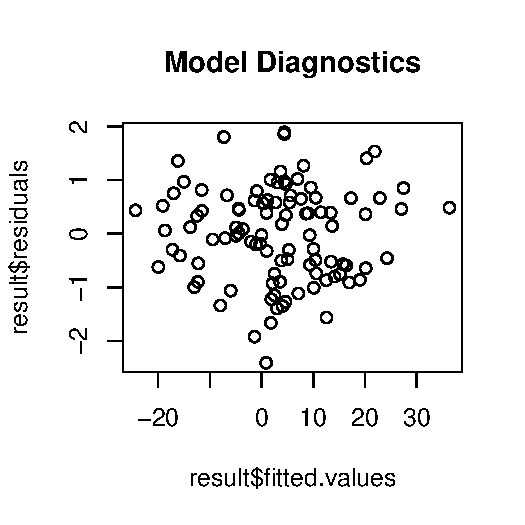
\includegraphics[width=\maxwidth]{figure/unnamed-chunk-192-1} 

\end{knitrout}

\end{marginfigure}

The most common high-level plotting function is \texttt{plot(x, y)}. While its name sounds like it can make any kind of plot, the \texttt{plot()} function actually makes a scatterplot from two vectors x and y, where the x vector indicates the x (horizontal) values of the points, and the y vector indicates the y (vertical) values. Here are the main arguments to \texttt{plot()}:

\marginnote{If you only specify one vector of data (the x argument) to the \texttt{plot()} command, R will set all the y-values to 1.}

\vspace{5mm} %5mm vertical space
\noindent
\setlength{\fboxrule}{1.5pt}
\fbox{
\parbox{\textwidth}{

\newfun{plot()}\index{plot()}

\hline

\begin{description}

  \item[\tt{x, y}] \hfill \\

  \begin{footnotesize}
  Two vectors of data indicating the horizontal (x) values, and vertical (y) values of the points. If you don't specify the y argument, R will set the y value on all points to 1.
  \end{footnotesize}


  \item[\tt{type}] \hfill \\
The type of plot. Use \texttt{type = "p"} for points (the default), \texttt{type = "l"} for lines, \texttt{type = "b"} for points and lines, and \texttt{type = "\textbackslash n"} for no plotting. Using \texttt{type = "\textbackslash n"} is helpful when you want to add plotting symbols later with low-level plotting functions.

    \item[\tt{main, xlab, ylab}] \hfill \\

      \begin{footnotesize}
String scalers indicating the text for the main plot title (\texttt{main}), the label for the horizontal x-axis (\texttt{xlab}), and the vertical y-axis (\texttt{ylab})
   \end{footnotesize}

    \item[\tt{xlim, ylim}] \hfill \\

      \begin{footnotesize}
 A numeric vector of length two containing the minimum and maximum values of the x and y-axes. For example: \texttt{xlim = c(0, 100), ylim = c(50, 60)} will set the x limits to [0, 100] and the ylimits to [50, 60].
   \end{footnotesize}

    \item[\tt{col, bg}] \hfill \\

          \begin{footnotesize}
    The color (and possibly background) of the plotting symbols. For example \texttt{col = "red"} will create red symbols. If you use a symbol with a separate background (like \texttt{pch = 21}, \texttt{bg} controls the color of the background separately from the outline.
       \end{footnotesize}

\item[\tt{pch}] \hfill \\
      \begin{footnotesize}
    An integer indicating the type of plotting symbols (see \texttt{?points} and section below), or a string specifying symbols as text. For example, \texttt{pch = 21} will create a filled circle, while \texttt{pch = "P"} will plot the character ``P''.
      \end{footnotesize}

\item[\tt{cex}] \hfill \\
          \begin{footnotesize}
  A numeric vector specifying the size of the symbols (from 0 to Inf). The default size is 1. You can enter a vector of data here to change the size of the symbols based on some data (like a third variable).
        \end{footnotesize}



\end{description}

}
}
\vspace{5mm} %5mm vertical space

As you can see, the \texttt{plot()} function, like many plotting functions, has several optional arguments that allow you to change aspects of the plot. There are so many ways to customize the look of a plot that the number of optional arguments can be overwhelming at first. Let's start by looking at an example of a simple scatterplot showing ten data points: [1, 1], [2, 2] ... [10, 10].

\begin{footnotesize}
\begin{knitrout}
\definecolor{shadecolor}{rgb}{0.969, 0.969, 0.969}\color{fgcolor}\begin{kframe}
\begin{alltt}
\hlkwd{plot}\hlstd{(}\hlkwc{x} \hlstd{=} \hlnum{1}\hlopt{:}\hlnum{10}\hlstd{,} \hlcom{# x-coordinates}
     \hlkwc{y} \hlstd{=} \hlnum{1}\hlopt{:}\hlnum{10}\hlstd{,} \hlcom{# y-coordinates}
     \hlkwc{main} \hlstd{=} \hlstr{"My First Plot"}\hlstd{,}
     \hlkwc{xlab} \hlstd{=} \hlstr{"This is the x-axis label"}\hlstd{,}
     \hlkwc{ylab} \hlstd{=} \hlstr{"This is the y-axis label"}\hlstd{,}
     \hlkwc{xlim} \hlstd{=} \hlkwd{c}\hlstd{(}\hlnum{0}\hlstd{,} \hlnum{11}\hlstd{),} \hlcom{# Min and max values for x-axis}
     \hlkwc{ylim} \hlstd{=} \hlkwd{c}\hlstd{(}\hlnum{0}\hlstd{,} \hlnum{11}\hlstd{),} \hlcom{# Min and max values for y-axis}
     \hlkwc{col} \hlstd{=} \hlstr{"blue"}\hlstd{,} \hlcom{# Color of the points}
     \hlkwc{pch} \hlstd{=} \hlnum{16}\hlstd{,} \hlcom{# Type of symbol (16 means Filled circle)}
     \hlkwc{cex} \hlstd{=} \hlnum{1} \hlcom{# Size of the symbols}
     \hlstd{)}
\end{alltt}
\end{kframe}

{\centering 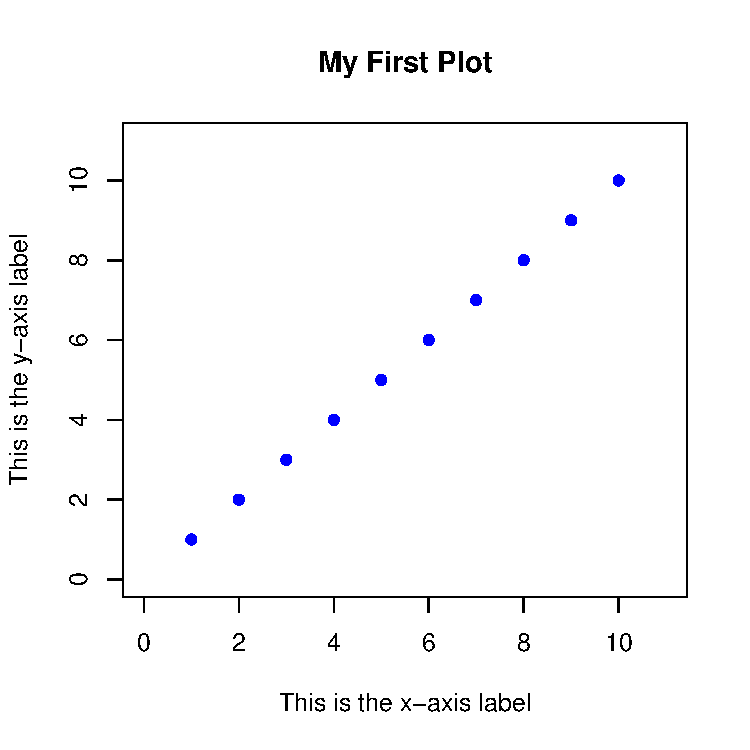
\includegraphics[width=\maxwidth]{figure/unnamed-chunk-193-1} 

}



\end{knitrout}
\end{footnotesize}


Aside from the x and y arguments, all of the arguments are optional. If you don't specify a specific argument, then R will use a default value, or try to come up with a value that makes sense. For example, if you don't specify the \texttt{xlim} and \texttt{ylim} arguments, R will set the limits so that all the points fit inside the plot.

\subsection{Symbol types: pch}


\begin{marginfigure}
\begin{tiny}
\begin{knitrout}
\definecolor{shadecolor}{rgb}{0.969, 0.969, 0.969}\color{fgcolor}\begin{kframe}
\begin{alltt}
\hlkwd{par}\hlstd{(}\hlkwc{mar}  \hlstd{=} \hlkwd{rep}\hlstd{(}\hlnum{0}\hlstd{,} \hlnum{4}\hlstd{))}

\hlkwd{plot}\hlstd{(}\hlkwc{x} \hlstd{=} \hlkwd{rep}\hlstd{(}\hlnum{1}\hlopt{:}\hlnum{5}\hlstd{,} \hlkwc{each} \hlstd{=} \hlnum{5}\hlstd{),}
     \hlkwc{y} \hlstd{=} \hlkwd{rep}\hlstd{(}\hlnum{5}\hlopt{:}\hlnum{1}\hlstd{,} \hlkwc{times} \hlstd{=} \hlnum{5}\hlstd{),}
     \hlkwc{pch} \hlstd{=} \hlnum{1}\hlopt{:}\hlnum{25}\hlstd{,}
     \hlkwc{xlab} \hlstd{=} \hlstr{""}\hlstd{,} \hlkwc{ylab} \hlstd{=} \hlstr{""}\hlstd{,} \hlkwc{xaxt} \hlstd{=} \hlstr{"n"}\hlstd{,} \hlkwc{yaxt} \hlstd{=} \hlstr{"n"}\hlstd{,}
     \hlkwc{xlim} \hlstd{=} \hlkwd{c}\hlstd{(}\hlnum{.5}\hlstd{,} \hlnum{5.5}\hlstd{),}
     \hlkwc{ylim} \hlstd{=} \hlkwd{c}\hlstd{(}\hlnum{0}\hlstd{,} \hlnum{6}\hlstd{),}
     \hlkwc{bty} \hlstd{=} \hlstr{"n"}\hlstd{,} \hlkwc{bg} \hlstd{=} \hlstr{"gray"}\hlstd{,} \hlkwc{cex} \hlstd{=} \hlnum{1.4}
     \hlstd{)}

\hlkwd{text}\hlstd{(}\hlkwc{x} \hlstd{=} \hlkwd{rep}\hlstd{(}\hlnum{1}\hlopt{:}\hlnum{5}\hlstd{,} \hlkwc{each} \hlstd{=} \hlnum{5}\hlstd{)} \hlopt{-} \hlnum{.35}\hlstd{,}
     \hlkwc{y} \hlstd{=} \hlkwd{rep}\hlstd{(}\hlnum{5}\hlopt{:}\hlnum{1}\hlstd{,} \hlkwc{times} \hlstd{=} \hlnum{5}\hlstd{),}
     \hlkwc{labels} \hlstd{=} \hlnum{1}\hlopt{:}\hlnum{25}\hlstd{,} \hlkwc{cex} \hlstd{=} \hlnum{1.2}
     \hlstd{)}
\end{alltt}
\end{kframe}
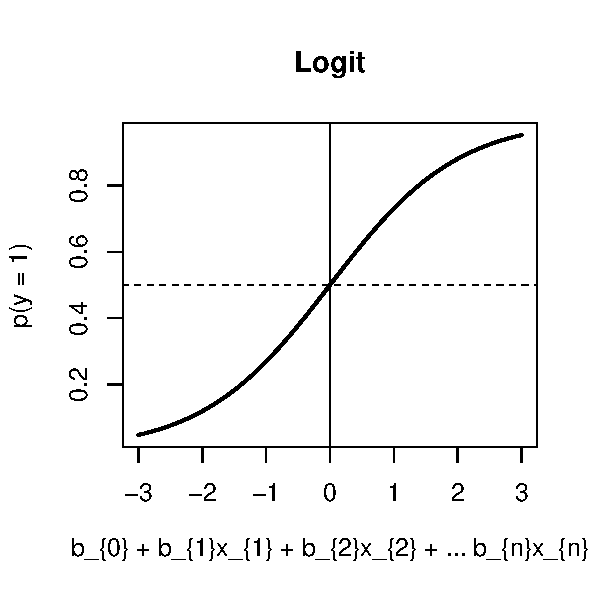
\includegraphics[width=\maxwidth]{figure/unnamed-chunk-194-1} 

\end{knitrout}
\end{tiny}
\caption{The symbol types associated with the \texttt{pch} plotting parameter.}
\label{fig:pchplot}
\end{marginfigure}


When you create a plot with \texttt{plot(x, y)}, you can specify the type of symbol with the \texttt{pch} argument. You can specify the symbol type in one of two ways: with an integer, or with a string. If you use a string (like \texttt{"p"}), R will use that text as the plotting symbol. If you use an integer value, you'll get the symbol that correspond to that number. See Figure~\ref{fig:pchplot} in the margin.

Symbols differ in their border shape and how the filling is done. Symbols 1 through 14 only have borders and are always empty, while symbols 15 through 20 don't have a border and are always filled. Symbols 21 through 25 have both a border and a filling.

To specify the border color for all symbols, use the \texttt{col} argument. For symbols 21 through 25, you can additionally set the color of the fill using the \texttt{bg} ("background") argument.



\subsection{Scatterplot of pirates data}

In our first plot above, we just plotted the integers from 1 to 10. Of course, we can also plot vectors from columns in dataframes! Let's create a scatterplot from the pirates dataset. We'll put the pirate's age on the x-axis, and the number of treasure chests he/she has found on the y-axis. I'll add a few extra arguments like xlim and ylim to make the plot a bit wider than the default size. I'll also set the color of the points to be transparent gray (\texttt{col = gray(level = .1, alpha = .2)}) -- this will show us where there are many points on top of each other.

\marginnote{As you can see in our plotting commands, we did not specify parameters like \texttt{xlim} and \texttt{ylim}. If you don't specify these arguments, R will try to come up with values that make sense given the data.}

\begin{knitrout}
\definecolor{shadecolor}{rgb}{0.969, 0.969, 0.969}\color{fgcolor}\begin{kframe}
\begin{alltt}
\hlkwd{plot}\hlstd{(}\hlkwc{x} \hlstd{= pirates}\hlopt{$}\hlstd{age,}
     \hlkwc{y} \hlstd{= pirates}\hlopt{$}\hlstd{tchests,}
     \hlkwc{xlab} \hlstd{=} \hlstr{"Age"}\hlstd{,}
     \hlkwc{ylab} \hlstd{=} \hlstr{"Treasure Chests Found"}\hlstd{,}
     \hlkwc{main} \hlstd{=} \hlstr{"Pirate data"}\hlstd{,}
     \hlkwc{pch} \hlstd{=} \hlnum{16}\hlstd{,} \hlcom{# 24 are filled triangles,}
     \hlkwc{xlim} \hlstd{=} \hlkwd{c}\hlstd{(}\hlnum{10}\hlstd{,} \hlnum{50}\hlstd{),}
     \hlkwc{ylim} \hlstd{=} \hlkwd{c}\hlstd{(}\hlnum{0}\hlstd{,} \hlnum{60}\hlstd{),}
     \hlkwc{col} \hlstd{=} \hlkwd{gray}\hlstd{(}\hlkwc{level} \hlstd{=} \hlnum{.1}\hlstd{,} \hlkwc{alpha} \hlstd{=} \hlnum{.1}\hlstd{)}
     \hlstd{)}
\end{alltt}
\end{kframe}
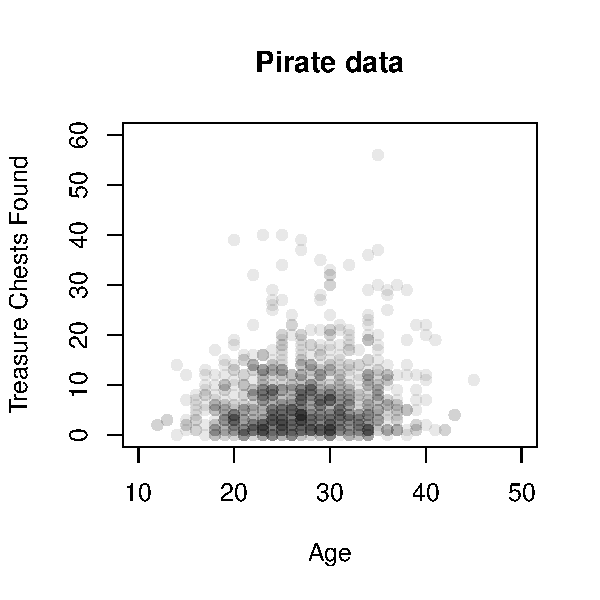
\includegraphics[width=\maxwidth]{figure/unnamed-chunk-195-1} 

\end{knitrout}

It looks like most of the points are between the ages of 20 and 30 with between 0 and 10 treasure chests found!

\section{Histogram: \texttt{hist()}}

Histograms are the most common way to plot unidimensional numeric data. To create a histogram we'll use the \texttt{hist()} function:

\vspace{5mm} %5mm vertical space
\noindent
\setlength{\fboxrule}{1.5pt}
\fbox{
\parbox{\textwidth}{

\newfun{hist()}\index{hist()}

\hline

\begin{description}

  \item[\tt{x}] \hfill \\
  A vector of numeric data
    \item[\tt{breaks}] \hfill \\
 One of several values that defines how bins are created. The most common argument is a single number giving the number of bins you want in the histogram. See \texttt{?hist} for additional ways to specify this.
    \item[\tt{col, border}] \hfill \\
    The color of the filling (col) and border (border) of the bars.
\item[\tt{main, xlab, ylab, xlim, ylim ...}] \hfill \\
    Other standard plotting arguments

\end{description}

}
}
\vspace{5mm} %5mm vertical space

Let's create a histogram of the ages of pirates in the \texttt{pirates} dataset:

\begin{knitrout}
\definecolor{shadecolor}{rgb}{0.969, 0.969, 0.969}\color{fgcolor}\begin{kframe}
\begin{alltt}
\hlkwd{hist}\hlstd{(}\hlkwc{x} \hlstd{= pirates}\hlopt{$}\hlstd{age,}
     \hlkwc{main} \hlstd{=} \hlstr{"Pirate Ages"}\hlstd{,}
     \hlkwc{xlab} \hlstd{=} \hlstr{"Age"}\hlstd{,}
     \hlkwc{ylab} \hlstd{=} \hlstr{"Frequency"}
     \hlstd{)}
\end{alltt}
\end{kframe}
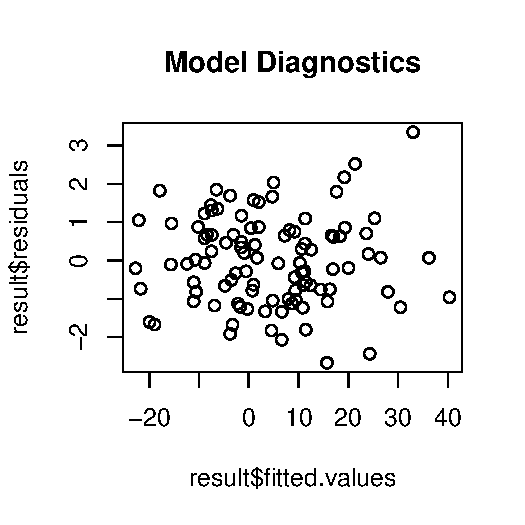
\includegraphics[width=\maxwidth]{figure/unnamed-chunk-196-1} 

\end{knitrout}

We can get more fancy by adding additional arguments (see the margin figure \ref{fig:piratehist})


\begin{marginfigure}

\begin{knitrout}
\definecolor{shadecolor}{rgb}{0.969, 0.969, 0.969}\color{fgcolor}\begin{kframe}
\begin{alltt}
\hlkwd{hist}\hlstd{(}\hlkwc{x} \hlstd{= pirates}\hlopt{$}\hlstd{age,}
     \hlkwc{main} \hlstd{=} \hlstr{"Pirate Ages"}\hlstd{,}
     \hlkwc{xlab} \hlstd{=} \hlstr{"Age"}\hlstd{,}
     \hlkwc{ylab} \hlstd{=} \hlstr{"Frequency"}\hlstd{,}
     \hlkwc{breaks} \hlstd{=} \hlnum{20}\hlstd{,} \hlcom{# 20 Bins}
     \hlkwc{xlim} \hlstd{=} \hlkwd{c}\hlstd{(}\hlnum{0}\hlstd{,} \hlnum{60}\hlstd{),}
     \hlkwc{col} \hlstd{=} \hlstr{"papayawhip"}\hlstd{,} \hlcom{# Filling Color}
     \hlkwc{border} \hlstd{=} \hlstr{"hotpink"} \hlcom{# Border Color}
     \hlstd{)}
\end{alltt}
\end{kframe}
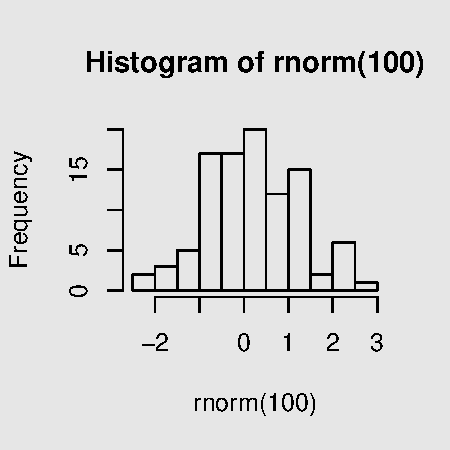
\includegraphics[width=\maxwidth]{figure/unnamed-chunk-197-1} 

\end{knitrout}
\label{fig:piratehist}
\end{marginfigure}


You can see an example of a histogram in the margin Figure~\ref{fig:histogram}.


\section{The Pirate Plot: \texttt{pirateplot()}}

The last high-level plotting function I want to show you is the \texttt{pirateplot()} function. The best part of a pirate plot is that it shows you three aspects of data: Raw data, Descriptive Statistics, and Inferential Statistics. Plus, as you can see in Figure~\ref{fig:beanplot}, they look much, much cooler than a boxplot or histogram. This means that you can quickly detect outliers, multiple modes, or missing data much better than you can with boxplots.

The \texttt{pirateplot()} function is part of the yarrr package. So to use it, you'll first need to load the yarrr package

\begin{footnotesize}
\begin{knitrout}
\definecolor{shadecolor}{rgb}{0.969, 0.969, 0.969}\color{fgcolor}\begin{kframe}
\begin{alltt}
\hlkwd{library}\hlstd{(yarrr)}
\end{alltt}
\end{kframe}
\end{knitrout}
\end{footnotesize}

Here are some of the main arguments for \texttt{pirateplot()}. Check out the help menu (\texttt{?pirateplot}) to see several additional arguments

\vspace{5mm} %5mm vertical space
\noindent
\setlength{\fboxrule}{1.5pt}
\fbox{
\parbox{\textwidth}{

\newfun{pirateplot()}\index{pirateplot()}

\hline

\begin{description}

  \item[\tt{dv.name, iv.name}] \hfill \\
     Two string values indicating the names of the dependent variable and the independent variables in a dataframe.

        \item[\tt{data}] \hfill \\
  A dataframe with columns corresponding to dv.name and iv.name. If you want to use a subset of data from a dataframe, just include the \texttt{subset()} function within this argument (e.g.; \texttt{data = subset(pirates, gender == "male")})


\item[\tt{add.hdi}] \hfill \\
A logical value indicating whether or not to add a 95\% highest density interval (HDI) to the plot. This is a Bayesian interval which, assuming t-distributed data, gives you a 95\% Bayesian posterior interval for the location of the population mean.

\item[\tt{labels}] \hfill \\
An optional string vector specifying the names of groups (levels of the IV)

\item[\tt{my.palette}] \hfill \\

A string (or vector of strings) indicating the colors of the beans. This can either be the name of a color palette in the piratepal function (run \texttt{piratepal(action = "p")} to see the names of all the palettes), or a vector of strings referring to colors. For example, \texttt{my.palette = "black"} will create a gray-scale plot.

\item[\tt{trans.vec}] \hfill \\

A numeric vector of 5 values between 0 and 1 that indicate how transparent to make the colors in each distribution The five numbers correspond to the points, bean outlines, hdi band, the average line, and the white background respectively. For example, \texttt{trans.vec = c(1, 0, 0, 0, 0)} will only plot the raw data.


\item[\tt{...}] \hfill \\
Other arguments passed on to the plot function (e.g.; main, xlab, ylab, ylim)

\end{description}

}
}
\vspace{5mm} %5mm vertical space

The code for creating pirateplots is a bit different from scatterplots with \texttt{plot()} and histograms with \texttt{hist()}. Let's start with an example: I'll create a pirateplot using a new dataset called \texttt{BeardLengths}. This dataset shows the length of 100 pirates' beards on three different ships: the Angry Badger, the Fearless Snake, and the Nervous Goat:

\begin{marginfigure}

You can can easily customize the look of your pirate plot with additional arguments. For example, to make a black and white plot with a stronger focus on the raw data, set \texttt{my.palette = "black"} and \texttt{trans.vec = c(.2, .8, .8, .8, .8, .8)}:

\begin{footnotesize}
\begin{knitrout}
\definecolor{shadecolor}{rgb}{0.969, 0.969, 0.969}\color{fgcolor}\begin{kframe}
\begin{alltt}
\hlkwd{library}\hlstd{(}\hlstr{"yarrr"}\hlstd{)}

\hlkwd{pirateplot}\hlstd{(}\hlkwc{dv.name} \hlstd{=} \hlstr{"Beard"}\hlstd{,}
           \hlkwc{iv.name} \hlstd{=} \hlstr{"Ship"}\hlstd{,}
         \hlkwc{data} \hlstd{= BeardLengths,}
         \hlkwc{my.palette} \hlstd{=} \hlstr{"black"}\hlstd{,}
         \hlkwc{trans.vec} \hlstd{=} \hlkwd{c}\hlstd{(}\hlnum{.2}\hlstd{,} \hlnum{.8}\hlstd{,} \hlnum{.8}\hlstd{,} \hlnum{.8}\hlstd{,} \hlnum{.8}\hlstd{),}
         \hlkwc{main} \hlstd{=} \hlstr{"My First Pirate Plot!"}\hlstd{,}
         \hlkwc{xlab} \hlstd{=} \hlstr{"Favorite Pirate"}\hlstd{,}
         \hlkwc{ylab} \hlstd{=} \hlstr{"# of Tattoos"}
         \hlstd{)}
\end{alltt}
\end{kframe}
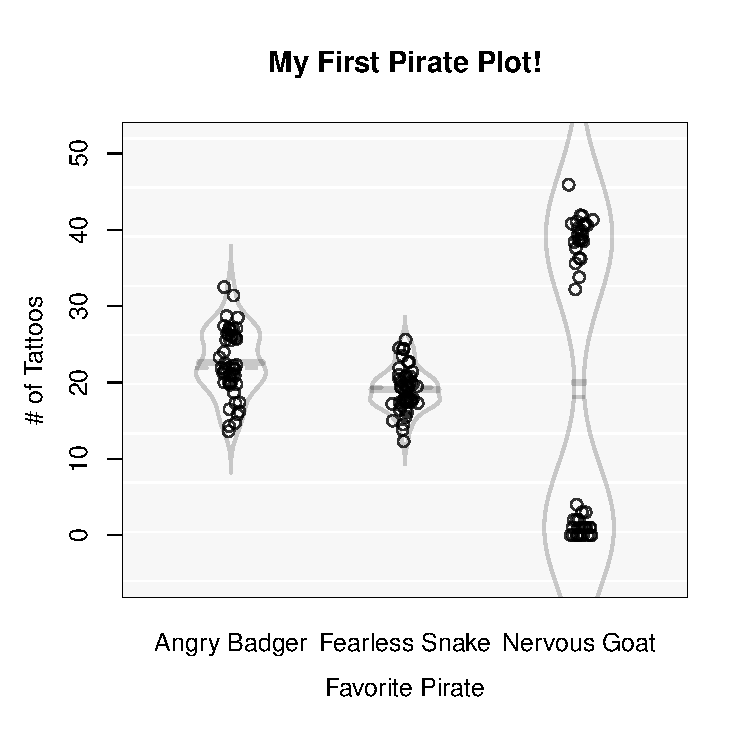
\includegraphics[width=\maxwidth]{figure/unnamed-chunk-199-1} 

\end{knitrout}
\end{footnotesize}


\end{marginfigure}

\begin{footnotesize}
\begin{knitrout}
\definecolor{shadecolor}{rgb}{0.969, 0.969, 0.969}\color{fgcolor}\begin{kframe}
\begin{alltt}
\hlkwd{library}\hlstd{(}\hlstr{"yarrr"}\hlstd{)}

\hlkwd{pirateplot}\hlstd{(}\hlkwc{dv.name} \hlstd{=} \hlstr{"Beard"}\hlstd{,}
           \hlkwc{iv.name} \hlstd{=} \hlstr{"Ship"}\hlstd{,}
         \hlkwc{data} \hlstd{= BeardLengths,}
         \hlkwc{main} \hlstd{=} \hlstr{"My First Pirate Plot!"}\hlstd{,}
         \hlkwc{xlab} \hlstd{=} \hlstr{"Favorite Pirate"}\hlstd{,}
         \hlkwc{ylab} \hlstd{=} \hlstr{"# of Tattoos"}
         \hlstd{)}
\end{alltt}
\end{kframe}
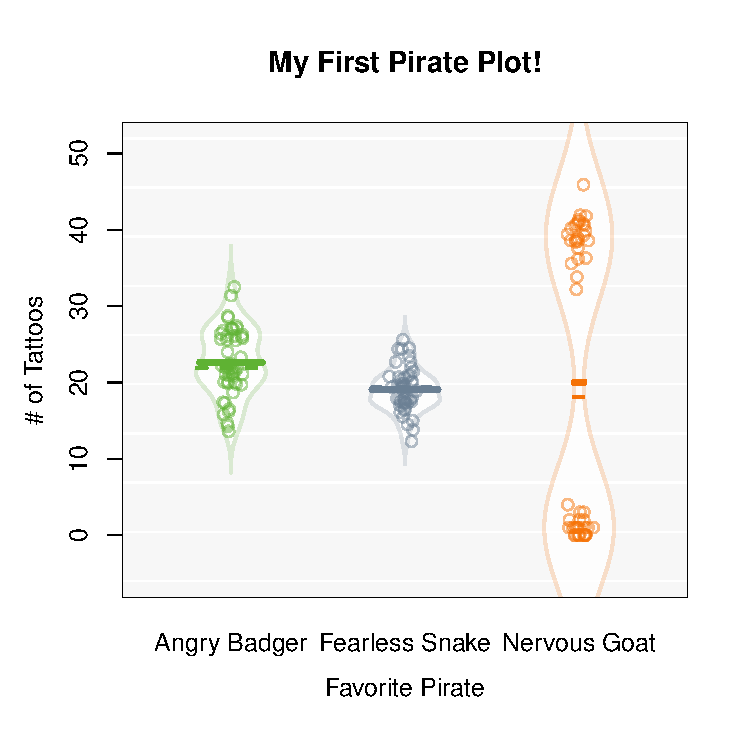
\includegraphics[width=\maxwidth]{figure/unnamed-chunk-200-1} 

\end{knitrout}
\end{footnotesize}




Let's walk through the main arguments. First, in the \texttt{dv.name} and \texttt{iv.name} arguments, we specify the names of the dependent and independent variables in the dataset that we want to plot as strings. Next, in the \texttt{data} argument we specify the dataframe object that contains the data. Finally, we can specify some plotting labels like \texttt{main}, \texttt{xlab} and \texttt{ylab} just like in \texttt{plot()}.



\section{Other plotting types}

Compared to pirate plots, these next two plotting types, barplots and boxplots, are pretty boring. But if you want to make them, here's how:

\subsection{Barplot: barplot()}

A barplot shows a single bar representing a single value for every level of some independent variable. Here are the main arguments to \texttt{barplot()}

\marginnote{As always, check the help menu for barplots with \texttt{?barplot} for additional arguments and examples}


\vspace{5mm} %5mm vertical space
\noindent
\setlength{\fboxrule}{1.5pt}
\fbox{
\parbox{\textwidth}{

\newfun{barplot()}\index{barplot}

\hline

\begin{description}

  \item[\tt{height}] \hfill \\
     A numeric vector indicating the heights of the bars
        \item[\tt{names.arg}] \hfill \\
 An optional string vector indicating the names under the bars
         \item[\tt{border, col}] \hfill \\
    The color of the borders (\texttt{border}) and filling (\texttt{col}) of the bars.
        \item[\tt{main, xlab, ylab}] \hfill \\
Optional string values indicating the main and sub-titles, and axis labels of the plot

\end{description}

}
}
\vspace{5mm} %5mm vertical space

\begin{knitrout}
\definecolor{shadecolor}{rgb}{0.969, 0.969, 0.969}\color{fgcolor}\begin{kframe}
\begin{alltt}
\hlkwd{barplot}\hlstd{(}\hlkwc{height} \hlstd{=} \hlnum{1}\hlopt{:}\hlnum{5}\hlstd{,}
        \hlkwc{names.arg} \hlstd{=} \hlkwd{c}\hlstd{(}\hlstr{"Name 1"}\hlstd{,} \hlstr{"Name 2"}\hlstd{,} \hlstr{"Name 3"}\hlstd{,} \hlstr{"Name 4"}\hlstd{,} \hlstr{"Name 5"}\hlstd{),}
        \hlkwc{main} \hlstd{=} \hlstr{"My first barplot"}\hlstd{,}
        \hlkwc{xlab} \hlstd{=} \hlstr{"IV"}\hlstd{,}
        \hlkwc{ylab} \hlstd{=} \hlstr{"DV"}
        \hlstd{)}
\end{alltt}
\end{kframe}
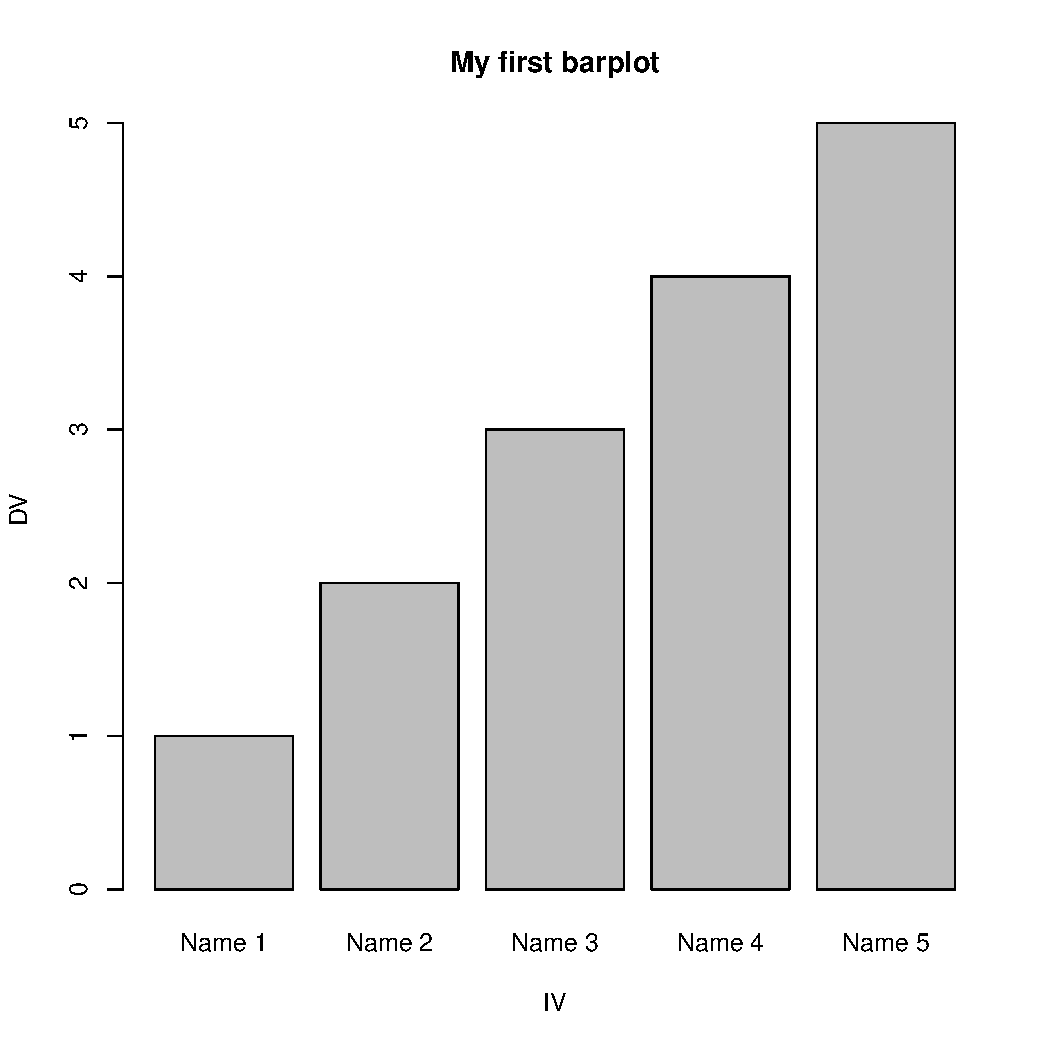
\includegraphics[width=\maxwidth]{figure/unnamed-chunk-201-1} 

\end{knitrout}


\subsection{Boxplot: boxplot()}

Boxplots aren't used so often anymore, but if you want to be old-school, they're a good place to start. To create a boxplot, use the \texttt{boxplot()} function:



\vspace{5mm} %5mm vertical space
\noindent
\setlength{\fboxrule}{1.5pt}
\fbox{
\parbox{\textwidth}{

\newfun{boxplot()}\index{boxplot()}

\hline

\begin{description}

  \item[\tt{formula, data}] \hfill \\
      A formula in the form \texttt{formula = dv {\raise.17ex\hbox{$\scriptstyle\sim$}} iv} indicating the dependent variable and independent variable, and a dataframe containing the variables in the formula. For example \texttt{formula = height {\raise.17ex\hbox{$\scriptstyle\sim$}} sex}
        \item[\tt{subset}] \hfill \\
  An optional logical vector indicating a subset of the data to plot. For example, the command \texttt{subset = gender == "male" \& weight < 120}, will only plot data for males with weight less than 120.
         \item[\tt{border, col}] \hfill \\
    The color of the borders (\texttt{border}) and filling (\texttt{col}) of the boxes.
        \item[\tt{names}] \hfill \\
      A string vector indicating the names of the boxes. E.g.; \texttt{names = c("males", "females")}

\end{description}

}
}
\vspace{5mm} %5mm vertical space


\begin{marginfigure}
\begin{knitrout}
\definecolor{shadecolor}{rgb}{0.969, 0.969, 0.969}\color{fgcolor}\begin{kframe}
\begin{alltt}
\hlkwd{boxplot}\hlstd{(}\hlkwc{x} \hlstd{= pirates}\hlopt{$}\hlstd{age,}
        \hlkwc{names} \hlstd{=} \hlstr{"All Data"}\hlstd{,}
        \hlkwc{ylab} \hlstd{=} \hlstr{"Age"}\hlstd{,}
        \hlkwc{main} \hlstd{=} \hlstr{"Plot 1: All Ages"}\hlstd{)}
\end{alltt}
\end{kframe}
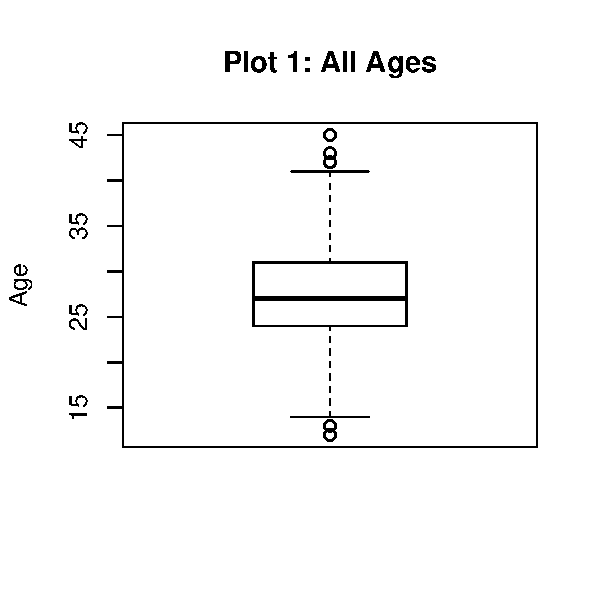
\includegraphics[width=\maxwidth]{figure/unnamed-chunk-202-1} 

\end{knitrout}

\caption{Plotting data from a single vector}
\label{fig:boxplot1}
\end{marginfigure}

\begin{marginfigure}
\begin{knitrout}
\definecolor{shadecolor}{rgb}{0.969, 0.969, 0.969}\color{fgcolor}\begin{kframe}
\begin{alltt}
\hlkwd{boxplot}\hlstd{(age} \hlopt{~} \hlstd{college,} \hlcom{# Formula: DV ~ IV is Diet}
        \hlkwc{data} \hlstd{= pirates,}
        \hlkwc{xlab} \hlstd{=} \hlstr{"college"}\hlstd{,}
        \hlkwc{ylab} \hlstd{=} \hlstr{"Weight"}\hlstd{,}
        \hlkwc{main} \hlstd{=} \hlstr{"Plot 2: Age separated by college"}\hlstd{)}
\end{alltt}
\end{kframe}
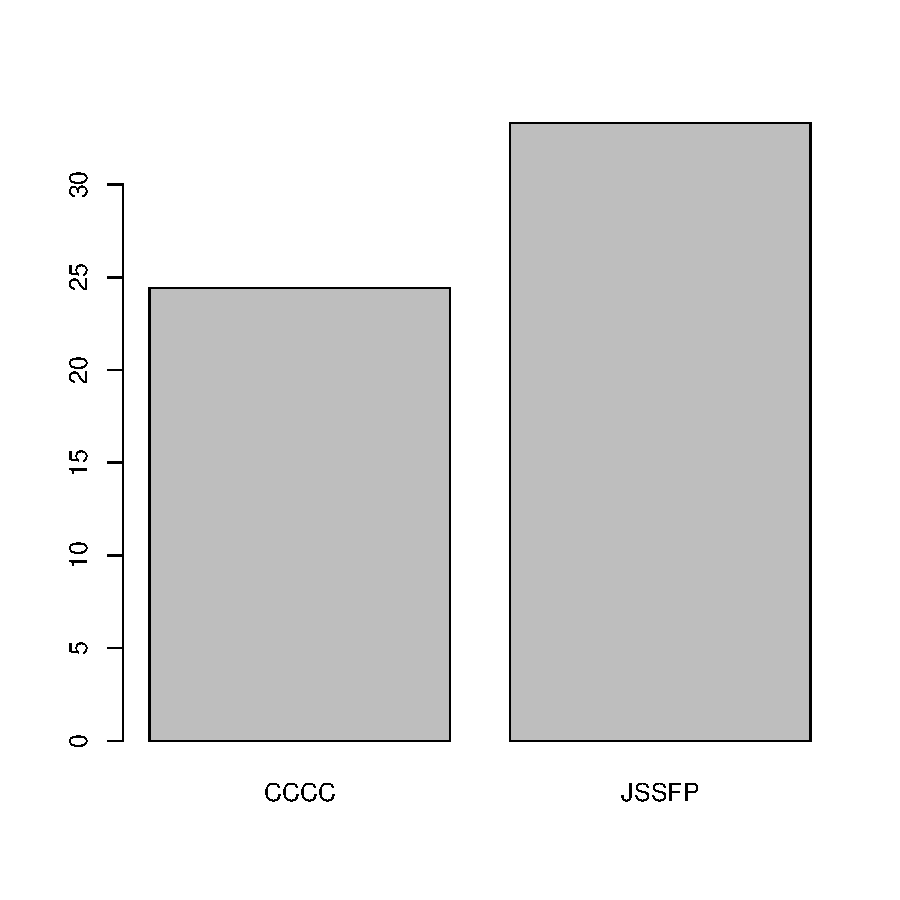
\includegraphics[width=\maxwidth]{figure/unnamed-chunk-203-1} 

\end{knitrout}

\caption{Plotting data as a function of levels of an independent variable using the \texttt{y {\raise.17ex\hbox{$\scriptstyle\sim$}} x} formula notation.}
\label{fig:boxplot2}
\end{marginfigure}

When you use \texttt{boxplot()}, you can either specify a single vector of data to plot, or you can use a \texttt{formula} to indicate a dependent and independent variable. If you do this, R will add separate boxes for all values of the independent variable.

Let's go through two examples of boxplots in Figure~\ref{fig:boxplot}. In the first plot, I just entered a single vector of data: \texttt{pirates\$age} representing all weight data in the dataframe. In the second plot, I plotted separate boxes for the different levels of \texttt{college} using the formula notation \texttt{age {\raise.17ex\hbox{$\scriptstyle\sim$}} college}. If you're wondering how R knows that I'm referring to the \texttt{pirates} dataframe when using the formula notation, the answer is that I had to specify the name of the dataframe \texttt{pirates} as an additional \texttt{data} argument. This argument tells R that the objects in the formula are names in the \texttt{pirates} dataframe.



\section{Low-level plotting functions}

Once you've created a plot with a high-level plotting function, you can add additional elements, like additional data points, reference lines, text, and legends using low-level plotting functions. There are many low-level plotting functions, I will focus on those that I frequently use.

\subsection{Starting with a blank plot}


\begin{marginfigure}
\begin{tiny}
\begin{knitrout}
\definecolor{shadecolor}{rgb}{0.969, 0.969, 0.969}\color{fgcolor}\begin{kframe}
\begin{alltt}
\hlcom{# Create a blank plot}
\hlkwd{plot}\hlstd{(}\hlkwc{x} \hlstd{=} \hlnum{1}\hlstd{,}
     \hlkwc{xlab} \hlstd{=} \hlstr{""}\hlstd{,}
     \hlkwc{ylab} \hlstd{=} \hlstr{""}\hlstd{,}
     \hlkwc{xaxt} \hlstd{=} \hlstr{"n"}\hlstd{,} \hlkwc{yaxt} \hlstd{=} \hlstr{"n"}\hlstd{,}
     \hlkwc{type} \hlstd{=} \hlstr{"n"}\hlstd{,}
     \hlkwc{xlim} \hlstd{=} \hlkwd{c}\hlstd{(}\hlnum{0}\hlstd{,} \hlnum{100}\hlstd{),} \hlkwc{ylim} \hlstd{=} \hlkwd{c}\hlstd{(}\hlnum{0}\hlstd{,} \hlnum{100}\hlstd{),}
     \hlkwc{main} \hlstd{=} \hlstr{"Blank Plot"}\hlstd{)}
\end{alltt}
\end{kframe}
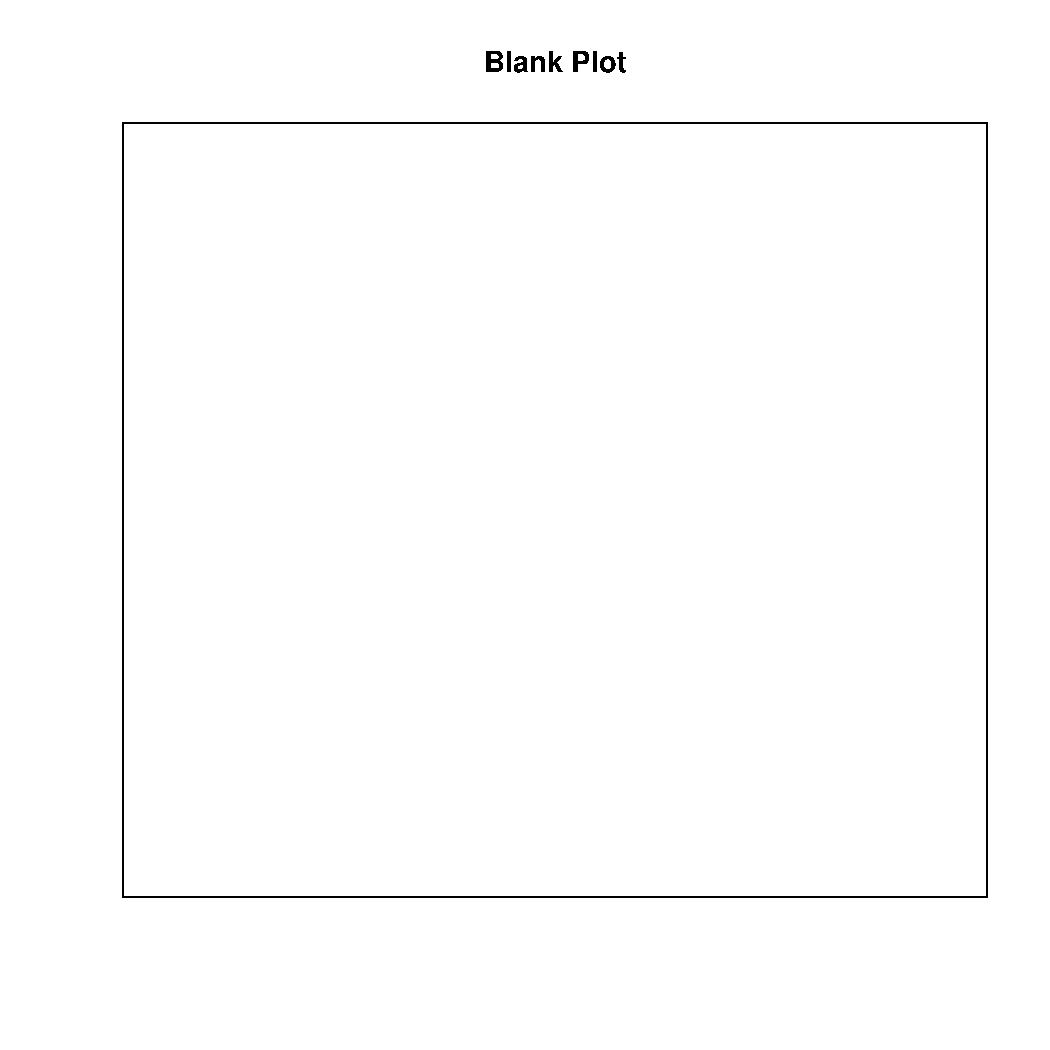
\includegraphics[width=\maxwidth]{figure/unnamed-chunk-204-1} 

\end{knitrout}
\end{tiny}
\caption{A blank plot. Useful to start with before adding elements with low-level plotting commands. Just make sure to set the axis limits to values that make sense for your future data.}
\label{fig:blankplot}
\end{marginfigure}

I like using low-level plotting functions so much that I frequently like to start with a (mostly) blank plotting space, and then add the main plot elements using low-level plotting functions. To start with a blank plot, use the \texttt{plot()} function combined with the arguments \texttt{type = "n", xaxt = "n", yaxt = "n"} and all labels set to \texttt{""}. See margin Figure~\ref{fig:blankplot} for an example

Once you've created a blank plot, you can proceed to add all the elements you'd like with low-level plotting commands. Let's start with \texttt{points()}, which adds points to an existing plot

\section{points()}


\begin{marginfigure}
\begin{tiny}
\begin{knitrout}
\definecolor{shadecolor}{rgb}{0.969, 0.969, 0.969}\color{fgcolor}\begin{kframe}
\begin{alltt}
\hlcom{# Get subsets of data}
\hlstd{college.1} \hlkwb{<-} \hlkwd{subset}\hlstd{(pirates, college} \hlopt{==} \hlstr{"CCCC"}\hlstd{)}
\hlstd{college.2} \hlkwb{<-} \hlkwd{subset}\hlstd{(pirates, college} \hlopt{==} \hlstr{"JSSFP"}\hlstd{)}

\hlcom{# Create a blank plot}
\hlkwd{plot}\hlstd{(}\hlkwc{x} \hlstd{=} \hlnum{1}\hlstd{,}
     \hlkwc{xlab} \hlstd{=} \hlstr{"Age"}\hlstd{,}
     \hlkwc{ylab} \hlstd{=} \hlstr{"Number of Tattoos"}\hlstd{,}
     \hlkwc{type} \hlstd{=} \hlstr{"n"}\hlstd{,}
     \hlkwc{main} \hlstd{=} \hlstr{"Pirate Tattoos by college"}\hlstd{,}
     \hlkwc{xlim} \hlstd{=} \hlkwd{c}\hlstd{(}\hlnum{1}\hlstd{,} \hlnum{50}\hlstd{),}
     \hlkwc{ylim} \hlstd{=} \hlkwd{c}\hlstd{(}\hlnum{0}\hlstd{,} \hlnum{20}\hlstd{))}

\hlcom{# Add red points for college 1}
\hlkwd{points}\hlstd{(}\hlkwc{x} \hlstd{= college.1}\hlopt{$}\hlstd{age,}
       \hlkwc{y} \hlstd{= college.1}\hlopt{$}\hlstd{tattoos,}
       \hlkwc{pch} \hlstd{=} \hlnum{16}\hlstd{,}
       \hlkwc{col} \hlstd{=} \hlstr{"red"}\hlstd{)}

\hlcom{# Add skyblue points for diet 2}
\hlkwd{points}\hlstd{(}\hlkwc{x} \hlstd{= college.2}\hlopt{$}\hlstd{age,}
       \hlkwc{y} \hlstd{= college.2}\hlopt{$}\hlstd{tattoos,}
       \hlkwc{pch} \hlstd{=} \hlnum{16}\hlstd{,}
       \hlkwc{col} \hlstd{=} \hlstr{"skyblue"}\hlstd{)}
\end{alltt}
\end{kframe}
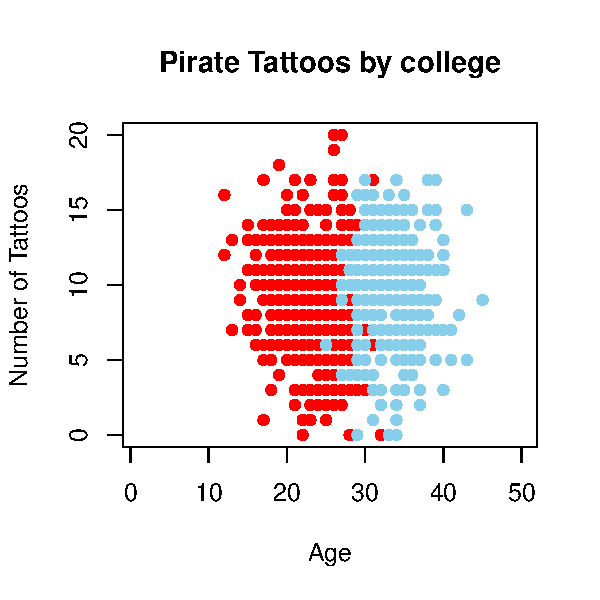
\includegraphics[width=\maxwidth]{figure/unnamed-chunk-205-1} 

\end{knitrout}
\caption{Adding additional points to an existing plot with points()}
\label{pointsexample}
\end{tiny}
\end{marginfigure}


\vspace{5mm} %5mm vertical space
\noindent
\setlength{\fboxrule}{1.5pt}
\fbox{
\parbox{\textwidth}{

\newfun{points()}\index{points()}

\hline

\begin{description}

\item[\tt{x, y}] \hfill \\
Two vectors corresponding to the x and y values of the points

\item[\tt{pch, col, bg}] \hfill \\
Type of plotting symbols (\texttt{pch}), color of the plotting symbols (\texttt{col}), and the color of the filling of the plotting symbols ((\texttt{bg})) for plotting symbols 21 through 25


\end{description}

}
}
\vspace{5mm} %5mm vertical space


For example, to add red circle points to a plot where \texttt{x.vals} are the x-values and \texttt{y.vals} are the y.values, you can run the code:

\begin{knitrout}
\definecolor{shadecolor}{rgb}{0.969, 0.969, 0.969}\color{fgcolor}\begin{kframe}
\begin{alltt}
\hlkwd{points}\hlstd{(}\hlkwc{x} \hlstd{= x.vals,} \hlcom{# x-values}
       \hlkwc{y} \hlstd{= y.vals,} \hlcom{# y-values}
       \hlkwc{col} \hlstd{=} \hlstr{"red"}\hlstd{,} \hlcom{# Symbol color}
       \hlkwc{pch} \hlstd{=} \hlnum{16} \hlcom{# Symbol type (circles)}
       \hlstd{)}
\end{alltt}
\end{kframe}
\end{knitrout}

Because you can continue adding as many low-level plotting commands to a plot as you'd like, you can keep adding different types or colors of points by adding additional \texttt{points()} functions. However, keep in mind that because R plots each element on top of the previous one, early calls to \texttt{points()} might be covered by later calls. So add the points that you want in the foreground at the end!

In margin Figure~\ref{pointsexample}, I use the points function to plot data from pirates, where pirates from Captain Chunk's Canon Crew are plotted in red, and pirates from Jack Sparrow's School of Fashion and Piratry are plotted in skyblue.

Next, we'll look at \texttt{abline()} which adds straight lines to a plot:

\subsection{abline()}

\begin{marginfigure}
\begin{tiny}
\begin{knitrout}
\definecolor{shadecolor}{rgb}{0.969, 0.969, 0.969}\color{fgcolor}\begin{kframe}
\begin{alltt}
\hlkwd{par}\hlstd{(}\hlkwc{mar} \hlstd{=} \hlkwd{c}\hlstd{(}\hlnum{3}\hlstd{,} \hlnum{0}\hlstd{,} \hlnum{6}\hlstd{,} \hlnum{0}\hlstd{))}
\hlkwd{plot}\hlstd{(}\hlnum{1}\hlstd{,}
     \hlkwc{xlim} \hlstd{=} \hlkwd{c}\hlstd{(}\hlnum{0}\hlstd{,} \hlnum{7}\hlstd{),}
     \hlkwc{ylim} \hlstd{=} \hlkwd{c}\hlstd{(}\hlnum{0}\hlstd{,} \hlnum{1}\hlstd{),}
     \hlkwc{type} \hlstd{=} \hlstr{"n"}\hlstd{,}
     \hlkwc{xlab} \hlstd{=} \hlstr{"lty values"}\hlstd{,}
     \hlkwc{ylab} \hlstd{=} \hlstr{""}\hlstd{,}
     \hlkwc{xaxt} \hlstd{=} \hlstr{"n"}\hlstd{,}
     \hlkwc{yaxt} \hlstd{=} \hlstr{"n"}\hlstd{,}
     \hlkwc{bty} \hlstd{=} \hlstr{"n"}\hlstd{,}
     \hlkwc{main} \hlstd{=} \hlstr{""}\hlstd{)}

\hlkwd{abline}\hlstd{(}\hlkwc{v} \hlstd{=} \hlnum{1}\hlopt{:}\hlnum{6}\hlstd{,}
       \hlkwc{lty} \hlstd{=} \hlnum{1}\hlopt{:}\hlnum{6}\hlstd{,}
       \hlkwc{lwd} \hlstd{=} \hlnum{2}\hlstd{)}

\hlkwd{mtext}\hlstd{(}\hlnum{1}\hlopt{:}\hlnum{6}\hlstd{,}
      \hlkwc{side} \hlstd{=} \hlnum{3}\hlstd{,}
      \hlkwc{at} \hlstd{=} \hlnum{1}\hlopt{:}\hlnum{6}\hlstd{,}
      \hlkwc{cex} \hlstd{=} \hlnum{1.5}\hlstd{,}
      \hlkwc{line} \hlstd{=} \hlnum{1}\hlstd{)}

\hlkwd{mtext}\hlstd{(}\hlstr{"lty = ..."}\hlstd{,}
      \hlkwc{side} \hlstd{=} \hlnum{3}\hlstd{,}
      \hlkwc{at} \hlstd{=} \hlnum{3.5}\hlstd{,}
      \hlkwc{line} \hlstd{=} \hlnum{4}\hlstd{,}
      \hlkwc{cex} \hlstd{=} \hlnum{2}\hlstd{)}
\end{alltt}
\end{kframe}
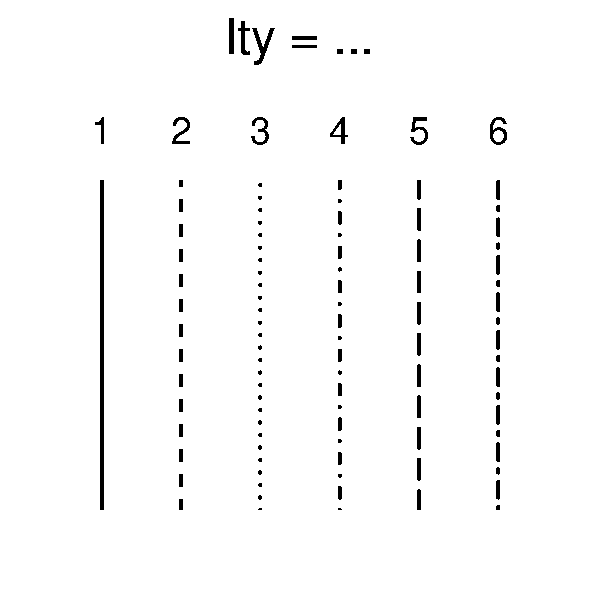
\includegraphics[width=\maxwidth]{figure/unnamed-chunk-207-1} 

\end{knitrout}
\end{tiny}
\label{fig:ltytypes}
\caption{Line types generated from arguments to lty.}
\end{marginfigure}


\vspace{5mm} %5mm vertical space
\noindent
\setlength{\fboxrule}{1.5pt}
\fbox{
\parbox{\textwidth}{

\newfun{abline()}\index{abline()}

\hline

\begin{description}

\item[\tt{a, b}] \hfill \\
Numeric scalars or vectors indicating the slope (\texttt{a}) and intercept {\texttt{b}} of the line(s)

\item[\tt{h, v}] \hfill \\
Numeric scalars or vectors indicating the y-value of horizontal lines (\texttt{h}) or x-values of vertical lines {\texttt{v}}. For example, \texttt{abline(h = 1)} will add a horizontal line at y = 1, while \texttt{abline(v = 10)} will add a vertical line at x = 1

\item[\tt{lty, lwd}] \hfill \\
Type (\texttt{lty}) and width (\texttt{lwd}) of line. See margin Figure~\ref{fig:ltytypes} to see line types.

\end{description}

}
}
\vspace{5mm} %5mm vertical space


For example, to add a vertical line at an x-value of 0 or a horizontal line at a y-vale at 100 you'd enter

\begin{knitrout}
\definecolor{shadecolor}{rgb}{0.969, 0.969, 0.969}\color{fgcolor}\begin{kframe}
\begin{alltt}
\hlkwd{abline}\hlstd{(}\hlkwc{v} \hlstd{=} \hlnum{0}\hlstd{)} \hlcom{# Add a vertical line at x = 0}
\hlkwd{abline}\hlstd{(}\hlkwc{h} \hlstd{=} \hlnum{100}\hlstd{)} \hlcom{# Add a horizontal line at y = 100}
\end{alltt}
\end{kframe}
\end{knitrout}

You can easily use abline() to add gridlines to plots by entering vectors in the \texttt{h} and \texttt{v} arguments. For example, to add gridlines to a plot at x-values and y-values from 0 to 10 in steps of 1, you'd enter

\begin{knitrout}
\definecolor{shadecolor}{rgb}{0.969, 0.969, 0.969}\color{fgcolor}\begin{kframe}
\begin{alltt}
\hlkwd{abline}\hlstd{(}\hlkwc{v} \hlstd{=} \hlnum{1}\hlopt{:}\hlnum{10}\hlstd{)} \hlcom{# Add vertical lines from 1 to 10}
\hlkwd{abline}\hlstd{(}\hlkwc{h} \hlstd{=} \hlnum{1}\hlopt{:}\hlnum{10}\hlstd{)} \hlcom{# Add horizontal lines from 1 to 10}
\end{alltt}
\end{kframe}
\end{knitrout}

In margin Figure~\ref{fig:gridlinesexample} I add gridlines and a diagonal reference line to a plot before adding points.

\begin{marginfigure}
\begin{tiny}
\begin{knitrout}
\definecolor{shadecolor}{rgb}{0.969, 0.969, 0.969}\color{fgcolor}\begin{kframe}
\begin{alltt}
\hlcom{# Create a blank plot}
\hlkwd{plot}\hlstd{(}\hlkwc{x} \hlstd{=} \hlnum{1}\hlstd{,}
     \hlkwc{xlab} \hlstd{=} \hlstr{"Group"}\hlstd{,}
     \hlkwc{ylab} \hlstd{=} \hlstr{"Length"}\hlstd{,}
     \hlkwc{type} \hlstd{=} \hlstr{"n"}\hlstd{,}
     \hlkwc{main} \hlstd{=} \hlstr{"Gridlines with abline()"}\hlstd{,}
     \hlkwc{xlim} \hlstd{=} \hlkwd{c}\hlstd{(}\hlnum{0}\hlstd{,} \hlnum{10}\hlstd{),} \hlkwc{ylim} \hlstd{=} \hlkwd{c}\hlstd{(}\hlnum{0}\hlstd{,} \hlnum{10}\hlstd{))}

\hlcom{# Add horizontal gridlines}
\hlkwd{abline}\hlstd{(}\hlkwc{h} \hlstd{=} \hlnum{1}\hlopt{:}\hlnum{10}\hlstd{,}
       \hlkwc{lwd} \hlstd{=} \hlnum{1}\hlstd{,}
       \hlkwc{col} \hlstd{=} \hlkwd{gray}\hlstd{(}\hlnum{.8}\hlstd{))}

\hlcom{# Add vertical gridlines}
\hlkwd{abline}\hlstd{(}\hlkwc{v} \hlstd{=} \hlnum{1}\hlopt{:}\hlnum{10}\hlstd{,}
       \hlkwc{col} \hlstd{=} \hlkwd{gray}\hlstd{(}\hlnum{.8}\hlstd{))}

\hlcom{# Add main diagonal reference line}
\hlkwd{abline}\hlstd{(}\hlkwc{a} \hlstd{=} \hlnum{0}\hlstd{,}
       \hlkwc{b} \hlstd{=} \hlnum{1}\hlstd{,}
       \hlkwc{lwd} \hlstd{=} \hlnum{2}\hlstd{,}
       \hlkwc{lty} \hlstd{=} \hlnum{2}\hlstd{)}

\hlcom{# Create data}
\hlstd{x.data} \hlkwb{<-} \hlkwd{rnorm}\hlstd{(}\hlnum{100}\hlstd{,} \hlkwc{mean} \hlstd{=} \hlnum{5}\hlstd{,} \hlkwc{sd} \hlstd{=} \hlnum{2}\hlstd{)}
\hlstd{y.data} \hlkwb{<-} \hlstd{x.data} \hlopt{+} \hlkwd{rnorm}\hlstd{(}\hlnum{100}\hlstd{,} \hlkwc{mean} \hlstd{=} \hlnum{0}\hlstd{,} \hlkwc{sd} \hlstd{=} \hlnum{3}\hlstd{)}

\hlcom{# Add points}
\hlkwd{points}\hlstd{(}\hlkwc{x} \hlstd{= x.data,}
       \hlkwc{y} \hlstd{= y.data,} \hlkwc{pch} \hlstd{=} \hlnum{16}\hlstd{,}
       \hlkwc{col} \hlstd{=} \hlkwd{gray}\hlstd{(}\hlnum{.4}\hlstd{,} \hlkwc{alpha} \hlstd{=} \hlnum{.5}\hlstd{),}
       \hlkwc{cex} \hlstd{=} \hlkwd{c}\hlstd{(}\hlkwd{runif}\hlstd{(}\hlnum{90}\hlstd{,} \hlnum{0}\hlstd{,} \hlnum{2}\hlstd{),} \hlkwd{runif}\hlstd{(}\hlnum{10}\hlstd{,} \hlnum{3}\hlstd{,} \hlnum{4}\hlstd{))}
       \hlstd{)}
\end{alltt}
\end{kframe}
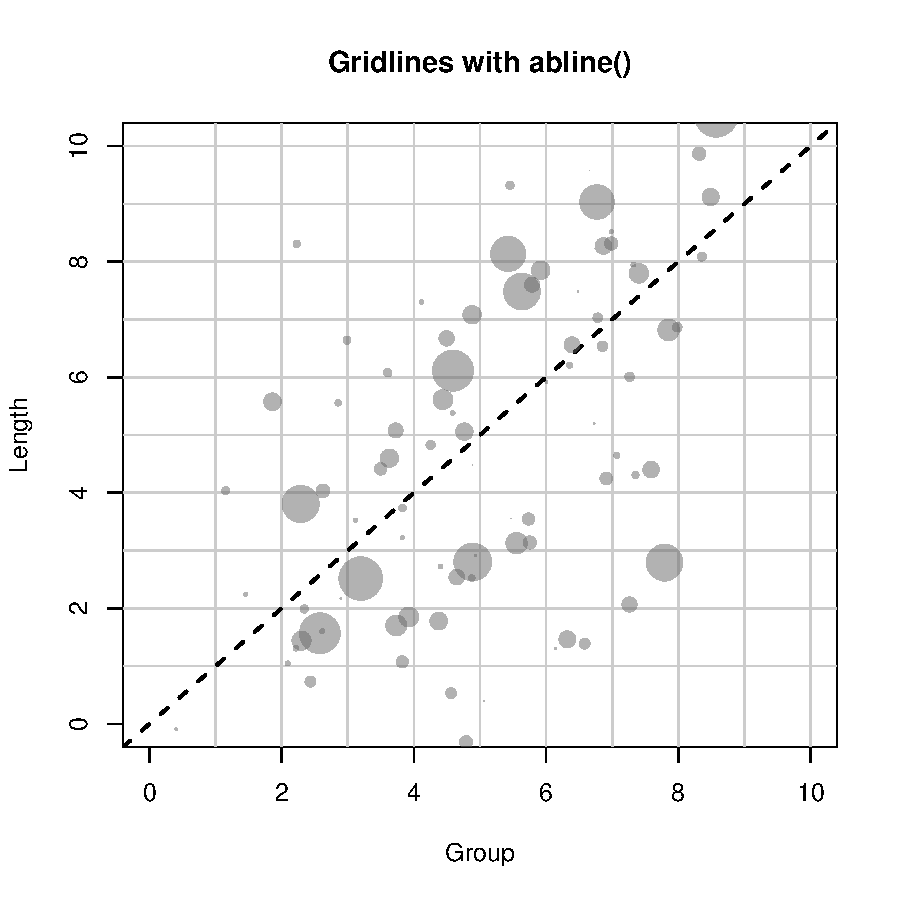
\includegraphics[width=\maxwidth]{figure/unnamed-chunk-210-1} 

\end{knitrout}
\caption{Adding gridlines to a plot with abline().}
\label{fig:gridlinesexample}
\end{tiny}
\end{marginfigure}

Next, we'll move on to \texttt{text}, which adds text to a plot

\subsection{text()}

With \texttt{text()}, you can add text to a plot. You can use text() to highlight specific points of interest in the plot, or to add information (like a third variable) for every point in a plot. Here are the main arguments to \texttt{text()}




\vspace{5mm} %5mm vertical space
\noindent
\setlength{\fboxrule}{1.5pt}
\fbox{
\parbox{\textwidth}{

\newfun{text()}\index{text()}

\hline

\begin{description}

\item[\tt{x, y}] \hfill \\
Numeric scalars or vectors specifying the coordinates of the \textt{labels}

\item[\tt{labels}] \hfill \\
String vector of the text you're plotting. Use the \textt{paste()} function to create multiple strings or combine strings with numeric objects.

\item[\tt{cex}] \hfill \\
Numeric scalar or vector specifying the size of the \texttt{labels}

\item[\tt{adj}] \hfill \\
A numerical value between 0 and 1 specifying the horizontal and/or vertical justification of text. Use 0 for left justification, .5 for centering, and 1 for right justification.

\item[\tt{pos}] \hfill \\
     Specifies the position of the text relative to the x-y coordinates. Values of 1, 2, 3 and 4 respectively indicate below, to the left, above, and to the right of the x-y coordinates.

\item[\tt{font}] \hfill \\
 The font face. 1 = plain, 2 = bold, 3 = italic, 4 = bold-italic.

\end{description}

}
}
\vspace{5mm} %5mm vertical space


For example, if you want to add the text ``This is the center of the plot" to a plot at the coordinates (0, 0), you'd enter

\begin{knitrout}
\definecolor{shadecolor}{rgb}{0.969, 0.969, 0.969}\color{fgcolor}\begin{kframe}
\begin{alltt}
\hlkwd{text}\hlstd{(}\hlkwc{x} \hlstd{=} \hlnum{0}\hlstd{,}
     \hlkwc{y} \hlstd{=} \hlnum{0}\hlstd{,}
     \hlkwc{labels} \hlstd{=} \hlstr{"This is the center of the plot"}\hlstd{)}
\end{alltt}
\end{kframe}
\end{knitrout}

Alternatively, let's say you have a scatterplot and wanted to add the x-values in text right above (pos = 3) each point, you could do this by using the code:

\begin{knitrout}
\definecolor{shadecolor}{rgb}{0.969, 0.969, 0.969}\color{fgcolor}\begin{kframe}
\begin{alltt}
\hlkwd{text}\hlstd{(}\hlkwc{x} \hlstd{= x.data,} \hlcom{# X-values of data}
     \hlkwc{y} \hlstd{= y,data,} \hlcom{# X-values of data}
     \hlkwc{labels} \hlstd{= x.data,} \hlcom{# Add text of the x-values}
     \hlkwc{pos} \hlstd{=} \hlnum{3} \hlcom{# Put the text right above the points}
     \hlstd{)}
\end{alltt}
\end{kframe}
\end{knitrout}

To see \texttt{text()} in action, look at margin Figure \ref{fig:textexample} where I put the x-values of some random data right above their points:

\begin{marginfigure}
\begin{tiny}
\begin{knitrout}
\definecolor{shadecolor}{rgb}{0.969, 0.969, 0.969}\color{fgcolor}\begin{kframe}
\begin{alltt}
\hlcom{# Step 1: Generate Data}

\hlstd{x.data} \hlkwb{<-} \hlkwd{rnorm}\hlstd{(}\hlnum{20}\hlstd{,} \hlkwc{mean} \hlstd{=} \hlnum{0}\hlstd{,} \hlkwc{sd} \hlstd{=} \hlnum{20}\hlstd{)}
\hlstd{y.data} \hlkwb{<-} \hlstd{x.data} \hlopt{+} \hlkwd{rnorm}\hlstd{(}\hlnum{20}\hlstd{,} \hlkwc{mean} \hlstd{=} \hlnum{0}\hlstd{,} \hlkwc{sd} \hlstd{=} \hlnum{20}\hlstd{)}

\hlcom{# Step 2:  Create a blank plot}

\hlkwd{plot}\hlstd{(}\hlkwc{x} \hlstd{=} \hlnum{1}\hlstd{,} \hlkwc{xlab} \hlstd{=} \hlstr{""}\hlstd{,} \hlkwc{ylab} \hlstd{=} \hlstr{""}\hlstd{,}
     \hlkwc{type} \hlstd{=} \hlstr{"n"}\hlstd{,} \hlkwc{main} \hlstd{=} \hlstr{"Adding text with text()"}\hlstd{,}
     \hlkwc{xlim} \hlstd{=} \hlkwd{c}\hlstd{(}\hlopt{-}\hlnum{50}\hlstd{,} \hlnum{50}\hlstd{),} \hlkwc{ylim} \hlstd{=} \hlkwd{c}\hlstd{(}\hlopt{-}\hlnum{50}\hlstd{,} \hlnum{50}\hlstd{))}

\hlcom{# Step 3: Add points}

\hlkwd{points}\hlstd{(}\hlkwc{x} \hlstd{= x.data,} \hlkwc{y} \hlstd{= y.data,}
       \hlkwc{pch} \hlstd{=} \hlnum{16}\hlstd{,} \hlkwc{col} \hlstd{=} \hlkwd{gray}\hlstd{(}\hlnum{.5}\hlstd{,} \hlkwc{alpha} \hlstd{=} \hlnum{.2}\hlstd{))}

\hlcom{# Step #4: Add x-coordinates in text above points}
\hlkwd{text}\hlstd{(}\hlkwc{x} \hlstd{= x.data,}
     \hlkwc{y} \hlstd{= y.data,}
     \hlkwc{labels} \hlstd{=} \hlkwd{round}\hlstd{(x.data,} \hlnum{0}\hlstd{),}
     \hlkwc{pos} \hlstd{=} \hlnum{3}\hlstd{,} \hlcom{# put coordinates below the points}
     \hlkwc{cex} \hlstd{=} \hlnum{.7}
     \hlstd{)}
\end{alltt}
\end{kframe}
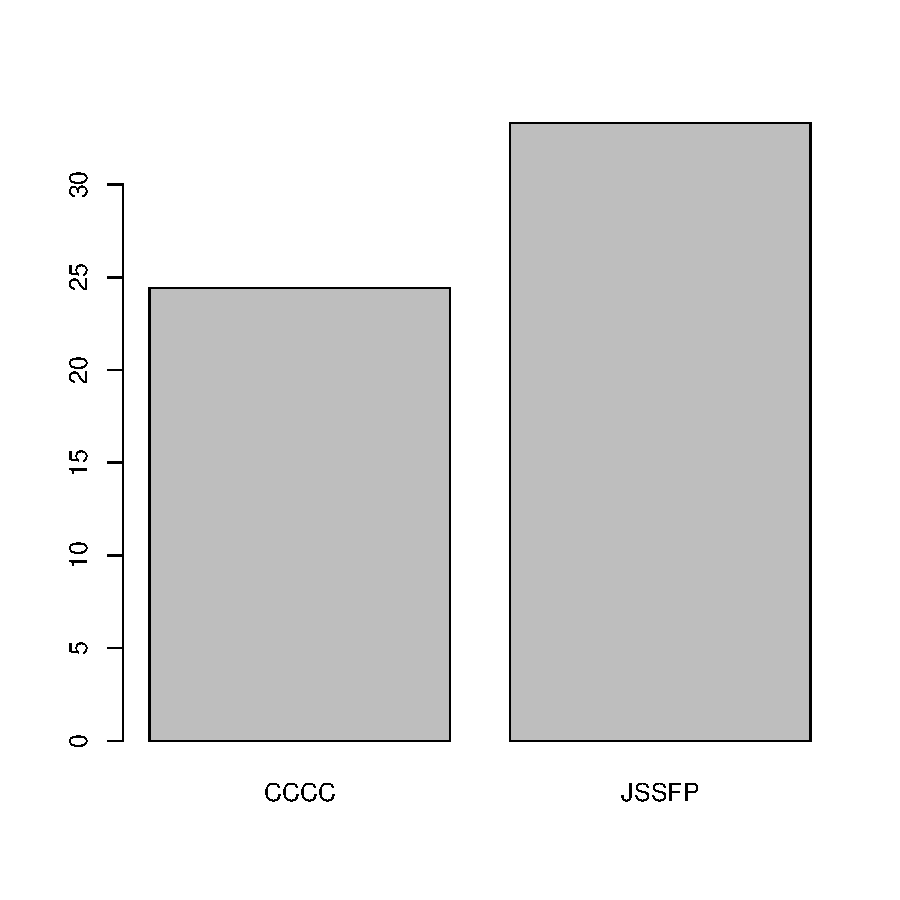
\includegraphics[width=\maxwidth]{figure/unnamed-chunk-213-1} 

\end{knitrout}
\end{tiny}
\caption{Adding text to a plot with text().}
\label{fig:textexample}
\end{marginfigure}

When entering text in the \texttt{labels} argument, keep in mind that R will, by default, plot the entire text in one line. However, if you are adding a long text string (like a sentence), you may want to separate the text into separate lines. To do this, add the text \texttt{"\textbackslash n"} where you want new lines to start. Look at Figure~\ref{fig:manylines} for an example.

\begin{marginfigure} To plot text on separate lines in a plot, put the tag \texttt{"\textbackslash n"} between lines.
\begin{tiny}
\begin{knitrout}
\definecolor{shadecolor}{rgb}{0.969, 0.969, 0.969}\color{fgcolor}\begin{kframe}
\begin{alltt}
\hlkwd{plot}\hlstd{(}\hlnum{1}\hlstd{,} \hlkwc{type} \hlstd{=} \hlstr{"n"}\hlstd{,} \hlkwc{main} \hlstd{=} \hlstr{"The \textbackslash{}\textbackslash{}n tag"}\hlstd{,}
     \hlkwc{xlab} \hlstd{=} \hlstr{""}\hlstd{,} \hlkwc{ylab} \hlstd{=} \hlstr{""}\hlstd{)}

\hlcom{# Text without \textbackslash{}n breaks}
\hlkwd{text}\hlstd{(}\hlkwc{x} \hlstd{=} \hlnum{1}\hlstd{,} \hlkwc{y} \hlstd{=} \hlnum{1.3}\hlstd{,} \hlkwc{labels} \hlstd{=} \hlstr{"Text without \textbackslash{}\textbackslash{}n"}\hlstd{,} \hlkwc{font} \hlstd{=} \hlnum{2}\hlstd{)}
\hlkwd{text}\hlstd{(}\hlkwc{x} \hlstd{=} \hlnum{1}\hlstd{,} \hlkwc{y} \hlstd{=} \hlnum{1.2}\hlstd{,}
     \hlkwc{labels} \hlstd{=} \hlstr{"Haikus are easy. But sometimes they don't make sense. Refrigerator"}
     \hlstd{)}
\hlkwd{abline}\hlstd{(}\hlkwc{h} \hlstd{=} \hlnum{1}\hlstd{,} \hlkwc{lty} \hlstd{=} \hlnum{2}\hlstd{)}
\hlcom{# Text with \textbackslash{}n breaks}
\hlkwd{text}\hlstd{(}\hlkwc{x} \hlstd{=} \hlnum{1}\hlstd{,} \hlkwc{y} \hlstd{=} \hlnum{.92}\hlstd{,} \hlkwc{labels} \hlstd{=} \hlstr{"Text with \textbackslash{}\textbackslash{}n"}\hlstd{,} \hlkwc{font} \hlstd{=} \hlnum{2}\hlstd{)}
\hlkwd{text}\hlstd{(}\hlkwc{x} \hlstd{=} \hlnum{1}\hlstd{,} \hlkwc{y} \hlstd{=} \hlnum{.7}\hlstd{,}
     \hlkwc{labels} \hlstd{=} \hlstr{"Haikus are easy\textbackslash{}nBut sometimes they don't make sense\textbackslash{}nRefrigerator"}
     \hlstd{)}
\end{alltt}
\end{kframe}
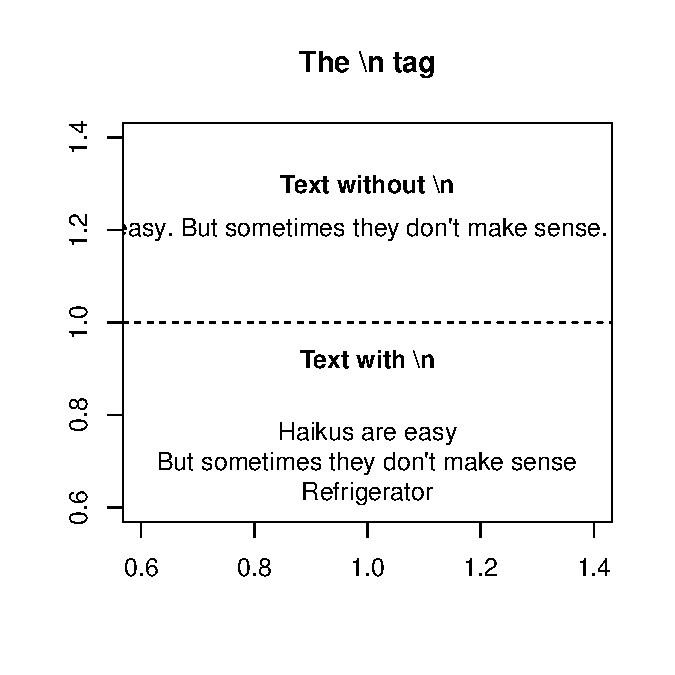
\includegraphics[width=\maxwidth]{figure/unnamed-chunk-214-1} 

\end{knitrout}
\end{tiny}
\label{fig:manylines}
\caption{Using the \texttt{"\textbackslash n"} tag to plot text on separate lines.}
\end{marginfigure}


\subsection{Formatting text for plotting}

A common way to use text in a plot, either in the main title of a plot or using the \texttt{text()} function, is to combine text with numerical data. For example, you may want to include the text "Mean = 3.14" in a plot to show that the mean of the data is 3.14. But how can we combine numerical data with text? In R, we can do this with the \texttt{paste()} function:




\vspace{5mm} %5mm vertical space
\noindent
\setlength{\fboxrule}{1.5pt}
\fbox{
\parbox{\textwidth}{

\newfun{paste()}\index{paste()}

\hline

\begin{description}

\item[\tt{...}] \hfill \\
One or more scalars or vectors (numeric or string) to be combined. For example \texttt{paste("The mean of x is ", mean(x), sep = "")} will create a string combining text and a statistic calculated from data.

\item[\tt{sep}] \hfill \\
A character string that separates the arguments. Set to \texttt{""} for no separation

\end{description}

}
}
\vspace{5mm} %5mm vertical space



The paste function will be helpful to you anytime you want to combine either multiple strings, or text and strings together. For example, let's say you want to write text in a plot that says \texttt{The mean of these data are XXX}, where XXX is replaced by the group mean. To do this, just include the main text and the object referring to the numerical mean as arguments to \texttt{paste()}:\marginnote{When you include descriptive statistics in a plot, you will almost always want to use the \texttt{round(x, digits)} function to reduce the number of digits in the statistic.}

\begin{footnotesize}
\begin{knitrout}
\definecolor{shadecolor}{rgb}{0.969, 0.969, 0.969}\color{fgcolor}\begin{kframe}
\begin{alltt}
\hlstd{data} \hlkwb{<-} \hlkwd{rnorm}\hlstd{(}\hlnum{200}\hlstd{,} \hlkwc{mean} \hlstd{=} \hlnum{20}\hlstd{,} \hlkwc{sd} \hlstd{=} \hlnum{10}\hlstd{)}
\hlkwd{mean}\hlstd{(data)}
\end{alltt}
\begin{verbatim}
## [1] 21.21807
\end{verbatim}
\begin{alltt}
\hlkwd{paste}\hlstd{(}\hlstr{"The mean of the group is"}\hlstd{,} \hlkwd{mean}\hlstd{(data))} \hlcom{# No rounding}
\end{alltt}
\begin{verbatim}
## [1] "The mean of the group is 21.218069485714"
\end{verbatim}
\begin{alltt}
\hlkwd{paste}\hlstd{(}\hlstr{"The mean of the group is"}\hlstd{,} \hlkwd{round}\hlstd{(}\hlkwd{mean}\hlstd{(data),} \hlnum{2}\hlstd{))} \hlcom{# No rounding}
\end{alltt}
\begin{verbatim}
## [1] "The mean of the group is 21.22"
\end{verbatim}
\end{kframe}
\end{knitrout}
\end{footnotesize}

\end{marginnote}

You can also use vectors as arguments to the \texttt{paste()} function. For example, let's say that you want to create a vector of labels for 5 groups, and you want each group to be labelled \texttt{"Group X"}. We can easily do this with \texttt{paste()}

\begin{footnotesize}
\begin{knitrout}
\definecolor{shadecolor}{rgb}{0.969, 0.969, 0.969}\color{fgcolor}\begin{kframe}
\begin{alltt}
\hlkwd{paste}\hlstd{(}\hlstr{"Group"}\hlstd{,} \hlnum{1}\hlopt{:}\hlnum{5}\hlstd{,} \hlkwc{sep} \hlstd{=} \hlstr{" "}\hlstd{)}
\end{alltt}
\begin{verbatim}
## [1] "Group 1" "Group 2" "Group 3" "Group 4" "Group 5"
\end{verbatim}
\end{kframe}
\end{knitrout}
\end{footnotesize}

\pagebreak
\subsection{curve()}

\begin{marginfigure}
\begin{tiny}
\begin{knitrout}
\definecolor{shadecolor}{rgb}{0.969, 0.969, 0.969}\color{fgcolor}\begin{kframe}
\begin{alltt}
\hlkwd{plot}\hlstd{(}\hlnum{1}\hlstd{,} \hlkwc{xlim} \hlstd{=} \hlkwd{c}\hlstd{(}\hlopt{-}\hlnum{5}\hlstd{,} \hlnum{5}\hlstd{),} \hlkwc{ylim} \hlstd{=} \hlkwd{c}\hlstd{(}\hlopt{-}\hlnum{5}\hlstd{,} \hlnum{5}\hlstd{),}
     \hlkwc{type} \hlstd{=} \hlstr{"n"}\hlstd{,} \hlkwc{main} \hlstd{=} \hlstr{"Plotting function lines with curve()"}\hlstd{,}
     \hlkwc{ylab} \hlstd{=} \hlstr{""}\hlstd{,} \hlkwc{xlab} \hlstd{=} \hlstr{""}\hlstd{)}
\hlkwd{abline}\hlstd{(}\hlkwc{h} \hlstd{=} \hlnum{0}\hlstd{)}
\hlkwd{abline}\hlstd{(}\hlkwc{v} \hlstd{=} \hlnum{0}\hlstd{)}

\hlkwd{require}\hlstd{(}\hlstr{"RColorBrewer"}\hlstd{)}
\hlstd{col.vec} \hlkwb{<-} \hlkwd{brewer.pal}\hlstd{(}\hlnum{12}\hlstd{,} \hlkwc{name} \hlstd{=} \hlstr{"Set3"}\hlstd{)[}\hlnum{4}\hlopt{:}\hlnum{7}\hlstd{]}

\hlkwd{curve}\hlstd{(}\hlkwc{expr} \hlstd{= x}\hlopt{^}\hlnum{2}\hlstd{,} \hlkwc{from} \hlstd{=} \hlopt{-}\hlnum{5}\hlstd{,} \hlkwc{to} \hlstd{=} \hlnum{5}\hlstd{,}
      \hlkwc{add} \hlstd{= T,} \hlkwc{lwd} \hlstd{=} \hlnum{2}\hlstd{,} \hlkwc{col} \hlstd{= col.vec[}\hlnum{1}\hlstd{])}
\hlkwd{curve}\hlstd{(}\hlkwc{expr} \hlstd{= x}\hlopt{^}\hlnum{.5}\hlstd{,} \hlkwc{from} \hlstd{=} \hlnum{0}\hlstd{,} \hlkwc{to} \hlstd{=} \hlnum{5}\hlstd{,}
      \hlkwc{add} \hlstd{= T,} \hlkwc{lwd} \hlstd{=} \hlnum{2}\hlstd{,} \hlkwc{col} \hlstd{= col.vec[}\hlnum{2}\hlstd{])}
\hlkwd{curve}\hlstd{(}\hlkwc{expr} \hlstd{= sin,} \hlkwc{from} \hlstd{=} \hlopt{-}\hlnum{5}\hlstd{,} \hlkwc{to} \hlstd{=} \hlnum{5}\hlstd{,}
      \hlkwc{add} \hlstd{= T,} \hlkwc{lwd} \hlstd{=} \hlnum{2}\hlstd{,} \hlkwc{col} \hlstd{= col.vec[}\hlnum{3}\hlstd{])}

\hlstd{my.fun} \hlkwb{<-} \hlkwa{function}\hlstd{(}\hlkwc{x}\hlstd{) \{}\hlkwd{return}\hlstd{(}\hlkwd{dnorm}\hlstd{(x,} \hlkwc{mean} \hlstd{=} \hlnum{2}\hlstd{,} \hlkwc{sd} \hlstd{=} \hlnum{.2}\hlstd{))\}}
\hlkwd{curve}\hlstd{(}\hlkwc{expr} \hlstd{= my.fun,} \hlkwc{from} \hlstd{=} \hlopt{-}\hlnum{5}\hlstd{,} \hlkwc{to} \hlstd{=} \hlnum{5}\hlstd{,}
      \hlkwc{add} \hlstd{= T,} \hlkwc{lwd} \hlstd{=} \hlnum{2}\hlstd{,} \hlkwc{col} \hlstd{= col.vec[}\hlnum{4}\hlstd{])}

\hlkwd{legend}\hlstd{(}\hlstr{"bottomright"}\hlstd{,}
       \hlkwc{legend} \hlstd{=} \hlkwd{c}\hlstd{(}\hlstr{"x^2"}\hlstd{,} \hlstr{"x^.5"}\hlstd{,} \hlstr{"sin(x)"}\hlstd{,} \hlstr{"dnorm(x, 2, .2"}\hlstd{),}
       \hlkwc{col} \hlstd{= col.vec[}\hlnum{1}\hlopt{:}\hlnum{4}\hlstd{],} \hlkwc{lwd} \hlstd{=} \hlnum{2}\hlstd{,}
       \hlkwc{lty} \hlstd{=} \hlnum{1}\hlstd{,} \hlkwc{cex} \hlstd{=} \hlnum{.8}\hlstd{,} \hlkwc{bty} \hlstd{=} \hlstr{"n"}
       \hlstd{)}
\end{alltt}
\end{kframe}
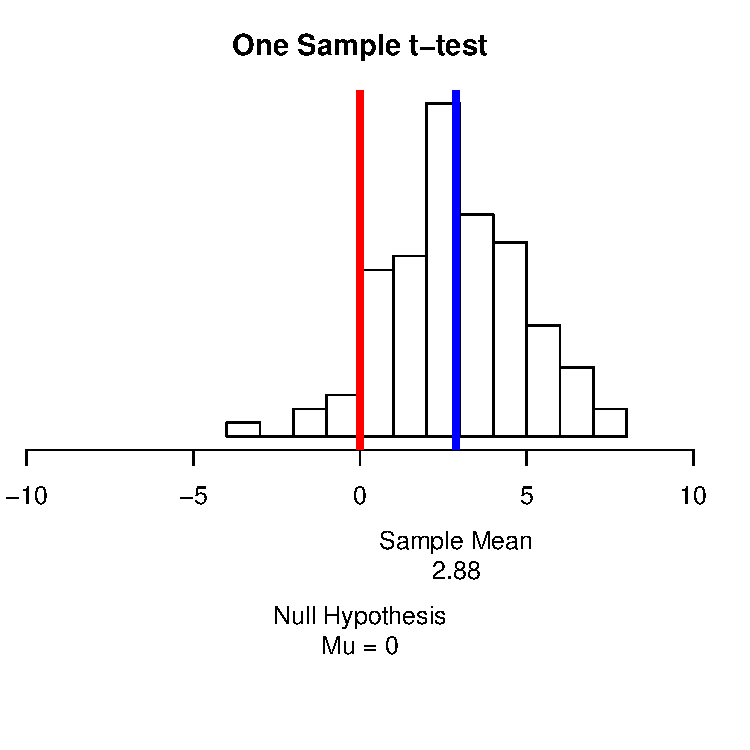
\includegraphics[width=\maxwidth]{figure/unnamed-chunk-217-1} 

\end{knitrout}
\end{tiny}
\caption{Using \texttt{curve()} to easily create lines of functions}
\label{fig:functionlines}
\end{marginfigure}


The \texttt{curve()} function allows you to add a line showing a specific function or equation to a plot


\vspace{5mm} %5mm vertical space
\noindent
\setlength{\fboxrule}{1.5pt}
\fbox{
\parbox{\textwidth}{

\newfun{curve()}\index{curve()}

\hline

\begin{description}

\item[\tt{expr}] \hfill \\
 The name of a function written as a function of \texttt{x} that returns a single vector. You can either use base functions in R like \texttt{expr = $x^2$}, \texttt{expr = x + 4 - 2}, or use your own custom functions such as \texttt{expr = my.fun}, where \texttt{my.fun} is previously defined (e.g.; \texttt{my.fun <- function(x) {dnorm(x, mean = 10, sd = 3)}})

\item[\tt{from, to}] \hfill \\
 The starting (\texttt{from}) and ending (\texttt{to}) value of x to be plotted.

\item[\tt{add}] \hfill \\
 A logical value indicating whether or not to add the curve to an existing plot. If \texttt{add = FALSE}, then \texttt{curve()} will act like a high-level plotting function and create a new plot. If \texttt{add = TRUE}, then \texttt{curve()} will act like a low-level plotting function.

\item[\tt{lty, lwd, col}] \hfill \\
Additional arguments such as \texttt{lty}, \texttt{col}, \texttt{lwd}, ...

\end{description}

}
}
\vspace{5mm} %5mm vertical space

For example, to add the function $x^2$ to a plot from the x-values -10 to 10, you can run the code:

\begin{knitrout}
\definecolor{shadecolor}{rgb}{0.969, 0.969, 0.969}\color{fgcolor}\begin{kframe}
\begin{alltt}
\hlkwd{curve}\hlstd{(}\hlkwc{expr} \hlstd{= x}\hlopt{^}\hlnum{2}\hlstd{,} \hlkwc{from} \hlstd{=} \hlopt{-}\hlnum{10}\hlstd{,} \hlkwc{to} \hlstd{=} \hlnum{10}\hlstd{)}
\end{alltt}
\end{kframe}
\end{knitrout}

If you want to add a custom function to a plot, you can define the function and then use that function name as the argument to \texttt{expr}. For example, to plot the normal distribution with a mean of 10 and standard deviation of 3, you can use this code:

\begin{knitrout}
\definecolor{shadecolor}{rgb}{0.969, 0.969, 0.969}\color{fgcolor}\begin{kframe}
\begin{alltt}
my.fun <- \hlkwd{function}(x) \{\hlkwd{dnorm}(x, mean = 10, sd = 3)\}
\hlkwd{curve}(expr = my.fun, from = -10, to 10)
\end{alltt}
\end{kframe}
\end{knitrout}


In Figure~\ref{fig:functionlines}, I use the \texttt{curve()} function to create curves of several mathematical formulas.


\pagebreak
\subsection{legend()}


\begin{marginfigure}
\begin{tiny}
\begin{knitrout}
\definecolor{shadecolor}{rgb}{0.969, 0.969, 0.969}\color{fgcolor}\begin{kframe}
\begin{alltt}
\hlcom{# Generate some random data}
\hlstd{female.x} \hlkwb{<-} \hlkwd{rnorm}\hlstd{(}\hlnum{100}\hlstd{)}
\hlstd{female.y} \hlkwb{<-} \hlstd{female.x} \hlopt{+} \hlkwd{rnorm}\hlstd{(}\hlnum{100}\hlstd{)}
\hlstd{male.x} \hlkwb{<-} \hlkwd{rnorm}\hlstd{(}\hlnum{100}\hlstd{)}
\hlstd{male.y} \hlkwb{<-} \hlstd{male.x} \hlopt{+} \hlkwd{rnorm}\hlstd{(}\hlnum{100}\hlstd{)}

\hlcom{# Create plot with data from females}
\hlkwd{plot}\hlstd{(female.x, female.y,} \hlkwc{pch} \hlstd{=} \hlnum{16}\hlstd{,} \hlkwc{col} \hlstd{=} \hlstr{'blue'}\hlstd{,}
     \hlkwc{xlab} \hlstd{=} \hlstr{"x"}\hlstd{,} \hlkwc{ylab} \hlstd{=} \hlstr{"y"}\hlstd{,} \hlkwc{main} \hlstd{=} \hlstr{"Adding a legend with legend()"}
     \hlstd{)}

\hlcom{# Add data from males}
\hlkwd{points}\hlstd{(male.x, male.y,} \hlkwc{pch} \hlstd{=} \hlnum{16}\hlstd{,} \hlkwc{col} \hlstd{=} \hlstr{'orange'}\hlstd{)}

\hlcom{# Add legend}
\hlkwd{legend}\hlstd{(}\hlstr{"bottomright"}\hlstd{,}
       \hlkwc{legend} \hlstd{=} \hlkwd{c}\hlstd{(}\hlstr{"Females"}\hlstd{,} \hlstr{"Males"}\hlstd{),}
       \hlkwc{col} \hlstd{=} \hlkwd{c}\hlstd{(}\hlstr{'blue'}\hlstd{,} \hlstr{'orange'}\hlstd{),}
       \hlkwc{pch} \hlstd{=} \hlkwd{c}\hlstd{(}\hlnum{16}\hlstd{,} \hlnum{16}\hlstd{),}
       \hlkwc{bg} \hlstd{=} \hlstr{"white"}
       \hlstd{)}
\end{alltt}
\end{kframe}
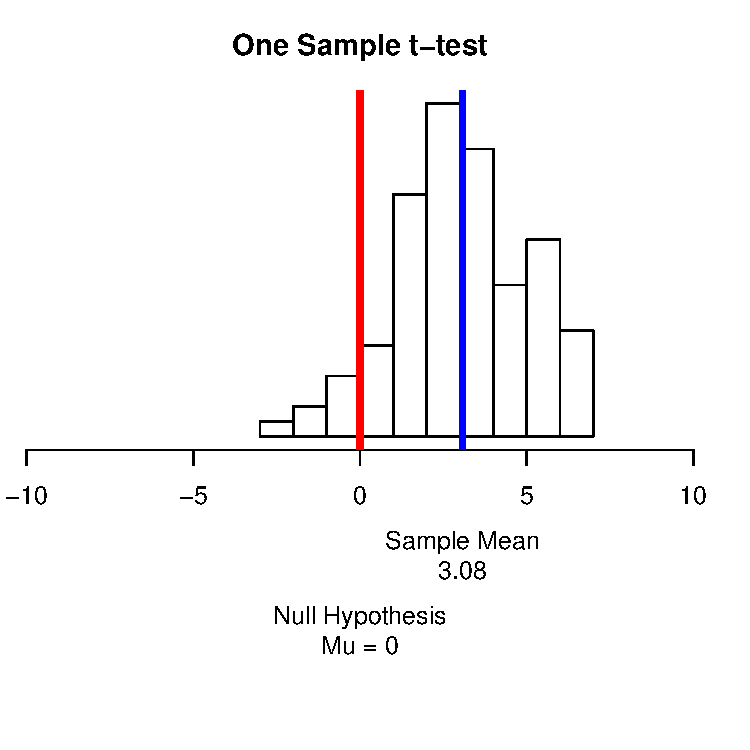
\includegraphics[width=\maxwidth]{figure/unnamed-chunk-220-1} 

\end{knitrout}
\end{tiny}
\label{fig:legendexample}
\caption{Creating a legend labeling the symbol types from different groups}
\end{marginfigure}

The last low-level plotting function that we'll go over in detail is \texttt{legend()} which adds a legend to a plot. This function has the following arguments


\vspace{5mm} %5mm vertical space
\noindent
\setlength{\fboxrule}{1.5pt}
\fbox{
\parbox{\textwidth}{

\newfun{legend()}\index{legend()}

\hline

\begin{description}

\item[\tt{x, y}] \hfill \\
Coordinates of the legend - for example, \texttt{x = 0, y = 0} will put the text at the coordinates (0, 0). Alternatively, you can enter a string indicating where to put the legend (i.e.; "topright", "topleft"). For example, \texttt{"bottomright"} will always put the legend at the bottom right corner of the plot.

\item[\tt{labels}] \hfill \\
  A string vector specifying the text in the legend. For example, \texttt{legend = c("Males, "Females")} will create two groups with names Males and Females.

\item[\tt{pch, lty, lwd, col, pt.bg, ...}] \hfill \\
Additional arguments specifying symbol types (\texttt{pch}), line types (\texttt{lty}), line widths (\texttt{lwd}), background color of symbol types 21 through 25 ((\texttt{pt.bg})) and several other optional arguments. See \texttt{?legend} for a complete list


\end{description}

}
}
\vspace{5mm} %5mm vertical space


For example, to add a legend to to bottom-right of an existing graph where data from females are plotted in blue circles and data from males are plotted in pink circles, you'd use the following code:

\begin{knitrout}
\definecolor{shadecolor}{rgb}{0.969, 0.969, 0.969}\color{fgcolor}\begin{kframe}
\begin{alltt}
\hlkwd{legend}\hlstd{(}\hlstr{"bottomright"}\hlstd{,} \hlcom{# Put legend in bottom right of graph}
       \hlkwc{legend} \hlstd{=} \hlkwd{c}\hlstd{(}\hlstr{"Females"}\hlstd{,} \hlstr{"Males"}\hlstd{),} \hlcom{# Names of groups}
       \hlkwc{col} \hlstd{=} \hlkwd{c}\hlstd{(}\hlstr{"blue"}\hlstd{,} \hlstr{"orange"}\hlstd{),} \hlcom{# Colors of symbols}
       \hlkwc{pch} \hlstd{=} \hlkwd{c}\hlstd{(}\hlnum{16}\hlstd{,} \hlnum{16}\hlstd{)} \hlcom{# Point types}
       \hlstd{)}
\end{alltt}
\end{kframe}
\end{knitrout}

In margin Figure~\ref{fig:legendexample} I use this code to add a legend to plot containing data from males and females.


\pagebreak
\section{Additional low-level plotting functions}

There are many more low-level plotting functions that can add additional elements to your plots. Here are some I use. To see examples of how to use each one, check out their associated help menus.



\begin{marginfigure}
\begin{tiny}
\begin{knitrout}
\definecolor{shadecolor}{rgb}{0.969, 0.969, 0.969}\color{fgcolor}\begin{kframe}
\begin{alltt}
\hlkwd{par}\hlstd{(}\hlkwc{mar} \hlstd{=} \hlkwd{c}\hlstd{(}\hlnum{0}\hlstd{,} \hlnum{0}\hlstd{,} \hlnum{3}\hlstd{,} \hlnum{0}\hlstd{))}

\hlkwd{plot}\hlstd{(}\hlnum{1}\hlstd{,} \hlkwc{xlim} \hlstd{=} \hlkwd{c}\hlstd{(}\hlnum{1}\hlstd{,} \hlnum{100}\hlstd{),} \hlkwc{ylim} \hlstd{=} \hlkwd{c}\hlstd{(}\hlnum{1}\hlstd{,} \hlnum{100}\hlstd{),}
     \hlkwc{type} \hlstd{=} \hlstr{"n"}\hlstd{,} \hlkwc{xaxt} \hlstd{=} \hlstr{"n"}\hlstd{,} \hlkwc{yaxt} \hlstd{=} \hlstr{"n"}\hlstd{,}
     \hlkwc{ylab} \hlstd{=} \hlstr{""}\hlstd{,} \hlkwc{xlab} \hlstd{=} \hlstr{""}\hlstd{,} \hlkwc{main} \hlstd{=} \hlstr{"Adding simple figures to a plot"}\hlstd{)}

\hlkwd{text}\hlstd{(}\hlnum{25}\hlstd{,} \hlnum{95}\hlstd{,} \hlkwc{labels} \hlstd{=} \hlstr{"rect()"}\hlstd{)}

\hlkwd{rect}\hlstd{(}\hlkwc{xleft} \hlstd{=} \hlnum{10}\hlstd{,} \hlkwc{ybottom} \hlstd{=} \hlnum{70}\hlstd{,}
     \hlkwc{xright} \hlstd{=} \hlnum{40}\hlstd{,} \hlkwc{ytop} \hlstd{=} \hlnum{90}\hlstd{,} \hlkwc{lwd} \hlstd{=} \hlnum{2}\hlstd{,} \hlkwc{col} \hlstd{=} \hlstr{"coral"}\hlstd{)}

\hlkwd{text}\hlstd{(}\hlnum{25}\hlstd{,} \hlnum{60}\hlstd{,} \hlkwc{labels} \hlstd{=} \hlstr{"polygon()"}\hlstd{)}

\hlkwd{polygon}\hlstd{(}\hlkwc{x} \hlstd{=} \hlkwd{runif}\hlstd{(}\hlnum{6}\hlstd{,} \hlnum{15}\hlstd{,} \hlnum{35}\hlstd{),}
        \hlkwc{y} \hlstd{=} \hlkwd{runif}\hlstd{(}\hlnum{6}\hlstd{,} \hlnum{40}\hlstd{,} \hlnum{55}\hlstd{),}
        \hlkwc{col} \hlstd{=} \hlstr{"skyblue"}
        \hlstd{)}


\hlcom{# polygon(x = c(15, 35, 25, 15),}
\hlcom{#         y = c(40, 40, 55, 40),}
\hlcom{#         col = "skyblue"}
\hlcom{#         )}

\hlkwd{text}\hlstd{(}\hlnum{25}\hlstd{,} \hlnum{30}\hlstd{,} \hlkwc{labels} \hlstd{=} \hlstr{"segments()"}\hlstd{)}

\hlkwd{segments}\hlstd{(}\hlkwc{x0} \hlstd{=} \hlkwd{runif}\hlstd{(}\hlnum{5}\hlstd{,} \hlnum{10}\hlstd{,} \hlnum{40}\hlstd{),}
         \hlkwc{y0} \hlstd{=} \hlkwd{runif}\hlstd{(}\hlnum{5}\hlstd{,} \hlnum{5}\hlstd{,} \hlnum{25}\hlstd{),}
         \hlkwc{x1} \hlstd{=} \hlkwd{runif}\hlstd{(}\hlnum{5}\hlstd{,} \hlnum{10}\hlstd{,} \hlnum{40}\hlstd{),}
         \hlkwc{y1} \hlstd{=} \hlkwd{runif}\hlstd{(}\hlnum{5}\hlstd{,} \hlnum{5}\hlstd{,} \hlnum{25}\hlstd{),} \hlkwc{lwd} \hlstd{=} \hlnum{2}
         \hlstd{)}

\hlkwd{text}\hlstd{(}\hlnum{75}\hlstd{,} \hlnum{95}\hlstd{,} \hlkwc{labels} \hlstd{=} \hlstr{"symbols(circles)"}\hlstd{)}

\hlkwd{symbols}\hlstd{(}\hlkwc{x} \hlstd{=} \hlkwd{runif}\hlstd{(}\hlnum{3}\hlstd{,} \hlnum{60}\hlstd{,} \hlnum{90}\hlstd{),}
        \hlkwc{y} \hlstd{=} \hlkwd{runif}\hlstd{(}\hlnum{3}\hlstd{,} \hlnum{60}\hlstd{,} \hlnum{70}\hlstd{),}
        \hlkwc{circles} \hlstd{=} \hlkwd{c}\hlstd{(}\hlnum{1}\hlstd{,} \hlnum{.1}\hlstd{,} \hlnum{.3}\hlstd{),}
        \hlkwc{add} \hlstd{= T,} \hlkwc{bg} \hlstd{=} \hlkwd{gray}\hlstd{(}\hlnum{.5}\hlstd{,} \hlnum{.1}\hlstd{))}

\hlkwd{text}\hlstd{(}\hlnum{75}\hlstd{,} \hlnum{30}\hlstd{,} \hlkwc{labels} \hlstd{=} \hlstr{"arrows()"}\hlstd{)}

\hlkwd{arrows}\hlstd{(}\hlkwc{x0} \hlstd{=} \hlkwd{runif}\hlstd{(}\hlnum{3}\hlstd{,} \hlnum{60}\hlstd{,} \hlnum{90}\hlstd{),}
         \hlkwc{y0} \hlstd{=} \hlkwd{runif}\hlstd{(}\hlnum{3}\hlstd{,} \hlnum{10}\hlstd{,} \hlnum{25}\hlstd{),}
         \hlkwc{x1} \hlstd{=} \hlkwd{runif}\hlstd{(}\hlnum{3}\hlstd{,} \hlnum{60}\hlstd{,} \hlnum{90}\hlstd{),}
         \hlkwc{y1} \hlstd{=} \hlkwd{runif}\hlstd{(}\hlnum{3}\hlstd{,} \hlnum{10}\hlstd{,} \hlnum{25}\hlstd{),}
         \hlkwc{length} \hlstd{=} \hlnum{.1}\hlstd{,} \hlkwc{lwd} \hlstd{=} \hlnum{2}
         \hlstd{)}
\end{alltt}
\end{kframe}
\includegraphics[width=\maxwidth]{figure/unnamed-chunk-222-1} 

\end{knitrout}
\end{tiny}
\end{marginfigure}


\vspace{5mm} %5mm vertical space
\noindent
\setlength{\fboxrule}{1.5pt}
\fbox{
\parbox{\textwidth}{

\newfun{Additional low-level plotting functions}

\hline

\begin{description}

\item[\tt{rect()}] \hfill \\
    Add rectangles to a plot at coordinates specified by \texttt{xleft, ybottom, xright, ybottom}. For example, to add a rectangle with corners at (0, 0) and c(10, 10), specify \texttt{xleft = 0, ybottom = 0, xright = 10, ytop = 10}. Additional arguments like \texttt{col, border} change the color of the rectangle.

\item[\tt{polygon()}] \hfill \\
    Add a polygon to a plot at coordinates specified by vectors x and y. Additional arguments such as \texttt{col, border} change the color of the inside and border of the polygon

\item[\tt{segments(), arrows()}] \hfill \\
 Add segments (lines with fixed endings), or arrows to a plot.

\item[\tt{symbols(add = T)}] \hfill \\
Add symbols (circles, squares, rectangles, stars, thermometers) to a plot. The dimensions of each symbol are specified with specific input types. See \texttt{?symbols} for details. Specify \texttt{add = T} to add to an existing plot or \texttt{add = F} to create a new plot.

\item[\tt{axis()}] \hfill \\
 Add an additional axis to a plot (or add fully customizable  x and y axes). Usually you only use this if you set \texttt{xaxt = "n", yaxt = "n"} in the original high-level plotting function.

\item [\tt{mtext()}] \hfill \\
 Add text to the margins of a plot. Look at the help menu for \texttt{mtext()} to see parameters for this function.
\end{description}

}
}
\vspace{5mm} %5mm vertical space




\section{Saving plots to a file}

Once you've created a plot in R, you may wish to save it to a file so you can use it in another document. To do this, you'll use either the \texttt{pdf()} or \texttt{jpeg()} functions. These functions will save your plot to either a .pdf of jpeg file.


\vspace{5mm} %5mm vertical space
\noindent
\setlength{\fboxrule}{1.5pt}
\fbox{
\parbox{\textwidth}{

\newfun{pdf() and jpeg()}

\hline

\begin{description}

\item[\tt{file}] \hfill \\
    The name and file destination of the final plot entered as a string. For example, to put a plot on my desktop, I'd write \texttt{file = "/Users/Nathaniel/Desktop/plot.pdf"} when creating a pdf, and \texttt{file = "/Users/Nathaniel/Desktop/plot.jpg"} when creating a jpeg.

\item[\tt{width, height}] \hfill \\
    The width and height of the final plot in inches.

\item[\tt{family()}] \hfill \\
An optional name of the font family to use for the plot. For example, \texttt{family = "Helvetica"} will use the Helvetica font for all text (assuming you have Helvetica on your system). For more help on using different fonts, look at section "Using extra fonts in R" in Chapter XX

\item[\tt{dev.off()}] \hfill \\
This is \textit{not} an argument to \texttt{pdf()} and \texttt{jpeg()}. You just need to execute this code after creating the plot to finish creating the image file (see examples below).

\end{description}

}
}
\vspace{5mm} %5mm vertical space

To use these functions to save files, you need to follow 3 steps

\begin{enumerate}
  \item Execute the \texttt{pdf()} or \texttt{jpeg()} functions with \texttt{file, width} and \textt{height} arguments.
  \item Execute all your plotting code.
  \item Complete the file by executing the command \texttt{dev.off()}. This tells R that you're done creating the file.
\end{enumerate}

Here's an example of the three steps.


\begin{knitrout}
\definecolor{shadecolor}{rgb}{0.969, 0.969, 0.969}\color{fgcolor}\begin{kframe}
\begin{alltt}
\hlcom{# Step 1: Call the pdf command}
\hlkwd{pdf}\hlstd{(}\hlkwc{file} \hlstd{=} \hlstr{"/Users/Nathaniel/Desktop/My Plot.pdf"}\hlstd{,}   \hlcom{# The directory you want to save the file in}
    \hlkwc{width} \hlstd{=} \hlnum{4}\hlstd{,} \hlcom{# The width of the plot in inches}
    \hlkwc{height} \hlstd{=} \hlnum{4} \hlcom{# The height of the plot in inches}
    \hlstd{)}

\hlcom{# Step 2: Create the plot}
\hlkwd{plot}\hlstd{(}\hlnum{1}\hlopt{:}\hlnum{10}\hlstd{,} \hlnum{1}\hlopt{:}\hlnum{10}\hlstd{)}
\hlkwd{abline}\hlstd{(}\hlkwc{v} \hlstd{=} \hlnum{0}\hlstd{)} \hlcom{# Additional low-level plotting commands}
\hlkwd{text}\hlstd{(}\hlkwc{x} \hlstd{=} \hlnum{0}\hlstd{,} \hlkwc{y} \hlstd{=} \hlnum{1}\hlstd{,} \hlkwc{labels} \hlstd{=} \hlstr{"Random text"}\hlstd{)}

\hlcom{# Step 3: Run dev.off() to create the file!}
\hlkwd{dev.off}\hlstd{()}
\end{alltt}
\end{kframe}
\end{knitrout}


You'll notice that after you close the plot with \texttt{dev.off()}, you'll see a message in the prompt like "null device".

Using the command  \texttt{pdf()} will save the file as a pdf. If you use  \texttt{jpeg()}, it will be saved as a jpeg.


\section{A worked example: Creating a plot with automated numeric labels}


Let's use the \texttt{paste()} command to create a histogram with labels indicating the mean, median, min, and mean of the dataset. We'll do this in 5 steps

1. Generate the data and the histogram\\
2. Add text and reference line for the mean\\
3. Add text and reference line for the minimum\\
4. Add text and reference line for the maximum\\
5. Add a subtitle in full sentences with each summary statistic.

\begin{footnotesize}
\begin{knitrout}
\definecolor{shadecolor}{rgb}{0.969, 0.969, 0.969}\color{fgcolor}\begin{kframe}
\begin{alltt}
\hlcom{# Step 1: Generate data and main histogram}
\hlstd{data} \hlkwb{<-} \hlkwd{rnorm}\hlstd{(}\hlnum{100}\hlstd{,} \hlkwc{mean} \hlstd{=} \hlnum{20}\hlstd{,} \hlkwc{sd} \hlstd{=} \hlnum{2}\hlstd{)}

\hlstd{title.text} \hlkwb{<-} \hlkwd{paste}\hlstd{(}
  \hlstr{"Note: There were "}\hlstd{,} \hlkwd{length}\hlstd{(data),} \hlstr{" data points. The mean and median of the data were "}\hlstd{,}
  \hlkwd{round}\hlstd{(}\hlkwd{mean}\hlstd{(data),} \hlnum{2}\hlstd{),} \hlstr{" and "}\hlstd{,} \hlkwd{round}\hlstd{(}\hlkwd{median}\hlstd{(data,} \hlnum{2}\hlstd{)),} \hlstr{".\textbackslash{}nThe minimum and maximum values were "}\hlstd{,}
  \hlkwd{round}\hlstd{(}\hlkwd{min}\hlstd{(data),} \hlnum{2}\hlstd{),} \hlstr{" and "}\hlstd{,} \hlkwd{round}\hlstd{(}\hlkwd{max}\hlstd{(data),} \hlnum{2}\hlstd{),} \hlstr{"."}\hlstd{,} \hlkwc{sep} \hlstd{=} \hlstr{""}\hlstd{)}


\hlkwd{hist}\hlstd{(data,}
     \hlkwc{xlim} \hlstd{=} \hlkwd{c}\hlstd{(}\hlnum{10}\hlstd{,} \hlnum{30}\hlstd{),}
     \hlkwc{ylim} \hlstd{=} \hlkwd{c}\hlstd{(}\hlnum{0}\hlstd{,} \hlnum{40}\hlstd{),}
     \hlkwc{main} \hlstd{= title.text,}
     \hlkwc{cex.main} \hlstd{=} \hlnum{.7}
     \hlstd{)}

\hlcom{# Step 2: Add mean text and line}
\hlkwd{text}\hlstd{(}\hlkwd{mean}\hlstd{(data),} \hlnum{38}\hlstd{,}
     \hlkwc{labels} \hlstd{=} \hlkwd{paste}\hlstd{(}\hlstr{"Mean\textbackslash{}n"}\hlstd{,} \hlkwd{round}\hlstd{(}\hlkwd{mean}\hlstd{(data),} \hlnum{2}\hlstd{),} \hlkwc{sep} \hlstd{=} \hlstr{""}\hlstd{),}
     \hlkwc{adj} \hlstd{=} \hlnum{0}\hlstd{,}
     \hlkwc{pos} \hlstd{=} \hlnum{4}
\hlstd{)}
\hlkwd{abline}\hlstd{(}\hlkwc{v} \hlstd{=} \hlkwd{mean}\hlstd{(data),} \hlkwc{lty} \hlstd{=} \hlnum{2}\hlstd{)}

\hlcom{# Step 3: Add minimum text and line}
\hlkwd{text}\hlstd{(}\hlkwd{min}\hlstd{(data),} \hlnum{25}\hlstd{,}
     \hlkwc{labels} \hlstd{=} \hlkwd{paste}\hlstd{(}\hlstr{"Min\textbackslash{}n"}\hlstd{,} \hlkwd{round}\hlstd{(}\hlkwd{min}\hlstd{(data),} \hlnum{2}\hlstd{),} \hlkwc{sep} \hlstd{=} \hlstr{""}\hlstd{),}
     \hlkwc{adj} \hlstd{=} \hlnum{0}\hlstd{,}
     \hlkwc{pos} \hlstd{=} \hlnum{2}
\hlstd{)}

\hlkwd{abline}\hlstd{(}\hlkwc{v} \hlstd{=} \hlkwd{min}\hlstd{(data),} \hlkwc{lty} \hlstd{=} \hlnum{2}\hlstd{)}

\hlcom{# Step 4: Add maximum text and line}
\hlkwd{text}\hlstd{(}\hlkwd{max}\hlstd{(data),} \hlnum{25}\hlstd{,}
     \hlkwc{labels} \hlstd{=} \hlkwd{paste}\hlstd{(}\hlstr{"Max\textbackslash{}n"}\hlstd{,} \hlkwd{round}\hlstd{(}\hlkwd{min}\hlstd{(data),} \hlnum{2}\hlstd{),} \hlkwc{sep} \hlstd{=} \hlstr{""}\hlstd{),}
     \hlkwc{adj} \hlstd{=} \hlnum{0}\hlstd{,}
     \hlkwc{pos} \hlstd{=} \hlnum{4}
\hlstd{)}

\hlkwd{abline}\hlstd{(}\hlkwc{v} \hlstd{=} \hlkwd{max}\hlstd{(data),} \hlkwc{lty} \hlstd{=} \hlnum{2}\hlstd{)}
\end{alltt}
\end{kframe}
\includegraphics[width=\maxwidth]{figure/unnamed-chunk-224-1} 

\end{knitrout}
\end{footnotesize}

The benefit of using \texttt{paste()} over hard-coding the text (for example by typing \texttt{labels = "Mean = 20"}) is that the code will automatically change the value of the mean when the data changes. To see this in action, run the code above several times and see how the numbers automatically update. In later chapters, when use loops to create multiple graphs over different sets of data, this will become extremely helpful!


\section{Additional Tips}

\begin{itemize}

  \item Many high-level plotting functions can be used like low-level plotting functions if you add an additional argument like \texttt{new = F} or \texttt{add = T}. Look at the help menu for specific high-level functions to see which arguments allow you to add a high-level plot to an existing plot.


\end{itemize}





%----------------------------------------------------------------------------------------
%	CHAPTER 10
%----------------------------------------------------------------------------------------

\chapter{10: Plotting: Part Deux}
\label{ch:10}

\begin{enumerate}

  \item Specifying and creating colors
  \item Specifying plot margins with \texttt{par(mar)}
  \item Putting several plots together with \texttt{par(mfrow)} and \texttt{layout}
  \item Using different fonts in plots

\end{enumerate}



\section{Colors in R}

There are many ways to specify colors in R. If you want to specify a color directly, you can do that in one of the following ways:

\subsection{Specifying colors as a string}

The easiest way to specify a color is to just write its name as a string. For example, you can write \texttt{"blue"}, \texttt{"lightgreen"}, \texttt{"red"}, among many other colors. To see a list of all the named colors, look at the vector \texttt{colors()} which contains all 657 named colors in R. Here is a random sample of 10 of them (to see all the colors, look at the color graph in the Appendix)

\begin{footnotesize}
\begin{knitrout}
\definecolor{shadecolor}{rgb}{0.969, 0.969, 0.969}\color{fgcolor}\begin{kframe}
\begin{alltt}
\hlkwd{colors}\hlstd{()[}\hlkwd{sample}\hlstd{(}\hlnum{1}\hlopt{:}\hlkwd{length}\hlstd{(}\hlkwd{colors}\hlstd{()),} \hlnum{10}\hlstd{)]}
\end{alltt}
\begin{verbatim}
##  [1] "gray88"      "grey16"      "deeppink4"   "purple4"     "darkorchid1"
##  [6] "mistyrose4"  "brown4"      "honeydew3"   "khaki1"      "darkred"
\end{verbatim}
\end{kframe}
\end{knitrout}
\end{footnotesize}

\subsection{Shades of gray with \texttt{gray()}}

If you're a lonely, sexually repressed, 50+ year old housewife, then you might want to stick with shades of gray. If so, the function \texttt{gray(x)} is your answer. \texttt{gray()} is a function that takes a number (or vector of numbers) between 0 and 1 as an argument, and returns a shade of gray (or many shades of gray with a vector input). A value of 1 is equivalent to \texttt{"white"} while 0 is equivalent to \texttt{"black"}. This function is very helpful if you want to create shades of gray depending on the value of a numeric vector. For example, if you had survey data and plotted income on the x-axis and happiness on the y-axis of a scatterplot, you could determine the darkness of each point as a function of a third quantitative variable (such as number of children or amount of travel time to work). I plotted an example of this in Figure~\ref{fig:incomegray}.

\begin{marginfigure}

\begin{tiny}
\begin{knitrout}
\definecolor{shadecolor}{rgb}{0.969, 0.969, 0.969}\color{fgcolor}\begin{kframe}
\begin{alltt}
\hlstd{inc} \hlkwb{<-} \hlkwd{rnorm}\hlstd{(}\hlkwc{n} \hlstd{=} \hlnum{200}\hlstd{,} \hlkwc{mean} \hlstd{=} \hlnum{50}\hlstd{,} \hlkwc{sd} \hlstd{=} \hlnum{10}\hlstd{)}
\hlstd{hap} \hlkwb{<-} \hlstd{inc} \hlopt{+} \hlkwd{rnorm}\hlstd{(}\hlkwc{n} \hlstd{=} \hlnum{200}\hlstd{,} \hlkwc{mean} \hlstd{=} \hlnum{0}\hlstd{,} \hlkwc{sd} \hlstd{=} \hlnum{15}\hlstd{)}
\hlstd{drive} \hlkwb{<-} \hlstd{inc} \hlopt{+} \hlkwd{rnorm}\hlstd{(}\hlkwc{n} \hlstd{=} \hlnum{200}\hlstd{,} \hlkwc{mean} \hlstd{=} \hlnum{0}\hlstd{,} \hlkwc{sd} \hlstd{=} \hlnum{5}\hlstd{)}

\hlkwd{plot}\hlstd{(}\hlkwc{x} \hlstd{= inc,} \hlkwc{y} \hlstd{= hap,} \hlkwc{pch} \hlstd{=} \hlnum{16}\hlstd{,}
     \hlkwc{col} \hlstd{=} \hlkwd{gray}\hlstd{((drive} \hlopt{-} \hlkwd{min}\hlstd{(drive))} \hlopt{/} \hlkwd{max}\hlstd{(drive} \hlopt{-} \hlkwd{min}\hlstd{(drive)),} \hlkwc{alpha} \hlstd{=} \hlnum{.4}\hlstd{),}
     \hlkwc{cex} \hlstd{=} \hlnum{1.5}\hlstd{,}
     \hlkwc{xlab} \hlstd{=} \hlstr{"income"}\hlstd{,} \hlkwc{ylab} \hlstd{=} \hlstr{"happiness"}
     \hlstd{)}
\end{alltt}
\end{kframe}
\includegraphics[width=\maxwidth]{figure/unnamed-chunk-226-1} 

\end{knitrout}
\end{tiny}
\caption{Using the \texttt{gray()} function to easily create shades of gray in plotting symbols based on numerical data.}
\label{fig:incomegray}
\end{marginfigure}

\subsection{RGB values: \texttt{rgb()}}

Every color can be defined by its RGB ("Red", "Green", "Blue") value. This value specifies the combination of shades of Red, Green and Blue that create that color. Traditionally, each color shade is defined on a scale from 0 to 255. For example, the RGB value [255, 0, 0] is pure Red, while [0, 255, 0] is pure Green.

To create a color from RGB values, use the function \texttt{rgb()}


\vspace{5mm} %5mm vertical space
\noindent
\setlength{\fboxrule}{1.5pt}
\fbox{
\parbox{\textwidth}{

\newfun{rgb()}\index{rgb()}

\hline

\begin{description}

\item[\tt{red, green blue}] \hfill \\
Numeric arguments indicating the strength of red, green, and blue hues

\item[\tt{maxColorValue}] \hfill \\
A number indicating the maximum possible hue value. The default is 1 - however, most people use \texttt{maxColorValue = 255}

\item[\tt{alpha}] \hfill \\
The opacity of the color(s) inputted as a number between 0 and \texttt{maxColorValue}


\end{description}

}
}
\vspace{5mm} %5mm vertical space



When you use the function \texttt{rgb()}, the function will return a string as output. The string will look like nonsense to you, but that's just how R names colors:

\begin{footnotesize}
\begin{knitrout}
\definecolor{shadecolor}{rgb}{0.969, 0.969, 0.969}\color{fgcolor}\begin{kframe}
\begin{alltt}
\hlkwd{rgb}\hlstd{(}\hlkwc{red} \hlstd{=} \hlnum{0}\hlstd{,} \hlkwc{green} \hlstd{=} \hlnum{255}\hlstd{,} \hlkwc{blue} \hlstd{=} \hlnum{0}\hlstd{,} \hlkwc{maxColorValue} \hlstd{=} \hlnum{255}\hlstd{)} \hlcom{# pure red}
\end{alltt}
\begin{verbatim}
## [1] "#00FF00"
\end{verbatim}
\begin{alltt}
\hlkwd{rgb}\hlstd{(}\hlkwc{red} \hlstd{=} \hlnum{0}\hlstd{,} \hlkwc{green} \hlstd{=} \hlnum{255}\hlstd{,} \hlkwc{blue} \hlstd{=} \hlnum{0}\hlstd{,} \hlkwc{alpha} \hlstd{=} \hlnum{100}\hlstd{,} \hlkwc{maxColorValue} \hlstd{=} \hlnum{255}\hlstd{)} \hlcom{# transparent red}
\end{alltt}
\begin{verbatim}
## [1] "#00FF0064"
\end{verbatim}
\begin{alltt}
\hlkwd{rgb}\hlstd{(}\hlkwc{red} \hlstd{=} \hlnum{100}\hlstd{,} \hlkwc{green} \hlstd{=} \hlnum{100}\hlstd{,} \hlkwc{blue} \hlstd{=} \hlnum{100}\hlstd{,} \hlkwc{maxColorValue} \hlstd{=} \hlnum{255}\hlstd{)} \hlcom{# even mixture}
\end{alltt}
\begin{verbatim}
## [1] "#646464"
\end{verbatim}
\end{kframe}
\end{knitrout}
\end{footnotesize}

Now, if you're not used to interpreting colors as RGB values, you may gloss over this section and think you'll never use it. However, look at this chapter's \textit{Additional Tips} for a really cool method of 'stealing' the exact color from \textit{anything} on your computer screen and using \texttt{rgb()} to then use that color in your R plots!

\subsection{Color Palettes with the \texttt{RColorBrewer} package}

If you use many colors in the same plot, it's probably a good idea to choose colors that compliment each other. An easy way to select colors that go well together is to use a \textit{color palette} - a collection of colors known to go well together.

One package that is great for getting (and even creating) palettes is \texttt{RColorBrewer}. Here are some of the palettes in the package. The name of each palette is in the first column, and the colors in each palette are in each row:


\begin{knitrout}
\definecolor{shadecolor}{rgb}{0.969, 0.969, 0.969}\color{fgcolor}\begin{kframe}
\begin{alltt}
\hlkwd{require}\hlstd{(}\hlstr{"RColorBrewer"}\hlstd{)}
\hlkwd{display.brewer.all}\hlstd{()}
\end{alltt}
\end{kframe}
\includegraphics[width=\maxwidth]{figure/unnamed-chunk-228-1} 

\end{knitrout}


To use one of the palettes, execute the function \texttt{brewer.pal(n, name)}, where \texttt{n} is the number of colors you want, and \texttt{name} is the name of the palette. For example, to get 4 colors from the color set ``Set1", you'd use the code

\begin{footnotesize}
\begin{knitrout}
\definecolor{shadecolor}{rgb}{0.969, 0.969, 0.969}\color{fgcolor}\begin{kframe}
\begin{alltt}
\hlstd{my.colors} \hlkwb{<-} \hlkwd{brewer.pal}\hlstd{(}\hlnum{4}\hlstd{,} \hlstr{"Set1"}\hlstd{)} \hlcom{# 4 colors from Set1}
\hlstd{my.colors}
\end{alltt}
\begin{verbatim}
## [1] "#E41A1C" "#377EB8" "#4DAF4A" "#984EA3"
\end{verbatim}
\end{kframe}
\end{knitrout}
\end{footnotesize}

I know the results look like gibberish, but trust me, R will interpret them as the colors in the palette. Once you store the output of the \texttt{brewer.pal()} function as a vector (something like \texttt{my.colors}), you can then use this vector as an argument for the colors in your plot.

\subsection{Numerically defined color gradients with \texttt{colorRamp2}}

My favorite way to generate colors that represent numerical data is with the function \texttt{colorRamp2} in the \texttt{circlize} package (the same package that creates that really cool \texttt{chordDiagram} from Chapter 1). The \texttt{colorRamp2} function allows you to easily generate shades of colors based on numerical data.

\begin{marginfigure}
\begin{tiny}
\begin{knitrout}
\definecolor{shadecolor}{rgb}{0.969, 0.969, 0.969}\color{fgcolor}\begin{kframe}
\begin{alltt}
\hlkwd{require}\hlstd{(}\hlstr{"RColorBrewer"}\hlstd{)}
\hlkwd{require}\hlstd{(}\hlstr{"circlize"}\hlstd{)}

\hlcom{# Create Data}
\hlstd{drinks} \hlkwb{<-} \hlkwd{sample}\hlstd{(}\hlnum{1}\hlopt{:}\hlnum{30}\hlstd{,} \hlkwc{size} \hlstd{=} \hlnum{100}\hlstd{,} \hlkwc{replace} \hlstd{= T)}
\hlstd{smokes} \hlkwb{<-} \hlkwd{sample}\hlstd{(}\hlnum{1}\hlopt{:}\hlnum{30}\hlstd{,} \hlkwc{size} \hlstd{=} \hlnum{100}\hlstd{,} \hlkwc{replace} \hlstd{= T)}
\hlstd{risk} \hlkwb{<-} \hlnum{1} \hlopt{/} \hlstd{(}\hlnum{1} \hlopt{+} \hlkwd{exp}\hlstd{(}\hlopt{-}\hlstd{drinks} \hlopt{/} \hlnum{20} \hlopt{+} \hlkwd{rnorm}\hlstd{(}\hlnum{100}\hlstd{,} \hlkwc{mean} \hlstd{=} \hlnum{0}\hlstd{,} \hlkwc{sd} \hlstd{=} \hlnum{1}\hlstd{)))}

\hlcom{# Create color function from colorRamp2}
\hlstd{smoking.colors} \hlkwb{<-} \hlkwd{colorRamp2}\hlstd{(}\hlkwc{breaks} \hlstd{=} \hlkwd{c}\hlstd{(}\hlnum{0}\hlstd{,} \hlnum{15}\hlstd{,} \hlnum{30}\hlstd{),}
                  \hlkwc{colors} \hlstd{=} \hlkwd{c}\hlstd{(}\hlstr{"blue"}\hlstd{,} \hlstr{"orange"}\hlstd{,} \hlstr{"red"}\hlstd{),}
                  \hlkwc{transparency} \hlstd{=} \hlnum{.3}
                  \hlstd{)}

\hlcom{# Set up plot layout}
\hlkwd{layout}\hlstd{(}\hlkwc{mat} \hlstd{=} \hlkwd{matrix}\hlstd{(}\hlkwd{c}\hlstd{(}\hlnum{1}\hlstd{,} \hlnum{2}\hlstd{),} \hlkwc{nrow} \hlstd{=} \hlnum{2}\hlstd{,} \hlkwc{ncol} \hlstd{=} \hlnum{1}\hlstd{),}
       \hlkwc{heights} \hlstd{=} \hlkwd{c}\hlstd{(}\hlnum{2.5}\hlstd{,} \hlnum{5}\hlstd{),} \hlkwc{widths} \hlstd{=} \hlnum{4}\hlstd{)}

\hlcom{# Top Plot}
\hlkwd{par}\hlstd{(}\hlkwc{mar} \hlstd{=} \hlkwd{c}\hlstd{(}\hlnum{4}\hlstd{,} \hlnum{4}\hlstd{,} \hlnum{2}\hlstd{,} \hlnum{1}\hlstd{))}
\hlkwd{plot}\hlstd{(}\hlnum{1}\hlstd{,} \hlkwc{xlim} \hlstd{=} \hlkwd{c}\hlstd{(}\hlopt{-}\hlnum{.5}\hlstd{,} \hlnum{31.5}\hlstd{),} \hlkwc{ylim} \hlstd{=} \hlkwd{c}\hlstd{(}\hlnum{0}\hlstd{,} \hlnum{.3}\hlstd{),}
     \hlkwc{type} \hlstd{=} \hlstr{"n"}\hlstd{,} \hlkwc{xlab} \hlstd{=} \hlstr{"Cigarette Packs"}\hlstd{,}
     \hlkwc{yaxt} \hlstd{=} \hlstr{"n"}\hlstd{,} \hlkwc{ylab} \hlstd{=} \hlstr{""}\hlstd{,} \hlkwc{bty} \hlstd{=} \hlstr{"n"}\hlstd{,}
     \hlkwc{main} \hlstd{=} \hlstr{"colorRamp2 Example"}\hlstd{)}

\hlkwd{segments}\hlstd{(}\hlkwc{x0} \hlstd{=} \hlkwd{c}\hlstd{(}\hlnum{0}\hlstd{,} \hlnum{15}\hlstd{,} \hlnum{30}\hlstd{),}
         \hlkwc{y0} \hlstd{=} \hlkwd{rep}\hlstd{(}\hlnum{0}\hlstd{,} \hlnum{3}\hlstd{),}
         \hlkwc{x1} \hlstd{=} \hlkwd{c}\hlstd{(}\hlnum{0}\hlstd{,} \hlnum{15}\hlstd{,} \hlnum{30}\hlstd{),}
         \hlkwc{y1} \hlstd{=} \hlkwd{rep}\hlstd{(}\hlnum{.1}\hlstd{,} \hlnum{3}\hlstd{),}
         \hlkwc{lty} \hlstd{=} \hlnum{2}\hlstd{)}

\hlkwd{points}\hlstd{(}\hlkwc{x} \hlstd{=} \hlnum{0}\hlopt{:}\hlnum{30}\hlstd{,}
       \hlkwc{y} \hlstd{=} \hlkwd{rep}\hlstd{(}\hlnum{.1}\hlstd{,} \hlnum{31}\hlstd{),} \hlkwc{pch} \hlstd{=} \hlnum{16}\hlstd{,}
       \hlkwc{col} \hlstd{=} \hlkwd{smoking.colors}\hlstd{(}\hlnum{0}\hlopt{:}\hlnum{30}\hlstd{))}

\hlkwd{text}\hlstd{(}\hlkwc{x} \hlstd{=} \hlkwd{c}\hlstd{(}\hlnum{0}\hlstd{,} \hlnum{15}\hlstd{,} \hlnum{30}\hlstd{),} \hlkwc{y} \hlstd{=} \hlkwd{rep}\hlstd{(}\hlnum{.2}\hlstd{,} \hlnum{3}\hlstd{),}
     \hlkwc{labels} \hlstd{=} \hlkwd{c}\hlstd{(}\hlstr{"Blue"}\hlstd{,} \hlstr{"Orange"}\hlstd{,} \hlstr{"Red"}\hlstd{))}

\hlcom{# Bottom Plot}
\hlkwd{par}\hlstd{(}\hlkwc{mar} \hlstd{=} \hlkwd{c}\hlstd{(}\hlnum{4}\hlstd{,} \hlnum{4}\hlstd{,} \hlnum{5}\hlstd{,} \hlnum{1}\hlstd{))}
\hlkwd{plot}\hlstd{(}\hlkwc{x} \hlstd{= drinks,} \hlkwc{y} \hlstd{= risk,} \hlkwc{col} \hlstd{=} \hlkwd{smoking.colors}\hlstd{(smokes),}
     \hlkwc{pch} \hlstd{=} \hlnum{16}\hlstd{,} \hlkwc{cex} \hlstd{=} \hlnum{1.2}\hlstd{,} \hlkwc{main} \hlstd{=} \hlstr{"Plot of (Made-up) Data"}\hlstd{,}
     \hlkwc{xlab} \hlstd{=} \hlstr{"Drinks"}\hlstd{,} \hlkwc{ylab} \hlstd{=} \hlstr{"Risk"}\hlstd{)}

\hlkwd{mtext}\hlstd{(}\hlkwc{text} \hlstd{=} \hlstr{"Point color indicates smoking rate"}\hlstd{,} \hlkwc{line} \hlstd{=} \hlnum{.5}\hlstd{,} \hlkwc{side} \hlstd{=} \hlnum{3}\hlstd{)}
\end{alltt}
\end{kframe}
\includegraphics[width=\maxwidth]{figure/unnamed-chunk-230-1} 

\end{knitrout}
\end{tiny}
\label{fig:colorramp}
\end{marginfigure}


The best way to explain how \texttt{colorRamp2} works is by giving you an example. Let's say that you want to want to plot data showing the relationship between the number of drinks someone has on average per week and the resulting risk of some adverse health effect. Further, let's say you want to color the points as a function of the number of packs of cigarettes per week that person smokes, where a value of 0 packs is colored Blue, 10 packs is Orange, and 30 packs is Red. Moreover, you want the values in between these \textit{break points} of 0, 10 and 30 to be a mix of the colors. For example, the value of 5 (half way between 0 and 10) should be an equal mix of Blue and Orange.

\texttt{colorRamp2} allows you to do exactly this. The function has three arguments:

\begin{itemize}
  \item \texttt{breaks}: A vector indicating the break points
  \item \texttt{colors}: A vector of colors corresponding to each value in \texttt{breaks}
  \item \texttt{transparency}: A value between 0 and 1 indicating the transparency (1 means fully transparent)
\end{itemize}

When you run the function, the function will actually \textit{return} another function that you can then use to generate colors. Once you store the resulting function as an object (something like \texttt{my.color.fun} You can then apply this new function on numerical data (in our example, the number of cigarettes someone smokes) to obtain the correct color for each data point.

For example, let's create the color ramp function for our smoking data points. I'll use \texttt{colorRamp2} to create a function that I'll call \texttt{smoking.colors} which takes a number as an argument, and returns the corresponding color:

\begin{knitrout}
\definecolor{shadecolor}{rgb}{0.969, 0.969, 0.969}\color{fgcolor}\begin{kframe}
\begin{alltt}
\hlstd{smoking.colors} \hlkwb{<-} \hlkwd{colorRamp2}\hlstd{(}\hlkwc{breaks} \hlstd{=} \hlkwd{c}\hlstd{(}\hlnum{0}\hlstd{,} \hlnum{15}\hlstd{,} \hlnum{30}\hlstd{),}
                  \hlkwc{colors} \hlstd{=} \hlkwd{c}\hlstd{(}\hlstr{"blue"}\hlstd{,} \hlstr{"orange"}\hlstd{,} \hlstr{"red"}\hlstd{),}
                  \hlkwc{transparency} \hlstd{=} \hlnum{.3}
                  \hlstd{)}

\hlkwd{smoking.colors}\hlstd{(}\hlnum{0}\hlstd{)} \hlcom{# Equivalent to blue}
\end{alltt}
\begin{verbatim}
## [1] "#0000FFB2"
\end{verbatim}
\begin{alltt}
\hlkwd{smoking.colors}\hlstd{(}\hlnum{20}\hlstd{)} \hlcom{# Mix of orange and red}
\end{alltt}
\begin{verbatim}
## [1] "#FF8200B2"
\end{verbatim}
\end{kframe}
\end{knitrout}

To see this function in action, check out the the margin Figure~\ref{fig:colorramp} for an example, and check out the help menu \texttt{?colorRamp2} for more information and examples.

\subsection{Stealing any color from your screen with a kuler}

One of my favorite tricks for getting great colors in R is to use a \textit{color kuler}. A color kuler is a tool that allows you to determine the exact RGB values for a color on a screen. For example, let's say that you wanted to use the exact colors used in the Google logo. To do this, you need to use an app that allows you to pick colors off your computer screen. On a Mac, you can use the program called "Digital Color Meter." If you then move your mouse over the color you want, the software will tell you the exact RGB values of that color. In the image below, you can see me figuring out that the RGB value of the G in Google is R: 19, G: 72, B: 206. Using this method, I figured out the four colors of Google! Check out the margin Figure~\ref{fig:googlecolors} for the grand result.

\begin{marginfigure}
\begin{tiny}
\begin{knitrout}
\definecolor{shadecolor}{rgb}{0.969, 0.969, 0.969}\color{fgcolor}\begin{kframe}
\begin{alltt}
\hlstd{google.colors} \hlkwb{<-} \hlkwd{c}\hlstd{(}
  \hlkwd{rgb}\hlstd{(}\hlnum{19}\hlstd{,} \hlnum{72}\hlstd{,} \hlnum{206}\hlstd{,} \hlkwc{maxColorValue} \hlstd{=} \hlnum{255}\hlstd{),}
  \hlkwd{rgb}\hlstd{(}\hlnum{206}\hlstd{,} \hlnum{45}\hlstd{,} \hlnum{35}\hlstd{,} \hlkwc{maxColorValue} \hlstd{=} \hlnum{255}\hlstd{),}
  \hlkwd{rgb}\hlstd{(}\hlnum{253}\hlstd{,} \hlnum{172}\hlstd{,} \hlnum{10}\hlstd{,} \hlkwc{maxColorValue} \hlstd{=} \hlnum{255}\hlstd{),}
  \hlkwd{rgb}\hlstd{(}\hlnum{18}\hlstd{,} \hlnum{140}\hlstd{,} \hlnum{70}\hlstd{,} \hlkwc{maxColorValue} \hlstd{=} \hlnum{255}\hlstd{))}

\hlkwd{par}\hlstd{(}\hlkwc{mar} \hlstd{=} \hlkwd{rep}\hlstd{(}\hlnum{0}\hlstd{,} \hlnum{4}\hlstd{))}

\hlkwd{plot}\hlstd{(}\hlnum{1}\hlstd{,} \hlkwc{xlim} \hlstd{=} \hlkwd{c}\hlstd{(}\hlnum{0}\hlstd{,} \hlnum{7}\hlstd{),} \hlkwc{ylim} \hlstd{=} \hlkwd{c}\hlstd{(}\hlnum{0}\hlstd{,} \hlnum{1}\hlstd{),}
     \hlkwc{xlab} \hlstd{=} \hlstr{""}\hlstd{,} \hlkwc{ylab} \hlstd{=} \hlstr{""}\hlstd{,} \hlkwc{xaxt} \hlstd{=} \hlstr{"n"}\hlstd{,} \hlkwc{yaxt} \hlstd{=} \hlstr{"n"}\hlstd{,}
     \hlkwc{type} \hlstd{=} \hlstr{"n"}\hlstd{,} \hlkwc{bty} \hlstd{=} \hlstr{"n"}
     \hlstd{)}

\hlkwd{points}\hlstd{(}\hlnum{1}\hlopt{:}\hlnum{6}\hlstd{,} \hlkwd{rep}\hlstd{(}\hlnum{.5}\hlstd{,} \hlnum{6}\hlstd{),}
       \hlkwc{pch} \hlstd{=} \hlkwd{c}\hlstd{(}\hlnum{15}\hlstd{,} \hlnum{16}\hlstd{,} \hlnum{16}\hlstd{,} \hlnum{17}\hlstd{,} \hlnum{18}\hlstd{,} \hlnum{15}\hlstd{),}
       \hlkwc{col} \hlstd{= google.colors[}\hlkwd{c}\hlstd{(}\hlnum{1}\hlstd{,} \hlnum{2}\hlstd{,} \hlnum{3}\hlstd{,} \hlnum{1}\hlstd{,} \hlnum{4}\hlstd{,} \hlnum{2}\hlstd{)],}
       \hlkwc{cex} \hlstd{=} \hlnum{2.5}\hlstd{)}

\hlkwd{text}\hlstd{(}\hlnum{3.5}\hlstd{,} \hlnum{.7}\hlstd{,} \hlstr{"Look familiar?"}\hlstd{,} \hlkwc{cex} \hlstd{=} \hlnum{1.5}\hlstd{)}
\end{alltt}
\end{kframe}
\includegraphics[width=\maxwidth]{figure/unnamed-chunk-232-1} 

\end{knitrout}
\end{tiny}
\label{fig:googlecolors}
\caption{Stealing colors from the internet. Not illegal (yet).}
\end{marginfigure}

\begin{figure}
\includegraphics[width=\linewidth]{/Users/Nathaniel/Dropbox/Git/YaRrr_Book/media/kuler.png}
\end{figure}


\pagebreak

\section{Plot margins}

\begin{marginfigure}
\begin{tiny}
\begin{knitrout}
\definecolor{shadecolor}{rgb}{0.969, 0.969, 0.969}\color{fgcolor}\begin{kframe}
\begin{alltt}
\hlkwd{par}\hlstd{(}\hlkwc{mar} \hlstd{=} \hlkwd{rep}\hlstd{(}\hlnum{8}\hlstd{,} \hlnum{4}\hlstd{))}

\hlstd{x.vals} \hlkwb{<-} \hlkwd{rnorm}\hlstd{(}\hlnum{500}\hlstd{)}
\hlstd{y.vals} \hlkwb{<-} \hlstd{x.vals} \hlopt{+} \hlkwd{rnorm}\hlstd{(}\hlnum{500}\hlstd{,} \hlkwc{sd} \hlstd{=} \hlnum{.5}\hlstd{)}

\hlkwd{plot}\hlstd{(x.vals, y.vals,} \hlkwc{xlim} \hlstd{=} \hlkwd{c}\hlstd{(}\hlopt{-}\hlnum{2}\hlstd{,} \hlnum{2}\hlstd{),} \hlkwc{ylim} \hlstd{=} \hlkwd{c}\hlstd{(}\hlopt{-}\hlnum{2}\hlstd{,} \hlnum{2}\hlstd{),}
     \hlkwc{main} \hlstd{=} \hlstr{""}\hlstd{,} \hlkwc{xlab} \hlstd{=} \hlstr{""}\hlstd{,} \hlkwc{ylab} \hlstd{=} \hlstr{""}\hlstd{,} \hlkwc{xaxt} \hlstd{=} \hlstr{"n"}\hlstd{,}
     \hlkwc{yaxt} \hlstd{=} \hlstr{"n"}\hlstd{,} \hlkwc{bty} \hlstd{=} \hlstr{"n"}\hlstd{,} \hlkwc{pch} \hlstd{=} \hlnum{16}\hlstd{,} \hlkwc{col} \hlstd{=} \hlkwd{gray}\hlstd{(}\hlnum{.5}\hlstd{,} \hlkwc{alpha} \hlstd{=} \hlnum{.2}\hlstd{))}

\hlkwd{axis}\hlstd{(}\hlnum{1}\hlstd{,} \hlkwc{at} \hlstd{=} \hlkwd{seq}\hlstd{(}\hlopt{-}\hlnum{2}\hlstd{,} \hlnum{2}\hlstd{,} \hlnum{.5}\hlstd{),} \hlkwc{col.axis} \hlstd{=} \hlkwd{gray}\hlstd{(}\hlnum{.8}\hlstd{),} \hlkwc{col} \hlstd{=} \hlkwd{gray}\hlstd{(}\hlnum{.8}\hlstd{))}
\hlkwd{axis}\hlstd{(}\hlnum{2}\hlstd{,} \hlkwc{at} \hlstd{=} \hlkwd{seq}\hlstd{(}\hlopt{-}\hlnum{2}\hlstd{,} \hlnum{2}\hlstd{,} \hlnum{.5}\hlstd{),} \hlkwc{col.axis} \hlstd{=} \hlkwd{gray}\hlstd{(}\hlnum{.8}\hlstd{),} \hlkwc{col} \hlstd{=} \hlkwd{gray}\hlstd{(}\hlnum{.8}\hlstd{))}

\hlkwd{par}\hlstd{(}\hlkwc{new} \hlstd{= T)}
\hlkwd{par}\hlstd{(}\hlkwc{mar} \hlstd{=} \hlkwd{rep}\hlstd{(}\hlnum{0}\hlstd{,} \hlnum{4}\hlstd{))}
\hlkwd{plot}\hlstd{(}\hlnum{1}\hlstd{,} \hlkwc{xlim} \hlstd{=} \hlkwd{c}\hlstd{(}\hlnum{0}\hlstd{,} \hlnum{1}\hlstd{),} \hlkwc{ylim} \hlstd{=} \hlkwd{c}\hlstd{(}\hlnum{0}\hlstd{,} \hlnum{1}\hlstd{),} \hlkwc{type} \hlstd{=}\hlstr{"n"}\hlstd{,}
     \hlkwc{main} \hlstd{=} \hlstr{""}\hlstd{,} \hlkwc{bty} \hlstd{=} \hlstr{"n"}\hlstd{,} \hlkwc{xlab} \hlstd{=} \hlstr{""}\hlstd{,} \hlkwc{ylab} \hlstd{=} \hlstr{""}\hlstd{,} \hlkwc{xaxt} \hlstd{=} \hlstr{"n"}\hlstd{,} \hlkwc{yaxt} \hlstd{=} \hlstr{"n"}\hlstd{)}

\hlkwd{rect}\hlstd{(}\hlnum{0}\hlstd{,} \hlnum{0}\hlstd{,} \hlnum{1}\hlstd{,} \hlnum{1}\hlstd{)}

\hlkwd{rect}\hlstd{(}\hlnum{.21}\hlstd{,} \hlnum{.22}\hlstd{,} \hlnum{.85}\hlstd{,} \hlnum{.8}\hlstd{,} \hlkwc{lty} \hlstd{=} \hlnum{2}\hlstd{)}

\hlkwd{arrows}\hlstd{(}\hlkwd{c}\hlstd{(}\hlnum{.5}\hlstd{,} \hlnum{.5}\hlstd{,} \hlnum{0}\hlstd{,} \hlnum{.85}\hlstd{),}
       \hlkwd{c}\hlstd{(}\hlnum{.8}\hlstd{,} \hlnum{.22}\hlstd{,} \hlnum{.5}\hlstd{,} \hlnum{.5}\hlstd{),}
       \hlkwd{c}\hlstd{(}\hlnum{.5}\hlstd{,} \hlnum{.5}\hlstd{,} \hlnum{.21}\hlstd{,} \hlnum{1}\hlstd{),}
       \hlkwd{c}\hlstd{(}\hlnum{1}\hlstd{,} \hlnum{0}\hlstd{,} \hlnum{.5}\hlstd{,} \hlnum{.5}\hlstd{),}
       \hlkwc{code} \hlstd{=} \hlnum{3}\hlstd{,} \hlkwc{length} \hlstd{=} \hlnum{.1}
       \hlstd{)}

\hlkwd{text}\hlstd{(}\hlkwd{c}\hlstd{(}\hlnum{.5}\hlstd{,} \hlnum{.5}\hlstd{,} \hlnum{.09}\hlstd{,} \hlnum{.93}\hlstd{),}
     \hlkwd{c}\hlstd{(}\hlnum{.88}\hlstd{,} \hlnum{.11}\hlstd{,} \hlnum{.5}\hlstd{,} \hlnum{.5}\hlstd{),}
     \hlkwc{labels} \hlstd{=} \hlkwd{c}\hlstd{(}\hlstr{"mar[1]"}\hlstd{,} \hlstr{"mar[2]"}\hlstd{,} \hlstr{"mar[3]"}\hlstd{,} \hlstr{"mar[4]"}\hlstd{),}
     \hlkwc{pos} \hlstd{=} \hlkwd{c}\hlstd{(}\hlnum{2}\hlstd{,} \hlnum{2}\hlstd{,} \hlnum{1}\hlstd{,} \hlnum{1}\hlstd{)}
     \hlstd{)}

\hlkwd{text}\hlstd{(}\hlnum{.7}\hlstd{,} \hlnum{.9}\hlstd{,} \hlstr{"This is Margin Text\textbackslash{}nMade with mtext()"}\hlstd{)}
\end{alltt}
\end{kframe}
\includegraphics[width=\maxwidth]{figure/unnamed-chunk-233-1} 

\end{knitrout}
\end{tiny}
\label{fig:marplot}
\end{marginfigure}


All plots in R have margins surrounding them that separate the main plotting space from the area where the axes, labels and additional text lie.. To visualize how R creates plot margins, look at margin Figure~\ref{fig:marplot}.

You can adjust the size of the margins by specifying a margin parameter using the syntax \texttt{par(mar = c(a, b, c, d))} before you execute your first high-level plotting function, where a, b, c and d are the size of the margins on the bottom, left, top, and right of the plot. Let's see how this works by creating two plots with different margins:

In the plot on the left, I'll set the margins to 3 on all sides. In the plot on the right, I'll set the margins to 6 on all sides.

\begin{footnotesize}
\begin{knitrout}
\definecolor{shadecolor}{rgb}{0.969, 0.969, 0.969}\color{fgcolor}\begin{kframe}
\begin{alltt}
\hlkwd{par}\hlstd{(}\hlkwc{mfrow} \hlstd{=} \hlkwd{c}\hlstd{(}\hlnum{1}\hlstd{,} \hlnum{2}\hlstd{))} \hlcom{# Put plots next to each other}

\hlcom{# First Plot}
\hlkwd{par}\hlstd{(}\hlkwc{mar} \hlstd{=} \hlkwd{rep}\hlstd{(}\hlnum{2}\hlstd{,} \hlnum{4}\hlstd{))} \hlcom{# Set the margin on all sides to 2}
\hlkwd{plot}\hlstd{(}\hlnum{1}\hlopt{:}\hlnum{10}\hlstd{)}
\hlkwd{mtext}\hlstd{(}\hlstr{"Small Margins"}\hlstd{,} \hlkwc{side} \hlstd{=} \hlnum{3}\hlstd{,} \hlkwc{line} \hlstd{=} \hlnum{1}\hlstd{,} \hlkwc{cex} \hlstd{=} \hlnum{1.2}\hlstd{)}

\hlcom{# Second Plot}
\hlkwd{par}\hlstd{(}\hlkwc{mar} \hlstd{=} \hlkwd{rep}\hlstd{(}\hlnum{6}\hlstd{,} \hlnum{4}\hlstd{))} \hlcom{# Set the margin on all sides to 6}
\hlkwd{plot}\hlstd{(}\hlnum{1}\hlopt{:}\hlnum{10}\hlstd{)}
\hlkwd{mtext}\hlstd{(}\hlstr{"Large Margins"}\hlstd{,} \hlkwc{side} \hlstd{=} \hlnum{3}\hlstd{,} \hlkwc{line} \hlstd{=} \hlnum{1}\hlstd{,} \hlkwc{cex} \hlstd{=} \hlnum{1.2}\hlstd{)}
\end{alltt}
\end{kframe}
\includegraphics[width=\maxwidth]{figure/unnamed-chunk-234-1} 

\end{knitrout}
\end{footnotesize}

\marginnote{The default value for \texttt{mar} is \texttt{c(5.1, 4.1, 4.1, 2.1)}}

You'll notice that the margins are so small in the first plot that you can't even see the axis labels, while in the second plot there is plenty (probably too much) white space around the plotting region.

In addition to using the \texttt{mar} parameter, you can also specify margin sizes with the \text{mai} parameter. This acts just like \texttt{mar} except that the values for \texttt{mai} set the margin size in inches.


\pagebreak

\section{Arranging multiple plots with \texttt{par(mfrow)} and \texttt{layout}}

R makes it easy to arrange multiple plots in the same plotting space. The most common ways to do this is with the \texttt{par(mfrow)} parameter, and the \texttt{layout()} function. Let's go over each in turn:

\subsection{Simple plot layouts with par(mfrow) and par(mfcol)}

\begin{marginfigure}
\begin{tiny}
\begin{knitrout}
\definecolor{shadecolor}{rgb}{0.969, 0.969, 0.969}\color{fgcolor}\begin{kframe}
\begin{alltt}
\hlkwd{par}\hlstd{(}\hlkwc{mfrow} \hlstd{=} \hlkwd{c}\hlstd{(}\hlnum{3}\hlstd{,} \hlnum{3}\hlstd{))}
\hlkwd{par}\hlstd{(}\hlkwc{mar} \hlstd{=} \hlkwd{rep}\hlstd{(}\hlnum{2.5}\hlstd{,} \hlnum{4}\hlstd{))}

\hlkwa{for}\hlstd{(i} \hlkwa{in} \hlnum{1}\hlopt{:}\hlnum{9}\hlstd{) \{} \hlcom{# Loop across plots}

\hlcom{# Generate data}
\hlstd{x} \hlkwb{<-} \hlkwd{rnorm}\hlstd{(}\hlnum{100}\hlstd{)}
\hlstd{y} \hlkwb{<-} \hlstd{x} \hlopt{+} \hlkwd{rnorm}\hlstd{(}\hlnum{100}\hlstd{)}

\hlcom{# Plot data}
  \hlkwd{plot}\hlstd{(x, y,} \hlkwc{xlim} \hlstd{=} \hlkwd{c}\hlstd{(}\hlopt{-}\hlnum{2}\hlstd{,} \hlnum{2}\hlstd{),} \hlkwc{ylim} \hlstd{=} \hlkwd{c}\hlstd{(}\hlopt{-}\hlnum{2}\hlstd{,} \hlnum{2}\hlstd{),}
       \hlkwc{col.main} \hlstd{=} \hlstr{"gray"}\hlstd{,}
       \hlkwc{pch} \hlstd{=} \hlnum{16}\hlstd{,} \hlkwc{col} \hlstd{=} \hlkwd{gray}\hlstd{(}\hlnum{.0}\hlstd{,} \hlkwc{alpha} \hlstd{=} \hlnum{.1}\hlstd{),}
       \hlkwc{xaxt} \hlstd{=} \hlstr{"n"}\hlstd{,} \hlkwc{yaxt} \hlstd{=} \hlstr{"n"}
       \hlstd{)}

\hlcom{# Add a regression line for fun}
\hlkwd{abline}\hlstd{(}\hlkwd{lm}\hlstd{(y} \hlopt{~} \hlstd{x),} \hlkwc{col} \hlstd{=} \hlstr{"gray"}\hlstd{,} \hlkwc{lty} \hlstd{=} \hlnum{2}\hlstd{)}


\hlcom{# Add gray axes}
\hlkwd{axis}\hlstd{(}\hlnum{1}\hlstd{,} \hlkwc{col.axis} \hlstd{=} \hlstr{"gray"}\hlstd{,}
     \hlkwc{col.lab} \hlstd{=} \hlkwd{gray}\hlstd{(}\hlnum{.1}\hlstd{),} \hlkwc{col} \hlstd{=} \hlstr{"gray"}\hlstd{)}

\hlkwd{axis}\hlstd{(}\hlnum{2}\hlstd{,} \hlkwc{col.axis} \hlstd{=} \hlstr{"gray"}\hlstd{,}
     \hlkwc{col.lab} \hlstd{=} \hlkwd{gray}\hlstd{(}\hlnum{.1}\hlstd{),} \hlkwc{col} \hlstd{=} \hlstr{"gray"}\hlstd{)}

\hlcom{# Add large index text}
\hlkwd{text}\hlstd{(}\hlnum{0}\hlstd{,} \hlnum{0}\hlstd{, i,} \hlkwc{cex} \hlstd{=} \hlnum{7}\hlstd{)}

\hlcom{# Create box around border}
\hlkwd{box}\hlstd{(}\hlkwc{which} \hlstd{=} \hlstr{"figure"}\hlstd{,} \hlkwc{lty} \hlstd{=} \hlnum{2}\hlstd{)}

\hlstd{\}}
\end{alltt}
\end{kframe}
\includegraphics[width=\maxwidth]{figure/unnamed-chunk-235-1} 

\end{knitrout}
\end{tiny}
\caption{A matrix of plotting regions created by \texttt{par(mfrow = c(3, 3))}}
\label{fig:mfrow}
\end{marginfigure}


The \texttt{mfrow} and \texttt{mfcol} parameters allow you to create a matrix of plots in one plotting space. Both parameters take a vector of length two as an argument, corresponding to the number of rows and columns in the resulting plotting matrix. For example, the following code sets up a 3 x 3 plotting matrix.

\begin{knitrout}
\definecolor{shadecolor}{rgb}{0.969, 0.969, 0.969}\color{fgcolor}\begin{kframe}
\begin{alltt}
\hlkwd{par}\hlstd{(}\hlkwc{mfrow} \hlstd{=} \hlkwd{c}\hlstd{(}\hlnum{3}\hlstd{,} \hlnum{3}\hlstd{))} \hlcom{# Create a 3 x 3 plotting matrix}
\end{alltt}
\end{kframe}
\end{knitrout}

When you execute this code, you won't see anything happen. However, when you execute your first high-level plotting command, you'll see that the plot will show up in the space reserved for the first plot (the top left). When you execute a second high-level plotting command, R will place that plot in the second place in the plotting matrix - either the top middle (if using \texttt{par(mfrow)} or the left middle (if using \texttt{par(mfcol)}). As you continue to add high-level plots, R will continue to fill the plotting matrix.

So what's the difference between \texttt{par(mfrow)} and \texttt{par(mfcol)}? The only difference is that while \texttt{par(mfrow)} puts sequential plots into the plotting matrix by row, \texttt{par(mfcol)} will fill them by column.

When you are finished using a plotting matrix, be sure to reset the plotting parameter back to its default state:

\begin{knitrout}
\definecolor{shadecolor}{rgb}{0.969, 0.969, 0.969}\color{fgcolor}\begin{kframe}
\begin{alltt}
\hlkwd{par}\hlstd{(}\hlkwc{mfrow} \hlstd{=} \hlkwd{c}\hlstd{(}\hlnum{1}\hlstd{,} \hlnum{1}\hlstd{))}
\end{alltt}
\end{kframe}
\end{knitrout}

If you don't reset the \texttt{mfrow} parameter, R will continue creating new plotting matrices.

\subsection{Complex plot layouts with \texttt{layout()}}

While \texttt{par(mfrow)} allows you to create matrices of plots, it does not allow you to create plots of different sizes. In order to arrange plots in different sized plotting spaces, you need to use the \texttt{layout()} function. Unlike \texttt{par(mfrow)}, \texttt{layout} is not a plotting parameter, rather it is a function all on its own. Let's go through the main arguments of \texttt{layout()}:

\newfun{layout(mat, widths, heights)}

\begin{itemize}

  \item \texttt{mat}: A matrix indicating the location of the next N figures in the global plotting space. Each value in the matrix must be 0 or a positive integer. R will plot the first plot in the entries of the matrix with 1, the second plot in the entries with 2,...
  \item \texttt{widths}: A vector of values for the widths of the columns of the plotting space.
  \item \texttt{heights}: A vector of values for the heights of the rows of the plotting space.

\end{itemize}

The \texttt{layout()} function can be a bit confusing at first, so I think it's best to start with an example. Let's say you want to place histograms next to a scatterplot: Let's do this using layout

\begin{marginfigure}
\begin{tiny}
\begin{knitrout}
\definecolor{shadecolor}{rgb}{0.969, 0.969, 0.969}\color{fgcolor}\begin{kframe}
\begin{alltt}
\hlstd{layout.matrix} \hlkwb{<-} \hlkwd{matrix}\hlstd{(}\hlkwd{c}\hlstd{(}\hlnum{2}\hlstd{,} \hlnum{1}\hlstd{,} \hlnum{0}\hlstd{,} \hlnum{3}\hlstd{),} \hlkwc{nrow} \hlstd{=} \hlnum{2}\hlstd{,} \hlkwc{ncol} \hlstd{=} \hlnum{2}\hlstd{)}

\hlkwd{layout}\hlstd{(}\hlkwc{mat} \hlstd{= layout.matrix,}
       \hlkwc{heights} \hlstd{=} \hlkwd{c}\hlstd{(}\hlnum{1}\hlstd{,} \hlnum{2}\hlstd{),} \hlcom{# Heights of the two rows}
       \hlkwc{widths} \hlstd{=} \hlkwd{c}\hlstd{(}\hlnum{2}\hlstd{,} \hlnum{2}\hlstd{)} \hlcom{# Widths of the two columns}
       \hlstd{)}

\hlkwd{layout.show}\hlstd{(}\hlnum{3}\hlstd{)}
\end{alltt}
\end{kframe}
\includegraphics[width=\maxwidth]{figure/unnamed-chunk-238-1} 

\end{knitrout}
\end{tiny}
\caption{A plotting layout created by setting a layout matrix and specific heights and widths.}
\label{fig:layout}
\end{marginfigure}

We'll begin by creating the \textit{layout matrix}, this matrix will tell R in which order to create the plots:

\begin{knitrout}
\definecolor{shadecolor}{rgb}{0.969, 0.969, 0.969}\color{fgcolor}\begin{kframe}
\begin{alltt}
\hlstd{layout.matrix} \hlkwb{<-} \hlkwd{matrix}\hlstd{(}\hlkwd{c}\hlstd{(}\hlnum{0}\hlstd{,} \hlnum{2}\hlstd{,} \hlnum{3}\hlstd{,} \hlnum{1}\hlstd{),} \hlkwc{nrow} \hlstd{=} \hlnum{2}\hlstd{,} \hlkwc{ncol} \hlstd{=} \hlnum{2}\hlstd{)}
\hlstd{layout.matrix}
\end{alltt}
\begin{verbatim}
##      [,1] [,2]
## [1,]    0    3
## [2,]    2    1
\end{verbatim}
\end{kframe}
\end{knitrout}

Looking at the values of \texttt{layout.matrix}, you can see that we've told R to put the first plot in the bottom right, the second plot on the bottom left, and the third plot in the top right. Because we put a 0 in the first element, R knows that we don't plan to put anything in the top left area.

Now, because our layout matrix has two rows and two columns, we need to set the widths and heights of the two columns. We do this using a numeric vector of length 2. I'll set the heights of the two rows to 1 and 2 respectively, and the widths of the columns to 1 and 2 respectively. Now, when I run the code \texttt{layout.show(3)}, R will show us the plotting region we set up (see margin Figure~\ref{fig:layout})

Now we're ready to put the plots together

\begin{footnotesize}
\begin{knitrout}
\definecolor{shadecolor}{rgb}{0.969, 0.969, 0.969}\color{fgcolor}\begin{kframe}
\begin{alltt}
\hlstd{layout.matrix} \hlkwb{<-} \hlkwd{matrix}\hlstd{(}\hlkwd{c}\hlstd{(}\hlnum{2}\hlstd{,} \hlnum{1}\hlstd{,} \hlnum{0}\hlstd{,} \hlnum{3}\hlstd{),} \hlkwc{nrow} \hlstd{=} \hlnum{2}\hlstd{,} \hlkwc{ncol} \hlstd{=} \hlnum{2}\hlstd{)}

\hlkwd{layout}\hlstd{(}\hlkwc{mat} \hlstd{= layout.matrix,}
       \hlkwc{heights} \hlstd{=} \hlkwd{c}\hlstd{(}\hlnum{1}\hlstd{,} \hlnum{2}\hlstd{),} \hlcom{# Heights of the two rows}
       \hlkwc{widths} \hlstd{=} \hlkwd{c}\hlstd{(}\hlnum{2}\hlstd{,} \hlnum{1}\hlstd{)} \hlcom{# Widths of the two columns}
       \hlstd{)}

\hlstd{x.vals} \hlkwb{<-} \hlkwd{rnorm}\hlstd{(}\hlnum{100}\hlstd{,} \hlkwc{mean} \hlstd{=} \hlnum{100}\hlstd{,} \hlkwc{sd} \hlstd{=} \hlnum{10}\hlstd{)}
\hlstd{y.vals} \hlkwb{<-} \hlstd{x.vals} \hlopt{+} \hlkwd{rnorm}\hlstd{(}\hlnum{100}\hlstd{,} \hlkwc{mean} \hlstd{=} \hlnum{0}\hlstd{,} \hlkwc{sd} \hlstd{=} \hlnum{10}\hlstd{)}

\hlcom{# Plot 1: Scatterplot}
\hlkwd{par}\hlstd{(}\hlkwc{mar} \hlstd{=} \hlkwd{c}\hlstd{(}\hlnum{5}\hlstd{,} \hlnum{4}\hlstd{,} \hlnum{0}\hlstd{,} \hlnum{0}\hlstd{))}
\hlkwd{plot}\hlstd{(x.vals, y.vals)}
\hlkwd{abline}\hlstd{(}\hlkwc{h} \hlstd{=} \hlkwd{median}\hlstd{(y.vals),} \hlkwc{lty} \hlstd{=} \hlnum{1}\hlstd{,} \hlkwc{col} \hlstd{=} \hlstr{"gray"}\hlstd{)}
\hlkwd{abline}\hlstd{(}\hlkwc{v} \hlstd{=} \hlkwd{median}\hlstd{(x.vals),} \hlkwc{lty} \hlstd{=} \hlnum{1}\hlstd{,} \hlkwc{col} \hlstd{=} \hlstr{"gray"}\hlstd{)}


\hlcom{# Plot 2: X boxplot}
\hlkwd{par}\hlstd{(}\hlkwc{mar} \hlstd{=} \hlkwd{c}\hlstd{(}\hlnum{0}\hlstd{,} \hlnum{4}\hlstd{,} \hlnum{0}\hlstd{,} \hlnum{0}\hlstd{))}
\hlkwd{boxplot}\hlstd{(x.vals,} \hlkwc{xaxt} \hlstd{=} \hlstr{"n"}\hlstd{,}
        \hlkwc{yaxt} \hlstd{=} \hlstr{"n"}\hlstd{,} \hlkwc{bty} \hlstd{=} \hlstr{"n"}\hlstd{,} \hlkwc{yaxt} \hlstd{=} \hlstr{"n"}\hlstd{,}
        \hlkwc{col} \hlstd{=} \hlstr{"white"}\hlstd{,} \hlkwc{frame} \hlstd{= F,} \hlkwc{horizontal} \hlstd{= T)}

\hlcom{# Plot 3: Y boxplot}
\hlkwd{par}\hlstd{(}\hlkwc{mar} \hlstd{=} \hlkwd{c}\hlstd{(}\hlnum{5}\hlstd{,} \hlnum{0}\hlstd{,} \hlnum{0}\hlstd{,} \hlnum{0}\hlstd{))}
\hlkwd{boxplot}\hlstd{(y.vals,} \hlkwc{xaxt} \hlstd{=} \hlstr{"n"}\hlstd{,}
        \hlkwc{yaxt} \hlstd{=} \hlstr{"n"}\hlstd{,} \hlkwc{bty} \hlstd{=} \hlstr{"n"}\hlstd{,} \hlkwc{yaxt} \hlstd{=} \hlstr{"n"}\hlstd{,}
        \hlkwc{col} \hlstd{=} \hlstr{"white"}\hlstd{,} \hlkwc{frame} \hlstd{= F)}
\end{alltt}
\end{kframe}
\includegraphics[width=\maxwidth]{figure/unnamed-chunk-240-1} 

\end{knitrout}
\end{footnotesize}


\section{Using alternative fonts in pdfs with the extrafont package}

If you don't like the default font that R uses in creating plots, you can use the \texttt{extrafont} package to use additional fonts in plots saved as .pdf files. However, let me warn you that it's not as easy as just selecting a font from a drop-down menu (like in Word). To use other fonts, follow these four steps:

First, install and load the \texttt{extrafont} package

\begin{knitrout}
\definecolor{shadecolor}{rgb}{0.969, 0.969, 0.969}\color{fgcolor}\begin{kframe}
\begin{alltt}
\hlkwd{install.packages}\hlstd{(}\hlstr{"extrafont"}\hlstd{)}
\hlkwd{library}\hlstd{(}\hlstr{"extrafont"}\hlstd{)}
\end{alltt}
\end{kframe}
\end{knitrout}

\begin{knitrout}
\definecolor{shadecolor}{rgb}{0.969, 0.969, 0.969}\color{fgcolor}\begin{kframe}


{\ttfamily\noindent\itshape\color{messagecolor}{\#\# Registering fonts with R}}\end{kframe}
\end{knitrout}


Second, import the fonts on your computer into R by running the \texttt{font\_import()} function. When you execute this, you'll receive a warning telling you that importing the fonts may take a few minutes. Type "y" and watch R do it's magic. Don't worry if you see some warnings or if it takes a few minutes,once you've run \texttt{font\_import()} once you \textit{won't} need to run it again on your machine.

\begin{knitrout}
\definecolor{shadecolor}{rgb}{0.969, 0.969, 0.969}\color{fgcolor}\begin{kframe}
\begin{alltt}
\hlkwd{font_import}\hlstd{()}
\end{alltt}
\end{kframe}
\end{knitrout}

Third,load your fonts into your current R session using the function \texttt{loadfonts()}. Unfortunately, you DO need to run this in each R session.

\begin{knitrout}
\definecolor{shadecolor}{rgb}{0.969, 0.969, 0.969}\color{fgcolor}\begin{kframe}
\begin{alltt}
\hlkwd{loadfonts}\hlstd{()}
\end{alltt}
\end{kframe}
\end{knitrout}


Now you're ready to go. To see which fonts are available to use in your plots, use the \texttt{fonts()} function. When you execute this function, you'll see a table with all the fonts you can use. Let's do this on my system (I'll just print the first 50 values here)

\begin{tiny}
\begin{knitrout}
\definecolor{shadecolor}{rgb}{0.969, 0.969, 0.969}\color{fgcolor}\begin{kframe}
\begin{alltt}
\hlkwd{fonts}\hlstd{()[}\hlnum{1}\hlopt{:}\hlnum{50}\hlstd{]} \hlcom{# Show me the first 50 fonts on my system}
\end{alltt}
\begin{verbatim}
## NULL
\end{verbatim}
\end{kframe}
\end{knitrout}
\end{tiny}

You will likely have more or less fonts than I have on my system - if you want more fonts, you'll need to download them. Now that we have a list of fonts we can use, we can finally create a plot using the new font. To do this, we need to add two special arguments when creating our plot:

\begin{enumerate}
\item In the \texttt{pdf()} function, add the argument \texttt{family = "fontname"}, where \texttt{fontname} is the name of the font you want to use.
\item After executing \texttt{dev.off()} to finish the plot, execute the command \texttt{embed\_fonts("filename.pdf")}. This command will embed the font in the pdf file.
\end{enumerate}

Let's follow these steps to create a plot using the Helvetica Light font. Again, I found this font on my computer by running \texttt{fonts()}. If you don't have this font on your computer, then it won't work for you. Instead, replace the argument \texttt{"HelvLight"} with a different font on your system:


\begin{knitrout}
\definecolor{shadecolor}{rgb}{0.969, 0.969, 0.969}\color{fgcolor}\begin{kframe}
\begin{alltt}
\hlkwd{pdf}\hlstd{(}\hlstr{"/Users/Nathaniel/Dropbox/Git/YaRrr_Book/media/helveticalight.pdf"}\hlstd{,}
    \hlkwc{width} \hlstd{=} \hlnum{4}\hlstd{,} \hlkwc{height} \hlstd{=} \hlnum{4}\hlstd{,}
    \hlkwc{family} \hlstd{=} \hlstr{"HelvLight"} \hlcom{# Specify the font in the plot}
    \hlstd{)}
\end{alltt}


{\ttfamily\noindent\bfseries\color{errorcolor}{\#\# Error in pdf("{}/Users/Nathaniel/Dropbox/Git/YaRrr\_Book/media/helveticalight.pdf"{}, : unknown family 'HelvLight'}}\begin{alltt}
\hlkwd{hist}\hlstd{(}\hlkwc{x} \hlstd{=} \hlkwd{rnorm}\hlstd{(}\hlnum{100}\hlstd{),} \hlcom{# some random data}
     \hlkwc{col} \hlstd{=} \hlstr{"skyblue"}\hlstd{,}
     \hlkwc{main} \hlstd{=} \hlstr{"Helvetica Light font"}\hlstd{)}
\end{alltt}
\end{kframe}
\includegraphics[width=\maxwidth]{figure/unnamed-chunk-246-1} 
\begin{kframe}\begin{alltt}
\hlkwd{dev.off}\hlstd{()}
\end{alltt}
\begin{verbatim}
## null device 
##           1
\end{verbatim}
\begin{alltt}
\hlkwd{embed_fonts}\hlstd{(}\hlstr{"/Users/Nathaniel/Dropbox/Git/YaRrr_Book/media/helveticalight.pdf"}\hlstd{)} \hlcom{# Embed the fonts in the pdf}
\end{alltt}
\end{kframe}
\end{knitrout}

Look at Figure X to see the plot that this code created

\begin{marginfigure}
\includegraphics[]{/Users/Nathaniel/Dropbox/Git/YaRrr_Book/media/helveticalight.pdf}
\caption{Plot created with Helvetica Light font (see the main text for plotting code).}
\label{fig:helvetica}
\end{marginfigure}


\pagebreak
\section{Additional Tips}

\begin{itemize}


  \item To change the background color of a plot, add the command \texttt{par(bg = mycolor)} (where \textt{my.color} is the color you want to use) prior to creating the plot. For example, the following code will put a light gray background behind a histogram:

\begin{knitrout}
\definecolor{shadecolor}{rgb}{0.969, 0.969, 0.969}\color{fgcolor}\begin{kframe}
\begin{alltt}
\hlkwd{par}\hlstd{(}\hlkwc{bg} \hlstd{=} \hlkwd{gray}\hlstd{(}\hlnum{.9}\hlstd{))}
\hlkwd{hist}\hlstd{(}\hlkwc{x} \hlstd{=} \hlkwd{rnorm}\hlstd{(}\hlnum{100}\hlstd{))}
\end{alltt}
\end{kframe}
\includegraphics[width=\maxwidth]{figure/unnamed-chunk-247-1} 

\end{knitrout}

See Figure~\ref{fig:coloredbackground} for a nicer example.

\begin{marginfigure}
\begin{tiny}
\begin{knitrout}
\definecolor{shadecolor}{rgb}{0.969, 0.969, 0.969}\color{fgcolor}\begin{kframe}
\begin{alltt}
\hlkwd{pdf}\hlstd{(}\hlstr{"/Users/Nathaniel/Dropbox/Git/YaRrr_Book/media/parrothelvetica.pdf"}\hlstd{,}
    \hlkwc{width} \hlstd{=} \hlnum{8}\hlstd{,} \hlkwc{height} \hlstd{=} \hlnum{6}\hlstd{,} \hlkwc{family} \hlstd{=} \hlstr{"HelvLight"}\hlstd{)}
\end{alltt}


{\ttfamily\noindent\bfseries\color{errorcolor}{\#\# Error in pdf("{}/Users/Nathaniel/Dropbox/Git/YaRrr\_Book/media/parrothelvetica.pdf"{}, : unknown family 'HelvLight'}}\begin{alltt}
\hlstd{parrot.data} \hlkwb{<-} \hlkwd{data.frame}\hlstd{(}
  \hlstr{"parrots"} \hlstd{=} \hlnum{0}\hlopt{:}\hlnum{6}\hlstd{,}
  \hlstr{"female"} \hlstd{=} \hlkwd{c}\hlstd{(}\hlnum{200}\hlstd{,} \hlnum{150}\hlstd{,} \hlnum{100}\hlstd{,} \hlnum{175}\hlstd{,} \hlnum{55}\hlstd{,} \hlnum{25}\hlstd{,} \hlnum{10}\hlstd{),}
  \hlstr{"male"} \hlstd{=} \hlkwd{c}\hlstd{(}\hlnum{150}\hlstd{,} \hlnum{125}\hlstd{,} \hlnum{180}\hlstd{,} \hlnum{242}\hlstd{,} \hlnum{10}\hlstd{,} \hlnum{62}\hlstd{,} \hlnum{5}\hlstd{)}
  \hlstd{)}

\hlstd{n.data} \hlkwb{<-} \hlkwd{nrow}\hlstd{(parrot.data)}

\hlkwd{par}\hlstd{(}\hlkwc{bg} \hlstd{=} \hlkwd{rgb}\hlstd{(}\hlnum{61}\hlstd{,} \hlnum{55}\hlstd{,} \hlnum{72}\hlstd{,} \hlkwc{maxColorValue} \hlstd{=} \hlnum{255}\hlstd{),}
    \hlkwc{mar} \hlstd{=} \hlkwd{c}\hlstd{(}\hlnum{8}\hlstd{,} \hlnum{6}\hlstd{,} \hlnum{6}\hlstd{,} \hlnum{3}\hlstd{)}
    \hlstd{)}

\hlkwd{plot}\hlstd{(}\hlnum{1}\hlstd{,} \hlkwc{xlab} \hlstd{=} \hlstr{""}\hlstd{,} \hlkwc{ylab} \hlstd{=} \hlstr{""}\hlstd{,} \hlkwc{xaxt} \hlstd{=} \hlstr{"n"}\hlstd{,}
     \hlkwc{yaxt} \hlstd{=} \hlstr{"n"}\hlstd{,} \hlkwc{main} \hlstd{=} \hlstr{""}\hlstd{,} \hlkwc{bty} \hlstd{=} \hlstr{"n"}\hlstd{,} \hlkwc{type} \hlstd{=} \hlstr{"n"}\hlstd{,}
     \hlkwc{ylim} \hlstd{=} \hlkwd{c}\hlstd{(}\hlnum{0}\hlstd{,} \hlnum{250}\hlstd{),} \hlkwc{xlim} \hlstd{=} \hlkwd{c}\hlstd{(}\hlnum{.5}\hlstd{, n.data} \hlopt{+} \hlnum{.5}\hlstd{)}
     \hlstd{)}

\hlkwd{abline}\hlstd{(}\hlkwc{h} \hlstd{=} \hlkwd{seq}\hlstd{(}\hlnum{0}\hlstd{,} \hlnum{250}\hlstd{,} \hlnum{50}\hlstd{),} \hlkwc{lty} \hlstd{=} \hlnum{3}\hlstd{,} \hlkwc{col} \hlstd{=} \hlkwd{gray}\hlstd{(}\hlnum{.95}\hlstd{),} \hlkwc{lwd} \hlstd{=} \hlnum{1}\hlstd{)}

\hlkwd{mtext}\hlstd{(}\hlkwc{text} \hlstd{=} \hlkwd{seq}\hlstd{(}\hlnum{50}\hlstd{,} \hlnum{250}\hlstd{,} \hlnum{50}\hlstd{),}
      \hlkwc{side} \hlstd{=} \hlnum{2}\hlstd{,} \hlkwc{at} \hlstd{=} \hlkwd{seq}\hlstd{(}\hlnum{50}\hlstd{,} \hlnum{250}\hlstd{,} \hlnum{50}\hlstd{),}
      \hlkwc{las} \hlstd{=} \hlnum{1}\hlstd{,} \hlkwc{line} \hlstd{=} \hlnum{1}\hlstd{,} \hlkwc{col} \hlstd{=} \hlkwd{gray}\hlstd{(}\hlnum{.95}\hlstd{))}

\hlkwd{mtext}\hlstd{(}\hlkwc{text} \hlstd{=} \hlkwd{paste}\hlstd{(}\hlnum{0}\hlopt{:}\hlstd{(n.data} \hlopt{-} \hlnum{1}\hlstd{),} \hlstr{" Parrots"}\hlstd{),}
      \hlkwc{side} \hlstd{=} \hlnum{1}\hlstd{,} \hlkwc{at} \hlstd{=} \hlnum{1}\hlopt{:}\hlstd{n.data,} \hlkwc{las} \hlstd{=} \hlnum{1}\hlstd{,}
      \hlkwc{line} \hlstd{=} \hlnum{1}\hlstd{,} \hlkwc{col} \hlstd{=} \hlkwd{gray}\hlstd{(}\hlnum{.95}\hlstd{))}


\hlstd{female.col} \hlkwb{<-} \hlkwd{gray}\hlstd{(}\hlnum{1}\hlstd{,} \hlkwc{alpha} \hlstd{=} \hlnum{.7}\hlstd{)}
\hlstd{male.col} \hlkwb{<-} \hlkwd{rgb} \hlstd{(}\hlnum{226}\hlstd{,} \hlnum{89}\hlstd{,} \hlnum{92}\hlstd{,} \hlkwc{maxColorValue} \hlstd{=} \hlnum{255}\hlstd{,} \hlkwc{alpha} \hlstd{=} \hlnum{220}\hlstd{)}

\hlstd{rect.width} \hlkwb{<-} \hlnum{.35}
\hlstd{rect.space} \hlkwb{<-} \hlnum{.04}

\hlkwd{rect}\hlstd{(}\hlnum{1}\hlopt{:}\hlstd{n.data} \hlopt{-} \hlstd{rect.width} \hlopt{-} \hlstd{rect.space} \hlopt{/} \hlnum{2}\hlstd{,}
     \hlkwd{rep}\hlstd{(}\hlnum{0}\hlstd{, n.data),}
     \hlnum{1}\hlopt{:}\hlstd{n.data} \hlopt{-} \hlstd{rect.space} \hlopt{/} \hlnum{2}\hlstd{,}
     \hlstd{parrot.data}\hlopt{$}\hlstd{female,}
     \hlkwc{col} \hlstd{= female.col,} \hlkwc{border} \hlstd{=} \hlnum{NA}
     \hlstd{)}

\hlkwd{rect}\hlstd{(}\hlnum{1}\hlopt{:}\hlstd{n.data} \hlopt{+} \hlstd{rect.space} \hlopt{/} \hlnum{2}\hlstd{,}
     \hlkwd{rep}\hlstd{(}\hlnum{0}\hlstd{, n.data),}
     \hlnum{1}\hlopt{:}\hlstd{n.data} \hlopt{+} \hlstd{rect.width} \hlopt{+} \hlstd{rect.space} \hlopt{/} \hlnum{2}\hlstd{,}
     \hlstd{parrot.data}\hlopt{$}\hlstd{male,}
     \hlkwc{col} \hlstd{= male.col,} \hlkwc{border} \hlstd{=} \hlnum{NA}
     \hlstd{)}

\hlkwd{legend}\hlstd{(n.data} \hlopt{-} \hlnum{1}\hlstd{,} \hlnum{250}\hlstd{,} \hlkwd{c}\hlstd{(}\hlstr{"Male Pirates"}\hlstd{,} \hlstr{"Female Pirates"}\hlstd{),}
       \hlkwc{col} \hlstd{=} \hlkwd{c}\hlstd{(female.col, male.col),} \hlkwc{pch} \hlstd{=} \hlkwd{rep}\hlstd{(}\hlnum{15}\hlstd{,} \hlnum{2}\hlstd{),}
       \hlkwc{bty} \hlstd{=} \hlstr{"n"}\hlstd{,} \hlkwc{pt.cex} \hlstd{=} \hlnum{1.5}\hlstd{,} \hlkwc{text.col} \hlstd{=} \hlstr{"white"}
       \hlstd{)}

\hlkwd{mtext}\hlstd{(}\hlstr{"Number of parrots owned by pirates"}\hlstd{,} \hlkwc{side} \hlstd{=} \hlnum{3}\hlstd{,}
      \hlkwc{at} \hlstd{= n.data} \hlopt{+} \hlnum{.5}\hlstd{,} \hlkwc{adj} \hlstd{=} \hlnum{1}\hlstd{,} \hlkwc{cex} \hlstd{=} \hlnum{1.2}\hlstd{,} \hlkwc{col} \hlstd{=} \hlstr{"white"}\hlstd{)}

\hlkwd{mtext}\hlstd{(}\hlstr{"Source: Drunken survey on 22 May 2015"}\hlstd{,} \hlkwc{side} \hlstd{=} \hlnum{1}\hlstd{,}
      \hlkwc{at} \hlstd{=} \hlnum{0}\hlstd{,} \hlkwc{adj} \hlstd{=} \hlnum{0}\hlstd{,} \hlkwc{line} \hlstd{=} \hlnum{3}\hlstd{,} \hlkwc{font} \hlstd{=} \hlnum{3}\hlstd{,} \hlkwc{col} \hlstd{=} \hlstr{"white"}\hlstd{)}
\end{alltt}
\end{kframe}
\includegraphics[width=\maxwidth]{figure/unnamed-chunk-248-1} 
\begin{kframe}\begin{alltt}
\hlkwd{dev.off}\hlstd{()}
\end{alltt}
\begin{verbatim}
## null device 
##           1
\end{verbatim}
\begin{alltt}
\hlkwd{embed_fonts}\hlstd{(}\hlstr{"/Users/Nathaniel/Dropbox/Git/YaRrr_Book/media/parrothelvetica.pdf"}\hlstd{)} \hlcom{# Embed the fonts in the pdf}
\end{alltt}
\end{kframe}
\end{knitrout}
\end{tiny}
\includegraphics[]{/Users/Nathaniel/Dropbox/Git/YaRrr_Book/media/parrothelvetica.pdf}
\caption{Use \texttt{par(bg = my.color)} before creating a plot to add a colored background. The design of this plot was inspired by \texttt{http://www.vox.com/2015/5/20/8625785/expensive-wine-taste-cheap}.}
\label{fig:coloredbackground}
\end{marginfigure}


\item Sometimes you'll mess so much with plotting parameters that you may want to set things back to their default value. To see the default values for all the plotting parameters, execute the code \texttt{par()} to print the default parameter values for all plotting parameters to the console.



\end{itemize}


%----------------------------------------------------------------------------------------
%	CHAPTER 11
%----------------------------------------------------------------------------------------

\chapter{11: 1 and 2-sample Null-Hypothesis tests}
\label{ch:11}


Chapter Goals

\begin{enumerate}
  \item Learn about hypothesis test objects in R
  \item One and two sample tests: Correlations, t-tests and chi-square
  \item Use the apa function to easily get APA-style conclusions
\end{enumerate}

Do we get more treasure from chests buried in the sand or at the bottom of the ocean? Is there a relationship between the number of scars a pirate has and how much grogg he can drink? Are pirates with nipple rings more likely to wear bandannas than those without nipple rings? Glad you asked, let's see how we can answer these questions some hypothesis tests.

\section{Warning about null-hypothesis tests with "frequentist" statistics}

\begin{marginfigure}
\includegraphics[width=\linewidth]{/Users/Nathaniel/Dropbox/Git/YaRrr_Book/media/xkcdbayes.png}
\caption{xkcd comic. Currently used without any permission.}
\label{fig:xkcdbayes}
\end{marginfigure}

Until recently, null-hypothesis testing using frequentist statistics has been the most popular method of conducting inferential statistics. However, it has serious flaws. While I can't go into the details here, I can point out that the main flaw is that frequentist statistics don't give you the information you really want to know. For example, imagine that you are comparing the effectiveness of a cancer drug to a placebo. After conducting a double-blind study, where you give some patients the placebo and some patients the drug, you want to know the probability that that the drug is better than a placebo. Unfortunately frequentist statistics cannot give you this information. They can only tell you the probability of getting a specific result \textit{given} that the null hypothesis (in this case, that the drug is equally as effective as the placebo) is true. If that sounds confusing, it's because it is. A better alternative is Bayesian statistics which \textit{can} give you posterior probability information. Unfortunately, Bayesian statistics can be computationally demanding, so in the past we've lived with frequentist statistics and tried to ignore its fundamental flaws. However, given improvements in processing speed, we can now easily conduct Bayesian alternatives to frequentist tests on modern computers.

We will cover Bayesian statistics in Chapter X and I strongly encourage you to adopt them in your own analyses. However, for the purposes of completeness, I'll show you how to conduct most of the standard frequentist tests here.

\section{T-test}\index{t-test}


We use t-tests to compare the sample mean of data to some hypothesized mean. In a one sample test, we use one set of observations to test whether or not the population mean is different from a hypothesized value. In a two-sample test, we use two sets of observations to test whether or not the two populations have different means.

The t-test function in R is \texttt{t.test()}. The \texttt{t.test()} function can take several arguments, here I'll emphasize a few of them. To see them all, check the help menu for t.test (\texttt{?t.test}).

\marginnote{\texttt{t.test(x, y)}: Conduct either a one sample t-test on a vector x, or a two-sample t-test on two vectors x and y.}

There are two ways to use the \texttt{t.test()} function. The first way is to enter one (or more) vectors as arguments to the function as follows:


\vspace{5mm} %5mm vertical space
\noindent
\setlength{\fboxrule}{1.5pt}
\fbox{
\parbox{\textwidth}{

\newfun{t.test(x, y)}\index{t-test!t.test()}

\hline

\begin{description}

  \item[\tt{x, y}] \hfill \\
      Either one vector of data (x) for a one-sample t-test, or two vectors (x, y) for a two-sample test.

  \item[\tt{alternative}] \hfill \\
    A character string indicating whether the test is two-tailed or one-tailed (including the direction). Type "t" for two-tailed, "g" for a 'greater than' one-tailed test, or "l" for a "less than" one-tailed test.
  \item[\tt{mu}] \hfill \\
  he population mean under the null hypothesis.
  \item[\tt{paired, var.equal}] \hfill \\
  \texttt{paired}: A logical value (either T or F) indicating whether the test is paired (T) or unpaired (F). Only use this for two-sample tests.

  \texttt{var.equal}:   A logical value indicating whether or not you treat the two variances as equal.
\end{description}

}
}
\vspace{5mm} %5mm vertical space

Let's do an example using the pirate survey dataset. If you haven't downloaded the pirate survey dataset, check Chapter 1 for instructions.

\subsection{One-Sample t-test}

The format for a one-sample t-test is as follows:

\begin{knitrout}
\definecolor{shadecolor}{rgb}{0.969, 0.969, 0.969}\color{fgcolor}\begin{kframe}
\begin{alltt}
\hlkwd{t.test}\hlstd{(}\hlkwc{x} \hlstd{= data,}  \hlcom{# A vector of data}
       \hlkwc{mu} \hlstd{=} \hlnum{0}\hlstd{,} \hlcom{# The null hypothesis}
       \hlkwc{alternative} \hlstd{=} \hlstr{"t"} \hlcom{# Two tailed test (use "l" or "g" for one-tailed)}
       \hlstd{)}
\end{alltt}
\end{kframe}
\end{knitrout}

where \texttt{x} is a vector of data, \texttt{mu} is the population mean under the null hypothesis, and \texttt{alternative} is \texttt{``t"} for a two-tailed test, or \textt{``l"} or \texttt{``g"} for a one-tailed test.

\begin{marginfigure}
\begin{tiny}
\begin{knitrout}
\definecolor{shadecolor}{rgb}{0.969, 0.969, 0.969}\color{fgcolor}\begin{kframe}
\begin{alltt}
\hlkwd{par}\hlstd{(}\hlkwc{mar} \hlstd{=} \hlkwd{c}\hlstd{(}\hlnum{10}\hlstd{,} \hlnum{0}\hlstd{,} \hlnum{3}\hlstd{,} \hlnum{1}\hlstd{))}
\hlkwd{plot}\hlstd{(}\hlnum{1}\hlstd{,} \hlkwc{xlim} \hlstd{=} \hlkwd{c}\hlstd{(}\hlopt{-}\hlnum{10}\hlstd{,} \hlnum{10}\hlstd{),} \hlkwc{ylim} \hlstd{=} \hlkwd{c}\hlstd{(}\hlnum{0}\hlstd{,} \hlnum{1}\hlstd{),}
     \hlkwc{yaxt} \hlstd{=} \hlstr{"n"}\hlstd{,} \hlkwc{main} \hlstd{=} \hlstr{"One Sample t-test"}\hlstd{,}
     \hlkwc{type} \hlstd{=} \hlstr{"n"}\hlstd{,} \hlkwc{bty} \hlstd{=} \hlstr{"n"}\hlstd{,} \hlkwc{ylab} \hlstd{=} \hlstr{""}\hlstd{,} \hlkwc{xlab} \hlstd{=} \hlstr{""}\hlstd{)}

\hlstd{samples} \hlkwb{<-} \hlkwd{rnorm}\hlstd{(}\hlnum{100}\hlstd{,} \hlkwc{mean} \hlstd{=} \hlnum{3}\hlstd{,} \hlkwc{sd} \hlstd{=} \hlnum{2}\hlstd{)}

\hlkwd{par}\hlstd{(}\hlkwc{new} \hlstd{= T)}
\hlkwd{hist}\hlstd{(samples,} \hlkwc{yaxt} \hlstd{=} \hlstr{"n"}\hlstd{,} \hlkwc{xaxt} \hlstd{=} \hlstr{"n"}\hlstd{,} \hlkwc{xlab} \hlstd{=} \hlstr{""}\hlstd{,}
     \hlkwc{ylab} \hlstd{=} \hlstr{""}\hlstd{,} \hlkwc{main} \hlstd{=} \hlstr{""}\hlstd{,} \hlkwc{xlim} \hlstd{=} \hlkwd{c}\hlstd{(}\hlopt{-}\hlnum{10}\hlstd{,} \hlnum{10}\hlstd{))}

\hlkwd{mtext}\hlstd{(}\hlkwd{paste}\hlstd{(}\hlstr{"Sample Mean\textbackslash{}n"}\hlstd{,} \hlkwd{round}\hlstd{(}\hlkwd{mean}\hlstd{(samples),} \hlnum{2}\hlstd{),} \hlkwc{sep} \hlstd{=} \hlstr{""}\hlstd{),}
      \hlkwc{side} \hlstd{=} \hlnum{1}\hlstd{,} \hlkwc{line} \hlstd{=} \hlnum{3.5}\hlstd{,} \hlkwc{at} \hlstd{=} \hlkwd{mean}\hlstd{(samples))}

\hlkwd{abline}\hlstd{(}\hlkwc{v} \hlstd{=} \hlkwd{mean}\hlstd{(samples),} \hlkwc{lty} \hlstd{=} \hlnum{1}\hlstd{,} \hlkwc{col} \hlstd{=} \hlstr{"blue"}\hlstd{,} \hlkwc{lwd} \hlstd{=} \hlnum{4}\hlstd{)}

\hlkwd{mtext}\hlstd{(}\hlstr{"Null Hypothesis\textbackslash{}nMu = 0"}\hlstd{,} \hlkwc{side} \hlstd{=} \hlnum{1}\hlstd{,} \hlkwc{line} \hlstd{=} \hlnum{6}\hlstd{,} \hlkwc{at} \hlstd{=}\hlnum{0}\hlstd{)}
\hlkwd{abline}\hlstd{(}\hlkwc{v} \hlstd{=} \hlnum{0}\hlstd{,} \hlkwc{lty} \hlstd{=} \hlnum{1}\hlstd{,} \hlkwc{col} \hlstd{=} \hlstr{"red"}\hlstd{,} \hlkwc{lwd} \hlstd{=} \hlnum{4}\hlstd{)}
\end{alltt}
\end{kframe}
\includegraphics[width=\maxwidth]{figure/unnamed-chunk-250-1} 

\end{knitrout}
\end{tiny}
\end{marginfigure}

Let's do a one-sample t-test on the age of pirates in our survey. Specifically, let's see if the average age of the pirates is significantly different from 20. In this case, our vector x is \texttt{pirates\$age}:


\begin{knitrout}
\definecolor{shadecolor}{rgb}{0.969, 0.969, 0.969}\color{fgcolor}\begin{kframe}
\begin{alltt}
\hlstd{test.result} \hlkwb{<-} \hlkwd{t.test}\hlstd{(}\hlkwc{x} \hlstd{= pirates}\hlopt{$}\hlstd{age,} \hlcom{# Vector of data to test}
                      \hlkwc{mu} \hlstd{=} \hlnum{20}\hlstd{,}   \hlcom{# Null hypothesis is mean = 30}
                      \hlkwc{alternative} \hlstd{=} \hlstr{"t"} \hlcom{# Two-tailed test}
                      \hlstd{)}
\end{alltt}
\end{kframe}
\end{knitrout}


You'll notice that when you assign the t.test to an object (in this case we called it \texttt{test.result}), you do not see any output. To see the output of the test, you need to tell R to print the object by executing the name of the test object:

\begin{footnotesize}
\begin{knitrout}
\definecolor{shadecolor}{rgb}{0.969, 0.969, 0.969}\color{fgcolor}\begin{kframe}
\begin{alltt}
\hlstd{test.result}  \hlcom{# Print the results of the t.test}
\end{alltt}
\begin{verbatim}
## 
## 	One Sample t-test
## 
## data:  pirates$age
## t = 42.243, df = 999, p-value < 2.2e-16
## alternative hypothesis: true mean is not equal to 20
## 95 percent confidence interval:
##  27.05147 27.73853
## sample estimates:
## mean of x 
##    27.395
\end{verbatim}
\end{kframe}
\end{knitrout}
\end{footnotesize}

Now, you can see the main output of the test. Looks like we got a test statistic of 42.24 and a resulting p-value that's pretty darn small. But what if you want to access specific values like the test statistic or the p-value? Thankfully, this is easy in R. To see which information you can extract from the t-test object, apply the \texttt{names()} function to the test object:

\marginnote{If you want to see what information is in a test object, just apply \texttt{names()} to the object. You can then extract specific information with \$}

\begin{footnotesize}
\begin{knitrout}
\definecolor{shadecolor}{rgb}{0.969, 0.969, 0.969}\color{fgcolor}\begin{kframe}
\begin{alltt}
\hlkwd{names}\hlstd{(test.result)}
\end{alltt}
\begin{verbatim}
## [1] "statistic"   "parameter"   "p.value"     "conf.int"    "estimate"   
## [6] "null.value"  "alternative" "method"      "data.name"
\end{verbatim}
\end{kframe}
\end{knitrout}
\end{footnotesize}

From this vector of names, I see that I can extract the test statistic with the name \texttt{statistic} and the p-value with the name \texttt{p.value}. To get these from the test object, use the \$ operator:

\begin{footnotesize}
\begin{knitrout}
\definecolor{shadecolor}{rgb}{0.969, 0.969, 0.969}\color{fgcolor}\begin{kframe}
\begin{alltt}
\hlstd{test.result}\hlopt{$}\hlstd{statistic}  \hlcom{# Show me the test statistic}
\end{alltt}
\begin{verbatim}
##        t 
## 42.24292
\end{verbatim}
\begin{alltt}
\hlstd{test.result}\hlopt{$}\hlstd{p.value} \hlcom{# Show me the p.value}
\end{alltt}
\begin{verbatim}
## [1] 1.624607e-224
\end{verbatim}
\end{kframe}
\end{knitrout}
\end{footnotesize}

Being able to quickly extract key numerical information from a test object is huge. For one thing, it allows you to automate the process of running statistical tests over different datasets or simulations. In Chapter XX, we'll see how you can use loops to do this in a snap.

\subsection{Two-sample t-test}

\begin{marginfigure}
\begin{tiny}
\begin{knitrout}
\definecolor{shadecolor}{rgb}{0.969, 0.969, 0.969}\color{fgcolor}\begin{kframe}
\begin{alltt}
\hlkwd{par}\hlstd{(}\hlkwc{mar} \hlstd{=} \hlkwd{c}\hlstd{(}\hlnum{10}\hlstd{,} \hlnum{0}\hlstd{,} \hlnum{3}\hlstd{,} \hlnum{1}\hlstd{))}
\hlkwd{plot}\hlstd{(}\hlnum{1}\hlstd{,} \hlkwc{xlim} \hlstd{=} \hlkwd{c}\hlstd{(}\hlopt{-}\hlnum{10}\hlstd{,} \hlnum{10}\hlstd{),} \hlkwc{ylim} \hlstd{=} \hlkwd{c}\hlstd{(}\hlnum{0}\hlstd{,} \hlnum{1}\hlstd{),}
     \hlkwc{yaxt} \hlstd{=} \hlstr{"n"}\hlstd{,} \hlkwc{main} \hlstd{=} \hlstr{"Two Sample t-test"}\hlstd{,}
     \hlkwc{type} \hlstd{=} \hlstr{"n"}\hlstd{,} \hlkwc{bty} \hlstd{=} \hlstr{"n"}\hlstd{,} \hlkwc{ylab} \hlstd{=} \hlstr{""}\hlstd{,} \hlkwc{xlab} \hlstd{=} \hlstr{""}\hlstd{)}

\hlstd{samples.1} \hlkwb{<-} \hlkwd{rnorm}\hlstd{(}\hlnum{100}\hlstd{,} \hlkwc{mean} \hlstd{=} \hlnum{3}\hlstd{,} \hlkwc{sd} \hlstd{=} \hlnum{2}\hlstd{)}

\hlkwd{par}\hlstd{(}\hlkwc{new} \hlstd{= T)}
\hlkwd{hist}\hlstd{(samples.1,} \hlkwc{yaxt} \hlstd{=} \hlstr{"n"}\hlstd{,} \hlkwc{xaxt} \hlstd{=} \hlstr{"n"}\hlstd{,} \hlkwc{xlab} \hlstd{=} \hlstr{""}\hlstd{,}
     \hlkwc{ylab} \hlstd{=} \hlstr{""}\hlstd{,} \hlkwc{main} \hlstd{=} \hlstr{""}\hlstd{,} \hlkwc{xlim} \hlstd{=} \hlkwd{c}\hlstd{(}\hlopt{-}\hlnum{10}\hlstd{,} \hlnum{10}\hlstd{),}
     \hlkwc{col} \hlstd{=} \hlkwd{rgb}\hlstd{(}\hlnum{0}\hlstd{,} \hlnum{0}\hlstd{,} \hlnum{1}\hlstd{,} \hlkwc{alpha} \hlstd{=} \hlnum{.1}\hlstd{))}

\hlkwd{mtext}\hlstd{(}\hlkwd{paste}\hlstd{(}\hlstr{"Sample Mean\textbackslash{}n"}\hlstd{,} \hlkwd{round}\hlstd{(}\hlkwd{mean}\hlstd{(samples.1),} \hlnum{2}\hlstd{),} \hlkwc{sep} \hlstd{=} \hlstr{""}\hlstd{),}
      \hlkwc{side} \hlstd{=} \hlnum{1}\hlstd{,} \hlkwc{line} \hlstd{=} \hlnum{3.5}\hlstd{,} \hlkwc{at} \hlstd{=} \hlkwd{mean}\hlstd{(samples.1))}

\hlkwd{abline}\hlstd{(}\hlkwc{v} \hlstd{=} \hlkwd{mean}\hlstd{(samples.1),} \hlkwc{lty} \hlstd{=} \hlnum{1}\hlstd{,}
       \hlkwc{col} \hlstd{=} \hlkwd{rgb}\hlstd{(}\hlnum{0}\hlstd{,} \hlnum{0}\hlstd{,} \hlnum{1}\hlstd{,} \hlkwc{alpha} \hlstd{=} \hlnum{1}\hlstd{),} \hlkwc{lwd} \hlstd{=} \hlnum{4}\hlstd{)}

\hlstd{samples.2} \hlkwb{<-} \hlkwd{rnorm}\hlstd{(}\hlnum{100}\hlstd{,} \hlkwc{mean} \hlstd{=} \hlopt{-}\hlnum{3}\hlstd{,} \hlkwc{sd} \hlstd{=} \hlnum{2}\hlstd{)}

\hlkwd{par}\hlstd{(}\hlkwc{new} \hlstd{= T)}
\hlkwd{hist}\hlstd{(samples.2,} \hlkwc{yaxt} \hlstd{=} \hlstr{"n"}\hlstd{,} \hlkwc{xaxt} \hlstd{=} \hlstr{"n"}\hlstd{,} \hlkwc{xlab} \hlstd{=} \hlstr{""}\hlstd{,}
     \hlkwc{ylab} \hlstd{=} \hlstr{""}\hlstd{,} \hlkwc{main} \hlstd{=} \hlstr{""}\hlstd{,} \hlkwc{xlim} \hlstd{=} \hlkwd{c}\hlstd{(}\hlopt{-}\hlnum{10}\hlstd{,} \hlnum{10}\hlstd{),}
     \hlkwc{col} \hlstd{=} \hlkwd{rgb}\hlstd{(}\hlnum{1}\hlstd{,} \hlnum{0}\hlstd{,} \hlnum{0}\hlstd{,} \hlkwc{alpha} \hlstd{=} \hlnum{.1}\hlstd{))}

\hlkwd{mtext}\hlstd{(}\hlkwd{paste}\hlstd{(}\hlstr{"Sample Mean\textbackslash{}n"}\hlstd{,} \hlkwd{round}\hlstd{(}\hlkwd{mean}\hlstd{(samples.2),} \hlnum{2}\hlstd{),} \hlkwc{sep} \hlstd{=} \hlstr{""}\hlstd{),}
      \hlkwc{side} \hlstd{=} \hlnum{1}\hlstd{,} \hlkwc{line} \hlstd{=} \hlnum{3.5}\hlstd{,} \hlkwc{at} \hlstd{=} \hlkwd{mean}\hlstd{(samples.2))}

\hlkwd{abline}\hlstd{(}\hlkwc{v} \hlstd{=} \hlkwd{mean}\hlstd{(samples.2),} \hlkwc{lty} \hlstd{=} \hlnum{1}\hlstd{,}
       \hlkwc{col} \hlstd{=} \hlkwd{rgb}\hlstd{(}\hlnum{1}\hlstd{,} \hlnum{0}\hlstd{,} \hlnum{0}\hlstd{,} \hlkwc{alpha} \hlstd{=} \hlnum{1}\hlstd{),} \hlkwc{lwd} \hlstd{=} \hlnum{4}\hlstd{)}

\hlkwd{mtext}\hlstd{(}\hlstr{"Null Hypothesis\textbackslash{}nMu = 0"}\hlstd{,} \hlkwc{side} \hlstd{=} \hlnum{1}\hlstd{,} \hlkwc{line} \hlstd{=} \hlnum{6}\hlstd{,} \hlkwc{at} \hlstd{=}\hlnum{0}\hlstd{)}

\hlkwd{abline}\hlstd{(}\hlkwc{v} \hlstd{=} \hlnum{0}\hlstd{,} \hlkwc{lty} \hlstd{=} \hlnum{2}\hlstd{,} \hlkwc{col} \hlstd{=} \hlstr{"black"}\hlstd{,} \hlkwc{lwd} \hlstd{=} \hlnum{4}\hlstd{)}
\end{alltt}
\end{kframe}
\includegraphics[width=\maxwidth]{figure/unnamed-chunk-255-1} 

\end{knitrout}
\end{tiny}
\end{marginfigure}

In a two-sample t-test, we use two sets of observations drawn from two different populations and test whether or not the two populations have the same mean. To conduct a two-sample t-test, we simply enter two vectors as arguments \texttt{x} and \texttt{y}.

Let's use this convention to compare the ages of pirates who wear headbands and pirates who don't wear headbands. First, we'll create the two vectors \texttt{age.headband} and \texttt{age.noheadband} containing the age data for pirates who do and do not wear headbands. We'll then enter these vectors as arguments \texttt{x} and \texttt{y} to \texttt{t.test()}:

\begin{footnotesize}
\begin{knitrout}
\definecolor{shadecolor}{rgb}{0.969, 0.969, 0.969}\color{fgcolor}\begin{kframe}
\begin{alltt}
\hlstd{age.headband} \hlkwb{<-} \hlkwd{subset}\hlstd{(pirates,} \hlkwc{subset} \hlstd{= headband} \hlopt{==} \hlstr{"yes"}\hlstd{)}\hlopt{$}\hlstd{age}  \hlcom{# Get the first vector}
\hlstd{age.noheadband} \hlkwb{<-} \hlkwd{subset}\hlstd{(pirates,} \hlkwc{subset} \hlstd{= headband} \hlopt{==} \hlstr{"no"}\hlstd{)}\hlopt{$}\hlstd{age}  \hlcom{# Get the second vector}

\hlstd{test.result} \hlkwb{<-} \hlkwd{t.test}\hlstd{(}\hlkwc{x} \hlstd{= age.headband,} \hlcom{# Enter the first vector}
                      \hlkwc{y} \hlstd{= age.noheadband,} \hlcom{# Enter the second vector}
                      \hlkwc{alternative} \hlstd{=} \hlstr{"two.sided"} \hlcom{# Specify a two-tailed test}
                      \hlstd{)}
\hlstd{test.result}
\end{alltt}
\begin{verbatim}
## 
## 	Welch Two Sample t-test
## 
## data:  age.headband and age.noheadband
## t = -1.3542, df = 116.92, p-value = 0.1783
## alternative hypothesis: true difference in means is not equal to 0
## 95 percent confidence interval:
##  -2.0416673  0.3834475
## sample estimates:
## mean of x mean of y 
##  27.31375  28.14286
\end{verbatim}
\end{kframe}
\end{knitrout}
\end{footnotesize}

Looks like we see a test statistic of \ensuremath{-1.35} with a resulting p-value of 0.18. According to null-hypothesis test logic, we fail reject the null hypothesis.

\subsection{Specifying t-tests with formula notation}

The second (and I think better) way to specify arguments to the \texttt{t.test()} function is by using the \texttt{formula} and \texttt{subset} arguments. Using this notation, we specify the dependent and independent variables as a formula in the form  \texttt{dv {\raise.17ex\hbox{$\scriptstyle\sim$}} iv} where \texttt{dv} is the dependent variable, and \texttt{iv} is the independent variable with two levels in a dataframe. As you'll see, this convention is a bit nicer to use when working with data in dataframes because we don't need to define two separate vectors prior to the test.

\vspace{5mm} %5mm vertical space
\noindent
\setlength{\fboxrule}{1.5pt}
\fbox{
\parbox{\textwidth}{

\newfun{t.test(formula, data)}\index{t-test!t.test()}

\hline

\begin{description}

\item[\tt{formula}] \hfill \\
    An (optional) formula in the form \texttt{dv {\raise.17ex\hbox{$\scriptstyle\sim$}} iv} where \texttt{dv} is the dependent variable, and \texttt{iv} is the independent variable with two levels in a dataframe. Specify the dataframe in the \texttt{data} argument
\item[\tt{data}] \hfill \\
    The dataframe containing the columns specified in \texttt{formula}.
\item[\tt{subset}] \hfill \\
  A logical vector indicating a subset of data to use. If the independent variable in the formula specification has more than two values, you'll need to use \texttt{subset} to restrict the data to only two values of the iv.
\item[\tt{alternative, mu, paired, var.equal}] \hfill \\
    Additional arguments (see previous \texttt{t.test()} description)
\end{description}

}
}
\vspace{5mm} %5mm vertical space

Using this formulation, we don't have to define separate vectors (x and y) prior to conducting the test. Instead, we can use the \texttt{formula} argument to tell R which columns in a dataframe correspond to the dependent and independent variables. When you use the formula version of t.test, the independent variable \textit{must} only have two possible values. If R finds more than two values in the iv, it will return an error. To ensure that there are only two values present, include the appropriate \texttt{subset} argument. For example, if the independent variable is \texttt{sex} and you want to compare males and females, include the argument \texttt{subset = sex \%in\% (c("male", "female"))}

Let's repeat the previous t-test using a formula. To do this, we'll specify three new arguments:

\begin{itemize}
\item \texttt{data = pirates}: The columns in \texttt{formula} come from the dataframe \texttt{pirates}
\item \textt{formula = age {\raise.17ex\hbox{$\scriptstyle\sim$}} headband}: Conduct a test on \texttt{age} as a function of \texttt{headband}.
\item \texttt{subset = headband \%in\% c("yes", "no")}: Restrict our analysis to pirates who answered \texttt{"yes"} or \texttt{"no"} to whether or not they wear a headband.
\end{itemize}

Here's how the alternative notation for the same test looks:

\begin{knitrout}
\definecolor{shadecolor}{rgb}{0.969, 0.969, 0.969}\color{fgcolor}\begin{kframe}
\begin{alltt}
\hlstd{test.result} \hlkwb{<-} \hlkwd{t.test}\hlstd{(}\hlkwc{formula} \hlstd{= age} \hlopt{~} \hlstd{headband,}  \hlcom{#dv is weight, iv is Diet}
                      \hlkwc{subset} \hlstd{= headband} \hlopt \hlkwd{c}\hlstd{(}\hlstr{"yes"}\hlstd{,} \hlstr{"no"}\hlstd{),}  \hlcom{# Only use valid headband values}
                      \hlkwc{data} \hlstd{= pirates,} \hlcom{# Dataframe is pirates}
                      \hlkwc{alternative} \hlstd{=} \hlstr{"two.sided"} \hlcom{# Two-sided test}
                      \hlstd{)}
\hlstd{test.result}
\end{alltt}
\begin{verbatim}
## 
## 	Welch Two Sample t-test
## 
## data:  age by headband
## t = 1.3542, df = 116.92, p-value = 0.1783
## alternative hypothesis: true difference in means is not equal to 0
## 95 percent confidence interval:
##  -0.3834475  2.0416673
## sample estimates:
##  mean in group no mean in group yes 
##          28.14286          27.31375
\end{verbatim}
\end{kframe}
\end{knitrout}

As you can see, the results of this test and the prior test are identical. You can use which ever version makes more sense to you. Personally, I like the formula version because all the necessary commands (including the specification that the two diets are 1 and 2) are contained within the \texttt{t.test()} function. Of course, you can also specify additional restrictions in the \texttt{subset} argument.

Let's try making the previous test a little more complicated by adding a \texttt{subset} argument. Let's say a pirate tells you "Oh, well there's only a difference between the age of headband and no-headband pirates for those pirates who went to college at Captain Chunk's Canon Crew (aka CCCC)." We can test this by adding the additional restriction \texttt{college == "CCCC"}, to the \texttt{subset} argument:

\begin{knitrout}
\definecolor{shadecolor}{rgb}{0.969, 0.969, 0.969}\color{fgcolor}\begin{kframe}
\begin{alltt}
\hlstd{test.result} \hlkwb{<-} \hlkwd{t.test}\hlstd{(}\hlkwc{formula} \hlstd{= age} \hlopt{~} \hlstd{headband,}
                      \hlkwc{subset} \hlstd{= headband} \hlopt \hlkwd{c}\hlstd{(}\hlstr{"yes"}\hlstd{,} \hlstr{"no"}\hlstd{)} \hlopt{&}
                               \hlstd{college} \hlopt{==} \hlstr{"CCCC"}\hlstd{,}
                      \hlkwc{data} \hlstd{= pirates,}
                      \hlkwc{alternative} \hlstd{=} \hlstr{"two.sided"}
                      \hlstd{)}
\hlstd{test.result}
\end{alltt}
\begin{verbatim}
## 
## 	Welch Two Sample t-test
## 
## data:  age by headband
## t = 0.8086, df = 80.352, p-value = 0.4211
## alternative hypothesis: true difference in means is not equal to 0
## 95 percent confidence interval:
##  -0.560535  1.327896
## sample estimates:
##  mean in group no mean in group yes 
##          24.82812          24.44444
\end{verbatim}
\end{kframe}
\end{knitrout}

Looks like we still don't find a significant difference in age between headband and no-headband wearers, even just for pirates who went to Captain Chunk's Canon Crew.


\section{Correlation test}\index{correlation}

\begin{marginfigure}
\begin{tiny}
\begin{knitrout}
\definecolor{shadecolor}{rgb}{0.969, 0.969, 0.969}\color{fgcolor}\begin{kframe}
\begin{alltt}
\hlstd{x} \hlkwb{<-} \hlkwd{rnorm}\hlstd{(}\hlkwc{n} \hlstd{=} \hlnum{100}\hlstd{,} \hlkwc{mean} \hlstd{=} \hlnum{10}\hlstd{,} \hlkwc{sd} \hlstd{=} \hlnum{10}\hlstd{)}
\hlstd{y} \hlkwb{<-} \hlstd{x} \hlopt{+} \hlkwd{rnorm}\hlstd{(}\hlkwc{n} \hlstd{=} \hlnum{100}\hlstd{,} \hlkwc{mean} \hlstd{=} \hlnum{0}\hlstd{,} \hlkwc{sd} \hlstd{=} \hlnum{10}\hlstd{)}

\hlkwd{plot}\hlstd{(x, y,} \hlkwc{main} \hlstd{=} \hlstr{"cor.test(x, y)"}\hlstd{)}
\hlkwd{abline}\hlstd{(}\hlkwd{lm}\hlstd{(y} \hlopt{~} \hlstd{x))}

\hlkwd{legend}\hlstd{(}\hlstr{"topleft"}\hlstd{,}
       \hlkwc{legend} \hlstd{=} \hlkwd{paste}\hlstd{(}\hlstr{"cor = "}\hlstd{,} \hlkwd{round}\hlstd{(}\hlkwd{cor}\hlstd{(x, y),} \hlnum{2}\hlstd{),} \hlkwc{sep} \hlstd{=} \hlstr{""}\hlstd{),}
       \hlkwc{lty} \hlstd{=} \hlnum{1}\hlstd{)}
\end{alltt}
\end{kframe}
\includegraphics[width=\maxwidth]{figure/unnamed-chunk-259-1} 

\end{knitrout}
\end{tiny}
\end{marginfigure}


Next we'll cover two-sample correlation tests. Recall that in a correlation test, you are accessing the relationship between two variables on a ratio or interval scale.

To run a correlation test, use the \texttt{cor.test(x, y)} function. The test has the following arguments

\marginnote{\texttt{cor.test(x, y)}: Conduct a correlation test between two vectors x and y.}

\vspace{5mm} %5mm vertical space
\noindent
\setlength{\fboxrule}{1.5pt}
\fbox{
\parbox{\textwidth}{

\newfun{cor.test()}\index{cor.test()}

\hline

\begin{description}

\item[\tt{formula OR x, y}] \hfill \\
    The formula notation for cor.test() is {\raise.17ex\hbox{$\scriptstyle\sim$}} x + y. For example, to conduct a correlation test between height and weight, you'd enter \texttt{formula = {\raise.17ex\hbox{$\scriptstyle\sim$}} height + weight}. If your data are in two separate vectors, you can use the vector notation with the arguments x and y.
\item[\tt{alternative}] \hfill \\
    A string indicating the direction of the test. You can use "t" for two-sided, "l", for less than, and "g" for greater than.
\item[\tt{method}] \hfill \\
    A string indicating which correlation coefficient to test. You can use "pearson", "kendall", or "spearman". The default is Pearson.
    \item[\tt{conf.level}] \hfill \\
   The confidence level for the Pearson correlation coefficient.
\end{description}

}
}
\vspace{5mm} %5mm vertical space

\marginnote{I'm not certain why R uses the \texttt{{\raise.17ex\hbox{$\scriptstyle\sim$}} x + y} formula notation for \texttt{cor.test()} compared to the \texttt{y {\raise.17ex\hbox{$\scriptstyle\sim$}} x} notation for \texttt{t.test()}. My best guess is that has to do the fact that, while the order of variables matters in a \texttt{t.test()}, it does not matter in a correlation test with \texttt{cor.test()}. For this reason R may prefer to \textit{not} use the \texttt{y {\raise.17ex\hbox{$\scriptstyle\sim$}} x} notation for correlation tests because the \texttt{y {\raise.17ex\hbox{$\scriptstyle\sim$}} x} notation makes it look like the order of the variables matters (which, again, it doesn't for a correlation test).}


Let's conduct a correlation test on the age of pirates and the number of parrots they've had in their lifetime. We'll set \textt{x = pirates\$age}, and \texttt{y = pirates\$parrots.lifetime}

\begin{footnotesize}
\begin{knitrout}
\definecolor{shadecolor}{rgb}{0.969, 0.969, 0.969}\color{fgcolor}\begin{kframe}
\begin{alltt}
\hlstd{test.result} \hlkwb{<-} \hlkwd{cor.test}\hlstd{(}\hlkwc{x} \hlstd{= pirates}\hlopt{$}\hlstd{age,}
                        \hlkwc{y} \hlstd{= pirates}\hlopt{$}\hlstd{parrots}
                        \hlstd{)}

\hlstd{test.result}
\end{alltt}
\begin{verbatim}
## 
## 	Pearson's product-moment correlation
## 
## data:  pirates$age and pirates$parrots
## t = 7.4153, df = 998, p-value = 2.589e-13
## alternative hypothesis: true correlation is not equal to 0
## 95 percent confidence interval:
##  0.1689151 0.2864504
## sample estimates:
##       cor 
## 0.2285152
\end{verbatim}
\end{kframe}
\end{knitrout}
\end{footnotesize}

Alternatively, we could use the formula notation. When doing a correlation test, the formula notation is a bit different from what were used to -- instead of \texttt{formula = y {\raise.17ex\hbox{$\scriptstyle\sim$}} x}, you enter \texttt{{\raise.17ex\hbox{$\scriptstyle\sim$}} x + y}. We should get the same result as before:




\begin{footnotesize}
\begin{knitrout}
\definecolor{shadecolor}{rgb}{0.969, 0.969, 0.969}\color{fgcolor}\begin{kframe}
\begin{alltt}
\hlstd{test.result} \hlkwb{<-} \hlkwd{cor.test}\hlstd{(}\hlopt{~} \hlstd{age} \hlopt{+} \hlstd{parrots,}
                        \hlkwc{data} \hlstd{= pirates}
                        \hlstd{)}

\hlstd{test.result}
\end{alltt}
\begin{verbatim}
## 
## 	Pearson's product-moment correlation
## 
## data:  age and parrots
## t = 7.4153, df = 998, p-value = 2.589e-13
## alternative hypothesis: true correlation is not equal to 0
## 95 percent confidence interval:
##  0.1689151 0.2864504
## sample estimates:
##       cor 
## 0.2285152
\end{verbatim}
\end{kframe}
\end{knitrout}
\end{footnotesize}


Looks like we have a positive correlation of 0.23! To see what information we can extract for this test, let's run the command \texttt{names()} on the test object:

\begin{footnotesize}
\begin{knitrout}
\definecolor{shadecolor}{rgb}{0.969, 0.969, 0.969}\color{fgcolor}\begin{kframe}
\begin{alltt}
\hlkwd{names}\hlstd{(test.result)}
\end{alltt}
\begin{verbatim}
## [1] "statistic"   "parameter"   "p.value"     "estimate"    "null.value" 
## [6] "alternative" "method"      "data.name"   "conf.int"
\end{verbatim}
\end{kframe}
\end{knitrout}
\end{footnotesize}

Looks like we've got a lot of information in this test object. As an example, let's look at the confidence interval:

\begin{footnotesize}
\begin{knitrout}
\definecolor{shadecolor}{rgb}{0.969, 0.969, 0.969}\color{fgcolor}\begin{kframe}
\begin{alltt}
\hlstd{test.result}\hlopt{$}\hlstd{conf.int}
\end{alltt}
\begin{verbatim}
## [1] 0.1689151 0.2864504
## attr(,"conf.level")
## [1] 0.95
\end{verbatim}
\end{kframe}
\end{knitrout}
\end{footnotesize}

You'll notice that when we tried to access the confidence interval, we got an additional piece of information called \texttt{attr(,"conf.level")}. This means that the result of the command \texttt{test.result\$conf.int} not only contains the bounds of the confidence interval, but also the level of confidence. This is a good thing because the confidence interval only makes sense in terms of the level of confidence used to calculate the interval.

\section{Chi-square test}

Next, we'll cover chi-square tests. In  a chi-square test test, we test whether or not there is a relationship between two variables on a nominal scale (like sex, eye color, first name etc.). To conduct a chi-square test, we use the \texttt{chi.square()} function.


\vspace{5mm} %5mm vertical space
\noindent
\setlength{\fboxrule}{1.5pt}
\fbox{
\parbox{\textwidth}{

\newfun{chisq.test()}\index{chisq.test()}

\hline

\begin{description}

\item[\tt{x, y}] \hfill \\
    Two vectors (can be numeric, factor, or string) of the same length. Alternatively, you can simply enter a matrix as the x argument and ignore the y argument.
\item[\tt{correct}] \hfill \\
    a logical indicating whether to apply continuity correction when computing the test statistic for 2 by 2 tables: one half is subtracted from all |O - E| differences; however, the correction will not be bigger than the differences themselves.
\end{description}

}
}
\vspace{5mm} %5mm vertical space

Let's use the \texttt{chisq.test()} function to test if there is a relationship between the college a pirate went to and the type of sword he/she uses. We'll use the tattoo and college vectors in \texttt{pirates}

\marginnote{Unlike \texttt{t.test()} and \texttt{cor.test()}, \texttt{chisq.test()} does not allow you to use the formula notation. Instead, you have to specify two vectors x and y explicitly.}

\begin{footnotesize}
\begin{knitrout}
\definecolor{shadecolor}{rgb}{0.969, 0.969, 0.969}\color{fgcolor}\begin{kframe}
\begin{alltt}
\hlstd{test.result} \hlkwb{<-} \hlkwd{chisq.test}\hlstd{(}\hlkwc{x} \hlstd{= pirates}\hlopt{$}\hlstd{college,}
                          \hlkwc{y} \hlstd{= pirates}\hlopt{$}\hlstd{sword.type)}

\hlstd{test.result}
\end{alltt}
\begin{verbatim}
## 
## 	Pearson's Chi-squared test
## 
## data:  pirates$college and pirates$sword.type
## X-squared = 2.1502, df = 3, p-value = 0.5418
\end{verbatim}
\end{kframe}
\end{knitrout}
\end{footnotesize}

Looks like we got a test-statistic of 2.15 and a p-value of 0.54. Because the p-value is less than .05, we \textit{do} have sufficient data to reject the null hypothesis and conclude that there is a relationship between the two variables.

Let's see what other information we can get from the chi-squre test object:

\marginnote{I encourage you to run the \texttt{names()} function on statistical objects. You never know what interesting things you'll discover!}

\begin{footnotesize}
\begin{knitrout}
\definecolor{shadecolor}{rgb}{0.969, 0.969, 0.969}\color{fgcolor}\begin{kframe}
\begin{alltt}
\hlkwd{names}\hlstd{(test.result)}
\end{alltt}
\begin{verbatim}
## [1] "statistic" "parameter" "p.value"   "method"    "data.name" "observed" 
## [7] "expected"  "residuals" "stdres"
\end{verbatim}
\end{kframe}
\end{knitrout}
\end{footnotesize}

We've got some interesting new options here. Let's look at the value of \texttt{observed}, the observed frequencies in the data

\begin{footnotesize}
\begin{knitrout}
\definecolor{shadecolor}{rgb}{0.969, 0.969, 0.969}\color{fgcolor}\begin{kframe}
\begin{alltt}
\hlstd{test.result}\hlopt{$}\hlstd{observed}
\end{alltt}
\begin{verbatim}
##                pirates$sword.type
## pirates$college banana cutlass sabre scimitar
##           CCCC      28     548    44       47
##           JSSFP     16     282    16       19
\end{verbatim}
\end{kframe}
\end{knitrout}
\end{footnotesize}

Cool. It looks like R stores a table of the observed frequencies and the expected frequencies under the null-hypothesis. Thanks R!

\section{Getting APA-style conclusions with the apa function}

Most people think that R pirates are a completely unhinged, drunken bunch of pillaging buffoons. But nothing could be further from the truth! R pirates are a very organized and formal people who like their statistical output to follow strict rules. The most famous rules are those written by the American Pirate Association (APA). These rules specify exactly how an R pirate should report the results of the most common hypothesis tests to her fellow pirates.

For example, in reporting a t-test, APA style dictates that the result should be in the form t(df) = X, p = Y (Z-tailed), where df is the degrees of freedom of the text, X is the test statistic, Y is the p-value, and Z is the number of tails in the test. Now you can of course read these values directly from the test result, but if you want to save some time and get the APA style conclusion quickly, just use the apa function. Here's how it works:

Consider the following two-sample t-test on the pirates dataset that compares whether or not there is a significant age difference between pirates who wear headbands and those who do not:

\begin{knitrout}
\definecolor{shadecolor}{rgb}{0.969, 0.969, 0.969}\color{fgcolor}\begin{kframe}
\begin{alltt}
\hlstd{test.result} \hlkwb{<-} \hlkwd{t.test}\hlstd{(age} \hlopt{~} \hlstd{headband,}
                      \hlkwc{data} \hlstd{= pirates)}
\hlstd{test.result}
\end{alltt}
\begin{verbatim}
## 
## 	Welch Two Sample t-test
## 
## data:  age by headband
## t = 1.3542, df = 116.92, p-value = 0.1783
## alternative hypothesis: true difference in means is not equal to 0
## 95 percent confidence interval:
##  -0.3834475  2.0416673
## sample estimates:
##  mean in group no mean in group yes 
##          28.14286          27.31375
\end{verbatim}
\end{kframe}
\end{knitrout}

It looks like the test statistic is 1.35, degrees of freedom is 116.92, and the p-value is 0.178. Let's see how the apa function gets these values directly from the test object:

\begin{knitrout}
\definecolor{shadecolor}{rgb}{0.969, 0.969, 0.969}\color{fgcolor}\begin{kframe}
\begin{alltt}
\hlkwd{apa}\hlstd{(test.result)}
\end{alltt}
\begin{verbatim}
## [1] "mean difference = -0.83, t(116.92) = 1.35, p = 0.18 (2-tailed)"
\end{verbatim}
\end{kframe}
\end{knitrout}

As you can see, the apa function got the values we wanted and reported them in proper APA style. The apa function will even automatically adapt the output for Chi-Square and correlation tests if you enter such a test object. Let's see how it works on a correlation test where we correlate a pirate's age with the number of parrots she has owned:

\begin{knitrout}
\definecolor{shadecolor}{rgb}{0.969, 0.969, 0.969}\color{fgcolor}\begin{kframe}
\begin{alltt}
\hlkwd{apa}\hlstd{(}\hlkwd{with}\hlstd{(pirates,} \hlkwd{cor.test}\hlstd{(age, parrots)))}
\end{alltt}
\begin{verbatim}
## [1] "r = 0.23, t(998) = 7.42, p < 0.01 (2-tailed)"
\end{verbatim}
\end{kframe}
\end{knitrout}

The apa function has a few optional arguments that control things like the number of significant digits in the output, and the number of tails in the test. Run \texttt{?apa} to see all the options.


\section{Additional Tips}


\section{Test your R might!}

\begin{enumerate}

  \item Do male pirates have significantly longer beards than female pirates? Test this by conducting the appropriate test on the relevant data in the pirates dataset.

  \item Are pirates whose favorite pixar movie is Up more or less likely to wear an eye patch than those whose favorite pixar movie is Inside Out? Test this by conducting the appropriate test on the relevant data in the pirates dataset.

  \item Do longer movies have significantly higher budgets than shorter movies? Answer this question by conducting the appropriate test in the movies dataset.

  \item Do R rated movies earn significantly more money than PG-13 movies? Test this by conducting a the appropriate test on the relevant data in the movies dataset.

  \item Are certain movie genres significantly more common than others in the movies dataset?


\end{enumerate}





%----------------------------------------------------------------------------------------
%	CHAPTER 12
%----------------------------------------------------------------------------------------

\chapter{12: Regression and ANOVA}
\label{ch:12}

Pirates like shiny new things. But getting shiny new things requires gold, and gold doesn't grow on trees (obviously, it is found in treasure chests). The fastest way to get a new batch of gold is to sell an old ship - but how much money can you expect to get from a ship? For example, if you have a 2 year old, Red, classic ship with 8 cannons, 3 rooms, with a weight of 5000kg, how much money could you expect to get for it? To answer this, we'd like to know how the attributes of the ship (e.g.; number of cannons, color) relate to its value. We can get these values using linear regression.

\begin{marginfigure}
\includegraphics[width=5cm]{/Users/Nathaniel/Dropbox/Git/YaRrr_Book/media/pirateship.png}
\caption{Buy me old ship! It be great for Hipirates (hipster pirates)}
\end{marginfigure}


\section{The Linear Model}\index{Linear Model}

The linear model is easily the most famous and widely used model in all of statistics. Why? Because it can apply to so many interesting research questions where you are trying to predict a continuous variable of interest (the \textit{response} or \textit{dependent variable}) on the basis of one or more other variables (the \textit{predictor} or \textit{independent variables}).

The linear model takes the following form, where the x values represent the predictors, while the beta values represent weights.

\begin{Large}
\begin{equation*}
y=\beta_{0}+\beta_{1}x_{1}+\beta_{2}x_{2}+...\beta_{n}x_{n}
\end{equation*}
\end{Large}

For example, we could define the value of a diamond as a linear function of the diamond's weight ($x_1$) and clarity ($x_2$). We can then use the linear model to estimate the beta weights ($\beta_{1}$, $\beta_{2}$) that correspond to each independent variable.

To estimate the beta weights of a linear model in R, we use the \texttt{lm()} function:


\vspace{5mm} %5mm vertical space
\noindent
\setlength{\fboxrule}{1.5pt}
\fbox{
\parbox{\textwidth}{

\newfun{lm()}\index{lm()}

\hline

\begin{description}

\item[\tt{function}] \hfill \\
A function in a form \texttt{y {\raise.17ex\hbox{$\scriptstyle\sim$}} x1 + x2 + ...}, where y is the dependent variable, and x1, x2, ... are the independent variables. If you want to include all columns (excluding y) as independent variables, just enter \texttt{y {\raise.17ex\hbox{$\scriptstyle\sim$}} .}

\item[\tt{data}] \hfill \\
  The dataframe containing the columns specified in the formula.

  \item[\tt{subset}] \hfill \\
An optional vector specifying a subset of observations to be used in the fitting process. For example the argument \texttt{subset = age > 50 & sex == "male"} will restrict the analysis to points where age is greater than 50 and sex is equal to male.

\end{description}

}
}
\vspace{5mm} %5mm vertical space

Let's try an example with the results of a recent pirate ship auction where 1,000 ships were sold to the highest bidder. You can download the dataset at http://nathanieldphillips.com/wp-content/uploads/2015/06/shipauction.txt using the following code chunk:

\begin{footnotesize}
\begin{knitrout}
\definecolor{shadecolor}{rgb}{0.969, 0.969, 0.969}\color{fgcolor}\begin{kframe}
\begin{alltt}
\hlstd{shipauction} \hlkwb{<-} \hlkwd{read.table}\hlstd{(}\hlstr{"http://nathanieldphillips.com/wp-content/uploads/2015/06/shipauction.txt"}\hlstd{,}
                          \hlkwc{sep} \hlstd{=} \hlstr{"\textbackslash{}t"}\hlstd{,}
                          \hlkwc{comment} \hlstd{=} \hlstr{""}\hlstd{)}
\end{alltt}
\end{kframe}
\end{knitrout}
\end{footnotesize}




This dataset contains three columns: \texttt{cannons}: the number of cannons on the ship, \texttt{rooms}: the number of rooms on the ship, \texttt{age}: the age of the ship in years, \texttt{style}: the style of the ship, \texttt{condition}: the condition of the ship on a scale of 1 to 10, \texttt{weight}: the weight of the ship, and \texttt{price}: The price that the ship sold at.

Before we get started, let's get a look at the dataset by executing \texttt{summary} on the dataset

\begin{knitrout}
\definecolor{shadecolor}{rgb}{0.969, 0.969, 0.969}\color{fgcolor}\begin{kframe}
\begin{alltt}
\hlkwd{summary}\hlstd{(shipauction)}
\end{alltt}
\begin{verbatim}
##     cannons          rooms            age            style    
##  Min.   : 2.00   Min.   :10.00   Min.   :15.00   classic:500  
##  1st Qu.: 6.00   1st Qu.:22.00   1st Qu.:43.80   modern :500  
##  Median :10.00   Median :34.00   Median :49.80                
##  Mean   :10.97   Mean   :34.21   Mean   :50.04                
##  3rd Qu.:16.00   3rd Qu.:46.00   3rd Qu.:56.40                
##  Max.   :20.00   Max.   :58.00   Max.   :82.80                
##    condition          weight       color         price       
##  Min.   : 1.000   Min.   :3481   black:502   Min.   :-23696  
##  1st Qu.: 4.000   1st Qu.:4704   brown:286   1st Qu.:  2058  
##  Median : 6.000   Median :5058   red  :212   Median : 18458  
##  Mean   : 5.622   Mean   :5021               Mean   : 17223  
##  3rd Qu.: 7.000   3rd Qu.:5341               3rd Qu.: 32244  
##  Max.   :10.000   Max.   :6372               Max.   : 54231
\end{verbatim}
\end{kframe}
\end{knitrout}

Now, let's use the linear model function \texttt{lm()} to regress the dependent variable \texttt{price} on the independent variables. This will tell us how relevant each of the independent variables was in the final selling price of the ship. We'll run execute the \texttt{lm()} command and assign the result to an object called auction.lm:

\begin{knitrout}
\definecolor{shadecolor}{rgb}{0.969, 0.969, 0.969}\color{fgcolor}\begin{kframe}
\begin{alltt}
\hlstd{auction.lm} \hlkwb{<-} \hlkwd{lm}\hlstd{(price} \hlopt{~} \hlstd{cannons} \hlopt{+} \hlstd{rooms} \hlopt{+} \hlstd{age} \hlopt{+}
                   \hlstd{style} \hlopt{+} \hlstd{condition} \hlopt{+} \hlstd{weight,}
                 \hlkwc{data} \hlstd{= shipauction)}
\end{alltt}
\end{kframe}
\end{knitrout}

\begin{marginfigure}

Because we are including all columns in the \texttt{shipauction} dataframe as independent variables, we can make the code a bit simpler by replacing all the independent variable names by a period as follows:

\begin{knitrout}
\definecolor{shadecolor}{rgb}{0.969, 0.969, 0.969}\color{fgcolor}\begin{kframe}
\begin{alltt}
\hlstd{auction.lm} \hlkwb{<-} \hlkwd{lm}\hlstd{(price} \hlopt{~} \hlstd{.,}
                 \hlkwc{data} \hlstd{= shipauction)}
\end{alltt}
\end{kframe}
\end{knitrout}

Using this format will save you a lot of typing if you are running regression analyses on dataframes with many independent variables!

\end{marginfigure}

When we call the \texttt{lm()} function and assign it to an object, R will save all the results to that object. To see the actual statistical results, we need to run the \texttt{summary} command on the test object \texttt{auction.lm}. This will output a summary table with estimates of the beta weights as well as statistical tests testing whether the weights are significantly different from 0 - here is the output from the summary function applied to the linear model object \texttt{auction.lm} that we just defined:

\begin{knitrout}
\definecolor{shadecolor}{rgb}{0.969, 0.969, 0.969}\color{fgcolor}\begin{kframe}
\begin{alltt}
\hlkwd{summary}\hlstd{(auction.lm)}
\end{alltt}
\begin{verbatim}
## 
## Call:
## lm(formula = price ~ ., data = shipauction)
## 
## Residuals:
##    Min     1Q Median     3Q    Max 
## -46329  -9988   -510  10425  45766 
## 
## Coefficients:
##               Estimate Std. Error t value Pr(>|t|)    
## (Intercept)   9877.492   6374.775   1.549    0.122    
## cannons        121.381     85.044   1.427    0.154    
## rooms          249.987     32.838   7.613 6.24e-14 ***
## age            -77.435     55.438  -1.397    0.163    
## stylemodern -16137.521   1055.482 -15.289  < 2e-16 ***
## condition      -69.391    223.372  -0.311    0.756    
## weight           1.319      1.037   1.272    0.204    
## colorbrown    6560.008   1154.160   5.684 1.73e-08 ***
## colorred      6113.353   1282.337   4.767 2.15e-06 ***
## ---
## Signif. codes:  0 '***' 0.001 '**' 0.01 '*' 0.05 '.' 0.1 ' ' 1
## 
## Residual standard error: 15570 on 991 degrees of freedom
## Multiple R-squared:  0.2603,	Adjusted R-squared:  0.2544 
## F-statistic:  43.6 on 8 and 991 DF,  p-value: < 2.2e-16
\end{verbatim}
\end{kframe}
\end{knitrout}

As you can see above, executing the \texttt{summary()} function on a linear model object returns several results. The first output is \texttt{call} which tells us the exact model we ran. The second output is \texttt{Residuals}, which gives us information about the distribution of residuals - the difference between the model fits and the actual response data. In this case, we see that the median residual is \ensuremath{-510} which means that the median deviation between the data and the model fits across all data points is \ensuremath{-510}. The third, and most important, output is \texttt{coefficients}, which shows us the estimated beta values for each independent variable.

Let's look at the table of coefficients: for each independent variable (including the intercept $\beta_0$), we see an estimate (indicating the estimated beta weight), the standard error of the beta weight, a test statistic testing whether the beta weight is significantly different from 0, and a p-value (which R calls Pr(>|t|))\footnote{Note: The text \texttt{Pr(>|t|)} is the p-value.} telling us the probability of obtaining a test statistic as large as the one we found assuming that the true population beta weight is truly 0. In the next column, R will output 0, 1, or more stars indicating how small the p-value is. P-values greater than .05 have no stars, indicating 'no significance' at the .05 level, 1 star indicating a p-value less than .05, 2 stars indicating a p-value less than .01 (and so on). Generally, one or more stars indicates that an effect is significant at the .05 level.


We can get lots of other information from the linear model object. Here are three of them (to see all of them, run \texttt{names(auction.lm)}):

\begin{itemize}

  \item \texttt{coefficients}: A vector of the estimated beta values corresponding to the independent variables (and the intercept)
  \item \texttt{fitted.values}: A vector of the fitted values for all test cases. This is the fitted linear model's prediction for the dependent variable (in our case, price) for each ship.
  \item \texttt{residuals}: A vector of the differences between the true response values and the fitted response values.

\end{itemize}

These attributes let us easily calculate some interesting model diagnostics. For example, the attribute \texttt{fitted.values} shows us, for each row in the original dataset, what the model predicted the value should be. We can use this information to create a scatterplot comparing the true value for each ship, and the value fitted by the model. If the model did a good job of capturing the data, we would expect a strong linear relationship between the two. See margin figure XXX for an example:

\begin{marginfigure}
\begin{knitrout}
\definecolor{shadecolor}{rgb}{0.969, 0.969, 0.969}\color{fgcolor}\begin{kframe}
\begin{alltt}
\hlkwd{plot}\hlstd{(}\hlkwc{x} \hlstd{= shipauction}\hlopt{$}\hlstd{price,}
     \hlkwc{y} \hlstd{= auction.lm}\hlopt{$}\hlstd{fitted.values,}
     \hlkwc{xlab} \hlstd{=} \hlstr{"True Price of Ship"}\hlstd{,}
     \hlkwc{ylab} \hlstd{=} \hlstr{"Model Price of Ship"}\hlstd{,}
     \hlkwc{main} \hlstd{=} \hlstr{"Pirate ship auction prices\textbackslash{}n True versus model values"}\hlstd{,}
     \hlkwc{pch} \hlstd{=} \hlnum{16}\hlstd{,} \hlkwc{col} \hlstd{=} \hlkwd{gray}\hlstd{(}\hlnum{.05}\hlstd{,} \hlnum{.15}\hlstd{)}
     \hlstd{)}

\hlcom{# Add diagonal line}
\hlkwd{abline}\hlstd{(}\hlkwc{a} \hlstd{=} \hlnum{0}\hlstd{,} \hlkwc{b} \hlstd{=} \hlnum{1}\hlstd{)}
\end{alltt}
\end{kframe}
\includegraphics[width=\maxwidth]{figure/unnamed-chunk-276-1} 

\end{knitrout}
\end{marginfigure}

To get a full analysis of variance table (ANOVA) from a linear regression object, we can use the \texttt{anova()} function. The output of this function will look very similar to the table we saw after running \texttt{summary()}, but it contains a bit more information

\begin{knitrout}
\definecolor{shadecolor}{rgb}{0.969, 0.969, 0.969}\color{fgcolor}\begin{kframe}
\begin{alltt}
\hlkwd{anova}\hlstd{(auction.lm)}
\end{alltt}
\begin{verbatim}
## Analysis of Variance Table
## 
## Response: price
##            Df     Sum Sq    Mean Sq  F value    Pr(>F)    
## cannons     1 6.6868e+08 6.6868e+08   2.7597   0.09698 .  
## rooms       1 1.2957e+10 1.2957e+10  53.4758 5.392e-13 ***
## age         1 4.6067e+09 4.6067e+09  19.0125 1.434e-05 ***
## style       1 5.5730e+10 5.5730e+10 230.0058 < 2.2e-16 ***
## condition   1 1.0228e+07 1.0228e+07   0.0422   0.83725    
## weight      1 4.0155e+08 4.0155e+08   1.6573   0.19827    
## color       2 1.0142e+10 5.0708e+09  20.9279 1.253e-09 ***
## Residuals 991 2.4012e+11 2.4230e+08                       
## ---
## Signif. codes:  0 '***' 0.001 '**' 0.01 '*' 0.05 '.' 0.1 ' ' 1
\end{verbatim}
\end{kframe}
\end{knitrout}

If you want to access the results of an anova table directly, you can use the \$ notation. Let's use the \texttt{names()} function to see what is in the anova object:

\begin{footnotesize}
\begin{knitrout}
\definecolor{shadecolor}{rgb}{0.969, 0.969, 0.969}\color{fgcolor}\begin{kframe}
\begin{alltt}
\hlkwd{names}\hlstd{(}\hlkwd{anova}\hlstd{(auction.lm))}
\end{alltt}
\begin{verbatim}
## [1] "Df"      "Sum Sq"  "Mean Sq" "F value" "Pr(>F)"
\end{verbatim}
\end{kframe}
\end{knitrout}
\end{footnotesize}


Now we can use these names to access specific columns from the anova table. For example, to get the p-values, we can run the following:

\begin{footnotesize}
\begin{knitrout}
\definecolor{shadecolor}{rgb}{0.969, 0.969, 0.969}\color{fgcolor}\begin{kframe}
\begin{alltt}
\hlkwd{anova}\hlstd{(auction.lm)}\hlopt{$}\hlstr{"Pr(>F)"}
\end{alltt}
\begin{verbatim}
## [1] 9.697992e-02 5.392042e-13 1.434304e-05 7.084165e-47 8.372540e-01
## [6] 1.982739e-01 1.252630e-09           NA
\end{verbatim}
\end{kframe}
\end{knitrout}
\end{footnotesize}

This vector of p-values is given in the same order of the independent variables in the previous ANOVA table. For example, the first value is the p-value for \texttt{cannons}, and the second p-value is for \texttt{rooms}.


\footnote{I know what you're thinking ``Why did we put ``Pr(>F)'' in quotation marks?'' The reason is because R gets confused by the > symbol in the column name. We use quotation marks to tell R that Pr(>F) is just a name and is not meant to be a mathematical operation. It's a strange quirk in R, I wish they had just called the p-value column \texttt{p} or something, but that's how it is....}


\subsection{Interactions in model terms: y {\raise.17ex\hbox{$\scriptstyle\sim$}} x1 * x2}

An interaction in a linear model means that the relationship between one independent variable on the dependent variable depends on the level of another independent variable. For example, let's see if the relationship between \texttt{age} and \texttt{price} depends on the level of \texttt{style}. To keep things simple, we'll only look at this one interaction (and ignore other independent variables). To include interaction terms in a linear model, use the $x1 \times x2$ notation. Because we're testing the interaction between \texttt{age} and \texttt{style}, we'll enter \texttt{cannons * style} as the independent variable(s):



\begin{knitrout}
\definecolor{shadecolor}{rgb}{0.969, 0.969, 0.969}\color{fgcolor}\begin{kframe}
\begin{alltt}
\hlstd{auction.lm} \hlkwb{<-} \hlkwd{lm}\hlstd{(price} \hlopt{~} \hlstd{age} \hlopt{*} \hlstd{style,}
                 \hlkwc{data} \hlstd{= shipauction)}
\hlkwd{summary}\hlstd{(auction.lm)}
\end{alltt}
\begin{verbatim}
## 
## Call:
## lm(formula = price ~ age * style, data = shipauction)
## 
## Residuals:
##    Min     1Q Median     3Q    Max 
## -47312 -10939   1599  11210  38236 
## 
## Coefficients:
##                 Estimate Std. Error t value Pr(>|t|)    
## (Intercept)     14122.20    4491.63   3.144  0.00172 ** 
## age               202.23      82.96   2.438  0.01495 *  
## stylemodern      9162.84    5864.24   1.562  0.11849    
## age:stylemodern  -497.37     114.78  -4.333 1.62e-05 ***
## ---
## Signif. codes:  0 '***' 0.001 '**' 0.01 '*' 0.05 '.' 0.1 ' ' 1
## 
## Residual standard error: 16160 on 996 degrees of freedom
## Multiple R-squared:  0.1988,	Adjusted R-squared:  0.1964 
## F-statistic:  82.4 on 3 and 996 DF,  p-value: < 2.2e-16
\end{verbatim}
\end{kframe}
\end{knitrout}

As you can see from the summary table, we have both significant main effects for both independent variables, and a significant main effect for the interaction (labelled \texttt{age:stylemodern}). The estimate for the interaction term (in this case, \ensuremath{-497.37}) tells us that, for modern ships, the beta weight for \texttt{age} is estimated to be \ensuremath{-497.37}) smaller than the beta weight for cannons for classic ships. To see this relationship, let's create two scatterplots showing the relationship between age and price, one for modern ships and one for classic ships. If we interpreted the interaction correctly, we should see a smaller slope between age and price for modern ships than for classic ships. The two scatterplots are shown in margin figure XXX:

\begin{marginfigure}
\begin{tiny}
\begin{knitrout}
\definecolor{shadecolor}{rgb}{0.969, 0.969, 0.969}\color{fgcolor}\begin{kframe}
\begin{alltt}
\hlkwd{require}\hlstd{(RColorBrewer)}
\hlstd{col.vec} \hlkwb{<-} \hlkwd{brewer.pal}\hlstd{(}\hlnum{3}\hlstd{,} \hlstr{"Set2"}\hlstd{)}
\hlstd{modern.data} \hlkwb{<-} \hlkwd{subset}\hlstd{(shipauction, style} \hlopt{==} \hlstr{"modern"}\hlstd{)}
\hlstd{classic.data} \hlkwb{<-} \hlkwd{subset}\hlstd{(shipauction, style} \hlopt{==} \hlstr{"classic"}\hlstd{)}

\hlkwd{plot}\hlstd{(modern.data}\hlopt{$}\hlstd{age, modern.data}\hlopt{$}\hlstd{price,} \hlkwc{pch} \hlstd{=} \hlnum{21}\hlstd{,}
     \hlkwc{bg} \hlstd{= col.vec[}\hlnum{1}\hlstd{],}
     \hlkwc{ylim} \hlstd{=} \hlkwd{c}\hlstd{(}\hlkwd{min}\hlstd{(shipauction}\hlopt{$}\hlstd{price)} \hlopt{*} \hlnum{1.1}\hlstd{,} \hlkwd{max}\hlstd{(shipauction}\hlopt{$}\hlstd{price)} \hlopt{*} \hlnum{1.1}\hlstd{),}
     \hlkwc{xlab} \hlstd{=} \hlstr{"age"}\hlstd{,}
     \hlkwc{ylab} \hlstd{=} \hlstr{"price"}\hlstd{,}
     \hlkwc{main} \hlstd{=} \hlstr{"Age and price of pirate ships at auction"}
     \hlstd{)}

\hlkwd{points}\hlstd{(classic.data}\hlopt{$}\hlstd{age, classic.data}\hlopt{$}\hlstd{price,} \hlkwc{pch} \hlstd{=} \hlnum{21}\hlstd{,} \hlkwc{bg} \hlstd{= col.vec[}\hlnum{2}\hlstd{])}

\hlkwd{legend}\hlstd{(}\hlstr{"topright"}\hlstd{,} \hlkwc{legend} \hlstd{=} \hlkwd{c}\hlstd{(}\hlstr{"modern ships"}\hlstd{,} \hlstr{"classic ships"}\hlstd{),}
       \hlkwc{pch} \hlstd{=} \hlkwd{c}\hlstd{(}\hlnum{21}\hlstd{,} \hlnum{21}\hlstd{),} \hlkwc{pt.bg} \hlstd{= col.vec,} \hlkwc{bg} \hlstd{=} \hlstr{"white"}\hlstd{)}
\end{alltt}
\end{kframe}
\includegraphics[width=\maxwidth]{figure/unnamed-chunk-281-1} 

\end{knitrout}
\end{tiny}
\end{marginfigure}

Looking at the graph, we can see that our previous conclusion make sense: for modern ships, we see a negative relationship between age and price, the older a modern ship is, the smaller the price it receives. However, for classic ships, we actually see a positive relationship between age and price: the older a classic ship is, the higher the price it receives.


\section{Calculating an ANOVA with \texttt{aov()}}

Let's go over how to calculate an ANOVA using the \texttt{aov()} function. You would calculate an ANOVA to test whether there is a relationship between a nominal independent variable and a quantitative dependent variable. For example, is there a relationship between the color of a pirate ship and its selling price? Let's test this by using \texttt{aov()}. We'll set price as the dependent variable and color as the independent variable.

\begin{knitrout}
\definecolor{shadecolor}{rgb}{0.969, 0.969, 0.969}\color{fgcolor}\begin{kframe}
\begin{alltt}
\hlstd{color.aov} \hlkwb{<-} \hlkwd{aov}\hlstd{(price} \hlopt{~} \hlstd{color,} \hlkwc{data} \hlstd{= shipauction)}
\hlkwd{summary}\hlstd{(color.aov)}
\end{alltt}
\begin{verbatim}
##              Df    Sum Sq   Mean Sq F value   Pr(>F)    
## color         2 9.319e+09 4.660e+09   14.73 4.94e-07 ***
## Residuals   997 3.153e+11 3.163e+08                     
## ---
## Signif. codes:  0 '***' 0.001 '**' 0.01 '*' 0.05 '.' 0.1 ' ' 1
\end{verbatim}
\end{kframe}
\end{knitrout}

As you can see in the summary table, because the p-value of 0 is less than .05, we conclude that we do find a significant effect of color on ship prices. After finding a significant ANOVA, we can move on to conduct post-hoc tests to test pair-wise differences between the colors. We can do this using the \texttt{TukeyHSD()} function:

\begin{knitrout}
\definecolor{shadecolor}{rgb}{0.969, 0.969, 0.969}\color{fgcolor}\begin{kframe}
\begin{alltt}
\hlkwd{TukeyHSD}\hlstd{(color.aov)}
\end{alltt}
\begin{verbatim}
##   Tukey multiple comparisons of means
##     95% family-wise confidence level
## 
## Fit: aov(formula = price ~ color, data = shipauction)
## 
## $color
##                  diff       lwr      upr     p adj
## brown-black  6580.029  3487.567 9672.492 0.0000021
## red-black    5314.726  1895.676 8733.776 0.0008096
## red-brown   -1265.304 -5048.334 2517.727 0.7123070
\end{verbatim}
\end{kframe}
\end{knitrout}

Looking at the output of this function, we can see statistical tests comparing all pairs of the three colors. The four columns in the table are as follows:

\begin{enumerate}
  \item diff: The difference in means between the two groups.
  \item lwr, upr: The lower and upper bounds of the 95\% CI of the difference between the two groups
  \item p adj: The adjusted p-value testing whether or not the difference in groups is significantly different from 0. The p-value is adjusted so the family-wise type 1 error rate is 95\%. Look at ?TukeyHSD for more information.
\end{enumerate}

For example, let's look at the first row comparing brown to black ships. We find a mean difference of 6580.0294208, a 95\% confidence interval of the difference of [3487.57, 9672.49], and an adjusted p-value of 0. Because the p-value is smaller than .05, we conclude that there is a significant difference in the mean value of brown and black ships.

\section{Generalized Linear Model (GLM)}

In the Generalized Linear Model (GLM), we take the original linear model, but apply a link function that wraps around the linear combination of predictors. This allows us to model response data that is not normally distributed.


\vspace{5mm} %5mm vertical space
\noindent
\setlength{\fboxrule}{1.5pt}
\fbox{
\parbox{\textwidth}{

\newfun{glm()}\index{glm()}

\hline

\begin{description}

\item[\tt{function, data, subset}] \hfill \\
The same arguments as in \texttt{lm()}

\item[\tt{family}] \hfill \\
  One of the following strings, indicating the link function for the general linear model

  \begin{itemize}
  \item "binomial": Binary logistic regression, useful when the response is either 0 or 1.
  \item "gaussian": Standard linear regression. Using this family will give you the same result as \texttt{lm()}
  \item "Gamma": Gamma regression, useful for exponential response data
  \item "inverse.gaussian": Inverse-Gaussian regression, useful when the dv is strictly positive and skewed to the right.
  \item "poisson": Poisson regression, useful for count data. For example, ``How many parrots has a pirate owned over his/her lifetime?"
  \end{itemize}

\end{description}

}
}
\vspace{5mm} %5mm vertical space


The key new argument in \texttt{glm()} compared to \texttt{lm()} is the \texttt{family} argument. This argument tells R which link function to use. To see more information about the families, look at help under \texttt{?family}.

\subsection{Binary Logistic Regression}

Probably the most common non-Normal family you will use is binomial which corresponds to binary logistic regression. In binary logistic regression, we predict a binary outcome variable (containing 0s and 1s) as the logit transformation of a linear combination of a set of predictors. Formally:

\begin{Large}
\begin{equation*}
p(y=1)=\frac{1}{1+e^{-(\beta_{0}+\beta_{1}x_{1}+\beta_{2}x_{2}+...\beta_{n}x_{n})}}
\end{equation*}
\end{Large}


\begin{marginfigure}
\begin{tiny}
\begin{knitrout}
\definecolor{shadecolor}{rgb}{0.969, 0.969, 0.969}\color{fgcolor}\begin{kframe}
\begin{alltt}
\hlcom{# Logit}
\hlstd{logit.fun} \hlkwb{<-} \hlkwa{function}\hlstd{(}\hlkwc{x}\hlstd{) \{}\hlnum{1} \hlopt{/} \hlstd{(}\hlnum{1} \hlopt{+} \hlkwd{exp}\hlstd{(}\hlopt{-}\hlstd{x))\}}

\hlkwd{curve}\hlstd{(logit.fun,}
      \hlkwc{from} \hlstd{=} \hlopt{-}\hlnum{3}\hlstd{,}
      \hlkwc{to} \hlstd{=} \hlnum{3}\hlstd{,}
      \hlkwc{lwd} \hlstd{=} \hlnum{2}\hlstd{,}
      \hlkwc{main} \hlstd{=} \hlstr{"Logit"}\hlstd{,}
      \hlkwc{ylab} \hlstd{=} \hlstr{"p(y = 1)"}\hlstd{,}
      \hlkwc{xlab} \hlstd{=} \hlkwd{expression}\hlstd{(}\hlstr{"b_\{0\} + b_\{1\}x_\{1\} + b_\{2\}x_\{2\} + ... b_\{n\}x_\{n\}"}\hlstd{)}
      \hlstd{)}

\hlkwd{abline}\hlstd{(}\hlkwc{h} \hlstd{=} \hlnum{.5}\hlstd{,} \hlkwc{lty} \hlstd{=} \hlnum{2}\hlstd{)}
\hlkwd{abline}\hlstd{(}\hlkwc{v} \hlstd{=} \hlnum{0}\hlstd{,} \hlkwc{lty} \hlstd{=} \hlnum{1}\hlstd{)}
\end{alltt}
\end{kframe}
\includegraphics[width=\maxwidth]{figure/unnamed-chunk-284-1} 

\end{knitrout}
\caption{The logit function used in binary logistic regression}
\label{fig:logit}
\end{tiny}
\end{marginfigure}


To conduct binary logistic regression, we use the \texttt{family = "binomial"} argument. Let's try an example with our \texttt{shipauction} dataset. Let's make age our independent variable, and style as our dependent variable. This will allow us to test whether older ships are more likely to be classic ships than modern ships. However, before we run the analysis, let's recode the style column into a numeric variable, where \texttt{modern = 0} and \texttt{classic = 1}. This will help us to interpret the beta values in the model later on:

\begin{knitrout}
\definecolor{shadecolor}{rgb}{0.969, 0.969, 0.969}\color{fgcolor}\begin{kframe}
\begin{alltt}
\hlstd{shipauction}\hlopt{$}\hlstd{style.num[shipauction}\hlopt{$}\hlstd{style} \hlopt{==} \hlstr{"modern"}\hlstd{]} \hlkwb{<-} \hlnum{0}
\hlstd{shipauction}\hlopt{$}\hlstd{style.num[shipauction}\hlopt{$}\hlstd{style} \hlopt{==} \hlstr{"classic"}\hlstd{]} \hlkwb{<-} \hlnum{1}
\end{alltt}
\end{kframe}
\end{knitrout}

Now we're ready to fit the binary logistic regression model. We'll enter our new style.num variable as the dependent variable, and age as the independent variable. Because we want to do binary logistic regression, we'll enter "binomial" as the family:

\begin{footnotesize}
\begin{knitrout}
\definecolor{shadecolor}{rgb}{0.969, 0.969, 0.969}\color{fgcolor}\begin{kframe}
\begin{alltt}
\hlstd{age.style.glm} \hlkwb{<-} \hlkwd{glm}\hlstd{(style.num} \hlopt{~} \hlstd{age,}
              \hlkwc{data} \hlstd{= shipauction,}
              \hlkwc{family} \hlstd{=} \hlstr{"binomial"}\hlstd{)}
\end{alltt}
\end{kframe}
\end{knitrout}
\end{footnotesize}

Now let's look at the results!

\begin{knitrout}
\definecolor{shadecolor}{rgb}{0.969, 0.969, 0.969}\color{fgcolor}\begin{kframe}
\begin{alltt}
\hlkwd{summary}\hlstd{(age.style.glm)}
\end{alltt}
\begin{verbatim}
## 
## Call:
## glm(formula = style.num ~ age, family = "binomial", data = shipauction)
## 
## Deviance Residuals: 
##      Min        1Q    Median        3Q       Max  
## -2.17931  -1.05773   0.01562   1.05759   2.18632  
## 
## Coefficients:
##              Estimate Std. Error z value Pr(>|z|)    
## (Intercept) -4.308187   0.413836  -10.41   <2e-16 ***
## age          0.086081   0.008157   10.55   <2e-16 ***
## ---
## Signif. codes:  0 '***' 0.001 '**' 0.01 '*' 0.05 '.' 0.1 ' ' 1
## 
## (Dispersion parameter for binomial family taken to be 1)
## 
##     Null deviance: 1386.3  on 999  degrees of freedom
## Residual deviance: 1250.4  on 998  degrees of freedom
## AIC: 1254.4
## 
## Number of Fisher Scoring iterations: 4
\end{verbatim}
\end{kframe}
\end{knitrout}


Looking at the summary table, it looks like we have a significant positive effect of \texttt{age} (beta = 0.086, p = 0), meaning that the older a ship is, the more likely it is that it's a classic ship (we know it's more likely to be classic because we coded classic ships as 1 and modern ships as 0. If we reversed the coding, the sign of the beta weight would become negative).

You can visualize this relationship in the margin figure. In the figure, I group the ships into 10 groups according to their age using the \texttt{cut()} function and then calculated the proportion of ships in each age group that were modern using \texttt{aggregate()}:

\begin{marginfigure}
\begin{tiny}
\begin{knitrout}
\definecolor{shadecolor}{rgb}{0.969, 0.969, 0.969}\color{fgcolor}\begin{kframe}
\begin{alltt}
\hlstd{shipauction}\hlopt{$}\hlstd{style.classic} \hlkwb{<-} \hlstd{shipauction}\hlopt{$}\hlstd{style} \hlopt{==} \hlstr{"classic"}

\hlstd{shipauction}\hlopt{$}\hlstd{age.cut} \hlkwb{<-} \hlkwd{cut}\hlstd{(shipauction}\hlopt{$}\hlstd{age,}
                           \hlkwc{breaks} \hlstd{=} \hlkwd{seq}\hlstd{(}\hlnum{10}\hlstd{,} \hlnum{90}\hlstd{,} \hlnum{10}\hlstd{))}

\hlstd{probs} \hlkwb{<-} \hlkwd{aggregate}\hlstd{(style.classic} \hlopt{~} \hlstd{age.cut,}
                   \hlkwc{data} \hlstd{= shipauction,} \hlkwc{FUN} \hlstd{= mean)}

\hlkwd{plot}\hlstd{(probs,} \hlkwc{xlab} \hlstd{=} \hlstr{"Age (grouped)"}\hlstd{,}
     \hlkwc{ylab} \hlstd{=} \hlstr{"p(ship is classic)"}\hlstd{,}
     \hlkwc{main} \hlstd{=} \hlstr{"Probabiliy that a ship is classic\textbackslash{}ngiven its age"}\hlstd{)}
\end{alltt}
\end{kframe}
\includegraphics[width=\maxwidth]{figure/unnamed-chunk-288-1} 

\end{knitrout}
\end{tiny}
\end{marginfigure}


\section{Additional Tips}

\subsection{Adding a regression line to a plot}

Once you've generated a model object from \texttt{lm()} or \texttt{glm()}, you can easily add a regression line from that object to a graph. To do this, use the \texttt{abline()} function with the linear model object as the primary argument. For example, to add a regression line to a scatterplot showing the relationship between \texttt{rooms} and \texttt{price}, we can run the following:

\begin{knitrout}
\definecolor{shadecolor}{rgb}{0.969, 0.969, 0.969}\color{fgcolor}\begin{kframe}
\begin{alltt}
\hlkwd{plot}\hlstd{(}\hlkwc{x} \hlstd{= shipauction}\hlopt{$}\hlstd{rooms,}
     \hlkwc{y} \hlstd{= shipauction}\hlopt{$}\hlstd{price,}
     \hlkwc{xlab} \hlstd{=} \hlstr{"rooms"}\hlstd{,}
     \hlkwc{ylab} \hlstd{=} \hlstr{"price"}\hlstd{,}
     \hlkwc{main} \hlstd{=} \hlstr{"Add a regression line\textbackslash{}nabline(my.lm)"}\hlstd{)}

\hlstd{rooms.price.lm} \hlkwb{<-} \hlkwd{lm}\hlstd{(price} \hlopt{~} \hlstd{rooms,}
                     \hlkwc{data} \hlstd{= shipauction)}

\hlkwd{abline}\hlstd{(rooms.price.lm,}
       \hlkwc{lty} \hlstd{=} \hlnum{1}\hlstd{,}
       \hlkwc{lwd} \hlstd{=} \hlnum{2}\hlstd{,}
       \hlkwc{col} \hlstd{=} \hlstr{"coral"}\hlstd{)}
\end{alltt}
\end{kframe}
\includegraphics[width=\maxwidth]{figure/unnamed-chunk-289-1} 

\end{knitrout}

\subsection{Using a regression model to predict new data}

Once you've saved a model object, you can use the \texttt{predict()} function to make predictions for new datasets with the model. For example, let's say you want to predict the selling price of a two pirate ships, the Muskrat and the Dirty Mane, using a regression model. First, let's create the regression model that tries to predict the price of a ship based just on its age and the number of cannons it has. Like in the beginning of this chapter, we'll fit the model using data from the shipauction dataset:

\begin{knitrout}
\definecolor{shadecolor}{rgb}{0.969, 0.969, 0.969}\color{fgcolor}\begin{kframe}
\begin{alltt}
\hlstd{auction.lm} \hlkwb{<-} \hlkwd{lm}\hlstd{(price} \hlopt{~} \hlstd{age} \hlopt{+} \hlstd{cannons,}
                 \hlkwc{data} \hlstd{= shipauction)}
\end{alltt}
\end{kframe}
\end{knitrout}

Now, we need to create a dataframe representing new data whose price we'd like to predict. Let's create a dataframe called new.ships containing data for our two ships: the Muskrat and the Dirty Mane.

\marginnote{I explicitly assigned the ship names to the rownames of the dataframe so that the names would show up in our final results.}

\begin{knitrout}
\definecolor{shadecolor}{rgb}{0.969, 0.969, 0.969}\color{fgcolor}\begin{kframe}
\begin{alltt}
\hlstd{new.ships} \hlkwb{<-} \hlkwd{data.frame}\hlstd{(}
                      \hlstr{"ship.name"}  \hlstd{=} \hlkwd{c}\hlstd{(}\hlstr{"Muskrat"}\hlstd{,} \hlstr{"Dirty Mane"}\hlstd{),}
                       \hlstr{"age"} \hlstd{=} \hlkwd{c}\hlstd{(}\hlnum{30}\hlstd{,} \hlnum{15}\hlstd{),}
                       \hlstr{"cannons"} \hlstd{=} \hlkwd{c}\hlstd{(}\hlnum{8}\hlstd{,} \hlnum{2}\hlstd{)}
                       \hlstd{)}

\hlkwd{rownames}\hlstd{(new.ships)} \hlkwb{<-} \hlstd{new.ships}\hlopt{$}\hlstd{ship.name}
\end{alltt}
\end{kframe}
\end{knitrout}

Now, we can use the \texttt{predict} function to make selling price predictions for our new ships. All we have to do is enter the regression model as the first argument, and our new.ships dataframe as the newdata argument:

\begin{knitrout}
\definecolor{shadecolor}{rgb}{0.969, 0.969, 0.969}\color{fgcolor}\begin{kframe}
\begin{alltt}
\hlkwd{predict}\hlstd{(auction.lm,}
        \hlkwc{newdata} \hlstd{= new.ships)}
\end{alltt}
\begin{verbatim}
##    Muskrat Dirty Mane 
##  12036.160   7614.341
\end{verbatim}
\end{kframe}
\end{knitrout}

It looks like, according to our regression model, the Muskrat should sell for \ensuremath{1.2036\times 10^{4}} and the Dirty Mane should sell for 7614. Of course, these are just estimates, and the true selling price might be very different! To get a true estimate of the uncertainty in the ships' selling price, you'll need to use Bayesian statistics.

%----------------------------------------------------------------------------------------
%	CHAPTER 13
%----------------------------------------------------------------------------------------

\chapter{13: Writing your own functions}
\label{ch:13}

\section{Why would you want to write your own function?}

\begin{marginfigure}
\includegraphics[width=5cm]{bigdeal.jpg}
\caption{Functions. They're kind of a big deal.}
\end{marginfigure}


Throughout this book, you have been using tons of functions either built into base-R -- like \texttt{mean(), hist(), t.test()}, or written by other people and saved in packages -- like \texttt{pirateplot()} in the \textt{yarrr} package, or \texttt{chordDiagram()} in the \texttt{circlize} package. However, because R is a complete programming language, you can easily write your \textit{own} functions that perform specific tasks you want.




\begin{marginfigure}
Boring standard histogram with default values of \texttt{hist()}:
\begin{knitrout}
\definecolor{shadecolor}{rgb}{0.969, 0.969, 0.969}\color{fgcolor}\begin{kframe}
\begin{alltt}
\hlkwd{hist}\hlstd{(pirates}\hlopt{$}\hlstd{age,}
     \hlkwc{xlab} \hlstd{=} \hlstr{"Age"}\hlstd{,}
     \hlkwc{main} \hlstd{=} \hlstr{"Pirates' Ages"}\hlstd{)}
\end{alltt}
\end{kframe}
\includegraphics[width=\maxwidth]{figure/unnamed-chunk-294-1} 

\end{knitrout}
\label{fig:boringhist}
\end{marginfigure}


\begin{marginfigure}
Here's an advanced version made with our new function \texttt{my.hist()}!
\begin{knitrout}
\definecolor{shadecolor}{rgb}{0.969, 0.969, 0.969}\color{fgcolor}\begin{kframe}
\begin{alltt}
\hlkwd{my.hist}\hlstd{(pirates}\hlopt{$}\hlstd{age,}
        \hlkwc{xlab} \hlstd{=} \hlstr{"Age"}\hlstd{,}
        \hlkwc{main} \hlstd{=} \hlstr{"Pirates' Ages"}\hlstd{)}
\end{alltt}
\end{kframe}
\includegraphics[width=\maxwidth]{figure/unnamed-chunk-295-1} 

\end{knitrout}
\label{fig:excitinghist}
\end{marginfigure}

For example, let's say you think the standard histograms made with \texttt{hist()} are pretty boring. Check out the top figure on the right for an example. Instead of using these boring plots, you'd like to easily create a version like the bottom figure just below it. This plot not only has a more modern design, but it also includes statistical information, like the data mean, standard deviation, and a 95\% confidence interval for the mean as a subheading. Now of course you know from chapter XX that you can customize plots in R any way that you'd like by adding customer parameter values like \texttt{col}, \textt{bg} (etc.). But as you can see from the code above Figure~\ref{fig:excitinghist}, the plot has \textit{exactly} the same inputs as the boring histogram just above it! No extra arguments necessary. How did I do that? Well as you may have guessed, I wrote a custom function called \texttt{my.hist()} that contains all the code necessary to build the plot. So now, anytime I want to make a fancy histogram, I can just use the \textt{my.hist()} function rather than having to always write the raw code from scratch.

Of course, functions are limited to creating plots...oh no. You can write a function to do \textit{anything} that you can program once in R. If there's anything you like to do repeatedly in R, you will almost certainly like to write your own custom function to perform that action quickly and easily whenever you'd like. In fact, that's all functions really are, they're just chunks of R code that are stored behind the scenes for you to use without having to see (or write) the code yourself. Some of you reading this will quickly see how how writing your own functions can save you tons of time. For those of you who haven't...trust me, this is a big deal.

\section{The basic structure of a function}

A function is simply an object that (usually) takes some input, performs some action (executes some R code), and then (usually) returns some output. This might sound complicated, but you've been using functions pre-defined in R throughout this book. For example, the function \texttt{mean()} takes a numeric vector -- like the ages of pirates -- as an argument, and then returns the arithmetic mean of that vector as a single scaler value.

Your custom functions will have the following 4 attributes:

\begin{enumerate}

\item Name: What is the name of your function? You can give it any valid object name. However, be careful not to use names of existing functions or R might get confused.

\item Inputs: What are the inputs to the function? Does it need a vector of numeric data? Or some text? You can specify as many inputs as you want.

\item Actions: What do you want the function to do with the inputs? Create a plot? Calculate a statistic? Run a regression analysis? This is where you'll write all the real R code behind the function.

\item Output: What do you want the code to return when it's finished with the actions? Should it return a scaler statistic? A vector of data? A dataframe?

\end{enumerate}

Here's how your function will look in R. You'll use two new functions (yes, you use functions to create functions! Very Inception-y), called \texttt{function()} and \texttt{return()}. As you can see, you put the function inputs as arguments to the \texttt{function()} function, and the output(s) as argument(s) to the \texttt{return()} function.

\begin{knitrout}
\definecolor{shadecolor}{rgb}{0.969, 0.969, 0.969}\color{fgcolor}\begin{kframe}
\begin{alltt}
\hlstd{NAME} \hlkwb{<-} \hlkwa{function}\hlstd{(}\hlkwc{INPUTS}\hlstd{) \{}

  \hlstd{ACTIONS}

  \hlkwd{return}\hlstd{(OUTPUT)}

  \hlstd{\}}
\end{alltt}
\end{kframe}
\end{knitrout}


\subsection{A simple example}

Let's create a very simple example of a function. We'll create a function called \texttt{my.mean} that does the exact same thing as the \texttt{mean()} function in R. This function will take a vector \texttt{x} as an argument, creates a new vector called \texttt{output} that is the mean of all the elements of x (by summing all the values in x and dividing by the length of x), then return the \texttt{output} object to the user.

\begin{knitrout}
\definecolor{shadecolor}{rgb}{0.969, 0.969, 0.969}\color{fgcolor}\begin{kframe}
\begin{alltt}
\hlstd{my.mean} \hlkwb{<-} \hlkwa{function}\hlstd{(}\hlkwc{x}\hlstd{) \{}   \hlcom{# Single input called x}

  \hlstd{output} \hlkwb{<-} \hlkwd{sum}\hlstd{(x)} \hlopt{/} \hlkwd{length}\hlstd{(x)} \hlcom{# Calculate output}

\hlkwd{return}\hlstd{(output)}  \hlcom{# Return output to the user after running the function}

\hlstd{\}}
\end{alltt}
\end{kframe}
\end{knitrout}

Try running the code above. When you do, nothing obvious happens. However, R has now stored the new function \texttt{my.mean()} in the current working directory for later use. To use the function, we can then just call our function like any other function in R. Let's call our new function on some data and make sure that it gives us the same result as \texttt{mean()}:

\begin{marginfigure}

If you ever want to see the exact code used to generate a function, you can just call the name of the function without the parentheses. For example, to see the code underlying our new function \texttt{my.mean} you can run the following:

\begin{tiny}
\begin{knitrout}
\definecolor{shadecolor}{rgb}{0.969, 0.969, 0.969}\color{fgcolor}\begin{kframe}
\begin{alltt}
\hlstd{my.mean}
\end{alltt}
\begin{verbatim}
## function(x) {   # Single input called x
## 
##   output <- sum(x) / length(x) # Calculate output
## 
## return(output)  # Return output to the user after running the function
## 
## }
\end{verbatim}
\end{kframe}
\end{knitrout}
\end{tiny}

\end{marginfigure}


\begin{knitrout}
\definecolor{shadecolor}{rgb}{0.969, 0.969, 0.969}\color{fgcolor}\begin{kframe}
\begin{alltt}
\hlstd{data} \hlkwb{<-} \hlkwd{c}\hlstd{(}\hlnum{3}\hlstd{,} \hlnum{1}\hlstd{,} \hlnum{6}\hlstd{,} \hlnum{4}\hlstd{,} \hlnum{2}\hlstd{,} \hlnum{8}\hlstd{,} \hlnum{4}\hlstd{,} \hlnum{2}\hlstd{)}
\hlkwd{my.mean}\hlstd{(data)}
\end{alltt}
\begin{verbatim}
## [1] 3.75
\end{verbatim}
\begin{alltt}
\hlkwd{mean}\hlstd{(data)}
\end{alltt}
\begin{verbatim}
## [1] 3.75
\end{verbatim}
\end{kframe}
\end{knitrout}

As you can see, our new function \texttt{my.mean()} gave the same result as R's built in \texttt{mean()} function! Obviously, this was a bit of a waste of time as we simply recreated a built-in R function. But you get the idea...

\subsection{Using multiple inputs}

You can create functions with as many inputs as you'd like (even 0!). Let's do an example. We'll create a function called \texttt{oh.god.how.much.did.i.spend} that helps hungover pirates figure out how much gold they spent after a long night of pirate debauchery. The function will have three inputs: \texttt{grogg}: the number of mugs of grogg the pirate drank, \texttt{port}: the number of glasses of port the pirate drank, and \texttt{crabjuice}: the number of shots of fermented crab juice the pirate drank. Based on this input, the function will calculate how much gold the pirate spent. We'll also assume that a mug of grogg costs 1, a glass of port costs 3, and a shot of fermented crab juice costs 10.

\begin{knitrout}
\definecolor{shadecolor}{rgb}{0.969, 0.969, 0.969}\color{fgcolor}\begin{kframe}
\begin{alltt}
\hlstd{oh.god.how.much.did.i.spend} \hlkwb{<-} \hlkwa{function}\hlstd{(}\hlkwc{grogg}\hlstd{,}
                                        \hlkwc{port}\hlstd{,}
                                        \hlkwc{crabjuice}\hlstd{) \{}

  \hlstd{output} \hlkwb{<-} \hlstd{grogg} \hlopt{*} \hlnum{1} \hlopt{+} \hlstd{port} \hlopt{*} \hlnum{3} \hlopt{+} \hlstd{crabjuice} \hlopt{*} \hlnum{10}

  \hlkwd{return}\hlstd{(output)}
\hlstd{\}}
\end{alltt}
\end{kframe}
\end{knitrout}

\begin{marginfigure}
You can use any kind of object as an input to a function. For example, we could re-create the function \texttt{my.fun} by having a single vector object as the input. In this version, we'll extract the values of a, b and c using indexing:
\begin{tiny}
\begin{knitrout}
\definecolor{shadecolor}{rgb}{0.969, 0.969, 0.969}\color{fgcolor}\begin{kframe}
\begin{alltt}
\hlstd{oh.god.how.much.did.i.spend} \hlkwb{<-} \hlkwa{function}\hlstd{(}\hlkwc{drinks.vec}\hlstd{) \{}

  \hlstd{grogg} \hlkwb{<-} \hlstd{drinks.vec[}\hlnum{1}\hlstd{]}
  \hlstd{port} \hlkwb{<-} \hlstd{drinks.vec[}\hlnum{2}\hlstd{]}
  \hlstd{crabjuice} \hlkwb{<-} \hlstd{drinks.vec[}\hlnum{3}\hlstd{]}

  \hlstd{output} \hlkwb{<-} \hlstd{grogg} \hlopt{*} \hlnum{1} \hlopt{+} \hlstd{port} \hlopt{*} \hlnum{3} \hlopt{+} \hlstd{crabjuice} \hlopt{*} \hlnum{10}

  \hlkwd{return}\hlstd{(output)}

\hlstd{\}}
\end{alltt}
\end{kframe}
\end{knitrout}
\end{tiny}

To use this function, the pirate will enter the number of drinks she had as a single vector with length three rather than as 3 separate scalers.

\end{marginfigure}

Now let's test our new function with a few different values for the inputs grogg, port, and crab juice. How much gold did Tamara, who had had 10 mugs of grogg, 3 glasses of wine, and 0 shots of crab juice spend?

\begin{knitrout}
\definecolor{shadecolor}{rgb}{0.969, 0.969, 0.969}\color{fgcolor}\begin{kframe}
\begin{alltt}
\hlkwd{oh.god.how.much.did.i.spend}\hlstd{(}\hlkwc{grogg} \hlstd{=} \hlnum{10}\hlstd{,}
                            \hlkwc{port} \hlstd{=} \hlnum{3}\hlstd{,}
                            \hlkwc{crabjuice} \hlstd{=} \hlnum{0}\hlstd{)}
\end{alltt}
\begin{verbatim}
## [1] 19
\end{verbatim}
\end{kframe}
\end{knitrout}

Looks like Tamara spent 19 gold last night. Ok, now how about Cosima, who didn't drink any grogg or port, but went a bit nuts on the crab juice:

\begin{knitrout}
\definecolor{shadecolor}{rgb}{0.969, 0.969, 0.969}\color{fgcolor}\begin{kframe}
\begin{alltt}
\hlkwd{oh.god.how.much.did.i.spend}\hlstd{(}\hlkwc{grogg} \hlstd{=} \hlnum{0}\hlstd{,}
                            \hlkwc{port} \hlstd{=} \hlnum{0}\hlstd{,}
                            \hlkwc{crabjuice} \hlstd{=} \hlnum{7}\hlstd{)}
\end{alltt}
\begin{verbatim}
## [1] 70
\end{verbatim}
\end{kframe}
\end{knitrout}

Cosima's taste for crab juice set her back 70 gold pieces.

\subsection{Including default values}

When you create functions with many inputs, you'll probably want to start adding \textit{default} values. Default values are input values which the function will use if the user does not specify their own.\marginnote{Most functions that you've used so far have default values. For example, the \texttt{hist()} function will use default values for inputs like \texttt{main}, \texttt{xlab}, (etc.) if you don't specify them} Including defaults can save the user a lot of time because it keeps them from having to specify \textit{every} possible input to a function.

To add a default value to a function input, just include \texttt{= DEFAULT} after the input. For example, let's add a default value of 0 to each argument in the \texttt{oh.god.how.much.did.i.spend} function. By doing this, R will set any inputs that the user does not specify to 0 -- in other words, it will assume that if you don't tell it how many drinks of a certain type you had, then you must have had 0.

\begin{knitrout}
\definecolor{shadecolor}{rgb}{0.969, 0.969, 0.969}\color{fgcolor}\begin{kframe}
\begin{alltt}
\hlstd{oh.god.how.much.did.i.spend} \hlkwb{<-} \hlkwa{function}\hlstd{(}\hlkwc{grogg} \hlstd{=} \hlnum{0}\hlstd{,}
                                        \hlkwc{port} \hlstd{=} \hlnum{0}\hlstd{,}
                                        \hlkwc{crabjuice} \hlstd{=} \hlnum{0}\hlstd{) \{}

  \hlstd{output} \hlkwb{<-} \hlstd{grogg} \hlopt{*} \hlnum{1} \hlopt{+} \hlstd{port} \hlopt{*} \hlnum{3} \hlopt{+} \hlstd{crabjuice} \hlopt{*} \hlnum{10}

  \hlkwd{return}\hlstd{(output)}
\hlstd{\}}
\end{alltt}
\end{kframe}
\end{knitrout}

Let's test the new version of our function with data from Hyejeong, who had 5 glasses of port but no grogg or crab juice. Because 0 is the default, we can just ignore these arguments:

\begin{knitrout}
\definecolor{shadecolor}{rgb}{0.969, 0.969, 0.969}\color{fgcolor}\begin{kframe}
\begin{alltt}
\hlkwd{oh.god.how.much.did.i.spend}\hlstd{(}\hlkwc{port} \hlstd{=} \hlnum{5}\hlstd{)}
\end{alltt}
\begin{verbatim}
## [1] 15
\end{verbatim}
\end{kframe}
\end{knitrout}

Looks like Hyejeong only spent 15 by sticking with port.

\begin{marginfigure}
If you have a default value for every input, you can even call the function without specifying any inputs -- R will set all of them to the default. For example, if we call \texttt{oh.god.how.much.did.i.spend} without specifying any inputs, R will set them all to 0 (which should make the result 0).
\begin{knitrout}
\definecolor{shadecolor}{rgb}{0.969, 0.969, 0.969}\color{fgcolor}\begin{kframe}
\begin{alltt}
\hlkwd{oh.god.how.much.did.i.spend}\hlstd{()}
\end{alltt}
\begin{verbatim}
## [1] 0
\end{verbatim}
\end{kframe}
\end{knitrout}
\end{marginfigure}

\subsection{Using if/then statements in functions}

One very common argument in functions is either a logical or string argument that can tell the function to calculate things in a different way or add additional commands. To do this, we can use the \texttt{if()} function in R. The \texttt{if()} function has two main elements, a logical test and a chunk of code (in curly braces) that is evaluated only if the logical test is TRUE. If the logical test is FALSE, R will completely ignore all the code in the curly braces.

Let's use \texttt{if()} statements in a really important function called \texttt{feed.me.negatives}. The function will have one input called x. The function will check if x is negative. If it is, the function will do one thing. If the input is not negative, it will do something else.

\begin{knitrout}
\definecolor{shadecolor}{rgb}{0.969, 0.969, 0.969}\color{fgcolor}\begin{kframe}
\begin{alltt}
\hlstd{feed.me.negatives} \hlkwb{<-} \hlkwa{function}\hlstd{(}\hlkwc{x}\hlstd{) \{}

\hlkwa{if}\hlstd{(x} \hlopt{<} \hlnum{0}\hlstd{) \{output} \hlkwb{<-} \hlstr{"Yum! I love negative numbers!!"}\hlstd{\}}

\hlkwa{if}\hlstd{(x} \hlopt{>} \hlnum{0}\hlstd{) \{output} \hlkwb{<-} \hlstr{"WTF WAS THAT?! I am feed.me.negatives, not be.a.douchebag"}\hlstd{\}}

\hlkwa{if}\hlstd{(x} \hlopt{==} \hlnum{0}\hlstd{) \{output} \hlkwb{<-} \hlstr{"...I'm confused"}\hlstd{\}}

\hlkwd{return}\hlstd{(output)}

\hlstd{\}}
\end{alltt}
\end{kframe}
\end{knitrout}

Let's test the function on some different inputs

\begin{knitrout}
\definecolor{shadecolor}{rgb}{0.969, 0.969, 0.969}\color{fgcolor}\begin{kframe}
\begin{alltt}
\hlkwd{feed.me.negatives}\hlstd{(}\hlopt{-}\hlnum{2}\hlstd{)}
\end{alltt}
\begin{verbatim}
## [1] "Yum! I love negative numbers!!"
\end{verbatim}
\begin{alltt}
\hlkwd{feed.me.negatives}\hlstd{(}\hlnum{10}\hlstd{)}
\end{alltt}
\begin{verbatim}
## [1] "WTF WAS THAT?! I am feed.me.negatives, not be.a.douchebag"
\end{verbatim}
\begin{alltt}
\hlkwd{feed.me.negatives}\hlstd{(}\hlnum{0}\hlstd{)}
\end{alltt}
\begin{verbatim}
## [1] "...I'm confused"
\end{verbatim}
\end{kframe}
\end{knitrout}

Using \texttt{if()} statements in your functions can allow you to do some really neat things. Let's create a function called \texttt{show.me()} that takes a vector of data, and either creates a plot, tells the user some statistics, or tells a joke! The function has two inputs: \texttt{x} -- a vector of data, and \texttt{what} -- a string value that tells the function what to do with x. We'll set the function up to accept three different values of \texttt{what} -- either \texttt{"plot"}, which will plot the data, \texttt{"stats"}, which will return basic statistics about the vector, or \texttt{"tellmeajoke"}, which will return a funny joke!

\marginnote{You'll notice that in the \texttt{show.me()} function I used the \texttt{my.hist()} function that we specified earlier in this chapter. If you try running \texttt{show.me(what = "plot")} without first defining \texttt{my.hist()}, the function will return an error!}

\begin{knitrout}
\definecolor{shadecolor}{rgb}{0.969, 0.969, 0.969}\color{fgcolor}\begin{kframe}
\begin{alltt}
\hlstd{show.me} \hlkwb{<-} \hlkwa{function}\hlstd{(}\hlkwc{x}\hlstd{,} \hlkwc{what}\hlstd{) \{}

\hlkwa{if}\hlstd{(what} \hlopt{==} \hlstr{"plot"}\hlstd{) \{}

\hlkwd{my.hist}\hlstd{(x)}
\hlstd{output} \hlkwb{<-} \hlstr{"Ok! I hope you like the plot..."}
\hlstd{\}}

\hlkwa{if}\hlstd{(what} \hlopt{==} \hlstr{"stats"}\hlstd{) \{}

\hlstd{output} \hlkwb{<-} \hlkwd{paste}\hlstd{(}\hlstr{"Yarr! The mean of this data be "}\hlstd{,} \hlkwd{round}\hlstd{(}\hlkwd{mean}\hlstd{(x),} \hlnum{2}\hlstd{),}
            \hlstr{" and the standard deviation be "}\hlstd{,} \hlkwd{round}\hlstd{(}\hlkwd{sd}\hlstd{(x),} \hlnum{2}\hlstd{),}
            \hlkwc{sep} \hlstd{=} \hlstr{""}
            \hlstd{)}
\hlstd{\}}

\hlkwa{if}\hlstd{(what} \hlopt{==} \hlstr{"tellmeajoke"}\hlstd{) \{}

\hlstd{output} \hlkwb{<-} \hlstr{"I am a pirate, not your joke monkey."}
\hlstd{\}}

\hlkwd{return}\hlstd{(output)}
\hlstd{\}}
\end{alltt}
\end{kframe}
\end{knitrout}

Let's test \texttt{show.me()} on the lengths of pirate beards. First, let's get it to create a histogram by setting \texttt{what = "plot"}

\begin{knitrout}
\definecolor{shadecolor}{rgb}{0.969, 0.969, 0.969}\color{fgcolor}\begin{kframe}
\begin{alltt}
\hlkwd{show.me}\hlstd{(}\hlkwc{x} \hlstd{= pirates}\hlopt{$}\hlstd{beard.length,} \hlkwc{what} \hlstd{=} \hlstr{"plot"}\hlstd{)}
\end{alltt}
\end{kframe}
\includegraphics[width=\maxwidth]{figure/unnamed-chunk-310-1} 
\begin{kframe}\begin{verbatim}
## [1] "Ok! I hope you like the plot..."
\end{verbatim}
\end{kframe}
\end{knitrout}

Looks good! Now let's get the same function to tell us some statistics about the data by setting \texttt{what = "stats"}:

\begin{knitrout}
\definecolor{shadecolor}{rgb}{0.969, 0.969, 0.969}\color{fgcolor}\begin{kframe}
\begin{alltt}
\hlkwd{show.me}\hlstd{(}\hlkwc{x} \hlstd{= pirates}\hlopt{$}\hlstd{beard.length,} \hlkwc{what} \hlstd{=} \hlstr{"stats"}\hlstd{)}
\end{alltt}
\begin{verbatim}
## [1] "Yarr! The mean of this data be 9.82 and the standard deviation be 10.24"
\end{verbatim}
\end{kframe}
\end{knitrout}

Phew that was exhausting, I need to hear a funny joke. Let's set \texttt{what = "tellmeajoke"}:

\begin{knitrout}
\definecolor{shadecolor}{rgb}{0.969, 0.969, 0.969}\color{fgcolor}\begin{kframe}
\begin{alltt}
\hlkwd{show.me}\hlstd{(}\hlkwc{what} \hlstd{=} \hlstr{"tellmeajoke"}\hlstd{)}
\end{alltt}
\begin{verbatim}
## [1] "I am a pirate, not your joke monkey."
\end{verbatim}
\end{kframe}
\end{knitrout}

That wasn't very funny.


\section{Storing and loading your functions to and from a function file with source()}

As you do more programming in R, you may find yourself writing several function that you'll want to use again and again in many different R scripts. It would be a bit of a pain to have to re-type your functions every time you start a new R session, but thankfully you don't need to do that. Instead, you can store all your functions in one R file and then load that file into each R session.

I recommend that you put all of your custom R functions into a single R script with a name like ``Custom\_R\_Functions.R''. Mine is called "Custom\_Pirate\_Functions.R''. Once you've done this, you can load all your functions into any R session by using the \texttt{source()} function. The source function takes a file directory as an argument (the location of your custom function file) and then executes the R script into your current session.

For example, on my computer my custom function file is stored at Users/Nathaniel/Dropbox/Custom\_Pirate\_Functions.R. When I start a new R session, I load all of my custom functions by running the following code:

\begin{knitrout}
\definecolor{shadecolor}{rgb}{0.969, 0.969, 0.969}\color{fgcolor}\begin{kframe}
\begin{alltt}
\hlkwd{source}\hlstd{(}\hlkwc{file} \hlstd{=} \hlstr{"Users/Nathaniel/Dropbox/Custom_Pirate_Functions.R"}\hlstd{)}
\end{alltt}
\end{kframe}
\end{knitrout}

Once I've run this, I have access to all of my functions, I highly recommend that you do the same thing!


\section{Tips and tricks for complex functions}

Here are several tips and tricks that will help you to build good functions:

\subsection{Conduct input quality checks}

In most of your functions, you will expect the user to specify certain kinds of inputs. For example, in our \texttt{show.me} function, we only considered three possible inputs (\texttt{"plot", "stats", "tellmeajoke"}) for the \texttt{what} argument. If a user enters a different value for the \texttt{what} argument, the function won't do anything because none of the \texttt{if()} statements were satisfied. This can be frustrating for the user because he doesn't know if he did something wrong or if the function has a bug.

To help the user know which inputs are valid, you can include a quality check, where you explicitly check if the user's inputs are valid. If they valid, you can run the function as normal. If they are not valid, you can return an error message to the user telling them what is wrong.

Let's add a quality control check to the \texttt{show.me} function. We'll do this by creating a logical value called \texttt{valid.input} which is TRUE when the input for \texttt{what} is valid, and FALSE when the input for \texttt{what} is not valid. Then, we'll define a warning message in the case where the input is not valid:

\begin{footnotesize}
\begin{knitrout}
\definecolor{shadecolor}{rgb}{0.969, 0.969, 0.969}\color{fgcolor}\begin{kframe}
\begin{alltt}
\hlstd{show.me} \hlkwb{<-} \hlkwa{function}\hlstd{(}\hlkwc{x}\hlstd{,} \hlkwc{what}\hlstd{) \{}

\hlstd{valid.input} \hlkwb{<-} \hlstd{what} \hlopt \hlkwd{c}\hlstd{(}\hlstr{"plot"}\hlstd{,} \hlstr{"stats"}\hlstd{,} \hlstr{"tellmeajoke"}\hlstd{)}

\hlkwa{if}\hlstd{(valid.input} \hlopt{==} \hlnum{TRUE}\hlstd{) \{} \hlcom{# Begin TRUE input section}

    \hlkwa{if}\hlstd{(what} \hlopt{==} \hlstr{"plot"}\hlstd{) \{}

    \hlkwd{my.hist}\hlstd{(x)}
    \hlstd{output} \hlkwb{<-} \hlstr{"Ok here's your histogram!"}

    \hlstd{\}}

    \hlkwa{if}\hlstd{(what} \hlopt{==} \hlstr{"stats"}\hlstd{) \{}

    \hlstd{output} \hlkwb{<-} \hlstd{(}\hlkwd{paste}\hlstd{(}\hlstr{"Yarr! The mean of this data be "}\hlstd{,} \hlkwd{round}\hlstd{(}\hlkwd{mean}\hlstd{(x),} \hlnum{2}\hlstd{),}
                \hlstr{" and the standard deviation be "}\hlstd{,} \hlkwd{round}\hlstd{(}\hlkwd{sd}\hlstd{(x),} \hlnum{2}\hlstd{),}
                \hlkwc{sep} \hlstd{=} \hlstr{""}
                \hlstd{))}

    \hlstd{\}}

    \hlkwa{if}\hlstd{(what} \hlopt{==} \hlstr{"tellmeajoke"}\hlstd{) \{}

    \hlstd{output} \hlkwb{<-} \hlstr{"I am a pirate, not your joke monkey."}

    \hlstd{\}}

\hlstd{\}} \hlcom{# Close TRUE valid input section}

\hlkwa{if}\hlstd{(valid.input} \hlopt{==} \hlnum{FALSE}\hlstd{) \{} \hlcom{# Begin FALSE valid input section}

    \hlstd{output} \hlkwb{<-} \hlstr{"Bad what input. Please enter plot, stats, or tellmeajoke."}

\hlstd{\}} \hlcom{# Close FALSE valid input section}

\hlkwd{return}\hlstd{(output)}
\hlstd{\}}
\end{alltt}
\end{kframe}
\end{knitrout}
\end{footnotesize}

Let's try it out. We'll execute the \texttt{show.me()} function with an invalid value of \texttt{what}. Now, instead of being silent (like before), it should give us a warning telling us what went wrong:

\begin{knitrout}
\definecolor{shadecolor}{rgb}{0.969, 0.969, 0.969}\color{fgcolor}\begin{kframe}
\begin{alltt}
\hlkwd{show.me}\hlstd{(}\hlkwc{x} \hlstd{=} \hlnum{1}\hlstd{,} \hlkwc{what} \hlstd{=} \hlstr{"surprise"}\hlstd{)}
\end{alltt}
\begin{verbatim}
## [1] "Bad what input. Please enter plot, stats, or tellmeajoke."
\end{verbatim}
\end{kframe}
\end{knitrout}


\subsection{Test your functions by hard-coding input values}

When you start writing more complex functions, with several inputs and lots of function code, you'll need to constantly test your function line-by-line to make sure it's working properly. However, because the input values are defined in the input definitions (which you won't execute when testing the function), you can't actually test the code line-by-line until you've defined the input objects in some other way. To do this, I recommend that you include temporary hard-coded values for the inputs at the beginning of the function code.

For example, consider the following function called \texttt{remove.outliers}. The goal of this function is to take a vector of data and remove any data points that are outliers. This function takes two inputs \texttt{x} and \texttt{outlier.def}, where \texttt{x} is a vector of numerical data, and \texttt{outlier.def} is used to define what an outlier is: if a data point is \texttt{outlier.def} standard deviations away from the mean, then it is defined as an outlier and is removed from the data vector.

In the following function definition, I've included two lines where I directly assign the function inputs to certain values (in this case, I set x to be a vector with 100 values of 1, and one outlier value of 999, and \texttt{outlier.def} to be 2). Now, if I want to test the function code line by line, I can uncomment these test values, execute the code that assigns those test values to the input objects, then run the function code line by line to make sure the rest of the code works.

\begin{knitrout}
\definecolor{shadecolor}{rgb}{0.969, 0.969, 0.969}\color{fgcolor}\begin{kframe}
\begin{alltt}
\hlstd{remove.outliers} \hlkwb{<-} \hlkwa{function}\hlstd{(}\hlkwc{x}\hlstd{,} \hlkwc{outlier.def} \hlstd{=} \hlnum{2}\hlstd{) \{}

\hlcom{# Test values (only used to test the following code)}
\hlcom{#  x <- c(rep(1, 100), 999)}
\hlcom{#  outlier.def <- 2}

  \hlstd{is.outlier} \hlkwb{<-} \hlstd{x} \hlopt{>} \hlstd{(}\hlkwd{mean}\hlstd{(x)} \hlopt{+} \hlstd{outlier.def} \hlopt{*} \hlkwd{sd}\hlstd{(x))} \hlopt{|} \hlstd{x} \hlopt{<} \hlstd{(}\hlkwd{mean}\hlstd{(x)} \hlopt{-} \hlstd{outlier.def} \hlopt{*} \hlkwd{sd}\hlstd{(x))}
  \hlstd{x.nooutliers} \hlkwb{<-} \hlstd{x[is.outlier} \hlopt{==} \hlstd{F]}

  \hlkwd{return}\hlstd{(x.nooutliers)}

\hlstd{\}}
\end{alltt}
\end{kframe}
\end{knitrout}

Trust me, when you start building large complex functions, hard-coding these test values will save you many headaches. Just don't forget to comment them out when you are done testing or the function will always use those values!


\subsection{Using ... as option inputs}

For some functions that you write, you may want the user to be able to specify inputs to functions within your overall function. For example, if I create a custom function that includes the histogram function \texttt{hist()} in R, I might also want the user to be able to specify optional inputs for the plot, like \texttt{main}, \texttt{xlab, ylab}, etc. However, it would be a real pain in the pirate ass to have to include all possible plotting parameters as inputs to our new function. Thankfully, we can take care of all of this by using the \texttt{...} notation as an input to the function\footnote{The ... notation will only pass arguments on to functions that are specifically written to allow for optional inputs. If you look at the help menu for \texttt{hist()}, you'll see that it does indeed allow for such option inputs passed on from other functions.}. The ... input tells R that the user might add additional inputs that should be used later in the function.



Here's a quick example, let's create a function called \texttt{hist.advanced} that plots a histogram with some optional additional arguments passed on with ...

\begin{knitrout}
\definecolor{shadecolor}{rgb}{0.969, 0.969, 0.969}\color{fgcolor}\begin{kframe}
\begin{alltt}
\hlstd{hist.advanced} \hlkwb{<-} \hlkwa{function}\hlstd{(}\hlkwc{x}\hlstd{,} \hlkwc{add.ci} \hlstd{= T,} \hlkwc{...}\hlstd{) \{}

\hlkwd{hist}\hlstd{(x,} \hlcom{# Main Data}
     \hlstd{...} \hlcom{# Here is where the additional arguments go}
     \hlstd{)}

\hlkwa{if}\hlstd{(add.ci} \hlopt{==} \hlstd{T) \{}

  \hlstd{ci} \hlkwb{<-} \hlkwd{t.test}\hlstd{(x)}\hlopt{$}\hlstd{conf.int} \hlcom{# Get 95% CI}
  \hlkwd{segments}\hlstd{(ci[}\hlnum{1}\hlstd{],} \hlnum{0}\hlstd{, ci[}\hlnum{2}\hlstd{],} \hlnum{0}\hlstd{,} \hlkwc{lwd} \hlstd{=} \hlnum{5}\hlstd{,} \hlkwc{col} \hlstd{=} \hlstr{"red"}\hlstd{)}

  \hlkwd{mtext}\hlstd{(}\hlkwd{paste}\hlstd{(}\hlstr{"95% CI of Mean = ["}\hlstd{,} \hlkwd{round}\hlstd{(ci[}\hlnum{1}\hlstd{],} \hlnum{2}\hlstd{),} \hlstr{","}\hlstd{,}
              \hlkwd{round}\hlstd{(ci[}\hlnum{2}\hlstd{],} \hlnum{2}\hlstd{),} \hlstr{"]"}\hlstd{),} \hlkwc{side} \hlstd{=} \hlnum{3}\hlstd{,} \hlkwc{line} \hlstd{=} \hlnum{0}\hlstd{)}
\hlstd{\}}
\hlstd{\}}
\end{alltt}
\end{kframe}
\end{knitrout}

\begin{marginfigure}
\begin{knitrout}
\definecolor{shadecolor}{rgb}{0.969, 0.969, 0.969}\color{fgcolor}\begin{kframe}
\begin{alltt}
\hlkwd{hist.advanced}\hlstd{(}\hlkwc{x} \hlstd{=} \hlkwd{rnorm}\hlstd{(}\hlnum{100}\hlstd{),} \hlkwc{add.ci} \hlstd{= T,}
              \hlkwc{main} \hlstd{=} \hlstr{"Treasure Chests found"}\hlstd{,}
              \hlkwc{xlab} \hlstd{=} \hlstr{"Number of Chests"}\hlstd{,}
              \hlkwc{col} \hlstd{=} \hlstr{"lightblue"}\hlstd{)}
\end{alltt}
\end{kframe}
\includegraphics[width=\maxwidth]{figure/unnamed-chunk-318-1} 

\end{knitrout}
\label{fig:histadvanced}
\end{marginfigure}

Now, let's test our function with the optional inputs \texttt{main}, \texttt{xlab}, and \texttt{col}. These arguments will be passed down to the \texttt{hist()} function within \texttt{hist.advanced()}. The result is in margin Figure~\ref{fig:histadvanced}. As you can see, R has passed our optional plotting arguments down to the main \textt{hist()} function in the function code.



\section{A worked example: Custom plotting functions}

Let's create our own advanced own custom plotting function called ``plot.advanced'' that acts like the normal plotting function, but has several additional arguments

\begin{itemize}

  \item add.mean: A logical value indicating whether or not to add vertical and horizontal lines at the mean value of x and y.
  \item add.regression: A logical value indicating whether or not to add a linear regression line
  \item sig.line.col: The color of the regression line if the slope is significant.
  \item nonsig.line.col: The color of the regression line if the slope is NOT significant.
  \item p.threshold: A numeric scaler indicating the p.value threshold for determining significance
  \item add.modeltext: A logical value indicating whether or not to include the regression equation as a sub-title to the plot

\end{itemize}

This plotting code is a bit long, but it's all stuff you've learned before.

\begin{footnotesize}
\begin{knitrout}
\definecolor{shadecolor}{rgb}{0.969, 0.969, 0.969}\color{fgcolor}\begin{kframe}
\begin{alltt}
\hlstd{plot.advanced} \hlkwb{<-} \hlkwa{function} \hlstd{(}\hlkwc{x} \hlstd{=} \hlkwd{rnorm}\hlstd{(}\hlnum{100}\hlstd{),}
                           \hlkwc{y} \hlstd{=} \hlkwd{rnorm}\hlstd{(}\hlnum{100}\hlstd{),}
                           \hlkwc{add.mean} \hlstd{= F,}
                           \hlkwc{add.regression} \hlstd{= F,}
                           \hlkwc{sig.line.col} \hlstd{=} \hlstr{"red"}\hlstd{,}
                           \hlkwc{nonsig.line.col} \hlstd{=} \hlstr{"black"}\hlstd{,}
                           \hlkwc{p.threshold} \hlstd{=} \hlnum{.05}\hlstd{,}
                           \hlkwc{add.modeltext} \hlstd{= F,}
                           \hlkwc{...}  \hlcom{# Optional further arguments passed on to plot}
                           \hlstd{) \{}

\hlcom{# Generate the plot with optional arguments}
\hlcom{#   like main, xlab, ylab, etc.}
  \hlkwd{plot}\hlstd{(x, y, ...)}

\hlcom{# Add mean reference lines if add.mean is TRUE}
\hlkwa{if}\hlstd{(add.mean} \hlopt{==} \hlstd{T) \{}

  \hlkwd{abline}\hlstd{(}\hlkwc{h} \hlstd{=} \hlkwd{mean}\hlstd{(y),} \hlkwc{lty} \hlstd{=} \hlnum{2}\hlstd{)}
  \hlkwd{abline}\hlstd{(}\hlkwc{v} \hlstd{=} \hlkwd{mean}\hlstd{(x),} \hlkwc{lty} \hlstd{=} \hlnum{2}\hlstd{)}
\hlstd{\}}

\hlcom{# Add regression line if add.regression is TRUE}
\hlkwa{if}\hlstd{(add.regression} \hlopt{==} \hlstd{T) \{}

  \hlstd{model} \hlkwb{<-} \hlkwd{lm}\hlstd{(y} \hlopt{~} \hlstd{x)}  \hlcom{# Run regression}

  \hlstd{p.value} \hlkwb{<-} \hlkwd{anova}\hlstd{(model)}\hlopt{$}\hlstr{"Pr(>F)"}\hlstd{[}\hlnum{1}\hlstd{]} \hlcom{# Get p-value}

  \hlcom{# Define line color from model p-value and threshold}
  \hlkwa{if}\hlstd{(p.value} \hlopt{<} \hlstd{p.threshold) \{line.col} \hlkwb{<-} \hlstd{sig.line.col\}}
  \hlkwa{if}\hlstd{(p.value} \hlopt{>=} \hlstd{p.threshold) \{line.col} \hlkwb{<-} \hlstd{nonsig.line.col\}}

  \hlkwd{abline}\hlstd{(}\hlkwd{lm}\hlstd{(y} \hlopt{~} \hlstd{x),} \hlkwc{col} \hlstd{= line.col,} \hlkwc{lwd} \hlstd{=} \hlnum{2}\hlstd{)} \hlcom{# Add regression line}

\hlstd{\}}

  \hlcom{# Add regression equation text if add.modeltext is TRUE}
\hlkwa{if}\hlstd{(add.modeltext} \hlopt{==} \hlstd{T) \{}

  \hlcom{# Run regression}
  \hlstd{model} \hlkwb{<-} \hlkwd{lm}\hlstd{(y} \hlopt{~} \hlstd{x)}

  \hlcom{# Determine coefficients from model object}
  \hlstd{coefficients} \hlkwb{<-} \hlstd{model}\hlopt{$}\hlstd{coefficients}
  \hlstd{a} \hlkwb{<-} \hlkwd{round}\hlstd{(coefficients[}\hlnum{1}\hlstd{],} \hlnum{2}\hlstd{)}
  \hlstd{b} \hlkwb{<-} \hlkwd{round}\hlstd{(coefficients[}\hlnum{2}\hlstd{],} \hlnum{2}\hlstd{)}

  \hlcom{# Create text}
  \hlstd{model.text} \hlkwb{<-} \hlkwd{paste}\hlstd{(}\hlstr{"Regression Equation: "}\hlstd{, a,} \hlstr{" + "}\hlstd{,}
                      \hlstd{b,} \hlstr{" * x"}\hlstd{,} \hlkwc{sep} \hlstd{=} \hlstr{""}\hlstd{)}

  \hlcom{# Add text to top of plot}
  \hlkwd{mtext}\hlstd{(model.text,} \hlkwc{side} \hlstd{=} \hlnum{3}\hlstd{,} \hlkwc{line} \hlstd{=} \hlnum{.5}\hlstd{,} \hlkwc{cex} \hlstd{=} \hlnum{.8}\hlstd{)}

\hlstd{\}}
\hlstd{\}}
\end{alltt}
\end{kframe}
\end{knitrout}
\end{footnotesize}

\begin{marginfigure}
\begin{knitrout}
\definecolor{shadecolor}{rgb}{0.969, 0.969, 0.969}\color{fgcolor}\begin{kframe}
\begin{alltt}
\hlkwd{plot.advanced}\hlstd{(}\hlkwc{x} \hlstd{= pirates}\hlopt{$}\hlstd{age,}
              \hlkwc{y} \hlstd{= pirates}\hlopt{$}\hlstd{tchests,}
              \hlkwc{add.regression} \hlstd{=} \hlnum{TRUE}\hlstd{,}
              \hlkwc{add.modeltext} \hlstd{=} \hlnum{TRUE}\hlstd{,}
              \hlkwc{p.threshold} \hlstd{=} \hlnum{.05}\hlstd{,}
              \hlkwc{main} \hlstd{=} \hlstr{"plot.advanced()"}\hlstd{,}
              \hlkwc{xlab} \hlstd{=} \hlstr{"Age"}\hlstd{,} \hlkwc{ylab} \hlstd{=} \hlstr{"Treasure Chests Found"}\hlstd{,}
              \hlkwc{pch} \hlstd{=} \hlnum{16}\hlstd{,}
              \hlkwc{col} \hlstd{=} \hlkwd{gray}\hlstd{(}\hlnum{.2}\hlstd{,} \hlnum{.3}\hlstd{))}
\end{alltt}
\end{kframe}
\includegraphics[width=\maxwidth]{figure/unnamed-chunk-320-1} 

\end{knitrout}
\end{marginfigure}

Let's try the function on data from the pirates dataset. We'll put age on the x-axis and tchests on the y-axis. To see what the function can do, we'll turn on some of the additional elements, and include optional titles for the plot. You can see the result in the margin figure on the right!


%----------------------------------------------------------------------------------------
%	CHAPTER 14: Loops
%----------------------------------------------------------------------------------------

\chapter{14: Loops}
\label{ch:14}


\begin{marginfigure}
\includegraphics[width=5cm,keepaspectration]{coasteraccident.jpg}
\caption{Loops in R can be fun. Just...you know...don't screw it up.}
\end{marginfigure}


One of the golden rules of programming is D.R.Y. ``Don't repeat yourself." Why? Not because you can't, but because it's almost certainly a waste of time. You see, while computers are still much, much worse than humans at some tasks (like recognizing faces), they are much, much better than humans at doing a few key things - like doing the same thing over...and over...and over. To tell R to do something over and over, we use a loop. Loops are absolutely critical in conducting many analyses because they allow you to write code once but evaluate it tens, hundreds, thousands, or millions of times without ever repeating yourself.

For example, imagine that you conduct a survey of many pirates containing 100 yes/no questions. Question 1 might be ``Do you ever shower?'' and Question 2 might be ''No seriously, do you ever shower?!'' When you finish the survey, you could store the data as a dataframe with X rows (where X is the number of pirates you surveyed), and 100 columns representing all 100 questions. Now, because every question should have a yes or no answer, the only values in the dataframe should be ``Y'' or ``N'' Unfortunately, as is the case with all real world data collection, you will likely get some invalid responses -- like "Maybe" or "What be yee phone number?!''. For this reason, you'd like to go through all the data, and recode any invalid response as NA (aka, missing). To do this sequentially, you'd have to write the following 100 lines of code...

\begin{knitrout}
\definecolor{shadecolor}{rgb}{0.969, 0.969, 0.969}\color{fgcolor}\begin{kframe}
\begin{alltt}
\hlstd{survey.df}\hlopt{$}\hlstd{q.1[(survey.data}\hlopt{$}\hlstd{q1} \hlopt \hlkwd{c}\hlstd{(}\hlstr{"Y"}\hlstd{,} \hlstr{"N"}\hlstd{))} \hlopt{==} \hlstd{F]} \hlkwb{<-} \hlnum{NA}
\hlstd{survey.df}\hlopt{$}\hlstd{q.2[(survey.data}\hlopt{$}\hlstd{q2} \hlopt \hlkwd{c}\hlstd{(}\hlstr{"Y"}\hlstd{,} \hlstr{"N"}\hlstd{))} \hlopt{==} \hlstd{F]} \hlkwb{<-} \hlnum{NA}
\hlcom{# . ... Wait...I have to type this 98 more times?!}
\hlcom{# .}
\hlcom{# . ... My god this is boring...}
\hlcom{# .}
\hlcom{# .}
\hlcom{# . ... I'm about to walk myself off the plank...}
\hlcom{# .}
\hlstd{survey.df}\hlopt{$}\hlstd{q.100[(survey.data}\hlopt{$}\hlstd{q100} \hlopt \hlkwd{c}\hlstd{(}\hlstr{"Y"}\hlstd{,} \hlstr{"N"}\hlstd{))} \hlopt{==} \hlstd{F]} \hlkwb{<-} \hlnum{NA}
\end{alltt}
\end{kframe}
\end{knitrout}

Pretty brutal right? Imagine if you have a huge dataset with 1,000 columns, now you're really doing a lot of typing. Thankfully, with a loop you can take care of this in no time. Check out this following code chunk which uses a loop to convert the data for \textit{all} 100 columns in our survey dataframe.

\begin{knitrout}
\definecolor{shadecolor}{rgb}{0.969, 0.969, 0.969}\color{fgcolor}\begin{kframe}
\begin{alltt}
\hlkwa{for}\hlstd{(i} \hlkwa{in} \hlnum{1}\hlopt{:}\hlnum{100}\hlstd{) \{} \hlcom{# Loop over all 100 columns}

\hlstd{y} \hlkwb{<-} \hlstd{survey.df[, i]}  \hlcom{# Get data for ith column and save in a new object y}

\hlstd{y[(y} \hlopt \hlkwd{c}\hlstd{(}\hlstr{"Y"}\hlstd{,} \hlstr{"N"}\hlstd{))} \hlopt{==} \hlstd{F]} \hlkwb{<-} \hlnum{NA} \hlcom{# Convert invalid values in y to NA}

\hlstd{survey.df[,column.i]} \hlkwb{<-} \hlstd{y} \hlcom{# Assign y back to survey.df!}

\hlstd{\}} \hlcom{# Close loop!}
\end{alltt}
\end{kframe}
\end{knitrout}

Done. All 100 columns. Take a look at the code and see if you can understand the general idea. But if not, no worries. By the end of this chapter, you'll know all the basics of how to construct loops like this one.


\section{What are loops?}

A loop is, very simply, code that tells a program like R to repeat a certain chunk of code several times with different values of an \textit{index} that changes for every run of the loop. In R, the format of a for-loop is as follows:

\begin{knitrout}
\definecolor{shadecolor}{rgb}{0.969, 0.969, 0.969}\color{fgcolor}\begin{kframe}
\begin{alltt}
\hlkwa{for}\hlstd{(INDEX.OBJECT} \hlkwa{in} \hlstd{INDEX.VALUES) \{}

  \hlstd{LOOP.CODE}

  \hlstd{\}}
\end{alltt}
\end{kframe}
\end{knitrout}


As you can see, there are three key aspects of loops: The \textit{index object}, the \textit{index vector}, and the \textit{loop code}:

\begin{enumerate}

  \item \textbf{index object}: The object that is changing according to the index values. In the previous example, the index is just \texttt{i}. You can use any object name that you want for the index. While most people use single character object names, sometimes it's more transparent to use names that tell you something about the data the object represents. For example, if you are doing a loop over participants in a study, you can call the index \texttt{participant.i}.

  \item \textbf{index vector}: A vector specifying all values that the index will take over the loop. In the previous example, the index values are \texttt{1:10}. You can specify the index values any way you'd like. If you're running a loop over numbers, you'll probably want to use \textt{a:b} or \texttt{seq()}. However, if you want to run a loop over a few specific values, you can just use the \texttt{c()} function to type the values manually. For example, to run a loop over three different pirate ships, you could set the index values as \texttt{c("Jolly Roger", "Black Pearl", "Queen Anne's Revenge")}.

  \item \textbf{loop code}: The code that will be executed for all index values. In the previous example, the loop code is \texttt{print(i)}. You can write any R code you'd like in a loop - from plotting to analyses.

\end{enumerate}

\subsection{A simple loop: Adding integers from 1 to 100}

Let's use a loop to add all the integers from 1 to 100. To do this, we'll start by creating an object called \texttt{current.sum} that contains the running sum of the numbers. This is where we'll store the running sum. We'll set the index object to i, the index vector to 1:100, and the loop code to \texttt{current.sum <- current.sum + i}. Becaue we want the starting sum to be 0, we'll set the initial value of \texttt{current.sum} to 0. Here is the code:

\begin{marginfigure}
To see if our loop gave us the correct answer, we can do the same calculation without a loop by using \texttt{a:b} and the \texttt{sum()} function:

\begin{knitrout}
\definecolor{shadecolor}{rgb}{0.969, 0.969, 0.969}\color{fgcolor}\begin{kframe}
\begin{alltt}
\hlkwd{sum}\hlstd{(}\hlnum{1}\hlopt{:}\hlnum{100}\hlstd{)}
\end{alltt}
\begin{verbatim}
## [1] 5050
\end{verbatim}
\end{kframe}
\end{knitrout}

There's actually a funny story about how to quickly add integers (without a loop). According to the story, a lazy teacher who wanted to take a nap decided that the best way to occupy his students was to ask them to privately count all the integers from 1 to 100 at their desks. To his surprise, a young student approached him after a few moments with the correct answer: 5050. The teacher suspected a cheat, but the student didn't count the numbers. Instead he realized that he could use the formula \texttt{n(n+1) / 2}. Don't believe the story? Check it out:
\begin{knitrout}
\definecolor{shadecolor}{rgb}{0.969, 0.969, 0.969}\color{fgcolor}\begin{kframe}
\begin{alltt}
\hlnum{100} \hlopt{*} \hlnum{101} \hlopt{/} \hlnum{2}
\end{alltt}
\begin{verbatim}
## [1] 5050
\end{verbatim}
\end{kframe}
\end{knitrout}
This boy grew up to be Gauss, a super legit mathematician.
\vspace{.5cm}

\includegraphics[width=\linewidth]{gauss.jpg}
\caption{Gauss. Guy's a total pirate. And totally would give us shit for using a loop to calculate the sum of 1 to 100...}

\end{marginfigure}

\begin{knitrout}
\definecolor{shadecolor}{rgb}{0.969, 0.969, 0.969}\color{fgcolor}\begin{kframe}
\begin{alltt}
\hlstd{current.sum} \hlkwb{<-} \hlnum{0}

\hlkwa{for}\hlstd{(i} \hlkwa{in} \hlnum{1}\hlopt{:}\hlnum{100}\hlstd{) \{}

 \hlstd{current.sum} \hlkwb{<-} \hlstd{current.sum} \hlopt{+} \hlstd{i}

\hlstd{\}}

\hlstd{current.sum}
\end{alltt}
\begin{verbatim}
## [1] 5050
\end{verbatim}
\end{kframe}
\end{knitrout}

\marginnote{}

\begin{marginfigure}

\end{marginfigure}

Looks like we get an answer of 5050.

\section{Creating multiple plots with a loop}

You can use loops to do much more than basic math. Oh no. One of the best uses of a loop is to put multiple graphs quickly and easily on the same chart. Let's use a loop to quickly create a matrix of four plots. For this example, we'll plot a histogram of the ages of pirates based on their favorite pixar movie from the pirates dataset.

\vspace{1cm}

\marginnote{Here's how the plotting loop works. First, I set up a 4 x 4 plotting space with \texttt{par(mfrow())} (If you haven't seen \texttt{par(mfrow())} before, just know that it allows you to put multiple plots side-by-side). Next, I defined the index vector as all the unique values of \texttt{fav.pixar} in the pirates dataframe. I assigned this object to \texttt{pixar.movies} which will later become our index vector. I then started the loop by setting the index object to \texttt{movie.i} and the index vector to \texttt{pixar.movies}. Next, I defined the loop code. In the loop code, I created a temporary data frame called \texttt{data.temp} which is a subset of the entire \texttt{pirates} data frame containing only rows for which the column \texttt{fav.pixar} is equal to the index object \texttt{movies.i}. Finally, I created a histogram of the \texttt{age} column from \texttt{data.temp}!}


\begin{knitrout}
\definecolor{shadecolor}{rgb}{0.969, 0.969, 0.969}\color{fgcolor}\begin{kframe}
\begin{alltt}
\hlkwd{par}\hlstd{(}\hlkwc{mfrow} \hlstd{=} \hlkwd{c}\hlstd{(}\hlnum{4}\hlstd{,} \hlnum{4}\hlstd{))}  \hlcom{# Set up a 4 x 4 plotting space}

\hlcom{# Create the index vector pixar.movies (all possible movies)}
\hlstd{pixar.movies} \hlkwb{<-} \hlkwd{unique}\hlstd{(pirates}\hlopt{$}\hlstd{fav.pixar)}

\hlkwa{for} \hlstd{(movie.i} \hlkwa{in} \hlstd{pixar.movies) \{}

  \hlcom{# subset data for current movie}
  \hlstd{data.temp} \hlkwb{<-} \hlkwd{subset}\hlstd{(pirates,}
                      \hlstd{fav.pixar} \hlopt{==} \hlstd{movie.i)}

  \hlcom{# Plot histogram of temporary data}
  \hlkwd{hist}\hlstd{(data.temp}\hlopt{$}\hlstd{age,}
       \hlkwc{main} \hlstd{= movie.i,}
       \hlkwc{xlab} \hlstd{=} \hlstr{"age"}\hlstd{,}
       \hlkwc{xlim} \hlstd{=} \hlkwd{c}\hlstd{(}\hlnum{0}\hlstd{,} \hlnum{50}\hlstd{))}
\hlstd{\}}
\end{alltt}
\end{kframe}
\includegraphics[width=\maxwidth]{figure/unnamed-chunk-327-1} 

\end{knitrout}



\section{Storing sequential loop results in a container object}

One common use of loops is to create a table showing several statistics over some index. For example, in a survey of college students, you might want to calculate summary statistics for each level of sex, graduation year, major, etc. If you need to calculate a simple summary statistic (like a sample mean or median), you could easily do this using \texttt{aggregate()} or \texttt{dplyr}. However, for complex calculations, you may want to use a loop.

\begin{marginfigure}

\includegraphics[width=\linewidth]{catboat.jpg}
\caption{This is what I got when I googled ``funny container''.}
\end{marginfigure}

To store loop results, you'll need to start by setting up a container where the results will be stored. This container will usually be a vector, a data frame, or a list (we'll learn about lists later). Then, in your loop code, you will assign each result in your loop to an entry in this container.

Let's do a simple example. We'll create a vector called \texttt{squares}, where each entry in the vector is the square of the integers from one to ten.

The first thing we need to do is create a container vector called \texttt{squares} that is filled with NA values.

\begin{knitrout}
\definecolor{shadecolor}{rgb}{0.969, 0.969, 0.969}\color{fgcolor}\begin{kframe}
\begin{alltt}
\hlstd{squares} \hlkwb{<-} \hlkwd{rep}\hlstd{(}\hlnum{NA}\hlstd{,} \hlnum{10}\hlstd{)}
\end{alltt}
\end{kframe}
\end{knitrout}

Now we can do our loop. Our index value will be i and our index vector will be 1:10. For our loop code, we'll calculate the square of the index value, and assign the result to the ith index of \texttt{squares}

\begin{knitrout}
\definecolor{shadecolor}{rgb}{0.969, 0.969, 0.969}\color{fgcolor}\begin{kframe}
\begin{alltt}
\hlkwa{for}\hlstd{(i} \hlkwa{in} \hlnum{1}\hlopt{:}\hlnum{10}\hlstd{) \{}

  \hlstd{result.i} \hlkwb{<-} \hlstd{i} \hlopt{^} \hlnum{2}
  \hlstd{squares[i]} \hlkwb{<-} \hlstd{result.i}

\hlstd{\}}
\end{alltt}
\end{kframe}
\end{knitrout}

Now let's look at the result. Hopefully we'll get the squares of 1 to 10...

\begin{knitrout}
\definecolor{shadecolor}{rgb}{0.969, 0.969, 0.969}\color{fgcolor}\begin{kframe}
\begin{alltt}
\hlstd{squares}
\end{alltt}
\begin{verbatim}
##  [1]   1   4   9  16  25  36  49  64  81 100
\end{verbatim}
\end{kframe}
\end{knitrout}


Ok that loop was pretty simple but hopefully it shows you the basic idea of combining indexing with assignment in loops.

\begin{marginfigure}
Again, there are easier ways to calculate the squares of integers than using a loop. Here, we can do the same thing using basic vector arithmetic:
\begin{knitrout}
\definecolor{shadecolor}{rgb}{0.969, 0.969, 0.969}\color{fgcolor}\begin{kframe}
\begin{alltt}
\hlstd{squares} \hlkwb{<-} \hlstd{(}\hlnum{1}\hlopt{:}\hlnum{10}\hlstd{)} \hlopt{^} \hlnum{2}
\end{alltt}
\end{kframe}
\end{knitrout}
\end{marginfigure}

\subsection{A complex data loop}

Let's do a slightly more complex example. For this one, we'll use a loop to create a matrix containing many different statistics calculated from the \texttt{pirates} dataset. Specifically, we'll create a matrix called \texttt{parrot.ci.df} that contains  95\% confidence intervals for the mean number of parrots owned by pirates in each age group. That is, we want the 95\% confidence interval of parrots owned by pirates who are 20, 21, ... 30. We can do this using a loop.


First, let's create the storage dataframe \texttt{parrot.ci.df}. To keep the dataframe small enough to print in this book, I'll restrict the age values to 20, 21, ... 30. However, you can include as many ages as you'd like:

\pagebreak

\marginnote{
Here's how I did each step:

\begin{enumerate}

\item Step 1: Determine all the age values to analyze and assign them to the object \texttt{ages.to.analyze}. Then determine total number of unique age values to analyze and assign the total to the object \texttt{n.ages}.

\item Step 2: Create a storage dataframe called \texttt{parrot.ci.df} with N rows (where N is the number of ages we will analyze), and 3 columns (age, lower.bound, upper.bound). I started by filling   \texttt{parrot.ci.df} with NA values. We will use the loop to replace these NA values with our statistics.

\end{enumerate}

}

\begin{footnotesize}
\begin{knitrout}
\definecolor{shadecolor}{rgb}{0.969, 0.969, 0.969}\color{fgcolor}\begin{kframe}
\begin{alltt}
\hlcom{# CREATING THE DATA CONTAINER parrot.ci.df}

\hlcom{# Step 1 - Determine the age levels to analyze}
\hlstd{ages.to.analyze} \hlkwb{<-} \hlnum{20}\hlopt{:}\hlnum{30}
\hlstd{n.ages} \hlkwb{<-} \hlkwd{length}\hlstd{(ages.to.analyze)}

\hlcom{# Step 2 - Create the storage dataframe parrot.ci.df}
\hlstd{parrot.ci.df} \hlkwb{<-} \hlkwd{data.frame}\hlstd{(}
  \hlkwc{age} \hlstd{=} \hlkwd{rep}\hlstd{(}\hlnum{NA}\hlstd{, n.ages),}
  \hlkwc{mean} \hlstd{=} \hlkwd{rep}\hlstd{(}\hlnum{NA}\hlstd{, n.ages),}
  \hlkwc{lb} \hlstd{=} \hlkwd{rep}\hlstd{(}\hlnum{NA}\hlstd{, n.ages),}
  \hlkwc{ub} \hlstd{=} \hlkwd{rep}\hlstd{(}\hlnum{NA}\hlstd{, n.ages),}
  \hlkwc{stringsAsFactors} \hlstd{= F}
\hlstd{)}
\hlkwd{names}\hlstd{(parrot.ci.df)} \hlkwb{<-} \hlkwd{c}\hlstd{(}\hlstr{"age"}\hlstd{,} \hlstr{"mean"}\hlstd{,} \hlstr{"lb"}\hlstd{,} \hlstr{"ub"}\hlstd{)}
\end{alltt}
\end{kframe}
\end{knitrout}
\end{footnotesize}

All done. Here's how the storage dataframe \texttt{parrot.ci.df} looks:

\begin{footnotesize}
\begin{knitrout}
\definecolor{shadecolor}{rgb}{0.969, 0.969, 0.969}\color{fgcolor}\begin{kframe}
\begin{alltt}
\hlstd{parrot.ci.df}
\end{alltt}
\begin{verbatim}
##    age mean lb ub
## 1   NA   NA NA NA
## 2   NA   NA NA NA
## 3   NA   NA NA NA
## 4   NA   NA NA NA
## 5   NA   NA NA NA
## 6   NA   NA NA NA
## 7   NA   NA NA NA
## 8   NA   NA NA NA
## 9   NA   NA NA NA
## 10  NA   NA NA NA
## 11  NA   NA NA NA
\end{verbatim}
\end{kframe}
\end{knitrout}
\end{footnotesize}

Now that we have the storage dataframe, we can use a loop to replace the NA values with the values we want. For this loop, we'll loop over the rows of the dataframe \texttt{parrots.ci.df}.
\marginnote{
Here's how I did each step:

\begin{enumerate}

\item Step 3: Set up the loop with an index of \texttt{row.i} where the index values are 1, 2, ... to the number of rows in the dataframe \texttt{result.df}. Our loop will analyze data specific to each row in the dataframe.

\item Step 4: As a function of the current index, determine the age value in that row, create a temporary dataset of data for that age value, then determine the sample mean and confidence interval for that temporary dataset.

\item Step 5: Assign the results for the current index value to \texttt{row.i} of the appropriate column in \texttt{result.df}

\end{enumerate}

}

\begin{footnotesize}
\begin{knitrout}
\definecolor{shadecolor}{rgb}{0.969, 0.969, 0.969}\color{fgcolor}\begin{kframe}
\begin{alltt}
\hlcom{# Step 3 - Define the index and index values}
\hlkwa{for} \hlstd{(row.i} \hlkwa{in} \hlnum{1}\hlopt{:}\hlkwd{nrow}\hlstd{(parrot.ci.df)) \{}

\hlcom{# Step 4 - Calculate statistics for current index value}
  \hlstd{age.i} \hlkwb{<-} \hlstd{ages.to.analyze[row.i]}
  \hlstd{data.temp} \hlkwb{<-} \hlkwd{subset}\hlstd{(pirates, age} \hlopt{==} \hlstd{age.i)} \hlcom{# Subset the original data}
  \hlstd{mean.i} \hlkwb{<-} \hlkwd{mean}\hlstd{(data.temp}\hlopt{$}\hlstd{parrots)} \hlcom{# Get the sample mean}
  \hlstd{ci.i} \hlkwb{<-} \hlkwd{t.test}\hlstd{(data.temp}\hlopt{$}\hlstd{parrots)} \hlcom{# Get the ci}

\hlcom{# Step 5 - Assign statistics to parrot.ci.df}
  \hlstd{parrot.ci.df}\hlopt{$}\hlstd{age[row.i]} \hlkwb{<-} \hlstd{age.i}
  \hlstd{parrot.ci.df}\hlopt{$}\hlstd{mean[row.i]} \hlkwb{<-} \hlstd{mean.i}
  \hlstd{parrot.ci.df}\hlopt{$}\hlstd{lb[row.i]} \hlkwb{<-} \hlstd{ci.i[}\hlnum{1}\hlstd{]}
  \hlstd{parrot.ci.df}\hlopt{$}\hlstd{ub[row.i]} \hlkwb{<-} \hlstd{ci.i[}\hlnum{2}\hlstd{]}

\hlstd{\}} \hlcom{# Close loop}
\end{alltt}
\end{kframe}
\end{knitrout}
\end{footnotesize}

Let's look at the result to make sure it worked correctly. We should get a dataframe with 4 columns showing summary statistics for ages 20 through 30:

\begin{knitrout}
\definecolor{shadecolor}{rgb}{0.969, 0.969, 0.969}\color{fgcolor}\begin{kframe}
\begin{alltt}
\hlstd{parrot.ci.df}
\end{alltt}
\begin{verbatim}
##    age     mean       lb ub
## 1   20 1.666667 5.492942 35
## 2   21 2.264706 6.264914 33
## 3   22 2.150000 6.954436 39
## 4   23 2.300000 7.892871 59
## 5   24 1.796875 7.154088 63
## 6   25 2.323529 10.41213 67
## 7   26 2.415094 6.462757 52
## 8   27 2.702381 8.655886 83
## 9   28 2.400000 8.053258 59
## 10  29 2.532258 7.218367 61
## 11  30 2.946667   7.4094 74
\end{verbatim}
\end{kframe}
\end{knitrout}

Looks like it worked!


\section{Loops over multiple indices}

So far we've covered simple loops with a single index value - but how can you do loops over multiple indices? You could do this by creating multiple nested loops. However, these are ugly and cumbersome. Instead, I recommend that you use \texttt{design matrices} to reduce loops with multiple index values into a single loop with just one index. Here's how you do it:

Let's say you want to calculate the mean, median, and standard deviation of some quantitative variable for all combinations of two factors. For a concrete example, let's say we wanted to calculate these summary statistics on the age of pirates for all combinations of colleges and sex.

\subsection{Design Matrices}

To do this, we'll start by creating a design matrix. This matrix will have all combinations of our two factors. To create this design matrix matrix, we'll use the \texttt{expand.grid()} function. This function takes several vectors as arguments, and returns a dataframe with all combinations of values of those vectors. For our two factors college and sex, we'll enter all the factor values we want. Additionally, we'll add NA columns for the three summary statistics we want to calculate

\begin{knitrout}
\definecolor{shadecolor}{rgb}{0.969, 0.969, 0.969}\color{fgcolor}\begin{kframe}
\begin{alltt}
\hlstd{design.matrix} \hlkwb{<-} \hlkwd{expand.grid}\hlstd{(}
                             \hlstr{"college"} \hlstd{=} \hlkwd{c}\hlstd{(}\hlstr{"JSSFP"}\hlstd{,} \hlstr{"CCCC"}\hlstd{),} \hlcom{# college factor}
                             \hlstr{"sex"} \hlstd{=} \hlkwd{c}\hlstd{(}\hlstr{"male"}\hlstd{,} \hlstr{"female"}\hlstd{),} \hlcom{# sex factor}
                             \hlstr{"median.age"} \hlstd{=} \hlnum{NA}\hlstd{,} \hlcom{# NA columns for our future calculations}
                             \hlstr{"mean.age"} \hlstd{=} \hlnum{NA}\hlstd{,} \hlcom{#...}
                             \hlstr{"sd.age"} \hlstd{=} \hlnum{NA}\hlstd{,} \hlcom{#...}
                             \hlkwc{stringsAsFactors} \hlstd{= F}
                             \hlstd{)}
\end{alltt}
\end{kframe}
\end{knitrout}

Here's how the design matrix looks:

\begin{knitrout}
\definecolor{shadecolor}{rgb}{0.969, 0.969, 0.969}\color{fgcolor}\begin{kframe}
\begin{alltt}
\hlstd{design.matrix}
\end{alltt}
\begin{verbatim}
##   college    sex median.age mean.age sd.age
## 1   JSSFP   male         NA       NA     NA
## 2    CCCC   male         NA       NA     NA
## 3   JSSFP female         NA       NA     NA
## 4    CCCC female         NA       NA     NA
\end{verbatim}
\end{kframe}
\end{knitrout}


As you can see, the design matrix contains all combinations of our factors in addition to three NA columns for our future statistics. Now that we have the matrix, we can use a single loop where the index is the row of the design.matrix, and the index values are all the rows in the design matrix. For each index value (that is, for each row), we'll get the value of each factor (college and sex) by indexing the current row of the design matrix. We'll then subset the \texttt{pirates} dataframe with those factor values, calculate our summary statistics, then assign them

\begin{knitrout}
\definecolor{shadecolor}{rgb}{0.969, 0.969, 0.969}\color{fgcolor}\begin{kframe}
\begin{alltt}
\hlkwa{for}\hlstd{(row.i} \hlkwa{in} \hlnum{1}\hlopt{:}\hlkwd{nrow}\hlstd{(design.matrix)) \{}

\hlcom{# Get factor values for current row}
  \hlstd{college.i} \hlkwb{<-} \hlstd{design.matrix}\hlopt{$}\hlstd{college[row.i]}
  \hlstd{sex.i} \hlkwb{<-} \hlstd{design.matrix}\hlopt{$}\hlstd{sex[row.i]}

\hlcom{# Subset pirates with current factor values}
  \hlstd{data.temp} \hlkwb{<-} \hlkwd{subset}\hlstd{(pirates, college} \hlopt{==} \hlstd{college.i} \hlopt{&} \hlstd{sex} \hlopt{==} \hlstd{sex.i)}

\hlcom{# Calculate statistics}
  \hlstd{median.i} \hlkwb{<-} \hlkwd{median}\hlstd{(data.temp}\hlopt{$}\hlstd{age)}
  \hlstd{mean.i} \hlkwb{<-} \hlkwd{mean}\hlstd{(data.temp}\hlopt{$}\hlstd{age)}
  \hlstd{sd.i} \hlkwb{<-} \hlkwd{sd}\hlstd{(data.temp}\hlopt{$}\hlstd{age)}

\hlcom{# Assign statistics to row.i of design.matrix}
  \hlstd{design.matrix}\hlopt{$}\hlstd{median.age[row.i]} \hlkwb{<-} \hlstd{median.i}
  \hlstd{design.matrix}\hlopt{$}\hlstd{mean.age[row.i]} \hlkwb{<-} \hlstd{mean.i}
  \hlstd{design.matrix}\hlopt{$}\hlstd{sd.age[row.i]} \hlkwb{<-} \hlstd{sd.i}

\hlstd{\}}
\end{alltt}
\end{kframe}
\end{knitrout}


Let's look at the result to see if it worked!

\begin{knitrout}
\definecolor{shadecolor}{rgb}{0.969, 0.969, 0.969}\color{fgcolor}\begin{kframe}
\begin{alltt}
\hlstd{design.matrix}
\end{alltt}
\begin{verbatim}
##   college    sex median.age mean.age   sd.age
## 1   JSSFP   male         31 31.68750 2.437023
## 2    CCCC   male         24 23.55000 3.833960
## 3   JSSFP female         34 33.67355 3.151243
## 4    CCCC female         27 26.06827 3.520584
\end{verbatim}
\end{kframe}
\end{knitrout}

Sweet! Our loop filled in the NA values with the statistics we wanted.

\section{The list object}

Let's say you are conducting a loop where the outcome of each index is a vector. However, the length of each vector could change - one might have a length of 1 and one might have a length of 100. How can you store each of these results in one object? Unfortunately, a vector, matrix or dataframe might not be appropriate because their size is fixed. The solution to this problem is to use a \texttt{list()}. A list is a special object in R that can store virtually \textit{anything}. You can have a list that contains several vectors, matrices, or dataframes of any size. If you want to get really Inception-y, you can even make lists of lists (of lists of lists....).

To create a list in R, use the \texttt{list()} function. Let's create a list that contains 3 vectors where each vector is a random sample from a normal distribution. We'll have the first element have 10 samples, the second will have 5, and the third will have 15.

\begin{knitrout}
\definecolor{shadecolor}{rgb}{0.969, 0.969, 0.969}\color{fgcolor}\begin{kframe}
\begin{alltt}
\hlstd{number.list} \hlkwb{<-} \hlkwd{list}\hlstd{(}\hlstr{"first"} \hlstd{=} \hlkwd{rnorm}\hlstd{(}\hlkwc{n} \hlstd{=} \hlnum{10}\hlstd{),}
     \hlstr{"second"} \hlstd{=} \hlkwd{rnorm}\hlstd{(}\hlkwc{n} \hlstd{=} \hlnum{5}\hlstd{),}
     \hlstr{"third"} \hlstd{=} \hlkwd{rnorm}\hlstd{(}\hlkwc{n} \hlstd{=} \hlnum{15}\hlstd{)}
\hlstd{)}

\hlstd{number.list}
\end{alltt}
\begin{verbatim}
## $first
##  [1]  0.1913454 -1.3449525 -1.3397559  0.6060065  0.1897552 -1.1009423
##  [7] -0.7488270  0.1685509  1.2548874  0.3645940
## 
## $second
## [1] -0.8534983  1.2528990 -0.8493408  0.6934078 -1.2732125
## 
## $third
##  [1] -0.94997476  0.31652781 -0.78310862  0.07011897 -0.62728386
##  [6]  1.32791821 -0.82504009 -0.33572765  3.06089665 -1.04049834
## [11]  1.95144059 -0.04863850  1.85433479  0.82003273  0.04018673
\end{verbatim}
\end{kframe}
\end{knitrout}

To index a list, use double brackets [[]] or \$ if the list has names.  For example, to get the first element of a list named \texttt{number.list}, we'd use \texttt{number.ls[[1]]}:

\begin{knitrout}
\definecolor{shadecolor}{rgb}{0.969, 0.969, 0.969}\color{fgcolor}\begin{kframe}
\begin{alltt}
\hlstd{number.list[[}\hlnum{1}\hlstd{]]}
\end{alltt}
\begin{verbatim}
##  [1]  0.1913454 -1.3449525 -1.3397559  0.6060065  0.1897552 -1.1009423
##  [7] -0.7488270  0.1685509  1.2548874  0.3645940
\end{verbatim}
\begin{alltt}
\hlstd{number.list}\hlopt{$}\hlstd{second}
\end{alltt}
\begin{verbatim}
## [1] -0.8534983  1.2528990 -0.8493408  0.6934078 -1.2732125
\end{verbatim}
\end{kframe}
\end{knitrout}

Ok, now let's use the list object within a loop. We'll create a loop that generates 5 different samples from a Normal distribution with mean 0 and standard deviation 1 and saves the results in a list called \texttt{samples.ls}. The first element will have 1 sample, the second element will have 2 samples, etc.

First, we need to set up an empty list container object. To do this, use the \texttt{vector} function:

\begin{knitrout}
\definecolor{shadecolor}{rgb}{0.969, 0.969, 0.969}\color{fgcolor}\begin{kframe}
\begin{alltt}
\hlstd{samples.ls} \hlkwb{<-} \hlkwd{vector}\hlstd{(}\hlstr{"list"}\hlstd{,} \hlnum{5}\hlstd{)}
\end{alltt}
\end{kframe}
\end{knitrout}

If we look at \texttt{sample.ls}, we can see that it has 5 empty entries:

\begin{knitrout}
\definecolor{shadecolor}{rgb}{0.969, 0.969, 0.969}\color{fgcolor}\begin{kframe}
\begin{alltt}
\hlstd{samples.ls}
\end{alltt}
\begin{verbatim}
## [[1]]
## NULL
## 
## [[2]]
## NULL
## 
## [[3]]
## NULL
## 
## [[4]]
## NULL
## 
## [[5]]
## NULL
\end{verbatim}
\end{kframe}
\end{knitrout}

Now, let's run the loop. For each run of the loop, we'll generate random samples and assign them to an object called \texttt{samples}. We'll then assign the \texttt{samples} object to the ith entry in \texttt{samples.ls}

\begin{knitrout}
\definecolor{shadecolor}{rgb}{0.969, 0.969, 0.969}\color{fgcolor}\begin{kframe}
\begin{alltt}
\hlkwa{for}\hlstd{(i} \hlkwa{in} \hlnum{1}\hlopt{:}\hlnum{5}\hlstd{) \{}
  \hlstd{samples} \hlkwb{<-} \hlkwd{rnorm}\hlstd{(}\hlkwc{n} \hlstd{= i,} \hlkwc{mean} \hlstd{=} \hlnum{0}\hlstd{,} \hlkwc{sd} \hlstd{=} \hlnum{1}\hlstd{)}
  \hlstd{samples.ls[[i]]} \hlkwb{<-} \hlstd{samples}
\hlstd{\}}
\end{alltt}
\end{kframe}
\end{knitrout}

Let's look at the result:

\begin{knitrout}
\definecolor{shadecolor}{rgb}{0.969, 0.969, 0.969}\color{fgcolor}\begin{kframe}
\begin{alltt}
\hlstd{samples.ls}
\end{alltt}
\begin{verbatim}
## [[1]]
## [1] -2.0289
## 
## [[2]]
## [1] 0.7209874 0.2263264
## 
## [[3]]
## [1] -0.1013256 -0.9588534  0.7809558
## 
## [[4]]
## [1]  1.2935419 -1.4292596 -1.4951401 -0.4291774
## 
## [[5]]
## [1]  1.0059774 -0.2837458  0.4159475  0.0902826  0.9920353
\end{verbatim}
\end{kframe}
\end{knitrout}

Looks like it worked. The first element has one sample, the second element has two samples

If you want to convert a list to a vector format, you can use the command \texttt{unlist()}.

\begin{knitrout}
\definecolor{shadecolor}{rgb}{0.969, 0.969, 0.969}\color{fgcolor}\begin{kframe}
\begin{alltt}
\hlkwd{unlist}\hlstd{(samples.ls)}
\end{alltt}
\begin{verbatim}
##  [1] -2.0288998  0.7209874  0.2263264 -0.1013256 -0.9588534  0.7809558
##  [7]  1.2935419 -1.4292596 -1.4951401 -0.4291774  1.0059774 -0.2837458
## [13]  0.4159475  0.0902826  0.9920353
\end{verbatim}
\end{kframe}
\end{knitrout}

Now all the results are compressed into one vector. Of course, the resulting vector has lost some information because you don't know which values came from which loop index.



\section{When and when not to use loops}

Loops are great because they save you a lot of code. However, a drawback of loops is that they can be slow relative to other functions. For example, let's say we wanted to create a vector called \texttt{one.to.ten} that contains the integers from one to ten. We could do this using the following for-loop:

\begin{knitrout}
\definecolor{shadecolor}{rgb}{0.969, 0.969, 0.969}\color{fgcolor}\begin{kframe}
\begin{alltt}
\hlstd{one.to.ten} \hlkwb{<-} \hlkwd{rep}\hlstd{(}\hlnum{NA}\hlstd{,} \hlnum{10}\hlstd{)} \hlcom{# Create a dummy vector}
\hlkwa{for} \hlstd{(i} \hlkwa{in} \hlnum{1}\hlopt{:}\hlnum{10}\hlstd{) \{one.to.ten[i]} \hlkwb{<-} \hlstd{i\}} \hlcom{# Assign new values to vector}
\hlstd{one.to.ten} \hlcom{# Print the result}
\end{alltt}
\begin{verbatim}
##  [1]  1  2  3  4  5  6  7  8  9 10
\end{verbatim}
\end{kframe}
\end{knitrout}

While this for-loop works just fine, you may have noticed that it's a bit silly. Why? Because R has built-in functions for quickly and easily calculating sequences of numbers. In fact, we used one of those functions in creating this loop! (See if you can spot it...it's \texttt{1:10}). The lesson is: before creating a loop, make sure there's not already a function in R that can do what you want.

%' 
%' \section{A worked example: What is a p-value anyway?!}
%' 
%' P-values are one of the most confusing aspects of statistics. If you ask 10 different R pirates what a p-value means, you'll probably get 10 different answers. It's not because R pirates are stupid, it's because p-values are inherently confusing as hell. Let's use some simulations to see what they really mean.
%' 
%' For this simulation, I'll draw random samples of size 10 from Normal distributions with some specified mean. I'll let the true population mean range from 0 (where the null hypothesis is true) to 10 in steps of 1. I'll fix the population standard deviation to be 1.
%' 
%' I'll start by creating the design matrix. This matrix will have one two varying dimensions: population.mean - the true mean of the population, which will range from 0 to 10, and simulation - the simulation number for the current parameter settings, which will range from 1 to 1,000. In addition, I'll specify the population standard deviation (population.sd) to always be 1.
%' 
%' <<>>=
%' design.matrix <- expand.grid("population.mean" = c(0:10),
%'                              "population.sd" = 1,
%'                              "simulation" = 1:1000,
%'                              "p.value" = NA
%'                              )
%' @
%' 
%' Let's take a look at the design.matrix:
%' 
%' <<>>=
%' set.seed(100) # Fix the random seed
%' dim(design.matrix) # Get dimensions of design.matrix
%' design.matrix[sample(nrow(design.matrix), 10),] # Look at 10 random entries
%' @
%' 
%' Now, let's add a column indicating whether the null hypothesis really is true or false:
%' 
%' <<>>=
%' design.matrix$null.hypothesis <- design.matrix$population.mean == 0
%' @
%' 
%' Ok, now let's do our simulation. I'll loop through each row in the design matrix, extract the population mean and standard deviation, draw a sample of size 10 from that distribution, then conduct a 1 sample t.test. I'll then extract the p-value from the t-test and assign it to the corresponding entry in the p.value column of the design.matrix.
%' 
%' 
%' <<>>=
%' for (row.i in 1:nrow(design.matrix)) {
%' 
%'   # Get population parameters
%'   mean.i <- design.matrix$population.mean[row.i]
%'   sd.i <- design.matrix$population.sd[row.i]
%' 
%'   # Draw a sample with parameters
%'   sample.i <- rnorm(10, mean = mean.i, sd = sd.i)
%' 
%'   # Conduct t.test
%'   test.result <- t.test(sample.i)
%' 
%'   # Get p.value
%'   p.value.i <- test.result$p.value
%' 
%'   # Write p.value to design.matrix
%'   design.matrix$p.value[row.i] <- p.value.i
%' 
%' }
%' 
%' @
%' 
%' Now, let's calculate a new column indicating whether or not a p.value is significant at the .05 level:
%' 
%' <<>>=
%' design.matrix$sig.05 <- design.matrix$p.value < .05
%' @
%' 
%' Now let's aggregate the results. First, let's aggregate the data at the level of the true population mean. In other words, for each population mean, what is the probability of getting a significant test result?
%' 
%' <<>>=
%' agg.popmean <- aggregate(sig.05 ~ population.mean, data = design.matrix, FUN = mean)
%' @
%' 
%' Now, let's aggregate the data at the level of the significance and see how often the null hypothesis is really true. This will tell us, if we have a significant test result, what is the probability that the null hypothesis is really true?
%' 
%' <<>>=
%' agg.sig <- aggregate(null.hypothesis ~ sig.05, data = design.matrix, FUN = mean)
%' @
%' 
%' 
%' 
%' 
%' 
%' 
%' <<>>=
%' agg.1 <- aggregate(sig.05 ~ null.hypothesis, data = design.matrix, FUN = mean)
%' agg.2 <- aggregate(null.hypothesis ~ sig.05, data = design.matrix, FUN = mean,
%'                    subset = population.mean %in% c(0, 1))
%' @
%' 



\section{Parallel computing with snowfall()}

If you're running a long loop and find that it's taking a long time, you can try running in in parallel using \texttt{snowfall()}. Snowfall is a package that allows you to use multiple processors (called "slaves") on your computer to run a loop. Theoretically, this can increase the speed of your loop by 4, 16, 24 (etc.) times, but obviously it depends on how many cores your computer (or the server you're running the loop on) has.

To install the \texttt{snowfall} package, run the code

\begin{knitrout}
\definecolor{shadecolor}{rgb}{0.969, 0.969, 0.969}\color{fgcolor}\begin{kframe}
\begin{alltt}
\hlkwd{install.packages}\hlstd{(}\hlstr{"snowfall"}\hlstd{)}
\end{alltt}
\end{kframe}
\end{knitrout}

There are 5 general steps to using \texttt{snowfall()}:

\begin{enumerate}

\item Load the \texttt{snowfall} package with \texttt{library("snowfall")}
\item Set up the slaves with \texttt{sfInit()}. Here, you determine how many slaves (processors) you want to run.
\item Send objects and libraries to the slaves with \texttt{sfExport()}, \texttt{sfExportAll()}, and/or \texttt{sfLibrary()}.
\item Write a function that each slave will evaluate (e.g.; \texttt{slave.fun}). The function must have a single input.
\item Run the slaves using \texttt{sfLapply(x, fun)}, or \texttt{sfSapply()}, where \texttt{x} are the values that the slaves will evaluate on the function \texttt{fun}. When the function is completed, it will return a list.
\item Turn the slaves off with \texttt{sfStop()}

\end{enumerate}

Let's go through the five steps for a detailed example. In this example, we'll use two slaves to simultaneously calculate the average age of pirates who went to Jack Sparrow's School of Fashion and Piratry (JSSFP) and Captain Chunk's Cannon Crew (CCCC).

First, we'll load the \texttt{snowfall} package.

\begin{knitrout}
\definecolor{shadecolor}{rgb}{0.969, 0.969, 0.969}\color{fgcolor}\begin{kframe}
\begin{alltt}
\hlkwd{library}\hlstd{(}\hlstr{"snowfall"}\hlstd{)}
\end{alltt}


{\ttfamily\noindent\itshape\color{messagecolor}{\#\# Loading required package: snow}}\end{kframe}
\end{knitrout}

Second, we'll set up the cluster of slaves by running the \texttt{sfInit()} function. Enter the number of slaves you want to run using the \texttt{cpus} argument\footnote{There isn't really a correct number of slaves to use. If you use too many, then each might run very slowly. Personally, I set the number of slaves to be 2 times the number of cores on my computer. My computer has 8 cores, so I usually use 16 slaves. But again, this might not be the optimal number. If you're concerned about speed, you can try using different numbers of slaves and see which number seems to do the job the fastest on your computer}. Once you execute this, R will prepare those slaves in the background.

\begin{knitrout}
\definecolor{shadecolor}{rgb}{0.969, 0.969, 0.969}\color{fgcolor}\begin{kframe}
\begin{alltt}
\hlkwd{sfInit}\hlstd{(}\hlkwc{parallel} \hlstd{= T,} \hlkwc{cpus} \hlstd{=} \hlnum{2}\hlstd{)}
\end{alltt}
\begin{verbatim}
## R Version:  R version 3.2.2 (2015-08-14)
\end{verbatim}


{\ttfamily\noindent\itshape\color{messagecolor}{\#\# snowfall 1.84-6.1 initialized (using snow 0.4-1): parallel execution on 2 CPUs.}}\end{kframe}
\end{knitrout}

Third, you need to send objects and libraries to the slaves. These slaves are like brand new R sessions that are completely separate from your current R session. They won't have access to any of the objects you have defined or libraries you've loaded in your current session. To send objects and libraries to the slaves, use the \textt{sfExport} and \texttt{sfExportAll} commands. If you run \texttt{sfExportAll()}, R will send \textit{all} the objects in your current R session to the slaves. If you want to just send a few specific objects to the slaves, use \texttt{sfExport()}.

Let's send the \texttt{pirates} dataset to the slaves using \texttt{sfExport}. For some reason (that I don't quite understand), you need to name the objects as strings (with quotation marks). If you don't include them, the function won't work''

\begin{knitrout}
\definecolor{shadecolor}{rgb}{0.969, 0.969, 0.969}\color{fgcolor}\begin{kframe}
\begin{alltt}
\hlkwd{sfExport}\hlstd{(}\hlstr{"pirates"}\hlstd{)}
\end{alltt}
\end{kframe}
\end{knitrout}

Now let's load a library in each of the slaves, use \texttt{sfLibrary()}. Let's load the \texttt{dplyr} package on the slaves (we actually don't need it for our loop, but I'll show you how to do it anyway):

\begin{knitrout}
\definecolor{shadecolor}{rgb}{0.969, 0.969, 0.969}\color{fgcolor}\begin{kframe}
\begin{alltt}
\hlkwd{sfLibrary}\hlstd{(dplyr)}
\end{alltt}
\begin{verbatim}
## Library dplyr loaded.
\end{verbatim}


{\ttfamily\noindent\itshape\color{messagecolor}{\#\# Library dplyr loaded in cluster.}}\end{kframe}
\end{knitrout}

Fourth, we'll define the function that you want each slave to run. In this case, we'll create a function called \texttt{slave.fun()} that takes the name of a college as an input, and return the average age of pirates from that college as an output. Each slave will evaluate this function on a specific college.

\begin{knitrout}
\definecolor{shadecolor}{rgb}{0.969, 0.969, 0.969}\color{fgcolor}\begin{kframe}
\begin{alltt}
\hlstd{slave.fun} \hlkwb{<-} \hlkwa{function}\hlstd{(}\hlkwc{college.i}\hlstd{) \{}

  \hlstd{data.temp} \hlkwb{<-} \hlkwd{subset}\hlstd{(pirates, college} \hlopt{==} \hlstd{college.i)}
  \hlstd{output} \hlkwb{<-} \hlkwd{mean}\hlstd{(data.temp}\hlopt{$}\hlstd{age)}

  \hlkwd{return}\hlstd{(output)}

\hlstd{\}}
\end{alltt}
\end{kframe}
\end{knitrout}

Fifth, now we're ready to run the cluster! We do this using the \texttt{sfSapply()}\footnote{In addition to \texttt{sfSapply()}, you can also use \texttt{sfLapply()}, which returns stores the results as a list} function. There are two arguments to \texttt{sfSapply()}: x, a vector of index values sent to the function, and \texttt{fun}, a function that will be evaluated with each element of x. For this example, we'll set x to a vector of the two colleges, and the function to be \texttt{slave.fun}. The function will then send each value of the vector x to a slave, the slave will evaluate \texttt{slave.fun()} for a value of x, and return the result to the main R session:

\begin{knitrout}
\definecolor{shadecolor}{rgb}{0.969, 0.969, 0.969}\color{fgcolor}\begin{kframe}
\begin{alltt}
\hlstd{cluster.result} \hlkwb{<-} \hlkwd{sfSapply}\hlstd{(}\hlkwc{x} \hlstd{=} \hlkwd{c}\hlstd{(}\hlstr{"JSSFP"}\hlstd{,} \hlstr{"CCCC"}\hlstd{),} \hlkwc{fun} \hlstd{= slave.fun)}
\end{alltt}
\end{kframe}
\end{knitrout}

Sixth, now that the cluster is finished, we need to close the clusters with the command \texttt{sfStop()}.

\begin{knitrout}
\definecolor{shadecolor}{rgb}{0.969, 0.969, 0.969}\color{fgcolor}\begin{kframe}
\begin{alltt}
\hlkwd{sfStop}\hlstd{()}
\end{alltt}


{\ttfamily\noindent\itshape\color{messagecolor}{\#\# \\\#\# Stopping cluster}}\end{kframe}
\end{knitrout}

Now that we're finished, we can look at the result. It should be a vector of length two, where the first element is the mean age of pirates who went to JSSFP and the second element is the mean age of pirates who went to CCCC:

\begin{knitrout}
\definecolor{shadecolor}{rgb}{0.969, 0.969, 0.969}\color{fgcolor}\begin{kframe}
\begin{alltt}
\hlstd{cluster.result}
\end{alltt}
\begin{verbatim}
##    JSSFP     CCCC 
## 33.23123 24.48126
\end{verbatim}
\end{kframe}
\end{knitrout}

Looks like our result is what we want. Now, of course this was a very simple example, and it would have been much easier to use the \texttt{aggregate()} function to accomplish this task. But the general structure should allow you to perform much more complicated loops in parallel.

\subsection{Additional tips for using Snowfall}

\begin{enumerate}

\item \textbf{Run your simulations in the background!} While you're using snowfall (or running any processor intensive code), you won't be able to continue executing any code in R. However, if you need to scratch your R itch during a long simulation, you can open up a second instance of R that will run independently of any other R sessions. On a Mac, you can do this by opening up the Terminal (in the Applications folder) and running the command \texttt{open -n -a RStudio.app}. When you run this command, another instance of RStudio should open up that you can now use while your simulation is running

\item \textbf{Print a simulation progress report}. If your snowfall loop is taking a long time to run, you can get a progress report that tells you what percentage of the simulation is completed. While this won't speed anything up, it will give you an idea of how fast things are moving and help you know when it might be finished. To do this, use the \texttt{perUpdate} argument, which takes an integer as an argument, and prints a notification for every ith\% run of the simulation. The \texttt{perUpdate} argument only works in the the cluster function \texttt{sfClusterApplySR()} and not in \texttt{sfSapply()}, but the functions are virtually identical. For example, let's say we want to execute a slave function 1,000,000 times. We can get a progress report for every 1\% of simulations (every 10,000 instances) by using the following code:

\begin{knitrout}
\definecolor{shadecolor}{rgb}{0.969, 0.969, 0.969}\color{fgcolor}\begin{kframe}
\begin{alltt}
\hlstd{cluster.result} \hlkwb{<-} \hlkwd{sfClusterApplySR}\hlstd{(}\hlnum{1}\hlopt{:}\hlnum{1000000}\hlstd{,} \hlcom{# Execute the function from 1 to 1,000,000}
                                   \hlkwc{fun} \hlstd{= slave.fun,} \hlcom{# The slave function}
                                   \hlkwc{perUpdate} \hlstd{=} \hlnum{1} \hlcom{# Print an update for every 1% completion of the simulation}
                                   \hlstd{)}
\end{alltt}
\end{kframe}
\end{knitrout}


\end{enumerate}



%' %----------------------------------------------------------------------------------------
%' %	CHAPTER 14: Bayesian Inference
%' %----------------------------------------------------------------------------------------
%'
%' \chapter{15: Bayesian Inference (Coming Soon!)}
%' \label{ch:15}
%'
%'
%' \section{What are Bayesian statistics?}
%' \section{Bayesian one and two sample tests}
%' \section{Bayesian general linear model}
%'
%' %----------------------------------------------------------------------------------------
%' %	CHAPTER 16: Data Cleaning
%' %----------------------------------------------------------------------------------------

\chapter{16: Data Cleaning and preparation}
\label{ch:16}

\begin{marginfigure}
\includegraphics[width=\linewidth,keepaspectration]{cleaning.jpg}
\end{marginfigure}

In this chapter, we'll cover many tips and tricks for preparing a dataset for analysis - from recoding values in a dataframe, to merging two dataframes together, to ... lots of other fun things. Some of the material here has been covered in other chapters - however, because data preparation is so important and because so many of these procedures go together, I thought it would be wise to have them all in one place.

\section{The Basics}

\subsection{Changing column names in a dataframe}

To change the names of the columns in a dataframe, use \texttt{names()}, indexing, and assignment. For example, to change the name of the first column in a dataframe called \texttt{data} to \texttt{"participant"}, you'd do the following:

\begin{knitrout}
\definecolor{shadecolor}{rgb}{0.969, 0.969, 0.969}\color{fgcolor}\begin{kframe}
\begin{alltt}
\hlkwd{names}\hlstd{(data)[}\hlnum{1}\hlstd{]} \hlkwb{<-} \hlstr{"participant"}
\end{alltt}
\end{kframe}
\end{knitrout}

If you don't know the exact index of a column whose name you want to change, but you know the original name, you can use logical indexing. For example, to change the name of a column titled \texttt{sex} to \texttt{gender}, you can do the following:

\begin{knitrout}
\definecolor{shadecolor}{rgb}{0.969, 0.969, 0.969}\color{fgcolor}\begin{kframe}
\begin{alltt}
\hlkwd{names}\hlstd{(data)[}\hlkwd{names}\hlstd{(data)} \hlopt{==} \hlstr{"sex"}\hlstd{]} \hlkwb{<-} \hlstr{"gender"}
\end{alltt}
\end{kframe}
\end{knitrout}

\subsection{Changing the order of columns}

You can change the order of columns in a dataframe with indexing and reassignment. For example, consider the ChickWeight dataframe which has four columns in the order: weight, Time, Chick and Diet

\begin{knitrout}
\definecolor{shadecolor}{rgb}{0.969, 0.969, 0.969}\color{fgcolor}\begin{kframe}
\begin{alltt}
\hlstd{ChickWeight[}\hlnum{1}\hlopt{:}\hlnum{2}\hlstd{,]}
\end{alltt}
\begin{verbatim}
##   weight Time Chick Diet
## 1     42    0     1    1
## 2     51    2     1    1
\end{verbatim}
\end{kframe}
\end{knitrout}

As you can see, weight is in the first column, Time is in the second, Chick is in the third, and Diet is in the fourth. To change the column order to, say: Chick, Diet, Time, weight, we'll create a new column index vector called \texttt{new.order}. This vector will put the original columns in their new places. So, to put the Chick column first, we'll start with a column index of 3 (the original Chick column). To put the Diet column second, we'll put the column index 4 next (etc.):

\begin{knitrout}
\definecolor{shadecolor}{rgb}{0.969, 0.969, 0.969}\color{fgcolor}\begin{kframe}
\begin{alltt}
\hlstd{new.order} \hlkwb{<-} \hlkwd{c}\hlstd{(}\hlnum{3}\hlstd{,} \hlnum{4}\hlstd{,} \hlnum{2}\hlstd{,} \hlnum{1}\hlstd{)}
\hlcom{# Chick, Diet, Time, weight}
\end{alltt}
\end{kframe}
\end{knitrout}


\begin{marginfigure}

If you only want to move some columns without changing the others, you can use the following trick using the \texttt{setdiff()} function. For example, let's say we want to move the two columns Diet and weight to the front of the \texttt{ChickWeight} dataset. We'll create a new index by combining the names of the first two columns, with the names of all remaining columns:

\begin{knitrout}
\definecolor{shadecolor}{rgb}{0.969, 0.969, 0.969}\color{fgcolor}\begin{kframe}
\begin{alltt}
\hlcom{# Define first two column names}
\hlstd{to.front} \hlkwb{<-} \hlkwd{c}\hlstd{(}\hlstr{"Diet"}\hlstd{,} \hlstr{"weight"}\hlstd{)}

\hlcom{# Get rest of names with setdiff()}
\hlstd{others} \hlkwb{<-} \hlkwd{setdiff}\hlstd{(}\hlkwd{names}\hlstd{(ChickWeight),}
                  \hlstd{to.front)}

\hlcom{# Index ChickWeight with c(to.front, others)}
\hlstd{ChickWeight} \hlkwb{<-} \hlstd{ChickWeight[}\hlkwd{c}\hlstd{(to.front, others)]}

\hlcom{# Check Result}
\hlstd{ChickWeight[}\hlnum{1}\hlopt{:}\hlnum{2}\hlstd{,]}
\end{alltt}
\begin{verbatim}
##   Diet weight Time Chick
## 1    1     42    0     1
## 2    1     51    2     1
\end{verbatim}
\end{kframe}
\end{knitrout}

If you are working with a dataset with many columns, this trick can save you a lot of time


\end{marginfigure}


Now, we'll use reassignment to put the datframe in the new order:

\begin{knitrout}
\definecolor{shadecolor}{rgb}{0.969, 0.969, 0.969}\color{fgcolor}\begin{kframe}
\begin{alltt}
\hlstd{ChickWeight} \hlkwb{<-} \hlstd{ChickWeight[,new.order]}
\end{alltt}
\end{kframe}
\end{knitrout}

Here is the result:

\begin{knitrout}
\definecolor{shadecolor}{rgb}{0.969, 0.969, 0.969}\color{fgcolor}\begin{kframe}
\begin{alltt}
\hlstd{ChickWeight[}\hlnum{1}\hlopt{:}\hlnum{2}\hlstd{,]}
\end{alltt}
\begin{verbatim}
##   Time Chick weight Diet
## 1    0     1     42    1
## 2    2     1     51    1
\end{verbatim}
\end{kframe}
\end{knitrout}

Instead of using numerical indices, you can also reorder the columns using a vector of column names. Here's another index vector containing the names of the columns in a new order:

\begin{knitrout}
\definecolor{shadecolor}{rgb}{0.969, 0.969, 0.969}\color{fgcolor}\begin{kframe}
\begin{alltt}
\hlstd{new.order} \hlkwb{<-} \hlkwd{c}\hlstd{(}\hlstr{"Time"}\hlstd{,} \hlstr{"weight"}\hlstd{,} \hlstr{"Diet"}\hlstd{,} \hlstr{"Chick"}\hlstd{)}
\end{alltt}
\end{kframe}
\end{knitrout}

Here is the result:

\begin{knitrout}
\definecolor{shadecolor}{rgb}{0.969, 0.969, 0.969}\color{fgcolor}\begin{kframe}
\begin{alltt}
\hlstd{ChickWeight} \hlkwb{<-} \hlstd{ChickWeight[,new.order]}
\hlstd{ChickWeight[}\hlnum{1}\hlopt{:}\hlnum{2}\hlstd{,]}
\end{alltt}
\begin{verbatim}
##   Time weight Diet Chick
## 1    0     42    1     1
## 2    2     51    1     1
\end{verbatim}
\end{kframe}
\end{knitrout}



\pagebreak
\subsection{Converting values in a vector or dataframe}

In one of the early chapters of this book, we learned how to change values in a vector item-by-item. For example, to change all values of 1 in a vector called \texttt{vec} to 0, we'd use the code:

\begin{knitrout}
\definecolor{shadecolor}{rgb}{0.969, 0.969, 0.969}\color{fgcolor}\begin{kframe}
\begin{alltt}
\hlstd{vec[vec} \hlopt{==} \hlnum{1}\hlstd{]} \hlkwb{<-} \hlnum{0}
\end{alltt}
\end{kframe}
\end{knitrout}

However, if you need to convert many values in a vector, typing this type of code over and over can become tedious. Instead, I recommend writing a function to do this. As far as I know, this function is not stored in base R, so we'll write one ourselves called \texttt{recodev()} (which stands for `recode vector'). The \texttt{recodev} function is included in the \texttt{yarrr} package. If you don't have the package, the full definition of the function is on the sidebar. -- just execute the code in your R session to use it.
The function has 4 inputs

\begin{marginfigure}
\begin{knitrout}
\definecolor{shadecolor}{rgb}{0.969, 0.969, 0.969}\color{fgcolor}\begin{kframe}
\begin{alltt}
\hlcom{#recodev function}
\hlcom{# Execute this code in R to use it!}

\hlstd{recodev} \hlkwb{<-} \hlkwa{function}\hlstd{(}\hlkwc{original.vector}\hlstd{,}
                   \hlkwc{old.values}\hlstd{,}
                   \hlkwc{new.values}\hlstd{,}
                   \hlkwc{others} \hlstd{=} \hlkwa{NULL}\hlstd{) \{}

\hlkwa{if}\hlstd{(}\hlkwd{is.null}\hlstd{(others)) \{}

  \hlstd{new.vector} \hlkwb{<-} \hlstd{original.vector}

\hlstd{\}}

\hlkwa{if}\hlstd{(}\hlkwd{is.null}\hlstd{(others)} \hlopt{==} \hlstd{F) \{}

 \hlstd{new.vector} \hlkwb{<-} \hlkwd{rep}\hlstd{(others,}
                   \hlkwd{length}\hlstd{(original.vector))}

\hlstd{\}}

\hlkwa{for} \hlstd{(i} \hlkwa{in} \hlnum{1}\hlopt{:}\hlkwd{length}\hlstd{(old.values)) \{}

\hlstd{change.log} \hlkwb{<-} \hlstd{original.vector} \hlopt{==} \hlstd{old.values[i]} \hlopt{&}
              \hlkwd{is.na}\hlstd{(original.vector)} \hlopt{==} \hlstd{F}

\hlstd{new.vector[change.log]} \hlkwb{<-} \hlstd{new.values[i]}

\hlstd{\}}

\hlkwd{return}\hlstd{(new.vector)}

\hlstd{\}}
\end{alltt}
\end{kframe}
\end{knitrout}
\end{marginfigure}

\begin{itemize}

 \item \texttt{original.vector}: The original vector that you want to recode
 \item \texttt{old.values}: A vector of values that you want to replace. For example, \texttt{old.values = c(1, 2)} means that you want to replace all values of 1 or 2 in the original vector.
 \item \texttt{new.values}: A vector of replacement values. This should be the same length as \texttt{old.values}. For example, \texttt{new.values = c("male", "female")} means that you want to replace the two values in \texttt{old.values} with "male" and "female".
 \item \texttt{others}: An optional value that is used to replace any values in \texttt{original.vector} that are not found in \texttt{old.values}. For example, \texttt{others = NA} will convert any values in \texttt{original.vector} not found in \texttt{old.values} to NA. If you want to leave other values in their original state, just leave the \texttt{others} argument blank.

\end{itemize}



Here's the function in action: Let's say we have a vector \texttt{gender} which contains 0s, 1s, and 2s

\begin{knitrout}
\definecolor{shadecolor}{rgb}{0.969, 0.969, 0.969}\color{fgcolor}\begin{kframe}
\begin{alltt}
\hlstd{gender} \hlkwb{<-} \hlkwd{c}\hlstd{(}\hlnum{0}\hlstd{,} \hlnum{1}\hlstd{,} \hlnum{0}\hlstd{,} \hlnum{1}\hlstd{,} \hlnum{1}\hlstd{,} \hlnum{0}\hlstd{,} \hlnum{0}\hlstd{,} \hlnum{2}\hlstd{,} \hlnum{1}\hlstd{)}
\end{alltt}
\end{kframe}
\end{knitrout}

Let's use the \texttt{recodev()} function to convert the 0s to "female", 1s to "male" and 2s to "other"

\begin{footnotesize}
\begin{knitrout}
\definecolor{shadecolor}{rgb}{0.969, 0.969, 0.969}\color{fgcolor}\begin{kframe}
\begin{alltt}
\hlstd{gender} \hlkwb{<-} \hlkwd{recodev}\hlstd{(}\hlkwc{original.vector} \hlstd{= gender,}
         \hlkwc{old.values} \hlstd{=} \hlkwd{c}\hlstd{(}\hlnum{0}\hlstd{,} \hlnum{1}\hlstd{,} \hlnum{2}\hlstd{),}
         \hlkwc{new.values} \hlstd{=} \hlkwd{c}\hlstd{(}\hlstr{"female"}\hlstd{,} \hlstr{"male"}\hlstd{,} \hlstr{"other"}\hlstd{)}
\hlstd{)}
\end{alltt}
\end{kframe}
\end{knitrout}
\end{footnotesize}

Now let's look at the new version of gender. The former values of 0 should now be female, 1 should now be male, and 2 should now be other:

\begin{footnotesize}
\begin{knitrout}
\definecolor{shadecolor}{rgb}{0.969, 0.969, 0.969}\color{fgcolor}\begin{kframe}
\begin{alltt}
\hlstd{gender}
\end{alltt}
\begin{verbatim}
## [1] "female" "male"   "female" "male"   "male"   "female" "female" "other" 
## [9] "male"
\end{verbatim}
\end{kframe}
\end{knitrout}
\end{footnotesize}

\subsection{Changing the class of a vector}

If you would like to convert the class of a vector, use a combination of the \texttt{as.numeric()} and \texttt{as.character()} functions.

For example, the following dataframe called \texttt{data}, has two columns: one for age and one for gender.
\begin{knitrout}
\definecolor{shadecolor}{rgb}{0.969, 0.969, 0.969}\color{fgcolor}\begin{kframe}
\begin{alltt}
\hlstd{data} \hlkwb{<-} \hlkwd{data.frame}\hlstd{(}\hlstr{"age"} \hlstd{=} \hlkwd{c}\hlstd{(}\hlstr{"12"}\hlstd{,} \hlstr{"20"}\hlstd{,} \hlstr{"18"}\hlstd{,} \hlstr{"46"}\hlstd{),}
                   \hlstr{"gender"} \hlstd{=} \hlkwd{factor}\hlstd{(}\hlkwd{c}\hlstd{(}\hlstr{"m"}\hlstd{,} \hlstr{"m"}\hlstd{,} \hlstr{"f"}\hlstd{,} \hlstr{"m"}\hlstd{)),}
                   \hlkwc{stringsAsFactors} \hlstd{= F}
                   \hlstd{)}
\hlkwd{str}\hlstd{(data)}
\end{alltt}
\begin{verbatim}
## 'data.frame':	4 obs. of  2 variables:
##  $ age   : chr  "12" "20" "18" "46"
##  $ gender: Factor w/ 2 levels "f","m": 2 2 1 2
\end{verbatim}
\end{kframe}
\end{knitrout}

As you can see, age is coded as a character (not numeric), and gender is coded as a factor. We'd like to convert \texttt{age} to numeric, and \texttt{gender} to character.

\begin{marginfigure}
If we try to calculate the \texttt{mean()} of age without first converting it to numeric, we'll get an error:
\begin{knitrout}
\definecolor{shadecolor}{rgb}{0.969, 0.969, 0.969}\color{fgcolor}\begin{kframe}
\begin{alltt}
\hlcom{# We'll get an error because age is not}
\hlcom{# numeric (yet)}
\hlkwd{mean}\hlstd{(data}\hlopt{$}\hlstd{age)}
\end{alltt}


{\ttfamily\noindent\color{warningcolor}{\#\# Warning in mean.default(data\$age): argument is not numeric or logical: returning NA}}\begin{verbatim}
## [1] NA
\end{verbatim}
\end{kframe}
\end{knitrout}
\end{marginfigure}

To make age numeric, just use the \texttt{as.numeric()} function:

\begin{knitrout}
\definecolor{shadecolor}{rgb}{0.969, 0.969, 0.969}\color{fgcolor}\begin{kframe}
\begin{alltt}
\hlstd{data}\hlopt{$}\hlstd{age} \hlkwb{<-} \hlkwd{as.numeric}\hlstd{(data}\hlopt{$}\hlstd{age)}
\end{alltt}
\end{kframe}
\end{knitrout}

To convert \texttt{gender} from a factor to a character, use the \texttt{as.character()} function:

\begin{knitrout}
\definecolor{shadecolor}{rgb}{0.969, 0.969, 0.969}\color{fgcolor}\begin{kframe}
\begin{alltt}
\hlstd{data}\hlopt{$}\hlstd{gender} \hlkwb{<-} \hlkwd{as.character}\hlstd{(data}\hlopt{$}\hlstd{gender)}
\end{alltt}
\end{kframe}
\end{knitrout}

Let's make sure it worked:

\begin{knitrout}
\definecolor{shadecolor}{rgb}{0.969, 0.969, 0.969}\color{fgcolor}\begin{kframe}
\begin{alltt}
\hlkwd{str}\hlstd{(data)}
\end{alltt}
\begin{verbatim}
## 'data.frame':	4 obs. of  2 variables:
##  $ age   : num  12 20 18 46
##  $ gender: chr  "m" "m" "f" "m"
\end{verbatim}
\end{kframe}
\end{knitrout}

Now that \texttt{age} is numeric, we can apply numeric functions like \texttt{mean()} to the column:

\begin{knitrout}
\definecolor{shadecolor}{rgb}{0.969, 0.969, 0.969}\color{fgcolor}\begin{kframe}
\begin{alltt}
\hlkwd{mean}\hlstd{(data}\hlopt{$}\hlstd{age)}
\end{alltt}
\begin{verbatim}
## [1] 24
\end{verbatim}
\end{kframe}
\end{knitrout}

\section{Splitting numerical data into groups using cut()}

When we create some plots and analyses, we may want to group numerical data into bins of similar values. For example, in our pirate survey, we might want to group pirates into age decades, where all pirates in their 20s are in one group, all those in their 30s go into another group, etc. Once we have these bins, we can calculate aggregate statistics for each group.

R has a handy function for grouping numerical data called \texttt{cut()}


\vspace{5mm} %5mm vertical space
\noindent
\setlength{\fboxrule}{1.5pt}
\fbox{
\parbox{\textwidth}{

\newfun{cut()}\index{cut()}

\hline

\begin{description}

  \item[\tt{x}] \hfill \\
     A vector of numeric data
        \item[\tt{breaks}] \hfill \\
  Either a numeric vector of two or more unique cut points or a single number (greater than or equal to 2) giving the number of intervals into which x is to be cut. For example, \texttt{breaks = 1:10} will put break points at all integers from 1 to 10, while \texttt{breaks = 5} will split the data into 5 equal sections.
         \item[\tt{labels}] \hfill \\
An optional string vector of labels for each grouping. By default, labels are constructed using "(a,b]" interval notation. If labels = FALSE, simple integer codes are returned instead of a factor.
        \item[\tt{right}] \hfill \\
 A logical value indicating if the intervals should be closed on the right (and open on the left) or vice versa.

\end{description}

}
}
\vspace{5mm} %5mm vertical space

Let's try a simple example by converting the integers from 1 to 50 into bins of size 10:

\begin{footnotesize}
\begin{knitrout}
\definecolor{shadecolor}{rgb}{0.969, 0.969, 0.969}\color{fgcolor}\begin{kframe}
\begin{alltt}
\hlkwd{cut}\hlstd{(}\hlnum{1}\hlopt{:}\hlnum{50}\hlstd{,} \hlkwd{seq}\hlstd{(}\hlnum{0}\hlstd{,} \hlnum{50}\hlstd{,} \hlnum{10}\hlstd{))}
\end{alltt}
\begin{verbatim}
##  [1] (0,10]  (0,10]  (0,10]  (0,10]  (0,10]  (0,10]  (0,10]  (0,10] 
##  [9] (0,10]  (0,10]  (10,20] (10,20] (10,20] (10,20] (10,20] (10,20]
## [17] (10,20] (10,20] (10,20] (10,20] (20,30] (20,30] (20,30] (20,30]
## [25] (20,30] (20,30] (20,30] (20,30] (20,30] (20,30] (30,40] (30,40]
## [33] (30,40] (30,40] (30,40] (30,40] (30,40] (30,40] (30,40] (30,40]
## [41] (40,50] (40,50] (40,50] (40,50] (40,50] (40,50] (40,50] (40,50]
## [49] (40,50] (40,50]
## Levels: (0,10] (10,20] (20,30] (30,40] (40,50]
\end{verbatim}
\end{kframe}
\end{knitrout}
\end{footnotesize}

As you can see, our result is a vector of factors, where the first ten elements are (0, 10], the next ten elements are (10, 20], and so on. In other words, the new vector treats all numbers from 1 to 10 as being the same, and all numbers from 11 to 20 as being the same.

Let's test the \texttt{cut()} function on the age data from \texttt{pirates}. We'll add a new column to the dataset called \texttt{age.decade}, which separates the age data into bins of size 10. This means that every pirate between the ages of 10 and 20 will be in the first bin, those between the ages of 21 and 30 will be in the second bin, and so on. To do this, we'll enter \texttt{pirates\$age} as the x argument, and \texttt{seq(10, 60, 10)} as the \texttt{breaks} argument:

\begin{footnotesize}
\begin{knitrout}
\definecolor{shadecolor}{rgb}{0.969, 0.969, 0.969}\color{fgcolor}\begin{kframe}
\begin{alltt}
\hlstd{pirates}\hlopt{$}\hlstd{age.decade} \hlkwb{<-} \hlkwd{cut}\hlstd{(}
  \hlkwc{x} \hlstd{= pirates}\hlopt{$}\hlstd{age,}  \hlcom{# The raw data}
  \hlkwc{breaks} \hlstd{=} \hlkwd{seq}\hlstd{(}\hlnum{10}\hlstd{,} \hlnum{60}\hlstd{,} \hlnum{10}\hlstd{)}  \hlcom{# The break points of the cuts}
  \hlstd{)}
\end{alltt}
\end{kframe}
\end{knitrout}
\end{footnotesize}


\begin{marginfigure}

Once you've used \texttt{cut()} to convert a numeric variable into bins, you can then use \texttt{aggregate()} or dplyr to calculate aggregate statistics for each bin. For example, to calculate the mean number of tattoos of pirates in their 20s, 30s, 40s, ... we could do the following:

\begin{knitrout}
\definecolor{shadecolor}{rgb}{0.969, 0.969, 0.969}\color{fgcolor}\begin{kframe}
\begin{alltt}
\hlcom{# Calculate the decade for each pirate}

\hlstd{pirates}\hlopt{$}\hlstd{age.decade} \hlkwb{<-} \hlkwd{cut}\hlstd{(}
  \hlstd{pirates}\hlopt{$}\hlstd{age,}
  \hlkwc{breaks} \hlstd{=} \hlkwd{seq}\hlstd{(}\hlnum{0}\hlstd{,} \hlnum{100}\hlstd{,} \hlnum{10}\hlstd{)}
  \hlstd{)}

\hlcom{# Calculate the mean number of tattoos}
\hlcom{#  in each decade}

\hlkwd{aggregate}\hlstd{(tattoos} \hlopt{~} \hlstd{age.decade,}
          \hlkwc{FUN} \hlstd{= mean,}
          \hlkwc{data} \hlstd{= pirates)}
\end{alltt}
\begin{verbatim}
##   age.decade  tattoos
## 1    (10,20] 9.721739
## 2    (20,30] 9.320000
## 3    (30,40] 9.334532
## 4    (40,50] 8.142857
\end{verbatim}
\end{kframe}
\end{knitrout}


\end{marginfigure}


To show you how this worked, let's look at the first few rows of the columns \texttt{age} and \texttt{age.cut}

\begin{knitrout}
\definecolor{shadecolor}{rgb}{0.969, 0.969, 0.969}\color{fgcolor}\begin{kframe}
\begin{alltt}
\hlkwd{head}\hlstd{(pirates[}\hlkwd{c}\hlstd{(}\hlstr{"age"}\hlstd{,} \hlstr{"age.decade"}\hlstd{)])}
\end{alltt}
\begin{verbatim}
##   age age.decade
## 1  30    (20,30]
## 2  25    (20,30]
## 3  25    (20,30]
## 4  29    (20,30]
## 5  31    (30,40]
## 6  30    (20,30]
\end{verbatim}
\end{kframe}
\end{knitrout}

As you can see, \texttt{age.cut} has correctly converted the original age variable to a factor.

From these data, we can now easily calculate how many pirates are in each age group using \texttt{table()}

\begin{knitrout}
\definecolor{shadecolor}{rgb}{0.969, 0.969, 0.969}\color{fgcolor}\begin{kframe}
\begin{alltt}
\hlkwd{table}\hlstd{(pirates}\hlopt{$}\hlstd{age.decade)}
\end{alltt}
\begin{verbatim}
## 
##   (0,10]  (10,20]  (20,30]  (30,40]  (40,50]  (50,60]  (60,70]  (70,80] 
##        0      115      600      278        7        0        0        0 
##  (80,90] (90,100] 
##        0        0
\end{verbatim}
\end{kframe}
\end{knitrout}

\section{Merging two dataframes}

Merging two dataframes together allows you to combine information from both dataframes into one. For example, a teacher might have a dataframe called \texttt{students} containing information about her class. She then might have another dataframe called \texttt{exam1scores} showing the scores each student received on an exam. To combine these data into one dataframe, you can use the \texttt{merge()} function. For those of you who are used to working with Excel, \texttt{merge()} works a lot like \texttt{vlookup} in Excel:


\vspace{5mm} %5mm vertical space
\noindent
\setlength{\fboxrule}{1.5pt}
\fbox{
\parbox{\textwidth}{

\newfun{merge()}\index{merge()}

\hline

\begin{description}

  \item[\tt{x, y}] \hfill \\
      2 dataframes to be merged
  \item[\tt{by, by.x, by.y}] \hfill \\
   The names of the columns that will be used for merging. If the the merging columns have the same names in both dataframes, you can just use \texttt{by = c("col.1", "col.2"...)}. If the merging columns have different names in both dataframes, use \texttt{by.x} to name the columns in the x dataframe, and \texttt{by.y} to name the columns in the y dataframe. For example, if the merging column is called \texttt{STUDENT.NAME} in dataframe x, and \texttt{name} in dataframe y, you can enter \texttt{by.x = "STUDENT.NAME", by.y = "name"}
  \item[\tt{all.x, all.y}] \hfill \\
A logical value indicating whether or not to include non-matching rows of the dataframes in the final output. The default value is \texttt{all.y = FALSE}, such that any non-matching rows in y are not included in the final merged dataframe.
\end{description}

}
}
\vspace{5mm} %5mm vertical space

A generic use of \texttt{merge()},  looks like this:

\begin{knitrout}
\definecolor{shadecolor}{rgb}{0.969, 0.969, 0.969}\color{fgcolor}\begin{kframe}
\begin{alltt}
\hlstd{new.df} \hlkwb{<-} \hlkwd{merge}\hlstd{(}\hlkwc{x} \hlstd{= df.1,}  \hlcom{# First dataframe}
                \hlkwc{y} \hlstd{= df.2,}  \hlcom{# Second dataframe}
                \hlkwc{by} \hlstd{=} \hlstr{"column"}  \hlcom{# Common column name in both x and y}
                \hlstd{)}
\end{alltt}
\end{kframe}
\end{knitrout}

where \texttt{df.1} is the first dataframe, \texttt{df.2} is the second dataframe, and \texttt{"column"} is the name of the column that is common to both dataframes.

For example, let's say that we have some survey data in a dataframe called \texttt{survey}.

\begin{marginfigure}
\begin{knitrout}
\definecolor{shadecolor}{rgb}{0.969, 0.969, 0.969}\color{fgcolor}\begin{kframe}
\begin{alltt}
\hlstd{survey} \hlkwb{<-} \hlkwd{data.frame}\hlstd{(}
  \hlstr{"pirate"} \hlstd{=} \hlnum{1}\hlopt{:}\hlnum{10}\hlstd{,}
  \hlstr{"country"} \hlstd{=} \hlkwd{c}\hlstd{(}\hlstr{"Germany"}\hlstd{,}
               \hlstr{"Portugal"}\hlstd{,}
               \hlstr{"Spain"}\hlstd{,}
               \hlstr{"Austria"}\hlstd{,}
               \hlstr{"Australia"}\hlstd{,}
               \hlstr{"Austria"}\hlstd{,}
               \hlstr{"Germany"}\hlstd{,}
               \hlstr{"Portugal"}\hlstd{,}
               \hlstr{"Portugal"}\hlstd{,}
               \hlstr{"Germany"}
               \hlstd{),}
  \hlkwc{stringsAsFactors} \hlstd{= F}
\hlstd{)}
\end{alltt}
\end{kframe}
\end{knitrout}
\end{marginfigure}

Here's how the survey data looks:
\begin{knitrout}
\definecolor{shadecolor}{rgb}{0.969, 0.969, 0.969}\color{fgcolor}\begin{kframe}
\begin{alltt}
\hlstd{survey}
\end{alltt}
\begin{verbatim}
##    pirate   country
## 1       1   Germany
## 2       2  Portugal
## 3       3     Spain
## 4       4   Austria
## 5       5 Australia
## 6       6   Austria
## 7       7   Germany
## 8       8  Portugal
## 9       9  Portugal
## 10     10   Germany
\end{verbatim}
\end{kframe}
\end{knitrout}


Now, let's say we want to add some country-specific data to the dataframe. For example, based on each pirate's country, we could add a column called \texttt{language} with the pirate's native language, and \texttt{continent} -- the continent the pirate is from. To do this, we can start by creating a new dataframe called \texttt{country.info}, which tell us the language and continent for each country:

\begin{marginfigure}
\begin{knitrout}
\definecolor{shadecolor}{rgb}{0.969, 0.969, 0.969}\color{fgcolor}\begin{kframe}
\begin{alltt}
\hlstd{country.info} \hlkwb{<-} \hlkwd{data.frame}\hlstd{(}
\hlstr{"country"} \hlstd{=} \hlkwd{c}\hlstd{(}\hlstr{"Germany"}\hlstd{,} \hlstr{"Portugal"}\hlstd{,}
              \hlstr{"Spain"}\hlstd{,} \hlstr{"Austria"}\hlstd{,} \hlstr{"Australia"}\hlstd{),}
\hlstr{"language"} \hlstd{=} \hlkwd{c}\hlstd{(}\hlstr{"German"}\hlstd{,} \hlstr{"Portugese"}\hlstd{,}
               \hlstr{"Spanish"}\hlstd{,} \hlstr{"German"}\hlstd{,} \hlstr{"English"}\hlstd{),}
\hlstr{"continent"} \hlstd{=} \hlkwd{c}\hlstd{(}\hlstr{"Europe"}\hlstd{,} \hlstr{"Europe"}\hlstd{,} \hlstr{"Europe"}\hlstd{,}
                \hlstr{"Europe"}\hlstd{,} \hlstr{"Australia"}\hlstd{),}
\hlkwc{stringsAsFactors} \hlstd{= F)}
\end{alltt}
\end{kframe}
\end{knitrout}
\end{marginfigure}

Let's take a look at the \texttt{country.info} dataframe:

\begin{footnotesize}
\begin{knitrout}
\definecolor{shadecolor}{rgb}{0.969, 0.969, 0.969}\color{fgcolor}\begin{kframe}
\begin{alltt}
\hlstd{country.info}
\end{alltt}
\begin{verbatim}
##     country  language continent
## 1   Germany    German    Europe
## 2  Portugal Portugese    Europe
## 3     Spain   Spanish    Europe
## 4   Austria    German    Europe
## 5 Australia   English Australia
\end{verbatim}
\end{kframe}
\end{knitrout}
\end{footnotesize}

Now, using \texttt{merge()}, we can combine the information from the \texttt{country.info} dataframe to the \texttt{survey} dataframe:

\begin{knitrout}
\definecolor{shadecolor}{rgb}{0.969, 0.969, 0.969}\color{fgcolor}\begin{kframe}
\begin{alltt}
\hlstd{survey} \hlkwb{<-} \hlkwd{merge}\hlstd{(survey,}
                \hlstd{country.info,}
                \hlkwc{by} \hlstd{=} \hlstr{"country"}
                \hlstd{)}
\end{alltt}
\end{kframe}
\end{knitrout}

Let's look at the result!

\begin{footnotesize}
\begin{knitrout}
\definecolor{shadecolor}{rgb}{0.969, 0.969, 0.969}\color{fgcolor}\begin{kframe}
\begin{alltt}
\hlstd{survey}
\end{alltt}
\begin{verbatim}
##      country pirate  language continent
## 1  Australia      5   English Australia
## 2    Austria      4    German    Europe
## 3    Austria      6    German    Europe
## 4    Germany      1    German    Europe
## 5    Germany     10    German    Europe
## 6    Germany      7    German    Europe
## 7   Portugal      8 Portugese    Europe
## 8   Portugal      9 Portugese    Europe
## 9   Portugal      2 Portugese    Europe
## 10     Spain      3   Spanish    Europe
\end{verbatim}
\end{kframe}
\end{knitrout}
\end{footnotesize}

As you can see, the \texttt{merge()} function added all the \texttt{country.info} data to the \texttt{survey} data.


\section{Random Data Preparation Tips}




%'
%' %----------------------------------------------------------------------------------------
%' %	CHAPTER 15: Function minimization and Parameter Estimatino
%' %----------------------------------------------------------------------------------------
%'
%' \chapter{17: Model fitting (Coming Soon!)}
%' \label{ch:17}
%'
%'
%' \section{What is a model?}
%' \section{What is a loss function?}
%' \section{Minimizing loss functions with optimization routines}
%' \section{A worked example: Prospect Theory}
%'
%'
%' %----------------------------------------------------------------------------------------
%' %	CHAPTER 16: Writing and sharing your work
%' %----------------------------------------------------------------------------------------
%'
%' \chapter{18: Writing and sharing your work (Coming Soon!)}
%' \label{ch:18}
%'
%' \section{RMarkdown}
%' \section{Shiny}
%' \section{Sweave (R and Latex)}
%'

%----------------------------------------------------------------------------------------
%	CHAPTER 7
%----------------------------------------------------------------------------------------

\chapter{Appendix}
\label{ch:X}

\begin{figure*}[h]
\begin{footnotesize}
\begin{knitrout}
\definecolor{shadecolor}{rgb}{0.969, 0.969, 0.969}\color{fgcolor}\begin{kframe}
\begin{alltt}
\hlkwd{plot}\hlstd{(}\hlnum{1}\hlstd{,} \hlkwc{xlim} \hlstd{=} \hlkwd{c}\hlstd{(}\hlnum{0}\hlstd{,} \hlnum{26}\hlstd{),} \hlkwc{ylim} \hlstd{=} \hlkwd{c}\hlstd{(}\hlnum{0}\hlstd{,} \hlnum{26}\hlstd{),}
     \hlkwc{type} \hlstd{=} \hlstr{"n"}\hlstd{,} \hlkwc{main} \hlstd{=} \hlstr{"Named Colors"}\hlstd{,} \hlkwc{xlab} \hlstd{=} \hlstr{""}\hlstd{,} \hlkwc{ylab} \hlstd{=} \hlstr{""}\hlstd{,}
     \hlkwc{xaxt} \hlstd{=} \hlstr{"n"}\hlstd{,} \hlkwc{yaxt} \hlstd{=} \hlstr{"n"}\hlstd{)}

\hlkwd{rect}\hlstd{(}\hlkwc{xleft} \hlstd{=} \hlkwd{rep}\hlstd{(}\hlnum{1}\hlopt{:}\hlnum{26}\hlstd{,} \hlkwc{each} \hlstd{=} \hlnum{26}\hlstd{)[}\hlnum{1}\hlopt{:}\hlkwd{length}\hlstd{(}\hlkwd{colors}\hlstd{())]} \hlopt{-} \hlnum{.5}\hlstd{,}
     \hlkwc{ybottom} \hlstd{=} \hlkwd{rep}\hlstd{(}\hlnum{26}\hlopt{:}\hlnum{1}\hlstd{,} \hlkwc{times} \hlstd{=} \hlnum{26}\hlstd{)[}\hlnum{1}\hlopt{:}\hlkwd{length}\hlstd{(}\hlkwd{colors}\hlstd{())]} \hlopt{-} \hlnum{.5}\hlstd{,}
     \hlkwc{xright} \hlstd{=} \hlkwd{rep}\hlstd{(}\hlnum{1}\hlopt{:}\hlnum{26}\hlstd{,} \hlkwc{each} \hlstd{=} \hlnum{26}\hlstd{)[}\hlnum{1}\hlopt{:}\hlkwd{length}\hlstd{(}\hlkwd{colors}\hlstd{())]} \hlopt{+} \hlnum{.5}\hlstd{,}
     \hlkwc{ytop} \hlstd{=} \hlkwd{rep}\hlstd{(}\hlnum{26}\hlopt{:}\hlnum{1}\hlstd{,} \hlkwc{times} \hlstd{=} \hlnum{26}\hlstd{)[}\hlnum{1}\hlopt{:}\hlkwd{length}\hlstd{(}\hlkwd{colors}\hlstd{())]} \hlopt{+} \hlnum{.5}\hlstd{,}
     \hlkwc{col} \hlstd{=} \hlkwd{colors}\hlstd{()}
     \hlstd{)}

\hlkwd{text}\hlstd{(}\hlkwc{x} \hlstd{=} \hlkwd{rep}\hlstd{(}\hlnum{1}\hlopt{:}\hlnum{26}\hlstd{,} \hlkwc{each} \hlstd{=} \hlnum{26}\hlstd{)[}\hlnum{1}\hlopt{:}\hlkwd{length}\hlstd{(}\hlkwd{colors}\hlstd{())],}
     \hlkwc{y} \hlstd{=} \hlkwd{rep}\hlstd{(}\hlnum{26}\hlopt{:}\hlnum{1}\hlstd{,} \hlkwc{times} \hlstd{=} \hlnum{26}\hlstd{)[}\hlnum{1}\hlopt{:}\hlkwd{length}\hlstd{(}\hlkwd{colors}\hlstd{())],}
     \hlkwc{labels} \hlstd{=} \hlkwd{colors}\hlstd{(),} \hlkwc{cex} \hlstd{=} \hlnum{.3}
     \hlstd{)}
\end{alltt}
\end{kframe}
\includegraphics[width=\maxwidth]{figure/unnamed-chunk-390-1} 

\end{knitrout}
\end{footnotesize}
\caption{The colors stored in \texttt{colors()}.}
\label{fig:colors}
\end{figure*}



\backmatter

%----------------------------------------------------------------------------------------
%	BIBLIOGRAPHY
%----------------------------------------------------------------------------------------

\bibliography{bibliography} % Use the bibliography.bib file for the bibliography
\bibliographystyle{plainnat} % Use the plainnat style of referencing

%----------------------------------------------------------------------------------------

\printindex % Print the index at the very end of the document

\end{document}
